%%%%%%%%%%%%%%%%%%%%%%%%%%%%%%%%%%%%%%%%%
% The Legrand Orange Book
% LaTeX Template
% Version 2.3 (8/8/17)
%
% This template has been downloaded from:
% http://www.LaTeXTemplates.com
%
% Original author:
% Mathias Legrand (legrand.mathias@gmail.com) with modifications by:
% Vel (vel@latextemplates.com)
%
% License:
% CC BY-NC-SA 3.0 (http://creativecommons.org/licenses/by-nc-sa/3.0/)
%
% Compiling this template:
% This template uses biber for its bibliography and makeindex for its index.
% When you first open the template, compile it from the command line with the 
% commands below to make sure your LaTeX distribution is configured correctly:
%
% 1) pdflatex main
% 2) makeindex main.idx -s StyleInd.ist
% 3) biber main
% 4) pdflatex main x 2
%
% After this, when you wish to update the bibliography/index use the appropriate
% command above and make sure to compile with pdflatex several times 
% afterwards to propagate your changes to the document.
%
% This template also uses a number of packages which may need to be
% updated to the newest versions for the template to compile. It is strongly
% recommended you update your LaTeX distribution if you have any
% compilation errors.
%
% Important note:
% Chapter heading images should have a 2:1 width:height ratio,
% e.g. 920px width and 460px height.
%
%%%%%%%%%%%%%%%%%%%%%%%%%%%%%%%%%%%%%%%%%

%--------------------------------------------------------------------------------
%	PACKAGES AND OTHER DOCUMENT CONFIGURATIONS
%--------------------------------------------------------------------------------

\documentclass[11pt,fleqn]{book} % Default font size and left-justified equations

%--------------------------------------------------------------------------------


%%%%%%%%%%%%%%%%%%%%%%%%%%%%%%%%%%%%%%%%%
% The Legrand Orange Book
% Structural Definitions File
% Version 2.0 (9/2/15)
%
% Original author:
% Mathias Legrand (legrand.mathias@gmail.com) with modifications by:
% Vel (vel@latextemplates.com)
% 
% This file has been downloaded from:
% http://www.LaTeXTemplates.com
%
% License:
% CC BY-NC-SA 3.0 (http://creativecommons.org/licenses/by-nc-sa/3.0/)
%
%%%%%%%%%%%%%%%%%%%%%%%%%%%%%%%%%%%%%%%%%

%----------------------------------------------------------------------------------------
%	VARIOUS REQUIRED PACKAGES AND CONFIGURATIONS
%----------------------------------------------------------------------------------------

\usepackage[top=3cm,bottom=3cm,left=3cm,right=3cm,headsep=10pt,a4paper]{geometry} % Page margins

\usepackage{graphicx} % Required for including pictures
\graphicspath{{Pictures/}} % Specifies the directory where pictures are stored

\usepackage{lipsum} % Inserts dummy text

\usepackage{tikz} % Required for drawing custom shapes

% \usepackage[english]{babel} % English language/hyphenation
\usepackage[english,italian]{babel} % English language/hyphenation

\usepackage{enumitem} % Customize lists
\setlist{nolistsep} % Reduce spacing between bullet points and numbered lists

\usepackage{booktabs} % Required for nicer horizontal rules in tables

\usepackage{xcolor} % Required for specifying colors by name
\definecolor{ocre}{RGB}{243,102,25} % Define the orange color used for highlighting throughout the book

%----------------------------------------------------------------------------------------
%	FONTS
%----------------------------------------------------------------------------------------

\usepackage{avant} % Use the Avantgarde font for headings
%\usepackage{times} % Use the Times font for headings
% \usepackage{mathptmx} % Use the Adobe Times Roman as the default text font together with math symbols from the Sym­bol, Chancery and Com­puter Modern fonts
\usepackage{bm}

\usepackage{microtype} % Slightly tweak font spacing for aesthetics
\usepackage[utf8x]{inputenc} % Required for including letters with accents
\usepackage[T1]{fontenc} % Use 8-bit encoding that has 256 glyphs
\usepackage{lmodern}

%----------------------------------------------------------------------------------------
%	BIBLIOGRAPHY AND INDEX
%----------------------------------------------------------------------------------------

%\usepackage[style=numeric,citestyle=numeric,sorting=nyt,sortcites=true,autopunct=true,babel=hyphen,hyperref=true,abbreviate=false,backref=true,backend=biber]{biblatex}
%\addbibresource{bibliography.bib} % BibTeX bibliography file
%\defbibheading{bibempty}{}

\usepackage[numbers,authoryear,round]{natbib}

\usepackage{calc} % For simpler calculation - used for spacing the index letter headings correctly
\usepackage{makeidx} % Required to make an index
\makeindex % Tells LaTeX to create the files required for indexing

%----------------------------------------------------------------------------------------
%	MAIN TABLE OF CONTENTS
%----------------------------------------------------------------------------------------

\usepackage{titletoc} % Required for manipulating the table of contents

\contentsmargin{0cm} % Removes the default margin

% Part text styling
\titlecontents{part}[0cm]
{\addvspace{20pt}\centering\large\bfseries}
{}
{}
{}

% Chapter text styling
\titlecontents{chapter}[1.25cm] % Indentation
{\addvspace{12pt}\large\sffamily\bfseries} % Spacing and font options for chapters
{\color{ocre!60}\contentslabel[\Large\thecontentslabel]{1.25cm}\color{ocre}} % Chapter number
{\color{ocre}}  
{\color{ocre!60}\normalsize\;\titlerule*[.5pc]{.}\;\thecontentspage} % Page number

% Section text styling
\titlecontents{section}[1.25cm] % Indentation
{\addvspace{3pt}\sffamily\bfseries} % Spacing and font options for sections
{\contentslabel[\thecontentslabel]{1.25cm}} % Section number
{}
{\hfill\color{black}\thecontentspage} % Page number
[]

% Subsection text styling
\titlecontents{subsection}[1.25cm] % Indentation
{\addvspace{1pt}\sffamily\small} % Spacing and font options for subsections
{\contentslabel[\thecontentslabel]{1.25cm}} % Subsection number
{}
{\ \titlerule*[.5pc]{.}\;\thecontentspage} % Page number
[]

% List of figures
\titlecontents{figure}[0em]
{\addvspace{-5pt}\sffamily}
{\thecontentslabel\hspace*{1em}}
{}
{\ \titlerule*[.5pc]{.}\;\thecontentspage}
[]

% List of tables
\titlecontents{table}[0em]
{\addvspace{-5pt}\sffamily}
{\thecontentslabel\hspace*{1em}}
{}
{\ \titlerule*[.5pc]{.}\;\thecontentspage}
[]

%----------------------------------------------------------------------------------------
%	MINI TABLE OF CONTENTS IN PART HEADS
%----------------------------------------------------------------------------------------

% Chapter text styling
\titlecontents{lchapter}[0em] % Indenting
{\addvspace{15pt}\large\sffamily\bfseries} % Spacing and font options for chapters
{\color{ocre}\contentslabel[\Large\thecontentslabel]{1.25cm}\color{ocre}} % Chapter number
{}  
{\color{ocre}\normalsize\sffamily\bfseries\;\titlerule*[.5pc]{.}\;\thecontentspage} % Page number

% Section text styling
\titlecontents{lsection}[0em] % Indenting
{\sffamily\small} % Spacing and font options for sections
{\contentslabel[\thecontentslabel]{1.25cm}} % Section number
{}
{}

% Subsection text styling
\titlecontents{lsubsection}[.5em] % Indentation
{\normalfont\footnotesize\sffamily} % Font settings
{}
{}
{}

%----------------------------------------------------------------------------------------
%	PAGE HEADERS
%----------------------------------------------------------------------------------------

\usepackage{fancyhdr} % Required for header and footer configuration

\pagestyle{fancy}
\renewcommand{\chaptermark}[1]{\markboth{\sffamily\normalsize\bfseries\chaptername\ \thechapter.\ #1}{}} % Chapter text font settings
\renewcommand{\sectionmark}[1]{\markright{\sffamily\normalsize\thesection\hspace{5pt}#1}{}} % Section text font settings
\fancyhf{} \fancyhead[LE,RO]{\sffamily\normalsize\thepage} % Font setting for the page number in the header
\fancyhead[LO]{\rightmark} % Print the nearest section name on the left side of odd pages
\fancyhead[RE]{\leftmark} % Print the current chapter name on the right side of even pages
\renewcommand{\headrulewidth}{0.5pt} % Width of the rule under the header
\addtolength{\headheight}{2.5pt} % Increase the spacing around the header slightly
\renewcommand{\footrulewidth}{0pt} % Removes the rule in the footer
\fancypagestyle{plain}{\fancyhead{}\renewcommand{\headrulewidth}{0pt}} % Style for when a plain pagestyle is specified

% Removes the header from odd empty pages at the end of chapters
\makeatletter
\renewcommand{\cleardoublepage}{
\clearpage\ifodd\c@page\else
\hbox{}
\vspace*{\fill}
\thispagestyle{empty}
\newpage
\fi}

%----------------------------------------------------------------------------------------
%	THEOREM STYLES
%----------------------------------------------------------------------------------------

\usepackage{amsmath,amsfonts,amssymb,amsthm} % For math equations, theorems, symbols, etc
\usepackage{bm}

\newcommand{\intoo}[2]{\mathopen{]}#1\,;#2\mathclose{[}}
\newcommand{\ud}{\mathop{\mathrm{{}d}}\mathopen{}}
\newcommand{\intff}[2]{\mathopen{[}#1\,;#2\mathclose{]}}
\newtheorem{notation}{Notazione}[chapter]

% Boxed/framed environments
\newtheoremstyle{ocrenumbox}% % Theorem style name
{0pt}% Space above
{0pt}% Space below
{\normalfont}% % Body font
{}% Indent amount
{\small\bf\sffamily\color{ocre}}% % Theorem head font
{\;}% Punctuation after theorem head
{0.25em}% Space after theorem head
{\small\sffamily\color{ocre}\thmname{#1}\nobreakspace.\thmnumber{\@ifnotempty{#1}{}\@upn{#2}}% Theorem text (e.g. Theorem 2.1)
\thmnote{\nobreakspace\the\thm@notefont\sffamily\bfseries\color{black}---\nobreakspace#3.}} % Optional theorem note
\renewcommand{\qedsymbol}{$\blacksquare$}% Optional qed square

\newtheoremstyle{blacknumex}% Theorem style name
{5pt}% Space above
{5pt}% Space below
{\normalfont}% Body font
{} % Indent amount
{\small\bf\sffamily}% Theorem head font
{\;}% Punctuation after theorem head
{0.25em}% Space after theorem head
{\small\sffamily{\tiny\ensuremath{\blacksquare}}\nobreakspace\thmname{#1}\nobreakspace\thmnumber{\@ifnotempty{#1}{}\@upn{#2}}% Theorem text (e.g. Theorem 2.1)
\thmnote{\nobreakspace\the\thm@notefont\sffamily\bfseries---\nobreakspace#3.}}% Optional theorem note

\newtheoremstyle{blacknumbox} % Theorem style name
{0pt}% Space above
{0pt}% Space below
{\normalfont}% Body font
{}% Indent amount
{\small\bf\sffamily}% Theorem head font
{\;}% Punctuation after theorem head
{0.25em}% Space after theorem head
{\small\sffamily\thmname{#1}\nobreakspace\thmnumber{\@ifnotempty{#1}{}\@upn{#2}}% Theorem text (e.g. Theorem 2.1)
\thmnote{\nobreakspace\the\thm@notefont\sffamily\bfseries---\nobreakspace#3.}}% Optional theorem note

% Non-boxed/non-framed environments
\newtheoremstyle{ocrenum}% % Theorem style name
{5pt}% Space above
{5pt}% Space below
{\normalfont}% % Body font
{}% Indent amount
{\small\bf\sffamily\color{ocre}}% % Theorem head font
{\;}% Punctuation after theorem head
{0.25em}% Space after theorem head
{\small\sffamily\color{ocre}\thmname{#1}\nobreakspace\thmnumber{\@ifnotempty{#1}{}\@upn{#2}}% Theorem text (e.g. Theorem 2.1)
\thmnote{\nobreakspace\the\thm@notefont\sffamily\bfseries\color{black}---\nobreakspace#3.}} % Optional theorem note
\renewcommand{\qedsymbol}{$\blacksquare$}% Optional qed square
\makeatother

% ENGLISH +++++++
%% Defines the theorem text style for each type of theorem to one of the three styles above
%\newcounter{dummy} 
%\numberwithin{dummy}{section}
%\theoremstyle{ocrenumbox}
%\newtheorem{theoremeT}[dummy]{Theorem}
%\newtheorem{problem}{Problem}[chapter]
%\newtheorem{exerciseT}{Exercise}[chapter]
%\theoremstyle{blacknumex}
%\newtheorem{exampleT}{Example}[chapter]
%\theoremstyle{blacknumbox}
%\newtheorem{vocabulary}{Vocabulary}[chapter]
%\newtheorem{definitionT}{Definition}[section]
%\newtheorem{corollaryT}[dummy]{Corollary}
%\theoremstyle{ocrenum}
%\newtheorem{proposition}[dummy]{Proposition}

% ITALIANO ++++
% Defines the theorem text style for each type of theorem to one of the three styles above
\newcounter{dummy} 
\numberwithin{dummy}{section}
\theoremstyle{ocrenumbox}
\newcounter{numExer}[section]
\newtheorem{theoremeT}[dummy]{Teorema}
\newtheorem{problem}{Problem}[chapter]
\newtheorem{lemmaeT}[dummy]{Lemma}
\newtheorem{exerciseT}{Esercizio}[chapter]
\newtheorem{exerciseN}[numExer]{Esercizio \thechapter\!}
\theoremstyle{blacknumex}
\newtheorem{exampleT}{Esempio}[chapter]
\theoremstyle{blacknumbox}
\newtheorem{vocabulary}{Vocabulary}[chapter]
\newtheorem{definitionT}{Definizione}[section]
\newtheorem{operatorT}{Operatore}[section]
\newtheorem{corollaryT}[dummy]{Corollary}
\theoremstyle{ocrenum}
\newtheorem{proposition}[dummy]{Proposizione}
%\newtheorem{regola}[dummy]{Regola}
\newtheorem{regolaT}{Regola}[chapter]


%----------------------------------------------------------------------------------------
%	DEFINITION OF COLORED BOXES
%----------------------------------------------------------------------------------------

\RequirePackage[framemethod=default]{mdframed} % Required for creating the theorem, definition, exercise and corollary boxes

% Theorem box
\newmdenv[skipabove=7pt,
skipbelow=7pt,
backgroundcolor=black!5,
linecolor=ocre,
innerleftmargin=5pt,
innerrightmargin=5pt,
innertopmargin=5pt,
leftmargin=0cm,
rightmargin=0cm,
innerbottommargin=5pt]{tBox}

% Formula box
\newmdenv[skipabove=7pt,
skipbelow=7pt,
backgroundcolor=black!5,
linecolor=ocre,
innerleftmargin=5pt,
innerrightmargin=5pt,
innertopmargin=-3pt,
leftmargin=0cm,
rightmargin=0cm,
innerbottommargin=10pt]{fBox}

% Exercise box	  
\newmdenv[skipabove=7pt,
skipbelow=7pt,
rightline=false,
leftline=true,
topline=false,
bottomline=false,
backgroundcolor=ocre!10,
linecolor=ocre,
innerleftmargin=5pt,
innerrightmargin=5pt,
innertopmargin=5pt,
innerbottommargin=5pt,
leftmargin=0cm,
rightmargin=0cm,
linewidth=4pt]{eBox}	

% Definition box
\newmdenv[skipabove=7pt,
skipbelow=7pt,
rightline=false,
leftline=true,
topline=false,
bottomline=false,
linecolor=ocre,
innerleftmargin=5pt,
innerrightmargin=5pt,
innertopmargin=0pt,
leftmargin=0cm,
rightmargin=0cm,
linewidth=4pt,
innerbottommargin=0pt]{dBox}	

% Corollary box
\newmdenv[skipabove=7pt,
skipbelow=7pt,
rightline=false,
leftline=true,
topline=false,
bottomline=false,
linecolor=gray,
backgroundcolor=black!5,
innerleftmargin=5pt,
innerrightmargin=5pt,
innertopmargin=5pt,
leftmargin=0cm,
rightmargin=0cm,
linewidth=4pt,
innerbottommargin=5pt]{cBox}

% Creates an environment for each type of theorem and assigns it a theorem text style from the "Theorem Styles" section above and a colored box from above
\newenvironment{theorem}{\begin{tBox}\begin{theoremeT}}{\end{theoremeT}\end{tBox}}
\newenvironment{lemma}{\begin{tBox}\begin{lemmaeT}}{\end{lemmaeT}\end{tBox}}
\newenvironment{exercise}{\begin{eBox}\begin{exerciseT}}{\hfill{\color{ocre}\tiny\ensuremath{\blacksquare}}\end{exerciseT}\end{eBox}}
\newenvironment{exerciseS}{\begin{eBox}\begin{exerciseN}}{\hfill{\color{ocre}\tiny\ensuremath{\blacksquare}}\end{exerciseN}\end{eBox}}				  
\newenvironment{definition}{\begin{dBox}\begin{definitionT}}{\end{definitionT}\end{dBox}}
\newenvironment{operator}{\begin{dBox}\begin{operatorT}}{\end{operatorT}\end{dBox}}	
\newenvironment{example}{\begin{exampleT}}{\hfill{\tiny\ensuremath{\blacksquare}}\end{exampleT}}		
\newenvironment{corollary}{\begin{cBox}\begin{corollaryT}}{\end{corollaryT}\end{cBox}}
\newenvironment{regola}{\begin{eBox}\begin{regolaT}}{\end{regolaT}\end{eBox}}	

%----------------------------------------------------------------------------------------
%	REMARK ENVIRONMENT
%----------------------------------------------------------------------------------------

\newenvironment{remark}{\par\vspace{10pt}\small % Vertical white space above the remark and smaller font size
\begin{list}{}{
\leftmargin=35pt % Indentation on the left
\rightmargin=25pt}\item\ignorespaces % Indentation on the right
\makebox[-2.5pt]{\begin{tikzpicture}[overlay]
\node[draw=ocre!60,line width=1pt,circle,fill=ocre!25,font=\sffamily\bfseries,inner sep=2pt,outer sep=0pt] at (-15pt,0pt){\textcolor{ocre}{R}};\end{tikzpicture}} % Orange R in a circle
\advance\baselineskip -1pt}{\end{list}\vskip5pt} % Tighter line spacing and white space after remark

%----------------------------------------------------------------------------------------
%	SECTION NUMBERING IN THE MARGIN
%----------------------------------------------------------------------------------------

\makeatletter
\renewcommand{\@seccntformat}[1]{\llap{\textcolor{ocre}{\csname the#1\endcsname}\hspace{1em}}}                    
\renewcommand{\section}{\@startsection{section}{1}{\z@}
{-4ex \@plus -1ex \@minus -.4ex}
{1ex \@plus.2ex }
{\normalfont\large\sffamily\bfseries}}
\renewcommand{\subsection}{\@startsection {subsection}{2}{\z@}
{-3ex \@plus -0.1ex \@minus -.4ex}
{0.5ex \@plus.2ex }
{\normalfont\sffamily\bfseries}}
\renewcommand{\subsubsection}{\@startsection {subsubsection}{3}{\z@}
{-2ex \@plus -0.1ex \@minus -.2ex}
{.2ex \@plus.2ex }
{\normalfont\small\sffamily\bfseries}}                        
\renewcommand\paragraph{\@startsection{paragraph}{4}{\z@}
{-2ex \@plus-.2ex \@minus .2ex}
{.1ex}
{\normalfont\small\sffamily\bfseries}}

%----------------------------------------------------------------------------------------
%	PART HEADINGS
%----------------------------------------------------------------------------------------

% numbered part in the table of contents
\newcommand{\@mypartnumtocformat}[2]{%
\setlength\fboxsep{0pt}%
\noindent\colorbox{ocre!20}{\strut\parbox[c][.7cm]{\ecart}{\color{ocre!70}\Large\sffamily\bfseries\centering#1}}\hskip\esp\colorbox{ocre!40}{\strut\parbox[c][.7cm]{\linewidth-\ecart-\esp}{\Large\sffamily\centering#2}}}%
%%%%%%%%%%%%%%%%%%%%%%%%%%%%%%%%%%
% unnumbered part in the table of contents
\newcommand{\@myparttocformat}[1]{%
\setlength\fboxsep{0pt}%
\noindent\colorbox{ocre!40}{\strut\parbox[c][.7cm]{\linewidth}{\Large\sffamily\centering#1}}}%
%%%%%%%%%%%%%%%%%%%%%%%%%%%%%%%%%%
\newlength\esp
\setlength\esp{4pt}
\newlength\ecart
\setlength\ecart{1.2cm-\esp}
\newcommand{\thepartimage}{}%
\newcommand{\partimage}[1]{\renewcommand{\thepartimage}{#1}}%
\def\@part[#1]#2{%
\ifnum \c@secnumdepth >-2\relax%
\refstepcounter{part}%
\addcontentsline{toc}{part}{\texorpdfstring{\protect\@mypartnumtocformat{\thepart}{#1}}{\partname~\thepart\ ---\ #1}}
\else%
\addcontentsline{toc}{part}{\texorpdfstring{\protect\@myparttocformat{#1}}{#1}}%
\fi%
\startcontents%
\markboth{}{}%
{\thispagestyle{empty}%
\begin{tikzpicture}[remember picture,overlay]%
\node at (current page.north west){\begin{tikzpicture}[remember picture,overlay]%	
\fill[ocre!20](0cm,0cm) rectangle (\paperwidth,-\paperheight);
\node[anchor=north] at (4cm,-3.25cm){\color{ocre!40}\fontsize{220}{100}\sffamily\bfseries\thepart}; 
\node[anchor=south east] at (\paperwidth-1cm,-\paperheight+1cm){\parbox[t][][t]{8.5cm}{
\printcontents{l}{0}{\setcounter{tocdepth}{1}}%
}};
\node[anchor=north east] at (\paperwidth-1.5cm,-3.25cm){\parbox[t][][t]{15cm}{\strut\raggedleft\color{white}\fontsize{30}{30}\sffamily\bfseries#2}};
\end{tikzpicture}};
\end{tikzpicture}}%
\@endpart}
\def\@spart#1{%
\startcontents%
\phantomsection
{\thispagestyle{empty}%
\begin{tikzpicture}[remember picture,overlay]%
\node at (current page.north west){\begin{tikzpicture}[remember picture,overlay]%	
\fill[ocre!20](0cm,0cm) rectangle (\paperwidth,-\paperheight);
\node[anchor=north east] at (\paperwidth-1.5cm,-3.25cm){\parbox[t][][t]{15cm}{\strut\raggedleft\color{white}\fontsize{30}{30}\sffamily\bfseries#1}};
\end{tikzpicture}};
\end{tikzpicture}}
\addcontentsline{toc}{part}{\texorpdfstring{%
\setlength\fboxsep{0pt}%
\noindent\protect\colorbox{ocre!40}{\strut\protect\parbox[c][.7cm]{\linewidth}{\Large\sffamily\protect\centering #1\quad\mbox{}}}}{#1}}%
\@endpart}
\def\@endpart{\vfil\newpage
\if@twoside
\if@openright
\null
\thispagestyle{empty}%
\newpage
\fi
\fi
\if@tempswa
\twocolumn
\fi}

%----------------------------------------------------------------------------------------
%	CHAPTER HEADINGS
%----------------------------------------------------------------------------------------

% A switch to conditionally include a picture, implemented by  Christian Hupfer
\newif\ifusechapterimage
\usechapterimagetrue
\newcommand{\thechapterimage}{}%
\newcommand{\chapterimage}[1]{\ifusechapterimage\renewcommand{\thechapterimage}{#1}\fi}%
\newcommand{\autodot}{.}
\def\@makechapterhead#1{%
{\parindent \z@ \raggedright \normalfont
\ifnum \c@secnumdepth >\m@ne
\if@mainmatter
\begin{tikzpicture}[remember picture,overlay]
\node at (current page.north west)
{\begin{tikzpicture}[remember picture,overlay]
\node[anchor=north west,inner sep=0pt] at (0,0) {\ifusechapterimage\includegraphics[width=\paperwidth]{\thechapterimage}\fi};
\draw[anchor=west] (\Gm@lmargin,-9cm) node [line width=2pt,rounded corners=15pt,draw=ocre,fill=white,fill opacity=0.5,inner sep=15pt]{\strut\makebox[22cm]{}};
\draw[anchor=west] (\Gm@lmargin+.3cm,-9cm) node {\huge\sffamily\bfseries\color{black}\thechapter\autodot~#1\strut};
\end{tikzpicture}};
\end{tikzpicture}
\else
\begin{tikzpicture}[remember picture,overlay]
\node at (current page.north west)
{\begin{tikzpicture}[remember picture,overlay]
\node[anchor=north west,inner sep=0pt] at (0,0) {\ifusechapterimage\includegraphics[width=\paperwidth]{\thechapterimage}\fi};
\draw[anchor=west] (\Gm@lmargin,-9cm) node [line width=2pt,rounded corners=15pt,draw=ocre,fill=white,fill opacity=0.5,inner sep=15pt]{\strut\makebox[22cm]{}};
\draw[anchor=west] (\Gm@lmargin+.3cm,-9cm) node {\huge\sffamily\bfseries\color{black}#1\strut};
\end{tikzpicture}};
\end{tikzpicture}
\fi\fi\par\vspace*{270\p@}}}

%-------------------------------------------

\def\@makeschapterhead#1{%
\begin{tikzpicture}[remember picture,overlay]
\node at (current page.north west)
{\begin{tikzpicture}[remember picture,overlay]
\node[anchor=north west,inner sep=0pt] at (0,0) {\ifusechapterimage\includegraphics[width=\paperwidth]{\thechapterimage}\fi};
\draw[anchor=west] (\Gm@lmargin,-9cm) node [line width=2pt,rounded corners=15pt,draw=ocre,fill=white,fill opacity=0.5,inner sep=15pt]{\strut\makebox[22cm]{}};
\draw[anchor=west] (\Gm@lmargin+.3cm,-9cm) node {\huge\sffamily\bfseries\color{black}#1\strut};
\end{tikzpicture}};
\end{tikzpicture}
\par\vspace*{270\p@}}
\makeatother

%----------------------------------------------------------------------------------------
%	HYPERLINKS IN THE DOCUMENTS
%----------------------------------------------------------------------------------------

\usepackage{hyperref}
\hypersetup{hidelinks,backref=true,pagebackref=true,hyperindex=true,colorlinks=true,breaklinks=true,urlcolor= ocre,bookmarks=true,bookmarksopen=false,pdftitle={Title},pdfauthor={Author}}
\usepackage{bookmark}
\bookmarksetup{
open,
numbered,
addtohook={%
\ifnum\bookmarkget{level}=0 % chapter
\bookmarksetup{bold}%
\fi
\ifnum\bookmarkget{level}=-1 % part
\bookmarksetup{color=ocre,bold}%
\fi
}
}
 % Insert the commands.tex file which contains the majority of the structure behind the template
\usepackage{wrapfig}
\usepackage{subfig}
\usepackage{mathrsfs}

%\usepackage[utf8]{inputenc}
%\usepackage[T1]{fontenc}
%\usepackage{textcomp}

% \usepackage{sidecap}
\usepackage{graphicx}
\usepackage{gensymb}

\usepackage{amsmath}
\usepackage{amsthm,xparse}
\usepackage{amsfonts} % amplia i caratteri matematici disponibili
\usepackage{amssymb}

\usepackage{pgfplots}
\pgfplotsset{compat=1.9}
\usepackage{hyperref}
\usepackage{tcolorbox}
\usepackage{pdfpages}

%\let\bm\mathbf
%\renewcommand{\bm}[1]{\mathbf}
\newcommand{\f}[2]{\dfrac{#1}{#2}}
\newcommand{\p}[2]{\dfrac{\partial #1}{\partial #2}}
\newcommand{\pp}[2]{\dfrac{\partial^2 #1}{\partial #2^2}}
\newcommand{\ot}{\otimes}
\newcommand{\bh}[1]{\bm{\hat{#1}}}

\newcommand{\pos}{\bm{r}}
\newcommand{\vel}{\bm{u}}
\newcommand{\acc}{\bm{a}}
\newcommand{\g}{\bm{g}}
\newcommand{\grad}{\bm{\nabla}}
\newcommand{\dive}{\grad \cdot}
\newcommand{\curl}{\grad \times}
\newcommand{\lapl}{\Delta}
\newcommand{\Dt}[1]{\dfrac{D #1}{D t}}
\newcommand{\dt}[1]{\dfrac{d #1}{d t}}
\newcommand{\pt}[1]{\dfrac{\partial #1}{\partial t}}

\def \soluzione{Soluzione}
\def \partePrima{Concetti. }
\def \parteSeconda{Svolgimento. }
%\def \parteTerza{}
\newcommand{\sol}{\subsubsection*{\soluzione}}
\newcommand{\partone}{\noindent\vspace{0.0cm}\hspace{0.5cm}\textbf{\partePrima}}
\newcommand{\parttwo}{\noindent\vspace{0.0cm}\hspace{0.5cm}\textbf{\parteSeconda}}

%\NewDocumentEnvironment{exerciseS}{o}
% {\IfNoValueTF{#1}
%   {\exerciseS\addcontentsline{toc}{subsection}{\protect\numberline{\thesubsection}Esercizio}}
%   {\exerciseS[#1]\addcontentsline{toc}{subsection}{\protect\numberline{\thesubsection}Esercizio (#1)}}%
%   \ignorespaces}
% {\endexerciseS}

\usepackage{overpic}
\usepackage{minitoc}

\begin{document}

%-------------------------------------------------------------------------------
%	TITLE PAGE
%-------------------------------------------------------------------------------

\begingroup
\thispagestyle{empty}
\begin{tikzpicture}[remember picture,overlay]
%\node[inner sep=0pt] (background) at (current page.center) {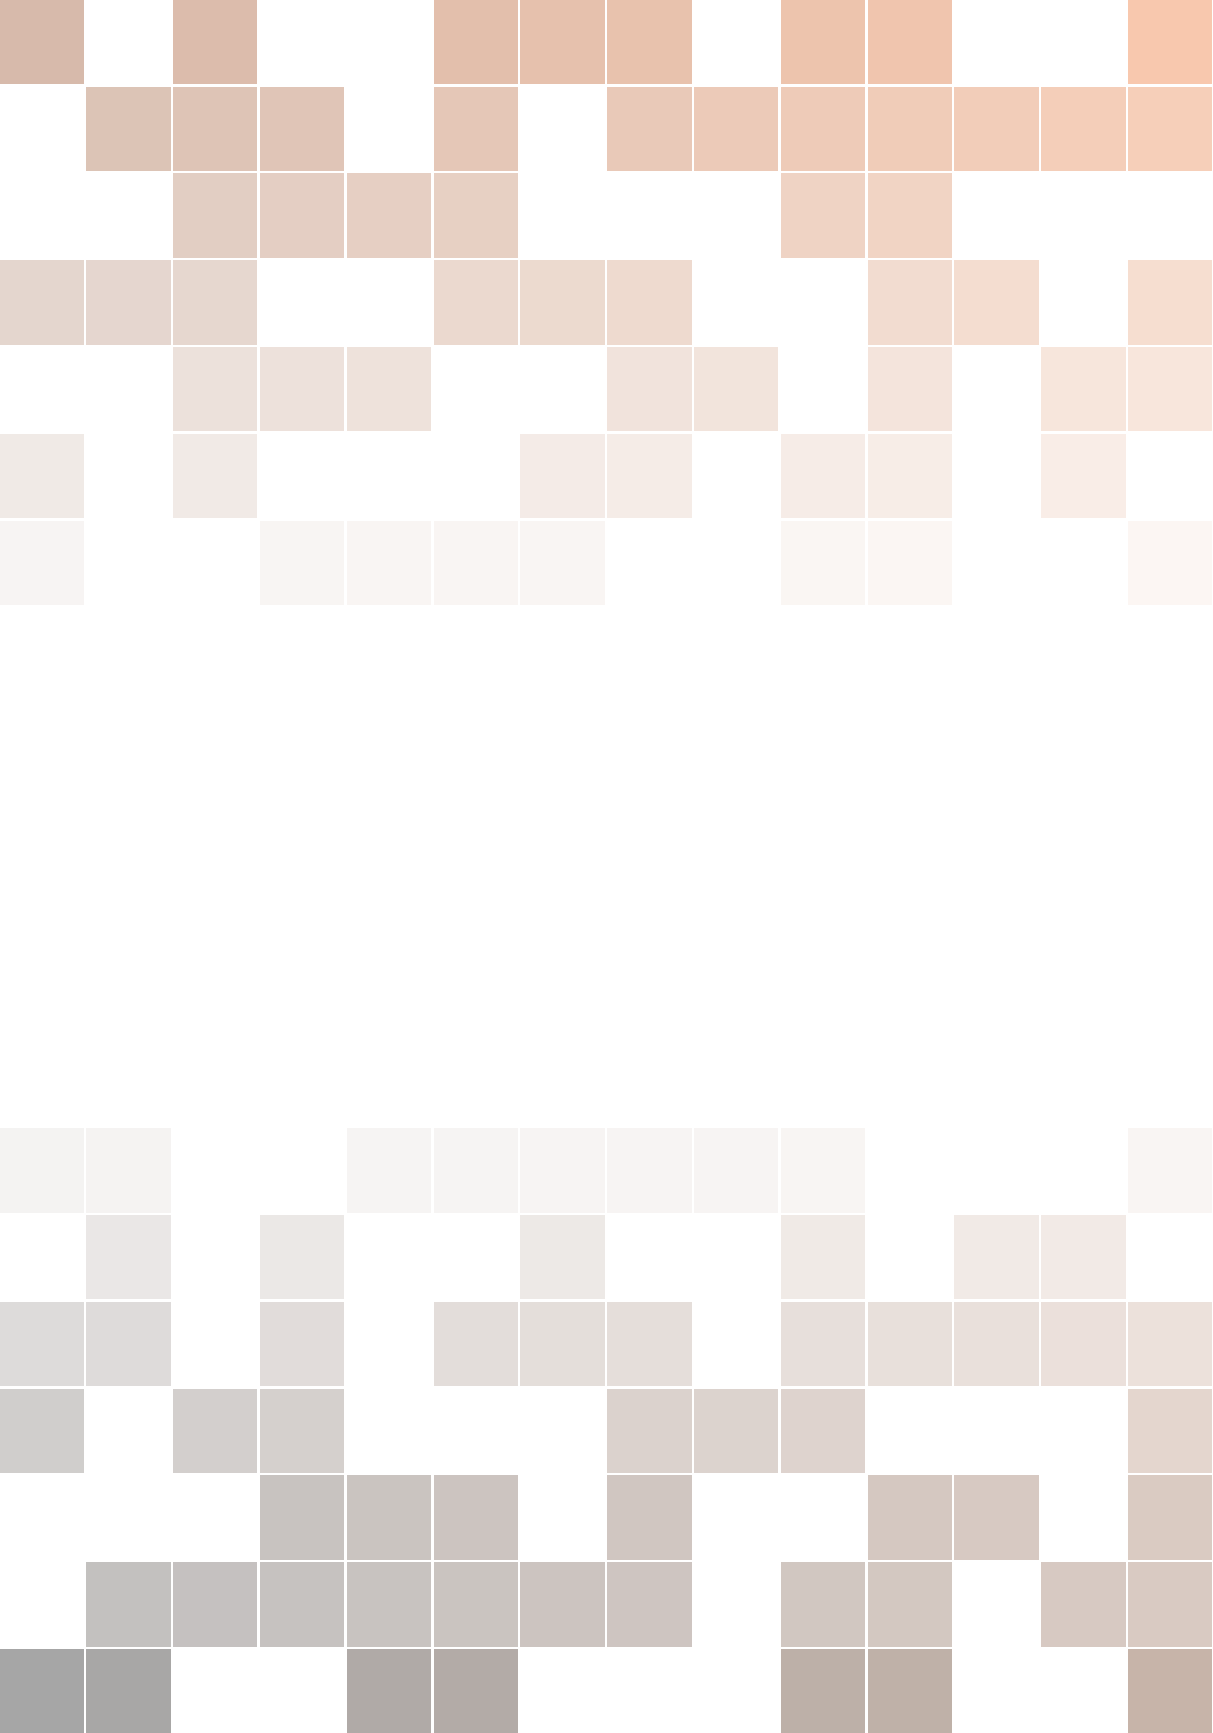
\includegraphics[width=\paperwidth]{background}};
\draw (current page.center) node [fill=ocre!30!white,fill opacity=0.6,text opacity=1,inner sep=1cm]{\Huge\centering\bfseries\sffamily\parbox[c][][t]{\paperwidth}{\centering Note ed esercizi di fluidodinamica\\[15pt] % Book title
%{\Large}\\[20pt] % Subtitle
%{\huge D. Montagnani}
}}; % Author name
\end{tikzpicture}
\vfill
\endgroup

%-------------------------------------------------------------------------------
%	COPYRIGHT PAGE
%-------------------------------------------------------------------------------

\newpage
~\vfill
\thispagestyle{empty}

\noindent Copyright \copyright\ 2019 Davide Montagnani\\ % Copyright notice

% \noindent \textsc{Published by Publisher}\\ % Publisher

% \noindent \textsc{book-website.com}\\ % URL

\noindent Licensed under the Creative Commons Attribution-NonCommercial 3.0 Unported License (the ``License''). You may not use this file except in compliance with the License. You may obtain a copy of the License at \url{http://creativecommons.org/licenses/by-nc/3.0}. Unless required by applicable law or agreed to in writing, software distributed under the License is distributed on an \textsc{``as is'' basis, without warranties or conditions of any kind}, either express or implied. See the License for the specific language governing permissions and limitations under the License.\\ % License information

\noindent \textit{First edition, March 2013} % Printing/edition date

% %--------------------------------------------------------------------------------
% %	TABLE OF CONTENTS
% %--------------------------------------------------------------------------------
% 
%\usechapterimagefalse % If you don't want to include a chapter image, use this to toggle images off - it can be enabled later with \usechapterimagetrue

\chapterimage{blank_fig} % chapter_head_1.pdf} % Table of contents heading image

\pagestyle{empty} % No headers

% \tableofcontents % Print the table of contents itself
% 
% \cleardoublepage % Forces the first chapter to start on an odd page so it's on the right

\pagestyle{fancy} % Print headers again

\dominitoc[n]
\tableofcontents


%--------------------------------------------------------------------------------
%	PART 1
%--------------------------------------------------------------------------------

\part{Esercizi}

% 01. statica --------------------------
\chapterimage{blank_fig}
\chapter{Statica}\index{Statica}\label{ch:statica}

%
\section{Definizione di fluido}
Un fluido è un materiale che non è in grado di sopportare sforzi di taglio, quando è in quiete o in moto con velocità uniforme in un sistema di riferimento inerziale (invarianza galileiana).
I fluidi ``ordinari'' sono isotropi, cioè sono indipendenti dall'orientazione nello spazio.
Un fluido isotropo in quiete è quindi caratterizzato da uno stato di sforzo idrostatico,
\begin{equation}
 \mathbb{T}^{(s)} = - p \mathbb{I} \ ,
\end{equation}
avendo indicato con $\mathbb{T}^{(s)}$ il tensore degli sforzi in quiete, $p$ la pressione all'interno del fluido e $\mathbb{I}$ il tensore identità. Il vettore sforzo $\bm{t_n}$ \textit{agente su} una superficie di fluido con normale $\bm{\hat{n}}$ si ottiene tramite il \textbf{teorema di Cauchy} per i mezzi continui
\begin{equation}
 \bm{t_n} = \bm{\hat{n}} \cdot \mathbb{T} \ ,
\end{equation}
 che lega il vettore sforzo al tensore degli sforzi tramite il versore normale alla superficie considerata, e che nel caso di fluido in quiete, diventa
\begin{equation}
 \bm{t_n}^{(s)} = \bm{\hat{n}} \cdot \mathbb{T}^{(s)}  = - p \bm{\hat{n}} \ .
\end{equation} 
Per il principio di azione e reazione, lo sforzo agente su un materiale a contatto con un fluido è di intensità uguale e direzione opposta. La risultante $\bm{R}$ delle forze agenti su un volume di fluido $V$ è data dalla somma dell'integrale su $V$ delle forze di volume $\bm{f}$ e dell'integrale sulla superficie $S$, contorno del volume $V$, del vettore sforzo $\bm{t_n}$,
\begin{equation}
 \bm{R} = \int_V \bm{f} + \oint_S \bm{t_n} \ . 
\end{equation}

%
\section{Equazione di equilibrio: forma integrale e differenziale}
Un sistema meccanico è in equilibrio quando la risultante delle forze esterne e la risultante dei momenti esterni agenti sul fluido sono nulle,
\begin{equation}
\begin{cases}
 \bm{0} = \bm{R}^{ext} \\
 \bm{0} = \bm{M}^{ext}  \ .
\end{cases} 
\end{equation}
 Per un mezzo continuo non polare, è possibile dimostrare che l'equilibrio ai momenti si riduce alla condizione di simmetria del tensore degli sforzi.
L'equilibrio delle forze agenti su un volume di fluido $V$ in quiete, delimitato dalla superficie $\partial V = S$, soggetto a forze per unità di volume $\bm{f}$ in $V$ e forze per unità di superficie $\bm{t_n}=-p \bm{\hat{n}}$ su $S$ diventa
\begin{equation}
 \bm{0} = \bm{R}^{ext} = \int_V \bm{f} + \oint_S \bm{t_n} = \int_V \bm{f} - \oint_S p \bm{\hat{n}} \ .
\end{equation}
La condizione appena ottenuta è una \textbf{condizione di equilibrio integrale}, per l'intero volume fluido $V$. Se il campo di pressione $p$ è sufficientemente regolare, è possibile applicare il teorema del gradiente (\ref{thm:grad}) all'integrale di superficie e raccogliere i termini a destra dell'uguale sotto un unico integrale di volume $V$,
\begin{equation}
 \bm{0} = \int_V \left( \bm{f} - \bm{\nabla} p \right) \ .
\end{equation}
Poiché la condizione di equilibrio deve essere valida indipendentemente dal volume $V$ considerato, imponendo che l'integranda sia identicamente nulla, si ottiene l'\textbf{equazione di equilibrio in forma differenziale}
\begin{equation}\label{eqn:statica:diff}
 \bm{f}(\bm{r}) - \bm{\nabla} p (\bm{r}) = \bm{0} \ ,
\end{equation}
dove è stata esplicitata la dipendenza dei campi $\bm{f}$, $p$ dall coordinata spaziale $\bm{r}$. Nel caso in cui sia noto il campo di forze di volume $\bm{f}$ all'interno del dominio considerato, l'equazione differenziale alle derivate parziali (\ref{eqn:statica:diff}), con le opportune condizioni al contorno, permette di calcolare il campo di pressione $p(\bm{r})$. 

\section{Legge di Stevino}
La legge di Stevino descrive il campo di pressione come funzione della quota, nelle vicinanze della superficie terrestre. La legge di Stevino viene ricavata dall'integrazione dell'equilibrio in forma differenziale (\ref{eqn:statica:diff}), nel caso in cui le forze di volume siano dovute alla gravità $\bm{f}(\bm{r}) = \rho(\bm{r}) \bm{g}(\bm{r})$, avendo indicato con $\rho(\bm{r})$ la densità del fluido e con $\bm{g}$ il campo di accelerazione gravitazionale,
\begin{equation}\label{eqn:statica:diff:g}
    - \bm{\nabla} p(\bm{r}) + \rho(\bm{r}) \bm{g}(\bm{r}) = \bm{0} \ .
\end{equation}
Nell'ipotesi di essere sufficientemente vicino alla terra da poter considerare il campo vettoriale $\bm{g}$ uniforme e diretto verso il basso lungo la normale alla superficie terrestre, è possibile scrivere l'equazione precedente in un sistema di coordinate cartesiane. Orientando l'asse $z$ verso l'alto lungo la normale alla superficie, le tre componenti cartesiane dell'equazione vettoriale sono
\begin{equation}
\begin{cases}
 \partial p(x,y,z) / \partial x = 0 \\
 \partial p(x,y,z) / \partial y = 0 \\ 
 \partial p(x,y,z) / \partial z = - \rho(x,y,z) g \ .
\end{cases}
\end{equation}
Dalle prime due equazioni si ricava che il campo di pressione non può dipendere dalle coordinate $x$, $y$ ed è quindi solo funzione di $z$. Poiché il campo di pressione dipende solo da $z$, $p = P(z)$, la terza equazione diventa un'equazione differenziale ordinaria,
\begin{equation}\label{eqn:statica:Pz}
  \dfrac{d P}{d z} = -\rho(x,y,z) g \ ,
\end{equation}
alla quale deve essere aggiunta una condizione al contorno del tipo $P(z_0) = p_0$.\footnote{In generale, servono delle condizioni di compabibilità dei dati affinché il problema sia risolvibile. Ad esempio, non dovrebbe essere difficile convincersi che il campo di densità deve dipendere solo dalla coordinata $z$ nel caso considerato.}
Senza ulteriori ipotesi, il problema composto dall'equazione (\ref{eqn:statica:Pz}) e dalla condizione al contorno necessaria ha come incognite il campo di pressione $P$ e il campo di densità $\rho$. 
In generale, per risolvere il problema è necessario la legge di stato del fluido che mette in relazione i due campi.
%
\newline \noindent
Nell'ipotesi che la densità $\rho$ e la forza di gravità siano costanti, la soluzione del problema (\ref{eqn:statica:Pz}) coincide con la \textit{legge di Stevino},
\begin{equation}
 p(z) + \rho g z = p_0 = \text{cost} \ ,
\end{equation}
avendo orientato l'asse $z$ verso l'alto e imposto la condizione al contorno in $z_0 = 0$.
% Nel caso in cui la densità non sia costante, ma che dipenda dallo stato termodinamico, per risolvere il problema è necessaria l'equazione di stato del fluido.
\begin{exercise}\label{exe:stdatm:cart}
    Utilizzando la legge di stato dei gas perfetti per l'aria, $P = \rho R T$, e l'approssimazione lineare dell'andamento della temperatura con la quota $z$, con gradiente termico $dT/dz=a=-6.5\degree/km$, si ricavi l'andamento con la quota $z$ delle variabili termodinamiche $(P,\rho, T)$ per l'atrmosfera standard. Si trascuri l'andamento di $g$ con la quota. Trascurando la curvatura terrestre, si utilizzi un sistema di coordinate cartesiane per scrivere le componenti dell'equazione vettoriale (\ref{eqn:statica:diff:g}).
\end{exercise}
\begin{exercise}\label{exe:stdatm:sphe}
    Utilizzando la legge di stato dei gas perfetti per l'aria, $P = \rho R T$, e l'approssimazione lineare dell'andamento della temperatura con la quota $r$, con gradiente termico $dT/dr=a=-6.5\degree/km$, si ricavi l'andamento con la quota $r$ delle variabili termodinamiche $(P,\rho, T)$ per l'atrmosfera standard, senza trascurare l'effetto della curvatura terrestre. Si utilizzi un sistema di coordinate sferiche per scrivere le componenti dell'equazione vettoriale (\ref{eqn:statica:diff:g}). Si valuti poi l'errore che si commette nell'esercizio \ref{exe:stdatm:cart} trascurando la curvatura terrestre sul calcolo delle variabili termodinamiche a quota $z = 10 \ km$.
\end{exercise}
%
\section{Galleggiamento di un corpo immerso in un fluido}
Un corpo immerso in fluido riceve dal basso verso l'alto una spinta uguale al peso della massa del fluido spostato. Se un corpo di volume $V_s$ immerso in un fluido $\rho_f$ ne sposta un volume $\tilde{V}_f$, su di esso agisce una forza (di Archimede o di galleggiamento)
\begin{equation}
    \bm{F}_{Arch} = - \rho_f \tilde{V}_f \bm{g} = - \int_{\tilde{V}_f} \rho_f \bm{g} \ .
\end{equation}
La legge di Archimede vale per un sistema immerso nel campo di gravità $\bm{g}$, uniforme in spazio.
\newline \noindent
Forze di galleggimento nascono su un corpo immerso in un fluido in cui c'è un gradiente di pressione. La legge di Archimede è solo un caso particolare di galleggiamento, forse il più evidente, per il quale il campo di gravità è all'origine del gradiente di pressione. In generale, la forza di galleggiamento su un corpo immerso completamente in un fluido vale
\begin{equation}
    \bm{F}_{gall} = -\int_{S_s} p \bm{\hat{n}} = - \int_{V_s} \bm{\nabla} p \ .
\end{equation}
Un esempio di galleggiamento di interesse aeronautico si incontra quando si svolge un esperimento in galleria del vento, se nella camera di prova è presente un gradiente di pressione diretto nella direzione $\bm{\hat{x}}$ della corrente. Se in prima approssimazione si considera un gradiente di pressione $\bm{\nabla}p = - G_P \bm{\hat{x}}$, $G_P>0$ e costante, si può stimare la forza di galleggiamento $\bm{F}_{gall} = V_s G_P \bm{\hat{x}}$ dovuta al gradiente di pressione in galleria del vento, assente in condizioni di aria libera. Questa azione contribuisce al valore misurato della resistenza del modello.
%
La valutazione di questa azione ``spuria'' sul corpo e la correzione delle misure effettuate rientrano nell'ambito delle \textit{correzioni di galleria}.

% \vspace{3cm}


% \section{Risultante e punto di applicazione delle forze di galleggiamento: equilibrio e stabilità di corpi galleggianti}

\vspace{10pt}
Si ritorna ora sulla legge di Archimede che descrive le forza di galleggiamento che un fluido esercita su un corpo immerso. Nel problema di un corpo immerso in un fluido, la risultante delle forze di galleggiamento entra nell'equazione di equilibrio del corpo in direzione verticale (direzione della gravità, \textbf{g}). Il punto di applicazione della risultante delle forze di galleggiamento e la sua posizione relativa rispetto al baricentro del corpo influenzano la stabilità delle condizioni di equilibrio.

\subsection{Risultante delle forze: legge di Archimede}
%
\begin{figure}[t]
 \centering
 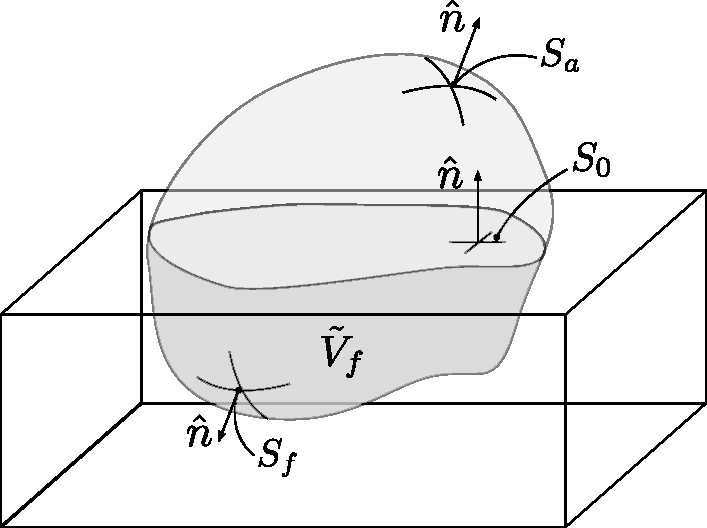
\includegraphics[width=0.5\textwidth]{./fig/archimede_01}
 \caption{Suddivisione delle superfici e dei volumi per la dimostrazione della legge di Archimede.}\label{fig:archimede_01}
\end{figure}
%
Si considera il problema di un corpo immerso in un fluido di densità uniforme $\rho$ molto maggiore della densità dell'aria: la pressione agente sulla superficie del corpo esposta all'aria si può considerare costante, uguale a $p_a$.
La legge di Stevino descrive la distribuzione di pressione all'interno del fluido. Si sceglie l'asse $z$ in direzione verticale, così che il campo di gravità è $\bm{g} = -g \bm{\hat{z}}$. Scegliendo l'origine dell'asse $z$ in corrispondenza del pelo libero, la pressione all'interno del fluido vale $p(z) = p_a - \rho g z$, per $z < 0$. Facendo riferimento alla figura \ref{fig:archimede_01}, si può calcolare la risultante delle forze $\bm{R}$ come
\begin{equation}
\begin{aligned}
    \bm{R} & = - \oint_{S} p \bm{\hat{n}} = 
               - \int_{S_a} p \bm{\hat{n}} - \int_{S_f} p \bm{\hat{n}} = \\
        & =    - \int_{S_a} p_a \bm{\hat{n}} - \int_{S_f} p_a \bm{\hat{n}} + 
                 \int_{S_f} \rho g z \bm{\hat{n}} = \\
        & =    - \underbrace{\int_{S} p_a \bm{\hat{n}}}_{=0} + 
                 \int_{S_f} \rho g z \bm{\hat{n}} = \\
        & =      \int_{S_f} \rho g z \bm{\hat{n}} + 
                 \underbrace{\int_{S_0} \rho g z \bm{\hat{n}}}_{=0, \ z|_{S_0} = 0} =
                 \oint_{\tilde{S}_f} \rho g z \bm{\hat{n}} = 
                 \int_{\tilde{V}_f} \rho g \bm{\hat{z} } = 
                 \rho \tilde{V}_f g \bm{\hat{z}} = 
                 M_{\tilde{V}_f} g \bm{\hat{z}} \ ,
\end{aligned}
\end{equation}
avendo sommato l'integrale nullo $\int_{S_0} \rho g z \bm{\hat{n}}$, per poter ottenere l'integrale di $\rho g z$ sulla superficie $\tilde{S}_f = S_f \cup S_0$ e applicare il teorema del gradiente (\ref{thm:grad}).
Come stabilito dal principio di Archimede, la risultante delle forze di galleggiamento $\bm{R}$ agenti sul corpo agisce dal basso verso l'alto con un'intensità pari al peso del volume di fluido spostato, $M_{\tilde{V}_f} g$.

\subsection{Punto di applicazione}
Il punto di applicazione della forza di galleggiamento è il punto dove bisogna applicare la risultante delle forze per ottenere un sistema di azioni equivalente al sistema di azioni continuo generato dalla pressione.
Dall'equivalenza ai momenti dei due sistemi di azioni, si ottiene
\begin{equation}
\begin{aligned}
\bm{r}_O \times \bm{R} & = - \oint_{S} p \bm{r} \times \bm{\hat{n}} = 
    - \int_{S_a} p \bm{r} \times \bm{\hat{n}}
    - \int_{S_f} p \bm{r} \times \bm{\hat{n}} = \\
& = - \int_{S_a} p_a \bm{r} \times \bm{\hat{n}}
    - \int_{S_f} p_a \bm{r} \times \bm{\hat{n}} 
    + \int_{S_f} \rho g z \bm{r} \times \bm{\hat{n}} = \\
& = - \underbrace{\int_{S} p_a \bm{r} \times \bm{\hat{n}}}_{=0} + 
      \int_{S_f} \rho g z \bm{r} \times \bm{\hat{n}} = \\
& =   \int_{S_f} \rho g z \bm{r} \times \bm{\hat{n}} + 
      \underbrace{\int_{S_0} \rho g z \bm{r} \times \bm{\hat{n}}}_{=0, \ z|_{S_0} = 0} =\\
& =  \oint_{\tilde{S}_f} \rho g z \bm{r} \times \bm{\hat{n}} = 
     \oint_{\tilde{S}_f} \rho g \delta_{\ell z} r_{\ell} \epsilon_{ijk} r_j n_k = 
     \rho g \int_{\tilde{V}_f} \dfrac{\partial}{\partial r_k}( \delta_{\ell z} r_{\ell} \epsilon_{ijk} r_j ) = \\
    & = \rho g \int_{\tilde{V}_f} \delta_{\ell z} \epsilon_{ijk}\left(  \dfrac{\partial r_{\ell}}{\partial r_k} r_j + r_{\ell} \dfrac{\partial r_j}{\partial r_k} \right) = \\ 
    & = \rho g \int_{\tilde{V}_f} \delta_{\ell z} \epsilon_{ijk}\left( \delta_{\ell k}r_j + r_{\ell} \delta_{jk} \right) = \\
    & = \rho g \int_{\tilde{V}_f} \epsilon_{ijz} r_j + \delta_{\ell z} \underbrace{\epsilon_{ijj}}_{ = 0} r_{\ell} = \\
    & = \rho g \int_{\tilde{V}_f}  \bm{r} \times \bm{\hat{z}} \ .
\end{aligned}
\end{equation}
Usando un sistema di assi catesiani e ricordando che $\bm{R} = R \bm{\hat{z}}$, si può scomprre l'equazione nelle componenti non nulle, $x$ e $y$, 
\begin{equation}
\begin{cases}
   x_0 R = \rho g \displaystyle\int_{\tilde{V}_f} x \\ \\
   y_0 R = \rho g \displaystyle\int_{\tilde{V}_f} y 
\end{cases} \qquad \rightarrow \qquad
\begin{cases}
    x_0 = \dfrac{\rho g}{R}  \displaystyle\int_{\tilde{V}_f} x  
        = \dfrac{1}{\tilde{V}_f}  \displaystyle\int_{\tilde{V}_f} x 
    \\ \\
    y_0 = \dfrac{\rho g}{R}  \displaystyle\int_{\tilde{V}_f} y 
        = \dfrac{1}{\tilde{V}_f}  \displaystyle\int_{\tilde{V}_f} y \ .
\end{cases}
\end{equation}


\subsection{Stabilità statica dell'equilibrio}


% \section{}





\newpage

\section{Esercizi}
\noindent
\begin{tabular}{cc}
\begin{minipage}{0.60\textwidth}
%\sectionIf{\flagSect}{\taitol{Esercizio}}
\begin{exercise}[Legge di Archimede]
Si consideri, sulla superficie terrestre, un recipiente di diametro $D=2 \ m$ e profondit\`a $H=
3\  m$
contenente acqua ($\rho = 998\ kg / m^3$). Al suo interno \`e inserita una sfera di raggio $a=0.2\, m$
e densit\`a pari a $\rho_s=842.06\ kg / m^3$.
Determinare in modo univoco la posizione assunta dalla sfera nel
liquido. Tale posizione varia se invece che sulla terra ci si trova
sulla luna?\\ 
($h=0.3\  m$, non varia sulla luna.)
\end{exercise}
\end{minipage}
&
\begin{minipage}{0.35\textwidth}
   \begin{center}
   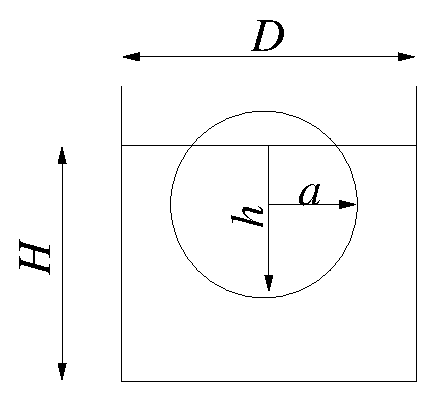
\includegraphics[width=0.90\textwidth]{./fig/recipientesfera.eps}
   \end{center}
\end{minipage}
\end{tabular}

%\vspace{1.0cm}
%\textbf{Soluzione.}

\sol

\partone
Legge di Archimede. Condizione di equilibrio. Calcolo del volume di solidi  (integrali di volume). Adimensionalizzazione. Soluzione di semplici equazioni non lineari per via grafica (studio di funzione) e/o numerica.

\parttwo
Per svolgere l'esercizio bisogna calcolare la condizione di equilibrio del corpo, soggetto alla propria forza peso e alla forza che il fluido esercita su di esso (legge di Archimede). Nell'equazione di equilibrio, l'incognita $h$ compare nella formula del volume immerso nel fluido. L'equazione di equilibrio è un'equazione non lineare in $h$, da risolvere per via grafica
o numerica.
\begin{itemize}
  \item Scrittura dell'equazione di equilibrio del corpo soggetto al proprio peso e alla forza esercitata su di esso dal fluido, diretta verso
  l'alto e pari al peso del volume del fluido spostato (legge di Archimede).
    \begin{equation}\label{eqn:equil_archimede}
      \rho_s V_s g = \rho V_c g \quad\Rightarrow\quad \rho_s V_s = \rho V_c
    \end{equation}
    
  \textit{Osservazione.} Si trova subito la risposta all'ultimo quesito: poiché $g$ non compare nell'equazione di equilibrio, la condizione di equilibrio sulla Luna è uguale a quella che si ha sulla Terra.
  \item Calcolo del volume della sfera e della calotta sferica:

   \begin{itemize}    
     \item Volume della sfera: $V_s = \frac{4}{3}\pi a^3$ %(vergogna se non lo si sa subito!!!)
    
     \item Volume della calotta sferica: $V_c = \pi h^2 (a - \frac{h}{3})$
     
      (per credere, verificare casi limite: $h=0$, $h=a$, $h=2a$; alla fine dell'esercizio è riportato il calcolo, tramite un integrale di volume)
    \end{itemize}
    
  \item Le formule per i volumi $V_c$ e $V_s$ sono inserite nell'eq.
   \ref{eqn:equil_archimede}. L'equazione viene semplificata e scritta in forma adimensionale, introducendo la variabile $x=\frac{h}{a}$, per mettere in evidenza il parametro che governa il problema, cioè il rapporto di densità $\rho_s/\rho$. L'equazione di terzo grado in x viene risolta, considerando i limiti fisici del problema ($0 \le x \le 2$):
    \begin{equation}
      \rho \pi h^2 \Big(a-\frac{h}{3}\Big) = \rho_s \frac{4}{3}\pi a^3  \quad\Rightarrow\quad
      \frac{3}{4} x^2 \Big(1 - \frac{x}{3}\Big) = \frac{\rho_s}{\rho}
    \end{equation}
  Alcuni metodi per risolvere equazioni non lineari possono essere ad esempio:
  \begin{itemize}
    \item metodi iterativi. Ad esempio metodo di Newton
    \begin{center}
\begin{verbatim}
x          res 
1.0000    -3.437475e-01  
1.4583    -2.406993e-02  
1.4990    -5.841602e-04  
1.5000    -4.027539e-07  
1.5000    -1.924017e-13
\end{verbatim}
\end{center}
    
    \item metodo grafico (educativo: per problemi più complicati, prima di calcolare le soluzioni con metodi
    numerici, è bene avere un'idea di cosa si sta cercando).
    Si cercano le intersezioni delle funzioni $f_1(x) = \frac{3}{4} x^2 \Big(1 - \frac{x}{3}\Big)$ e $f_2(x) = \frac{\rho_s}{\rho}$.
  
\begin{center}
\begin{tikzpicture}
\begin{axis}[axis lines=middle, domain=-1.2:3.2, xlabel={$x=\frac{h}{a}$}, ylabel={$y=\frac{\rho_s}{\rho}$}]
\addplot
[domain=0:2,samples=40,smooth,thick,blue]
{3/4 * (x^2 * (1-x/3))};
\addplot
[domain=-1.2:3.2,samples=40,smooth,thick,red]
{842.06/998};
\addplot
[domain=-1.2:3.2,samples=40,smooth,dashed,blue]
{3/4 * (x^2 * (1-x/3))};
\addplot
[domain= 2.0:3.2,samples=40,smooth,thick,blue]
{1.0};
\addplot
[domain=-1.2:0.0,samples=40,smooth,thick,blue]
{0.0};
\addplot[color=black,mark=x] coordinates{
         (1.50, 0)
         (1.50, 0.842)};
\legend{$f_1(x)$,$\frac{\rho_s}{\rho}=0.842$}
\end{axis}
\end{tikzpicture}
\end{center}
    
  \end{itemize}
  
\end{itemize}

\textit{Osservazione.} Per valori di $\frac{\rho_s}{\rho}$ compresi tra
 0 e 1, esiste una e una sola soluzione fisica del problema.
% Come giustamente \textbf{suggerito da un vostro compagno},
 Per i valori di desità
 ``estremi'' $\rho_s = 0$ (la sfera non pesa niente), $\rho_s = \rho_f$ (la sfera
 ha la stessa densità del fluido), esistono infinite soluzioni:
 ad esempio, nel caso di $\rho_s = \rho_f$ la posizione di equilibrio è indipendente
 dalla profondità alla quale è posta la sfera. Nel grafico, la funzione
 $f_1(x)$ rappresenta il volume immerso della sfera (diviso il volume totale
 della sfera stessa) al variare della 
 distanza $h$ del punto più basso dal pelo libero: questa deve quindi
 essere rappresentata, come in figura, nulla per valori di $x<0$ (sfera
 completamente fuori dall'acqua), con il ramo di cubica per $0<x<2$
 (sfera parzialmente immersa), uguale a $1$ per $x>2$ (sfera completamente
 immersa). La funzione $f_1(x)$ può quindi essere definita a tratti:
 \begin{equation}
  f_1(x) = 
 \begin{cases}
   0 &    x < 0 \\
   \frac{3}{4} x^2 \Big(1 - \frac{x}{3}\Big) &    0 \leq x \leq 2 \\
   1 &   x > 2 \\
 \end{cases}
 \end{equation}
\vspace{0.2cm}

\textit{Discussione dei risultati.} Quando diminuisce la denistà relativa
 del solido, la linea rossa si abbassa e la soluzione $x=\frac{h}{a}$
 diminuisce (la sfera ha una porzione maggiore al di fuori dall'acqua).
 Esiste una e una sola soluzione che abbia senso fisico, fino a quando
 la densità relativa è compresa tra 0 e 1: non ha senso considerare valori
 negativi (la densità è una quantità positiva), mentre per valori di
 $\frac{\rho_s}{\rho}$ maggiori di 1 non può esistere una condizione
 di equilibrio statico (la sfera affonda...).


\newpage
\textbf{Calcolo volume cupola sferica.} 
\'E comodo svolgere il calcolo in coordinate cilindriche $(r,\theta,z)$.
Il volume $V_{im}$ della parte immersa è uguale a 
\begin{equation}
\begin{aligned}
V_{im} = \iiint_{V_{im}} dV & = \int_{\theta=0}^{2\pi} \int_{z=-a}^{l} \int_{r=0}^{\sqrt{a^2-z^2}} dV \\
                & = \int_{\theta=0}^{2\pi} \int_{z=-a}^{l} \int_{r=0}^{\sqrt{a^2-z^2}} r dr dz d\theta \\
                & = 2\pi \int_{z=-a}^{l} \frac{a^2-z^2}{2} dz \\
                & = \frac{\pi}{3} [2 a^3 + 3 a^2 l - l^3]
\end{aligned}
\end{equation}

Definendo $h = R+l$ come la quota immersa della sfera, si ottiene:
\begin{equation}
V_{im} = \pi h^2 \displaystyle \left( a - \frac{h}{3} \right)
\end{equation}



\newpage

\noindent
\begin{tabular}{cc}
\begin{minipage}{0.60\textwidth}
%\sectionIf{\flagSect}{\taitol{Esercizio}}
\begin{exercise}[Stevino: serbatoi]
Si consideri il sistema rappresentato in figura in cui un recipiente
aperto all'atmosfera, contenente olio con densit\`a $\rho= 800\ kg/m^3$, \`e
collegato tramite una tubazione a un secondo recipiente, contenente a
sua volta olio e aria non miscelati. Date le due altezze $h_1=1.5\ m$ e $h_2= 1.8 \ m$
del pelo libero nei due recipienti e l'altezza $H= 2.5\ m$ della tubatura,
determinare il valore della pressione nei punti A e B in figura,
esprimendolo sia in Pascal sia in metri d'acqua. Considerare la
pressione atmosferica standard ($101325\ Pa$).\\ 
($p_A=93477\ Pa = 9.53\ m_{H_2O}$, $p_B=98970.6\ Pa=10.10\ m_{H_2O}$.)
\end{exercise}
\end{minipage}
&
\begin{minipage}{0.35\textwidth}
   \begin{center}
   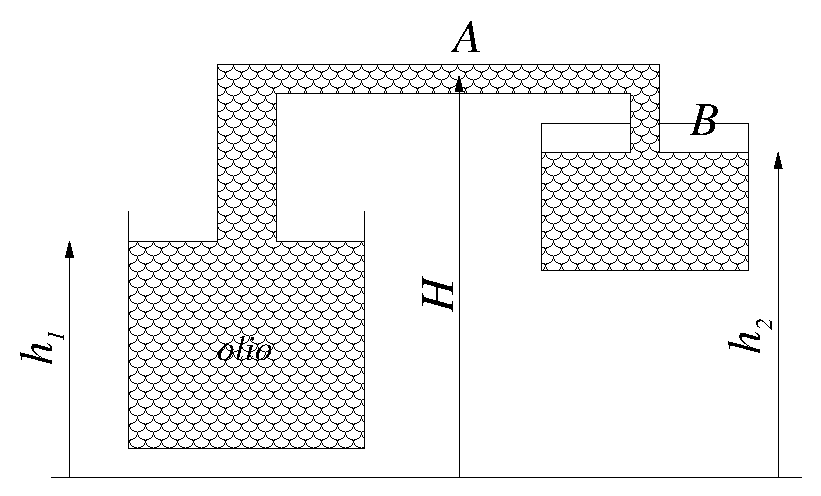
\includegraphics[width=0.90\textwidth]{./fig/recipientiariaolio.eps}
   \end{center}
\end{minipage}
\end{tabular}

\sol

\partone
Legge di Stevino, $P_1 + \rho g h_1 = P_2 + \rho g h_2 $.
%
Conversione $Pa$ - metri di $H_2O$, 
\begin{equation}
1 m_{{H_2O}} = P[Pa] = \rho_{H_2O} \cdot g \cdot 1 m =
9810 \dfrac{kg}{m^2 s^2} \cdot 1 m = 9810 Pa \ . 
\end{equation}

\parttwo
 Il problema si risolve applicando due volte la legge di Stevino e la conversione da Pascal $Pa$ a metri d'acqua $m_{H_2O}$.
Sia $O$ il punto sul pelo libero nel serbatoio \textit{aperto} di sinistra, sul quale agisce la pressione ambiente.

\begin{equation}
\begin{cases}
  P_A = P_O + \rho g (h_1 - H)  = 93477 Pa = \dfrac{93477}{9810} m_{H_2O} = 9.53 m_{H_2O}  & \text{(Stevino O-A)} \\ \\
  P_B = P_O + \rho g (h_1 - h_2) = 98970.6 Pa = \dfrac{98970.6}{9810} m_{H_2O}= 10.10 m_{H_2O} & \text{(Stevino O-B)}
\end{cases}
\end{equation}


\newpage

\noindent
\begin{tabular}{cc}
\begin{minipage}{0.60\textwidth}
%\sectionIf{\flagSect}{\taitol{Esercizio}}
\begin{exercise}[Azioni statiche: diga]
Si consideri la sezione di diga rappresentata in figura.
Si determini il modulo e la direzione del risultante 
delle forze per unit\`a di apertura agente sui diversi 
tratti rettilinei della diga stessa sapendo che la pressione
atmosferica \`e di $1.01 \times 10^5\ Pa$. Dimensioni: $a=10\ m$,
$b=2\, m$, $c=8\ m$, $d=10\ m$, $e=5\ m$, $f=3\ m$.\\ 
($\bm{R}_1=347100\hat{\bm{x}}\  N/m$,   \\
 $\quad \bm{R}_2=- 1043200\hat{\bm{z}}\ N/m$, \\
 \quad $\bm{R}_3=774500\hat{\bm{x}}\ N/m$,    \\
 \quad $\bm{R}_4=2284000 N/m \bm{\hat{x}} + 2284000 N/m \bm{\hat{z}}$,  \\
 \quad $\bm{R}_5=2774000\hat{\bm{z}}\ N/m$.)
\end{exercise}
\end{minipage}
&
\begin{minipage}{0.35\textwidth}
   \begin{center}
   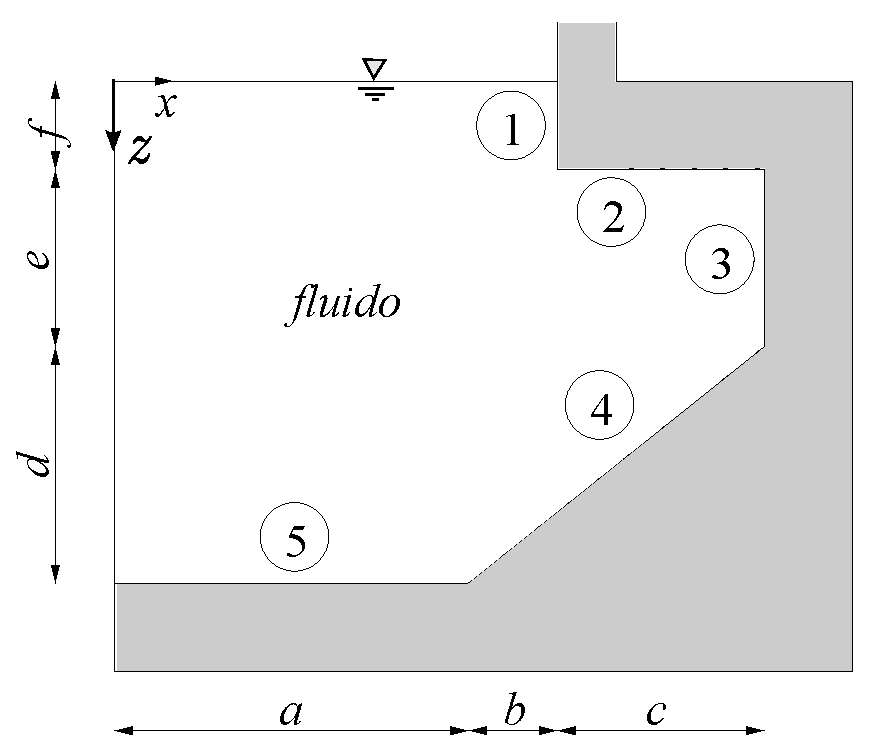
\includegraphics[width=0.90\textwidth]{./fig/diga2.eps}
   \end{center}
\end{minipage}
\end{tabular}


\sol

\partone
Legge di Stevino, $P_1 + \rho g h_1 = P_2 + \rho g h_2$.
%
 Calcolo della risultante delle azioni statiche, data la distribuzione di pressione e la normale $\bm{\hat{n}}$ uscente dal volume fluido,
\begin{equation}
   \bm{R} = \int_{S} P \bm{\hat{n}} \ .
\end{equation}

\parttwo
 Si risolve il problema bidimensionale, al quale ``manca'' la dimensione perpendicolare al piano del disegno. La risultante per unità di apertura agente sul lato $\ell$ (unità di misura nel SI, $N/m$) sarà quindi il risultato dell'integrale di linea
\begin{equation}
   \bm{R} = \int_{\ell} P \bm{\hat{n}} \ .
\end{equation} 
 Per ogni lato si calcola la distribuzione di pressione, grazie alla legge di Stevino. Si integra la distribuzione di pressione per ottenere il modulo della risultante; la direzione coincide con quella della normale (uscente dal volume occupato dal fluido).
Per lo svolgimento, è stato scelto il sistema di riferimento rappresentato in figura, con l'asse x diretto verso destra e l'asse z verso il basso.

\begin{itemize}

 \item Lato 1. Pressione lineare in z, $P(z) = P_O + \rho g z , \ z \in [0,f] $. Risultante
   \begin{equation}
   \bm{R}_1 = \int_{\ell_1} P \bm{\hat{n}} = \int_{0}^{f} (P_O + \rho g z) \bm{\hat{x}} dz = 
     \displaystyle\left(P_O  f + \frac{1}{2} \rho g f^2 \right) \bm{\hat{x}} = 347100 N/m \bm{\hat{x}}
   \end{equation}
 \item Lato 2. Pressione costante, $P = P_O + \rho g f$. Risultante 
   \begin{equation}
     \bm{R}_2 = \int_{\ell_2} P \bm{\hat{n}} = P\cdot c (-\bm{\hat{z}})=(P_O + \rho g f)\cdot c(-\bm{\hat{z}}) = - 1043200 N/m \bm{\hat{z}}
   \end{equation}
 \item Lato 3. Pressione lineare in z, $P(z) = P_O + \rho g z , \  z \in [f,f+e]$. Risultante
   \begin{equation}
     \bm{R}_3 = \int_{\ell_3} P \bm{\hat{n}} = \int_{f}^{f+e} (P_O + \rho g z) \bm{\hat{x}} dz = 
     \displaystyle\left(P_O  f + \frac{1}{2} \rho g \left[(f+e)^2 - f^2\right]\right) \bm{\hat{x}} = 774500 N/m \bm{\hat{x}}
   \end{equation}
 \item Lato 4. Pressione lineare in z, $P(z)  = P_O + \rho g z , \ z \in [f+e,f+e+d]$. Poichè il tratto di parete è rettilineo, il vettore normale è costante e può essere portato fuori dall'integrale. Si calcola prima il modulo della risultante e poi lo si moltiplica per il versore normale. Il modulo della risultante vale
   \begin{equation}
   \begin{aligned}
      {R}_4 & = \int_{\ell_4} P d\ell = \int_{f+e}^{f+e+d} P(z) \frac{\sqrt{(b+c)^2+d^2}}{d} dz = \qquad \qquad \text{$\displaystyle\left(d\ell = \frac{\sqrt{(b+c)^2+d^2}}{d} dz \right)$} \\
     & = \int_{f+e}^{f+e+d} (P_O + \rho g z) \frac{\sqrt{(b+c)^2+d^2}}{d} dz = \\
     & = \frac{\sqrt{(b+c)^2+d^2}}{d}\left[ P_O d + \frac{1}{2} \rho g \left((f+e+d)^2-(f+e)^2 \right)  \right] = 
     \sqrt{2} \cdot 2284000 N/m \\
   \end{aligned}
   \end{equation}
   La forza può essere scritta come $\bm{R}_4 = R_4 \bm{\hat{n}}_4$, con
   $\bm{\hat{n}}_4 = 1/\sqrt{2} \ \hat{\bm{x}} + 1/\sqrt{2} \ \hat{\bm{z}}$. Proietttando $\bm{R}_4$ lungo gli assi si ottengono le componenti orizzontali
   e verticali
   \begin{equation}
     \bm{R}_4 = 2284000 N/m \bm{\hat{x}} + 2284000 N/m \bm{\hat{z}}
   \end{equation}
 \item Lato 5. Pressione costante, $P = P_O + \rho g (f+e+d)$. Risultante 
   \begin{equation}
     \bm{R}_5 = P\cdot a \bm{\hat{z}} =(P_O + \rho g (f+e+d))\cdot a \bm{\hat{z}} =  2774000 N/m \bm{\hat{z}}
   \end{equation}
 
\end{itemize}


\newpage
\vspace{1.0cm}
\noindent
\begin{tabular}{cc}
\begin{minipage}{0.60\textwidth}
%\sectionIf{\flagSect}{\taitol{Esercizio}}
\begin{exercise}[Stevino: recipiente labirintico]
Si consideri il sistema di recipienti rappresentato in figura, in cui 
la zona tratteggiata contiene acqua, di densit\`a pari a $10^3\ kg/m^3$ mentre nella restante parte \`e
presente aria di densit\`a pari a $1.2\ kg/m^3$. Determinare la pressione nei punti $A$, $B$, $C$ e $D$
sapendo che le rispettive altezze sono $h_A=1\ m$, $h_B=1.4\ m$,
$h_C=1.2\ m$ e $h_D=1.6\ m$. Sia inoltre $h_0=1.3\ m$ e la pressione
esterna $P_0=101325\ Pa$.\\ 
($P_A=104262\ Pa$, $P_B=100346\ Pa$, $P_C=100348\ Pa$, $P_D=97424\ Pa$.)
\end{exercise}
\end{minipage}
&
\begin{minipage}{0.35\textwidth}
   \begin{center}
   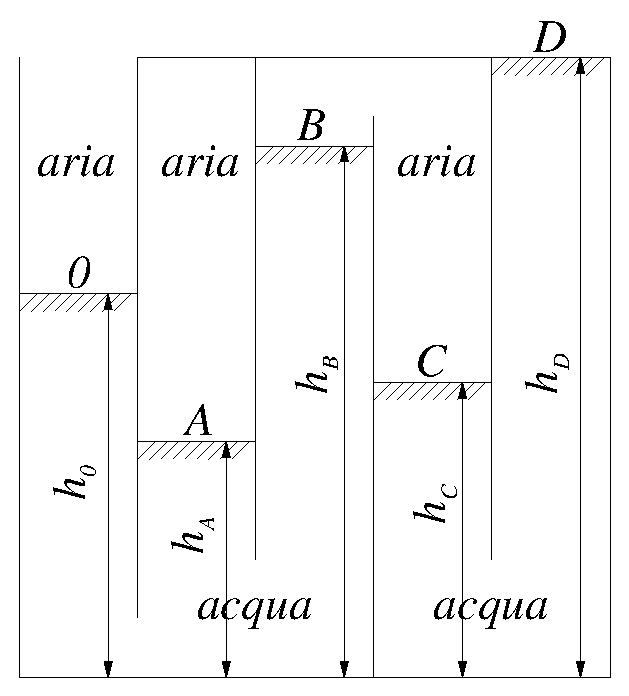
\includegraphics[width=0.90\textwidth]{./fig/tubimultipli.eps}
   \end{center}
\end{minipage}
\end{tabular}

\sol

\partone
 Legge di Stevino, $ P_1 + \rho g h_1 = P_2 + \rho g h_2$.
\vspace{0.5cm}

\parttwo
Il problema viene risolto applicando ripetutamente la legge di Stevino,
 a partire dalla superficie $0$ sulla quale agisce la pressione ambiente
 $P_0$. Nella legge di Stevino è necessario prestare attenzione ad usare
 la densità del fluido che mette in collegamento i due punti considerati.
I punti $A$ e $B$ sono messi in collegamento con il punto $0$ dall'acqua.
 I punti $B$ e $C$ sono messi in collegamento tra di loro dall'aria. I punti
 $C$ e $D$ di nuovo dall'acqua. La soluzione del problema è quindi
 
\begin{equation}
\begin{aligned}
 & P_0 = 101325 Pa & \text{dato} \\
 & P_A = P_0 + \rho g (h_0 - h_A) = ... \\
 & P_B = P_0 + \rho g (h_0 - h_B) = ... \\
 & P_C = P_B + \rho_a g (h_B - h_C) = ... \\
 & P_D = P_C + \rho g (h_C - h_D) = ... 
\end{aligned}
\end{equation}

\newpage

\noindent
\begin{tabular}{cc}
\begin{minipage}{0.60\textwidth}
%\sectionIf{\flagSect}{\taitol{Esercizio}}
\begin{exercise}[Leva idraulica]
La leva idraulica, rappresentata in figura, \`e formata da due
sistemi cilindro-pistone. 
Determinare la forza che \`e necessario applicare al secondo pistone 
per mantenere il sistema in equilibrio
quando sul primo agisce una forza $F_1 = 5000\ N$, 
allorch\'e i pistoni si trovano nella posizione indicata in figura.

Dati: diametro primo cilindro: $d_1 = 0.2\ m$; diametro secondo cilindro: 
$d_2 = 0.4\ m$; diametro del condotto che unisce i due cilindri:
$0.025\ m$;
densit\`a del fluido di lavoro: $600\ kg/m^3$;
altezza del primo pistone $h_1 = 1\ m$, altezza del secondo pistone
$h_2=2\ m$.\\ 
($p_1=159155\ Pa$, $p_2=153269\ Pa$, $\bm{F}_2=-19260.3 \hat{\bm{z}}\ N$.)
\end{exercise}
\end{minipage}
&
\begin{minipage}{0.35\textwidth}
   \begin{center}
   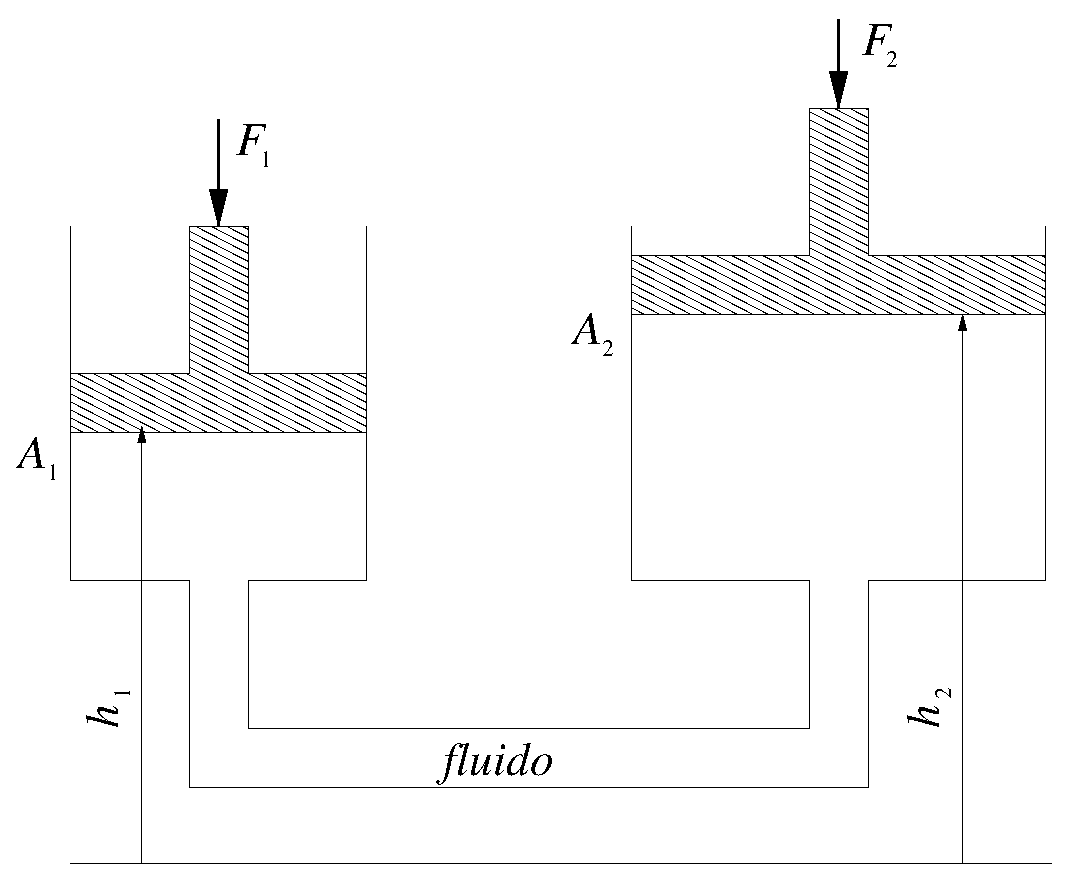
\includegraphics[width=0.90\textwidth]{./fig/leva_idraulica1.eps}
   \end{center}
\end{minipage}
\end{tabular}

\sol

\partone
 Legge di Stevino. Risultante statica. Leva idraulica.

\parttwo
 Il problema si risolve scrivendo le condizioni di equilibrio tra le forze esterne e la risultante dello sforzo di pressione sulle facce opposte dei pistoni e applicando la legge di Stevino tra le due sezioni $A_1$ e $A_2$.
Si ottiene un sistema lineare di tre equazioni in tre incognite $p_1, p_2, F_2$),
\begin{equation}
\begin{cases}
  F_1 = p_1 \pi \dfrac{d_1 ^2}{4} & \text{(Equilibrio pistone 1)} \\
  p_2 = p_1 - \rho g (h_2 - h_1) & \text{(Legge di Stevino)} \\
  F_2 = p_2 \pi \dfrac{d_2 ^2}{4} & \text{(Equilibrio pistone 2)} \ ,
\end{cases}
\end{equation}
la cui soluzione è
\begin{equation}
\Rightarrow \quad
\begin{cases}
  p_1 = \dfrac{4}{\pi} \dfrac{F_1}{d_1^2}  & = 159155 Pa \\
  p_2 = \dfrac{4}{\pi} \dfrac{F_1}{d_1^2} - \rho g (h_2 - h_1) & = 153269 Pa \\
  F_2 = \dfrac{d_1^2}{d_2^2} F_1 - \dfrac{\pi}{4}d_2^2 \ \rho g (h_2 - h_1) & = 19260.3  N \ .
\end{cases}
\end{equation}
La componente verticale $F_2$ della forza $\bm{F_2}$ è positiva diretta verso il basso, come nel disegno. Si  può scrivere quindi $\bm{F_2} = - F_2 \bm{\hat{z}}$, se il versore $\bm{\hat{z}}$ è orientato verso l'alto.

\newpage
\noindent
\begin{tabular}{cc}
\begin{minipage}[]{0.60\textwidth}
%\sectionIf{\flagSect}{\taitol{Esercizio}}
%\vspace{-2.5cm}
\begin{exercise}[Manometro e Venturi]
Si consideri il manometro riportato in figura utilizzato per misurare la
differenza di pressione esistente fra due sezioni diverse di un condotto.
Determinare la differenza di pressione fra i punti $A$ e $B$ riportati
sul disegno sapendo che il liquido manometrico \`e acqua e ha
una densit\`a di $998\ kg/m^3$, che il fluido che scorre all'interno 
del condotto \`e aria e ha una densit\`a di $1.225\ kg/m^3$,
che $h_A = 1\ m$, che $h_B = 1.2\ m$, che $h_0= 0.1\ m$,
che $h_1 = 0.3\ m$ e che $h_2 = 0.7\ m$.\\ 
($p_B-p_A=-3913.75\ Pa$)
\end{exercise}
\end{minipage}%
&
\begin{minipage}[ ]{0.30\textwidth}
   {}
   \begin{center}
   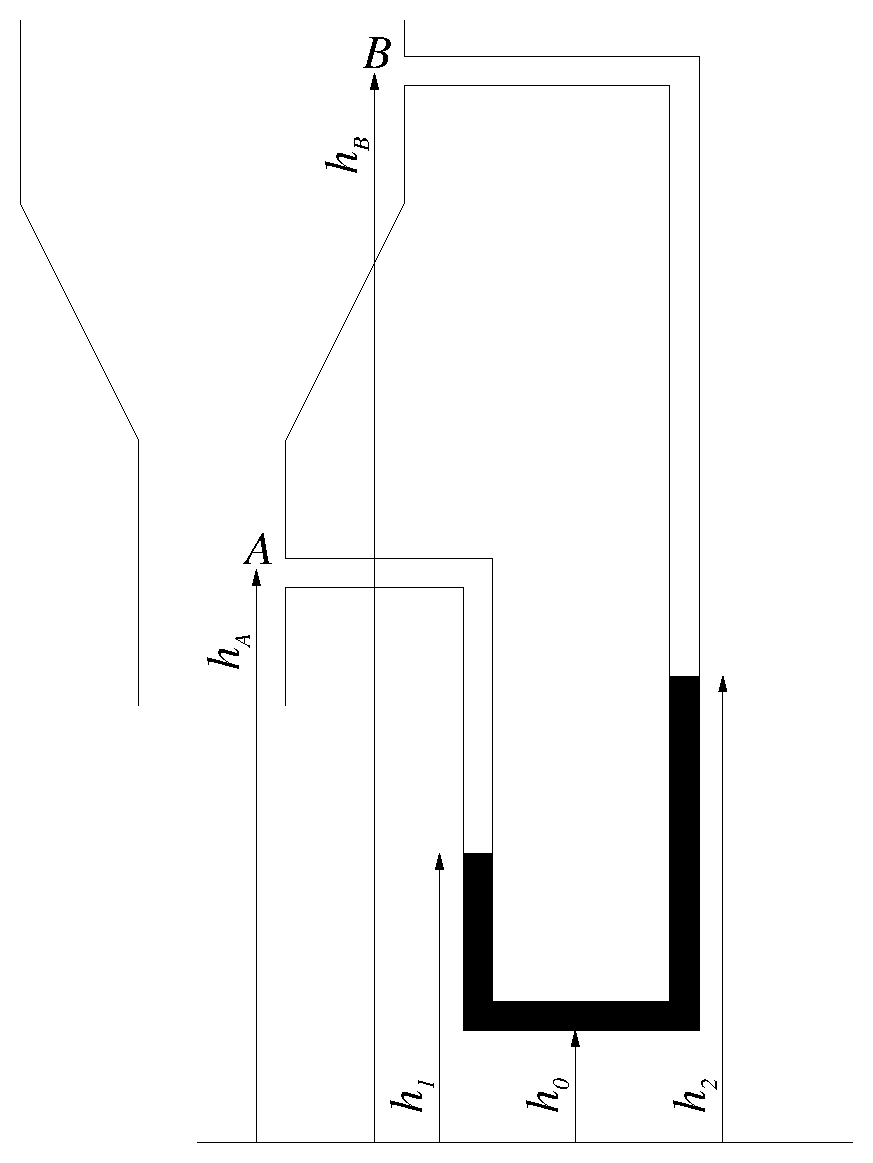
\includegraphics[width=0.90\textwidth]{./fig/manometro.eps}
   \end{center}
\end{minipage}
\end{tabular}

\sol

\partone Legge di Stevino. Manometro. Venturi.
%
\begin{equation}
   P_1 + \rho g h_1 = P_2 + \rho g h_2
\end{equation}

\parttwo
 Si scrive la legge di Stevino tra i punti A e 1, 1 e 2, 2 e B:
\begin{equation}\label{eqn:stevino:underdet}
\begin{cases}
  P_B + \rho_a g z_B = P_2 + \rho_a g z_2  \\
  P_1 + \rho g z_1 = P_2 + \rho g z_2   \\
  P_A + \rho_a g z_A = P_1 + \rho_a g z_1 \\
  \Delta P = P_B - P_A 
\end{cases}
\end{equation}
Si risolve il sistema lineare (come più piace). Ad esempio, partendo dalla terza e inserendo nella seconda e nella prima i risultati trovati:
\begin{equation}
\begin{aligned}
 & P_1 = P_A + \rho_a g (z_A - z_1) \\
 & P_2 = P_A + \rho_a g (z_A - z_1) + \rho g (z_1 - z_2) \\
 & P_B = P_A + \rho_a g (z_A - z_1) + \rho g (z_1 - z_2) + \rho_a g (z_2 - z_B)
\end{aligned}
\end{equation}
E quindi, portando $P_A$ a sinistra:
\begin{equation}
  \Delta P = -(\rho - \rho_a) g ( z_2-z_1) - \rho_a g (z_B - z_A) = -3909.8 Pa
\end{equation}

\paragraph{Osservazione.} Il sistema lineare (\ref{eqn:stevino:underdet}) è sotto determinato (se esiste una soluzione, ne esistono infinite), essendo un sistema lineare di 4 equazioni in 5 incognite, $P_1$, $P_2$, $P_A$, $P_B$, $\Delta P$. Il sistema lineare può essere scritto usando il formalismo matriciale come $\underline{\underline{A}}\,\underline{x} = \underline{b}$ con
\begin{equation}
 \underline{\underline{A}} = 
\begin{bmatrix}
  0 &  1 &  0 & -1 &  0 \\
  0 &  0 & -1 &  1 &  0 \\
 -1 &  1 &  1 &  0 &  0 \\
  1 & -1 &  1 &  0 &  0 \\
\end{bmatrix} , \quad
 \underline{x} = \begin{bmatrix}
  P_A \\ P_B \\ P_1 \\ P_2 \\ \Delta P
\end{bmatrix} , \quad
 \underline{b} = \begin{bmatrix}
  \rho_a g (h_2-h_B) \\ \rho g (h_1-h_2) \\ \rho_a g (h_A-h_1) \\ 0 
\end{bmatrix} \ .
\end{equation}
Poichè la matrice $\underline{\underline{A}}$ ha rango massimo (=\,4), esiste una soluzione $\underline{x}^*$ del problema, tale che  $\underline{\underline{A}}\,\underline{x}^* = \underline{b}$. Dal teorema del rango, si sa che il numero delle colonne (=\,5) di una matrice è uguale alla dimensione del suo rango (=\,4) e del suo nucleo (quindi =\,1). Il nucleo della matrice $\underline{\underline{A}}$, tutti i vettori $\underline{v}$ t.c.  $\underline{\underline{A}}\,\underline{v} = \underline{0}$, è uno spazio vettoriale di dimensione uno.
Se $\underline{x}^*$ è soluzione del sistema, allora anche tutti i vettori $\underline{x}^* + a \underline{v}$, $a \in \mathbb{R}$, sono soluzione del sistema, poichè $\underline{\underline{A}}(\underline{x}^* + \underline{v}) = \underline{\underline{A}}\,\underline{x}^* + \underline{\underline{A}}\,\underline{v} = \underline{b} + \underline{0}$.
 Si può dimostrare il nucleo di $\underline{\underline{A}}$ è generato dal vettore $\underline{v}=(1,1,1,1,0)^T$. Quindi le infinite soluzioni del problema hanno la forma
\begin{equation}
 \begin{bmatrix}
  P_A \\ P_B \\ P_1 \\ P_2 \\ \Delta P 
 \end{bmatrix} = 
 \begin{bmatrix}
  P_A^* \\ P_B^* \\ P_1^* \\ P_2^* \\ \Delta P 
 \end{bmatrix} + 
 \begin{bmatrix}
   a \\ a \\ a \\ a \\ 0
 \end{bmatrix} \ .
\end{equation}
Ora dovrebbe apparire chiaro come non sia possibile determinare il valore assoluto delle pressioni $P_1$, $P_2$, $P_A$, $P_B$ solamente da una misura di pressione con un manometro \textit{differenziale}: questi valori sono noti a meno di una costante additiva $a$, indeterminata. Al contrario, la differenza di due di questi valori, come $\Delta P = P_B - P_A$, è unica (e uguale al risultato ottenuto nello svolgimento del problema): l'unicità di $\Delta P$ dipende dalla forma dei vettori del nucleo di $\underline{\underline{A}}$ che hanno componente $\Delta P$ nulla.



 

\newpage

\cleardoublepage

% 02. tensione superficiale ------------
\chapterimage{blank_fig}
\chapter{Tensione superficiale}\index{Tensione superficiale}\label{ch:tensSup}

\paragraph{Legge di Young-Laplace.}
\begin{minipage}{0.60\textwidth}
La superficie di interfaccia tra due liquidi può essere modellata come una membrana, una superficie bidimensionale all'interno della quale agisce una forza per unità di lunghezza, tangente alla superficie stessa. La forza per unità di spessore $\gamma$ agente nella membrana viene definità \textit{tensione superificiale}. La legge di Young-Laplace lega la tensione superficiale, il salto di pressione attraverso la superficie di interfaccia e la curvatura della superficie stessa. Nel caso di tensione superficiale costante, vale
\begin{equation}
  p_b - p_a = \gamma \displaystyle\left( \frac{1}{R_1} + \frac{1}{R_2} \right) = 2 \gamma H
\end{equation}
 dove con $R_1$ e $R_2$ sono stati indicati i due raggi di curvatura della superficie e con $H$ si è indicata la curvatura media.
\end{minipage}
%
\begin{minipage}{0.40\textwidth}
  \begin{center}
    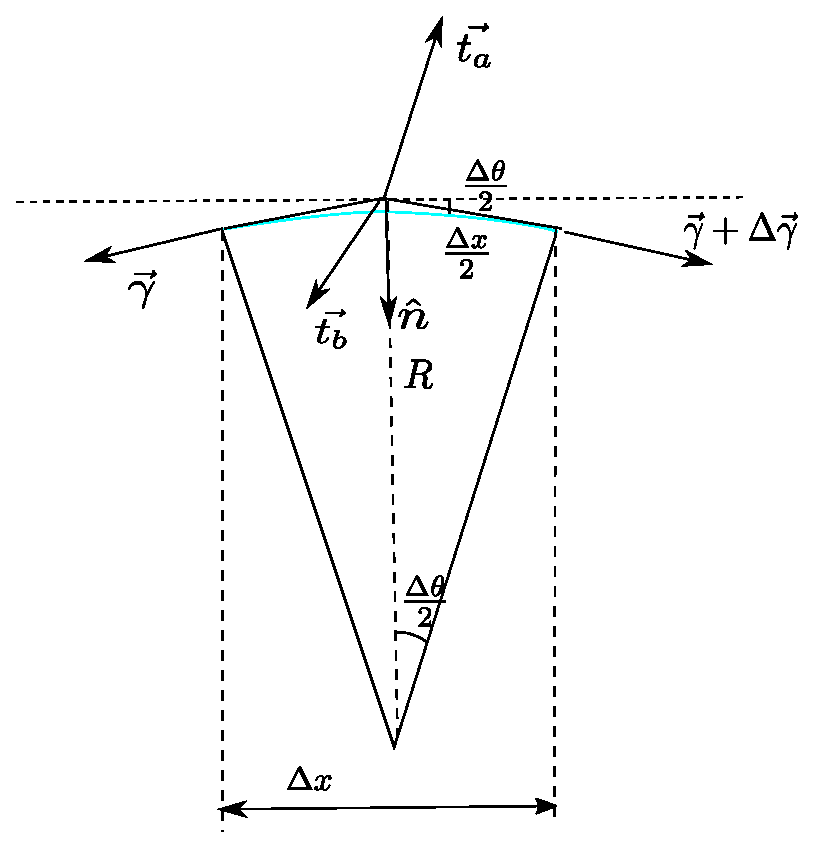
\includegraphics[width=0.95\textwidth]{./fig/laplaceYoung2Ddim.eps}
  \end{center}
\end{minipage}

\paragraph{Legge di Young-Laplace in due dimensioni.}
Viene ricavata la legge di Young-Laplace in due dimensioni, scrivendo l'equilibrio di un elemento di membrana (monodimensionale) soggetta agli sforzi esercitati dai due fluidi su di essa e alla tensione superficiale al suo interno. L'equazione vettoriale di equilibrio viene proiettata in direzione normale e tangente alla superficie. La superficie nell'intorno di un punto, viene approssimata come un arco infinitesimo di una circonferenza, come in figura.

Si considera un elemento infinitesimo di superficie di dimensioni $\Delta x \sim R \Delta \theta$. Anche l'angolo $\Delta \theta$ è ``piccolo'' ($\cos \Delta \theta \sim 1$, $\sin \Delta\theta \sim \Delta\theta$, la dimensione dell'elemento di superficie è approssimabile con la sua proiezione su un piano normale a $\bm{\hat{n}}$, ...). Con $R$ viene indicato il raggio di curvatura della superficie.

Si scrive l'equilibrio.
\begin{equation}
  \bm{t_a} \Delta x + \bm{t_b} \Delta x - \bm{\gamma}(x) + \bm{\gamma}(x) + \Delta \bm{\gamma} = 0
\end{equation}

Proiettando nelle direzioni normale e tangente alla superficie, 

\begin{equation}
 \begin{aligned}
  ( {t_a}_n + {t_b}_n )\Delta x + \gamma \sin \frac{\Delta\theta}{2}
      + (\gamma + \Delta \gamma) \sin \frac{\Delta\theta}{2} = 0 \\
  ( {t_a}_t + {t_b}_t )\Delta x - \gamma \cos \frac{\Delta\theta}{2}
      + (\gamma + \Delta \gamma) \cos\frac{\Delta \theta}{2} = 0
 \end{aligned}
\end{equation}

Inserendo i valori approssimati di $\sin \Delta \theta$ e $\cos \Delta \theta$, trascurando i termini di ordine superiore ($\Delta \gamma \Delta \theta$):

\begin{equation}
 \begin{aligned}
  & ( {t_a}_n + {t_b}_n )\Delta x + 2 \gamma \frac{\Delta \theta}{2} = 0 \\
  & ( {t_a}_t + {t_b}_t )\Delta x + \Delta \gamma = 0
 \end{aligned}
\end{equation}

Se si può confondere la coordinata che descrive la superficie con la coordinata $x$, si può 
approssimare $\Delta \gamma \sim \frac{\partial \gamma}{\partial x} \Delta x$.
Usando la relazione $\frac{\Delta x}{2} \sim R \frac{\Delta \theta}{2}$ e semplificando 
l'elemento $\Delta x$:

\begin{equation}\label{eqn:equil_young_laplace}
\begin{aligned}
 & ( {t_a}_n + {t_b}_n ) + \frac{\gamma}{R} = 0 \\
 & ( {t_a}_t + {t_b}_t ) + \frac{\partial \gamma}{\partial x} = 0
\end{aligned}
\end{equation}

Nel caso in cui si consideri un problema di statica, lo sforzo \textbf{sul} 
 fluido è dovuto solo al contributo di pressione, che agisce in direzione
 normale alla superficie: 
 $\bm{t}_a = -P_a \bm{\hat{n}_a}$,  $\bm{t}_b = -P_b \bm{\hat{n}_b}$. Lo
 sforzo che il fluido esercita sulla superficie di interfaccia è uguale
 in modulo e opposto in direzione. Le due
  normali sono tra di loro opposte: si sceglie di definire la normale
  $\bm{\hat{n}} = \bm{\hat{n}_a} = -\bm{\hat{n}_b}$. Di conseguenza, le
  componenti degli sforzi agenti sulla superficie di interfaccia, proiettati
  lungo $\bm{\hat{n}}$ e un versore tangente sono: ${{t_a}_n} = P_a$, 
  ${{t_b}_n} = - P_b$, ${{t_a}_t} = 0$, ${{t_b}_n} = 0$.
 Se $\gamma$ è costante (la tensione superficiale può avere gradienti non 
 nulli a causa di gradienti di temperatura o di concentrazione),
  l'equilibrio in direzione tangente è identicamente soddisfatto.

\begin{equation}
   P_a - P_b + \frac{\gamma}{R} = 0 \qquad 
  \Rightarrow  \qquad 
   P_b - P_a = \frac{\gamma}{R}
\end{equation}


\paragraph{Estensione al caso 3D.} Per estendere la dimostrazione al caso 3D, nel quale la superficie è 2D, si procede in modo analogo a quanto nel paragrafo precedente. Va considerata la curvatura di una superficie e non di una curva (esistono due raggi di curvatura), \dots Un utile primo riferimento di \textit{geometria differenziale} di curve e superfici, è disponibile in rete seguendo il collegamento

\vspace{0.3cm}
\noindent
\href{http://alpha.math.uga.edu/~shifrin/ShifrinDiffGeo.pdf}
 {Differential Geometry, Shiffrin}.

%\vspace{0.3cm}
%\noindent
%La formula che si ottiene, nel caso statico con $\gamma$ costante, è la seguente:
%\begin{equation}
%  p_b - p_a = \gamma \displaystyle\left( \frac{1}{R_1} + \frac{1}{R_2} \right) = 2 \gamma H
%\end{equation}
% dove con $H$ si è indicata la curvatura media.

\vspace{0.3cm}
\noindent
L'esistenza della tensione superificiale spiega il fenomeni della capillarità, l'esistenza dei menischi formati dalla superficie di separazione di due fluidi, il galleggiamento di insetti, graffette... sull'acqua, la formazione di superfici ``minimali'' di sapone, la bagnabilità delle superfici e la rottura di getti di piccolo diametro e la formazione di gocce. Infine, può essere utilizzata anche come mezzo non convenzionale di propulsione per barchette di carta

\vspace{0.3cm}
\noindent
\href{https://www.youtube.com/watch?v=Oz54Auev9eU}{Boat without a motor - Marangoni effect}

\clearpage
\noindent
\begin{tabular}{cc}
\begin{minipage}[b]{0.65\textwidth}
\begin{exerciseS}[Capillare]
Sia $\theta$ l'angolo di contatto all'interfaccia tra aria, liquido e solido; 
sia $\gamma$ la tensione superficiale tra aria e liquido; sia $\rho$ la densità del liquido.
Determinare l'altezza $h$ dal liquido in una colonnina cilindrica di raggio $r = 0.5 \ mm$  rispetto al livello
nella vasca. Calcolare poi la pressione all'interno della colonnina.
(Si può considerare valida l'approssimazione che la pressione agente sulla vasca e sulla superficie
superiore del liquido all'interno della colonnina sia uguale).

\vspace{0.1cm}
Si considerino condizioni termodinamiche e materiale della colonnina tali che:
se il liquido è acqua: $\rho = 999 \ kg/m^3$, $\theta={1}\degree$, $\gamma=0.073 N/m$.
se il liquido è mercurio: $\rho = 13579 \ kg/m^3$, $\theta={140}\degree$, $\gamma=0.559 N/m$.
($h_{H_2O} = 2.97 \ cm$, $P_{H_20} - P_0 =  - 291.95 \ Pa$; $h_{Hg} = -1.28 \ cm$, $P_{Hg} - P_0 =  1712.87 \ Pa$)
\end{exerciseS}
\end{minipage}
&
\begin{minipage}[b]{0.35\textwidth}
   \begin{center}
   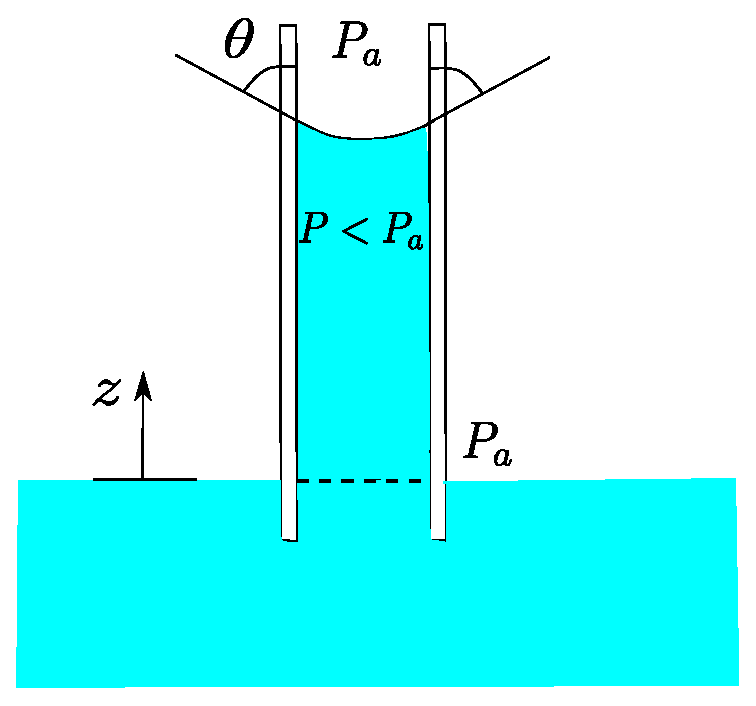
\includegraphics[width=0.80\textwidth]{./fig/cap01.eps}
   \end{center}
\end{minipage}
\end{tabular}

\sol

\partone
 Tensione superficiale. Angolo di contatto. Capillarità. Menisco.

\parttwo
 Scrivendo l'equilibrio per il volume di fluido nel capillare si trova l'altezza $h$.
Successivamente si trova la $p$ usando la legge di Stevino. Infine si fanno osservazioni su angolo di contatto,
menisco e salto di pressione all'interfaccia.
%
\begin{itemize}
\item Si scrive l'equilibrio del volume di fluido. Il problema è di statica. Le forze agenti sono la forza
dovuta alla tensione superficiale (che agisce sul perimetro della superficie superiore) e la forza peso, poichè per ipotesi la pressione agente sulla superficie superiore è uguale alla pressione ambiente $P_a$; e quindi??? Perchè la componente verticale della risultante dovuta alla pressione esterna è zero??? Vedere immagine...).
%
\begin{equation}
  F_{\gamma} = F_g \quad \Rightarrow \quad 2\pi r \gamma  \cos \theta = \pi r^2 h \rho g
\end{equation}
%
E quindi: 
\begin{equation}
  h = \frac{2 \gamma \cos \theta}{\rho g r}
  \quad \Rightarrow \quad
  \begin{cases}
    h_{H_20} = 2.97 \ cm \\
    h_{Hg} = -1.28 \ cm
  \end{cases}
\end{equation}
%
\textit{Commenti sul risultato.} L'effetto della capillarità è più evidente per tubi stretti (proporzionalità con $1/r$). La quota $h$ può assumere sia valori positivi, sia valori negativi, 
in base al valore dell'angolo di contatto: $h \le 0$, per $\theta \ge \pi/2$.
%
%\begin{figure}[h]
%\centering
%\captionsetup[subfigure]{labelformat=empty}
%\subfloat[][\emph Equilibrio del volume di fluido nella colonnina. La pressione atmosferica $P_a$ non
%   influenza l'equilibrio. Perchè?]
%   {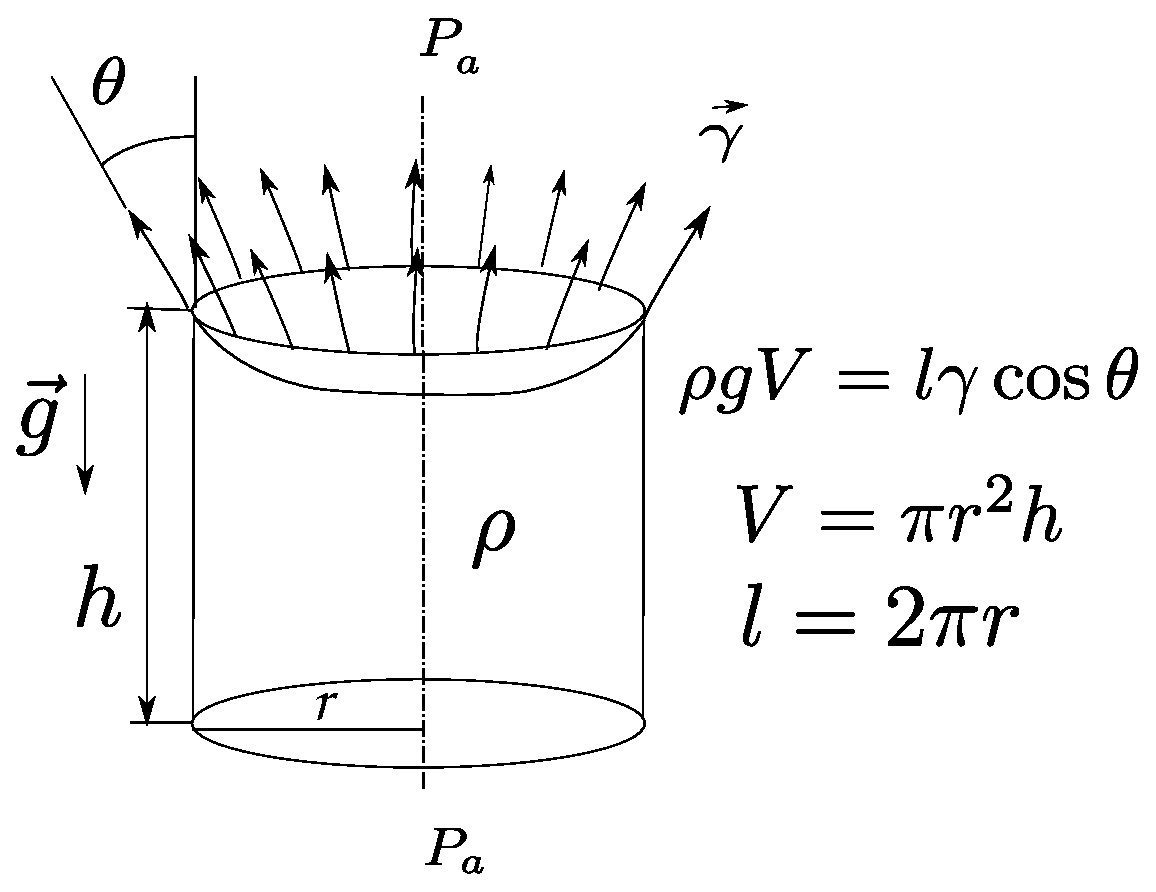
\includegraphics[width=0.30\textwidth]{./fig/equil.eps}}
%\end{figure}
%
\item Si calcola la pressione nel fluido in cima alla colonnina sfruttando la legge di Stevino.
\begin{equation}
  P = P_0 - \rho g h = P_0 - \frac{2 \gamma \cos \theta}{r}
  \quad \Rightarrow \quad
  \begin{cases}
    P_{H_20} - P_0 =  - 291.95 \ Pa \\
    P_{Hg}   - P_0 =  1712.87 \ Pa
  \end{cases}
\end{equation}
%
\textit{Commenti sul risultato.}  $P-P_0 \le 0$, per $\theta \le \pi/2$. Al contrario $P-P_0 \ge 0$, per $\theta \ge \pi/2$. Questi risultati sono compatibili (meno male) con le relazioni tra curvatura (stretta parente del menisco e dell'angolo di contatto) e il salto di pressione.
%
\begin{center}
  \begin{tabular}{ c c c }
    \hline
    $\theta \le \pi/2$ & $h \ge 0$  & $P \le P_a$ \\ \hline
    $\theta \ge \pi/2$ & $h \le 0$  & $P \ge P_a$ \\ \hline
  \end{tabular}
\end{center}

\begin{figure}
\centering
%\captionsetup[subfigure]{labelformat=empty}
\subfloat[][\emph Differenza tra il menisco formato dall'acqua e dal mercurio 
    con aria e solido (quale?): diversa concavità della superficie. ]
   {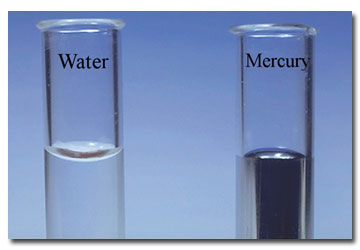
\includegraphics[width=0.32\textwidth]{./fig/menisco.jpg}} \quad
\subfloat[][\emph Rappresentazione del caso del problema in cui il liquido è mercurio: 
    l'angolo di contatto è maggiore dell'angolo retto, la quota all'interno del capillare
    è minore di quella nella vasca. Il caso dell'acqua è rappresentato a finaco del testo del problema.]
   {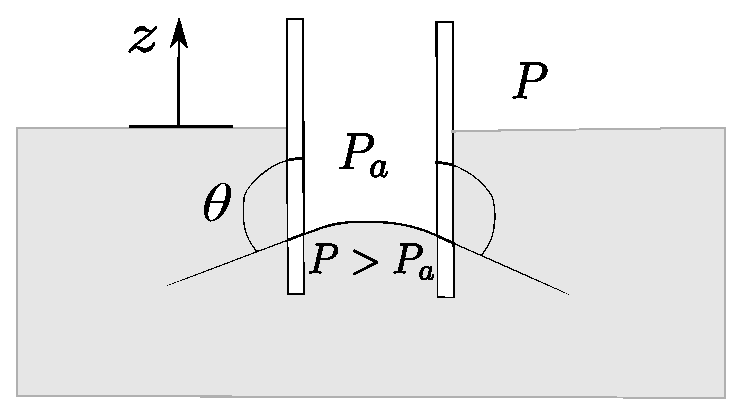
\includegraphics[width=0.32\textwidth]{./fig/cap02.eps}} \quad
%\subfloat[][\emph Rappresentazione delle condizioni all'interfaccia tra due fluidi quando viene considerato il contributo della tensione superficiale: secondo la formula di Young-Laplace vale $\bm{t_A} - \bm{t_B} = \gamma \bm{\hat{n}} (\frac{1}{R_1} + \frac{1}{R_2})$, dove $\bm{\hat{n}}$ è la normale e $R_1$, $R_2$ sono i raggi di curvatura della superficie. ]
%   {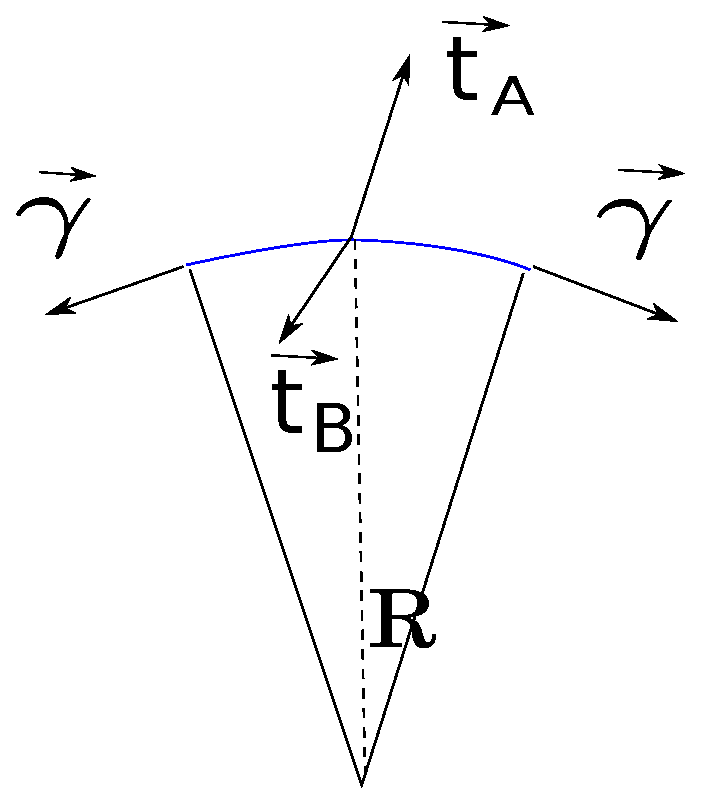
\includegraphics[width=0.22\textwidth]{./fig/laplaceYoung2D.eps}}
\subfloat[][\emph Equilibrio del volume di fluido nella colonnina. La pressione atmosferica $P_a$ non
   influenza l'equilibrio. Perchè?]
   {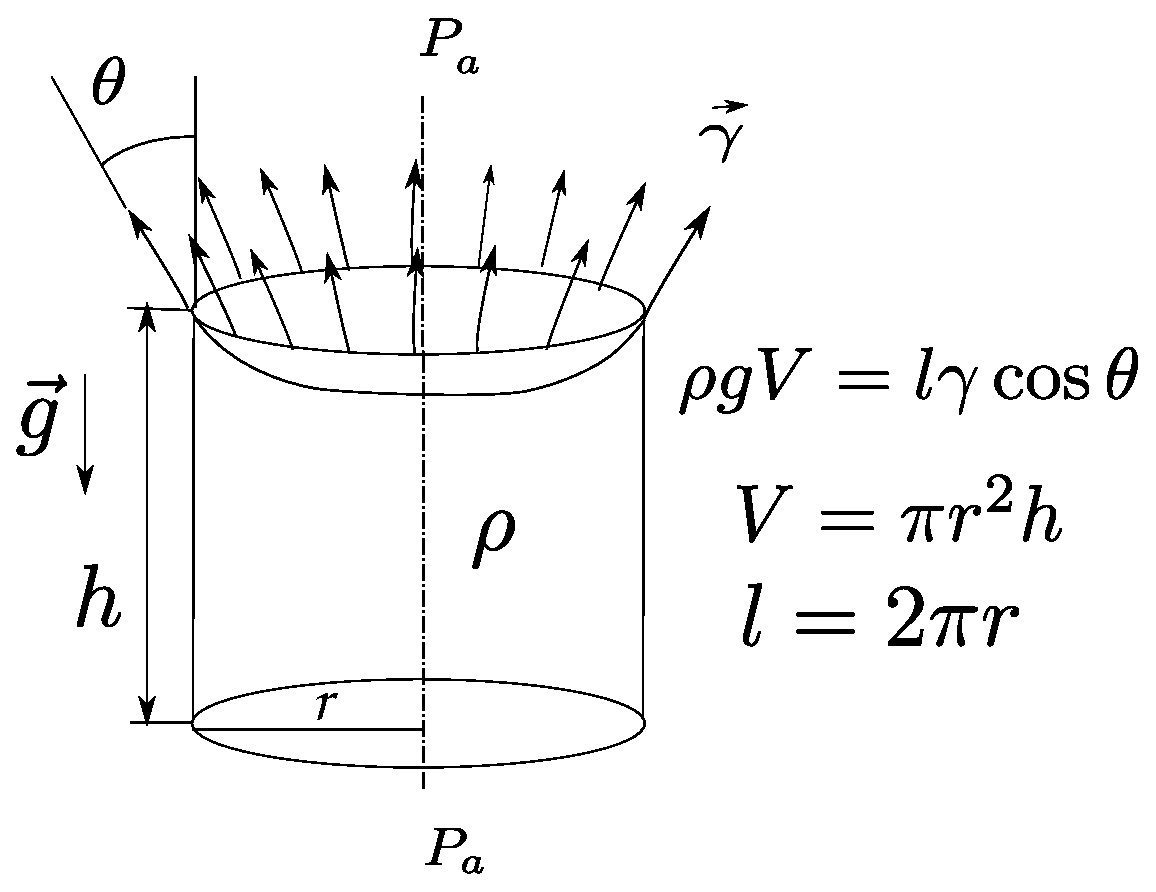
\includegraphics[width=0.30\textwidth]{./fig/equil.eps}}
\end{figure}


\end{itemize}











\clearpage
\noindent
\begin{tabular}{cc}
\begin{minipage}[b]{0.60\textwidth}
\begin{exerciseS}[Attrazione di due superfici]
Due lamine piane uguali parallele sono separate da una distanza $d$. Tra le lamine è 
presente un sottile strato di liquido. Sono note l'area della superficie $A$ e il perimetro $L$ delle due lamine,
la pressione ambiente $p_a$, la tensione superficiale del liquido $\gamma$ e l'angolo di contatto $\theta$.
Si chiede di determinare la componente perpendicolare alle lamine della forza agente su ciascuna delle due lamine.
\end{exerciseS}
\end{minipage}
&
\begin{minipage}{0.35\textwidth}
   \begin{center}
   \includegraphics[width=0.85\textwidth]{./fig/Plates4}
   \end{center}
\end{minipage}
\end{tabular}

\sol

\partone
 Tensione superficiale. Angolo di contatto.

\parttwo
 La condizione descritta nell'esercizio è una condizione equilibrio. La forza agente su una lamina
è dovuta a due fenomeni: la tensione superficiale sul perimetro del fluido e la differenza di pressione tra fluido 
e ambiente. Si consideri positiva la forza se è una forza di attrazione.

\begin{equation}
  F = F_\gamma + F_p
\end{equation}

\begin{itemize}
  \item Calcolo di $F_\gamma$.
    \begin{equation}
     F_\gamma = \gamma L \sin\gamma
    \end{equation}
  
  \item Calcolo di $F_p$. Il salto di pressione viene calcolato scrivendo l'equilibrio all'interfaccia.
    \begin{equation}
     F_p = (p_a - p) A
    \end{equation}
    con:
    \begin{equation}
     (p_a - p) d = 2 \gamma \cos \theta
    \end{equation}
   
    
  \item La componente totale richiesta risulta quindi:
  \begin{equation}
    F = \frac{2 \gamma A \cos \theta}{d} + L \gamma \sin \theta
  \end{equation}
  
  \begin{center}
     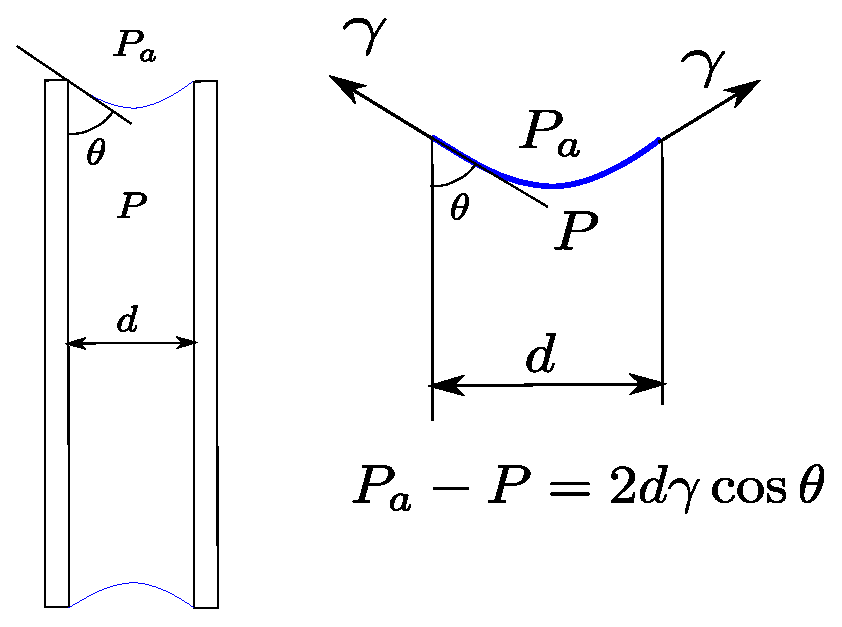
\includegraphics[width=0.50\textwidth]{./fig/sup01.eps}
   \end{center}
     
\end{itemize}

\clearpage

\cleardoublepage

% 03. cinematica -----------------------
\chapterimage{blank_fig}
\chapter{Cinematica}\index{Cinematica}\label{ch:cinematica}

La cinematica è la parte della meccanica che studia il moto di sistemi, indipendentemente dalle cause che lo generano, a differenza della dinamica. Prima di ricavare le equazioni che descrivono la dinamica di un fluido, sembra quindi opportuno concentrarsi sulla sua cinematica.

La cinematica e la dinamica dei mezzi continui, come ad esempio i solidi o i fluidi, possono essere descritte con un approccio lagrangiano o euleriano. La \textbf{descrizione lagrangiana}, utilizzata spesso in meccanica dei solidi, consiste nel seguire nello spazio il moto delle singole particelle del mezzo continuo. La \textbf{descrizione euleriana}, utilizzata spesso in meccanica dei fluidi, consiste nel descrivere l'evoluzione del mezzo continuo utilizzando come variabili indipendenti sia la variabile spaziale $\bm{r}$ sia la variabile temporale $t$.


\section{Descrizione integrale lagrangiana ed euleriana}

In una descrizione \textit{integrale} del fenomeno, l'approccio lagrangiano segue l'evoluzione di un \textbf{volume materiale}, i cui punti si muovono in maniera solidale con il mezzo continuo. In un approccio euleriano invece viene introdotto un \textbf{volume di controllo}, fisso nello spazio, e i flussi delle quantità meccaniche  (massa, quantità di moto, energia, \dots) contribuiscono ai bilancio delle quantità meccaniche relative al volume di controllo considerato. Queste due descrizioni sono casi particolari di un approccio generale al problema, definito \textit{ALE} (arbitrario lagrangiano-euleriano), che descrive l'evoluzione di un volume in moto arbitrario.
\newline
Le tre diverse descrizioni del problema possono essere messe in relazione tra di loro, tramite le formule di Leibniz, che forniscono l'espressione della derivata temporale di integrali su domini dipendenti dal tempo. Si riporta qui, senza dimostrazione, il \textbf{teorema del trasporto di Reynolds}
\begin{fBox}
\begin{equation}
 \dfrac{d}{d t} \int_{V(t)} f = \int_{V(t)} \dfrac{\partial f}{\partial t} +
  \oint_{S(t)} f\bm{v} \cdot \bm{\hat{n}} \ , 
\end{equation}
\end{fBox}
 che fornisce l'espressione della derivata temporale dell'integrale della funzione $f(\bm{x},t)$ (che può essere scalare, vettoriale o in generale tensoriale) nel volume mobile $V(t) \ni \bm{x}$, la cui frontiera $S(t)$ si muove con velocità $\bm{v}(\bm{x}_s,t)$, $\bm{x}_s \in S(t)$. La normale $\bm{\hat{n}}$ alla superficie $S(t)$ è uscente dal volume $V(t)$. 
%\newline 
Si rimanda all'appendice ``Richiami di analisi'' per la dimostrazione del teorema e per le formule della derivata temporale di flussi e circuitazioni su domini dipendenti dal tempo.
\newline
Siano ora
\begin{itemize}
 \item $V(t)$ un volume materiale, la cui frontiera si muove con la velocità del fluido $\bm{v}=\bm{u}$
 \item $V_c$ un volume di controllo, la cui frontiera è fissa nello spazio, $\bm{v}=\bm{0}$
 \item $v(t)$ un volume in moto arbitrario, la cui frontiera si muove con velocità generica $\bm{v}$.
\end{itemize}
Come si vedrà nel capitolo sui ``Bilanci integrali'', il bilancio integrale di una quantità meccanica $f$ in un volume materiale $V(t)$ descrive la variazione nel tempo dell'integrale $\int_{V(t)} f$. Il teorema di Reynolds applicato all'integrale svolto su un volume materiale $V(t)$ e all'integrale svolto sul volume in moto generico $v(t)$, coincidente con $V(t)$ all'istante di tempo $t$ considerato,
\begin{equation}
\begin{aligned}
  \dfrac{d}{d t} \int_{V(t)} f & = \int_{V(t)} \dfrac{\partial f}{\partial t} +
  \oint_{S(t)} f\bm{u} \cdot \bm{\hat{n}}  \\
  \dfrac{d}{d t} \int_{v(t)\equiv V(t)} f & = \int_{v(t)\equiv V(t)} \dfrac{\partial f}{\partial t} +
  \oint_{s(t)\equiv S(t)} f\bm{v} \cdot \bm{\hat{n}}  \ , \\
\end{aligned}
\end{equation}
permette di ricavare il legame tra la descrizione lagrangiana e una descrizione arbitraria del problema. Confrontando le ultime due espressioni, si ottiene
\begin{fBox}
\begin{equation}
 \dfrac{d}{d t} \int_{V(t)} f = \dfrac{d}{d t} \int_{v(t)\equiv V(t)} f +
 \oint_{s(t)\equiv S(t)} f (\bm{u} - \bm{v}) \cdot \bm{\hat{n}} \ . 
\end{equation}
\end{fBox}
Dalla formula scritta per il volume arbitrario $v(t)$, si ricava il legame tra a descrizione lagrangiana e la descrizione euleriana del problema, considerando il volume arbitrario coincidente con un volume di controllo $V_c$ fisso, per il quale $\bm{v}=\bm{0}$,
\begin{fBox}
\begin{equation}
 \dfrac{d}{d t} \int_{V(t)} f = \dfrac{d}{d t} \int_{V_c\equiv V(t)} f +
 \oint_{S_c\equiv S(t)} f \bm{u} \cdot \bm{\hat{n}} \ .
\end{equation}
\end{fBox}

\section{Descrizione puntuale lagrangiana ed euleriana}

% fissare un volume di controllo e descrivere la variazione delle quantità meccaniche al suo interno, tenendo in considerazione i flussi della quantità meccanica attraverso le pareti fisse del volume di controllo.
%\'E possibile descrivere l'evoluzione delle quantità meccaniche di particelle e volumi in moto arbitrario, come si vedrà in \S.

In una descrizione \textit{puntuale} del fenomeno, vengono introdotti due sistemi di coordinate: uno è solidale con il mezzo continuo dipendente dal tempo, mentre l'altro è fisso. 
Si può pensare al sistema di riferimento solidale con il continuo come un' ``etichetta'' che viene applicata a ogni \textbf{punto materiale} del mezzo continuo stesso. Un sistema di riferimento fisso, invece, è indipendente dal moto del mezzo continuo, come ad esempio un sistema di coordinate cartesiane, la cui origine e i cui assi sono fissi nel tempo.
%
Mentre il mezzo continuo evolve nel tempo (trasla, ruota, si deforma \dots), un punto materiale ha coordinate costanti $\bm{x_0}$ rispetto al sistema di riferimento ``solidale al volume'', cioè che si muove e si deforma insieme al volume: questa coordinata, detta lagrangiana, può essere pensata come l'``etichetta'' assegnata al punto materiale del continuo. Le coordinate euleriane $\bm{x}(\bm{x_0},t)$ del punto materiale con coordinate lagrangiane $\bm{x_0}$, ne descrivono il moto nel sistema di riferimento fisso e in generale sono una funzione del tempo
%
\begin{remark}
 Il sistema di riferimento solidale al corpo dipende dal tempo, mentre le coordinate lagrangiane $\bm{x_0}$ di un punto materiale sono costanti.
 Il sistema di riferimento fisso è indipendente dal tempo, mentre le coordinate euleriane $\bm{x}$ di un punto materiale del volume (quindi con $\bm{x_0}$ costante) sono dipendenti dal tempo.
\end{remark}
% 
Assumendo che all'istante $t=0$ i due sistemi di coordinate coincidano, e che quindi coincidano anche le coordinate euleriane e lagrangiane $\bm{x}(\bm{x_0},0) = \bm{x_0}$, le coordinate lagrangiane $\bm{x_0}$ rappresentano la configurazione (iniziale) di riferimento della configurazione attuale $\bm{x}(\bm{x_0},t)$. La trasformazione $\bm{x}(\bm{x_0},t)$ descrive l'evoluzione nel tempo $t$ dei punti $\bm{x}(0) = \bm{x_0}$ appartenenti al volume $V_0 = V(0)$, all'istante iniziale. La velocità $\bm{u}(\bm{x},t)$ del mezzo continuo nel punto $\bm{x}(\bm{x_0},t)$, per definizione di punto materiale, coincide con la velocità $\bm{u_0}(\bm{x_0},t)$ del punto etichettato con $\bm{x_0}$: questa è la derivata nel tempo della sua posizione $\bm{x}$, cioè con la derivata nel tempo della mappa $\bm{x}(\bm{x_0},t)$ a coordinata lagrangiana (che identifica la particella) costante,
 \begin{equation}
  \bm{u_0}(\bm{x_0},t) = \dfrac{\partial \bm{x}}{\partial t}\bigg|_{\bm{x_0}}(\bm{x_0},t) =: \dfrac{d \bm{x}}{d t}(\bm{x_0},t) =: \dfrac{D\bm{x}}{D t}(\bm{x_0},t) \ ,
 \end{equation}
dove è stato introdotto il simbolo $D/Dt$ di \textbf{derivata materiale} che rappresenta l'evoluzione della quantità alla quale è applicata, seguendo il moto del mezzo continuo: la derivata materiale rappresenta la variazione nel tempo della quantità ``sentita'' dalle singole particelle materiali.
%
 Nella descrizione euleriana del problema, i campi sono funzioni delle variabili indipendenti spazio $\bm{x}$ e tempo $t$. Data una funzione $f(\bm{x},t)$ (scalare, vettoriale, tensoriale), viene indicata con
 \begin{equation}
 \dfrac{\partial f}{\partial t} = \dfrac{\partial f}{\partial t}\bigg|_{\bm{x}}(\bm{x},t) \ ,
 \end{equation}
 la derivata parziale rispetto al tempo, che rappresenta la variazione della quantità $f(\bm{x},t)$ nel punto fisso $\bm{x}$ dello spazio, che coordinata euleriana costante.

%Si riporta poi per completezza e per dare un'interpretazione anche la definizione di $\dfrac{d f}{d t}$, già usata sopra nella
% definizione della velocità di un punto del volume
% \begin{equation}
%  \dfrac{d f}{d t} = \dfrac{\partial f}{\partial t}\bigg|_{\bm{x_0}}
% \end{equation}
%che viene svolta a $\bm{x_0}$ costante: questa derivata temporale è quella che consente di considerare la variazione
% della funzione $f$, percepita dal punto etichettato $\bm{x_0}$ che evolve con il volume.
%%
\'E possibile trovare il legame tra le due derivate utilizzando la \textit{regola di derivazione di funzioni composte} e la funzione $\bm{x}(\bm{x_0},t)$ che descrive il moto dei punti materiali del sistema.
Data una funzione $f(\bm{x},t)$ (rappresentazione euleriana), viene definita $f_0(\bm{x_0},t)$ come la funzione composta $f_0 = f \circ \bm{x}$ (descrizione lagrangiana). Ipotizzando poi che si possano esprimere le coordinate lagrangiane come funzione di quelle euleriane, $\bm{x_0}(\bm{x},t)$, è possibile scrivere
\begin{equation}
 f(\bm{x},t) = f(\bm{x}(\bm{x_0},t),t) = f_0(\bm{x}_0,t) = f_0(\bm{x_0}(\bm{x},t),t) \ .
\end{equation}
Utilizzando la regola di derivazione per le funzioni composte, si ottiene il legame cercato,
\begin{equation}\label{eqn:cin:lagr-eul}
\begin{aligned}
 \dfrac{D f}{D t}(\bm{x},t) & = \dfrac{\partial f}{\partial t}\bigg|_{\bm{x_0}} = \dfrac{\partial}{\partial t}\bigg|_{\bm{x_0}} f(\bm{x}(\bm{x_0},t),t) =  \\ 
  & = \dfrac{\partial f}{\partial \bm{x}}\bigg|_{t} \cdot \dfrac{\partial \bm{x}}{\partial t}\bigg|_{\bm{x_0}} 
  + \dfrac{\partial f}{\partial t}\bigg|_{\bm{x}} = 
  \dfrac{\partial f}{\partial t} +  
  \dfrac{\partial x_i}{\partial t}\bigg|_{\bm{x_0}} \dfrac{\partial f}{\partial x_i}\bigg|_{t}  = 
  \dfrac{\partial f}{\partial t} + \bm{u} \cdot \bm{\nabla} f \ ,
\end{aligned}
\end{equation}
dove si è indicato con $\bm{u}(\bm{x},t) = \dfrac{\partial \bm{x}}{\partial t}\bigg|_{\bm{x_0}} (\bm{x_0}(\bm{x},t),t)$ il campo di velocità riferito a una descrizione euleriana del problema e si è riconosciuto l'operatore $\bm{\nabla}$ nell'ultimo passaggio. Infine è possibile ``rimuovere'' la funzione $f$ per ottenere la relazione tra la forma delle due derivate, valida per funzioni scalari, vettoriali, tensoriali,
\begin{fBox}
\begin{equation}\label{eqn:cin:lagr-eul}
 \dfrac{D \rule{1.5ex}{.4pt}}{D t} := \dfrac{d \rule{1.5ex}{.4pt}}{d t} := \dfrac{\partial \rule{1.5ex}{.4pt}}{\partial t}\bigg|_{\bm{x_0}} = \dfrac{\partial \rule{1.5ex}{.4pt}}{\partial t} + \bm{u} \cdot \bm{\nabla} \rule{1.5ex}{.4pt} \ .
\end{equation}
\end{fBox}

Come esempio, applichiamo la regola (\ref{eqn:cin:lagr-eul}) per ricavare la forma euleriana e lagrangiana del campo di velocità e di accelerazione delle particelle del continuo. Il campo di velocità $\bm{u}(\bm{x},t)$ si ottiene dalla derivata materiale della trasformazione $\bm{x}(x_0,t)$,
\begin{equation}
 \bm{u}(\bm{x},t) = \dfrac{D \bm{x}}{D t} = \underbrace{\dfrac{\partial \bm{x}}{\partial t}\bigg|_{\bm{x}} }_{=0} + \bm{u_0}(\bm{x_0},t) \cdot \underbrace{ \bm{\nabla} \bm{x} }_{=\mathbb{I}} =
 \bm{u_0}(\bm{x_0},t) \ .
\end{equation}
In questo caso, non è stato ottenuto nulla di nuovo. Il campo di accelerazione nella descrizione euleriana del fenomeno viene ottenuto calcolando l'accelerazione delle particelle materiali con la derivata materiale alla velocità. Per componenti, l'accelerazione della particella materiale identificata con $\bm{x_0}$ è
\begin{equation}
 a_{i}(\bm{x},t) = \dfrac{D u_{i}}{D t} = 
 \dfrac{\partial u_i}{\partial t} + u_{k} \dfrac{\partial u_i}{\partial x_k} \ .
\end{equation}
Introducendo l'operatore advettivo $\bm{v}\cdot \bm{\nabla}$, è possibile scrivere il campo di accelerazione (che comparirà nel bilancio della quantità di moto) in forma vettoriale
\begin{equation}
 \bm{a}(\bm{x},t) = \dfrac{D \bm{u}}{D t}(\bm{x},t) = \dfrac{\partial \bm{u}}{\partial t}(\bm{x},t) + (\bm{u}(\bm{x},t) \cdot \bm{\nabla}) \bm{u}(\bm{x},t) \ ,
\end{equation}
dove sono stati esplicitati gli argomenti $(\bm{x},t)$ delle funzioni, per evidenziare la rappresentazione euleriana. 

\begin{remark}
 Una volta compresa la differenza tra le due descrizioni del problema, non è necessario esprimere in maniera esplicita gli argomenti delle funzioni. Da qui in avanti, verrà privilegiata una descrizione euleriana, per campi, del problema.
\end{remark}
%
In alcuni casi, come ad esempio problemi che riguardano lo studio di correnti attorno a corpi mobili, può essere conveniente utilizzare una rappresentazione arbitraria del problema, descrivendo il fenomeno seguendo l'evoluzione delle grandezza meccaniche su punti, ``etichettati'' dalla coordinata arbitraria $\bm{\chi}$, il cui moto è descritto in coordinate euleriane dalla funzione $\bm{x}(\bm{\chi},t)$. Seguendo lo stesso procedimento svolto per le particelle materiali, la velocità $\bm{v}$ di questi punti in moto arbitrario è uguale alla derivata parziale
\begin{equation}
 \bm{v} = \dfrac{\partial \bm{x}}{\partial t} \bigg|_{\bm{\chi}} \ ,
\end{equation}
svolta a coordinata $\bm{\chi}$ costante. Ancora seguendo lo stesso procedimento svolto in precedenza, è possibile ricavare la relazione tra la rappresentazione arbitraria e quella euleriana,
\begin{fBox}
\begin{equation}\label{eqn:cin:ale-eul}
 \dfrac{\partial \rule{1.5ex}{.4pt}}{\partial t} \bigg|_{\bm{\chi}} = \dfrac{\partial \rule{1.5ex}{.4pt}}{\partial t} \bigg|_{\bm{x}} + \bm{v} \cdot \bm{\nabla} \rule{1.5ex}{.4pt} \ .
\end{equation}
\end{fBox}
e, confrontando la (\ref{eqn:cin:lagr-eul}) e la (\ref{eqn:cin:ale-eul}), la relazione tra la rappresentazione arbitraria e quella lagrangiana,
\begin{fBox}
\begin{equation}
  \dfrac{\partial \rule{1.5ex}{.4pt}}{\partial t} \bigg|_{\bm{x_0}} = \dfrac{\partial \rule{1.5ex}{.4pt}}{\partial t} \bigg|_{\bm{\chi}} + (\bm{u} - \bm{v}) \cdot \bm{\nabla} \rule{1.5ex}{.4pt} \ .
\end{equation}
\end{fBox}

\section{Velocità di traslazione, rotazione e deformazione}
In questa sezione viene studiato il moto di un segmento materiale, che segue il moto del mezzo continuo. Viene introdotto il tensore gradiente di velocità $\bm{\nabla}\bm{u}$, con $\bm{u}(\bm{x},t)$ il campo di velocità. Questo tensore viene prima scritto come somma della sua parte antisimmetrica $\mathbb{W}$ e della sua parte simmetrica $\mathbb{D}$, la quale può essere a sua volta scomposta nella parte idrostatica e nella parte deviatorica $\mathbb{D}^d$. Viene infine descritta la natura di questi tensori grazie alla loro influenza sul moto di segmento materiale. 

Il segmento materiale viene identificato dal vettore $\Delta\bm{x_{12}}(t) = \bm{x_2}(t) - \bm{x_1}(t)$, i cui estremi sono i punti di coordinate $\bm{x_1}(t)$ e $\bm{x_2}(t)$. Indicando con $\bm{u_1}(t) = \bm{u}(\bm{x_1}(t),t)$ e $\bm{u_2}(t) = \bm{u}(\bm{x_2}(t),t)$ loro velocità, è possibile ricavare l'evoluzione temporale del segmento materiale,
\begin{equation}
 \Delta\bm{x_{12}}(t+\Delta t) = \Delta\bm{x_{12}}(t) + \left( \bm{u_2}(t) - \bm{u_1}(t) \right) \Delta t + o(\Delta t) \ .
\end{equation}
Tornando alla descrizione euleriana del problema, è possibile scrivere la differenza di velocità introducendo il tensore gradiente di velocità,
\begin{equation}
\begin{aligned}
 \bm{u_2}(t) - \bm{u_1}(t) & = \bm{u}(\bm{x_2}(t),t) - \bm{u}(\bm{x_1}(t),t) = \\
 & = \bm{u}\left(\bm{x_1}(t)+\Delta\bm{x_{12}}(t),t\right) - \bm{u}\left(\bm{x_1}(t),t\right) = \\
 & = \bm{u}\left(\bm{x_1}(t),t\right) + \bm{\nabla}\bm{u}\left(\bm{x_1}(t),t\right) \cdot \Delta\bm{x_{12}}(t) - \bm{u}\left(\bm{x_1}(t),t\right) + o(|\Delta\bm{x_{12}}(t)|) = \\
 & = \bm{\nabla}\bm{u}\left(\bm{x_1}(t),t\right) \cdot \Delta\bm{x_{12}}(t) + o(|\Delta\bm{x_{12}}(t)|) \ . \\
 \end{aligned}
\end{equation}
Riarrangiando i termini si può scrivere,
\begin{equation}\label{eqn:cin:material-segm}
 \Delta\bm{x_{12}}(t+\Delta t) = \Delta\bm{x_{12}}(t) + 
 \big[ \bm{\nabla}\bm{u}\left(\bm{x_1}(t),t\right) \cdot \Delta\bm{x_{12}}(t) + o(|\Delta\bm{x_{12}}(t)|) \big] \Delta t + o(\Delta t) \ .
\end{equation}
e facendo tendere a zero $\Delta t$, si ricava
\begin{equation}
 \dfrac{d \Delta\bm{x_{12}}}{d t}(t) = \bm{\nabla}\bm{u}\left(\bm{x_1}(t),t\right) \cdot \Delta\bm{x_{12}}(t) + o(|\Delta\bm{x_{12}}(t)|) \ .
\end{equation}
%
Nell'ipotesi che i termini $o(|\Delta \bm{x_{12}}(t)|)$ siano trascurabili, la velocità $\bm{u_2}$ del punto $\bm{x_2}$ differisce dalla velocità $\bm{u_1}$ del punto $\bm{x_1}$ del termine $d \Delta\bm{x_{12}}/d t$ che rappresenta le eventuali rotazioni rigide e le deformazioni del mezzo continuo,
\begin{equation}\label{eqn:cin:relative-vel-1}
 \bm{u_2}(t) = \bm{u_1}(t) + \bm{\nabla}\bm{u}\left(\bm{x_1}(t),t\right) \cdot \Delta\bm{x_{12}}(t) \ .
\end{equation}
 
\subsection{Tensore gradiente di velocità}
 Il tensore gradiente di velocità può essere scritto come somma $\bm{\nabla}\bm{u} = \mathbb{D} + \mathbb{W}$ della sua parte simmetrica $\mathbb{D}$, il \textbf{tensore velocità di deformazione}, e della su parte antisimmetrica $\mathbb{W}$, il \textbf{tensore di spin},
 \begin{equation}
  \mathbb{D} = \dfrac{1}{2}\left(\bm{\nabla} \bm{u} + \bm{\nabla}^T \bm{u}\right)
  \quad , \quad 
  \mathbb{W} = \dfrac{1}{2}\left(\bm{\nabla} \bm{u} - \bm{\nabla}^T \bm{u}\right) \ ,
 \end{equation}
 i quali possono essere scritti in componenti, in un sistema di coordinate cartesiane come 
 \begin{equation}
  D_{ij} = \dfrac{1}{2}\left[ \dfrac{\partial u_i}{\partial x_j} + \dfrac{\partial u_j}{\partial x_i} \right] \quad , \quad 
  W_{ij} = \dfrac{1}{2}\left[ \dfrac{\partial u_i}{\partial x_j} - \dfrac{\partial u_j}{\partial x_i} \right] \ .
 \end{equation}
 Il tensore velocità di deformazione può essere poi scomposto nella sua parte idrostatica e nella sua parte deviatorica $\mathbb{D}^d$,
 \begin{equation}
 \begin{aligned}
  \mathbb{D} & = \dfrac{1}{3} \text{tr}(\mathbb{D}) \mathbb{I} + \mathbb{D}^d \quad , \quad
   \mathbb{D}^d = \mathbb{D} - \dfrac{1}{3} \text{tr}(\mathbb{D}) \mathbb{I} \ ,
 \end{aligned}
 \end{equation}
 dove la traccia $\text{tr}(\mathbb{D})$ è uguale alla divergenza del campo di velocità $\bm{\nabla} \cdot \bm{u}$.
 \newline
 Il tensore di spin è un tensore antisimmetrico del secondo ordine. Nello spazio tridimensionale ha solo tre componenti indipendenti, che contengono le componenti del vettore vorticità $\bm{\omega} = \bm{\nabla} \times \bm{u}$. Ad esempio, utilizzando un sistema di coordinate cartesiane, è possibile scrivere il tensore di spin come
 \begin{equation}
  \mathbb{W} = \dfrac{1}{2}\begin{bmatrix}
   0 & -\omega_z & \omega_y \\
   \omega_z & 0 & -\omega_x \\
   -\omega_y & \omega_x & 0 \\   
  \end{bmatrix} = \dfrac{1}{2}\text{Spin}(\bm{\omega}) \ .
 \end{equation}
 L'operazione $\mathbb{W} \cdot \bm{v}$ tra il tensore antisimmetrico $\mathbb{W}=\text{Spin}(\bm{\Omega})$ e un vettore $\bm{v}$ qualsiasi coincide con l'operazione $\bm{\Omega} \times \bm{v}$.
Introducendo la scomposizione di $\bm{\nabla} \bm{u}$ nella formula (\ref{eqn:cin:relative-vel-1}), si ricava
\begin{equation}
\begin{aligned}
 \bm{u_2}(t) & = \bm{u_1}(t) + \dfrac{1}{2}\bm{\omega}(\bm{x_1}(t),t) \times (\bm{x_2}(t) - \bm{x_1}(t) ) +  & \text{(atto di moto rigido)} \\ 
& + \mathbb{D}(\bm{x_1}(t),t) \cdot (\bm{x_2}(t) - \bm{x_1}(t)) \ . & \text{(deformazione)}
 %& + \left[ \dfrac{1}{3} \text{tr}(\mathbb{D}) \mathbb{I} +  \mathbb{D}^d \right] \cdot (\bm{x_2}(t) - \bm{x_1}(t)) \ . & \text{(deformazione)}
\end{aligned}
\end{equation}
Da questa formula si possono riconoscere i contributi alla velocità $\bm{u_2}$ di ``traslazione'' (la velocità del punto $\bm{x_1}$), di rotazione con velocità angolare $\bm{\Omega} = \frac{1}{2} \bm{\omega}$ e di deformazione, $\mathbb{D} \cdot \Delta\bm{x_{12}}$.

\subsection{Derivate temporali di oggetti materiali}
In questa sezione vengono descritti gli effetti dei singoli termini nei quali può essere scomposto il gradiente di velocità tramite i loro effetti sull'evoluzione di un segmento materiale $\bm{v}$ o di una combinazione di segmenti materiali ``elementari'' (come ad esempio il prodotto scalare o il triplo prodotto)	, per i quali i termini di ordine $o(|\bm{v}|)$ sono considerati trascurabili.

\paragraph{Vettore materiale.}
Scrivendo il vettore $\bm{v}$ come prodotto del suo modulo $v$ per il versore $\bm{\hat{n}}$ che ne identifica la direzione, $\bm{v} = v \bm{\hat{n}}$, è possibile esprimerne la derivata nel tempo come,
\begin{equation}\label{eqn:cin:dvvec}
 \dfrac{d \bm{v}}{dt} = \dfrac{dv}{dt}\bm{\hat{n}} + v \dfrac{d \bm{\hat{n}}}{d t} \ .
\end{equation}

\paragraph{Vettore materiale: modulo.}
Utilizzando l'identità $\bm{\dot{\hat{n}}} \cdot \bm{\hat{n}} = 0$\footnote{
 Poichè $\bm{\hat{n}}$ è un versore, $|\bm{\hat{n}}|^2 = \bm{\hat{n}}\cdot\bm{\hat{n}} = 1$. La derivata nel tempo di quest'ultima espressione diventa $0 = \bm{\dot{\hat{n}}} \cdot \bm{\hat{n}} + \bm{\hat{n}} \cdot \bm{\dot{\hat{n}}} = 2 \bm{\dot{\hat{n}}} \cdot \bm{\hat{n}}$, da cui si ricava l'identità desiderata.
}, moltiplicando scalarmente per $\bm{\hat{n}}$ l'ultima espressione, si ricava la derivata nel tempo del modulo $v$ del vettore $\bm{v}$,
\begin{equation}\label{eqn:cin:dvmod}
 \dfrac{d v}{d t} = \bm{\hat{n}} \cdot \dfrac{d \bm{v}}{dt} 
 - \underbrace{v \dfrac{d\bm{\hat{n}}}{dt}\cdot\bm{\hat{n}}}_{=0} = \bm{\hat{n}} \cdot \left[ \mathbb{D} + \mathbb{W} \right] \cdot \bm{v} = 
 \bm{\hat{n}} \cdot \mathbb{D} \cdot \bm{\hat{n}} v \ ,
\end{equation}
avendo introdotto la scomposizione $\bm{\nabla} \bm{u} = \mathbb{D} + \mathbb{W}$ nella formula (\ref{eqn:cin:material-segm}) applicata al vettore materiale $\bm{v}$ e utilizzato l'identità $\bm{\hat{n}} \cdot \mathbb{W} \cdot \bm{\hat{n}} = 0$, poiché $\mathbb{W}$ è antisimmetrica.
Poichè il tensore velocità di deformazione è simmetrico, esiste una base di vettori ortonormali $\{\bm{\hat{p}_1},\bm{\hat{p}_2},\bm{\hat{p}_3}\}$ che permettono di scrivere la decomposizione spettrale di $\mathbb{D}$,
\begin{equation}
 \mathbb{D} = \lambda_1 \bm{\hat{p}_1} \otimes \bm{\hat{p}_1} +
              \lambda_2 \bm{\hat{p}_2} \otimes \bm{\hat{p}_2} +
              \lambda_3 \bm{\hat{p}_3} \otimes \bm{\hat{p}_3} \ .
\end{equation}
I vettori $\bm{\hat{p}_i}$ sono gli autovettori del tensore $\mathbb{D}$ che ne rappresentano le \textit{direzioni principali}, mentre gli scalari $\lambda_i$ sono gli autovalori associati, tali che $\mathbb{D} \cdot \bm{\hat{p}_i} = \lambda_i \bm{\hat{p_i}}$. \'E quindi possibile scrivere la derivata nel tempo del modulo $v$ del vettore materiale $\bm{v}$ come
\begin{equation}
 \dfrac{1}{v} \dfrac{d v}{d t} = \lambda_1 n_1^2 +  \lambda_2 n_2^2 +  \lambda_3 n_3^2 \ ,
\end{equation}
avendo indicato con $n_i = \bm{\hat{n}} \cdot \bm{\hat{p}_i}$ le proiezioni del versore $\bm{\hat{n}}$ sugli autovettori del tensore $\mathbb{D}$.
%

\paragraph{Vettore materiale: direzione.}
Combinando la (\ref{eqn:cin:dvvec}) e la (\ref{eqn:cin:dvmod}), è possibile ricavare la derivata nel tempo della direzione $\bm{\hat{n}}$ del vettore materiale $\bm{v}$,
\begin{equation}
\begin{aligned}
 \dfrac{d \bm{\hat{n}}}{d t} = \dfrac{1}{v}\dfrac{d\bm{v}}{dt} - \dfrac{1}{v} \bm{\hat{n}} \dfrac{d v}{d t}  & = [ \mathbb{D} + \mathbb{W} ] \cdot \bm{\hat{n}} - \bm{\hat{n}} \bm{\hat{n}} \cdot \mathbb{D} \cdot \bm{\hat{n}} = \\
   & =  [ \mathbb{I} - \bm{\hat{n}} \otimes \bm{\hat{n}} ] \cdot \mathbb{D} \cdot \bm{\hat{n}} + \mathbb{W} \cdot \bm{\hat{n}} = \\
   & = [ \mathbb{I} - \bm{\hat{n}} \otimes \bm{\hat{n}} ] \cdot \mathbb{D} \cdot \bm{\hat{n}} + \dfrac{1}{2} \bm{\omega} \times \bm{\hat{n}} \ .
\end{aligned}
\end{equation}
Il tensore $\mathbb{P} := \mathbb{I} - \bm{\hat{n}} \otimes \bm{\hat{n}}$ è il proiettore ortogoanle in direzione perpendicolare a $\bm{\hat{n}}$, che ha nucleo generato da $\bm{\hat{n}}$, cioè $\mathbb{P} \cdot \bm{\hat{n}} = \bm{0}$. Introducendo la scomposizione del tensore $\mathbb{D}$ nella sua parte idrostatica e deviatorica, è possibile dimostrare che la parte idrostatica non influenza la derivata del versore $\bm{\hat{n}}$ 
\begin{equation}
 \dfrac{d \bm{\hat{n}}}{d t} = [ \mathbb{I} - \bm{\hat{n}} \otimes \bm{\hat{n}} ] \cdot \mathbb{D}^d \cdot \bm{\hat{n}} + \dfrac{1}{2} \bm{\omega} \times \bm{\hat{n}} \ ,
\end{equation}
 poiché $\mathbb{P} \cdot \mathbb{I} \cdot \bm{\hat{n}} = \mathbb{P} \cdot \bm{\hat{n}} = \bm{0}$. In generale quindi la direzione di un vettore materiale dipende dalle rotazioni, rappresentate dal termine $\frac{1}{2} \bm{\omega} \times \bm{\hat{n}}$ e dalla parte deviatorica del tensore velocità di deformazione. Questo ultimo contributo può essere nullo in alcuni casi, come ad esempio
 \begin{itemize}
  \item quando lo stato di deformazione è ``idrostatico'', per il quale $\mathbb{D}^d = 0$,
  \item quando il vettore $\bm{v}$ appartenente al nucleo di $\mathbb{D}^d$, $\mathbb{D}^d \cdot \bm{v} = \bm{0}$, orientato cioè in una direzione che non subisce una deformazione deviatorica,
  \item quando il vettore $\bm{v}$ è allineato con una delle direzioni principali $\bm{\hat{p}_i}$ di $\bm{D}^d$: in questo caso, il vettore $\mathbb{D} \cdot \bm{\hat{n}}$ è allineato con $\bm{\hat{n}}$, poichè $\mathbb{D} \cdot \bm{\hat{n}} = \lambda_i \bm{\hat{n}}$, e quindi appartiene al nucleo del proiettore $\mathbb{P}$, cioè $\mathbb{P} \cdot (\mathbb{D} \cdot \bm{\hat{n}}) = \bm{0}$.
 \end{itemize}
 
\paragraph{Angolo tra vettori materiali.}
Calcolando la derivata materiale del prodotto scalare tra due vettori materiali $\bm{v}$ e $\bm{w}$, è possibile verificare che il tensore di spin $\mathbb{W}$ rappresenta una rotazione rigida, non modificando né i moduli dei singoli vettori materiali, né l'angolo compreso tra di essi. Infatti la derivata 
\begin{equation}
\begin{aligned}
 \dfrac{d}{dt} (\bm{v} \cdot \bm{w}) & = \dfrac{d\bm{v}}{dt} \cdot \bm{w} + \bm{v} \cdot \dfrac{d\bm{w}}{dt} = \\
  & = \bm{w} \cdot \mathbb{D} \cdot \bm{v} + \dfrac{1}{2} \bm{w} \cdot \bm{\omega} \times \bm{v} + 
   \bm{v} \cdot \mathbb{D} \cdot \bm{w} + \dfrac{1}{2} \bm{v} \cdot \bm{\omega} \times \bm{w} = \\
   & = 2 \bm{w} \cdot \mathbb{D} \cdot \bm{v} \ ,
\end{aligned}
\end{equation}
avendo utilizzato la simmetria del tensore velocità di deformazione $\mathbb{D}$ e l'identità vettoriale $\bm{c} \cdot \bm{a} \times \bm{b} = - \bm{b} \cdot \bm{a} \times \bm{c}$.
\newline
La derivata del coseno dell'angolo formato dai vettori materiali $\bm{v} = v \bm{\hat{n}_v}$, $\bm{w} = w \bm{\hat{n}_w}$ dipende solamente dalla parte deviatorica del tensore velocità di deformazione,
\begin{equation}
\begin{aligned}
 \dfrac{d \cos \theta_{vw}}{dt} & = \dfrac{d}{d t} \dfrac{\bm{v} \cdot \bm{w}}{|\bm{v}||\bm{w}|} = \\
  & = 2 \bm{\hat{n}_w} \cdot \mathbb{D}^d \bm{\hat{n}_v} - \bm{\hat{n}_v} \cdot \bm{\hat{n}_w} (\bm{\hat{n}_v} \cdot \mathbb{D}^d \cdot \bm{\hat{n}_v} + \bm{\hat{n}_w} \cdot \mathbb{D}^d \cdot \bm{\hat{n}_w} ) = \\
  & = 2 (1 - \bm{\hat{n}_v} \cdot \bm{\hat{n}_w}) \bm{\hat{n}_w} \cdot \mathbb{D}^d \bm{\hat{n}_v} - \bm{\hat{n}_v} \cdot \bm{\hat{n}_w} (\bm{\hat{n}_v} - \bm{\hat{n}_w}) \cdot \mathbb{D}^d \cdot (\bm{\hat{n}_v} - \bm{\hat{n}_w}) \ .
\end{aligned}
\end{equation}

\paragraph{Volume generato da vettori materiali.}
Infine, è possibile dimostrare che la derivata del volume materiale (elementare, per il quale i termini $o(|\Delta \bm{x}|)$ siano trascurabili) $V = \bm{a} \times \bm{b} \cdot \bm{c}$ del parallelepipedo formato dai tre vettori materiali $\bm{a}$, $\bm{b}$, $\bm{c}$ vale 
\begin{equation}
 \dfrac{d V}{d t} = (\bm{\nabla} \cdot \bm{u}) V \ .
\end{equation}
La divergenza del campo di velocità rappresenta quindi la derivata nel tempo di un volume materiale relativa al volume materiale stesso. Il \textbf{vincolo cinematico di incomprimibilità} impone che l'estensione di un volume materiale non vari nel tempo, $dV/dt = 0$, ed è quindi equivalente alla condizione di solenoidalità del campo di velocità, $\bm{\nabla} \cdot \bm{u} = 0$.

%\subsection{Vincolo di incomprimibilità}

\section{Curve caratteristiche}
Per descrivere il moto di un fluido vengono definite quattro famiglie di curve: le linee di corrente, le traiettorie, le curve di emissione (o linee di fumo) e le tracce. Viene data una definizione matematica di queste curve, che possono essere ottenute durante le attività sperimentali tramite delle tecniche di visualizzazione del campo di moto, come mostrato nel seguente video,
%
\noindent
\vspace{0.3cm}
\href{https://www.youtube.com/watch?v=nuQyKGuXJOs}{Stanford 1963 - Flow Visualization}. \newline
\texttt{https://www.youtube.com/watch?v=nuQyKGuXJOs}, nel caso non funzionasse il collegamento sopra a uno degli storici video del National Committee.
%
\vspace{0.3cm}

Come già anticipato, secondo la descrizione euleriana del moto di un mezzo continuo, il campo di velocità è rappresentato dalla funzione vettoriale $\bm{u}$ i cui argomenti indipendenti sono la coordinata spaziale $\bm{r}$ e quella temporale $t$, $\bm{u}(\bm{r},t)$. Vengono ora definite le quattro curve caratteristiche elencate sopra:
\begin{itemize}
\item
Le \textbf{linee di corrente} sono curve $\bm{S}$ tangenti al campo vettoriale $\bm{u}(\bm{r},t)$ in ogni punto dello spazio $\bm{r}$, all'istante temporale $t$ considerato. Essendo curve (dimensione=1), possono essere espresse in forma parametrica come funzioni di un parametro scalare $p$, $\bm{S}(p)$. La ``traduzione matematica'' della definizione è quindi
\begin{equation}\label{eqn:cinematica:ldc}
 \frac{d\bm{S}}{dp}(p) = \lambda(p) \bm{u}(\bm{S}(p),t) \ ,
\end{equation}
cioè il vettore tangente ${d\bm{S}(p)}/{dp}$ alla curva $\bm{S}(p)$, nel punto identificato dal valore del parametro $p$, è parallelo al vettore velocità $\bm{u}$ calcolato nello stesso punto $\bm{S}(p)$, al tempo considerato $t$.
La funzione $\lambda(p)$ dipende dalla parametrizzazione utilizzata e non influisce sulla forma della linea di corrente. L'equazione (\ref{eqn:cinematica:ldc}) rappresenta tutte le linee di corrente: per ottenere la linea di corrente passante per un punto, è necessario imporre questa condizione come condizione al contorno.

\item
Una \textbf{traiettoria} descrive il moto di una singola particella materiale, la cui velocità è uguale a quella del fluido, nella posizione in cui si trova e all'istante di tempo ``attuale''. La traiettoria di una particella è descritta dall curva $\bm{R}(t)$, parametrizzata con il tempo $t$, che soddisfa il seguente problema differenziale 
\begin{equation}
\begin{cases}
 \dfrac{d\bm{R}}{dt}(t) = \bm{u}(\bm{R}(t),t) \\
 \bm{R}(t_0) = \bm{R_0} \ .
\end{cases}
\end{equation}
L'equazione differenziale traduce la definizione di particella materiale: la velocità della particella materiale $\bm{v}(t) = d \bm{R} / dt (t)$ è uguale alla velocità del fluido nello stesso punto allo stesso istante di tempo, $\bm{u}(\bm{R}(t),t)$.
La condizione iniziale identifica tra tutte le traiettorie delle infinite particelle materiali, quella della particella che all'istante $t_0$ passa per il punto $\bm{R_0}$.\newline
Fissati i ``parametri'' $t_0$ e $\bm{R_0}$ che identificano la particella desiderata, la sua traiettoria è descritta dalla curva $\bm{R}(t;t_0,\bm{R_0})$, funzione del tempo ``attuale'' $t$.

\item
Una \textbf{linea di fumo} è il luogo dei punti descritto dalla posizione al tempo $t$ (fissato) di tutte le particelle materiali passate per un punto (fissato) nello spazio, $\bm{R_0}$, negli istanti di tempo $t_0$ precedenti a $t$, $t_0 < t$.
\begin{equation}
\begin{cases}
 \dfrac{d\bm{R}}{dt}(t) = \bm{u}(\bm{R}(t),t) \\
 \bm{R}(t_0) = \bm{R_0} \ .
\end{cases}
\end{equation}
Il problema è identico a quello delle traiettorie.
Cambia però il ruolo di $t$, $t_0$, $\bm{R_0}$: la linea di fumo al ``tempo di osservazione'' $t$ formata da tutte le particelle passanti da $\bm{R_0}$ a istanti temporali $t_0$, con $t_0<t$, è una descritta dalla curva $\bm{R}(t_0;t,\bm{R_0})$, funzione dell'istante $t_0$.



\item
 Una \textbf{traccia} è il luogo dei punti descritto dalla posizione al tempo $t$ (fissato) di tutte le particelle materiali che si trovavano su una curva $\bm{R_0}(p)$ al tempo $t_0$ (fissato).  
\begin{equation}
\begin{cases}
 \dfrac{d\bm{R}}{dt}(t) = \bm{u}(\bm{R}(t),t) \\
 \bm{R}(t_0) = \bm{R_0} \ .
\end{cases}
\end{equation}
Ancora una volta il problema è identico a quello delle traiettorie ma cambia il ruolo di $t$, $t_0$, $\bm{R_0}$: fissati i parametri $t_0$ e $t$ che identificano rispettivamente l'istante di tempo in cui le particelle materiali desiderate si trovano sulla curva $\bm{R_0}$ e l'istante di tempo in cui la curva viene osservata, la traccia è una funzione dell luogo dei punti ``iniziale'' $\bm{R_0}$, $\bm{R}(\bm{R_0};t,t_0)$. 

\end{itemize}

\vspace{0.5cm}
\paragraph{Osservazione 1.} Nel caso di campi stazionari, cioè indipendenti dal tempo, $\bm{u}(\bm{r},t) = \bm{u}^{(staz)}(\bm{r})$,  linee di corrente, traiettorie e linee di fumo coincidono.

\vspace{3cm}

\clearpage

\begin{exerciseS}[Linee di corrente, traiettorie e linee di fumo: non stazionario]
 Sia dato il campo di moto
\begin{equation}
 \bm{u}(x,y) = 3 \bm{\hat{x}} + 3t \bm{\hat{y}} 
\end{equation}
Calcolare l'equazione delle linee di corrente, delle traiettorie e delle linee di fumo (curve di emissione) e disegnarle. Infine si determino le tracce generate al tempo $t_0 = 0$ dal segmento che unisce l'origine con il punto $(x_1,y_1)=(0,1)$.
\end{exerciseS}

% \vspace{0.3cm}
\sol

% \vspace{0.3cm}
\partone Definizione di linee di corrente, traiettorie, linee di fumo, tracce. Soluzione di sistemi di equazioni differenziali ordinarie (problemi di Cauchy, ai valori iniziali).

%\begin{itemize}

%\item
%Le linee di corrente sono curve $\bm{S}$ tangenti al campo vettoriale $\bm{u}(\bm{r},t)$ in ogni punto dello spazio $\bm{r}$ e per ogni istante temporale $t$. Essendo curve (1 dimensione), possono essere espresse in forma parametrica, come funzioni di un parametro scalare $p$. La 'traduzione' della definizione in formula è quindi:
%\begin{equation}
% \frac{d\bm{S}(p)}{dp} = \bm{u}(\bm{S}(p),t)
%\end{equation}
%Il vettore tangente ${d\bm{S}(p)}{dp}$ alla curva $\bm{S}(p)$ nel punto ${\bm{S}(p)}$ è parallelo al vettore 
%velocità $\bm{u}$ nello stesso punto $\bm{S(p)}$, al tempo considerato $t$.

%\item
%Le traiettorie descrivono il moto della singola particella fluida e sono descritte dall'equazione:
%\begin{equation}
%\begin{cases}
% \frac{d\bm{R}(t)}{dt} = \bm{u}(\bm{R(t)},t) \\
% \bm{R}(t_0) = \bm{R_0}
%\end{cases}
%\end{equation}
%La traiettoria descritta sopra è quella della particella che all'istante $t_0$ passa per il punto $\bm{R_0}$.
%Interpretazione della formula: la velocità ${d\bm{R}(t)}/{dt}$ della particella (derivata della posizione della
%particella $R(t)$ nel tempo) è uguale alla velocità del fluido nella posizione $R(t)$ nella quale si trova la particella all'istante $t$.

%Fissati $t_0$ e $\bm{R_0}$, si osserva la traiettoria della particella al variare del tempo $t$.

%\item
%Le linee di fumo sono un modo per tracciare tutte le particelle di fluido passate per un determinato punto nello spazio a diversi istanti temporali. La loro equazione è:
%\begin{equation}
%\begin{cases}
% \frac{d\bm{R}(t)}{dt} = \bm{u}(\bm{R},t) \\
% \bm{R}(\tau) = \bm{\bar{R}}
%\end{cases}
%\end{equation}
%L'equazione è identica all'equazione delle traiettorie.
%Cambia la variabile che descrive la curva: si considerano fissi il punto di emissione $\bm{\bar{R}}$ e il tempo
%$t$ al quale viene osservata la curva di emissione; la variabile che descrive la curva di emissione è il tempo
%$\tau$ al quale le particelle passano da $\bm{\bar{R}}$.

%Nel caso di campi stazionari linee di corrente, traiettorie e linee di fumo coincidono.

%\item
%Tracce:
%\begin{equation}
%\begin{cases}
% \frac{d\bm{R}(t)}{dt} = \bm{u}(\bm{R},t) \\
% \bm{R}(\tau) = \bm{\bar{R}}
%\end{cases}
%\end{equation}
%L'equazione è identica all'equazione delle traiettorie e delle curve di emissione.
%Cambia la variabile che descrive la curva: si considerano fissi il tempo $\tau$ e il tempo
%$t$ al quale viene osservata la curva di emissione; la variabile che descrive la curva di emissione è la posizione $\bm{\bar{R}}$ dalle quali passano le particelle.

%\end{itemize}

%\textit{Osservazione}. Non c'è nessuna differenza formale tra $\tau$ e $t_0$ e $\bm{R_0}$ e $\bm{\bar{R}}$.

%\clearpage

% \vspace{0.3cm}
\parttwo
Partendo dalle definizioni, si ricavano le equazioni delle curve caratteristiche. Il problema per le traiettorie, le linee di fumo e le tracce viene risolto una volta sola per ottenere il risultato in forma parametrica in funzione di $t$, $t_0$, $\bm{R_0}(p) = (x_0(p), y_0(p))$. 
\begin{itemize}
\item \textbf{Linee di corrente.} L'equazione vettoriale che definisce una linea di corrente $\bm{S}(p) = X(p) \bm{\hat{x}} + Y(p) \bm{\hat{y}}$ viene scritta per componenti, 
\begin{equation}
 \begin{cases}
  \dfrac{dX}{dp}(p) = \lambda(p) 3 \\
  \dfrac{dY}{dp}(p) = \lambda(p) 3t  \ . \\
 \end{cases}
%  \quad\Rightarrow\quad
%  \frac{dY}{dX} = t
%  \quad\Rightarrow\quad
%  Y = X t + c
\end{equation}
Il sistema di equazioni può essere risolto ricavando dalla prima $\lambda(p)$ in funzione di $dX/dp$, sostituendolo nella seconda, e integrando tra $p_0$ e $p$, con $t$ fissato
% \begin{equation}
%  \dfrac{d Y}{dp}(p) = \dfrac{d X}{dp}(p) t 
% \end{equation}
\begin{equation}
 \int_{p_0}^{p}\dfrac{d Y}{dp}(p') dp' = \int_{p_0}^{p}\dfrac{d X}{dp}(p') \ t \ dp' \quad \rightarrow \quad Y(p) - Y(p_0) = ( X(p) - X(p_0) ) \ t \ . 
\end{equation}
Dopo aver fissato una linea di corrente, imponendo il suo passaggio per un punto, $(X(p_0), Y(p_0)) = (x_0, y_0)$, si ottiene la sua equazione in \textit{forma cartesiana}
\begin{equation}
 y = y_0 + ( x - x_0 ) t \ .
\end{equation}
In questo problema, le linee di corrente costituiscono una famiglia di rette parallele nel piano $x$-$y$, a ogni istante temporale, il cui coefficiente angolare, $t$, aumenta con il tempo.
%
\begin{figure}[h]
\centering
\begin{minipage}{0.30\textwidth}
\begin{tikzpicture}
% \begin{axis}[axis lines=middle, domain=-1.2:2.6, xlabel={$x$}, ylabel={$y$} ,
%              xmin = -1.2 , xmax = 2.9, ymin = -0.5 , ymax = 3.2]
\begin{axis}[axis lines=middle, domain=-1.2:3.2, xlabel={$x$}, ylabel={$y$} ,
             xmin = -1.5 , xmax = 3.5, ymin = -0.5 , ymax = 3.5]]
\addplot
[domain=-1.2:3.2,samples=40,smooth,thick,blue]
{0};
\addplot
[domain=-1.2:3.2,samples=40,smooth,thick,blue]
{1};
\addplot
[domain=-1.2:3.2,samples=40,smooth,thick,blue]
{2};
\addplot
[domain=-1.2:3.2,samples=40,smooth,thick,blue]
{3};
%\legend{Linee di corrente a $t=0$}
\end{axis}
\end{tikzpicture}
\end{minipage}\hspace{3.0cm}
\begin{minipage}{0.30\textwidth}
\begin{tikzpicture}
% \begin{axis}[axis lines=middle, domain=-1.2:2.6, xlabel={$x$}, ylabel={$y$} ,
%              xmin = -1.2 , xmax = 2.9, ymin = -0.5 , ymax = 3.2]
\begin{axis}[axis lines=middle, domain=-1.2:3.2, xlabel={$x$}, ylabel={$y$} ,
             xmin = -1.5 , xmax = 3.5, ymin = -0.5 , ymax = 3.5]]
\addplot
[domain=-1.2:3.2,samples=40,smooth,thick,blue]
{0.5*x - 2};
\addplot
[domain=-1.2:3.2,samples=40,smooth,thick,blue]
{0.5*x - 1};
\addplot
[domain=-1.2:3.2,samples=40,smooth,thick,blue]
{0.5*x};
\addplot
[domain=-1.2:3.2,samples=40,smooth,thick,blue]
{0.5*x + 1};
\addplot
[domain=-1.2:3.2,samples=40,smooth,thick,blue]
{0.5*x + 2};
\addplot
[domain=-1.2:1,samples=40,smooth,thick,blue]
{0.5*x + 3};
%\legend{Linee di corrente a $t=0.5$}
\end{axis}
\end{tikzpicture}
\end{minipage}
\caption{Linee di corrente a $t=0.0$ (sinistra) e $t=0.5$ (destra).}
\end{figure}





\item \textbf{Traiettorie.} Le equazioni di traiettorie, linee di fumo e tracce vengono ricavate in forma parametrica risolvendo il problema ai valori iniziali che le definisce. In un secondo momento viene ricavata la loro equazione in \textit{forma cartesiana}, esplicitando il parametro in funzione di una delle due coordinate spaziali, esplicitando il parametro in funzione di una delle due coordinate spaziali. Per le traiettorie, parametrizzate con $t$, si ottiene
\begin{equation}\label{eqn:ese:par}
 \begin{cases}
  \dfrac{dx}{dt}(t) = 3 \\
  \dfrac{dy}{dt}(t) = 3t \\
  x(t_0) = x_0 , \quad y(t_0) = y_0
 \end{cases}
 \quad \rightarrow \quad
 \begin{cases}
  x(t;\bm{R}_0,t_0) = x_0 + 3(t-t_0) \\
  y(t;\bm{R}_0,t_0) = y_0 +\frac{3}{2} (t^2 -t_0^2) \ . \\
 \end{cases}
\end{equation}
Esplicitando $t$ in funzione di $x$, 
\begin{equation}
 t = t_0 + \dfrac{x-x_0}{3} \ ,
\end{equation}
e sostituendo nella coordinata $y$ si ottiene l'equazione in forma cartesiana,
\begin{equation}\label{eqn:ese:trai}
 y(x;\bm{R_0},t_0) = \dfrac{1}{6}x^2 + \left[ -\dfrac{1}{3}x_0 +t_0 \right] x +
 y_0 + \dfrac{1}{6}x_0^2 - x_0 t_0 \ ,
\end{equation}
all'interno della quale $\bm{R}_0 = (x_0,y_0)$ e $t_0$ compaiono ancora come parametri. Dalla (\ref{eqn:ese:trai}), le traiettorie sono parabole con la concavità rivolta verso l'alto.


\begin{figure}[h!]
\centering
\begin{tikzpicture}
\begin{axis}[axis lines=middle, domain=-1.2:3.2, xlabel={$x$}, ylabel={$y$} ,
             xmin = -1.5 , xmax = 3.5, ymin = -1.0 , ymax = 3.5]
\addplot
[domain= 0:3,samples=40,smooth,thick,blue]
{1/6*x^2};
%\legend{Traiettoria per $\bm{R_0}=\bm{0}$, $t_0 = 0$, $t = t_0:1$}
\end{axis}
\end{tikzpicture}
\caption{Traiettoria per $\bm{R_0}=\bm{0} , t_0 = 0 , t \in [0,1]$}
\end{figure}


\item \textbf{Linee di fumo (curve di emissione).} La forma parametrica dell'equazione delle linee di fumo (funzioni di $t_0)$ è
\begin{equation}
 \begin{cases}
  x(t_0;t,\bm{R}_0) = x_0 + 3(t-t_0) \\
  y(t_0;t,\bm{R}_0) = y_0 +\frac{3}{2} (t^2 -t_0^2) \ . \\
 \end{cases}
\end{equation}

Esplicitando $t_0$ in funzione di $x$, 
\begin{equation}
 t_0 = t - \dfrac{x-x_0}{3} \ ,
\end{equation}
e sostituendo nella coordinata $y$ si ottiene l'equazione in forma cartesiana,
\begin{equation}\label{eqn:ese:trai}
 y(x;\bm{R_0},t) = -\dfrac{1}{6}x^2 + \left[ \dfrac{1}{3}x_0 +t \right] x +
 y_0 - \dfrac{1}{6}x_0^2 + x_0 t_0 \ ,
\end{equation}
all'interno della quale $\bm{R}_0 = (x_0,y_0)$ e $t$ compaiono ancora come parametri. Dalla (\ref{eqn:ese:trai}), le linee di fumo sono parabole con la concavità rivolta verso il basso.


\begin{figure}[h!]
\centering
\begin{tikzpicture}
\begin{axis}[axis lines=middle, domain=-1.2:3.2, xlabel={$x$}, ylabel={$y$} ,
             xmin = -1.5 , xmax = 3.5, ymin = -1.0 , ymax = 3.5]]
\addplot
[domain= 0:3,samples=40,smooth,thick,blue]
{-1/6*x^2+x};
%\legend{$\bm{R_0}=\bm{0} , \tau = 0:t , t=1$}
\addplot
[domain= 0:3,samples=40,smooth,dashed,thick,red]
{1/6*x^2};
\addplot
[domain= 0:2.25,samples=40,smooth,dashed,thick,red]
{1/6*x^2+0.25*x};
\addplot
[domain= 0:1.5,samples=40,smooth,dashed,thick,red]
{1/6*x^2+0.50*x};
\addplot
[domain= 0:0.75,samples=40,smooth,dashed,thick,red]
{1/6*x^2+0.75*x};
\end{axis}
\end{tikzpicture}
\caption{Curva di emissione con $\bm{R_0}=\bm{0} , t_0 \in [0,t] , t=1$ (blu) e traiettorie delle particelle passanti per l'origine negli istanti di tempo $t_0=0, 0.25, 0.50, 0.75$, per $t>t_0$ (tratteggiate in rosso).}
\end{figure}

\item \textbf{Tracce.} La forma parametrica dell'equazione delle tracce è
\begin{equation}
 \begin{cases}
  x(\bm{R}_0;t,t_0) = x_0 + 3(t-t_0) \\
  y(\bm{R}_0;t,t_0) = y_0 +\frac{3}{2} (t^2 -t_0^2) \ . \\
 \end{cases}
\end{equation}

Il segmento che unisce l'origine al punto $(x_1,y_1)=(0,1)$ è descritto in forma paramterica come
\begin{equation}
\bm{R_0}(p) = \begin{cases}
 x_0(p) = 0  \\
 y_0(p) = p  \\
\end{cases}  , \quad p \in [0,1] \ .
\end{equation}
La forma parametrica delle tracce ($p$ è il parametro che descrive la curva, mentre $t$, $t_0$ sono parametri fissi) è quindi
\begin{equation}
\bm{R}(\bm{R_0}(p),t,t_0) = 
 \begin{cases}
  x(p;t,t_0) = 3(t-t_0) \\
  y(p;t,t_0) = p +\frac{3}{2} (t^2 -t_0^2) \\
 \end{cases}  , \quad p \in [0,1] \ .
\end{equation}
Queste sono segmenti verticali di lunghezza uguale a 1, con il punto più basso di coordinate $\left(3(t-t_0),\frac{3}{2}(t^2-t_0^2)\right)$.



\begin{figure}[h!]
\centering
\begin{minipage}{0.45\textwidth}
\begin{tikzpicture}
\begin{axis}[axis lines=middle, domain=-1.2:3.2, xlabel={$x$}, ylabel={$y$} ,
             xmin = -1.5 , xmax = 3.5, ymin = -1.0 , ymax = 3.5]]
\addplot[color=blue,mark=x] coordinates{
         (0.0, 0.0)
         (0.0, 1.0)};
\addplot[color=blue,mark=x] coordinates{
         (0.75, 0.656)
         (0.75, 1.656)};
\addplot[color=blue,mark=x] coordinates{
         (1.5, 1.125)
         (1.5, 2.125)};
\addplot[color=blue,mark=x] coordinates{
         (2.25, 1.406)
         (2.25, 2.406)};
\addplot[color=blue,mark=x] coordinates{
         (3.0, 1.5)
         (3.0, 2.5)};
\end{axis}
\end{tikzpicture}
\end{minipage}\hspace{1cm}
\begin{minipage}{0.45\textwidth}
\begin{tikzpicture}
\begin{axis}[axis lines=middle, domain=-1.2:3.2, xlabel={$x$}, ylabel={$y$} ,
             xmin = -1.5 , xmax = 3.5, ymin = -1.0 , ymax = 3.5]]
\addplot[color=red,mark=x,thick] coordinates{
         (0.0, 0.0)
         (0.0, 1.0)};
\addplot[color=red,mark=x,thick] coordinates{
         (0.75, 0.084)
         (0.75, 1.084)};
\addplot[color=red,mark=x,thick] coordinates{
         (1.5, 0.375)
         (1.5, 1.375)};
\addplot[color=red,mark=x,thick] coordinates{
         (2.25, 0.844)
         (2.25, 1.844)};
\addplot[color=red,mark=x,thick] coordinates{
         (3.0, 1.5)
         (3.0, 2.5)};
\end{axis}
\end{tikzpicture}
\end{minipage}
\caption{A sinistra: tracce uscenti dalla curva $\bm{R_0} = (0,p)$, $p \in [0,1]$ agli istanti di tempo $t_0 = 0, 0.25, 0.5, 0.75, 1$ osservate all'istante di tempo $t=1$. A destra: traccia uscente dalla curva $\bm{R_0} = (0,p)$, $p \in [0,1]$ all'istante di tempo $t_0 = 0$, osservata ai tempi $t_0 = 0, 0.25, 0.5, 0.75, 1$}
\end{figure}

% \href{https://www.youtube.com/watch?v=nuQyKGuXJOs}{Collegamento al video del National Committee sulle visualizzazioni.}


\end{itemize}

\clearpage
\begin{exerciseS}[Linee di corrente, traiettorie e linee di fumo]
 Sia dato il campo di moto
\begin{equation}
 \bm{u}(x,y) = 2Ax \bm{\hat{x}} - 2Ay \bm{\hat{y}} 
\end{equation}
Calcolare l'equazione delle linee di corrente, delle traiettorie e delle linee di fumo (curve di emissione) e disegnarle.
\end{exerciseS}


\sol

\partone Definizione di linee di corrente, traiettorie, linee di fumo, tracce. Soluzione di sistemi di equazioni differenziali ordinarie (problemi di Cauchy, ai valori iniziali).

\parttwo
Partendo dalle definizioni, si ricavano le equazioni delle curve caratteristiche. 
\begin{itemize}
\item \textbf{Linee di corrente.} Dalla scrittura in componenti della definizione di linee di corrente si ottiene il sistema 
\begin{equation}
 \begin{cases}
  \dfrac{dX}{dp} = \lambda(p) 2 A X \\
  \dfrac{dY}{dp} = - \lambda(p) 2 A Y \ , \\
 \end{cases}
%  \quad\Rightarrow\quad
%  \frac{dX}{dY} = -\frac{X}{Y}
%  \quad\Rightarrow\quad
%  \ln X = -\ln Y + c 
%  \quad\Rightarrow\quad
%  X Y = c
\end{equation}
risolvibile ad esempio ricavando $\lambda(p) = \frac{X'(p)}{2 A X(p)}$ dalla prima equazione e inserendolo nella seconda. Integrando tra $p_0$ e $p$, dopo aver semplificato i fattori $2 A$, si ottiene (derivare per credere)
\begin{equation}
 0 = \int_{p_0}^{p} \left( \dfrac{X'(p')}{X(p')} + \dfrac{Y'(p')}{Y(p')} \right) dp' =
 \ln{\dfrac{X(p)}{X(p_0)}} + \ln{\dfrac{Y(p)}{Y(p_0)}}
\end{equation} \vspace{-0.5cm}
\begin{equation}
 \quad \rightarrow \quad
 X(p)Y(p) = X(p_0)Y(p_0)
\end{equation}
Le linee di corrente appena ricavate sono delle iperboli equilatere con gli asintoti coincidenti con gli assi. Nel procedimento svolto, per poter dividere per $X(p)$ e $Y(p)$ dobbiamo imporre la condizione che $X(p)$, $Y(p)$ siano diversi da zero. Nella ricerca degli equilibri del sistema, si nota che
\begin{itemize}
 \item il punto $(x,y) = (0,0)$ è l'unico punto di equilibrio del sistema, punto di ristagno del campo di velocità;
 \item gli assi coordinati coincidono con linee di corrente: la derivata $dX/dp$ è nulla quando $X=0$ (se la parametrizzazione della curva è regolare, cioè $\lambda(p) \ne 0$); la derivata $dY/dp$ è nulla quando $Y=0$ (se la parametrizzazione della curva è regolare, cioè $\lambda(p) \ne 0$). Nel primo caso, la linea di corrente coincide con l'asse $y$, avendo coordinata $X=0$ costante e coordinata $Y(p)$ descritta dalla seconda equazione; nel secondo caso, la linea di corrente coincide con l'asse $x$, avendo coordinata $Y=0$ costante e coordinata $X(p)$ descritta dalla prima equazione.
\end{itemize}

\item \textbf{Traiettorie.}
\begin{equation}
 \begin{cases}
  \dfrac{dx}{dt} = 2 A x(t) \\
  \dfrac{dy}{dt} = -  2 A y(t) \\
  x(t_0) = x_0 , \quad y(t_0) = y_0
 \end{cases}
 \quad\rightarrow\quad
 \begin{cases}
  x(t;\bm{r_0},t_0) = x_0 e^{2A(t-t_0)} \\
  y(t;\bm{r_0},t_0) = y_0 e^{-2A(t-t_0)} \\
 \end{cases}
\end{equation}
\paragraph{Osservazione.} Per ricavare la forma cartesiana dell'equazione delle traiettorie bisogna esplicitare il parametro $t$ in funzione di una delle due coordinate e inserire la formula ottenuta nell'equazione delle altre componenti. In questo caso è possibile eliminare la dipendenza da $t$, moltiplicando tra di loro le componenti delle traiettorie e ottenendo $x y = x_0 y_0$: si osserva l'equazione delle traiettorie coincide con l'equazione delle linee di corrente per il campo di velocità considerato.
Le linee di corrente coincidono con le linee di corrente e le linee di fumo nel caso in cui il \textbf{campo di veloictà} è \textbf{stazionario}: in questo caso, il sistema differenziale con il quale si ricavano linee di corrente e linee di fumo è \textbf{autonomo}, cioè il termine forzante non dipende esplicitamente dal tempo. La soluzione di un problema differenziale di un sistema autonomo non dipende dal tempo $t$ in sè, ma dalla differenza tra il tempo $t$ e il tempo al quale viene imposta la condizione iniziale $t_0$: nella formula parametrica delle traiettorie, $t$ e $t_0$ compaiono sempre come differenza $t-t_0$ e mai ``in altre forme'', come ad esempio nell'esercizio precedente, nel quale il campo di moto non è stazionario. Per questo motivo si arriva alla stessa equazione in forma cartesiana per le traiettorie e le linee di fumo, dopo aver esplicitato rispettivamente $t$ e $t_0$ in funzione di una coordinata e aver inserito questa espressione nelle formule delle altre componenti.

\item \textbf{Linee di fumo.} Da quanto riportato nel punto e nell'osservazione precedenti, è immediato ricavare sia la forma parametrica delle linee di fumo,
\begin{equation}
 \begin{cases}
  x(t_0;t,\bm{r_0}) = x_0 e^{2A(t-t_0)} \\
  y(t_0;t,\bm{r_0}) = y_0 e^{-2A(t-t_0)} \\
 \end{cases}
\end{equation}
sia la forma cartesiana, $ x y = x_0 y_0$.



\end{itemize}






\clearpage
\begin{exerciseS}[Linee di corrente, traiettorie, linee di fumo: non stazionario]
 Sia dato il campo di moto
\begin{equation}
 \bm{u}(x,y,z) = 3y \bm{\hat{x}} - 3x \bm{\hat{y}} +t\bm{\hat{z}}
\end{equation}
Calcolare l'equazione delle linee di corrente, delle traiettorie e delle linee di fumo (curve di emissione) e disegnarle.
\end{exerciseS}

\textbf{Suggerimento.} Le componenti $x$ e $y$ del sistema sono accoppiate tra di loro.
Risolvendo il sistema per le \textbf{linee di corrente}, 
\begin{equation}
 \begin{cases}
  \dfrac{dX}{dp} =  \lambda(p) 3Y \\
  \dfrac{dY}{dp} = -\lambda(p) 3X \\
  \dfrac{dZ}{dp} =  \lambda(p) t \ ,
 \end{cases}
\quad \rightarrow \quad
 \begin{cases}
  X(p) \dfrac{dX}{dp} + Y(p) \dfrac{dY}{dp} = 0 \\
  \dfrac{dZ}{dP} = \lambda(p) t \ .
 \end{cases}
\end{equation}
Integrando la prima, si ottiene l'equazione di una criconferenza $X(p)^2 + Y(p)^2 = R^2$ (con $R^2 = X(p_0)^2 + Y(p_0)^2$, descrivibile in forma paramterica come
\begin{equation}
 \begin{cases}
 X(p) = R \cos(p) \\
 Y(p) = R \sin(p) \ .
 \end{cases}
\end{equation}
Con la parametrizzazione scelta, è possibile ricavare la relazione $\lambda(p) = -1/3$ e integrare l'equazione per la componente $Z$.

\vspace{0.3cm}
Per il calcolo dell'equazione che descrive le \textbf{triettorie} delle particelle materiali e le \textbf{linee di fumo}, la soluzione del problema di Cauchy
\begin{equation}
 \begin{cases}
  \dfrac{dx}{dt} =  3y(t) & x(t_0) = x_0 \\
  \dfrac{dy}{dt} = -3x(t) & y(t_0) = y_0 \\
  \dfrac{dz}{dt} = t  &     z(t_0) = z_0 \ ,
 \end{cases}
\end{equation}
ha la forma
\begin{equation}
 \begin{cases}
  x(t,\bm{r_0},t_0) = A \sin(3t) - B \cos(3t) \\
  y(t,\bm{r_0},t_0) = A \cos(3t) + B \sin(3t) \\
  z(t,\bm{r_0},t_0) = z_0 + \dfrac{t^2 - t_0^2}{ 2 } \ .  \\
 \end{cases}
\end{equation}
Le costanti di integrazione mancanti $A$, $B$ vengono calcolate imponendo le condizioni iniziali,
\begin{equation}
  A = y_0 \cos(3t_0) + x_0 \sin(3t_0) \quad , \quad
  B = y_0 \sin(3t_0) - x_0 \cos(3t_0) \ ,
\end{equation}
e la soluzione del problema in forma parametrica può essere riscritta come
\begin{equation}
 \begin{cases}
  x(t,\bm{r_0},t_0) = x_0 \cos(3(t-t_0)) + y_0 \sin(3(t-t_0)) \\
  y(t,\bm{r_0},t_0) =-x_0 \sin(3(t-t_0)) + y_0 \cos(3(t-t_0)) \\
  z(t,\bm{r_0},t_0) = z_0 + \dfrac{t^2 - t_0^2}{ 2 } \ .  \\
 \end{cases}
\end{equation}


% \sol
% 
% \partone Definizione di linee di corrente, traiettorie, linee di fumo, tracce. Soluzione di sistemi di equazioni differenziali.
% 
% %\begin{itemize}
% 
% %\item
% %Le linee di corrente sono curve $\bm{S}$ tangenti al campo vettoriale $\bm{u}(\bm{r},t)$ in ogni punto dello spazio $\bm{r}$ e per ogni istante temporale $t$. Essendo curve (1 dimensione), possono essere espresse in forma parametrica, come funzioni di un parametro scalare $p$. La 'traduzione' della definizione in formula è quindi:
% %\begin{equation}
% % \frac{d\bm{S}(p)}{dp} = \bm{u}(\bm{S}(p),t)
% %\end{equation}
% %Il vettore tangente ${d\bm{S}(p)}{dp}$ alla curva $\bm{S}(p)$ nel punto ${\bm{S}(p)}$ è parallelo al vettore 
% %velocità $\bm{u}$ nello stesso punto $\bm{S(p)}$, al tempo considerato $t$.
% 
% %\item
% %Le traiettorie descrivono il moto della singola particella fluida e sono descritte dall'equazione:
% %\begin{equation}
% %\begin{cases}
% % \frac{d\bm{R}(t)}{dt} = \bm{u}(\bm{R(t)},t) \\
% % \bm{R}(t_0) = \bm{R_0}
% %\end{cases}
% %\end{equation}
% %La traiettoria descritta sopra è quella della particella che all'istante $t_0$ passa per il punto $\bm{R_0}$.
% %Interpretazione della formula: la velocità ${d\bm{R}(t)}/{dt}$ della particella (derivata della posizione della
% %particella $R(t)$ nel tempo) è uguale alla velocità del fluido nella posizione $R(t)$ nella quale si trova la particella all'istante $t$.
% 
% %Fissati $t_0$ e $\bm{R_0}$, si osserva la traiettoria della particella al variare del tempo $t$.
% 
% %\item
% %Le linee di fumo sono un modo per tracciare tutte le particelle di fluido passate per un determinato punto nello spazio a diversi istanti temporali. La loro equazione è:
% %\begin{equation}
% %\begin{cases}
% % \frac{d\bm{R}(t)}{dt} = \bm{u}(\bm{R},t) \\
% % \bm{R}(\tau) = \bm{\bar{R}}
% %\end{cases}
% %\end{equation}
% %L'equazione è identica all'equazione delle traiettorie.
% %Cambia la variabile che descrive la curva: si considerano fissi il punto di emissione $\bm{\bar{R}}$ e il tempo
% %$t$ al quale viene osservata la curva di emissione; la variabile che descrive la curva di emissione è il tempo
% %$\tau$ al quale le particelle passano da $\bm{\bar{R}}$.
% 
% %Nel caso di campi stazionari linee di corrente, traiettorie e linee di fumo coincidono.
% 
% %\item
% %Tracce:
% %\begin{equation}
% %\begin{cases}
% % \frac{d\bm{R}(t)}{dt} = \bm{u}(\bm{R},t) \\
% % \bm{R}(\tau) = \bm{\bar{R}}
% %\end{cases}
% %\end{equation}
% %L'equazione è identica all'equazione delle traiettorie e delle curve di emissione.
% %Cambia la variabile che descrive la curva: si considerano fissi il tempo $\tau$ e il tempo
% %$t$ al quale viene osservata la curva di emissione; la variabile che descrive la curva di emissione è la posizione $\bm{\bar{R}}$ dalle quali passano le particelle.
% 
% %\end{itemize}
% 
% %\textit{Osservazione}. Non c'è nessuna differenza formale tra $\tau$ e $t_0$ e $\bm{R_0}$ e $\bm{\bar{R}}$.
% 
% %\clearpage
% 
% \parttwo
% \begin{itemize}
% \item Linee di corrente.
% \begin{equation}
%  \begin{cases}
%   \frac{dX}{dp} = \lambda(p) 3Y \\
%   \frac{dY}{dp} = -\lambda(p) 3X \\
%   \frac{dZ}{dP} = \lambda(p) t
%  \end{cases}
%  \quad\Rightarrow\quad
%  ...
%  \quad\Rightarrow\quad
%  \begin{cases}
%   X(p) = R \cos(p) \\
%   Y(p) = R \sin(p) \\
%   Z(p) = Z_0 + t p
%  \end{cases} \text{se $\lambda(p) = \frac{1}{3}$}
% \end{equation}
% 
% \item Traiettorie.
% \begin{equation}
%  \begin{cases}
%   \frac{dx}{dt} = 3y \\
%   \frac{dy}{dt} = -3x \\
%   \frac{dz}{dt} = t \\
%   x(0) = x_0 , \quad y(0) = y_0 , \quad z(0) = z_0
%  \end{cases}
%  \quad\Rightarrow\quad
%  \begin{cases}
%   \frac{dx}{dt} = 3y \\
%   \frac{d^2y}{dt^2} + 9 y = 0 \\
%   z(t) = \frac{t^2}{2} + C
%  \end{cases}
%  \quad\Rightarrow\quad
%  \begin{cases}
%   x(t) = A \cos(3t) + B \sin(3t) \\
%   y(t) = - A \sin(3t) + B \cos(3t) \\
%   z(t) = \frac{t^2}{2} + C
%  \end{cases}
% \end{equation}
% Inserendo le condizioni iniziali si ottiene
% \begin{equation}
%  \begin{cases}
%   x(t) = x_0 \cos(3t) + y_0 \sin(3t) \\
%   y(t) = - x_0 \sin(3t) + y_0 \cos(3t) \\
%   z(t) = \frac{t^2}{2} + z_0
%  \end{cases}
% \end{equation}
% 
% \textit{Osservazione.} Ottenere $y$ in funzione di $x$ e confrontare con le linee di corrente. Commentare...
% 
% \item Linee di fumo.
% Inserendo nelle soluzioni generali trovate per le traiettoire, le condizioni 
% \begin{equation}
%  \begin{cases}
%   x(\tau) = x_0 \\ y(\tau) = y_0 \\ z(\tau) = z_0
%  \end{cases}
% \end{equation}
% si ottengono le linee di fumo
% \begin{equation}
% \begin{cases}
%   x(t) = x_0 \cos(3(t-\tau)) + y_0 \sin(3(t-\tau)) \\
%   y(t) = - x_0 \sin(3(t-\tau)) + y_0 \cos(3(t-\tau)) \\
%   z(t) = \frac{t^2-\tau^2}{2} + z_0
% \end{cases}
% \end{equation}
% 
% 
% 
% \end{itemize}

\clearpage
\begin{exerciseS}[Linee di corrente, traiettorie e linee di fumo: 3D]
 Sia dato il campo di moto
\begin{equation}
 \bm{u}(x,y,z) = \frac{x}{x^2 + y^2 + z^2} \bm{\hat{x}} +
                 \frac{y}{x^2 + y^2 + z^2} \bm{\hat{y}} +
                 \frac{z}{x^2 + y^2 + z^2} \bm{\hat{z}}
\end{equation}
Calcolare l'equazione delle linee di corrente, delle traiettorie e delle linee di fumo (curve di emissione) e disegnarle.
\end{exerciseS}


% \sol
% 
% \partone Definizione di linee di corrente, traiettorie, linee di fumo, tracce. Soluzione di sistemi di equazioni differenziali.

%Le linee di corrente sono curve $\bm{S}$ tangenti al campo vettoriale $\bm{u}(\bm{r},t)$ in ogni punto dello spazio $\bm{r}$ e per ogni istante temporale $t$. Essendo curve (1 dimensione), possono essere espresse in forma parametrica, come funzioni di un parametro scalare $p$.
%\begin{equation}
% \frac{d\bm{S}(p)}{dp} = \bm{u}(\bm{S},t)
%\end{equation}

%Le traiettorie descrivono il moto della singola particella fluida e sono descritte dall'equazione
%\begin{equation}
%\begin{cases}
% \frac{d\bm{R}(t)}{dt} = \bm{u}(\bm{R},t) \\
% \bm{R}(0) = \bm{R}_0
%\end{cases}
%\end{equation}

%Le linee di fumo sono un modo per tracciare tutte le particelle di fluido passate per un determinato punto nello spazio a diversi istanti temporali. La loro equazione è:
%\begin{equation}
%\begin{cases}
% \frac{d\bm{R}(t)}{dt} = \bm{u}(\bm{R},t) \\
% \bm{R}(\tau) = \bm{\bar{R}}
%\end{cases}
%\end{equation}

% \parttwo
\textbf{Suggerimento.}
Per risolvere l'esercizio in maniera semplice, si osservi che il campo di moto è stazionario e ha simmetria sferica: è quindi conveniente usare un sistema di coordiante sferiche.

% Il campo di moto scritto in coordinate sferiche $(R,\theta,\phi)$ è
% \begin{equation}
%   \bm{u}(R,\theta,\phi) = \dfrac{\bm{\hat{R}}}{R}
% \end{equation}

% Le linee di corrente, le traiettorie e le linee di fumo sono delle rette
% uscenti dall'origine.

% \begin{itemize}
% \item Linee di corrente.
%  \dots
% \item Traiettorie.
%  \dots
% \item Linee di fumo.
%  \dots
% 
% \end{itemize}

\clearpage

\cleardoublepage

% 04. bilanci --------------------------
\chapterimage{blank_fig}
\chapter{Bilanci}\index{Bilanci}\label{ch:bilanci}



In questo capitolo vengono introdotti i bilanci di alcune quantità meccaniche per un mezzo continuo. I bilanci in forma integrale permettono di descrivere l'evoluzione complessiva (integrale) di un sistema e vengono ricavati partendo da alcuni principi fondamentali della meccanica classica: la conservazione della massa, l'equazioni cardinali della dinamica, il primo principio della termodinamica o bilancio dell'energia. Vengono scritti prima per un volume materiale e poi per volumi di controllo o volumi in moto generico, utilizzando il teorema del trasporto di Reynolds.

\noindent
Dai bilanci in forma integrale, sotto ipotesi di sufficiente regolarità dei campi, vengono poi ricavati i bilanci in forma differenziale, che permettono di descrivere l'evoluzione locale (puntuale) di un sistema. La forma lagrangiana del bilanci di massa, di quantità di moto e della vorticità verrà utilizzata per meglio apprezzare il significato del vincolo di incomprimibilità, il ruolo della pressione (e degli sforzi in generale) nella dinamica di un fluido e intuire l'influenza del campo di velocità sul campo di vorticità.

\noindent
Successivamente, dai bilanci integrali vengono ricavate le relazioni di salto delle quantità meccaniche. Queste relazioni possono essere utilizzate per trovare determinare lo stato di un sistema formato da due sotto-sistemi, all'interno dei quali i campi sono regolari, ma che sono separati da una frontiera, attraverso la quale i campi non sono regolari: alcuni esempi di queste sono le superfici ``di scorrimento'' in fluidi non viscosi, attraverso le quali è discontinua la componente tangenziale della velocità, o le onde d'urto che possono formarsi in correnti comprimibili di fluidi non viscosi.

\noindent
Infine, viene fornita una breve introduzione agli esercizi sui bilanci integrali, che costituisce una prima linea guida al loro svolgimento.

%In fondo alla sezione viene data una lettura ``non convenzionale'' di alcuni bilanci e vengono ricavate le relazioni di salto delle grandezze meccaniche attraverso superfici di discontinuità, dove le equazioni in forma differenziale non sono valide. La scrittura in forma lagrangiana dei bilanci di massa, di quantità di moto e di vorticità permette di apprezzare il concetto di incomprimibilità, intuire il ruolo della pressione (e dello sforzo) nel determinare la traiettoria di una particella fluida e intuire il legame tra evoluzione della vorticità e del campo di velocità.
% Le relazioni di salto verranno usate nel capitolo successivo per ricavare le grandezze attraverso superfici di discontinuità \textit{di contatto}, ma risultano valide anche attraverso le discontinuità (onde d'urto) che si formano nel campo di moto quando gli effetti viscosi sono trascurabili.


\section{Bilanci in forma integrale}

Vengono ricavati i bilanci integrali per un volume materiale $V(t)$ partendo dai principi fondamentali della meccanica classica. Successivamente si ricavano i bilanci per un volumi in moto arbitrario $v(t)$ e, come caso particolare, volumi di controllo $V_c$.

\subsection{Bilancio di massa}
La massa di un volume materiale è uguale all'integrale sul volume della densità $\rho$. Per il \textbf{principio di conservazione della massa}, la massa di un sistema chiuso (che non ha scambi di materia con l'esterno), come ad esempio un volume materiale $V(t)$, rimane costante e quindi la sua derivata nel tempo deve essere uguale a zero,
\begin{fBox}
\begin{equation}
 \dfrac{d}{dt} \int_{V(t)} \rho = 0 \ .
\end{equation}
\end{fBox}

\subsection{Bilancio della quantità di moto}
La quantità di moto di un volume materiale è uguale all'integrale sul volume della quantità di moto per unità di volume $\rho \bm{u}$, dove $\bm{u}$ è la velocità delle particelle materiali.
Per la \textbf{prima equazione cardinale della dinamica}, la derivata nel tempo della quantità di moto di un sistema è uguale alla risultante delle forze esterne agenti sul sistema,
\begin{fBox}
\begin{equation}
 \dfrac{d}{dt} \int_{V(t)} \rho \bm{u} = \int_{V(t)} \bm{f} + \oint_{S(t)} \bm{t_n} \ , 
\end{equation}
\end{fBox}
dove $\int_{V(t)} \bm{f}$ rappresenta la risultante delle forze esterne di volume e $\oint_{S(t)} \bm{t_n}$ la risultante delle forze esterne di superficie, avendo indicato con $\bm{f}$ il campo di forze per unità di volume e $\bm{t_n}$ il vettore sforzo agente sulla supreficie esterna $S(t)$ del volume $V(t)$. Il teorema di Cauchy nella meccanica del continuo, permette di esprimere il vettore sforzo $\bm{t_n}$ in funzione del tensore degli sforzi $\mathbb{T}$ e la normale alla superficie $\bm{\hat{n}}$, come $\bm{t_n} = \bm{\hat{n}} \cdot \mathbb{T}$.

\subsection{Bilancio del momento quantità di moto}

Il momento della quantità di moto di un volume materiale è uguale all'integrale sul volume del momento della quantità di moto per unità di volume $\rho \bm{r} \times \bm{u}$, dove $\bm{r}$ è il vettore che congiunge il polo con i punti del volume materiale.
Per la \textbf{seconda equazione cardinale della dinamica}, la derivata nel tempo del momento della quantità di moto di un sistema, rispetto a un polo fisso, è uguale alla risultante momenti esterni sul sistema,
\begin{fBox}
\begin{equation}
 \dfrac{d}{dt} \int_{V(t)} \rho \bm{r} \times \bm{u} = \int_{V(t)} \bm{r} \times \bm{f} + \oint_{S(t)} \bm{r} \times \bm{t_n} \ , 
\end{equation}
\end{fBox}
nell'ipotesi che non ci siano momenti esterni per unità di volume e che il materiale non sia polare (due elementi di materiale adiacenti non si scambiano momenti ma solo forze).

\subsection{Bilancio dell'energia totale}

L'energia totale di un volume materiale è uguale all'integrale sul volume della sua energia interna per unità di volume $\rho e$ e della sua energia cinetica per unità di volume $\rho |\bm{u}|^2/2$. Combinando il \textbf{primo principio della termodinamica} (che riguarda solo sistemi in equilibrio) con il \textbf{teorema dell'energia cinetica} (che non include il contributo di energia interna), la derivata nel tempo dell'energia totale del sistema di un sistema è uguale alla differenza tra la potenza delle forze agenti sul sistema e i flussi di calore uscenti da esso,
\begin{fBox}
\begin{equation}
 \dfrac{d}{dt} \int_{V(t)} \rho e^t = \int_{V(t)} \bm{f} \cdot \bm{u} + \oint_{S(t)} \bm{t_n} \cdot \bm{u} - \oint_{S(t)} \bm{q} \cdot \bm{\hat{n}} + \int_{V(t)} \rho r \ , 
\end{equation}
\end{fBox}
avendo indicato con $\bm{q}$ il flusso di calore uscente dal volume materiale $V(t)$, e con $r$ l'intensità di una sorgente di calore per unità di massa $r$, distributia all'interno del volume $V(t)$, come ad esempio il calore rilasciato da una reazione chimica come la combustione.

\subsection{Bilanci integrali per volumi in moto arbitrario}
Utilizzando il teorema del trasporto di Reynolds, è possibile esprimere la derivata nel tempo dell'integrale di un campo $f$ su un volume materiale $V(t)$ come somma della derivata nel tempo dell'integrale dello stesso campo $f$ su un volume arbitrario $v(t)$ e al flusso della quantità $f$ attraverso la frontiera $s(t)=\partial v(t)$ di $v(t)$, dovuto alla velocità relativa $\bm{u} - \bm{v}$ tra le particelle materiali e la superficie $s(t)$,
%\begin{fBox}
\begin{equation}
  \dfrac{d}{d t} \int_{V(t)} f = \dfrac{d}{d t} \int_{v(t)\equiv V(t)} f +
 \oint_{s(t)\equiv S(t)} f (\bm{u} - \bm{v}) \cdot \bm{\hat{n}} \ .
\end{equation}
%\end{fBox}

\noindent
I bilanci integrali riferiti a un volume arbitrario $v(t)$, la cui superficie $s(t)$ si muove con velocità $\bm{v}$, risultano
\begin{equation}
\begin{cases}
 \dfrac{d}{dt} \displaystyle\int_{v(t)} \rho + \oint_{s(t)} \rho (\bm{u}-\bm{v}) \cdot \bm{\hat{n}}= 0  \\
 \dfrac{d}{dt} \displaystyle\int_{v(t)} \rho \bm{u} + \oint_{s(t)} \rho \bm{u} (\bm{u} - \bm{v}) \cdot \bm{\hat{n}} = \int_{v(t)} \bm{f} + \oint_{s(t)} \bm{t_n}  \\
 \dfrac{d}{dt} \displaystyle\int_{v(t)} \rho \bm{r} \times \bm{u} + \oint_{s(t)} \rho \bm{r} \times \bm{u} (\bm{u}-\bm{v}) \cdot \bm{\hat{n}}= \int_{v(t)} \bm{r} \times \bm{f} + \oint_{s(t)} \bm{r} \times \bm{t_n} \\
 \dfrac{d}{dt} \displaystyle\int_{v(t)} \rho e^t + \oint_{s(t)} \rho e^t (\bm{u}-\bm{v}) \cdot \bm{\hat{n}}= \int_{v(t)} \bm{f} \cdot \bm{u} + \oint_{s(t)} \bm{t_n} \cdot \bm{u} - \oint_{s(t)} \bm{q} \cdot \bm{\hat{n}} + \int_{V(t)} \rho r \ .
\end{cases}
\end{equation}

\subsection{Bilanci integrali per volumi di controllo fissi}

Come caso particolare dei bilanci integrali riferiti a un volume arbitrario $v(t)$,  i bilanci integrali riferiti a un volume di controllo fisso $V_c$ risultano
\begin{equation}
 \begin{cases}
   \dfrac{d}{d t} \displaystyle\int_{V_c} \rho + \oint_{S_c} \rho \bm{u} \cdot \bm{\hat{n}} = 0 \\
   \dfrac{d}{d t} \displaystyle\int_{V_c} \rho  \bm{u}+ \oint_{S_c} \rho \bm{u} \bm{u} \cdot \bm{\hat{n}} = \int_{V_c} \bm{f} + \oint_{S_c} \bm{t_n} \\
   \dfrac{d}{d t} \displaystyle\int_{V_c} \rho \bm{r} \times \bm{u}+ \oint_{S_c} \rho \bm{r} \times \bm{u} \bm{u} \cdot \bm{\hat{n}} = \int_{V_c} \bm{r} \times \bm{f} + \oint_{S_c} \bm{r} \times \bm{t_n} \\
   \dfrac{d}{d t} \displaystyle\int_{V_c} \rho e^t + \oint_{S_c} \rho e^t \bm{u} \cdot \bm{\hat{n}} = \int_{V_c} \bm{f} \cdot \bm{u} + \oint_{S_c} \bm{t_n} \cdot \bm{u} - \oint_{S_c} \bm{q} \cdot \bm{\hat{n}} + \int_{V(t)} \rho r  \ .
 \end{cases}
\end{equation}


\section{Bilanci in forma differenziale}

Sotto le ipotesi di sufficiente regolarità dei campi che compaiono negli integrali di superficie, è possibile trasformare gli integrali di superficie in integrali di volume, applicando il teorema della divergenza o il lemma del teorema di Green
\begin{equation}
  \oint_{S} f n_i = \int_V f_{/i} \ ,
\end{equation}
 avendo indicato con $f_{/i}$ la derivata parziale rispetto alla coordinata cartesiana $x_i$ e con $n_i$ la proiezione lungo $x_i$ della normale uscente dalla superficie $S=\partial V$.
Una volta scritti tutti i termini come integrali di volume, sullo stesso volume $V$, è possibile sfruttare l'arbitrarietà del volume $V$ per ricavare i bilanci in forma differenziale.
In questa sezione, si partirà dai bilanci in forma integrale scritti per un volume di controllo fisso $V=V_c$, per il quale vale
\begin{equation}
 \dfrac{d}{d t} \int_V f = \int_V \dfrac{\partial f}{\partial t} \ ,
\end{equation}
secondo il teorema del trasporto di Reynolds.

\subsection{Bilancio di massa}
Usando il teorema del trasporto di Reynolds per volumi di controllo fissi e applicando il teorema della divergenza al termine di flusso, si può scrivere
\begin{equation}
 \dfrac{d}{d t} \displaystyle\int_{V} \rho + \oint_{S} \rho \bm{u} \cdot \bm{\hat{n}} = \int_V \left[ \dfrac{\partial \rho}{\partial t} + \bm{\nabla} \cdot (\rho \bm{u})\right] = 0 \ .
\end{equation}
Sfruttando l'arbitrarietà del bilancio integrale dal volume considerato e imponendo che l'integranda sia nulla, si ricava la \textit{forma conservativa} del bilancio differenziale di massa,
\begin{fBox}
\begin{equation}
  \dfrac{\partial \rho}{\partial t} + \bm{\nabla} \cdot (\rho \bm{u}) = 0 
\end{equation}
\end{fBox}
Sviluppando la divergenza $\bm{\nabla} \cdot (\rho \bm{u}) = \rho \bm{\nabla} \cdot \bm{u} + \bm{u} \cdot \bm{\nabla} \rho$, e riconoscendo l'espressione della derivata materiale, si ottiene la \textit{forma convettiva} del bilancio differenziale di massa,
\begin{fBox}
\begin{equation}
\begin{aligned}
 \dfrac{\partial \rho}{\partial t} + \bm{u} \cdot \bm{\nabla} \rho &+ \rho \bm{\nabla} \cdot \bm{u} = 0 \\ 
 \dfrac{D \rho}{D t} = &- \rho \bm{\nabla} \cdot \bm{u} \ .
\end{aligned}
\end{equation}
\end{fBox}
Il vincolo cinematico di incomprimibilità $\bm{\nabla} \cdot \bm{u} = 0$ equivale al vincolo ``fisico'' che impone che la densità delle singole particelle materiali rimanga costante, $D\rho/Dt = 0$.

\subsection{Bilancio di quantità di moto}
\'E possibile trasformare in un integrale di volume la risultante degli sforzi di superficie, utilizzando il teorema di Cauchy per i mezzi continui, 
\begin{equation}
  \bm{t_n} = \bm{\hat{n}} \cdot \mathbb{T} \quad , \quad 
  t_i = n_j T_{ji} \ ,
\end{equation}
dove $\bm{t_n}$ è il vettore sforzo, $\bm{\hat{n}}$ la normale alla superficie e $\mathbb{T}$ il tensore degli sforzi.
La risultante degli sforzi di superficie diventa, usando un po' di libertà nel passare dalla notazione astratta a quella indiciale,
\begin{equation}
 \oint_S \bm{t_n} = \oint_S t_i = \oint_S n_j T_{ji} =
  \int_V T_{ji/j} = \int_V \bm{\nabla} \cdot \mathbb{T} \ .
\end{equation}
Usando il teorema del trasporto di Reynolds per volumi di controllo fissi e applicando il teorema della divergenza al termine di flusso,
\begin{equation}
 \oint_S \big\{ \rho \bm{u} \bm{u} \cdot \bm{\hat{n}} \big\}_i = \oint_S \rho u_i u_j n_j = \int_V (\rho u_i u_j)_{/j} = \int_{V} \bm{\nabla} \cdot ( \rho \bm{u} \otimes \bm{u} ) \ ,
\end{equation}
si può scrivere il bilancio di quantità di moto 
\begin{equation}
  \displaystyle\int_{V} \dfrac{\partial(\rho \bm{u})}{\partial t}  + \int_{V} \bm{\nabla} \cdot ( \rho \bm{u} \otimes \bm{u} ) = \int_{V} \left[ \bm{f} +  \bm{\nabla} \cdot \mathbb{T} \right] \ .
\end{equation}
Sfruttando l'arbitrarietà del bilancio integrale dal volume considerato e imponendo che l'integranda sia nulla, si ricava la \textit{forma conservativa} del bilancio differenziale di quantità di moto,
\begin{fBox}
\begin{equation}
 \dfrac{\partial(\rho \bm{u})}{\partial t}  + \bm{\nabla} \cdot ( \rho \bm{u} \otimes \bm{u} - \mathbb{T} ) = \bm{f} \ .
\end{equation}
\end{fBox}
Sviluppando i termini 
\begin{equation}
\begin{aligned}
 \dfrac{\partial (\rho \bm{u})}{\partial t} = \rho \dfrac{\partial \bm{u}}{\partial t} + \bm{u} \dfrac{\partial \rho}{\partial t} \quad & , \quad 
 \dfrac{\partial (\rho u_i)}{\partial t} = \rho \dfrac{\partial u_i}{\partial t} + u_i \dfrac{\partial \rho}{\partial t} \\
 \bm{\nabla} \cdot ( \rho \bm{u} \otimes \bm{u} ) = \rho (\bm{u} \cdot \bm{\nabla}) \bm{u} + \bm{u} \bm{\nabla} \cdot (\rho \bm{u}) \quad & , \quad 
 ( \rho u_i u_j )_{/j} = \rho u_j u_{i/j} + u_i (\rho u_j)_{/j} 
  \ ,
\end{aligned}
\end{equation} 
 riconoscendo che $\bm{u} \cdot (\partial \rho/\partial t + \bm{\nabla} \cdot (\rho \bm{u}))=0$ come conseguenza della conservazione della massa, si ottiene la \textit{forma convettiva} dell'equazione della quantità di moto
\begin{fBox}
 \begin{equation}
  \begin{aligned}
   \rho \dfrac{\partial\bm{u}}{\partial t}  +  \rho (\bm{u}  \cdot \bm{\nabla} ) \bm{u}& = \bm{f} + \bm{\nabla} \cdot \mathbb{T}  \\ 
   \rho \dfrac{D \bm{u}}{D t} & = \bm{f} + \bm{\nabla} \cdot \mathbb{T} \ . \\ 
  \end{aligned}
 \end{equation}
\end{fBox}

\subsection{Bilancio del momento della quantità di moto}
Il bilancio del momento della quantità di moto per un mezzo continuo non polare è equivalente alla condizione di simmetria del tensore degli sforzi
\begin{equation}
 \mathbb{T}^T = \mathbb{T} \quad , \quad T_{ij} = T_{ji} \ .
\end{equation}

\subsection{Bilancio dell'energia totale}
Usando un po' di libertà nel passare dalla notazione astratta a quella indiciale, la potenza degli sforzi di superficie diventa
\begin{equation}
\begin{aligned}
 \oint_S \bm{t_n} \cdot \bm{u} = \oint_S t_i u_i = \oint_S n_j T_{ji} u_i & =
  \int_V (T_{ji} u_i)_{/j}= \int_V \bm{\nabla} \cdot ( \mathbb{T} \cdot \bm{u}) \\
  & = \int_V (T_{ij/j} u_i + T_{ij} u_{j/i}) = \int_V \big( (\bm{\nabla} \cdot \mathbb{T}) \cdot \bm{u} + \mathbb{T} : \bm{\nabla} \bm{u} \big) \ , 
\end{aligned} 
\end{equation}
avendo utilizzato la simmetria del tensore degli sforzi, $T_{ij/j} = \{ \bm{\nabla} \cdot \mathbb{T}^T \}_i = \{ \bm{\nabla} \cdot \mathbb{T} \}_i$. Applicando il teorema della divergenza, il termine di flusso di calore viene scritto come
\begin{equation}
 \oint_S \bm{q} \cdot \bm{\hat{n}} = \int_V \bm{\nabla} \cdot \bm{q} \ .
\end{equation}
La \textit{forma conservativa} del bilancio differenziale di energia totale diventa quindi
\begin{fBox}
\begin{equation}
 \dfrac{\partial (\rho e^t)}{\partial t} + \bm{\nabla} \cdot (\rho e^t \bm{u} - \mathbb{T} \cdot \bm{u} + \bm{q}) = \bm{f} \cdot \bm{u} + \rho r \ .
\end{equation}
\end{fBox}
Sviluppando la derivata temporale e il termine $\bm{\nabla} \cdot (\rho e^t \bm{u}) = \rho \bm{u} \cdot \bm{\nabla} e^t + e^t \bm{\nabla} \cdot (\rho \bm{u})$, riconoscendo che $e^t (\partial \rho/\partial t + \bm{\nabla} \cdot (\rho \bm{u}))=0$ come conseguenza della conservazione della massa, si ottiene la \textit{forma convettiva} dell'equazione dell'energia totale,
\begin{fBox}
 \begin{equation}
  \begin{aligned}
   \rho \dfrac{\partial e^t}{\partial t}  +  \rho \bm{u}  \cdot  \bm{\nabla} e^t & = \bm{f} \cdot \bm{u} + \bm{\nabla} \cdot ( \mathbb{T} \cdot \bm{u} ) - \bm{\nabla} \cdot \bm{q} + \rho r \\ 
   \rho \dfrac{D e^t}{D t} & =  \bm{f} \cdot \bm{u} + \bm{\nabla} \cdot ( \mathbb{T} \cdot \bm{u} ) - \bm{\nabla} \cdot \bm{q} + \rho r  \ . \\ 
  \end{aligned}
 \end{equation}
\end{fBox}

\subsection{Chiusura del problema}
Affinché il sistema di equazioni differenziali alle derivate parziali formato dai bilanci di massa, quantità di moto ed energia totale, con le condizioni iniziali e al contorno adeguate, sono necessarie l'equazione di stato del materiale che ne descriva le proprietà termodinamiche\footnote{Si ricorda che lo stato termodinamico di un sistema monofase è definito da due variabili termodinamiche indipendenti.} e i legami costitutivi che esprimano il tensore degli sforzi e il flusso di calore come funzioni dello stato dinamico e termodinamico del sistema.
Per un fluido, il tensore degli sforzi viscosi $\mathbb{T}$ può essere scritto come la somma del contributo idrostatico dovuto alla pressione $p$ e il tensore degli sforzi viscosi $\mathbb{S}$, funzione delle derivate spaziali del campo di velocità. Un fluido che ha un \textit{legame costitutivo lineare} tra il tensore degli sforzi viscosi e il gradiente di velocità $\bm{\nabla} \bm{u}$, viene definito \textbf{fluido newtoniano}. Per un fluido newtoniano isotropo, il legame costitutivo che definisce il tensore degli sforzi è
\begin{equation}
 \mathbb{T} = -p \mathbb{I} + 2 \mu \mathbb{D} + \lambda (\bm{\nabla} \cdot \bm{u}) \mathbb{I} \ ,
\end{equation}
dove $\mu$ e $\lambda$ sono rispettivamente il coefficiente di viscosità dinamica e il secondo coefficiente di viscosità, $p$ è  la pressione (``termodinamica''), $\mathbb{D}$ il tensore velocità di deformazione. In generale, sia la pressione $p$ sia i coefficienti di viscosità dipendono dallo stato termodinamico del sistema. \newline
Il flusso di calore $\bm{q}$ per conduzione può essere descritto dalla \textbf{legge di Fourier}, che lo mette in relazione con il gradiente della temepratura tramite il coefficiente di conduzione termica $k$, in generale funzione dello stato termodinamico del sistema,
\begin{equation}
 \bm{q} = - k \bm{\nabla} T \ .
\end{equation}
L'introduzione di queste leggi costitutive nelle equazioni di bilancio, aggiunge nuove incognite  al sistema, per le quali non abbiamo ricavato un'equazione dinamica. Sono quindi indispensabili la legge di stato che fornisca le relazioni necessarie,
\begin{equation}
 \begin{aligned}
  p = p(\rho,e) \quad , & \quad \mu = \mu(\rho,e) \\
  T = T(\rho,e) \quad , & \quad \lambda = \lambda(\rho,e) \\
  & \quad k = k(\rho,e) \ ,
 \end{aligned}
\end{equation}
avendo scelto le variabili termodinamiche delle quali è nota l'equazione dinamica come due variabili termodinamiche indipendenti: la densità $\rho$ e l'energia interna $e$. Ve


\subsection{Altre equazioni di bilancio}
Combinando i bilanci delle quantità meccaniche ottenuti partendo dai principi fondamentali della fisica, si possono ottenere le equazioni di bilanci di altre quantità, come ad esempio l'energia cinetica $\rho|\bm{u}|^2/2$, l'energia interna $e$, e la vorticità $\bm{\omega} = \nabla \times \bm{u}$.
\paragraph{Equazione dell'energia cinetica} Moltiplicando scalarmente il bilancio della quantità di moto per il vettore velocità $\bm{u}$, si può scrivere l'equazione di bilancio dell'energia cinetica. In forma conservativa,
\begin{fBox}
\begin{equation}
 \dfrac{\partial}{\partial t}\dfrac{\rho|\bm{u}|^2}{2}  + \bm{\nabla} \cdot \left( \rho \bm{u} \dfrac{|\bm{u}|^2}{2} \right) = \bm{f} \cdot \bm{u} + \bm{u} \cdot ( \bm{\nabla} \cdot \mathbb{T} ) \ ,
\end{equation}
\end{fBox}
in forma convettiva,
\begin{fBox}
 \begin{equation}
  \begin{aligned}
   \rho \dfrac{\partial}{\partial t} \dfrac{|\bm{u}|^2}{2} +  \rho \bm{u}  \cdot \bm{\nabla} \dfrac{|\bm{u}|^2}{2} & = \bm{f} \cdot \bm{u} + \bm{u} \cdot (\bm{\nabla} \cdot \mathbb{T} ) \\ 
   \rho \dfrac{D }{D t}\dfrac{|\bm{u}|^2}{2} & = \bm{f}\cdot \bm{u} + \bm{u} \cdot ( \bm{\nabla} \cdot \mathbb{T} ) \ . \\ 
  \end{aligned}
 \end{equation}
\end{fBox}

\paragraph{Equazione dell'energia interna} Dalla differenza del bilancio dell'energia totale e dell'energia cinetica, si ottiene il bilancio dell'energia interna.
In forma conservativa,
\begin{fBox}
\begin{equation}
 \dfrac{\partial (\rho e)}{\partial t} + \bm{\nabla} \cdot (\rho e \bm{u}) = \mathbb{T}:\bm{\nabla}\bm{u} - \bm{\nabla} \cdot \bm{q} + \rho r \ ,
\end{equation}
\end{fBox}
in forma convettiva,
\begin{fBox}
 \begin{equation}
  \begin{aligned}
   \rho \dfrac{\partial e}{\partial t} +  \rho \bm{u}  \cdot \bm{\nabla}e & =  \mathbb{T}:\bm{\nabla}\bm{u} - \bm{\nabla} \cdot \bm{q} + \rho r \\
   \rho \dfrac{D e}{D t} & =  \mathbb{T}:\bm{\nabla}\bm{u} - \bm{\nabla} \cdot \bm{q} + \rho r \ . \\ 
  \end{aligned}
 \end{equation}
\end{fBox}


\paragraph{Equazione della vorticità} Applicando l'operatore di rotore al bilancio della quantità di moto, si ottiene l'equazione dinamica della vorticità. Per un fluido newtoniano (con coefficienti di viscosità costanti e uniformi),
\begin{fBox}
\begin{equation}
\begin{aligned}
 \dfrac{\partial \bm{\omega}}{\partial t} + (\bm{u} \cdot \bm{\nabla} ) \bm{\omega} & =
  (\bm{\omega} \cdot \bm{\nabla}) \bm{u} - \bm{\omega} (\bm{\nabla} \cdot \bm{u}) +
  \nu \Delta \bm{\omega} + \dfrac{\bm{\nabla} \rho \times \bm{\nabla} p}{\rho^2} \\
   \dfrac{D \bm{\omega}}{D t}  & =
  (\bm{\omega} \cdot \bm{\nabla}) \bm{u} - \bm{\omega} (\bm{\nabla} \cdot \bm{u}) +
  \nu \Delta \bm{\omega} + \dfrac{\bm{\nabla} \rho \times \bm{\nabla} p}{\rho^2} \ ,
 \end{aligned}
\end{equation}
\end{fBox}
dove è stata introdotta la viscosità cinematica del fluido, $\nu = \mu / \rho$.


\section{Relazioni di salto}


\section{Introduzione agli esercizi}
I bilanci integrali di massa e quantità di moto consentono di calcolare le azioni integrali (forze e momenti) scambiati tra un fluido e un corpo. Per studiare l'interazione \textit{integrale} di un fluido con un corpo fermo (in un sistema di riferimento inerziale) è conveniente usare una descrizione euleriana del problema.
%, per la quale i bilanci delle quantità meccaniche in un volume di controllo $V_c$ fisso sono,
%\begin{equation}
% \begin{cases}
%   \dfrac{d}{d t} \displaystyle\int_{V_c} \rho + \oint_{S_c} \rho \bm{u} \cdot \bm{\hat{n}} = 0 \\
%   \dfrac{d}{d t} \displaystyle\int_{V_c} \rho  \bm{u}+ \oint_{S_c} \rho \bm{u} \bm{u} \cdot \bm{\hat{n}} = \int_{V_c} \bm{f} + \oint_{S_c} \bm{t_n} \\
%   \dfrac{d}{d t} \displaystyle\int_{V_c} \rho \bm{r} \times \bm{u}+ \oint_{S_c} \rho \bm{r} \times \bm{u} \bm{u} \cdot \bm{\hat{n}} = \int_{V_c} \bm{r} \times \bm{f} + \oint_{S_c} \bm{r} \times \bm{t_n} \\
%   \dfrac{d}{d t} \displaystyle\int_{V_c} \rho  e^t+ \oint_{S_c} \rho e^t \bm{u} \cdot \bm{\hat{n}} = \int_{V_c} \bm{f} \cdot \bm{u} + \oint_{S_c} \bm{t_n} \cdot \bm{u} - \oint_{S_c} \bm{q} \cdot \bm{\hat{n}} \ .
% \end{cases}
%\end{equation}
Ogni bilancio integrale può essere utilizzato per calcolare delle grandezze fisiche integrali incognite:
\begin{itemize}
 \item flussi di massa (portate massiche) dal bilancio di massa;
 \item risultanti di forze dal bilancio di quantità di moto;
 \item risultanti di momenti dal bilancio del momento della quantità di moto;
 \item potenze dal bilancio dell'energia.
\end{itemize}
Per esempio, nel caso stazionario in cui la pressione del fluido è uniforme sulla superficie esterna $S_f$ del volume di controllo e le forze di volume sono trascurabili, la risultante delle forze e dei momenti agenti su un corpo solido valgono
\begin{equation}
\begin{cases}
 \bm{R} = -\displaystyle\oint_{S_f} \rho \bm{u} \bm{u} \cdot \bm{\hat{n}} \\
 \bm{M} = -\displaystyle\oint_{S_f} \rho \bm{r} \times \bm{u} \bm{u} \cdot \bm{\hat{n}}  \ ,
\end{cases}
\end{equation}
avendo indicato con $\bm{r}$ il raggio tra il punto nel fluido e il polo, rispetto al quale è calcolato il momento.
Per casi più generali, in cui la pressione non è uniforme, si rimanda allo svolgimento degli esercizi.



\newpage
% Equazioni di bilancio
\section{Approfondimenti su alcuni bilanci}

In questa sezione vengono analizzate alcune equazioni di bilancio
 in forma differenziale (è quindi necessario che queste equazioni siano
 valide!):
 vengono usate sia la rappresentazione euleriana sia la rappresentazione
 lagrangiana, al fine di ottenere la migliore comprensione dei fenomeni 
 fisici coinvolti.
 
Si indicano con $\bm{x}_0$ le coordinate lagrangiane, solidali con il 
 continuo; si indicano con $\bm{x}$ le coordinate euleriane.
I due sistemi di coordinate sono legati tra di loro dalle relazioni
\begin{equation}
\begin{aligned}
 \bm{x} = \bm{x}(\bm{x}_0,t) \\
 \frac{D \bm{x}}{D t} = \left.\frac{\partial \bm{x}}{\partial t}\right|_{\bm{x}_0} = 
 \bm{u}
\end{aligned}
\end{equation}
La derivata $\partial/\partial t$ indica la derivata temporale fatta
 a coordinata euleriana $\bm{x}$ costante. La derivata materiale 
 $D/D t$ indica la derivata fatta "a coordinata lagrangiana" costante
 e rappresenta quindi la variazione temporale di una quantità legata
 alla particella materiale, che si muove come il continuo, per la definizione
 di coordinate materiali.

\noindent
Il legame tra $D/Dt$ e $\partial/\partial t$ si trova utilizzando le
 regole di derivazione per funzioni composte. Scrivendo la funzione generica $f$ come
\begin{equation}
 f(\bm{x},t) = f(\bm{x}(\bm{x}_0,t),t)
  = f_0(\bm{x}_0,t) = f_0(\bm{x}_0(\bm{x},t),t) ,
\end{equation}
%
si ottiene
\begin{equation}
 \frac{D}{Dt} f = \left.\frac{\partial}{\partial t}\right|_{\bm{x}_0} f(\bm{x},t) =
   \left.\frac{\partial}{\partial t}\right|_{\bm{x}_0} f(\bm{x}(\bm{x_0},t),t) = 
   \left.\frac{\partial f}{\partial t}\right|_{\bm{x}} +
   \left.\frac{\partial \bm{x}}{\partial t}\right|_{\bm{x}_0} \cdot
   \left.\frac{\partial f}{\partial \bm{x}}\right|_{t}
   = \frac{\partial f}{\partial t} +
    \bm{u} \cdot \bm{\nabla} f .
\end{equation}

%\noindent
%Questo operatore può quindi essere interpretato come trasporto della 
% quantità $f$ dovuto a un campo $\bm{u}$.

%\noindent
%Può essere utile 



\subsection{Continuità}
%
L'equazione di continuità può essere riscritta mettendo in evidenza la derivata materiale
\begin{equation}
 \frac{\partial \rho}{\partial t} + \bm{\nabla} \cdot (\rho \bm{u}) = 0 
  \quad  \rightarrow  \quad 
  \frac{D\rho}{Dt} = -\rho \bm{\nabla} \cdot \bm{u}
\end{equation}
%
\'E possibile dimostrare\footnote{I più curiosi, cerchino ``fornmula di Jacobi''.} la relazione $DJ/Dt = J \bm{\nabla} \cdot \bm{u}$, dove
 $J$ indica il determinante del gradiente $\partial \bm{x}/\partial 
 \bm{x}_0$, si può scrivere l'equazione in coordinate lagrangiane,
 dopo averla moltiplicata per $J$ ($\ne 0$)
\begin{equation}
 J \frac{D\rho}{Dt} = - \rho \frac{DJ}{Dt} \Rightarrow
 \frac{D (J\rho)}{Dt} = 0 \Rightarrow J \rho = \rho_0
\end{equation}
%
La variazione della densità di una particella
 materiale è legata alla variazione del volume della stessa (ricordare
 che $dv = J dV$). Questa conclusione è ragionevole se si pensa che
 la massa della particella materiale si conserva ($dm = \rho dv = 
 \rho_0 dV$).
%
\begin{remark}
Il vincolo di incomprimibilità rappresenta la costanza del volume della 
 particella materiale. Il volume $dv$ coincide con il volume di riferimento $dV$, implicando $J \equiv 1$ e quindi  $\bm{\nabla} \cdot \bm{u} = 0$.
\end{remark}



\subsection{Quantità di moto}

L'equazione della quantità di moto è
\begin{equation}
 \rho \left\{ \frac{\partial \bm{u}}{\partial t} +
   \left( \bm{u} \cdot \bm{\nabla} \right) \bm{u} \right\} = 
   \bm{\nabla} \cdot \mathbb{T} + \bm{f}
\end{equation}
dove con $\mathbb{T}$ è stato indicato il tensore degli sforzi,
 che per un fluido newtoniano è $\mathbb{T} = -p \mathbb{I} + \mathbb{S}$
 con $\mathbb{S} = 2 \mu \mathbb{D} + \lambda \left( 
 \bm{\nabla} \cdot \bm{u} \right) \mathbb{I}$ e $\mathbb{D} = \frac{1}{2}
 \left[ \bm{\nabla}\bm{u} + \bm{\nabla}^T \bm{u} \right]$ il tensore
 velocità di deformazione, parte simmetrica del gradiente della velocità.
%
Introducendo la derivata materiale, si ritrova una forma ``familiare''
 del secondo principio della dinamica
\begin{equation}
 \rho\frac{D\bm{u}}{D t} = \bm{\nabla} \cdot \mathbb{T} + \bm{f}
  \qquad \Rightarrow \qquad
 \rho\bm{a} = \bm{\nabla} \cdot \mathbb{T} + \bm{f}
\end{equation}
%
\paragraph{Richiami di geometria delle curve nello spazio.}
Una curva è un luogo di punti che può essere parametrizzato tramite un
 parametro solo.
La parametrizzazione $\bm{r}(t)$ della curva $\bm{r}$ è definita regolare 
 se $d\bm{r}/dt \ne 0$. Si definisce poi una parametrizzazione regolare
 particolare, l'ascissa curvilinea $s$ tale per cui $\left| d\bm{r}(s)/ds
 \right| = 1, \forall s \in (a,b)$.

\noindent 
Nel seguito si introduce brevemente la \textbf{terna di Frenet} 
 $\left\{\bm{\hat{t}}, \bm{\hat{n}}, \bm{\hat{b}} \right\}$, formata
 dai versori tangente, normale e binormale, in funzione dell'ascissa
 curvilinea.
%
Si dimostra che
\begin{equation}
 \bm{\hat{t}}(s) = \dfrac{d\bm{r}}{ds}
\end{equation}
%
La derivata seconda della posizione $\bm{r}$, cioè la derivata prima del
 versore tangente $\bm{\hat{t}}$ è legata al versore normale
 $\bm{\hat{t}}$, tramite la curvatura $k = \left| \frac{d\bm{\hat{t}}}{
 ds} \right|$.
\begin{equation}
 \bm{\hat{n}} = \dfrac{\frac{d\bm{\hat{t}}}{ds}}
    {\left|\frac{d\bm{\hat{t}}}{ds} \right|} 
  \qquad \Rightarrow \qquad
 \dfrac{d\bm{\hat{t}}}{ds} = k \bm{\hat{n}}
\end{equation}
%
Il versore binormale è definito a completare la terna ortonormale 
 destrorsa
\begin{equation}
 \bm{\hat{b}} = \bm{\hat{t}} \times \bm{\hat{n}} 
\end{equation}
%
Per completezza e senza troppo sforzo si calcolano anche le derivate 
 di tali versori, ricordando che hanno modulo unitario e costante,
 e formano una terna ortogonale in ogni punto, introducendo la definizione
 della torsione $\tau = \frac{d \bm{\hat{n}}}{ds}\cdot \bm{b}$.
\begin{equation}
\begin{aligned}
& \qquad \qquad \qquad \qquad \qquad \qquad \qquad \qquad 
  \qquad \qquad \qquad \qquad \quad
 \frac{d \bm{\hat{t}}}{ds} = k \bm{\hat{n}} \\
& \begin{cases}
 \bm{\hat{n}}'\cdot \bm{\hat{n}} = 0 \\
 \bm{\hat{n}}'\cdot \bm{\hat{t}}+\bm{\hat{t}}'\cdot \bm{\hat{n}} = 0 \\
 \bm{\hat{n}}'\cdot \bm{\hat{b}} = \tau \\
 \end{cases} \Rightarrow \quad
 \begin{cases}
 \bm{\hat{n}}'\cdot \bm{\hat{n}} = 0   \\
 \bm{\hat{n}}'\cdot \bm{\hat{t}} = -k  \\
 \bm{\hat{n}}'\cdot \bm{\hat{b}} = \tau \\
 \end{cases} \qquad \quad \quad \Rightarrow \quad 
  \frac{d \bm{\hat{n}}}{ds} = - k \bm{\hat{t}} + \tau \bm{\hat{b}} \\
& \begin{cases}
 \bm{\hat{b}}'\cdot \bm{\hat{b}} = 0 \\
 \bm{\hat{b}}'\cdot \bm{\hat{t}} + \bm{\hat{t}}'\cdot \bm{\hat{b}} = 0 \\
 \bm{\hat{b}}'\cdot \bm{\hat{n}} + \bm{\hat{n}}'\cdot \bm{\hat{b}} = 0 \\
 \end{cases} \Rightarrow \quad
 \begin{cases}
 \bm{\hat{b}}'\cdot \bm{\hat{b}} = 0 \\
 \bm{\hat{b}}'\cdot \bm{\hat{t}} = -\bm{\hat{t}}'\cdot \bm{\hat{b}} = 0 \\
 \bm{\hat{b}}'\cdot \bm{\hat{n}} = -\bm{\hat{n}}'\cdot \bm{\hat{b}} = -k\\
 \end{cases} \Rightarrow \quad
  \frac{d \bm{\hat{b}}}{ds} = - \tau \bm{\hat{n}} \\
\end{aligned}
\end{equation}
%
Se la parametrizzazione regolare della curva non è l'ascissa curvilinea,
 si può ricavare
\begin{equation}
 \frac{d\bm{r}}{dt} = \frac{ds}{dt}\frac{d\bm{r}}{ds} = 
  v \bm{\hat{t}}
\end{equation}
dove si è introdotto il modulo $v$ di quella che sarà la velocità $\bm{v}$
 quando $\bm{r}$ e $t$ saranno spazio e tempo.
In maniera analoga
\begin{equation}
 \frac{d\bm{\hat{t}}}{dt} = \frac{ds}{dt}\frac{d\bm{\hat{t}}}{ds} = 
  v k \bm{\hat{n}}
\end{equation}
 %
Se $\bm{r}$ e $t$ sono spazio e tempo, la velocità e l'accelerazione di un
 punto che ha come legge oraria $\bm{r}(t)$ sono
\begin{equation}
 \begin{aligned}
  \bm{v} & = \frac{d\bm{r}}{dt} = \frac{ds}{dt}\frac{d\bm{r}}{ds} = 
    v \bm{\hat{t}} \\
  \bm{a} & = \frac{d\bm{v}}{dt} =
   \frac{dv}{dt} \bm{\hat{t}} + v \frac{d\bm{\hat{t}}}{dt} =
   \frac{dv}{dt} \bm{\hat{t}} + v^2 k \bm{\hat{n}}
 \end{aligned}
\end{equation}
%
\begin{minipage}{0.60\textwidth}
\paragraph{Ritorno al bilancio della quantità di moto.} Inserendo la
 forma dell'accelerazione nell'equazione della quantità di moto e 
 proiettando lungo i versori della terna di Frenet
\begin{equation}
 \begin{cases}
  \rho \frac{dv}{dt} =  \bm{\hat{t}} \cdot \left(
     \bm{\nabla} \cdot \mathbb{T} + \bm{f} \right) \\
  \rho v^2 k = \bm{\hat{n}} \cdot \left(
     \bm{\nabla} \cdot \mathbb{T} + \bm{f} \right) \\
  0 = \bm{\hat{b}} \cdot \left(
     \bm{\nabla} \cdot \mathbb{T} + \bm{f} \right) \\
 \end{cases}
\end{equation}
L'analisi per componenti locali dell'equazione della quantità di moto permette di riconoscere che:
\end{minipage}
\hfill
\begin{minipage}{0.40\textwidth}
\begin{center}
   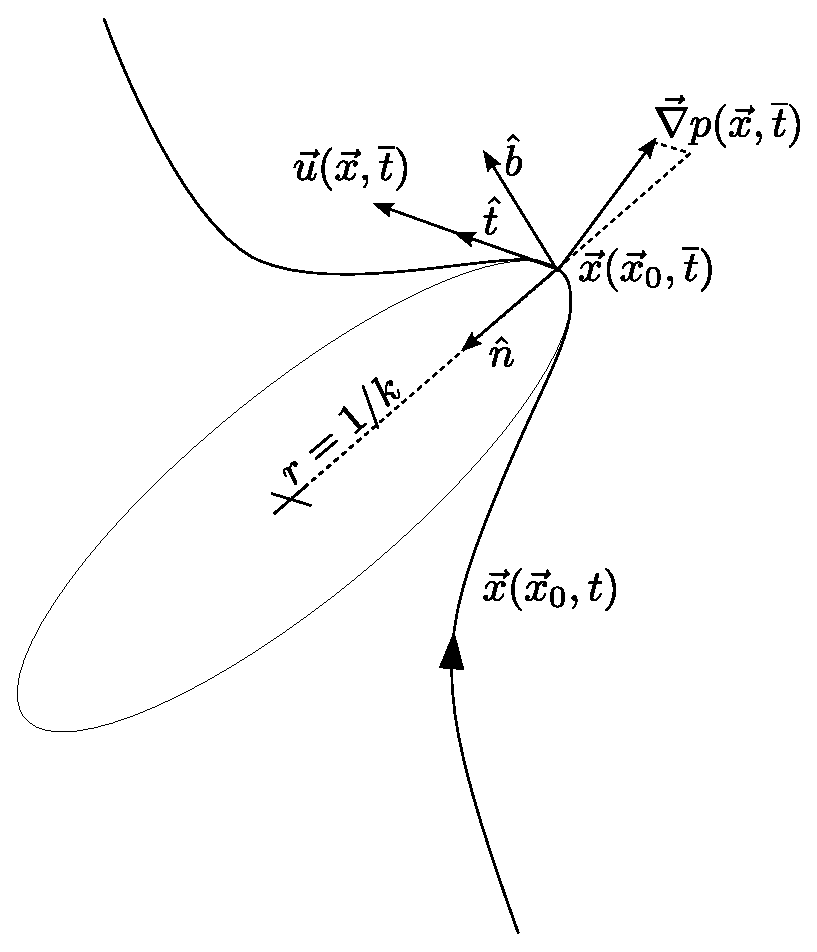
\includegraphics[width=1.0\textwidth]{./fig/frenet.eps}
\end{center}
\end{minipage}
\begin{itemize}
 \item la proiezione del termine forzante lungo la tangente alla traiettoria è la responsabile dell'accelerazione tangenziale della particella materiale;
 \item la proiezione del termine forzante lungo la normale alla traiettoria è la responsabile dell'accelerazione centripeta della particella maetriale e, di conseguenza, della curvatura della traiettoria;
 \item la proiezione della forzante lungo la direzione binormale è nulla.
\end{itemize}

\noindent
In assenza di forze di volume ($\bm{f}=0$) e sforzi viscosi
($\mathbb{T}=\mathbb{S}-p\mathbb{I}=-p\mathbb{I}$):
\begin{equation}
 \begin{cases}
  \rho \frac{dv}{dt} = - \bm{\hat{t}} \cdot \bm{\nabla} p \\
  \rho v^2 k         = - \bm{\hat{n}} \cdot \bm{\nabla} p \\
  0                  = - \bm{\hat{b}} \cdot \bm{\nabla} p \\
 \end{cases}
\end{equation}
%
e quindi:
\begin{itemize}
 \item l'accelerazione tangenziale è proporzionale alla proiezione del gradiente di pressione in direzione tangente alla tratiettoria;
 \item l'accelerazione centripeta, $v^2/r = v^2 k$, è proporzionale alla proiezione del gradiente di pressione in direzione normale alla tratiettoria. Il termine $\rho v^2 k$ è sempre positivo poichè prodotto di quantità positive: la curvatura di una linea è non negativa per come è definita, la densità è positiva, il modulo di un vettore è anch'esso non negativo. Il prodotto scalare tra la normale e il gradiente della pressione (derivata direzionale della pressione in direzione $\bm{\hat{n}}$) deve quindi essere negativo. La pressione quindi diminuisce, andando verso il centro del cerchio osculatore. Sempre dalla seconda equazione è immediato notare che la curvatura della traiettoria è proporzionale alla componente del gradiente di pressione lungo il versore normale;
 \item la proiezione del gradiente di pressione in direzione binormale a una traiettoria è nullo.
\end{itemize}
% Un'analisi della componente normale permette di ricavare, \textbf{sotto le
%  ipotesi fatte}, il legame tra la curvatura delle traiettorie delle
%  particelle fluide e il gradiente del campo di pressione.
% Il termine a sinistra dell'uguale è positivo
% La componente tangente fa aumentare 
%  il modulo della velocità, mentre la componente binormale deve essere nulla.
%Essendo il versore $\bm{\hat{n}}$ diretto verso il centro del cerchio
% osculatore (in parole povere è diretta verso l'interno della curva),
% la curvatura $k$ positiva, segue che la pressione deve diminuire lungo 
% $\bm{\hat{n}}$, cioè aumenta all'allontanarsi dal cerchio del centro
% osculatore (in parole altrettanto povere, ``verso l'esterno'').
%\textit{(Nemmeno a dirlo, la densità $\rho$ è positiva e il quadrato
%  del modulo della velocità $v^2$ è positivo.)}
%\noindent
%Dalla componente lungo $\bm{\hat{n}}$ si nota che il legame tra 
% la componente del gradiente della pressione in quella direzione è
% \textbf{proporzionale} alla curvatura della traiettoria della particella
% fluida.



\subsection{Vorticità}

L'equazione della vorticità in coordinate euleriane è
\begin{equation}
 \frac{\partial \bm{\omega}}{\partial t}
   + (\bm{u}\cdot\bm{\nabla}) \bm{\omega} =
 (\bm{\omega}\cdot\bm{\nabla}) \bm{u} + \nu \bm{\Delta} \bm{\omega}
\end{equation}

Se viene fatta l'ipotesi di viscosità nulla, il termine contenente il 
 laplaciano della vorticità non compare nell'equazione: questo termine
 è il responsabile della diffusione (isotropa per come è scritto) della
 vorticità.
 
L'equazione può essere quindi riscritta come:
 \begin{equation}
  \frac{D\bm{\omega}}{Dt} = (\bm{\omega} \cdot \bm{\nabla}) \bm{u}
 \end{equation}

\noindent 
Scritta in componenti
\begin{equation}
\begin{aligned}
  \frac{D \omega_i}{D t} = \omega_k \frac{\partial u_i}{\partial x_k} \\
\end{aligned}
\end{equation}

\noindent
Il termine di destra può essere riscritto come
\begin{equation}
\begin{aligned}
 \omega_k \frac{\partial u_i}{\partial x_k} & = 
 \omega_k \frac{\partial u_i}{\partial x_{0 l}}
      \frac{\partial x_{0 l}}{\partial x_k} = \qquad \qquad
      \left(u_i = \frac{D x_i}{D t}\right)  \\
 & = \omega_k \frac{D}{Dt} \left( \frac{\partial x_i}{\partial x_{0 l}}
    \right)\frac{\partial x_{0 l}}{\partial x_k} 
\end{aligned}
\end{equation}
Vale la relazione
\begin{equation}
 \frac{\partial x_i}{\partial x_{0 l}}
   \frac{\partial x_{0 l}}{\partial x_k} = \delta_{ik}
\end{equation}
Il termine di sinistra può essere riscritto come
\begin{equation}
 \frac{D \omega_i}{Dt} = \frac{D}{Dt} \left(\delta_{ik} \omega_k \right) =
 \frac{D}{Dt} \left( \frac{\partial x_i}{\partial x_{0 l}}
   \frac{\partial x_{0 l}}{\partial x_k} \omega_k \right)
\end{equation}

Inserendo nell'equazione della vorticità e sfruttando le proprietà
 della derivata del prodotto:
\begin{equation}
\begin{aligned}
 &  \frac{D}{Dt} \left(  \frac{\partial x_i}{\partial x_{0 l}}
   \frac{\partial x_{0 l}}{\partial x_k} \omega_k  \right)  - 
  \omega_k \frac{D}{Dt} \left( \frac{\partial x_i}{\partial x_{0 l}}
    \right)\frac{\partial x_{0 l}}{\partial x_k} = 0 \\
 &  \frac{\partial x_i}{\partial x_{0 l}} 
  \frac{D}{Dt} \left( \frac{\partial x_{0 l}}{\partial x_k} \omega_k
    \right) = 0
\end{aligned}
\end{equation}
Se la trasformazione non è singolare, risulta quindi
\begin{equation}
  \frac{D}{Dt} \left( \frac{\partial x_{0 l}}{\partial x_k} \omega_k
    \right) = 0  \quad \Rightarrow \quad
  \frac{\partial x_{0 l}}{\partial x_k} \omega_k = \omega_{l 0}
\end{equation}
e in conclusione, invertendo il gradiente della trasformazione delle
 coordinate
\begin{equation}\label{eqn:bilanci:vorticitàLagrange}
   \omega_k = \frac{\partial x_k}{\partial x_{0 l}}\omega_{l 0}
   \qquad , \qquad \bm{\omega} = \frac{\partial \bm{x}}{\partial \bm{x}_0}
      \bm{\omega}_0
\end{equation}

Si può quindi notare che la vorticità segue la stessa evoluzione
 di un segmento infinitesimo materiale, per il quale vale:
\begin{equation}
  d\bm{x} = \frac{\partial \bm{x}}{\partial \bm{x}_0}
      d\bm{x}_0
\end{equation}










 

\newpage
% % Relazioni di salto
% % \section{Relazioni di salto}

Si ricavano le condizioni di salto di velocità e sforzo in corrispondenza di superfici di interfaccia.
 Si sottolinea che queste superfici possono essere superfici introdotte dalla modellazione del problema,
 come ad esempio la superficie di separazione tra due fluidi all'interno della quale in generale agisce
 una tensione superficiale o una superficie di discontinuità tangenziale nel caso di fluido non viscoso,
 oppure superfici fittizie.
 
Si parte dai bilanci in forma integrale scritti per un volume in moto arbitrario. I bilanci di massa e quantità di moto
 del volume in moto arbitrario si ottengono dalle regole di derivazione su domini mobili delle funzioni
 $f = \rho$ e $\bm{f} = \rho \bm{u}$,
\begin{equation}
 \frac{d}{dt} \int_{V(t)} f dV 
    = \frac{d}{dt} \int_{v(t)=V(t)} f dv + \oint_{\partial v(t)=\partial V(t)} f(\bm{v}-\bm{w}) \cdot \bm{\hat{n}} ds 
\end{equation}
dove $\bm{u}$ è la velocità del fluido, $\bm{w}$ è la velocità della superficie di discontinuità.

Il billancio integrale viene fatto su un elemento di volume infinitesimo, ``allungato'' nelle direzioni della superficie.
 Quando il volume dell'elemento infinitesimo tende a zero, tende a zero più velocemente dei contributi sulle superfici
 parallele alla superficie di salto.
 
\begin{figure}[h]
\centering
%\captionsetup[subfigure]{labelformat=empty}
\subfloat[][Definizione delle velocità ai due lati dell'elemento infinitesimo e delle dimensioni dello stesso. La velocità 
    della superficie è indicata con $\bm{w}$.]
   {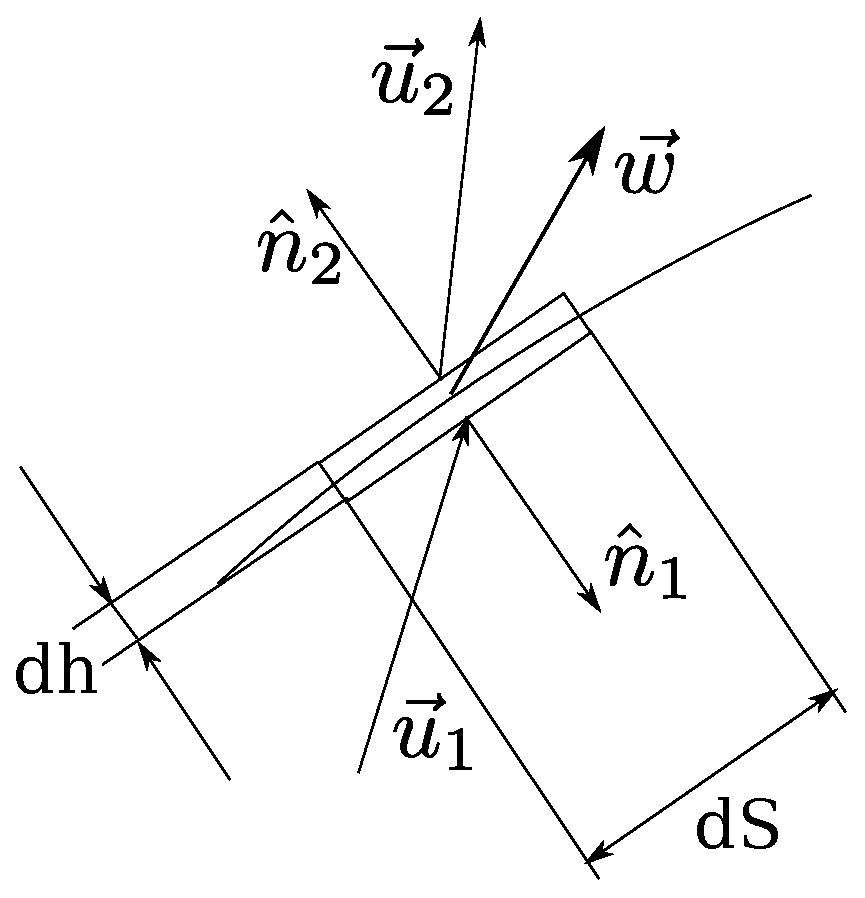
\includegraphics[width=0.30\textwidth]{./fig/elem_velocity.eps}} \qquad \qquad
\subfloat[][Definizione degli sforzi e della tensione superficiale agenti sull'elemento infinitesimo della superficie. ]
   {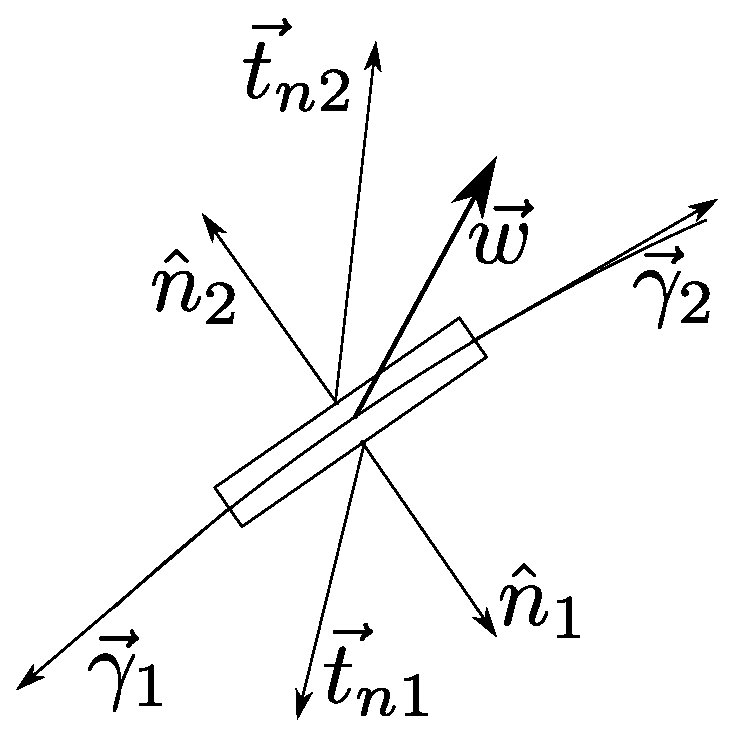
\includegraphics[width=0.30\textwidth]{./fig/elem_stress.eps}}
\end{figure}

L'elemento di volume $dv$ è il parallelepipedo di superfici laterali $dS$, paralleli alla superficie, e basi $dh$ perpendicolari
 alla superficie. Se si ipotizza che le superfici $dh \ll dS$ i contributi nei bilanci dei termini agenti sulle superfici $dh$
 (tranne che nel caso della tensione superficiale, che ha le dimensioni di uno sforzo per una lunghezza) sono trascurabili.


\subsection{Bilancio di massa}
Il bilancio di massa per il volume $dv$  in moto con velocità $\bm{w}$ è
\begin{equation}
 \dfrac{d}{dt}\int_{v} \rho + \oint_{\partial v} \rho (\bm{u} - \bm{w} ) \cdot \bm{\hat{n}} = 0
\end{equation}
Trascurando i contributi di volume e quelli delle superfici $dh$
\begin{equation}
 \rho_1 (\bm{u}_1 - \bm{w} ) \cdot \bm{\hat{n}}_1 dS +  \rho_2 (\bm{u}_2 - \bm{w} ) \cdot \bm{\hat{n}}_2 dS = 0
\end{equation}
dove le normali $\bm{\hat{n}}_1 = \bm{\hat{n}}$ e $\bm{\hat{n}}_2 = -\bm{\hat{n}}$ sono opposte. La quantità tra parentesi è la velocità relativa
 del fluido rispetto alla superficie. Si definisce quindi il flusso di massa $m$ attraverso la superficie.
\begin{equation}
\begin{aligned}
 - m & = \rho_1 (\bm{u}_1 - \bm{w} ) \cdot \bm{\hat{n}} = \rho_2 (\bm{u}_2 - \bm{w} ) \cdot \bm{\hat{n}} \\
   & = \rho_1  \bm{u}_{r1} \cdot \bm{\hat{n}} = \rho_2 \bm{u}_{r2} \cdot \bm{\hat{n}} \\
\end{aligned}
\end{equation}

\noindent
Nel caso di densità uniforme $\rho_1 = \rho_2 = \rho$ si ``conservano'' le componenti normali della velocità relativa e della
 velocità.
\begin{equation}
\begin{aligned}
  \bm{u}_{r1} \cdot \bm{\hat{n}} & = \bm{u}_{r2} \cdot \bm{\hat{n}} \\
  \bm{u}_{1}  \cdot \bm{\hat{n}} & = \bm{u}_{2}  \cdot \bm{\hat{n}} \\
\end{aligned}
\end{equation}


\subsection{Bilancio di quantità di moto}
Il bilancio della quantità di moto per l'elemento $dv$ è
\begin{equation}
 \dfrac{d}{dt}\int_{v} \rho\bm{u} + \oint_{\partial v} \rho \bm{u}(\bm{u} - \bm{w} ) \cdot \bm{\hat{n}} = \oint_{\partial v} \bm{t_n} + \int_{v} \rho \bm{g} + \int_{l} \bm{\gamma}
\end{equation}
avendo incluso anche eventuali termini di tensione superficiale, svolto 
 sulla curva che separa tre sostanze (come ad esempio il ``perimetro''
 del menisco visto nell'esercizio sul capillare: in quel caso la curva
 $l$ separa il liquido, dall'aria, dalle pareti solide del capillare).
Trascurando i termini di volume, il bilancio per l'elemento infinitesimo (per semplicità pensato in 2 dimensioni) è
\begin{equation}
 \rho_1 \bm{u}_1 (\bm{u}_1 - \bm{w})\cdot \bm{\hat{n}}_1 ds + \rho_2 \bm{u}_2 (\bm{u}_2 -\bm{w}) \cdot \bm{\hat{n}}_2 ds =
    \bm{t_{n1}} ds + \bm{\gamma}_1  + \bm{t_{n2}} ds + \bm{\gamma}_2 
\end{equation}
con $\bm{\gamma}_1 = \gamma \bm{\hat{t}_1}$, $\bm{\gamma}_2 = (\gamma + \gamma_{/s} ds) \bm{\hat{t}_2}$. I versori 
 tangenti $\bm{\hat{t}}_1$, $\bm{\hat{t}}_2$ agli estremi dell'elementino di superficie non sono allineati a causa della curvatura della superficie (si
rimanda alla ``dimostrazione'' della legge di Young-Laplace). Si tiene conto di una possibile
 variazione della tensione superficiale. Questa di solito può essere
 dovuta a differenze di temperatura o composizioni chimiche (perchè si
usa il sapone per lavarsi le mani?): si rimanda al 
 simpatico (?) video delle barchette sul fondo del documento della dimostrazione
 della legge di Young-Laplace, nel quale viene usata una ``propulsione a effetto Marangoni'' per barchette di carta. Il contributo della tensione superficiale si può scrivere come
\begin{equation}
 \bm{\gamma}_2 + \bm{\gamma}_1 = (2 \gamma H \bm{\hat{n}} + \bm{\nabla}_2 \gamma )ds
\end{equation}
dove
\begin{itemize}
 \item H è la curvatura media $H = \frac{1}{2}\left(\frac{1}{R_1} + \frac{1}{R_2}\right)$ nel caso tridimensionale, che nel caso bidimensionale
 coincide con $ \frac{1}{2 R}$ (uno dei due raggi di curvatura diventa infinito).
 \item $\bm{\hat{n}}$ è il vettore normale che punta verso i centri di
 curvatura.
 \item $\bm{\nabla}_2$ è il gradiente ristretto alla superficie, tangente ad essa.
\end{itemize}

\noindent
Ricordando la definizione di $m$ e inserendola nel bilancio
\begin{equation}
 m ( \bm{u}_1 - \bm{u}_2 ) =
    \bm{t_{n1}} + \bm{t_{n2}} + 2 \gamma H \bm{\hat{n}} + \bm{\nabla}_2 \gamma
\end{equation}

\noindent
Si analizzano ora alcuni casi particolari:
\begin{itemize}
\item Statica con tensione superficiale. La velocità è nulla ovunque, i vettori di sforzo hanno solo il contributo della pressione
 $\bm{t_n} = -p \bm{\hat{n}}$. Secondo queste ipotesi, non si possono avere contributi tangenziali nemmeno a causa della tensione 
 superficiale e quindi $\gamma$ deve essere uniforme sulla superficie. Nel caso bidimensionale si ricorda che la normale $\bm{\hat{n}}$
 punta verso il centro del cerchio osculatore e coincide quindi con la normale $\bm{\hat{n}}_1$ dell'immagine e il raggio di curvatura $R$ è positivo.
 Il bilancio della quantità di moto si riduce all'equilibrio statico della superficie
 \begin{equation}
   p_1 - p_2 = \frac{\gamma}{R}
 \end{equation}
 Si osserva quindi che la pressione ``interna'' $p_1$ deve essere maggiore di $p_2$.
\item Fluido inviscido, superficie senza tensione superficiale. Il bilancio si riduce a 
\begin{equation}
  m ( \bm{u}_1 - \bm{u}_2 ) = - (p_1 - p_2) \bm{\hat{n}}
\end{equation}
\item Fluido inviscido, superficie senza tensione superficiale, densità uniforme. Si è visto come la 
  velocità (e le velocità relative) normali alla superficie devono essere uguali da entrambe le parti
  della superficie. %Se la superficie è una superficie materiale, la velocità della superficie coincide
%  con quella del fluido e quindi la velocità relativa è nulla ed $m = 0$.
%  Risulta quindi che non ci può essere salto di pressione attraverso una tale superficie (questo è quello che significa
%  l'ipotesi espressa in termini pittoreschi di ``scia scarica'' nell'aerodinamica a potenziale).
%  \begin{equation}
%    p_1 = p_2
%  \end{equation}
  Se si ipotizza che la superifice non sia attraversata da flusso di massa (si impone che la componente normale della velocità relativa sia nulla,
  non la velocità relativa nel suo complesso). In questo caso non è possibile trovare una relazione 
  di salto per la velocità tangenziale (o almeno questo non è possibile se non si aggiungono altre ipotesi o altre equazioni \dots vedremo 
  un caso semplificato applicando il teorema di Bernoulli a un problema aerodinamico bidimensionale stazionario \dots):
  poichè $m=0$ la superficie è ``scarica'' (capiterà nei prossimi corsi di sentir parlare o aver direttamente a che fare con ``
  l'ipotesi di scia scarica'': questa non dovrà quindi essere una novità o una sorpresa in futuro)
  \begin{equation}
    p_1 = p_2
  \end{equation}
  ma non si riesce a ricavare nessuna informazione dalla componente tangenziale
  dell'equazione poichè è un'identità $0=0$ a prescindere dal valore di $( \bm{u}_1 - \bm{u}_2 )\cdot \bm{\hat{t}}$. Attraverso tale superficie
  (di spessore nullo) ci può essere un salto finito di velocità tangenziale: in questo caso la superficie è una superficie di vorticità infinita
\end{itemize}

\noindent
L'ultimo caso particolare verrà utilizzato in qualche esercizio in cui un dominio occupato da un fluido può essere suddiviso in un sottodominio 
 nel quale è valido il teorema di Bernoulli (in qualche forma \dots) e in un sottodominio dove sono valide le relazioni della statica: le condizioni
 di salto serviranno a far comunicare tra di loro i due sottodomini (e a risolvere correttamente l'esercizio).

\subsection{Bilancio di energia}
Non verrà detto nulla sulle relazioni di salto delle altre quantità \dots

 
% \newpage
% Introduzione agli esercizi
\section{Introduzione agli esercizi}

I bilanci integrali consentono di valutare le azioni integrali (forze, momenti, potenza) scambiati tra un fluido e un corpo a contatto con esso, senza conoscere nel dettaglio il campo di moto del fluido di interesse, ma valutando il flusso netto delle quantità meccaniche di interesse (massa, quantità di moto, momento della quantità di moto, energia, entalpia e calore) attraverso la superficie di contorno del volume fluido di interesse.
%
Il contorno del dominio fluido $v(t)$ viene suddiviso nella parte a contatto con il corpo di interesse $s_{f,s}(t)$ e nella parte rimanente $s_{f,free}(t) = \partial v(t) \backslash s_{f,s}(t)$.

\paragraph{Bilancio della quantità di moto e risultante delle forze.}
La risultante delle forze agenti sul corpo\footnote{La risultante delle forze delle azioni scambiate con il fluido. A questa andranno sommate le forze di volume, come ad esempio il peso del corpo stesso.} sarà uguale all'integrale del vettore sforzo agente sulla superficie $s_{s,f}(t)$,
\begin{equation}
 \bm{R}^s = \oint_{s_{s,f}(t)} \bm{t}_{n,s} \ ,
\end{equation}
avendo indicato con $s_{s,f}(t)$ la superficie del solido con normale uscente dalla superficie solida ed entrante nel solido e con $\bm{t}_{n,s}$ il vettore sforzo agente sul solido, uguale e contrario allo sforzo agente sul fluido nello stesso punto, $\bm{t}_{n,s} = - \bm{t}_n$, per il principio di azione e reazione (terzo principio della dinamica). Non è stato aggiunto il pedice $f$ al vettore sforzo agente sul fluido, poiché siamo in un corso di fluidodinamica e il soggetto è il fluido, quando è sottointeso.
Si può riconoscere la risultante $\bm{R}^s$ all'interno del bilancio integrale della quantità di moto per il volume fluido $v(t)$,
\begin{equation}
\begin{aligned}
 \dfrac{d}{dt} \displaystyle\int_{v(t)} \rho \bm{u} + \oint_{\partial v(t)} \rho \bm{u} (\bm{u}-\bm{v}) \cdot \bm{\hat{n}}= \int_{v(t)} \bm{f} + \oint_{\partial v(t)} \bm{t_n} \ .
\end{aligned}
\end{equation}
Si analizzano i termini di superficie, considerando separatamente i contributi delle superfici $s_{f,s}$ e $s_{f,free}$. Se il solido ha una superficie impermeabile al fluido e non c'è flusso di massa, la velocità del fluido e del solido sono uguali, $\bm{u} = \bm{v}$, sulla superficie $s_{f,s}$. Di conseguenza rimane solo il contributo del flusso della quantità di moto attraverso la superficie $s_{f,free}$, mentre il termine di flusso attraverso $s_{f,s}$ è nullo.
L'integrale sul contorno $\partial v(t)$ del vettore sforzo può essere suddiviso nella somma dell'integrale svolto sulla superficie a contatto con il solido e sulla superficie libera,
\begin{equation}
\begin{aligned}
 \oint_{\partial v(t)} \bm{t_n} & = 
 \oint_{s_{f,s}(t)} \bm{t_n} + \oint_{s_{f,free}(t)} \bm{t_n} = \\
 & = - \oint_{s_{s,f}(t)} \bm{t}_{n,s} + \oint_{s_{f,free}(t)} \bm{t_n} =
 -\bm{R}^s + \oint_{s_{f,free}(t)} \bm{t_n} \ .
\end{aligned}
\end{equation}
Spesso sulla superficie libera $s_{f,free}(t)$ possono essere trascurati gli sforzi viscosi: in questo caso, il vettore sforzo si riduce al solo effetto della pressione $\bm{t_n} = -p \bm{\hat{n}}$.

Ritornando al bilancio della quantità di moto, si può scrivere
\begin{equation}
 \bm{R}^s = - \int_{s_{f,free}} \rho \bm{u} (\bm{u}-\bm{v}) \cdot \bm{\hat{n}}
 - \int_{s_{f,free}(t)} \bm{t_n}
 - \int_{v(t)} \bm{f} - \dfrac{d}{dt} \int_{v(t)} \rho \bm{u}
\end{equation}
Nel caso in cui il problema sia stazionario e che le forze di volume nel fluido siano trascurabili, gli ultimi due termini is annullano. Se poi si possono trascurare gli sforzi viscosi su $s_{f,free}$, la superficie $s_{s,free}$ è una superficie chiusa (si pensi alla superficie ``all'infinito'' attorno a un corpo, come esempio) e la pressione è costante su questa superficie chiusa, l'integrale degli sforzi su $s_{f,free}$ è anch'esso nullo, poiché
\begin{equation}
 \oint_{s_{f,free}(t)} \bm{t_n} = - \oint_{s_{f,free}(t)} p \bm{\hat{n}} = - p \oint_{s_{f,free}(t)} \bm{\hat{n}} \equiv 0 \ ,
\end{equation}
e la risultante delle forze agenti sul solido si riduce a
\begin{equation}
 \bm{R}^s = - \int_{s_{f,free}} \rho \bm{u} (\bm{u}-\bm{v}) \cdot \bm{\hat{n}} \ .
\end{equation}

\paragraph{Bilancio del momento della quantità di moto e risultante dei momenti.}
Riproponendo un ragionamento analogo, dal bilancio del momento della quantità di moto si può ricavare la risultante dei momenti agenti su un corpo,
\begin{equation}
 \bm{M} = \oint_{s_{s,f}} \bm{r} \times \bm{t}_{n,s} \ .
\end{equation}
 Nel caso semplificato in cui il problema sia stazionario, le forze di volume sono trascurabili, gli sforzi viscosi sono trascurabili sulla superficie $s_{f,free}(t)$ chiusa, sulla quale agisce una pressione costante, la risultante dei momenti agenti sul solido si riduce a
\begin{equation}
 \bm{M}^s = - \int_{s_{f,free}} \rho \bm{r} \times \bm{u} (\bm{u}-\bm{v}) \cdot \bm{\hat{n}} \ ,
\end{equation}
dove $\bm{r}$ è il raggio vettore tra i punti sulla superficie $s_{f,free}(t)$ e il polo rispetto al quale si calcolano i momenti.

\paragraph{Bilancio dell'energia totale.}
Tramite il bilancio dell'energia totale si può ricavare la potenza fornita (o assorbita) da un corpo al fluido, e/o il calore scambiato con esso. Gli esercizi che utilizzeranno il bilancio di energia totale ricorderanno alcuni esercizi di Fisica Tecnica. Lo scopo di questi esercizi è quello di proporre un punto di vista più maturo a tali problemi, partendo ai bilanci integrali nella loro forma più generale e opportunamente semplificati considerando grandezze uniformi sulle sezioni (o equivalenti grandezze medie) e ipotesi sullo scambio di calore tra il fluido e l'esterno. Verranno analizzati sistemi aperti e chiusi, nella speranza di fornire un approccio di validità generale a problemi già trattati durante il corso di Fisica Tecnica, senza alcuna pretesa di coprire tutti gli argomenti e i dettagli trattati in quel corso, ma piuttosto consentire una visione del problema generale che coinvolga scambi di massa, lavoro e calore del sistema con l'esterno, facilmente specializzabile a casi particolari, che riduca al minimo lo sforzo mnemonico richiesto da molti casi particolari, apparentemente scorrelati l'uno dall'altro, a vantaggio di una maggiore ``sensibilità'' sul fenomeno fisico.

Sfruttando la suddivisione della superficie del volume fluido $\partial v = s_{f,free} \cup s_{f,s}$, si può riscrivere il bilancio dell'energia totale,
\begin{equation}
 \dfrac{d}{dt} \displaystyle\int_{v(t)} \rho e^t + \oint_{\partial v(t)} \rho e^t (\bm{u}-\bm{v}) \cdot \bm{\hat{n}}= \int_{v(t)} \bm{f} \cdot \bm{u} + \oint_{\partial v(t)} \bm{t_n} \cdot \bm{u} - \oint_{\partial v(t)} \bm{q} \cdot \bm{\hat{n}} + \int_{v(t)} \rho r \ .
\end{equation}
riconoscendo la potenza
\begin{equation}
 W = \oint_{s_{f,s}} \bm{t_n} \cdot \bm{u} \ ,
\end{equation}
 fornita da un corpo solido al fluido,
\begin{equation}
\begin{aligned}
 \dfrac{d}{dt} \displaystyle\int_{v(t)} \rho e^t & + \oint_{\partial v(t)} \rho e^t (\bm{u}-\bm{v}) \cdot \bm{\hat{n}} = \\
  & = \int_{v(t)} \bm{f} \cdot \bm{u} + \oint_{s_{f,free}(t)} \bm{t_n} \cdot \bm{u} + W - \oint_{\partial v(t)} \bm{q} \cdot \bm{\hat{n}} + \int_{v(t)} \rho r \ .
\end{aligned}
\end{equation}
Se non c'è flusso di massa attraverso la superficie solida, $\bm{u} = \bm{v}$ su $s_{f,s}$. Se la superficie libera $s_{f,free}$ del volume di controllo è fissa, $\bm{v}= \bm{0}$ su $s_{f,free}$. Separando il contributo degli sforzi di pressione da quelli viscosi, $\bm{t_n} = -p\bm{\hat{n}} + \bm{s_n}$ sulla superficie $s_{s,free}$, il bilancio dell'energia totale diventa,
\begin{equation}
\begin{aligned}
 \dfrac{d}{dt} \displaystyle\int_{v(t)} \rho e^t & + \oint_{s_{f,free}(t)} \rho h^t \bm{u} \cdot \bm{\hat{n}} = \\
  & = \int_{v(t)} \bm{f} \cdot \bm{u} + \oint_{s_{f,free}(t)} \bm{s_n} \cdot \bm{u} + W - \oint_{\partial v(t)} \bm{q} \cdot \bm{\hat{n}} + \int_{v(t)} \rho r \ ,
\end{aligned}
\end{equation}
avendo introdotto l'entalpia totale $h^t = e^t + \frac{p}{\rho} = e + \frac{p}{\rho} + \frac{|\bm{u}|^2}{2}$.
%
Se si trascurano la potenza degli sforzi viscosi su $s_{s,free}$ e la potenza delle forze di volume $\bm{f}$, il bilancio dell'energia totale del fluido contenuto nel volume $v(t)$ diventa
\begin{equation}
 \dfrac{d}{dt} \displaystyle\int_{v(t)} \rho e^t + \oint_{s_{f,free}(t)} \rho h^t \bm{u} \cdot \bm{\hat{n}}
 \, = \,
  W - \oint_{\partial v(t)} \bm{q} \cdot \bm{\hat{n}} + \int_{v(t)} \rho r \ .
\end{equation}

\paragraph{Sistemi aperti}
Per un sistema aperto in cui sono soddisfatte le ipotesi già elencate, si può scrivere
\begin{equation}
 \dfrac{d}{dt} \displaystyle\int_{v(t)} \rho e^t = - \oint_{s_{f,free}(t)} \rho h^t \bm{u} \cdot \bm{\hat{n}}
  + W - \oint_{\partial v(t)} \bm{q} \cdot \bm{\hat{n}} + \int_{v(t)} \rho r \ ,
\end{equation}
e sinteticamente
\begin{equation}
  \dfrac{d E^t}{d t} = \Phi_{h^t} + W + \dot{Q} \ ,
\end{equation}
avendo definito l'energia totale interna $E^t$ al volume $v(t)$ studiato, il flusso netto di entalpia totale $\Phi_{h^t}$ attraverso la superficie $s_{s,free}$, e il flusso di calore $\dot{Q}$ fornito al fluido contenuto all'interno di $v(t)$,
\begin{equation}
\begin{aligned}
  E & = \int_{v(t)} \rho e \\
  \Phi_{h^t} & = \int_{s_{f,free}} \rho h^t \bm{u} \cdot \bm{\hat{n}}
               = \int_{s_{f,free}} \rho \left( e + \dfrac{p}{\rho} + \dfrac{|\bm{u}|^2}{2} \right) \bm{u} \cdot \bm{\hat{n}} \\
 \dot{Q} & = - \oint_{\partial v(t)} \bm{q} \cdot \bm{\hat{n}} + \int_{v(t)} \rho r \ . 
\end{aligned}
\end{equation}

\paragraph{Sistemi chiusi}
Per un sistema chiuso (nessuno scambio di massa con l'esterno) in cui i termini cinetici sono trascurabili, $e^t = e$, il bilancio di energia diventa sintenticamente,
\begin{equation}
%\dfrac{d}{dt} \displaystyle\int_{v(t)} \rho e 
%\, = \,
% W - \oint_{\partial v(t)} \bm{q} \cdot \bm{\hat{n}} + \int_{v(t)} \rho r
%\qquad \rightarrow \qquad
 \dfrac{d E}{dt} = W + \dot{Q} \ ,
\end{equation}
avendo definito $E = \displaystyle\int_{v(t)} \rho e$, come l'energia interna del fluido contenuto nel volume $v(t)$.
Questa formula corrisponde al primo principio della Termodinamica, formulato in termini di potenza e non di energia, in cui è stata utilizzata la convenzione di potenza delle forze positiva e flusso di calore positivo se fornito al fluido.\footnote{In Termodinamica, che studia sistemi in equilibrio, il primo principio è formulato in termini di energia come,
\begin{equation}
 \Delta E = Q - L \ ,
\end{equation}
in cui la variazione di energia $\Delta E$ tra due stati termodinamici del sistema corrisponde alla differenza del calore $Q$ fornito al sistema e al lavoro $L$ svolto \textbf{dal} sistema.
}

% Affrontare i problemi partendo dalla forma generale dei bilanci dovrebbe consentire lo studio di sistemi con scambio di massa, lavoro e flussi di calore

% 
% I bilanci integrali di massa e quantità di moto consentono di calcolare le azioni integrali (forze e momenti) scambiati tra un fluido e un corpo. Per studiare l'interazione \textit{integrale} di un fluido con un corpo fermo (in un sistema di riferimento inerziale) è conveniente usare una descrizione euleriana del problema.
% %, per la quale i bilanci delle quantità meccaniche in un volume di controllo $V_c$ fisso sono,
% %\begin{equation}
% % \begin{cases}
% %   \dfrac{d}{d t} \displaystyle\int_{V_c} \rho + \oint_{S_c} \rho \bm{u} \cdot \bm{\hat{n}} = 0 \\
% %   \dfrac{d}{d t} \displaystyle\int_{V_c} \rho  \bm{u}+ \oint_{S_c} \rho \bm{u} \bm{u} \cdot \bm{\hat{n}} = \int_{V_c} \bm{f} + \oint_{S_c} \bm{t_n} \\
% %   \dfrac{d}{d t} \displaystyle\int_{V_c} \rho \bm{r} \times \bm{u}+ \oint_{S_c} \rho \bm{r} \times \bm{u} \bm{u} \cdot \bm{\hat{n}} = \int_{V_c} \bm{r} \times \bm{f} + \oint_{S_c} \bm{r} \times \bm{t_n} \\
% %   \dfrac{d}{d t} \displaystyle\int_{V_c} \rho  e^t+ \oint_{S_c} \rho e^t \bm{u} \cdot \bm{\hat{n}} = \int_{V_c} \bm{f} \cdot \bm{u} + \oint_{S_c} \bm{t_n} \cdot \bm{u} - \oint_{S_c} \bm{q} \cdot \bm{\hat{n}} \ .
% % \end{cases}
% %\end{equation}
% I bilancio integrale può essere utilizzato per calcolare delle grandezze fisiche integrali incognite:
% \begin{itemize}
%  \item flussi di massa (portate massiche) dal bilancio di massa;
%  \item risultanti di forze dal bilancio di quantità di moto;
%  \item risultanti di momenti dal bilancio del momento della quantità di moto;
%  \item potenze dal bilancio dell'energia.
% \end{itemize}
% Per esempio, nel caso stazionario in cui la pressione del fluido è uniforme sulla superficie esterna $S_f$ del volume di controllo e le forze di volume sono trascurabili, la risultante delle forze e dei momenti agenti su un corpo solido valgono
% \begin{equation}
% \begin{cases}
%  \bm{R} = -\displaystyle\oint_{S_f} \rho \bm{u} \bm{u} \cdot \bm{\hat{n}} \\
%  \bm{M} = -\displaystyle\oint_{S_f} \rho \bm{r} \times \bm{u} \bm{u} \cdot \bm{\hat{n}}  \ ,
% \end{cases}
% \end{equation}
% avendo indicato con $\bm{r}$ il raggio tra il punto nel fluido e il polo, rispetto al quale è calcolato il momento.
% Per casi più generali, in cui la pressione non è uniforme, si rimanda allo svolgimento degli esercizi.
% 


\newpage \clearpage

% Esercizi
%> === Bilancio di massa ========================================
\noindent
\begin{tabular}{cc}
\begin{minipage}{0.65\textwidth}
\begin{exerciseS}[Bilancio di massa: teoria delle reti]
Si consideri  una rete idraulica come quella rappresentata in figura.
All'interno dei tubi scorre acqua. Sia nota le velocit\`a media
dell'acqua all'interno di alcuni dei rami della rete: 
$U_1 = 1\, m/s$, $U_2 = 1.5\, m/s$, $U_3 = 0.5\, m/s$,
$U_7 = 2\, m/s$ e $U_8 = 0.3\, m/s$. 
Il verso della velocit\`a è indicato dalle frecce 
sul disegno.
Determinare la portata volumetrica, la portata in massa e la velocit\`a
media all'interno di ciascun ramo della rete 
sapendo che l'acqua ha una densit\`a pari a $\overline{\rho} = 999\ kg/m^3$,
e che il diametro dei tubi \`e rispettivamente $D_1=0.4\ m$, 
$D_2=0.2\ m$, $D_3=0.2\ m$, $D_4=0.3\ m$, $D_5=0.5\ m$,
$D_6=0.25\ m$, $D_7=0.3\ m$, $D_8=0.6\ m$.

($Q_1 = 0.13\ m^3/s$, $Q_2 = 0.05\ m^3/s$, $Q_3 = 0.02\  m^3/s$, 
 $Q_4 = 0.13\ m^3/s$, $Q_5 = 0.06\ m^3/s$, $Q_6 = 0.13\  m^3/s$, 
 $Q_7 = 0.14\ m^3/s$, $Q_8 = 0.08\ m^3/s$,
 $U_1 = 1\ m^3/s$, $U_2 = 1.5\  m^3/s$, $U_3 = 0.5\  m^3/s$, 
 $U_4 = 1.87\ m^3/s$, $U_5 = 0.29\  m^3/s$, $U_6 = 2.69\  m^3/s$, 
 $U_7 = 2\  m^3/s$, $U_8 = 0.3\ m^3/s$,
 $\overline{Q}_1 = 125.5\  kg/s$, $\overline{Q}_2 = 47.08\  kg/s$,
 $\overline{Q}_3 = 15.69\  kg/s$, 
 $\overline{Q}_4 = 131.8\  kg/s$, $\overline{Q}_5 = 54.49\  kg/s$,
 $\overline{Q}_6 = 131.8\  kg/s$, 
 $\overline{Q}_7 = 141.2\  kg/s$, $\overline{Q}_8 = 84.74\  kg/s$)
\end{exerciseS}
\end{minipage}
&
\begin{minipage}{0.35\textwidth}
   \begin{center}
   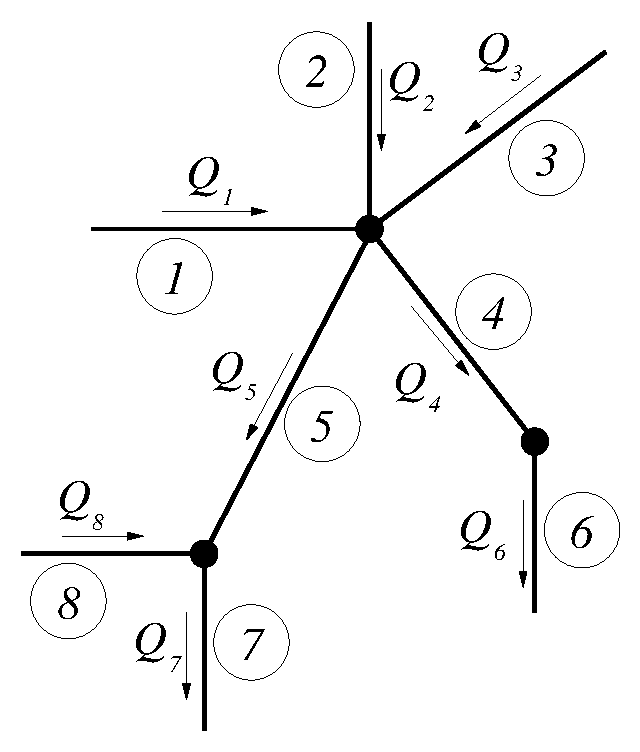
\includegraphics[width=0.90\textwidth]{./fig/rete.eps}
   \end{center}
\end{minipage}
\end{tabular}

\sol

\partone
Bilancio integrale della massa. Teoria delle reti: bilancio ai nodi.

\parttwo
Se il regime di moto è stazionario, la portata massica è costante e indipendente dalla sezione considerata all'interno di ogni singolo tubo. Il bilancio di massa nell'$i$-esimo tubo è,
\begin{equation}
 \underbrace{\dfrac{d}{dt} \int_{V_i} \bm{\rho}}_{=0} = \oint_{S_i} \rho \bm{u} \cdot \bm{\hat{n}} = \oint_{S_{i,{\alpha}}}\rho \bm{u} \cdot \bm{\hat{n}} + \oint_{S_{i,\beta}} \rho \bm{u} \cdot \bm{\hat{n}} = \tilde{Q}_{i,\alpha} + \tilde{Q}_{i,\beta} \quad \rightarrow \quad \tilde{Q}_{i,\alpha} = -  \tilde{Q}_{i,\beta} \ , 
\end{equation}
avendo indicato $S_{i,{\alpha}}$ e $S_{i,{\beta}}$ le due sezioni in ``ingresso'' e ``uscita'' del tubo $V_i$, con $\bm{\hat{n}}$, $\tilde{Q}_{\alpha}$ e $\tilde{Q}_{\beta}$ la normale uscente e i flussi di massa uscenti dal volume $V_i$. Se si calcola il flusso di massa $\overline{Q}_i$ attraverso le sezioni del tubo con normale identificata dal ``verso di percorrenza'' del tubo, uno dei due termini cambia segno e si dimostra che la portata è costante sulle sezioni del singolo tubo, 
\begin{equation}
 \overline{Q}_{i,\alpha} = \overline{Q}_{i,\beta} =: \overline{Q}_{i} \ .
\end{equation}
%
Utilizzando il verso delle frecce indicato in figura per stabilire il segno dei flussi di massa, il bilancio di massa ai nodi porta al sistema lineare,
\begin{equation}
 \begin{cases}
   \overline{Q}_1 + \overline{Q}_2 + \overline{Q}_3 - \overline{Q}_4 - \overline{Q}_5 = 0 & \text{(bil. al nodo in alto)} \\
   \overline{Q}_5 + \overline{Q}_8 - \overline{Q}_7 = 0 & \text{(bil. al nodo a sinistra)} \\
   \overline{Q}_4 - \overline{Q}_6 = 0 & \text{(bil. al nodo a destra)} \ , \\
 \end{cases}
\end{equation}
nel quale le incognite sono i flussi $\overline{Q}_4$, $\overline{Q}_5$, $\overline{Q}_6$, una volta calcolati gli altri flussi con i dati forniti dal testo del problema,
$\overline{Q}_k = \rho \frac{\pi}{4}D_k^2 U_k$, $k=1,2,3,7,8$.
%
Successivamente si calcolano le portate volumetriche $Q_k$ incognite, dividendo le portate massiche $\overline{Q}_k$ per la densità $rho$,
\begin{equation}
 Q_k = \dfrac{\overline{Q}_k}{\rho} \quad , \quad k = 1:8 \ .
\end{equation}

%\begin{equation}
% \begin{cases}
%   Q_1 + Q_2 + Q_3 - Q_4 - Q_5 = 0 & \text{(bil. al nodo in alto)} \\
%   Q_5 + Q_8 - Q_7 = 0 & \text{(bil. al nodo a sinistra)} \\
%   Q_4 - Q_6 = 0 & \text{(bil. al nodo a destra)} \\
% \end{cases}
%\end{equation}

%\item
%Si ricavano le velocità ancora incognite:
%\begin{equation}
%  U_i = \frac{Q_i}{S_i}, \qquad i = 4,5,6
%\end{equation}

%\item
%Infine si calcolano le portate in massa semplicemente moltiplicando 
%quelle volumetriche per la densità $\bar{\rho}$:
%\begin{equation}
%  \bar{Q_i} = \bar{\rho} Q_i, \qquad i = 1:8
%\end{equation}

%\end{itemize}
 % teoria delle reti
\newpage
\noindent
\begin{tabular}{cc}
\begin{minipage}{0.95\textwidth}
\begin{exerciseS}[Bilancio di massa: riempimento bombola]
Si sta riempiendo una bombola per immersioni subacquee.
Sapendo che la pompa aspira aria a pressione ambiente di 
$1.01\times10^5\ Pa$ e alla temperatura di $293\ K$
in un condotto di sezione $1\ cm^2$ in cui la velocit\`a media \`e di 
$0.5\ m/s$ e che non ci sono perdite nel sistema di pompaggio,
determinare la rapidit\`a di variazione della massa d'aria e della sua 
densit\`a all'interno della bombola, sapendo che il volume della bombola
\`e pari a $0.02 \  m^3$.

($\frac{dM}{dt} = 6.01 \times 10^{-5}\ kg/s, \frac{d \rho}{d t} = 3.00 \times 10^{-3}\ kg/(m^3 s)$).
\end{exerciseS}
\end{minipage}
\end{tabular}

\sol

\partone Bilancio integrale della massa. Legge dei gas perfetti.

\parttwo
Sono date la pressione $p$ e la temperatura $T$ all'uscita della pompa.
\'E nota l'area $S$ della sezione e la velocità media $U$ su quella
 sezione. 
% Se si suppone che il gas sia un gas ideale perfetto, si può ricavare la densità come $\rho = \frac{p}{R T}$. Si può quindi calcolare il flusso di massa $\dot{m}$.
%
Si trova la variazione di massa all'interno della bombola grazie al bilancio integrale di massa nel volume della bombola $V$ (volume di controllo, fisso),
\begin{equation}
 \dfrac{d M}{d t} = \dfrac{d}{d t} \int_V \rho = -\oint_S \rho \bm{u} \cdot \bm{u} =
 \rho_{in} S_{in} U \ ,
\end{equation}
dove si è indicato con $M$ la massa totale, $S_{in}$ l'area della sezione del tubo utilizzato per riempire la bombola e $\rho_{in}$, la densità sulla sezione di ingresso, dove sono note la pressione $P_{in}$ e la temperatura $T_{in}$. Ipotizzando che valga la legge di stato dei gas perfetti, la densità sulla sezione di ingresso vale
\begin{equation}
 \rho_{in} = \dfrac{P_{in}}{R T_{in}} \ ,
\end{equation}
dove $R=287 J/(kg\ K)$ è la costante dei gas per l'aria. La derivata nel tempo della massa d'aria nella bombola vale quindi
\begin{equation}
  \frac{d M}{d t} = 6.0 \cdot 10^{-5} \dfrac{kg}{s} \ .
\end{equation}
%
Supponendo che la densità dell'aria si uniforme all'interno della bombola, si può calcolare la sua derivata nel tempo, 
\begin{equation}
 \dfrac{d \rho}{d t} = \dfrac{1}{V} \dfrac{d}{dt} \int_V \rho = 2.0 \cdot 10^{-3} \dfrac{kg}{m^3 s} \ .
\end{equation}


%\begin{equation}
%  \dot{m} = \rho S U
%\end{equation}

%La derivata della massa contenuta nella bombola è uguale al flusso entrante nella bombola, uguale al flusso uscente dalla pompa (nell'ipotesi che non ci siano perdite).

%\begin{equation}
% \frac{d M}{d t} = \rho S U  \quad \Rightarrow \quad
%  \frac{d M}{d t} = 6.0 \cdot 10^{-5} kg/ s
%\end{equation}

%Per calcolare la derivata della densità all'interno della bombola, si 
%osserva che il volume della bombola non cambia. La derivata della 
%massa è $\frac{d M}{d t} = \frac{d (\rho V)}{d t} = V \frac{d \rho}
%{d t}$.

%\begin{equation}
% \frac{d \rho}{d t} = \frac{\rho U S}{V} \quad \Rightarrow \quad
%  \frac{d \rho}{d t} = 2.0 \cdot 10^{-3} kg/(m^3 s)
%\end{equation}
 % riempimento bombola

%> === Bilancio di quantità di moto e risultante sui corpi ======
\newpage

\noindent
\begin{tabular}{cc}
\begin{minipage}{0.60\textwidth}
\begin{exerciseS}[Effetto Coanda sul cilindro]
Un getto d'acqua ($\rho=999\ kg/m^3$) stazionario, piano e orizzontale 
viene indirizzato su un cilindro, lambendone la superficie e
venendo deviato di un angolo $\alpha =15^\circ$.
Determinare la forza agente su una porzione del cilindro di lunghezza 
pari a $H = 2\ m$, dovuta sia al getto d'acqua,
sia all'aria circostante, sapendo che:
\begin{itemize}
  \item il fluido che circonda il getto e il cilindro \`e aria in quiete a
  pressione atmosferica di $101325\ Pa$;
  \item la larghezza del getto \`e $h=2\ cm$;
  \item la portata d'acqua per unit\`a di lunghezza nel getto \`e 
  $Q = 199\ kg\ m^{-1}\ s^{-1}$.
\end{itemize}
Sufficientemente lontano dal cilindro, il profilo di velocità sulle sezioni del getto è uniforme. Illustrare tutte le ipotesi semplificative adottate nella risoluzione dell'esercizio.

($\bm{F} = 1026\ \hat{\bm{x}} - 135\ \hat{\bm{y}} \ N$)
\end{exerciseS}
\end{minipage}
&
\begin{minipage}{0.35\textwidth}
   \begin{center}
   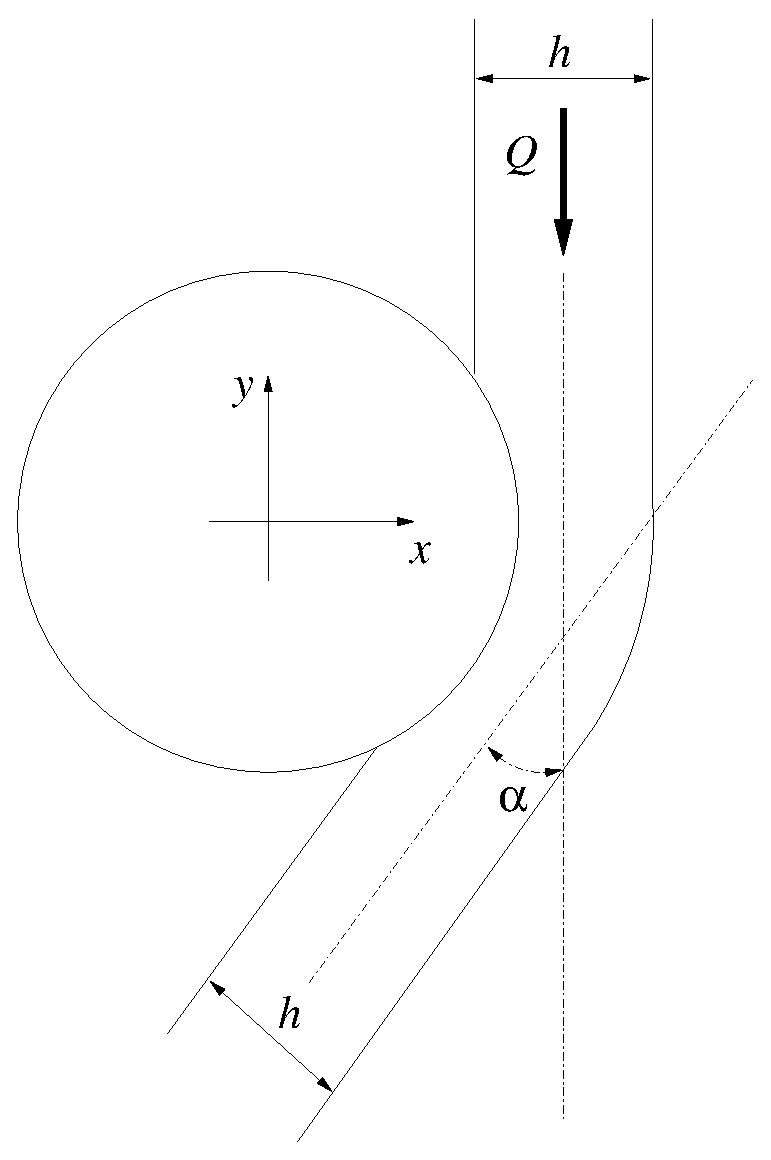
\includegraphics[width=0.90\textwidth]{./fig/coanda.eps}
   \end{center}
\end{minipage}
\end{tabular}

\vspace{1.0cm}

\sol

\partone
  Bilanci integrali di massa e quantità di moto. Equazioni di equilibrio (equazioni fondamentali della dinamica classica). Principio di azione e reazione. Integrale della normale su una superficie chiusa è identicamente nullo. Effetto Coanda (esempio della bustina da té sotto il rubinetto).

\parttwo
Vengono fatte alcune ipotesi: il problema stazionario; attorno al getto e al solido, l'aria è in quiete con pressione uniforme $p_a$; il profilo di velocità è uniforme sulle sezioni del getto considerate nelle equazioni di bilancio.

Partendo dalle equazioni di bilancio per il volume di controllo $V_{f}$ occupato dal fluido,  rielaborando il termine degli sforzi di superficie sforzi di superficie, si ricava la risultante $\bm{R}$ agente sul solido in funzione del flusso di quantità di moto del fluido attraverso la superficie $S_{f} = \partial V_f$.

Innanzitutto viene ricavata l'espressione della risultante $\bm{R}$ agente sul solido. 
\begin{itemize}
 \item Vengono scritte le equazioni di bilancio per il fluido, considerando il volume $V_f$
   \begin{equation}
     \begin{cases}
       \dfrac{d}{d t} \displaystyle\int_{V_f} \rho + \oint_{S_f} \rho \bm{u} \cdot \hat{\bm{n}} = 0 & \qquad \text{(massa)} \\
       \dfrac{d}{d t} \displaystyle\int_{V_f} \rho \bm{u} + \oint_{S_f} \rho \bm{u} \bm{u} \cdot \hat{\bm{n}} =
        \oint_{S_f} \bm{t_n} = 0  
%        \oint_{\partial \Omega} p \hat{\bm{n}} - \oint_{\partial \Omega} \bm{s_n} = 0  
        & \qquad \text{(quantità di moto)}  %\Rb^{ext}
      \end{cases}
    \end{equation}
 \item Viene introdotta l'ipotesi di stazionarietà del fenomeno, $\frac{d}{dt}\equiv 0$.
 La risultante degli sforzi viene scritta come somma degli sforzi di pressione e degli sforzi viscosi, 
\begin{equation}
\begin{split}
% & \Rb = \oint_{S_{cyl}}  {\bm{t}}_{\bm{n}} = 
% \oint_{S_{cyl}}  {\bm{s}}_{\bm{n}} - \oint_{S_{cyl}} p {\hat{\bm{n}}}_{cyl} \\
 & \oint_{S_f} \rho \bm{u} \bm{u} \cdot \hat{\bm{n}} 
  = \oint_{S_{f}}  {\bm{t}}_{\bm{n}} = 
 \oint_{S_{f}}  {\bm{s}}_{\bm{n}} - \oint_{S_f} p {\hat{\bm{n}}}_{f} \ .
\end{split}
\end{equation}

%\begin{equation}
%  \Rb = \oint_{S_{cyl}} \bm{t_n} = 
%  \int_{S_{ext}} \bm{t_n} + \int_{S_{c}} \bm{t_n} = 
%  - \int_{S_{ext}} p \bm{n}_{cyl} + \int_{S_{c}} \bm{t_n} = 
%\end{equation}


\item Viene manipolato il termine degli sforzi di superficie. Il contorno $S_f$ del volume fluido viene scomposto come unione della superficie a contatto con il solido $S_{fs}$, delle superfici ``laterali'' $S_{f\ell}$ (attraverso le quali non c'è flusso di quantità meccaniche, poichè $\bm{u}\cdot\bm{\hat{n}} = 0$) a contatto con l'aria in quiete e le sezioni ``di ingresso'' $S_{f,1}$ e ``di uscita'' $S_{f,2}$ sulle quali la velocità è uniforme, utilizzate per i bilanci integrali per il volume fluido. Viene indicata con $\bm{\hat{n}_f}$ la normale uscente dal volume $V_f$.
Il contorno $S_s$ del solido viene scomposto come unione della superficie a contatto con il fluido $S_{sf}$ e della superficie $S_{s\ell}$ a contatto con l'aria in quiete. Viene indicata con $\bm{\hat{n}_s}$ la normale uscente dal volume $V_s$.
In questo modo, la superficie $S_{fs}$ coincide con la superficie $S_{sf}$, a meno della normale invertita, $\bm{\hat{n}_f} = \bm{\hat{n}_s}$. Su queste superfici, per il terzo principio della dinamica, lo sforzo ${\bm{t_n}}_{sf}$ agente sul solido dovuto al fluido è uguale e contrario allo sforzo ${\bm{t_n}}_{fs}$ agente sul fluido dovuto al fluido, ${\bm{t_n}}_{sf}=-{\bm{t_n}}_{fs}$.
 La superficie formata dall'unione $S_{f\ell} \cup S_{f,1} \cup S_{f,2} \cup S_{s\ell} =:S_{ext}$ è una superficie chiusa con normale uscente $\bm{\hat{n}}$ uguale a $\bm{\hat{n}_f}$ sulle prime tre superfici e uguale a $\bm{\hat{n}}$ su $S_{s\ell}$. Lo sforzo agente su $S_{ext}$ è uguale a $-p_a\bm{\hat{n}}$, poiché le superfici libere sono a contatto con aria in quiete con pressione $p_a$ e le traiettorie delle particelle rettilinee (senza curvatura\footnote{Vedi commento sull'equazione della quantità di moto e sulle traiettorie delle particelle}) sulle sezioni $S_{f,1}$ e $S_{f,2}$.
%Si indica con $S_f$ il contorno fluido: questo è costituito dall'unione del controno a contatto con il cilindro $S_c$ e quella "libera" $S_l$. Il contorno del cilindro $S_{cyl}$ è suddiviso nel contorno $S_c$ a contatto con il fluido e nel contorno libero $S_{c_l}$.

%Nei passaggi successivi si ricava il legame tra sforzi sul contorno del dominio fluido e la forza agente sul cilindro.
%Si usa le ipotesi che sulle superfici libere agisca solo la pressione ambiente. Si usa il fatto che l'integrale di una quantità costante per la normale su una superficie chiusa è nullo. Si usa infine il fatto che $\bm{n}=-\bm{n}_{cyl}$ (normali uscenti dai due domini, uguali e contrarie) e
%$\bm{t_n}=-\bm{t}_{\bm{n}_{cyl}}$ (sforzi agenti sulla superficie comune, uguali e contrari).


\begin{equation}
\begin{aligned}
  \oint_{S_f} \bm{t_n} & = 
  \int_{S_{f\ell}} \bm{t_n} + \int_{S_{f,1+2}} \bm{t_n} + \int_{S_{fs}} \bm{t_n} = & \text{($\bm{t_n} |_{S_{f\ell},S_{f,1+2}} = -p_a \bm{\hat{n}_f}$ )}\\
  & = - \int_{S_{f\ell}\cup S_{f,1+2}} p_a \bm{\hat{n}_f} + \int_{S_{fs}} \bm{t_n} = & \text{(somma e sottrazione di $\int_{S_{fs}} p_a \bm{\hat{n}_f}$)}\\
  & = \underbrace{- \int_{S_{f\ell}\cup S_{f,1+2}} p_a \bm{\hat{n}_f} - \int_{S_{fs}} p_a \bm{\hat{n}_f}}_{-\oint_{S_f} p_a \bm{\hat{n}_f}=0}
  + \int_{S_{fs}} p_a \bm{\hat{n}_f} + \int_{S_{fs}} \bm{t_n} = & \text{($\bm{\hat{n}_f} = -\bm{\hat{n}_s}$, ${\bm{t_n}}_{fs} = - {\bm{t_n}}_{sf}$ su $S_{fs}$)} \\
  & = - \int_{S_{sf}} p_a \bm{\hat{n}}_{s} - \int_{S_{sf}} {\bm{t_n}}_{sf} = &
   \text{($\oint_{S_s=S_{sf}\cup S_{s\ell}} p_a \bm{\hat{n}_s} = 0)$} \\
  & = + \int_{S_{s\ell}} p_a \bm{\hat{n}}_{s} - \int_{S_{sf}} {\bm{t_n}}_{sf} = &
   \text{(${\bm{t_n}}_s = -p_a\bm{\hat{n}_s}$ su $S_{s\ell}$} \\
  & = - \int_{S_{s\ell}} {\bm{t_n}}_{s} - \int_{S_{sf}} {\bm{t_n}}_{sf} = - \oint_{S_{s}} {\bm{t_n}}_{s} = \\
%  \text{($S_{cyl} = S_c \cup S_{c_l}$ e $\int_{S_{cyl}} p_a \bm{n} = 0$)}\\
%  & = \int_{{S_c}_l} p_a \bm{n}_{cyl} + \int_{S_c} \bm{t_n} = &
%  \text{($\bm{t}_{\bm{n}_{s}}|_{S_{c_l}} = -p_a \bm{n}_{cyl}$, $\bm{t}_{\bm{n}_{cyl}}|_{S_c} = - \bm{t_n}$)} \\
%  & = - \int_{{S_c}_l} \bm{t}_{\bm{n}_{cyl}} - \int_{S_c} \bm{t}_{\bm{n}_{cyl}} = \\
%  & = - \int_{S_{cyl}} \bm{t}_{\bm{n}_{cyl}} \\
  & = - \bm{R} \ ,
\end{aligned}
\end{equation}
dove $\bm{R}$ è la risultante degli sforzi di superficie agente sul solido. In questo esercizio è il contributo delle forze di volume (ad esempio il peso) agenti sul solido.
% \item Riscrittura integrali di contorno % della pressione
%
%\begin{equation}
%\begin{split}
%  & \oint_{S_{cyl}} p {\hat{\bm{n}}}_{cyl} = 
%   \int_{S_c} (p-p_0) {\hat{\bm{n}}}_{cyl}
%   + \oint_{S_{cyl}} p_0 {\hat{\bm{n}}}_{cyl} =
%   \int_{S_c} (p-p_0) {\hat{\bm{n}}}_{cyl} \\
%  & \oint_{S_{f}} p {\hat{\bm{n}}} = 
%   \int_{S_c} (p-p_0) {\hat{\bm{n}}}
%   + \oint_{S_{f}} p_0 {\hat{\bm{n}}} =
%   \int_{S_c} (p-p_0) {\hat{\bm{n}}} = - \int_{S_c} (p-p_0) {\hat{\bm{n}}}_{cyl}\\   
%\end{split}
%\end{equation}


%\item Le relazioni semplificate vengono inserite nelle equazioni di equilibrio; si può scrivere quindi:
%\begin{equation}
%\begin{split}
%  \Rb & = - \oint_{S_{cyl}} p {\hat{\bm{n}}}_{cyl} = 
%   - \oint_{S_{c}} (p-p_0) {\hat{\bm{n}}}_{cyl} = 
%   \oint_{S_{c}} (p-p_0) {\hat{\bm{n}}} = 
%   -\oint_{S_f} \rho \bm{u} \bm{u} \cdot \hat{\bm{n}}
%\end{split}
%\end{equation}

\item Sostituendo nell'equazione del bilancio della quantità di moto si ottiene:
\begin{equation}
  \bm{R} = - \oint_{S_f} \rho \bm{u} \bm{u} \cdot \hat{\bm{n}} 
\end{equation}

\item Considerando solo le superfici di $V_f$ attraverso le quali c'è un flusso non nullo di quantità di moto, la risultante delle forze diventa
\begin{equation}
 \bm{R} = - \int_{S_{f,1}} \rho \bm{u} \bm{u} \cdot \hat{\bm{n}} 
          - \int_{S_{f,2}} \rho \bm{u} \bm{u} \cdot \hat{\bm{n}} 
\end{equation}
dove le quantità all'interno degli integrali sono riferite alle superfici di integrazione.
Sulle sezioni $S_{f,1}$, $S_{f,2}$ la velocità è uniforme con modulo $U$ (dalla continuità, la velocità sulle due sezioni è uguale poichè l'area delle due sezioni è uguale) diretta lungo la linea media del getto. Le componenti cartesiane della risultante $\bm{R}$ sono  
\begin{equation}
\begin{split}
  & R_x = \frac{Q^2 H}{\rho h} \sin \alpha \\
  & R_y = - \frac{Q^2 H}{\rho h} (1-\cos \alpha) \ ,
\end{split}
\end{equation} 
 riferite agli assi rappresentati in figura.
% L'area della sezione è $A = H h$ e la portata per unità di larghezza è $Q = \rho U h$ (quindi $\rho U^2 A = \frac{Q^2 H }{\rho h}$).

%Si scrive l'equazione precedente in componenti, proiettando lungo gli assi:



\end{itemize}
 % cilindro (Coanda)
\newpage

\noindent
\begin{tabular}{cc}
\begin{minipage}{0.60\textwidth}
\begin{exerciseS}[Giochi d'acqua]
Un getto d'acqua ($\rho=999\ kg/m^3 $) stazionario, piano e verticale 
viene indirizzato su un oggetto di massa $M$, tenuto da esso in equilibrio.
 Il getto ha distribuzione di velocità uniforme $U$ lungo lo spessore $H$, 
 mentre la distribuzione sul bordo dell'oggetto è 
triangolare di spessore $h$ con velocità massima $V$. Si calcoli la velocità $V$
e la massa $M$ dell'oggetto supponendo che:
\begin{itemize}
  \item il fluido che circonda il getto e il solido \`e aria in quiete a
  pressione atmosferica di $P_a = 101325\  Pa$;
  \item si possa trascurare la gravità nel bilancio di quantità di moto, ma non
nell'equilibrio del corpo.
\end{itemize} 


($V = U H / h ; M = \rho U^2 H / g$)
\end{exerciseS}
\end{minipage}
&
\begin{minipage}{0.35\textwidth}
   \begin{center}
   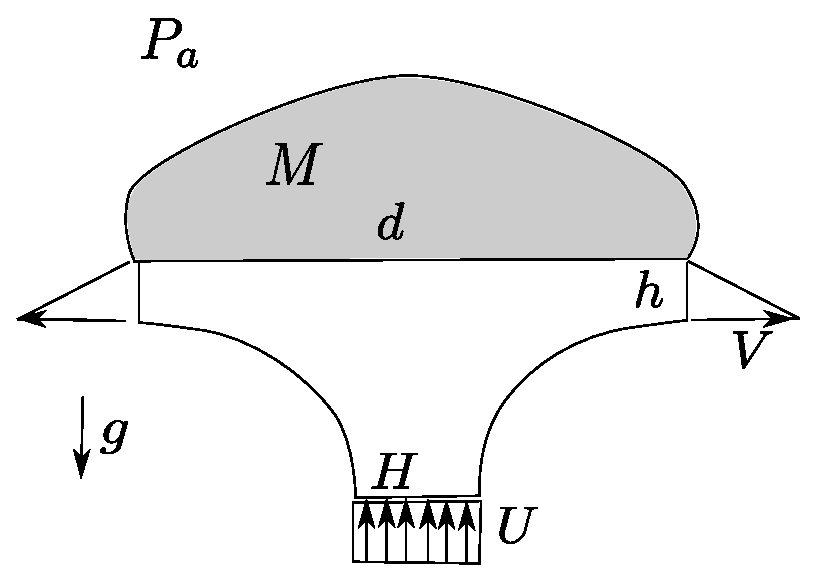
\includegraphics[width=0.90\textwidth]{./fig/gettoPiattello.eps}
   \end{center}
\end{minipage}
\end{tabular}

\vspace{1.0cm}

\sol

\partone
  Bilanci integrali di massa e quantità di moto. Equazioni di equilibrio (equazioni fondamentali della dinamica classica). Principio di azione e reazione. Integrale della normale su una superficie chiusa è identicamente nullo.

\parttwo
 Ipotesi: problema stazionario; sulla superficie libera del corpo e del fluido agisce solo la pressione ambiente $p_a$; nessun effetto della gravità nei bilanci del fluido.

Si sceglie un asse $y$ diretto verso l'alto.

\begin{itemize}
 \item Scrittura delle equazioni di bilancio per il fluido.
 
   \begin{equation}
     \begin{cases}
       \frac{d}{d t} \int_{\Omega} \rho + \oint_{\partial \Omega} \rho \bm{u} \cdot \hat{\bm{n}} = 0 & \qquad \text{(massa)} \\
       \frac{d}{d t} \int_{\Omega} \rho \bm{u} + \oint_{\partial \Omega} \rho \bm{u} \bm{u} \cdot \hat{\bm{n}} +
        \oint_{\partial \Omega} p \hat{\bm{n}} - \oint_{\partial \Omega} \bm{s_n} 
        -\int_V \rho \bm{g} = 0  
        & \qquad \text{(quantità di moto)}  %\Rb^{ext}
      \end{cases}
    \end{equation}

A queste, va aggiunta l'equazione di equilibrio del corpo sottoposto alla forza di gravità: $\bm{F} + M \bm {g} = 0$.

\item Dopo aver semplificato il bilancio di massa, da esso si ricava la velocità $V$. La velocità
 sui due
bordi 'di uscita' è $v(s) = V s/h$, avendo chiamato $s$ la coordinata che descrive tale superficie per valori compresi tra $0$ e $h$.
\begin{equation}
  0 = \int_{S_in} \rho \bm{u} \cdot \bm{\hat{n}} +   \int_{S_{out1}} \rho \bm{u} \cdot \bm{\hat{n}} +
  \int_{S_{out2}} \rho \bm{u} \cdot \bm{\hat{n}} = 
  - \rho U H + 2 \int_0^h \rho V \frac{s}{h} ds = \rho \displaystyle\left[
- U H + 2 \frac{1}{2} V h\right]
\end{equation}

E quindi $V = U \frac{H}{h}$.

 \item Le equazioni vengono opportunamente semplificate secondo le ipotesi fatte (vengono eliminati i termini non stazionari e il termine contenente le forze di volume - gravità). Il bordo del dominio fluido $\partial \Omega$ viene indicato con $S_f$. I contributi di pressione e viscosi vengono raccolti nel "vettore di sforzo" complessivo.


 
\begin{equation}
\begin{split}
% & \Rb = \oint_{S_{s}}  {\bm{t}}_{\bm{n}} = 
% \oint_{S_{s}}  {\bm{s}}_{\bm{n}} - \oint_{S_{s}} p {\hat{\bm{n}}}_{s} \\
 & \oint_{S_f} \rho \bm{u} \bm{u} \cdot \hat{\bm{n}}= 
 \oint_{S_{f}}  {\bm{s}}_{\bm{n}} - \oint_{S_f} p {\hat{\bm{n}}}
  = \oint_{S_{f}}  {\bm{t}}_{\bm{n}} 
\end{split}
\end{equation}


%\begin{equation}
%  \Rb = \oint_{S_{s}} \bm{t_n} = 
%  \int_{S_{ext}} \bm{t_n} + \int_{S_{c}} \bm{t_n} = 
%  - \int_{S_{ext}} p \bm{n}_{s} + \int_{S_{c}} \bm{t_n} = 
%\end{equation}


\item Riscrittura del termine di contorno. Si indica con $S_f$ il contorno fluido: questo è costituito dall'unione del controno a contatto con il corpo $S_c$ e quella "libera" $S_l$. Il contorno del corpo $S_{s}$ è suddiviso nel contorno $S_c$ a contatto con il fluido e nel contorno libero $S_{c_l}$.

Nei passaggi successivi si ricava il legame tra sforzi sul contorno del dominio fluido e la forza agente sul corpo.
Si usano le ipotesi che sulle superfici libere agisca solo la pressione ambiente. Si usa il fatto che l'integrale di una quantità costante per la normale su una superficie chiusa è nullo. Vengono
definite le normali $\bm{n}$ e $\bm{n_s}$ come la normale uscente dal volume del fluido e quella
uscente dal solido. Si definiscono $\bm{t}_{\bm{n}}$ e $\bm{t}_{\bm{n}_{s}}$ come lo sforzo agente sul fluido e quello agente sul solido. Si usa infine il fatto che $\bm{n}=-\bm{n}_{s}$ (normali uscenti dai due domini, uguali e contrarie) e
$\bm{t_n}=-\bm{t}_{\bm{n}_s}$ sulla superficie in comune (sforzi agenti sulla superficie comune, uguali e contrari; principio di azione e reazione).

\begin{equation}
\begin{aligned}
  \oint_{S_f} \bm{t_n} & = 
  \int_{S_l} \bm{t_n} + \int_{S_c} \bm{t_n} = & \text{($\bm{t_n} |_{S_l} = -p_a \bm{n}$ )}\\
  & = - \int_{S_l} p_a \bm{n} + \int_{S_c} \bm{t_n} = & \text{(somma e sottrazione di $\int_{S_c} p_a \bm{n}$)}\\
  & = \underbrace{- \int_{S_l} p_a \bm{n} - \int_{S_c} p_a \bm{n}}_{=0}
  + \int_{S_c} p_a \bm{n} + \int_{S_c} \bm{t_n} = & \text{($\bm{n} = -\bm{n}_{s}$)} \\
  & = - \int_{S_c} p_a \bm{n}_{s} + \int_{S_c} \bm{t_n} = &
  \text{($S_{s} = S_c \cup S_{c_l}$ e $\int_{S_{s}} p_a \bm{n} = 0$)}\\
  & = \int_{{S_c}_l} p_a \bm{n}_{s} + \int_{S_c} \bm{t_n} = &
  \text{($\bm{t}_{\bm{n}_{s}}|_{S_{c_l}} = -p_a \bm{n}_{s}$, $\bm{t}_{\bm{n}_{s}}|_{S_c} = - \bm{t_n}$)} \\
  & = - \int_{{S_c}_l} \bm{t}_{\bm{n}_{s}} - \int_{S_c} \bm{t}_{\bm{n}_{s}} = \\
  & = - \int_{S_{s}} \bm{t}_{\bm{n}_{s}} \\
  & = - \bm{R}
\end{aligned}
\end{equation}
% \item Riscrittura integrali di contorno % della pressione
%
%\begin{equation}
%\begin{split}
%  & \oint_{S_{s}} p {\hat{\bm{n}}}_{s} = 
%   \int_{S_c} (p-p_0) {\hat{\bm{n}}}_{s}
%   + \oint_{S_{s}} p_0 {\hat{\bm{n}}}_{s} =
%   \int_{S_c} (p-p_0) {\hat{\bm{n}}}_{s} \\
%  & \oint_{S_{f}} p {\hat{\bm{n}}} = 
%   \int_{S_c} (p-p_0) {\hat{\bm{n}}}
%   + \oint_{S_{f}} p_0 {\hat{\bm{n}}} =
%   \int_{S_c} (p-p_0) {\hat{\bm{n}}} = - \int_{S_c} (p-p_0) {\hat{\bm{n}}}_{s}\\   
%\end{split}
%\end{equation}


%\item Le relazioni semplificate vengono inserite nelle equazioni di equilibrio; si può scrivere quindi:
%\begin{equation}
%\begin{split}
%  \Rb & = - \oint_{S_{s}} p {\hat{\bm{n}}}_{s} = 
%   - \oint_{S_{c}} (p-p_0) {\hat{\bm{n}}}_{s} = 
%   \oint_{S_{c}} (p-p_0) {\hat{\bm{n}}} = 
%   -\oint_{S_f} \rho \bm{u} \bm{u} \cdot \hat{\bm{n}}
%\end{split}
%\end{equation}

\item Sostituendo nell'equazione del bilancio della quantità di moto si ottiene:
\begin{equation}
  \bm{R} = - \oint_{S_f} \rho \bm{u} \bm{u} \cdot \hat{\bm{n}} 
\end{equation}

\item Data la simmetria del problema si riconosce che non ci può essere una componente orizzontale.
I contributi nel bilancio della quantità di moto sulla superficie di contatto tra corpo e fluido e 
sulla superficie laterale del getto sono nulli poichè è nullo il flusso su tali superfici.
I contributi sulle sezioni 'di uscita' sono uguali e contrari. Rimane quindi solo il contributo 
dalla sezione 'in ingresso'.

\begin{equation}
  \bm{F} = - \oint_{S_f} \rho \bm{u} \bm{u} \cdot \bm{\hat{n}} = 
           - \oint_{S_in} \rho \bm{u} \bm{u} \cdot \bm{\hat{n}} = 
           \rho U^2 H \bm{\hat{y}}
\end{equation}

\item Si scrive l'equilibrio del corpo $\bm{F} + M \bm{g} = 0$, con $\bm{g} = - g \bm{\hat{y}}$.
Da questo segue che $M = F/g = \frac{\rho U^2 H}{g}$.

\end{itemize}


\textit{Osservazioni.} 
Nell'elaborazione dei termini della quantità di moto è contenuta la forma della risultante delle forze sull'oggetto vista in classe.

Come giustamente osservato da qualcuno in classe, la massa è per unità di lunghezza, poichè stiamo considerando un caso bidimensionale.
 % getto + piattello
\newpage
\noindent
\begin{tabular}{cc}
\begin{minipage}{0.60\textwidth}
\begin{exerciseS}[Motore a getto]
    Il motore a getto in figura è alimentato con una portata $\dot{m}_c = 
1.1\ kg/s$ di carburante liquido iniettato in direzione 
ortogonale all'asse del motore. Calcolare la spinta $T$ del 
motore ipotizzando che:
\begin{itemize}
\item il carburante vaporizzi e diffonda completamente;
\item le sezioni di ingresso e uscita abbiano area uguale e pari 
      ad $A = 0.5\ m^2$;
\item sia l'aria in ingresso che i gas di scarico siano a pressione 
    atmosferica $P_{atm}=26400\ Pa$;
\item la velocità di ingresso e di uscita siano uniformi sulle 
      rispettive sezioni;
\item siano note la densità dell'aria in ingresso $\rho_1 = 0.42\, 
      kg/m^3$, la velocità di ingresso $V_1 = 240\ m/s$ 
      e la velocità di efflusso $V_2 = 980\ m/s$.
\end{itemize}
($T = -38374\hat{\bm{x}}\ N$)
\end{exerciseS}
\end{minipage}
&
\begin{minipage}{0.35\textwidth}
   \begin{center}
   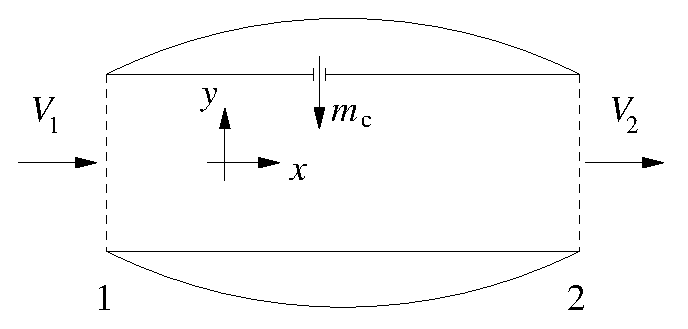
\includegraphics[width=0.90\textwidth]{./fig/motore_a_getto.eps}
   \end{center}
\end{minipage}
\end{tabular}

\sol
\begin{equation}
    T = \rho V_1 A (V_2-V_1) + V_2 \dot{m}_c \ .
\end{equation}

\partone
 Bilanci integrali di massa e quantità di moto.
\begin{equation}
\begin{cases}
  \frac{d}{dt} \int_V \rho = -\oint_{\partial V} \rho \bm{u} \cdot \hat{\bm{n}}  & \text{(massa)} \\
  \frac{d}{dt} \int_V \rho \bm{u} = -\oint_{\partial V} \rho \bm{u} \bm{u} \cdot \hat{\bm{n}}
  +\int_V \bm{f} - \oint_{\partial V} p \hat{\bm{n}} + \oint_{\partial V} \bm{s_n} & \text{(quantità di moto)}
\end{cases}
\end{equation}

\parttwo
Ipotesi: Regime stazionario. Fluido non viscoso (?). Profilo costante di velocità. No gravità.

\begin{itemize}
  \item Scrittura dei bilanci integrali con le semplificazioni opportune, derivanti dalle ipotesi.
    \begin{equation}
     \begin{cases}
      \oint_{\partial V} \rho \bm{u} \cdot \hat{\bm{n}} = 0  & \text{(massa)} \\
      \oint_{\partial V} \rho \bm{u} \bm{u} \cdot \hat{\bm{n}} = \oint_{\partial V} \bm{t_n} & \text{(quantità di moto)}
     \end{cases}
    \end{equation}
  \item Ulteriore semplificazione usando l'ipotesi di profili di velocità uniformi
    \begin{equation}
     \begin{cases}
      - \rho_1 V_1 A_1 -\dot{m}_c + \rho_2 V_2 A_2 = 0  \\
      - \rho_1 \vec{V_1} V_1 A_1 + \rho_2 \vec{V_2} V_2 A_2 - \dot{m}_c \vec{v}_c = \oint_{S1\cup S2\cup S3} \bm{t_n}
     \end{cases}
    \end{equation}
  \item Relazione tra l'integrale della pressione e la risultante delle forze agenti sul gomito, sfruttando il fatto che l'integrale della normale su tutta la superficie è identicamente nullo. Si identificano con $S_1$ la superficie di ingresso, $S_2$ la superficie di uscita, $S_3$ la superficie laterale interna del motore, $S_{3_o}$ la superficie laterale esterna del motore.
    \begin{equation}
     \begin{aligned}
      \displaystyle\oint_{S_1\cup S_2\cup S_3} \bm{t_n} & = \displaystyle\oint_{S_1\cup S_2\cup S_3} \bm{t_n} + \underbrace{\displaystyle\oint_{S_1\cup S_2\cup S{3_o}} p_a \hat{\bm{n}}}_{=0} = \\
      & = -\int_{S_1} (p-p_a) \hat{\bm{n}} - \int_{S_2} (p-p_a) \hat{\bm{n}} + \int_{S_{3_o}} p_a \hat{\bm{n}} + \int_{S_3} \bm{t_n}  = \qquad(p|_{S_1} = p|_{S_2} = p_a) \\
      & = \int_{S_{3_o}} p_a \hat{\bm{n}} + \int_{S_3} \bm{t_n} = \\
      & = \oint_{S_{eng}} \bm{t_n} = - \vec{F}
     \end{aligned}
    \end{equation}
  \item L'equazione della quantità di moto diventa quindi:
  \begin{equation}
  - \rho_1 \vec{V_1} V_1 A_1 + \rho_2 \vec{V_2} V_2 A_2 - \dot{m}_c \vec{v}_c = - \vec{F}
  \end{equation}
  \item Mettendo a sistema l'equazione del bilancio di massa e la proiezione in direzione orizzontale dell'equazione della quantità di moto (si assume che l'iniezione del combustibile, e quindi $\bm{v}_c$, sia perpendicolare all'asse x e quindi non compare nel bilancio della quantità di moto in direzione x):
  \begin{equation}
  \begin{cases}
    \rho_2 V_2 A = \rho_1 V_1 A + \dot{m}_c \\
    -\rho_1 V_1^2 A + \rho_2 V_2^2 A = -F_x 
  \end{cases}
  \end{equation}
  
  Si ottiene
  
  \begin{equation}
  \begin{aligned}
    F_x & = \rho_1 V_1^2 A - \rho_2 V_2^2 A = \\
        & = \rho_1 V_1^2 A - (\rho_2 V_2 A) V_2 = \\
        & = \rho_1 V_1^2 A - V_2 (\rho_1 V_1 A + \dot{m}_c) = \\
        & = \rho_1 V_1 A (V_1 - V_2) - V_2 \dot{m}_c
  \end{aligned}
  \end{equation}

  E la spinta coincide con la componente lungo x appena calcolata:
  \begin{equation}
    T = \rho_1 V_1 A (V_2 - V_1) + V_2 \dot{m}_c
  \end{equation}
  
  La spinta risulta quindi: $T = -F_x = 38374N$.
  
  \vspace{0.3cm}
  \textit{Interpretazione dei risultati e osservazioni.} 

In prima approssimazione, la spinta in un motore a getto è una funzione della portata d'aria e della differenza di velocità tra ingresso e uscita. Spesso in molte applicazioni il termine $\dot{m}_c$ è trascurabile.

Ragionare in questo caso sulla validità dell'approssimazione $\bm{t_n} = -p\bm{\hat{n}}$ nella 
definizione della risultante delle forze sul motore.


  
\end{itemize}
 % motore a getto (1)
\newpage
\noindent
\begin{tabular}{cc}
\begin{minipage}{0.60\textwidth}
\begin{exerciseS}[Gomito]
Un condotto di sezione circolare avente diametro $D = 5\ cm$ 
forma un gomito con angolo di $90^\circ$. Nel condotto scorre acqua ($\rho = 
999\ kg/m^3$) in regime stazionario con velocità $V = 
0.5\ rm m/s$. All'esterno del condotto vi è atmosfera con 
pressione uniforme $P_{atm}=101325\ Pa$; inoltre le pressioni 
all'ingresso e all'uscita del gomito sono uniformi sulla sezione ed 
entrambe pari a $P=10^6\ Pa$. Calcolare la forza $\bm{F}$ agente 
sul gomito.\\
($\bm{F} = -1765.03\hat{\bm{x}} + 1765.03\hat{\bm{y}}\  N$)
\end{exerciseS}
\end{minipage}
&
\begin{minipage}{0.35\textwidth}
   \begin{center}
   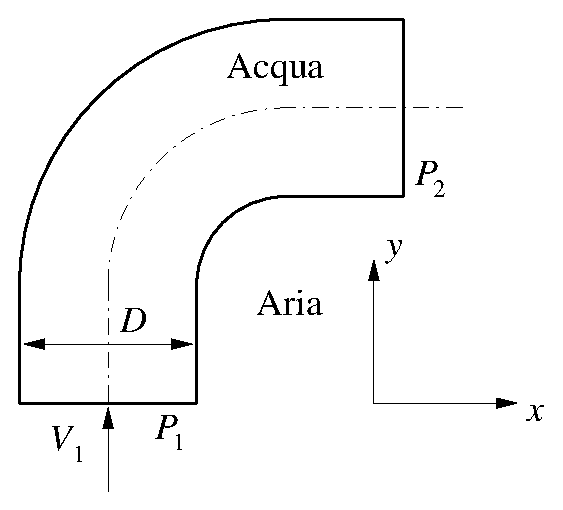
\includegraphics[width=0.70\textwidth]{./fig/gomito_01.eps}
   \end{center}
\end{minipage}
\end{tabular}


\sol

\partone
 Bilanci integrali di massa e quantità di moto. ...
\begin{equation}
\begin{cases}
  \frac{d}{dt} \int_V \rho = -\oint_{\partial V} \rho \bm{u} \cdot \hat{\bm{n}}  & \text{(massa)} \\
  \frac{d}{dt} \int_V \rho \bm{u} = -\oint_{\partial V} \rho \bm{u} \bm{u} \cdot \hat{\bm{n}}
  +\int_V \bm{F} - \oint_{\partial V} p \hat{\bm{n}} + \oint_{\partial V} {\bm{s_n}} & \text{(quantità di moto)}
\end{cases}
\end{equation}

\parttwo
Vengono fatte alcune ipotesi: regime stazionario, fluido incomprimibile, fluido non viscoso, profili costanti di velocità, no gravità.
Si scrivono i bilanci integrali semplificati, si riconoscono in essi e si calcolano le azioni scambiate con il corpo.

\begin{itemize}
  \item Scrittura dei bilanci integrali opportunamente semplificati (ipotesi).
    \begin{equation}
     \begin{cases}
      \oint_{\partial V} \rho \bm{u} \cdot \hat{\bm{n}} = 0  & \text{(massa)} \\
      \oint_{\partial V} \rho \bm{u} \bm{u} \cdot \hat{\bm{n}} = \oint_{\partial V} \bm{t_n} & \text{(quantità di moto)}
     \end{cases}
    \end{equation}
  \item Ulteriore semplificazione usando l'ipotesi di densità costante e profili di velocità uniformi
    \begin{equation}
     \begin{cases}
      -V_1 A_1 + V_2 A_2 = 0 \qquad \qquad \qquad \Rightarrow  V_1 = V_2 = V \\
      - \rho \vec{V_1} V_1 A_1 + \rho \vec{V_2} V_2 A_2 = \oint_{\partial V} \bm{t_n}
     \end{cases}
    \end{equation}
  \item Relazione tra l'integrale degli sforzi sulla superficie e la risultante delle forze agenti sul gomito, sfruttando il fatto che l'integrale della normale su tutta la superficie è identicamente nullo. Si identificano con $S_1$ la superficie di ingresso, $S_2$ la superficie di uscita, $S_3$ la superficie laterale.
    \begin{equation}
     \begin{aligned}
       \displaystyle\oint_{S_1\cup S_2\cup S_3} \bm{t_n} & =  \displaystyle\oint_{S_1\cup S_2\cup S_3} \bm{t_n} + \underbrace{\displaystyle\oint_{S_1\cup S_2\cup S_3} p_a \hat{n}}_{=0} = \\
      & = -\oint_{S_1} (p-p_a) \hat{n} - \oint_{S_2} (p-p_a) \hat{n} + \underbrace{\oint_{S_3} (\bm{t_n}+p_a \hat{n})}_{=-\bm{F}} =  \\
      & = -\oint_{S_1} (p-p_a) \hat{n} - \oint_{S_2} (p-p_a) \hat{n} - \bm{F} 
     \end{aligned}
    \end{equation}
  \item Proiezione lungo i due assi del sistema di riferimento della risultante delle forze agenti sul gomito (dopo averla inserita nell'equazione di bilancio della quantità di moto)
\begin{equation}
  \begin{cases}
    F_x = - \rho V^2 A - (p_2 - p_a)A   \\
    F_y =  \rho V^2 A + (p_1 - p_a)A  
  \end{cases}
  \end{equation}
%  \begin{equation}
%  \begin{cases}
%    F_x = - \rho V^2 A - (p_2 - p_a)A & \quad \Rightarrow \quad   F_x = -1765.03 N  \\
%    F_y =  \rho V^2 A + (p_1 - p_a)A  & \quad \Rightarrow \quad   F_y =  1765.03 N
%  \end{cases}
%  \end{equation}
\end{itemize}
 % gomito (1)
\newpage

\noindent
\begin{tabular}{cc}
\begin{minipage}{0.60\textwidth}
\begin{exerciseS}[Gomito]
Si consideri la corrente stazionaria nel gomito a 90$\,^\circ$ di una 
galleria a vento a circuito chiuso di cui è mostrata in figura la 
sezione nel piano $x$--$y$. Siano assegnate le aree della sezione di 
ingresso, $S_1 = 16 \ m^2$, e di uscita, $S_2 = 56 \ m^2$, 
la portata in volume $Q_1 = 1600 \  m^3/s$ e le pressioni nella 
sezione di ingresso, $P_1 = 1.05 \ bar$, e nella sezione di uscita, 
$P_2 = 1.106 \  bar$. Assumendo che il flusso d'aria sia incomprimibile 
($\rho = 1.225\ kg/m^3$) e che la velocità sulle sezioni di ingresso 
e uscita possa ritenersi uniforme, si determinino le componenti $F_x$ ed 
$F_y$ della spinta che esso esercita sul gomito, usando la convenzione 
indicata in figura.\\
($F_x = 1.876\,10^6\ N$, $F_y = -6.251\,10^6\ N$)
\end{exerciseS}
\end{minipage}
&
\begin{minipage}{0.35\textwidth}
   \begin{center}
   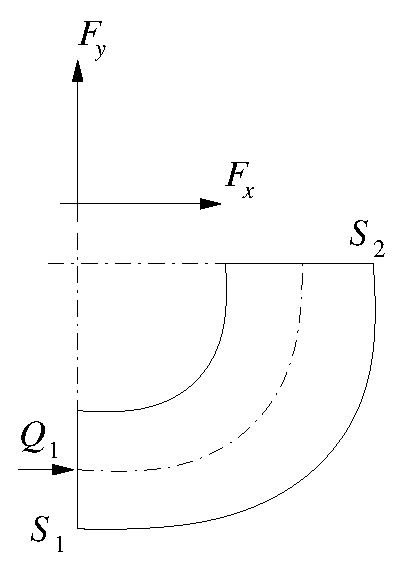
\includegraphics[width=0.60\textwidth]{./fig/gomito_galleria.eps}
   \end{center}
\end{minipage}
\end{tabular}


%%%%%%%%%%%%%%%%%%%%%%%%%%%%%%%%%%%%%%%%%%%%%%%%%%%%%%%%%%%%%%%%%%

\sol

\partone
  Bilanci integrali di massa e quantità di moto.
\begin{equation}
\begin{cases}
  \frac{d}{dt} \int_V \rho = -\oint_{\partial V} \rho \bm{u} \cdot \hat{\bm{n}}  & \text{(massa)} \\
  \frac{d}{dt} \int_V \rho \bm{u} = -\oint_{\partial V} \rho \bm{u} \bm{u} \cdot \hat{\bm{n}}
  +\int_V \bm{f} - \oint_{\partial V} p \hat{\bm{n}} + \oint_{\partial V} {\bm{t}_s} & \text{(quantità di moto)}
\end{cases}
\end{equation}



\parttwo
Vengono fatte alcune ipotesi: regime stazionario, fluido incomprimibile, fluido non viscoso, profili costanti di velocità, no gravità.
Si scrivono i bilanci integrali semplificati, si riconoscono in essi e si calcolano le azioni scambiate con il corpo.

\begin{itemize}
  \item Scrittura dei bilanci integrali con le semplificazioni opportune, derivanti dalle ipotesi.
    \begin{equation}
     \begin{cases}
      \oint_{\partial V} \rho \bm{u} \cdot \hat{\bm{n}} = 0  & \text{(massa)} \\
      \oint_{\partial V} \rho \bm{u} \bm{u} \cdot \hat{\bm{n}} = \oint_{\partial V} \bm{t_n} & \text{(quantità di moto)}
     \end{cases}
    \end{equation}
  \item Ulteriore semplificazione usando l'ipotesi di densità costante e profili di velocità uniformi
    \begin{equation}
     \begin{cases}
      -V_1 A_1 + V_2 A_2 = 0  & \quad \Rightarrow \quad V_1 A_1 = V_2 A_2 = Q \\
      - \rho \vec{V_1} V_1 A_1 + \rho \vec{V_2} V_2 A_2 = \oint_{\partial V} \bm{t_n}
     \end{cases}
    \end{equation}
  \item Relazione tra l'integrale della pressione e la risultante delle forze agenti sul gomito, sfruttando il fatto che l'integrale della normale su tutta la superficie è identicamente nullo. Si identificano con $S_1$ la superficie di ingresso, $S_2$ la superficie di uscita, $S_3$ la superficie laterale.
    \begin{equation}
     \begin{aligned}
      \displaystyle\oint_{S_1\cup S_2\cup S_3} p \hat{n} & =  \displaystyle\oint_{S_1\cup S_2\cup S_3} \bm{t_n} + \displaystyle\oint_{S_1\cup S_2\cup S_3} p_a \hat{n} = \\
      & = -\oint_{S_1} (p-p_a) \hat{n} - \oint_{S_2} (p-p_a) \hat{n} + \underbrace{\oint_{S_3} (\bm{t_n}+p_a\hat{n})}_{=-\bm{f}}  =  \\
      & = -\oint_{S_1} (p-p_a) \hat{n} - \oint_{S_2} (p-p_a) \hat{n} - \bm{f}
     \end{aligned}
    \end{equation}
  \item L'equazione della quantità di moto diventa quindi:
  \begin{equation}
  - \rho \bm{V_1} V_1 A_1 + \rho \bm{V_2} V_2 A_2 = - (p_1 - p_a) A_1 \hat{n}_1 - (p_2 - p_a) A_2 \hat{n}_2 - \bm{F}
  \end{equation}
  \item Proiezione lungo i due assi del sistema di riferimento della risultante delle forze agenti sul gomito.
  Se si considera $p_a = 0$, i risultati numerici sono i seguenti:
  \begin{equation}
  \begin{cases}
    F_x = \rho \frac{Q^2}{A_1} + (p_1 - p_a)A_1  & \quad \Rightarrow \quad   F_x = 1.876 \cdot 10^6 N  \\
    F_y = -  \rho \frac{Q^2}{A_2} - (p_2 - p_a)A_2  & \quad \Rightarrow \quad   F_y =-6.250 \cdot 10^6 N
  \end{cases}
  \end{equation}
\end{itemize}

 % gomito (2)

% todo: write the solution?
\newpage
\noindent
\begin{tabular}{cc}
\begin{minipage}{0.45\textwidth}
\begin{exerciseS}[Profili in schiera]
Un numero elevato di profili è disposto come in figura. Il profilo di ingresso
è uniforme $\bm{u} = U_\infty \bm{\hat{x}}$, mentre il profilo di uscita ha andamento
$\bm{u} = \beta U_\infty (\cos \theta \bm{\hat{x}} - \sin \theta \bm{\hat{y}})
\sin{\frac{\pi \eta}{H}}$ in ogni canale (sia $\eta$ la coordinata che descrive la
sezione di uscita).
Sulla sezione di ingresso la pressione media vale $P_1$, sulla sezione di uscita
 $P_2$. 

Calcolare il fattore $\beta$ del profilo di velocità in uscita e la risultante delle
 forze (per unità di apertura) agente sul singolo profilo.

(Risultati: $\beta = \frac{\pi}{2 \cos \theta}, \bm{F} = [(P_1 - P_2) H + \rho U^2 H ((1-\pi^2/8) ]\bm{\hat{x}} + \pi^2/8 \tan \theta \bm{\hat{y}}) $)
\end{exerciseS}
\end{minipage}
&
\begin{minipage}{0.50\textwidth}
   \begin{center}
   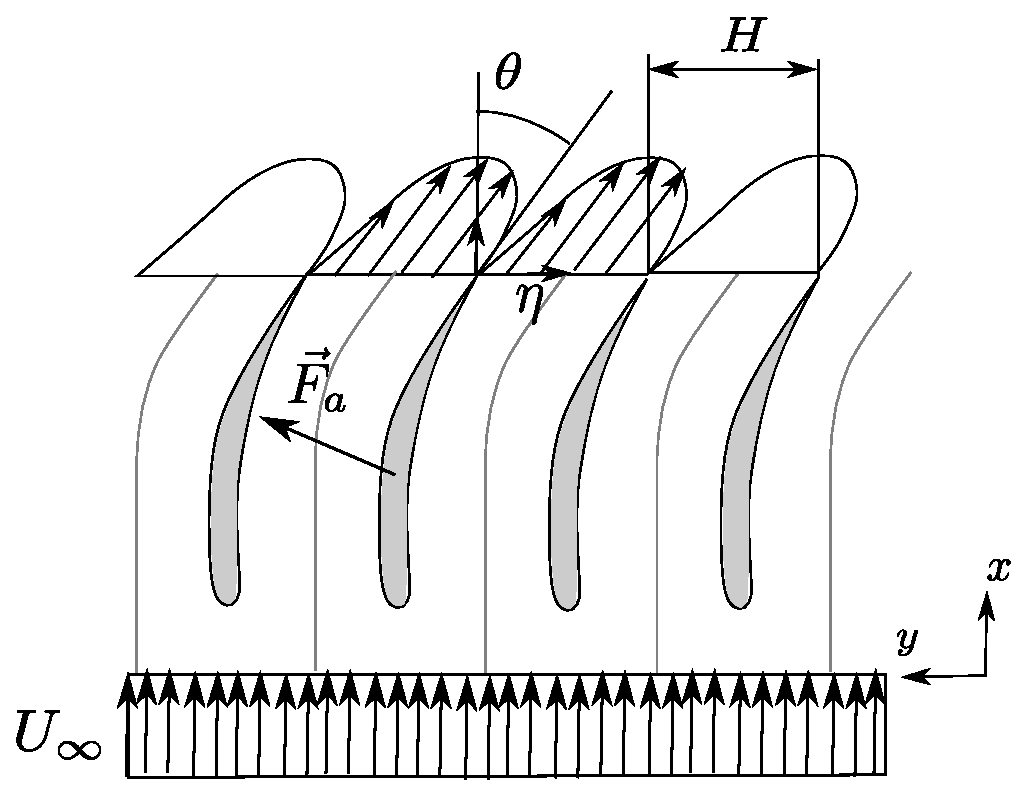
\includegraphics[width=0.95\textwidth]{./fig/wings.eps}
   \end{center}
\end{minipage}
\end{tabular}

\vspace{1.0cm}

\sol

\partone
  Bilanci integrali di massa e quantità di moto. Equazioni di equilibrio (equazioni fondamentali della dinamica classica). Principio di azione e reazione. Integrale della normale su una superficie chiusa è identicamente nullo. Simmetria.
\begin{itemize}
  \item Ricavare il coefficiente $\beta$ dal bilancio di massa
  \item Usare le ipotesi di simmetria nel bilancio di quantità di moto per annullare alcuni termini
\end{itemize} 

\parttwo

Si ricava il coefficiente $\beta$ dal bilancio di massa in forma integrale. Si utilizza la simmetria del problema nel bilancio di quantità moto per
 ricavare le azioni sui profili.

 % profili in schiera	

\newpage
\noindent
\begin{tabular}{cc}
\begin{minipage}{0.60\textwidth}
\begin{exerciseS}[Difetto di scia: stima resistenza]
Calcolare la resistenza di un profilo immerso in una corrente stazionaria 
con velocità asintotica ${\bm{V}}_\infty$, sapendo la distribuzione della 
componente di velocità $u(y)$ parallela a ${\bm{V}}_\infty$ a valle del 
profilo e assumendo che:
\begin{itemize}
\item la pressione statica sul contorno del volume di controllo
      sia costante e pari a quella della corrente indisturbata a monte
      del profilo;
\item sul lato superiore e inferiore del volume di controllo
      sia possibile trascurare la componente lungo l'asse $x$ della 
      perturbazione della velocit\`a dovuta alla presenza del profilo:
      $
      \bm{V} = (V_{\infty}+u,v) \simeq (V_{\infty},v).
      $
\end{itemize}
($R = \int_0^{ H}\rho \, u(y) [V_{\infty}-u(y)] dy.$)
\end{exerciseS}
\end{minipage}
&
\begin{minipage}{0.35\textwidth}
   \begin{center}
   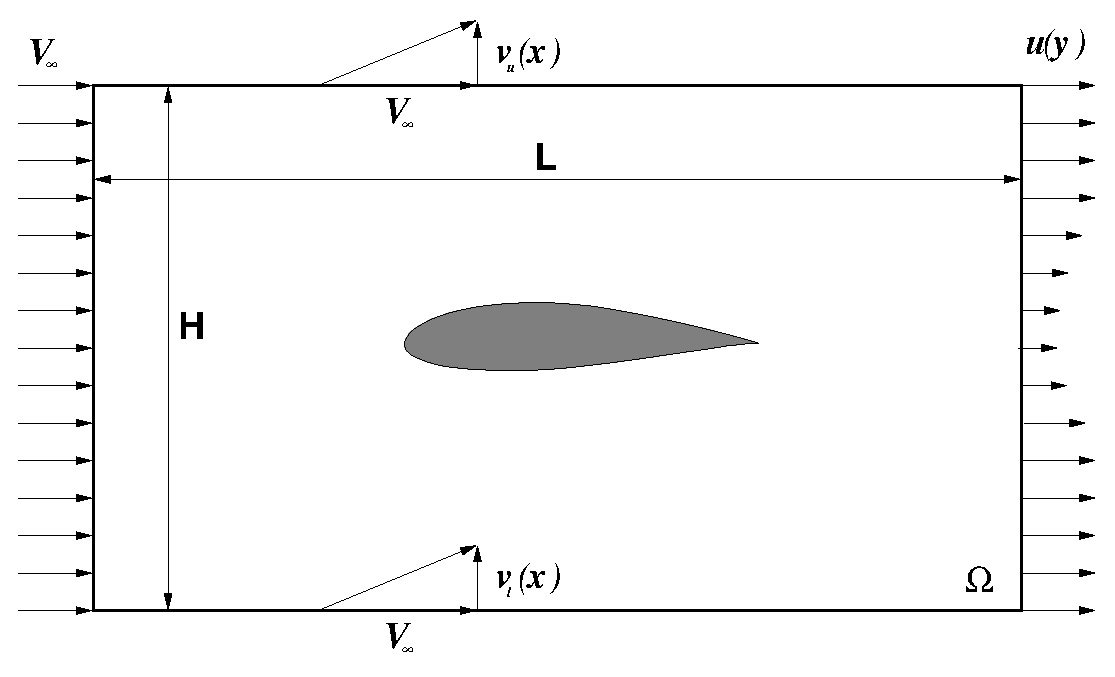
\includegraphics[width=0.90\textwidth]{./fig/airfoil.eps}
   \end{center}
\end{minipage}
\end{tabular}

\vspace{1.0cm}

\sol

\partone
  Bilanci integrali di massa e quantità di moto. Equazioni di equilibrio (equazioni fondamentali della dinamica classica). Principio di azione e reazione. Integrale della normale su una superficie chiusa è identicamente nullo. Esperienza in laboratorio sul \textit{difetto di scia}.

\parttwo
 Vengono scritti i bilanci integrali di massa e quantità di moto, opportunamente semplificati (ipotesi di stazionarietà $\frac{d}{dt} \equiv 0$, densità costante $\rho = \bar{\rho}$, ipotesi sulle condizioni sul bordo esterno del dominio); all'interno dei bilanci si possono riconoscere i termini legati alle azioni scambiate dal fluido con il profilo
 (l'incognita del problema); si sfrutta infine la geometria rettangolare del contorno esterno e le ipotesi su di esso per ottenere una forma ulteriormente semplificata dei bilanci e trovare la soluzione del problema.

\begin{itemize}
  \item Scrittura e semplificazione dei bilanci di massa e quantità di moto.
    \begin{equation}
      \begin{cases}
       \frac{d}{d t} \int_{\Omega} \rho + \oint_{\partial \Omega} \rho \bm{u} \cdot \hat{\bm{n}} = 0 & \qquad \text{(massa)} \\
       \frac{d}{d t} \int_{\Omega} \rho \bm{u} + \oint_{\partial \Omega} \rho \bm{u} \bm{u} \cdot \hat{\bm{n}} +
        \oint_{\partial \Omega} p \hat{\bm{n}} - \oint_{\partial \Omega} \bm{s_n} = 0  
        & \qquad \text{(quantità di moto)}  %\Rb^{ext}
      \end{cases}
    \end{equation}

%Dove $\Rb^{ext}$ è la risultante delle forze esterne che agiscono sul fluido. Nell'ipotesi che non ci siano altre forze esterne agenti sul fluido, se non quelle prodotte dal profilo, la forza $\bm{F}$ esercitata dal fluido sul profilo sarà uguale e contraria a $\Rb^{ext}$. L'incognita del problema è la resistenza del profilo, cioè la componente di $\bm{F}$ nella direzione della velocità asintotica $\Vb_{\infty}$ (in questo caso $F_x$).

Nel problema, il controno del dominio fluido $\partial \Omega$ è costituito dal bordo rettangolare $\gamma_\infty$ lontano dal profilo e dal bordo $\gamma_p$ coincidente con il profilo stesso. La forza $\bm{F}$ agente sul profilo è l'integrale degli sforzi generati dal fluido (uguali e contrari agli sforzi agenti sul fluido) sul contorno del profilo. Inoltre si può fare l'ipotesi di sforzi viscosi nulli e pressione costante sul bordo esterno: l'integrale sul dominio esterno si riduce all'integrale della normale su una superficie chiusa ed è quindi nullo. Si può dunque scrivere:
\begin{equation}
 \oint_{\partial \Omega} (-p \hat{\bm{n}} + \bm{s_n}) = \oint_{\partial \Omega} \bm{t_n} = \underbrace{\oint_{\gamma_p} \bm{t_n}}_{=-\bm{F}} + \underbrace{\oint_{\gamma_\infty} \bm{t_n}}_{=0} = -\bm{F}
\end{equation}

\textit{Osservazione. A differenza di quanto fatto in classe, non
è stata fatta l'ipotesi di fluido non viscoso; il contributo 
all'infinito si annulla con l'ipotesi di pressione costante 
all'infinito e sforzi viscosi trascurabili. Per ritrovarsi con gli appunti, sostituire $\bm{t_n}$ con
$-p\bm{\hat{n}}$}.

Dopo aver fatto l'ipotesi di stazionarietà e aver inserito la definizione di $\bm{F}$ appena data, le equazioni di bilancio possono essere scritte come:
    \begin{equation}
      \begin{cases}
      & \oint_{\partial \Omega} \rho \bm{u} \cdot \hat{\bm{n}} = 0  \\
      & \bm{F} = - \oint_{\partial \Omega} \rho \bm{u} \bm{u} \cdot \hat{\bm{n}} 
      \end{cases}
    \label{eqn:airfoil_bil_int}
    \end{equation}

Il bilancio di quantità di moto può essere scritto esplicitando e
separando le componenti vettoriali.
    \begin{equation}
    \begin{aligned}
       F_x\bm{\hat{x}} + F_y\bm{\hat{y}} 
& = - \oint_{\partial \Omega} \rho (u \bm{x} + v \bm{y}) \bm{u} \cdot \hat{\bm{n}} \\
& =       - \bm{\hat{x}} \oint_{\partial \Omega} \rho u \bm{u} \cdot \hat{\bm{n}} -  \bm{\hat{y}} \oint_{\partial \Omega} \rho v  \bm{u} \cdot \hat{\bm{n}}
    \end{aligned}
    \end{equation}
\item Scrittura delle equazioni di bilancio in componenti (sfruttando la geometria rettangolare del bordo esterno: $\gamma_1$ indica il bordo di sinistra, $\gamma_2$ il bordo inferiore, $\gamma_3$ quello di destra, $\gamma_4$ quello superiore).

\textit{Attenzione: la normale è quella uscente dal dominio fluido. Sul contorno del profilo, la
normale è entrante nel profilo. 
In più: non fare confusione tra azioni del profilo agenti sul fluido e azioni del fluido agenti 
sul profilo!}
  \begin{equation}
     \begin{cases}
      & 0 = \oint_{\partial \Omega} \rho \bm{u} \cdot \hat{\bm{n}} = -\int_{\gamma_1} \rho u
      -\int_{\gamma_2} \rho v +\int_{\gamma_3} \rho u +\int_{\gamma_4} \rho v \\
      & F_x = +\int_{\gamma_1} \rho u^2 +\int_{\gamma_2} \rho u v -\int_{\gamma_3} \rho u^2 -\int_{\gamma_4} \rho u v \\
      & F_y = +\int_{\gamma_1} \rho u v +\int_{\gamma_2} \rho v^2 -\int_{\gamma_3} \rho u v -\int_{\gamma_4} \rho v^2
     \end{cases}
  \end{equation}

\item Ipotesi sulla velocità sui lati orizzontali ($u|_{\gamma_2} = u|_{\gamma_4} = V_\infty$ costante), per poter ulteriormente semplificare il risultato.
   \begin{equation}
     \begin{cases}
        \int_{\gamma_2} \rho v  -\int_{\gamma_4} \rho v = -\int_{\gamma_1} \rho u+\int_{\gamma_3} \rho u\\
       F_x = +\int_{\gamma_1} \rho u^2 -\int_{\gamma_3} \rho u^2 + V_\infty \left[ \int_{\gamma_2} \rho v  -\int_{\gamma_4} \rho v \right]
     \end{cases}
  \end{equation}
E inserendo la prima nella seconda:
\begin{equation}
  \begin{aligned}
       F_x  & = \int_{\gamma_1} \rho u^2 -\int_{\gamma_3} \rho u^2 + V_\infty \left[-\int_{\gamma_1} \rho u+\int_{\gamma_3} \rho u \right] = \\
       & = \int_{\gamma_1} \rho u (u-V_\infty) + \int_{\gamma_3} \rho u (V_\infty-u) = \quad \text{($u|_{\gamma_1} = V_\infty  \Rightarrow $ il primo integrale è nullo)} \\
       & = \int_{\gamma_3} \rho u (V_\infty-u) = \\
       & = \int_{0}^{H} \rho u(y) (V_\infty - u(y)) dy
  \end{aligned}
\label{eqn:difetto_scia}
\end{equation}

\end{itemize}

\noindent
\textbf{Osservazioni.} Tramite la misura del campo di velocità in
galleria è possibile stimare la resistenza del corpo.
Le condizioni di ``aria libera'' e in galleria sono diverse. In generale, in galleria il fluido è confinato dalle pareti di galleria, maggiormente ``vincolato''. Inoltre sulle pareti della galleria esiste una condizione di adesione, $\bm{u}=\bm{0}$: per la conservazione della massa, il rallentamento del fluido in corrispondenza delle pareti della galleria viene compensato da un incremento della velocità nella regione ``più lontana'' dalla parete, rispetto a un corpo in aria libera.
 Per tenere conto di effetti di 
\textbf{bloccaggio} dovuti al confinamento in galleria, è necessario compiere delle correzioni delle misure sperimentali.
Agli effetti di bloccaggio, vanno aggiunti gli effetti di \textbf{galleggiamento} dovuti al gradiente di pressione lungo la galleria, che danno un effetto di resistenza aggiuntiva.
Inoltre è importante che la dimensione del corpo rispetto alla dimensione della galleria non sia né ``troppo grosso'' (per problemi di 'bloccaggio'), né, di solito, ``troppo piccolo'' (per motivi di similitudine; ma sarà argomento di puntate successive del corso...). \'E importante avere in mente la necessità di prestare attenzione a questi aspetti, quando vengono svolte attività sperimentali. Ma questo sarà argomento di altri capitoli o di altri corsi...


 % difetto di scia
% Stima resistenza (replica esperimento in galleria)
\subsection{Attività sperimentale: difetto di scia e volume di controllo.}

L'esercizio svolto in precedenza risulta propedeutico per l'analisi dei dati ottenuti tramite alcune attività sperimentali, per ottenere delle risultanti di forze e momenti da misure del campo di velocità (e pressione, a volte) tramite i bilanci integrali.
Le attività svolte nel mondo reale sono affette da imprecisioni e incertezze. La quantificazione (o almeno la stima) dell'incertezza del risultato di un'attività sperimentale è parte integrante del risultato stesso. 
I valori $x_i, \ i=1:N$ di grandezze misurate possono essere combinati per calcolare delle grandezze derivate $f(x_i)$. I \textit{datasheet} che accompagnano uno strumento raccolgono anche le informazioni sulla sua incertezza di misura, spesso in forma di intervallo di confidenza o di scarto quadratico medio. L'incertezza sulle misure sperimentali $x_i$ si propaga sul valore della funzione $f(x_i)$. Nell'ipotesi che le incertezze di misura sulle variabili $d_i$ siano tra di loro indipendenti e non correlate, è possibile utilizzare la \textbf{formula RSS} (\textbf{root-sum-squares}) per la propagazione dell'incertezza. Se la misura $x_i$ ha incertezza $\sigma_{x_i}$, una stima dell'incertezza su $f$ vale
\begin{equation}
  \sigma_f^2 = \sum_{i=1}^{N} \left( \dfrac{\partial f}{\partial x_i} \right)^2 \sigma_{x_i}^2 \ .
\end{equation}
%
L'incertezza $\sigma^2_f$ sulla quantità $f$, obiettivo dell'attività sperimentale, è un indicatore della bontà del metodo sperimentale utilizzato ed del sistema di miusra disponibile per tale attività. In generale, l'incertezza sulla grandezza desiderata deve essere ``molto minore'' della grandezza stessa: in caso contrario, l'apparato sperimentale risulterebbe indeguato all'esperimento.
Essendo parte integrante del risultato, è buona regola indicare l'incertezza sui risultati delle attività sperimentali, ad esempio fornendone il valore numerico, il valore relativo alla misura o gli intervalli di confidenza sui grafici.

% \paragraph{Difetto di scia e resistenza del profilo.}
% \'E possibile stimare la resistenza di un profilo a partire dalla misura del difetto di scia.
%  La misura di velocità in scia viene effettuata (con una sonda di Pitot o altro \dots)
%  in punti discreti, più radi lontano dalla scia del profilo,
%  fiù fitti in corrispondenza della scia dove i gradienti sono maggiori.
% L'integrale nella formula (\ref{eqn:difetto_scia}) viene approssimato con un metodo numerico,
%  come ad esempio la formula del punto medio, quella del trapezio, \dots
% Utilizzando qui per semplicità la formula del punto medio, è possibile scrivere
% \begin{equation}
%  F_x = \int_{0}^{H} \rho u(y) (U_\infty - u(y)) dy
%     \approx \sum_{k=1}^{N} \rho \left[ u_k (U_\infty - u_k) \right] \Delta s_k
% \end{equation}
% Le misure ottenute dalla sonda sono affette da incertezza $\sigma_{u_i}$; la derivata $\partial F_x / \partial u_i$ è
% \begin{equation}
%  \dfrac{\partial F_x}{\partial u_m}  = \rho \left( U_\infty - 2 u_m \right) \Delta s_m
% \end{equation}
% La stima dell'incertezza sulla resistenza è quindi
% \begin{equation}
%  \sigma_{F_x}^2 = \sum_{i=1}^{N} \left[ \rho \left( U_\infty - 2 u_i \right) \Delta s_i \right]^2 \sigma_{u_i}^2
% \end{equation}
% 

\paragraph{Risultante delle forze: bilancio di quantità di moto di un volume di controllo .}
Esistono metodi sperimentali, come ad esempio la \textbf{PIV} (Particle Image Velocimetry o, in italiano, velocimetria a immagini di particelle), che permettono di ottenere il campo di velocità in un determinato istante all'interno di un dominio di misura, un piano bidimensionale o un volume tridimensionale.
Il bilancio di quantità di moto del volume di controllo contenente un corpo solido permette poi di calcolare la risultante delle forze scambiate tra corpo e fluido.

\noindent
 Per semplicità, viene considerato un campo di moto bidimensionale, $\bm{u}(x,y)=u(x,y)\bm{\hat{x}}+v(x,y)\bm{\hat{y}}$. Ad esempio, il campo di moto attorno alla mezzeria di un'ala allungata senza freccia investita da una corrente con un angolo di incidenza ridotto è in buona approssimazione bidimensionale.
 In questo caso, misure PIV (PIV-2D-2C) forniscono le due componenti (2C) del campo di velocità nel piano (2D) di misura. Tramite il bilancio della quantità di moto del dominio bidimensionale, è possibile ottenere una stima della risultante delle forze (per unità di apertura) che esercita il fluido sul profilo di ala tagliato dal piano di misura.
Considerando gli effetti viscosi trascurabili, al di fuori di regioni di dimensione ridotta nell'ambito di applicazioni aeronautiche (alto numero di Reynolds, strato limite e scie sottili), il bilancio integrale della quantità di moto del fluido nel volume di misura fornisce, in un caso stazionario, la risultante delle forze ${\bm{R}}$ agenti sul corpo, 
\begin{equation}
 \bm{R} = -\oint_S \rho \bm{u} \bm{u} \cdot \bm{\hat{n}} - \oint_S p \bm{\hat{n}} \ ,
\end{equation}
avendo trascurato il contributo delle forze di volume.
%
Nell'ipotesi, più che sensata per molte applicazioni aeronautiche, che sia valido il teorema di Bernoulli sulla frontiera $S$ del volume di controllo, la pressione viene espressa in funzione della velocità locale e dello stato della corrente asintotica,
\begin{equation}
 p = p_\infty + \rho \dfrac{|\bm{U_\infty}|^2}{2} - \rho \dfrac{|\bm{u}|^2}{2} \ .
\end{equation}
Inserendo questa espressione della pressione nell'espressione della risultante delle forze ed eliminando gli integrali (nulli) su una superficie chiusa delle quantità costanti moltiplicate per la normale alla superficie, come ad esempio $\oint_S p_\infty \bm{\hat{n}}$, si può esprimere la risultante $\bm{R}$ della forza aerodinamica agente sul corpo in funzione della sola velocità del fluido sulla frontiera $S$,
\begin{equation}
 \bm{R} = -\oint_S \rho \bm{u} \bm{u} \cdot \bm{\hat{n}} + \oint_S \rho \dfrac{|\bm{u}|^2}{2} \bm{\hat{n}} \ .
\end{equation}
Sotto queste ipotesi, la forza aerodinamica agente sul corpo, in questo esempio l'obiettivo della misura, è stata scritta unicamente come funzione del campo di velocità sulla superficie $S$, fornito come ``risultato diretto'' dell'attività seprimentale. Per semplicità, la densità del fluido viene considerata costante e nota senza incertezza: nel caso che anche il campo di densità fosse affetto da incertezza, la formula RSS permette di aggiungere abbastanza facilmente il suo effetto a quello dovuto all'incertezza sulla misura del campo di velocità.
\newline
% TODO: è possible applicare diversi metodi per ricavare un'approssimazione della risultante e della sua incertezza, partendo da dati discreti...
\paragraph{Risultante delle forze: discretizzazione.}
Per la sua natura, la PIV fornisce dei risultati discreti (non continui): di solito, il campo di velocità viene misurato sui nodi di una griglia cartesiana. Per il calcolo della risultante $\bm{R}$ sono necessari solamente gli $N_n$ nodi esterni $\bm{x_i}, \ i=1:N_n$, posti sul contorno della griglia.
% TODO ...
\newline
Il campo di velocità viene approssimato (linearmente, per semplicità) utilizzando un approccio simile a quello impiegato nella modellazione numerica a elementi finiti. Viene introdotto un insieme completo di funzioni di base $\phi_i(\bm{x}), \ i=1:N_{n}$, lineari a tratti sul contorno $S$, grazie alle quali è possibile scrivere l'approssimazione $\bm{u}^h$ del campo di velocità
\begin{equation}\label{exp:u:fem-exp}
 \bm{u}(\bm{x}) \approx \bm{u}^h(\bm{x}) = \displaystyle\sum_{i=1}^{N_n} \phi_i(\bm{x}) \bm{U_i} \ . 
\end{equation}
Utilizzando funzioni di base lagrangiane, per le quali il valore della funzione $i$-esima $\phi_i(\bm{x})$ è uguale a uno sul nodo $i$-esimo $\bm{x}_i$ e zero sugli altri nodi,
\begin{equation}
 \phi_i(\bm{x_j}) = \delta_{ij} \qquad , \qquad \displaystyle\sum_{i=1}^{N_n} \phi_i(\bm{x}) = 1  \ , \forall i=1:N_n \ ,
\end{equation}
i coefficienti $\bm{U_i}$ della (\ref{exp:u:fem-exp}) concidono con i valori nodali, $\bm{U_i}:=\bm{u}(\bm{x_i})$ ricavati nei punti $\bm{x_i}$ tramite la misura sperimentale. Introducendo il campo di velocità approssimato $\bm{u}^h(\bm{x})$ nell'espressione della risultante delle forze, si ottiene una formula nella quale compaiono gli integrali di superficie del prodotto delle funzioni di base e del versore normale, 
\begin{equation}\label{eqn:RU}
\begin{aligned}
 \bm{R} \approx \bm{R}^h & = -\oint_S \rho \bm{u}^h \bm{u}^h \cdot \bm{\hat{n}} + \oint_S \rho \dfrac{\bm{u}^h \cdot \bm{u}^h}{2} \bm{\hat{n}} = \\
 & = - \rho \sum_{i=1}^{N_n} \sum_{j=1}^{N_n} \bm{U}_i \bm{U}_j \cdot \oint_S \phi_i(\bm{x}) \phi_j(\bm{x}) \bm{\hat{n}}(\bm{x})  + \dfrac{1}{2} \rho \sum_{i=1}^{N_n} \sum_{j=1}^{N_n}\bm{U}_i \cdot \bm{U}_j \oint_S  \phi_i(\bm{x}) \phi_j(\bm{x}) \bm{\hat{n}}(\bm{x}) = \\ 
 & = - \rho \sum_{i=1}^{N_n} \sum_{j=1}^{N_n} \bm{U}_i \bm{U}_j \cdot \bm{I}_{ij}  + \dfrac{1}{2} \rho \sum_{i=1}^{N_n} \sum_{j=1}^{N_n}\bm{U}_i \cdot \bm{U}_j \bm{I}_{ij} \ , 
\end{aligned}
\end{equation}
dove sono stati introdotti i vettori $\bm{I}_{ij} = \oint_S  \phi_i(\bm{x}) \phi_j(\bm{x}) \bm{\hat{n}}(\bm{x})$, facilmente calcolabili in maniera analitica, come spiegato nella sezione \S\ref{sec:fem}. \newline

% -------
\paragraph{Sensitività della risultante al campo di velocità.}
Per ricavare tramite la formula RSS l'incertezza sulla misura della risultante delle forze $\bm{R}$ dall'incertezza sulle misure del campo di velocità $\bm{u}(\bm{x})$, è necessario calcolare la \textit{variazione} di $\bm{R}$ rispetto al campo $\bm{u}(\bm{x})$. Perturbando il campo di velocità $\bm{u}(\bm{x})$ con la variazione $\delta \bm{u}(\bm{x})$, e trascurando i termini di ordine superiore al primo, dopo aver sottratto l'equazione ``non perturbata'', si ottiene la perturbazione della risultante delle forze $\delta \bm{R}$,
\begin{equation}\label{eqn:sens:cont}
\begin{aligned}
  \bm{R} + \delta \bm{R} & = -\oint_S \rho (\bm{u}+\delta\bm{u}) (\bm{u}+\delta\bm{u}) \cdot \bm{\hat{n}} + \oint_S \dfrac{1}{2}\rho (\bm{u}+\delta\bm{u}) \cdot (\bm{u}+\delta\bm{u}) \bm{\hat{n} } \\
  \rightarrow \delta \bm{R} & = -\oint_S \rho \left[ \bm{u} \bm{\hat{n}} \cdot \delta\bm{u} + \bm{u} \cdot \bm{\hat{n}} \delta\bm{u}\right]  + \oint_S \rho \bm{\hat{n}} \bm{u} \cdot \delta\bm{u} \\
 & = \oint_S \rho \left[ - \bm{u} \otimes \bm{\hat{n}} - (\bm{u} \cdot \bm{\hat{n}})\mathbb{I} + \bm{\hat{n}} \otimes \bm{u} \right] \cdot \delta\bm{u} = \\
 & = \oint_S \bm{\nabla}_u \bm{R} \cdot \delta\bm{u} = \\
 & =\oint_S \begin{bmatrix} \nabla_u R_x &  \nabla_v R_x \\ \nabla_u R_y &  \nabla_v R_y  \end{bmatrix} \cdot \begin{bmatrix} \delta u \\ \delta v \end{bmatrix} =
 \oint_S \begin{bmatrix} \bm{\nabla}_{\bm{u}} R_x \cdot \delta \bm{u} \\ \bm{\nabla}_{\bm{u}} R_y \cdot \delta \bm{u} \end{bmatrix} \ ,
\end{aligned}
\end{equation}
avendo introdotto il campo tensoriale della sensitività $\bm{\nabla}_{u} \bm{R}(\bm{x})$ della risultante delle forze rispetto al campo di velocità $\bm{u}(\bm{x})$ ed evidenziato l'influenza delle due componenti del campo di velocità sulle due componenti di forza. L'equazione precedente può essere scritta con notazione indiciale
\begin{equation}
 \qquad \delta R_i = \oint_S \nabla_{u_j} R_i \delta u_j = -\rho \oint_S \left[ u_i n_j + u_k n_k \delta_{ij} - n_i u_j \right] \delta u_j \ ,
\end{equation}
o esplicitamente in coordinate cartesiane, per ricavare l'espressione della sensitività della componenti della forza dalle singole componenti del campo di velocità,
\begin{equation}\label{eqn:sens:cart:simple}
\begin{aligned}
  \qquad & \begin{cases}
  \delta R_x & = \rho \displaystyle\oint_S \left[ -u n_x - u n_x - v n_y + u n_x \right] \delta u + \rho \oint_S \left[ -u n_y + v n_x   \right] \delta v \\
  \delta R_y & = \rho \displaystyle\oint_S \left[ -v n_x + u n_y \right] \delta u + \rho \oint_S \left[ -v n_y - u n_x - v n_y + v n_y \right] \delta v \\
\end{cases}  \vspace{5mm} \\
 \rightarrow & \begin{cases}
 \delta R_x & =
 \rho \displaystyle\oint_S \left[ -u n_x - v n_y \right] \delta u + \rho \oint_S \left[ -u n_y + v n_x   \right] \delta v =
 \oint_S \nabla_{u} R_x \ \delta u + \oint_S \nabla_v R_x \delta v \\
 \delta R_y & = \rho \displaystyle\oint_S \left[ -v n_x + u n_y \right] \delta u + \rho \oint_S \left[ -v n_y - u n_x \right] \delta v =
 \oint_S \nabla_{u} R_y \ \delta u + \oint_S \nabla_v R_y \delta v \ .
\end{cases}
\end{aligned}
\end{equation}

% ------
\paragraph{Sensitività della risultante alle misure di velocità.}
Partendo dall'espansione (\ref{exp:u:fem-exp}) del campo di velocità, la variazione del campo $\bm{u}^h(\bm{x})$ diventa
\begin{equation}\label{exp:du:fem-exp}
 \delta \bm{u}^h(\bm{x}) = \displaystyle\sum_{i=1}^{N_n} \phi_i(\bm{x}) \delta \bm{U}_i \ ,
\end{equation}
avendo indicato con $\delta \bm{U}_i$ la variazione dei valori nodali del campo di velocità. Le funzioni di base sono note, e quindi la loro variazione è nulla.\footnote{L'operazione di variazione ha proprietà simili a quelle di derivazione. Ad esempio la variazione del prodotto di due funzioni vale $\delta(ab) = \delta a \ b + a \ \delta b$.}
%
Introducendo l'espressione (\ref{exp:du:fem-exp}) di $\delta \bm{u}^h(\bm{x})$ all'interno della formula (\ref{eqn:sens:cont}) che lega la variazione $\delta \bm{R}$ alla variazione $\delta \bm{u}(\bm{x})$,
\begin{equation}
 \delta \bm{R} = \oint_S \bm{\nabla}_{\bm{u}} \bm{R} \cdot \delta \bm{u} 
  = \sum_{i=1}^{N_n} \oint_S \phi_i(\bm{x}) \bm{\nabla}_{\bm{u}} \bm{R} \cdot \delta \bm{U}_i  
 = \sum_{i=1}^{N_n} \bm{\nabla}_{\bm{U}_i} \bm{R} \cdot \delta \bm{U}_i \ ,
\end{equation}
 si ricava l'espressione della sensitività $\bm{\nabla}_{\bm{U}_i} \bm{R}$ della risultante delle forze rispetto alla misura di velocità $\bm{U}_i$, in funzione della sensitività $\bm{\nabla}_{\bm{U}_i} \bm{R}(\bm{x})$ della risultante rispetto al campo di velocità $\bm{u}(\bm{x})$ e alle funzioni di base $\phi_i(\bm{x})$,
\begin{equation}
 \bm{\nabla}_{\bm{U}_i} \bm{R} = \oint_S \phi_i(\bm{x}) \bm{\nabla}_{\bm{u}} \bm{R} \ .
\end{equation}
La sensitività $\bm{\nabla}_{\bm{U}_i} R_k$ della componente $R_k$ della risultante delle forze rispetto alla misura $\bm{U}_i$ è quindi
\begin{equation}
 \bm{\nabla}_{\bm{U}_i} R_k 
  = \oint_S \phi_i(\bm{x}) \bm{\nabla}_{\bm{u}} R_k \ . 
\end{equation}


\paragraph{Sensitività della risultante alle misure di velocità: discretizzazione.}
Inserendo l'approssimazione $\bm{u}^h$ nella formula della sensitività $\bm{\nabla}_{\bm{u}} \bm{R}$, è possibile calcolare la sensitività della risultante alle misure di velocità $\bm{U}_i$,
\begin{equation}\label{eqn:sens:RU}
\begin{aligned}
 \bm{\nabla}_{\bm{U}_i} \bm{R} & = \oint_S \phi_i(\bm{x}) \bm{\nabla}_{\bm{u}} \bm{R} =\\
 & = \oint_S \phi_i(\bm{x}) \rho \left[ - \bm{u} \otimes \bm{\hat{n}} - (\bm{u} \cdot \bm{\hat{n}})\mathbb{I} + \bm{\hat{n}} \otimes \bm{u} \right]  = \\
 & = \rho \displaystyle\sum_{j=1}^{N_n} \oint_S \phi_i(\bm{x}) \phi_j(\bm{x}) \left[ - \bm{U}_j \otimes \bm{\hat{n}} - (\bm{U}_j \cdot \bm{\hat{n}})\mathbb{I} + \bm{\hat{n}} \otimes \bm{U}_j \right]  = \\
 & = \rho \displaystyle\sum_{j=1}^{N_n} \left[ - \bm{U}_j \otimes \bm{I}_{ij} - (\bm{U}_j \cdot \bm{I}_{ij})\mathbb{I} + \bm{I}_{ij} \otimes \bm{U}_j \right] \ ,
\end{aligned}
\end{equation}
avendo riconosciuto i vettori $\bm{I}_{ij}$ definiti in precedenza. La sensitività della componente $R_k$ alla misura $\bm{U}_i$ vale
\begin{equation}
 \bm{\nabla}_{\bm{U}_i} R_k =  
  \rho \displaystyle\sum_{j=1}^{N_n} \left[ - U_{j,k} \bm{I}_{ij} - (\bm{U}_j \cdot \bm{I}_{ij}) \bm{\hat{e}}_k + I_{ij,k} \bm{U}_j \right] \ ,
\end{equation}
dove $\bm{\hat{e}}_k$ è il versore in direzione $k$ e $U_{j,k}$, $I_{ij,k}$ le componenti in quella direzione della misura $\bm{U}_i$ e del vettore $\bm{I}_{ij}$.

% {\color{red}
% Si può infine esprimere la sensitività in funzione del campo di velocità. La variazione $\delta \bm{R}$ è
% \begin{equation}
% \begin{aligned}
%  \delta \bm{R} & \approx - \rho \oint_S \left[ \bm{u}^h \bm{\hat{n}} \cdot \delta\bm{u}^h + \bm{u}^h \cdot \bm{\hat{n}}^h \delta\bm{u}\right] + \rho \oint_S \bm{\hat{n}} \bm{u}^h \cdot \delta\bm{u}^h = \\
%  & = - \rho \sum_{i=1}^{N_n} \sum_{j=1}^{N_n} \bm{U}_i \delta \bm{U}_j \cdot \oint_S \phi_i(\bm{x}) \phi_j(\bm{x}) \bm{\hat{n}}(\bm{x}) - \rho \sum_{i=1}^{N_n} \sum_{j=1}^{N_n} \delta\bm{U}_i \bm{U}_j \cdot \oint_S \phi_i(\bm{x}) \phi_j(\bm{x}) \bm{\hat{n}}(\bm{x}) + \\
%  & \hspace{6.7cm} + \rho \sum_{i=1}^{N_n} \sum_{j=1}^{N_n} \delta\bm{U}_i \cdot \bm{U}_j \oint_S  \phi_i(\bm{x}) \phi_j(\bm{x}) \bm{\hat{n}}(\bm{x}) = \\ 
%  & = - \rho \sum_{i=1}^{N_n} \sum_{j=1}^{N_n} \bm{U}_i \delta \bm{U}_j \cdot \bm{I}_{ij}  - \rho \sum_{i=1}^{N_n} \sum_{j=1}^{N_n} \delta \bm{U}_i \bm{U}_j \cdot \bm{I}_{ij} + \sum_{i=1}^{N_n} \sum_{j=1}^{N_n} \delta\bm{U}_i \cdot \bm{U}_j \bm{I}_{ij} \ , 
% \end{aligned}
% \end{equation}
% la cui componente $k$-esima è
% \begin{equation}
%  \delta R_k =  
%   - \rho \sum_{i=1}^{N_n} \sum_{j=1}^{N_n} U_{i,k} \delta \bm{U}_j \cdot \bm{I}_{ij}  - \rho \sum_{i=1}^{N_n} \sum_{j=1}^{N_n} \delta U_{i,k} \bm{U}_j \cdot \bm{I}_{ij} + \sum_{i=1}^{N_n} \sum_{j=1}^{N_n} \delta\bm{U}_i \cdot \bm{U}_j I_{ij,k} \ . 
% \end{equation}
% Sfruttando la simmetria rispetto agli indici dei vettori $\bm{I}_{ij}= \bm{I}_{ji}$, si possono invertire gli indici nella prima sommatoria per far comparire l'indice $i$ in tutti i termini con la variazione e scrivere
% \begin{equation}
%  \delta R_k =  
%   - \rho \sum_{i=1}^{N_n} \sum_{j=1}^{N_n} U_{j,k} \bm{I}_{ij}  \cdot \delta \bm{U}_i - \rho \sum_{i=1}^{N_n} \sum_{j=1}^{N_n} \bm{U}_j \cdot \bm{I}_{ij} \delta U_{i,k}  + \sum_{i=1}^{N_n} \sum_{j=1}^{N_n} I_{ij,k} \bm{U}_j \cdot \delta \bm{U}_i  \  
% \end{equation}
% e riconoscere la sensitività
% \begin{equation}
%  \bm{\nabla}_{\bm{U}_i} R_k =
%   - \rho \sum_{j=1}^{N_n} U_{j,k} \bm{I}_{ij} - \rho \sum_{j=1}^{N_n} \left(\bm{U}_j \cdot \bm{I}_{ij}\right) \ \bm{\hat{x}}_k  + \sum_{j=1}^{N_n} I_{ij,k} \bm{U}_j  \ , 
% \end{equation}
% avendo indicato con $\bm{\hat{x}}_k$ il versore nella $k$-esima direzione.
% }

\paragraph{Osservazione 1.} Si può dimostrare che le sensitività $\bm{\nabla}_{\bm{U_i}} \bm{R}$ sono le componenti del gradiente della formula (\ref{eqn:RU}) che esprime $\bm{R}$ come una funzione quadratica delle variabili $\bm{U}_i$.
% La formula (\ref{eqn:RU}) mostra che $\bm{R}$ è una funzione quadratica delle variabili $\bm{U}_i$. 
% La sua derivata rispetto alla variabile $\bm{U}_i$ vale
% \begin{equation}
%  -\rho \sum_{j=1}^{N_n} (\bm{U}_j \cdot \bm{I}_{ij} ) \mathbb{I} 
%  -\rho \sum_{j=1}^{N_n} (\bm{U}_{j} \otimes \bm{I}_{ij} ) 
%  +\rho \sum_{j=1}^{N_n} (\bm{I}_{ij} \otimes \bm{U}_{j} )   \ ,
% \end{equation}
% avendo sfruttato la proprietà $\bm{I}_{ij} = \bm{I}_{ji}$

\paragraph{Osservazione 2.} Utilizzando la formula generale (\ref{eqn:sens:RU}) o utilizzando la forma discretizzata delle espressioni (\ref{eqn:sens:cart:simple}), si può dimostrare che
\begin{equation}
\begin{aligned}
 \nabla_{U_{i,x}} R_x & = \nabla_{U_{i,y}} R_y = - \rho \displaystyle\sum_{j=1}^{N_n} \bm{U}_{j} \cdot \bm{I}_{ij} \\
 -\nabla_{U_{i,y}} R_x & = \nabla_{U_{i,x}} R_y = - \rho \displaystyle\sum_{j=1}^{N_n} \bm{U}_j  \times \bm{I}_{ij}\cdot \bm{\hat{z}} \\
\end{aligned}
\end{equation}

% -------
\paragraph{Incertezza sulla risultante dall'incertezza sulla misura di velocità.}
Utilizzando la formula del campo $\bm{u}^h$, viene calcolata la varianza $\sigma^2_{R_k}$ della componente $R_k$,
\begin{equation}
\begin{aligned}
 \sigma^2_{R_k} & = E[\delta R_k \delta R_k] = \rho^2 E\left[ \oint_{S(\bm{x})} \bm{\nabla}_{\bm{u}} R_k (\bm{x}) \cdot \delta \bm{u}(\bm{x}) \oint_{S(\bm{y})} \bm{\nabla}_{\bm{u}} R_k (\bm{y}) \cdot \delta \bm{u}(\bm{y}) \right] = \\
 & = \oint_{S(\bm{x})} \oint_{S(\bm{y})}  \bm{\nabla}_{\bm{u}} R_k (\bm{x}) \cdot E\left[ \delta \bm{u}(\bm{x}) \otimes \delta \bm{u}(\bm{y}) \right] \cdot \bm{\nabla}_{\bm{u}} R_k (\bm{y}) \approx \\
 & = \oint_{S(\bm{x})} \oint_{S(\bm{y})}  \bm{\nabla}_{\bm{u}} R_k (\bm{x}) \cdot \sum_{i=1}^{N_n} \sum_{j=1}^{N_n} \phi_i(\bm{x}) \phi_j(\bm{y}) E\left[ \delta \bm{U}_i \otimes \delta \bm{U}_j \right] \cdot \bm{\nabla}_{\bm{u}} R_k (\bm{y}) \ ,
\end{aligned}
\end{equation}
dove sono state indicate esplicitamente le variabili indipendenti $\bm{x}$, $\bm{y}$ sulle quali devono essere svolte le integrazioni.
\newline
Si fa l'ipotesi che l'incertezza della misura della componente in un punto sia indipendente dalla misura delle altre componenti della velocità nello stesso punto e dalla velocità negli altri punti del dominio. Si ipotizza inoltre che l'incertezza sulla singola misura in tutto il dominio sia uguale a $\sigma^2_U$ su tutte le componenti della velocità.
L'espressione dei valori attesi $E[\delta \bm{U}_i \otimes \delta \bm{U}_j]$ diventa quindi
\begin{equation}
  E[\delta \bm{U}_i \otimes \delta \bm{U}_j] = \sigma_U^2 \delta_{ij} \mathbb{I} 
\end{equation}
e di conseguenza l'incertezza della componente di forza $R_k$,
\begin{equation}
\begin{aligned}
 \sigma^2_{R_k} & = \oint_{S(\bm{x})} \oint_{S(\bm{y})}  \bm{\nabla}_{\bm{u}} R_k (\bm{x}) \cdot \sum_{i=1}^{N_n} \phi_i(\bm{x}) \phi_i(\bm{y}) \cdot \bm{\nabla}_{\bm{u}} R_k (\bm{y}) \sigma^2_U  = \\  
  & = \sum_{i=1}^{N_n}\left\{ \oint_{S(\bm{x})} \bm{\nabla}_{\bm{u}} R_k (\bm{x})   \phi_i(\bm{x}) \right\} \cdot \left\{ \oint_{S(\bm{y})} \bm{\nabla}_{\bm{u}} R_k (\bm{y}) \phi_i(\bm{y}) \right\} \sigma^2_U  = \\   
  & = \sum_{i=1}^{N_n} \bm{\nabla}_{\bm{U}_i} R_k \cdot \bm{\nabla}_{\bm{U}_i} R_k \ \sigma^2_U  = \\ 
  & = \sum_{i=1}^{N_n} | \bm{\nabla}_{\bm{U}_i} R_k |^2 \ \sigma^2_U = \\
  & = \sum_{i=1}^{N_n} \big( (\nabla_{U_{i,x}} R_k) ^2 + (\nabla_{U_{i,y}} R_k) ^2 \big) \ \sigma^2_U \ , 
\end{aligned}
\end{equation}
avendo riconosciuto la sensitività $\bm{\nabla}_{\bm{U}_i} R_k$ della componente di forza $R_k$ rispetto alla misura della velocità $\bm{U}_i = \bm{u}(\bm{x}_i)$.

%
\paragraph{Cenni sugli elementi finiti.}\label{sec:fem}
In questo paragrafo si fornisce qualche dettaglio sulla discretizzazione ``a elementi finiti'' usata nel calcolo della risultante aerodinamica e della sua incertezza.
Un dominio $S$, come ad esempio la superficie di controno del volume di controllo considerato, viene suddiviso negli elementi $S_k$, l'unione dei quali costituisce il dominio $S$
\begin{equation}
 S = \bigcup_{k=1}^{N_e} S_k
\end{equation}
 e che non hanno punti in comune tra di loro se non i bordi. Vengono poi definite delle funzioni di base $\phi_i(\bm{x})$, grazie alle quali è possibile approssimare (sulle quali viene proiettata) una funzione generica
\begin{equation}
 f(\bm{x}) = \displaystyle\sum_{i=1}^{N_n} \phi_i(\bm{x}) f_i \ .
\end{equation}
La dipendenza dalla variabile spaziale $\bm{x}$ è contenuta nelle funzioni di base $\phi(\bm{x})$, le quali vengono moltiplicate per i coefficienti $f_i$.
\newline
In generale, le funzioni $\phi_i(\bm{x})$ sono regolari a tratti, essendo regolari all'interno dei singoli elementi $S_k$ e continue sui loro bordi.
Nel metodo degli \textit{elementi finiti}, le funzioni di base sono \textit{a supporto compatto}, cioè sono diverse da zero solo su un dominio chiuso e limitato: il carattere ``locale'' delle singole funzioni di base viene sfruttato nel metodo degli elementi finiti per operare con matrici sparse, all'interno delle quali solo pochissimi elementi sono diversi da zero in ogni riga o colonna. Il supporto della funzione $\phi_i(\bm{x})$ è la parte di dominio al di di fuori della quale la funzione è nulla. Nel metodo degli elementi finiti, il supporto di $\phi_i(\bm{x})$ è costitutito dagli elementi $S_k$ ai quali appartiene il nodo $\bm{x}_i$. Indichiamo il supporto di $\phi_i(\bm{x})$ con $B_i$.
\newline
Le funzioni di base vengono definite lagrangiane, se la funzione $i$-esima $\phi_i(\bm{x})$ è uguale a uno sul nodo $i$-esimo $\bm{x}_i$ e zero sugli altri nodi,
\begin{equation}
 \phi_i(\bm{x}_j) = \delta_{ij} \qquad , \qquad \displaystyle\sum_{i=1}^{N_n} \phi_i(\bm{x}) = 1  \ , \forall i=1:N_n \ .
\end{equation}
In questo caso, i coefficienti $f_i$ concidono con i valori nodali della funzione $f(\bm{x})$, $f_i:=f(\bm{x_i})$.
Viene definita una \textit{connettività} della griglia degli elementi finiti, che consiste in un elenco ordinato dell'indice dei nodi di ogni elemento: in questa maniera viene definita una numerazione locale dei nodi di ogni singolo elemento, che risulta utile nel calcolo degli integrali. Viene indicato con $I_k = \{ i_{k1} , i_{k2} , \dots , i_{kn} \}$, l'elenco degli $n$ nodi dell'elemento $S_k$.

 In figura \ref{fig:base-fcn} è rappresentata una parte di una suddivisione in elementi finiti $S_{k}$ di un dominio monodimensionale, sul quale sono definite delle funzioni di base lagrangiane, lineari a tratti, a supporto compatto: ad esempio, la funzione di base $\phi_{i2}(\bm{x})$ è diversa da zero solo sugli elementi $S_{e1}$ e $S_{e2}$.
 Ogni elemento ha due nodi. Se viene definita la connettività nodi-elemento, 
\begin{equation}\label{eqn:conn:ex}
  \begin{aligned}
    I_{e1} = \{ i_1 , i_2 \} \ , \\
    I_{e2} = \{ i_2 , i_3 \} \ , \\
    I_{e3} = \{ i_4 , i_3 \} \ , \\
  \end{aligned}
\end{equation}
il nodo $i_1$ è il primo nodo (quello che ha l'indice $=1$ nella numerazione locale) dell'elemento $S_{e1}$, il nodo $i_2$ è il secondo nodo di $S_{e1}$ e il primo di $S_{e2}$, il nodo $i_3$ è il secondo nodo sia di $S_{e2}$ sia di $S_{e3}$, il nodo $i_4$ è il primo nodo di $S_{e3}$.

%
\begin{figure}[t]
 \centering
 \includegraphics[width=0.55\textwidth,trim=0 0 0 0]{./fig/base-functions} \hspace{20pt}
 \includegraphics[width=0.30\textwidth,trim=0 0 0 0]{./fig/base-functions-ref}
\caption{Esempio di funzioni di base lagrangiane lineari a tratti definite su un dominio monodimensionale.}\label{fig:base-fcn}
\end{figure}
%
 
Si utilizzano ora le proprietà della base di funzioni lineari a tratti $\phi_i(\bm{x})$ per calcolare i vettori $\bm{I}_{ij}$ che compaiono nel calcolo della risultante delle forze e nella sua varianza,
\begin{equation}
 \bm{I}_{ij} := \oint_S \phi_i(\bm{x}) \phi_j(\bm{x}) \bm{\hat{n}}(\bm{x}) \ .
\end{equation} 
Gli unici termini $\bm{I}_{ij}$ che non sono nulli sono quelli in cui compaiono due funzioni, che hanno supporti a intersezione non nulla, $B_i \cap B_j \neq 0$. In questi termini, il dominio di integrazione può essere limitato alla sola intersezione dei supporti delle due funzioni, essendo il prodotto di queste nullo al di fuori di esso. Ad esempio, facendo riferimento alla figura \ref{fig:base-fcn}, il termine $\bm{I}_{i2,i1}$ può essere riscritto come
\begin{equation}
 \bm{I}_{i2,i1} = \oint_S \phi_{i2}(\bm{x})\phi_{i1}(\bm{x})\bm{\hat{n}}   
                =  \int_{B_{i2}\cap B_{i1}} \phi_{i2}(\bm{x})\phi_{i1}(\bm{x})\bm{\hat{n}}   
                =  \int_{S_{e1}} \phi_{i2}(\bm{x})\phi_{i1}(\bm{x})\bm{\hat{n}} \ , 
\end{equation}
il termine $\bm{I}_{i2,i2}$ può essere riscritto come
\begin{equation}
 \bm{I}_{i2,i2} = \oint_S \phi_{i2}(\bm{x})\phi_{i2}(\bm{x})\bm{\hat{n}}   
                =  \int_{B_{i2}} \phi_{i2}(\bm{x})\phi_{i2}(\bm{x})\bm{\hat{n}}   
                =  \int_{S_{e1}\cup S_{e2}} \phi_{i2}(\bm{x})\phi_{i2}(\bm{x})\bm{\hat{n}} \ , 
\end{equation}
mentre il termine $\bm{I}_{i2,i4}$ è  nullo.
Gli integrali sugli elementi $S_i$ nello spazio ``fisico'' possono essere calcolati sull'elemento di riferimento $\hat{S}$, definito in $\xi \in [-1,1]$. La trasformazione di coordinate che porta l'elemento di riferimento $\hat{S}$ nell' elemento fisico $S_{k}$ delimitato dai punti di coordinata $x_{k1}$ e $x_{k2}$ è
\begin{equation}
 x = \dfrac{x_{k2}+x_{k1}}{2} + \dfrac{x_{k2}-x_{k1}}{2} \xi \ 
\end{equation}
e il suo ``determinante'' è
\begin{equation}
 \dfrac{\partial x}{\partial \xi} = \dfrac{x_{k2}-x_{k1}}{2} = \dfrac{\ell_k}{2} \ .
\end{equation}
Se si considera costante il versore normale $\bm{\hat{n}} = \bm{\hat{n}}_{S_{e1}}$ sull'elemento finito $S_{e1}$  e si utilizza la connettività nodi-griglia dell'esempio definita in (\ref{eqn:conn:ex}), l'integrale $\bm{I}_{i2,i1}$ può essere trasformato nell'integrale sull'elemento di riferimento
\begin{equation}
\begin{aligned}
 \bm{I}_{i2,i1} = \int_{S_{e1}} \phi_{i2}(x)\phi_{i1}(x)\bm{\hat{n}} dx & = \int_{\tilde{S}} \varphi_2(\xi) \varphi_1(\xi)  \dfrac{\partial x}{\partial \xi}  d\xi \ \bm{\hat{n}}_{S_{e1}} = \\
 & = \int_{\xi=-1}^{1}\varphi_2(\xi) \varphi_1(\xi)  \dfrac{\partial x}{\partial \xi}  d\xi \ \bm{\hat{n}}_{S_{e1}} \ , 
\end{aligned}
\end{equation}
 avendo riconosciuto il legame tra l'elemento $S_{e1}$ nel dominio fisico e quello di riferimento $\hat{S}$, $\phi_{i}(x) = \phi_i(x(\xi)) = \varphi_{i^{\ell}}(\xi)$, dove è stato indicato con $i^{\ell}$ l'indice locale del nodo globale con indice $i$: dalla connettività dell'elemento $S_{e1}$ risulta $i_1^\ell = 1$ $i_2^\ell = 2$.
Il ``determinante'' della trasformazione è noto e costante, $\partial x/\partial \xi|_{S_{e1}} = \ell_{S_{e1}}/2$. L'espressione delle funzioni sull'elemento locale è facilmente ricavabile. Le funzioni di base lagrangiane devono essere uguali a $1$ in un nodo e zero in tutti gli altri. Considerando i punti $\xi=-1$ e $x=1$ come primo e secondo nodo dell'elemento di riferimento $\hat{S}$, le funzioni definite sull'elemento di riferimento valgono
\begin{equation}
 \varphi_1(\xi) = \dfrac{1}{2}(1-\xi) \quad , \quad
 \varphi_2(\xi) = \dfrac{1}{2}(1+\xi) \ . 
\end{equation}
\'E immediato calcolare il valore degli integrali sull'elemento di riferimento,
\begin{equation}
\begin{aligned}
  \int_{-1}^{1} \varphi_1(\xi) \varphi_1(\xi) d\xi = \dfrac{2}{3} \quad & , \quad   
  \int_{-1}^{1} \varphi_1(\xi) \varphi_2(\xi) d\xi = \dfrac{1}{3} \\ 
  \int_{-1}^{1} \varphi_2(\xi) \varphi_1(\xi) d\xi = \dfrac{1}{3} \quad & , \quad   
  \int_{-1}^{1} \varphi_2(\xi) \varphi_2(\xi) d\xi = \dfrac{2}{3} \ .  
\end{aligned}
\end{equation}
Questi valori vengono infine utilizzati nel calcolo dei vettori $\bm{I}_{ij}$. I vettori dell'esempio valgono
\begin{equation}
\begin{aligned}
 \bm{I}_{i2,i1} & 
 = \int_{S_{e1}} \phi_{i2}(x)\phi_{i1}(x)\bm{\hat{n}} dx = \\ 
 & = \int_{\xi=-1}^{1}\varphi_2(\xi) \varphi_1(\xi)  \dfrac{\partial x}{\partial \xi}\bigg|_{S_{e1}}  d\xi \ \bm{\hat{n}}_{S_{e1}} = \dfrac{1}{3}\dfrac{\ell_{e1}}{2} \bm{\hat{n}}_{S_{e1}} = \dfrac{\ell_{e1}}{6} \bm{\hat{n}}_{S_{e1}}  \ , \\
 \bm{I}_{i2,i2} & = \int_{S_{e1}\cup S_{e2}} \phi_{i2}(x)\phi_{i2}(x)\bm{\hat{n}} \ dx = \\ 
 & = \int_{S_{e1}} \phi_{i2}(x)\phi_{i2}(x)\bm{\hat{n}} \ dx +    
     \int_{S_{e2}} \phi_{i2}(x)\phi_{i2}(x)\bm{\hat{n}} \ dx = \\ 
 & = \int_{\xi=-1}^{1}\varphi_2(\xi) \varphi_2(\xi)  \dfrac{\partial x}{\partial \xi}\bigg|_{S_{e1}}  d\xi \ \bm{\hat{n}}_{S_{e1}} + 
     \int_{\xi=-1}^{1}\varphi_1(\xi) \varphi_1(\xi)  \dfrac{\partial x}{\partial \xi}\bigg|_{S_{e2}}  d\xi \ \bm{\hat{n}}_{S_{e2}} = \\ 
 & = \dfrac{\ell_{e1}}{3} \bm{\hat{n}}_{S_{e1}} + \dfrac{\ell_{e2}}{3} \bm{\hat{n}}_{S_{e2}} \ . \\
\end{aligned}
\end{equation}


% old -----------------
% old -----------------
% old -----------------
% old -----------------
% {\color{red}
% \vspace{0.2cm}
% \textit{(In questa formula compare solo il termine di flusso di quantità di moto, mentre non è presente
%  il termine di sforzi di superficie $\oint_S \bm{t}_n$, che include il contributo della pressione, \textbf{non}
%  sempre trascurabile.)}
% \vspace{0.2cm}
% 
% Seguendo il procedimento svolto nel pragrafo precedente applicato all'integrale di superficie, è possibile
%  stimare l'incertezza sulla resistenza e sulla portanza ottenute tramite questo metodo.
% Si scopre che l'incertezza sulla misura dipende dalla risoluzione della griglia e dalle condizioni
%  di prova. Come indicazione generale, l'incertezza su portanza e resistenza sono dello stesso
%  ordine di grandezza, e possono raggiungere fino al $30\%$ della misura della resistenza.
% In molte applicazioni la portanza è maggiore della resistenza: in una prova ad efficienza del 
%  profilo $E=10$, si ottiene un $3\%$ di incertezza sulla portanza.
% In questo caso, questo metodo risulta accettabile per una stima della portanza, non per la resistenza.
% }






%> === Bilancio di energia ======================================
% galleria a circuito aperto
\newpage
\noindent
\begin{tabular}{cc}
\begin{minipage}{0.95\textwidth}
\begin{exerciseS}[Galleria a circuito aperto]
 Viene chiesto di determinare la potenza dei motori della galleria a circuito aperto rappresentata in figura, sapendo che la velocità massima desiderata nella sezione di prova è $V_{test} = 30 \, m/s$, l'area della sezione di prova è $A_{test} = 1.0 \, m^2$ e l'area della sezione in cui è alloggiato il ventilatore che mette in moto l'aria è $A_{fan} = 2.0 \, m^2$. Si supponga che la corrente sia incomprimibile e che la densità dell'aria sia $\rho = 1.1 \, kg/m^3$. In una prima fase, si trascuri la caduta di pressione attraverso il nido d'ape e gli schermi presenti tra la sezione 1 e la sezione 2 del condotto. Successivamente si ripeta il calcolo con una caduta di pressione $P_1 - P_2 = k \rho U^2$, con $k = \dots$.
\end{exerciseS}
\end{minipage}
\end{tabular}
\begin{figure}[h!]
 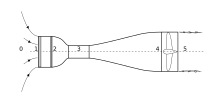
\includegraphics[width=0.90\textwidth]{./fig/wt}
\end{figure}

\sol

\partone
Si studia la galleria a circuito aperto rappresentata in figura utilizzando i bilanci integrali scritti per alcuni volumi di controllo fissi, per ricavare l'andamento della velocità e della pressione all'interno della galleria e infine ricavare la potenza dei motori, necessaria per garantire le condizioni di progetto nella sezione di prova. Si ipotizza un funzionamento stazionario, si trascurano gli effetti viscosi nel volume e sulle pareti della galleria e le forze di volume. In particolare, grazie alle ipotesi fatte, si possono semplificare il bilancio di massa,
\begin{equation}
\begin{aligned}
 & \dfrac{d}{dt} \int_V \rho = - \oint_{S} \rho \bm{u} \cdot \bm{\hat{n}} 
 \hspace{1.0cm} \rightarrow \hspace{1.0cm} \oint_{S} \rho \bm{u} \cdot \bm{\hat{n}} = 0 \ ,
\end{aligned}
\end{equation}
e il bilancio dell'energia cinetica,
\begin{equation}
\begin{aligned}
 \dfrac{d}{dt} \int_V \rho \dfrac{|\bm{u}|^2}{2} & = - \oint_{S} \rho \dfrac{|\bm{u}|^2}{2} \bm{u} \cdot \bm{\hat{n}} + \oint_S \bm{t_n} \cdot \bm{u} - \int_V \bm{\nabla} \bm{u} : \mathbb{T} + \int_V \rho \bm{g} \\
                                                 & = - \oint_{S} \rho \dfrac{|\bm{u}|^2}{2} \bm{u} \cdot \bm{\hat{n}} + \oint_S \bm{t_n} \cdot \bm{u} + 
 \underbrace{\int_V  p \, \bm{\nabla} \cdot \bm{u}}_{=0 \text{, se} \bm{\nabla} \cdot \bm{u} = 0}
 - \underbrace{ \int_V 2 \mu \mathbb{D} : \mathbb{D}}_{=0 \text{, se} \mu = 0} + \int_V \rho \bm{g} \\
 \hspace{1.0cm} \rightarrow \hspace{1.0cm}  &
 - \oint_{S} \rho \dfrac{|\bm{u}|^2}{2} \bm{u} \cdot \bm{\hat{n}} + \oint_S \bm{t_n} \cdot \bm{u} = 0 \ . 
\end{aligned}
\end{equation}

\parttwo
Viene svolta la prima parte dell'esercizio, trascurando le perdite di pressione che avvengono tra la sezione 1 e la sezione 2, a causa della presenza dei nidi d'ape e delle reti.
\newline \noindent
Si scrive il bilancio di massa per un volume di fluido che ha come superficie di contorno la superficie $S_0$, la superficie laterale del tubo di flusso e una superficie $S_i$ all'interno della galleria. Assumendo grandezze uniformi sulla sezione, si può scrivere
\begin{equation}
 \rho A_0 U_0 = \rho A_i U_i \ ,
\end{equation}
cioè che il flusso di massa $\dot{m}$ che attraversa le sezioni della galleria è costante. Se sono note le condizioni di progetto in camera di prova, da esser si può calcolare il flusso di massa,
\begin{equation}
 \dot{m} = \rho A_3 U_3 = \rho A_{test} V_{test} = \dots \ .
\end{equation}
Poiché la velocità all'infinito è nulla, $U_0 \rightarrow 0$, l'area della sezione all'infinito a monte deve tendere all'infinito $A_0 \rightarrow \infty$.
\newline \noindent
Si scrive poi il bilancio di energia cinetica per un volume di controllo che ha come contorno la superficie $S_0$ all'infinito a monte, dove viene aspirata l'aria in uno stato di quiete, la superficie laterale del tubo di flusso, la superficie interna della galleria e la sezione $S_4$ alla fine del divergente, poco prima dell'imbocco dei ventilatori. Poiché non ci sono organi meccanici in movimento, il termine $\oint_S \bm{t_n} \cdot \bm{u}$ è nullo, e assumendo grandezze fisiche costanti sulle sezioni si può scrivere,
\begin{equation}
 \rho A_0 U_0 \left( \dfrac{U_0^2}{2} + \dfrac{P_0}{\rho} \right) =
 \rho A_4 U_4 \left( \dfrac{U_4^2}{2} + \dfrac{P_4}{\rho} \right) \ .
\end{equation}
Poiché il flusso di massa che attraversa le sezioni considerate è costante, il bilancio di energia cinetica si riduce a un'espressione che ricorda quella del teorema di Bernoulli, così come viene enunciato alle scuole superiori,
\begin{equation}
 P_0 + \dfrac{1}{2} \rho \, U_0^2  = P_4 + \dfrac{1}{2} \rho \, U_4^2
 \qquad \rightarrow \qquad B_4 = B_0 = P_{atm} \ ,
\end{equation}
avendo introdotto la definizione del ``binomio di Bernoulli'', $B_i = P_i + \rho U_i^2 / 2$.
\newline \noindent
Si scrive poi il bilancio di energia cinetica per il volume fluido $V(t)$ che contiene il ventilatore, delimintato dalle superifci $S_4$, $S_5$ e la superficie interna della galleria e dalla superficie (mobile!) del ventilatore. Il bilancio diventa
\begin{equation}
\int_{S_4} \rho \dfrac{|\bm{u}|^2}{2} \bm{u} \cdot \bm{\hat{n}} - \bm{t_n} \cdot \bm{u} + 
\int_{S_5} \rho \dfrac{|\bm{u}|^2}{2} \bm{u} \cdot \bm{\hat{n}} - \bm{t_n} \cdot \bm{u} = \int_{S_{fan}} \bm{t_n} \cdot \bm{u} \ ,
\end{equation}
essendo il termine a destra dell'uguale la potenza delle forze essercitata dal ventilatore sul fluido, contraria a quella esercitata dal fluido sul ventilatore, ma uguale a quella che deve fornire il motore elettrico per poter garantire la rotazione del ventialore stesso. Se si trascurano gli sforzi viscosi sulle superfici $S_4$ ed $S_5$, $\bm{t_n} = \bm{s_n} - P \bm{\hat{n}}$, e se si esplicita la potenza che deve essere fornita dai motori, il bilancio diventa,
\begin{equation}
 W_{mot} = 
\int_{S_4} \left( \rho \dfrac{|\bm{u}|^2}{2} + P \right) \left( \bm{u} \cdot \bm{\hat{n}} \right)  + 
\int_{S_5} \left( \rho \dfrac{|\bm{u}|^2}{2} + P \right) \left( \bm{u} \cdot \bm{\hat{n}} \right) \ , 
\end{equation}
e facendo l'ipotesi di grandezze fisiche costanti sulle sezioni,
\begin{equation}
 W_{mot} = \rho A_5 U_5 \left( \dfrac{U_5^2}{2} + \dfrac{P_5}{\rho} \right) 
         - \rho A_4 U_4 \left( \dfrac{U_4^2}{2} + \dfrac{P_4}{\rho} \right)
         = \dot{m} \left( B_5 - B_4 \right) \ . 
\end{equation}
Ricordando che il ``binomio di Bernoulli'' nelle sezioni 1:4 è uguale al ``binomio di Bernoulli'' nella sezione $S_0$, e quindi uguale alla pressione ambiente $P_{atm}$, nell'ipotesi che la pressione nella sezione $S_5$ sia uguale alla pressione atmosferica $P_{atm}$ all'esterno del tubo di flusso, la potenza del motore diventa,
\begin{equation}
 W_{mot} = \dot{m} \dfrac{U_5^2}{2} \ ,
\end{equation}
e, riferendosi alle grandezze fisiche in camera di prova, può essere scritta come
\begin{equation}
\begin{aligned}
 & W_{mot} = \dot{m} \left( \dfrac{A_{test}}{A_{fan}} \right)^2 \dfrac{V_{test}^2}{2} \\
 & \hspace{3.0cm} \rightarrow \qquad 
 W_{mot} = \dfrac{1}{2} \rho A_{test} \left( \dfrac{A_{test}}{A_{fan}} \right)^2 V_{test}^3 = \dots kW \ .
\end{aligned}
\end{equation}
La formula della potenza dei motori necessaria al funzionamento della galleria mette in evidenza la dipendenza dal cubo della velocità di prova e dal quadrato del rapporto tra l'area della sezione di prova e l'area della sezione all'imbocco delle ventole. Questo ultimo termine dovrebbe chiarire uno degli obiettivi del divergente della galleria: rallentare la corrente dopo la sezione di prova, per poter ridurre la potenza dei motori da installare per garantire il funzionamento dell'impianto.
%
\newline \noindent
\textbf{Osservazione.} Potrebbe suscitare qualche perplessità il fatto che la corrente in uscita dall'impianto con velocità $U_5 \simeq V_{fan}$ abbia una pressione uguale alla pressione ambiente, $P_{atm}$, come il fluido in quiete all'esterno del tubo di flusso. {\color{red} Provando ad applicare il teorema di Bernoulli} tra un punto sulla sezione del tubo di flusso $S_5$ e un punto all'esterno del tubo di flusso,
{\color{red}
\begin{equation}
 P_5 + \dfrac{1}{2}\rho V_{fan}^2 = P_5^{out}
 \quad \rightarrow \quad 
 P_{atm} + \dfrac{1}{2}\rho V_{fan}^2 = P_{atm} \ ,
\end{equation}
}
si giungerebbe alla conclusione che {\color{red} $V_{fan} = 0$}. L'errore risiede nell'applicazione del teorema di Bernoulli nella formula vista alla scuola superiore (o in altri corsi universitari), nonostante alcune ipotesi (che verranno presentate nel prosieguo del corso) non siano rispettate. In particolare, per collegare un punto sulla sezione $S_5$ e un punto all'esterno del tubo di flusso viene attraversato uno strato di mescolamento tra la corrente in moto che esce dalla galleria e il fluido in quiete all'esterno: la presenza di questo strato di mescolamento, nel quale la corrente non è irrotazionale $\bm{\omega} \neq 0$, fa cadere le ipotesi del teorema di Bernoulli e lo rende quindi inapplicabile. Tutte {\color{red}le parti evidenziate in rosso devono quindi essere considerate errate}.


% ciclo Otto e potenza di un motore alternativo
\newpage
\noindent
\begin{tabular}{cc}
\begin{minipage}{0.95\textwidth}
\begin{exerciseS}[Motore alternativo]
Il funzionamento di un motore alternativo a benzina (a quattro tempi) può essere rappresentato in prima approssimazione con un ciclo termodinamico Otto ideale, rappresentato da una compressione adiabatica, una fase veloce di combustione a volume costante (nel punto morto superiore del moto del pistone, PMS) e un'espansione adiabatica. Le fasi di aspirazione e scarico dei gas combusti sono anch'essi ideali. L'aspirazione avviene a pressione costante durante il movimento del pistone dal PMS al punto morto inferiore (PMI). La fase di scarico avviene in due fasi: durante la prima fase la pressione diminuisce molto velocemente (approssimata da una trasformazione a volume costante) a causa dell'apertura della valvola di scarico quando il pistone si trova al PMI; durante la seconda fase i gas combusti sono spinti fuori dalla camera di combustione dal movimento ascendente del pistone che si riporta al PMS, per l'inizio del ciclo termodinamico successivo. Del motore sono noti:
\begin{itemize}
 \item il rapporto di compressione, definito come il rapporto tra il volume massimo (pistone al PMI) e minimo (pistone al PMS) della camera di combustione, $r = V_1 / V_2 = 10$;
 \item la cilindrata, definita come la corsa del pistone per l'area della sezione del cilindro, e uguale alla differenza $C = N (V_2 - V_1) = 1000 \ cc$, essendo $N$ il numero di cilindri del motore;
 \item le condizioni termodinamiche dell'aria all'aspirazione $P_0 = 85570 \, Pa$, $T_0 = 25°C$;
 \item il rapporto in massa tra benzina e aria, $f = m_f / m_a = 0.06$;
 \item il potere calorifico della benzina usata $\Delta h = 43 \, MJ$;
 \item la pressione nel basamento del motore, $p_{b} = 150000 \, Pa$ uniforme e costante.
Si calcoli la potenza media erogata dal motore a un regime di rotazione di $\Omega = 3000 RPM$, assumendo un rendimento meccanico $\eta = 0.8$.
Si rappresenti l'aria come un gas bi-atomico perfetto ($\gamma = c_P/ c_v = 1.4$) con costante dei gas $R = 287 J / (kg \, K)$, e si trascuri l'effetto del carburante sul valore dei calori specifici e sulla massa presente all'interno della camera di combustione. Si trascurino inoltre gli scambi di calore per conduzione con l'esterno del cilindro durante la compressione e l'espansione (trasformazioni adiabatiche). Si trascurino i termini cinetici nell'energia totale in camera di combustione, facendo coincidere l'energia totale con l'energia interna $e^t = e = c_v T$, e si assuma che le variabili termodinamiche siano uniformi (costanti in spazio, non in tempo) in camera di combustione.
\end{itemize}
\end{exerciseS}
\end{minipage}
\end{tabular}
\begin{figure}[h]
 \centering
 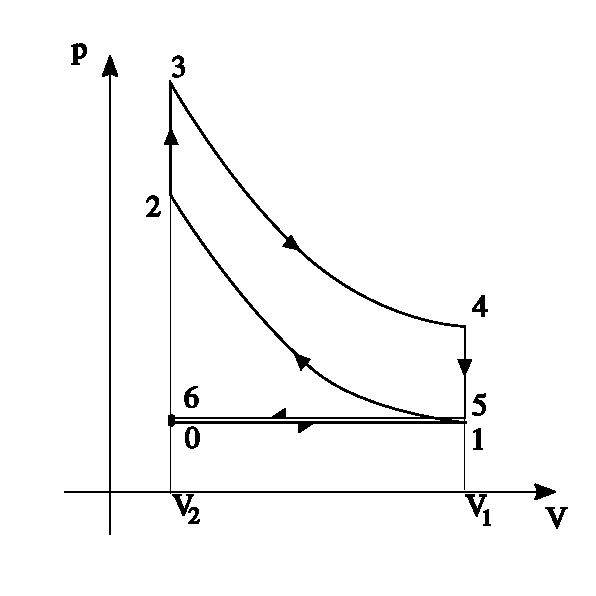
\includegraphics[width=0.45\textwidth]{./fig/otto_cycle}
\end{figure}

% todo: figure with the cut-out of the cylinder, thermodynamic cycle

%
\sol

% Concetti
\partone
Ogni fase del ciclo termodinamico viene analizzata con i bilanci integrali, per il volume corrispondente alla camera di combustione di un cilindro. Questo volume è un sistema aperto durante la fase di aspirazione e scarico (scambia massa con l'esterno), mentre è un sistema chiuso durante la compressione, la combustione e l'espansione (valvole chiuse, nessuno scambio di massa con l'esterno). Si calcola il lavoro svolto dal sistema durante un ciclo e si divide per il periodo per ricavare la potenza media. 

% Svolgimento
\parttwo
Conoscendo il numero dei cilindri $N=3$, il rapporto di compressione $r$ e la cilindrata $C$ è possibile ricavare il valore del volume massimo $V_1$ e minimo $V_2$ della camera di combustione.
\begin{equation}
\begin{cases}
 N( V_2 - V_1 ) = C \\
 V_1 / V_2 = r
\end{cases} \qquad \rightarrow \qquad
\begin{cases}
 V_1 = \dfrac{r}{r-1} \dfrac{C}{N} \\ \\ 
 V_2 = \dfrac{1}{r-1} \dfrac{C}{N}
\end{cases} 
\end{equation}
Si analizzano ora le fasi del ciclo termodinamico, fornendo una breve descrizione e ponendo attenzione allo scambio di massa (sistema chiuso/aperto), lavoro e calore con l'esterno.
\begin{itemize}
\item \textbf{Aspirazione}, $0 \rightarrow 1$: la prima fase del ciclo Otto è l'aspirazione. Durante la fase di aspirazione (ideale), la valvola di aspirazione è aperta e il sistema scambia massa con l'esterno: il pistone si sposta dal PMS al PMI e la camera di combustione si riempie d'aria a pressione e temperatura costante,
\begin{equation}
 p_1 = p_0 \qquad , \qquad
 T_1 = T_0 \qquad , \qquad
 \rho_1 = \rho_0 = \dfrac{p_0}{R T_0} =
\end{equation}
La massa contenuta nella camera di combustione alla chiusura della valvola, in coincidenza del PMI, è
\begin{equation}
 m = \rho_1 V_1 = \dots \ .
\end{equation}
Durante la fase di aspirazione, il pistone deve vincere la sovrapressione del basamento (di solito la pressione nel basamento è superiore a quella aspirata in camera di combustione). Dal PMS al PMI un pistone assorbe parte della potenza fornita dagli altri pistoni. Il lavoro che assorbe è $L_{01} = -(p_b-p_0) \, c$ (negativo poichè assorbito), essendo $c$ la corsa del pistone e la differenza di pressione costante durante l'aspirazione. Questo lavoro assorbito durante l'aspirazione sarà uguale e contrario a quello fornito durante lo scarico ideale dei gas,  che avviene alla stessa differenza di pressione con un moto opposto.
\item \textbf{Compressione}, $1 \rightarrow 2$: la seconda fase del ciclo termodinamico è la compressione del fluido che avviene a causa del movimento verso l'alto del pistone. Il sistema è chiuso: le valvole sono chiuse e si ipotizza che non ci sia trafilamento (\textit{blow-by}) tra il pistone e la superficie laterale del cilindro. Il bilancio di energia totale per il fluido contenuto all'interno del volume $V(t)$ (variabile nel tempo, a causa del moto del pistone) della camera di combustione,
\begin{equation}
 \dfrac{d}{dt} \displaystyle\int_{V(t)} \rho e^t + \oint_{S(t)} \rho e^t (\bm{u}-\bm{v}) \cdot \bm{\hat{n}}= \int_{V(t)} \bm{f} \cdot \bm{u} + \oint_{S(t)} \bm{t_n} \cdot \bm{u} - \oint_{S(t)} \bm{q} \cdot \bm{\hat{n}} + \int_{V(t)} \rho r \ .
\end{equation}
può essere semplificato, trascurando l'effetto delle forze di volume, $\bm{f} = \bm{0}$, trascurando la trasmissione del calore con l'esterno (trasformazione adiabatica), $\bm{q} \cdot \bm{\hat{n}} = 0$, e non essendoci sorgenti di calore, $r = 0$. Inoltre non c'è flusso di massa attraverso il contorno $S(t)$ del volume, $(\bm{u}-\bm{v}) \cdot \bm{\hat{n}} = 0$, e l'unica superficie in movimento della camera di combustione corrisponde al cielo (la faccia superiore) del pistone, $S_{c}$. Trascurando il contributo cinetico e approssimando l'energia totale $e^t = e + |\bm{u}|^2/2$ con l'energia interna $e$, il bilancio di energia diventa,
\begin{equation}
 \dfrac{d}{dt} \displaystyle\int_{V(t)} \rho e = \int_{S_c(t)} \bm{t_n} \cdot \bm{u} \ ,
\end{equation}
legando la derivata temporale dell'energia del fluido nella camera di combustione alla potenza delle forze esercitate dal pistone sul fluido. La potenza delle forze agenti sul pistone è uguale all'integrale superficiale del prodotto scalare vettore sforzo $\bm{t_{n,s}}$ agente sul solido per la velocità $\bm{v}$ della superficie del solido,
\begin{equation}
\begin{aligned}
 W_{12} = \oint_{S_{s}} \bm{t_{n,s}} \cdot \bm{v}
 & = \int_{S_{s,c}} \bm{t_{n,s}} \cdot \bm{v} + \int_{S_{s,b}} \bm{t_{n,s}} \cdot \bm{v}  + \int_{S_{s,lat}} \bm{t_{n,s}} \cdot \bm{v} = \\
 & = - \int_{S_{c}} \bm{t_{n}} \cdot \bm{u} - \int_{S_{s,b}} p_b\bm{\hat{n}_{s}} \cdot \bm{v} \ ,
\end{aligned}
\end{equation}
avendo suddiviso la superficie del cilindro $S_s$ come l'unione della superficie superiore $S_{s,c}$ (cielo), superficie laterale $S_{s,lat}$ (dal contributo nullo, per simmetria), e superifice inferiore $S_{s,b}$ esposta verso il basamento del motore, sulla quale agisce uno sforzo dovuto alla pressione $p_b$ dell'ambiente all'interno del basamento. \'E stato indicata con $\bm{\hat{n}_s}$ la normale uscente dalla superficie del solido e con $\bm{t_{n,s}}$ il vettore sforzo agente su un punto della superficie del solido, uguale e contrario a quello agente sul fluido $\bm{t_n} = -\bm{t_{n,s}}$ per il principio di azione e reazione. Inoltre, le condizioni al contorno impongono che il fluido e il solido abbiano la stessa velocità $\bm{u} = \bm{v}$ sulle superfici di contatto.
Si può quindi riscrivere il bilancio di energia del fluido in funzione della potenza $W_{12}$ trasmessa al pistone,
\begin{equation}
  \dfrac{d}{dt} \displaystyle\int_{V(t)} \rho e = - W_{12} - p_b S_{c} \ v(t) = - W_{12} - p_b \dfrac{d V}{d t} \ ,
\end{equation}
essendo $v(t)$ la velocità del pistone, per ottenere la potenza trasmessa al pistone dal fluido (sarà una potenza richiesta, $<0$),
\begin{equation}
\begin{aligned}
  W_{12}(t) & = - \dfrac{d}{dt} \displaystyle\int_{V(t)} \rho e - p_b \dfrac{d V}{d t} = \\
  & = - \dfrac{d}{dt} \left( \rho V e \right) - p_b \dfrac{d V}{d t} = \\
  & = - m \dfrac{d e}{d t} - p_b \dfrac{d V}{d t} \ ,
\end{aligned}
\end{equation}
nell'ipotesi di variabili termodinamiche uniformi nel volume, ricordando che la massa contenuta nella camera di combustione $m = \rho V$ rimane costante, essendo un sistema chiuso, se si trascura l'effetto di trafilamento tra le pareti di cilindro e pistone (ridotte al minimo da fasce elastiche e anelli raschiaolio sul pistone e sovra-pressione nel basamento).
\newline \noindent
Integrando in tempo la potenza istantantea $W_{12}(t)$, tra il punto 1 e il punto 2 del ciclo, si ottiene il lavoro di compressione
\begin{equation}
 L_{12} = - m (e_2 - e_1) - p_b ( V_2 - V_1 ) \ .
\end{equation}
Utilizzando la legge di stato dei gas perfetti $p = \rho R T$ e il legame tra le variabili termodinamiche durante una trasformazione adiabatica $p/\rho^\gamma = \text{cost}$, si ottiene
\begin{equation}
 e_2 - e_1 = c_v ( T_2 - T_1 ) = c_v T_1 \left[ \left( \dfrac{\rho_2}{\rho_1} \right)^{\gamma-1} - 1 \right] = c_v T_1 \left( r^{\gamma-1} - 1\right) \ .
\end{equation}

\item \textbf{Combustione}, $2 \rightarrow 3$: la terza fase del ciclo termodinamico è la combustione. Viene iniettato il combustibile all'interno della camera di combustione, innescata dall'accensione di una candela in un motore a benzina classico. Durante l'iniezione del combustibile il sistema è aperto. In prima approssimazione si può trascurare la variazione di massa, $m + m_f = m ( 1 + f ) \simeq m$. In prima approssimazione, si può rappresentare questa fase con una trasformazione isocora (volume costante) associata a un aumento di pressione e temperatura, a causa di una combustione (completa) veloce in corrispondenza del PMS. Il bilancio di energia che descrive questa fase diventa
\begin{equation}
\begin{aligned}
 \dfrac{d}{dt} \displaystyle\int_{V(t)} \rho e & = \int_{V(t)} \rho r \\
 m \dfrac{d e}{d t} & = \dot{m}_f \Delta h \qquad \rightarrow \qquad
 e_3 - e_2 = \dfrac{ m_f }{ m } \Delta h  = f \Delta h \ .
\end{aligned}
\end{equation}
Utilizzando l'espressione dell'energia interna $e = c_v T$,
\begin{equation}
 c_v T_3 = c_v T_2 + f \Delta h \ .
\end{equation}

\item \textbf{Espansione}, $3 \rightarrow 4$: la quarta fase del ciclo è l'espansione. Trascurando gli scambi di calore con l'esterno, la trasformazione è adiabatica. Facendo le stesse ipotesi fatte per la fase di compressione, si ottiene un lavoro di espansione (fornito al pistone, $>0$)
\begin{equation}
 L_{34} = -m (e_4-e_3) - p_b ( V_4 - V_3 ) \ .
\end{equation}
Utilizzando la legge di stato dei gas perfetti $p = \rho R T$ e il legame tra le variabili termodinamiche durante una trasformazione adiabatica $p/\rho^\gamma = \text{cost}$, si ottiene
\begin{equation}
\begin{aligned}
 e_4 - e_3 & = c_v ( T_4 - T_3 ) = \\
  & = c_v T_3 \left[ \left( \dfrac{\rho_4}{\rho_3} \right)^{\gamma-1} - 1 \right] = \\
  & = c_v T_3 \left( r^{-\gamma+1} - 1\right) = \\
  & = c_v T_2 \left( r^{-\gamma+1} - 1\right) +
   f \Delta h \left( r^{-\gamma+1} - 1\right)  = \\ 
  & = c_v T_1 \left( 1 - r^{ \gamma-1}\right) +
   f \Delta h \left( r^{-\gamma+1} - 1\right)  = \ .
\end{aligned}
\end{equation}

\item \textbf{Scarico}, $4 \rightarrow 5, 5 \rightarrow 6$: la fase di scarico (libera) è considerata istantanea e quindi non viene compiuto lavoro da parte del fluido sul sistema meccanico. Durante la fase di scarico forzata, mentre si muove dal PMI al PMS, il pistone compie un lavoro $L_{46} = (p_b - p_0) c$, uguale e contrario a quello compiuto durante la fase di aspirazione se la pressione di aspirazione e di scarico sono uguali ($p_0 = p_1 = p_5$).

\end{itemize} \vspace{0.2cm}
%
\noindent
Il lavoro complessivo fornito dal fluido al sistema meccanico durante un ciclo è quindi uguale a 
\begin{equation}
\begin{aligned}
 L = L_{12} + L_{34} & = \dots = \\
 & = f \, m \, \Delta h \left( 1 - r^{-\gamma+1}\right)  \ .
\end{aligned}
\end{equation}
Il risultato ottenuto può essere facilmente interpretato in termini termodinamici, essendo $Q_{in} = f \, m \, \Delta h$ il calore fornito alla macchina termica e $\eta = 1 - r^{-\gamma+1}$ il rendimento del ciclo Otto espresso in funzione del rapporto di compressione $r$,
\begin{equation}
  L = \eta \, Q_{in} \ .
\end{equation}
Nonostante il risultato ottenuto non sia nuovo, lo svolgimento dovrebbe fornire uno svolgimento più dettagliato che parta dai principi fisici, rappresentati dai bilanci integrali, ed evidenziare il ruolo delle ipotesi fatte per ricavare il risultato, come ad esempio l'assenza di flussi di calore durante la fase di compressione e espansione adiabatica. 
%
\newline \noindent
%
Per ottenere la potenza media fornita dal motore, bisogna moltiplicare il lavoro $L$ fornito da un pistone per il numero $N$ dei cilindri del motore e dividere per il periodo del ciclo $T = \dfrac{2 \pi}{\Omega} \dfrac{n}{2}$, essendo $\Omega$ la velocità di rotazione dell'albero motore ed $n = 4$ il numero dei tempi del motore,
\begin{equation}
 W = \dfrac{N L}{T} = \dfrac{\Omega }{n \pi} \, f \, \Delta h \, \rho_1 N V_1 \, \left( 1 - r^{1-\gamma} \right) \ ,
\end{equation}
e introducendo la definizione di cilindrata,
\begin{equation}
 W = \dfrac{N L}{T} = \dfrac{\Omega }{n \pi} \, f \, \Delta h \, \rho_1 C \dfrac{r}{r-1} \, \left( 1 - r^{1-\gamma} \right) = 43.14 \, kW = 58.6 \, CV \ .
\end{equation}


% ciclo Joule-Brayton: matching compressore-turbina, spinta motore
% a getto, ...
\newpage
\noindent
\begin{tabular}{cc}
\begin{minipage}{0.95\textwidth}
\begin{exerciseS}[Motore a getto]
 Un aereo vola alla velocità $V=250 \, m/s$ alla quota $z=10000 \, m$, dove la pressione e la temperatura atmosferica sono $P_0 = 26500 \, Pa$ e $T_0 = 223.25 \, K$, spinto dal motore a getto rappresentato in figura. Sapendo che:
 \begin{itemize}
  \item $0 \rightarrow 1$: la presa d'aria è progettata per ottenere una compressione adiabatica ideale (isentropica), con $P_1/P_0 = 1.5$;
  \item $1 \rightarrow 2$: il compressore ideale ha una sezione di ingresso $A_1 = \dots$ e produce un rapporto di pressione totale $P_2^t/P_1^t = 40.0$, tramite una trasformazione adiabatica ideale;
  \item $2 \rightarrow 3$: il combustore garantisce una perfetta combustione mantenendo costante la pressione totale al suo interno $P_2^t = P_3^t$; il flusso di calore prodotto dalla combustione è uguale a $\dot{Q}_c = \dot{m}_f \Delta h_c$, dove $\dot{m}_f$ è il flusso di massa di combustibile e $\Delta h_c = 46 \, MJ/kg$ il suo potere calorifico; la temperatura totale all'ingresso della turbina è $T_4^t = 1600 \, K$;
  \item $3 \rightarrow 4$: nella turbina avviene un'espansione adiabatica ideale, in modo tale da garantire la potenza necessaria a mantenere in moto il compressore;
  \item $4 \rightarrow 5$: nell'ugello avviene un'espansione adiabatica ideale, che porta il gas a espandersi fino alla pressione ambiente $P_5 = P_0$.
 \end{itemize}
 Si considerino tutti i componenti meccanici ideali, si trascurino gli effetti viscosi dove possibile e si consideri l'aria e la miscela di gas combusti come un gas biatomico ideale, con costante dei gas $R = 287 \, J/(kg \, K)$ e calori specifici costanti.
 \newline \noindent
Viene chiesto di calcolare:
\begin{itemize}
 \item il rapporto in massa tra flusso di combustibile e flusso di aria, $f = \dot{m}_f / \dot{m}_a$;
 \item la spinta $T$ fornita dal motore.
\end{itemize}
\end{exerciseS}
\end{minipage}
\end{tabular}
\begin{figure}[h!]
 \centering
 
\includegraphics[width=0.95\textwidth]{./fig/jet_engine}
\end{figure}

\sol

\partone
Durante lo svolgimento dell'esercizio vengono utilizzati i bilanci integrali di massa,
\begin{equation}
 \dfrac{d}{dt} \displaystyle\int_{V(t)} \rho + \oint_{S(t)} \rho (\bm{u}-\bm{v}) \cdot \bm{\hat{n}} = 0 \ ,
\end{equation}
quantità di moto,
\begin{equation}
 \dfrac{d}{dt} \displaystyle\int_{V(t)} \rho \bm{u} + \oint_{S(t)} \rho \bm{u} (\bm{u}-\bm{v}) \cdot \bm{\hat{n}}= \int_{V(t)} \bm{f} + \oint_{S(t)} \bm{t_n} \ ,
\end{equation}
ed energia totale,
\begin{equation}
 \dfrac{d}{dt} \displaystyle\int_{V(t)} \rho e^t + \oint_{S(t)} \rho e^t (\bm{u}-\bm{v}) \cdot \bm{\hat{n}}= \int_{V(t)} \bm{f} \cdot \bm{u} + \oint_{S(t)} \bm{t_n} \cdot \bm{u} - \oint_{S(t)} \bm{q} \cdot \bm{\hat{n}} + \int_{V(t)} \rho r \ .
\end{equation}
In particolare, il bilancio di quantità di moto permette di ricavare la formula della spinta del motore in funzione del flusso di quantità di moto attraverso un volume di controllo opportunamente scelto. Il bilancio di energia totale permette di analizzare i singoli componenti del motore. 

\vspace{0.5cm}
\parttwo
Per risolvere il problema, è necessario ricavare la spinta del motore in funzione della portata massica trattata e della differenza di velocità del fluido in ingresso e in uscita dal motore. Successivamente viene analizzato il sistema motore per calcolare la velocità di efflusso dei gas. Si considera il problema stazionario, con forze di volume $\bm{f}$ trascurabili. Si svolge uno studio ``quasi-1D'' considerando variabili uniformi sulle varie sezioni del motore.
%
% \newline \noindent \textbf{Formula della spinta.}
\paragraph{Formula della spinta.}
Nell'ipotesi che la pressione dei gas in uscita dall'ugello sia uguale alla pressione ambiente, il bilancio di quantità di moto del fluido trattato dal motore permette di ottenere la stima della trazione generata dal motore,
\begin{equation}
 T = \dot{m}_5 V_5 - \dot{m}_0 V_0 = \dot{m}_0 ( V_5 - V_0 ) + \dot{m}_f V_5 \ .
\end{equation}
Per ricavare la trazione $T$ è necessario ricavare i valori del flusso di massa d'aria ingerito dal motore, il flusso di combustibile e la velocità di efflusso dei gas combusti, studiando in dettaglio il fluido all'interno del motore
% 
% \newline \noindent \textbf{Analisi del motore.}
\paragraph{Analisi del motore.}
Si studia l'evoluzione della corrente che attraversa il motore.
\begin{itemize}
 \item $0 \rightarrow 1$, presa d'aria: l'aria che approccia l'ingresso del compressore $S_1$ subisce una compressione libera adiabatica ideale. Dato lo stato termodinamico TD(0), con $\rho_0 = P_0/ (R T_0) = 0.414 \, kg/m^3$, e il rapporto di pressione $P_1 / P_0$, è possibile calcolare lo stato termodinamico TD(1):
 \begin{equation}
   P_1 = \left( \dfrac{P_1}{P_0} \right) P_0 = 39750 \, Pa \qquad , \qquad
\rho_1 = \left( \dfrac{P_1}{P_0} \right)^{\frac{1}{\gamma}} \rho_0 = 0.553 \, kg/m^3 \ .
 \end{equation}
Una volta note la pressione e la densità, è possibile calcolare la temperatura e l'entalpia del fluido,
\begin{equation}
 T_1 = \dfrac{P_1}{R T_1} = 250.67 \, K \qquad , \qquad h_1 = c_P T_1 = 2.52 \cdot 10^5 \, J/kg \ .
\end{equation}
Si calcola ora il flusso di massa che entra nel volume,
\begin{equation}
  \dot{m}_0 = \dot{m}_1 \qquad , \qquad \rho_0 V_0 A_0 = \rho_1 V_1 A_1 \ .
\end{equation}
Si calcola il flusso di massa utilizzando la sezione 1. Poiché non ci sono organi meccanici che assorbono o forniscono potenza, non ci sono sorgenti di calore e possono essere trascurati gli effetti viscosi, tra le sezioni 0 e 1 si conserva il flusso di entalpia totale,
\begin{equation}
  \dot{m}_0 h_0^t = \dot{m}_1 h_1^t 
  \quad \rightarrow \quad h_0^t = h_1^t = h_1 + \dfrac{V_1^2}{2} = 2.56 \cdot 10^5 \, J/kg \ .
\end{equation}
\begin{equation}
\begin{aligned}
 \rightarrow \qquad V_1 & = \sqrt{2(h_0^t - h_1)} = 86.09 \, m/s \\
 \dot{m}_1 & = \rho_1 A_1 V_1 = 47.57 \, kg/s \\
\end{aligned}
\end{equation}
 \item $1 \rightarrow 2$, compressore: lo stato termodinamico totale in uscita del compressore è legato allo stato totale in ingresso da una trasformazione isentropica,
 \begin{equation}
   P_2^t = \left( \dfrac{P_2^t}{P_1^t} \right) P_1^t = 1.67 \cdot 10^6 \, Pa \qquad , \qquad
   T_2^t = \left( \dfrac{P_2^t}{P_1^t} \right)^{\frac{\gamma-1}{\gamma}} T_1^t = 729.76 \, K \ .
 \end{equation}
% Una volta note la pressione e la densità, è possibile calcolare la temperatura e l'entalpia del fluido,
% \begin{equation}
%  T_1 = \dfrac{P_1}{R T_1} = \dots \qquad , \qquad h_1 = c_P T_1 = \dots \ .
% \end{equation}
 Trascurando gli effetti viscosi sulla superficie di ingresso e di uscita del compressore, in assenza di scambi di calore, la potenza fornita dal compressore al fluido vale
\begin{equation}
 W_{12} = \dot{m}_1 ( h_2^t - h_1^t ) = 22.72 \, MW \ .
\end{equation}
 \item $2 \rightarrow 3$, combustore: la temperatura totale $T_3^t = \dots$ in ingresso alla turbina è un dato del problema determinato dai limiti tecnologici legati alla realizzazione delle palette del rotore della turbina e al fenomeno di creeping. Nel combustore non ci sono organi meccanici in movimento che forniscano o assorbano potenza dal fluido. Si trascurano gli effetti viscosi e le forze di volume. Se si ipotizza la combustione completa del comustibile iniettato come origine del calore generato e si trascura il flusso di entalpia totale attraverso l'iniettore, il bilancio di energia totale in regime stazionario diventa
\begin{equation}
  \dot{m}_3 h_3^t - \dot{m}_2 h_2^t - \underbrace{\dot{m}_f h_f^t}_{\approx 0} = \dot{Q}_c = \dot{m}_f \Delta h_c
 \ .
\end{equation}
Poiché il flusso di massa dei gas combusti uscenti dal combustore $\dot{m}_3$ è uguale alla somma del flusso d'aria $\dot{m}_2$ e il flusso di combustibile $\dot{m}_f$ entranti,
\begin{equation}
  \dot{m}_3 = \dot{m}_2 + \dot{m}_f \ ,
\end{equation}
il rapporto tra il flusso di massa del combustibile e dell'aria diventa,
\begin{equation}
 f := \dfrac{\dot{m}_f}{\dot{m}_2}
    = \dfrac{h_3^t - h_2^t}{\Delta h_c - h_3^t}
    = \dfrac{T_3^t - T_2^t}{\Delta h_c / c_P - T_3^t} = 0.0197  \ .
\end{equation}
Se si ipotizza che la pressione totale rimanga costante all'interno del combustore, lo stato termodinamico totale in uscita dal combustore è determinato dal valore della pressione e della temperatura totale, $P_3^t$ e $T_3^t$,
\begin{equation}
 \rho_3^t = \dfrac{P_3^t}{R T_3^t} = 3.64 \, kg/m^3 \qquad , \qquad h_3^t = c_P T_3^T = 1.61 \cdot 10^6 \, J/kg \ .
\end{equation}
 \item $3 \rightarrow 4$, turbina: la turbina deve generare la potenza $W_{34}$ necessaria a muovere il compressore,
\begin{equation}
  W_{12} + W_{34} = 0 \ .
\end{equation}
 Se si trascurano gli effetti viscosi e si ipotizza un processo adiabatico, la potenza della turbina è uguale alla differenza del flusso di entalpia totale tra l'uscita e l'ingresso della turbina,
\begin{equation}
 W_{34} = \dot{m}_3 ( h_4^t - h_3^t ) \ .
\end{equation}
L'entalpia totale all'uscita della turbina vale
\begin{equation}
  h_4^t = h_3^t - \dfrac{1}{1+f} ( h_2^t - h_1^t ) = 1.13 \cdot 10^6 \, J/kg 
\qquad \rightarrow \qquad T_4^t = 1124.6 \, K \ .
\end{equation}
La trasformazione isentropica lega lo stato termodinamico totale TD(3) in ingresso alla turbina allo stato termodinamico totale TD(4) in uscita,
\begin{equation}
\begin{aligned}
 P_4^t & = \left(\dfrac{T_4^t}{T_3^t} \right)^{\frac{\gamma}{\gamma-1}} P_3^t = 4.87 \cdot 10^5 \, Pa \\
 \rho_4^t & = 1.51 \, kg/m^3 \ .
\end{aligned}
\end{equation}
 \item $4 \rightarrow 5$, ugello: se si considera un'espansione libera nell'ugello ideale, trascurando gli effetti viscosi e gli scambi di calore, il bilancio dell'energia totale in assenza di organi meccanici che generino o assorbano potenza dal fluido equivale alla conservazione del flusso dell'entropia totale,
\begin{equation}
 \dot{m}_4 h_4^t = \dot{m}_5 h_5^t \qquad \rightarrow \qquad h_4^t = h_5 + \dfrac{V_5^2}{2} 
 \qquad \rightarrow \qquad V_5 = \sqrt{2(h_4^t - h_5)} \\
\end{equation}
Se l'ugello non è bloccato la pressione dei gas in uscita è uguale alla pressione atmosferica, $P_5 = P_0$.
La trasformazione isentropica tra 4 e 5, permette di ricavare lo stato termodinamico TD(5),
\begin{equation}
\begin{aligned}
  \rho_5 & = \left( \dfrac{P_5}{P_4^t} \right)^{\frac{1}{\gamma}} \rho_4^t = 0.189 \, kg/m^3 \\
     T_5 & = 489.5 \, K \qquad \rightarrow \qquad h_5 = 4.92 \cdot 10^5 \, J/kg .
\end{aligned}
\end{equation}
La velocità di efflusso dei gas combusti vale quindi
\begin{equation}
 V_5 = \sqrt{2(h_4^t - h_5)} = 1129.6 \, m/s .
\end{equation}
\end{itemize}
%
La spinta fornita dal motore in questa condizione di volo vale
\begin{equation}
 T = \dot{m}_5 V_5 - \dot{m}_0 V_0 = 42.90 \, kN \ .
\end{equation}
















\cleardoublepage

% 05. bernoulli ------------------------
\chapterimage{blank_fig}
\chapter{Teorema di Bernoulli}\index{Teorema di Bernoulli}\label{ch:bernoulli}

Per fluidi incomprimibili o barotropici (per i quali la pressione è funzione solo della densità), il teorema di Bernoulli si ottiene dal bilancio della quantità di moto. Si elencano qui tre forme del teorema di Bernoulli, ognuna caratterizzata da diverse ipotesi.
%
Tramite l'identità vettoriale
\begin{equation}
  \bm{\nabla} (\bm{a} \cdot \bm{b}) = (\bm{a} \cdot \bm{\nabla}) \bm{b} +  (\bm{b} \cdot \bm{\nabla}) \bm{a} + \bm{a} \times (\bm{\nabla} \times \bm{b}) + \bm{b} \times (\bm{\nabla} \times \bm{a}),
\end{equation}
applicata al termine convettivo $(\bm{u} \cdot \bm{\nabla}) \bm{u}$, è possible ottenere la forma del Crocco dell'equazione della quantità di moto
\begin{equation}\label{eqn:bilanci:crocco}
\begin{aligned}
 & \p{\bm{u}}{t} + (\bm{u} \cdot \bm{\nabla}) \bm{u} - \nu \Delta \bm{u} + \bm{\nabla} P = \bm{g}  & \\ &  &  \bigg( (\bm{u} \cdot \bm{\nabla})\bm{u} = \bm{\nabla} \f{\bm{u} \cdot \bm{u}}{2} + (\bm{\nabla} \times \bm{u}) \times \bm{u} \bigg) \\
 & \rightarrow \p{\bm{u}}{t} + \bm{\nabla} \frac{|\bm{u}|^2}{2} + \bm{\omega} \times \bm{u} - \nu \Delta \bm{u} + \bm{\nabla} P = \bm{g} , & \\
\end{aligned}
\end{equation}
avendo indicato con $P$ il potenziale termodinamico, $P = $ che si riduce al rapporto $p/\rho$ nel caso di densità costante e con $\bm{g}$ le forze per unità di massa.
\paragraph{Prima forma del teorema di Bernoulli}
Nel caso di fluido non viscoso, incomprimibile o barotropico, in regime stazionario ($\partial / \partial t \equiv 0$), con forze di massa conservative $\bm{g} = -\bm{\nabla} \chi$, il trinomio di Bernoulli $|\bm{u}|^2/2 + P + \chi$ è costante lungo le linee di corrente e le linee vorticose, cioè
\begin{equation}
 \bm{\hat{t}} \cdot \bm{\nabla} \left( \frac{|\bm{u}|^2}{2} + P + \chi \right) = 0 ,
\end{equation}
con $\bm{\hat{t}}$ versore tangente alle linee di corrente o alle linee vorticose. Infatti, il termine $\bm{\omega} \times \bm{u}$ nell'equazione della quantità di moto nella forma di Crocco (\ref{eqn:bilanci:crocco}) è perpendicolare in ogni punto del dominio alle linee di corrente ($\bm{\hat{t}}$ parallelo al campo di velocità $\bm{u}$) e alle linee vorticose ($\bm{\hat{t}}$ parallelo al campo di vorticità $\bm{\omega}$): moltiplicando scalarmente l'equazione (\ref{eqn:bilanci:crocco}) scritta per un fluido non viscoso ($\nu = 0$) per il versore $\bm{\hat{t}}$ , il prodotto scalare $\bm{\hat{t}} \cdot (\bm{\omega} \times \bm{u})$ è identicamente nullo.
\paragraph{Seconda forma del teorema di Bernoulli}
Nella corrente irrotazionale ($\bm{\omega} = \bm{0}$) di un fluido non viscoso, incomprimibile o barotropico, in regime stazionario, con forze di massa conservative $\bm{g} = -\bm{\nabla} \chi$, il trinomio di Bernoulli $|\bm{u}|^2/2 + P + \chi$ è costante in tutto il dominio, cioè
\begin{equation}
 \bm{\nabla} \left( \frac{|\bm{u}|^2}{2} + P + \chi \right) = 0  \quad \rightarrow \quad 
  \frac{|\bm{\nabla} \phi|^2}{2} + P + \chi = C.
\end{equation}
\paragraph{Terza forma del teorema di Bernoulli}
Nella corrente irrotazionale ($\bm{\omega} = \bm{0}$) di un fluido non viscoso, incomprimibile o barotropico, in un dominio semplicemente connesso (nel quale è quindi possibile definire il potenziale cinetico $\phi$, t.c. $\bm{u} = \nabla \phi$, con forze di massa conservative $\bm{g} = -\bm{\nabla} \chi$, il quadrinomio di Bernoulli $\partial \phi / \partial t + |\bm{u}|^2/2 + P + \chi$ è uniforme (costante in spazio, in generale \textbf{non} in tempo) in tutto il dominio, cioè
\begin{equation}
 \bm{\nabla} \left(\p{\phi}{t} + \frac{|\bm{\nabla} \phi|^2}{2} + P + \chi \right) = 0  \quad \rightarrow \quad 
 \p{\phi}{t} + \frac{|\bm{\nabla} \phi|^2}{2} + P + \chi = C(t).
\end{equation}

\paragraph{Teoremi di Bernoulli per fluidi viscosi incomprimibili}
Mentre la prima forma del teorema di Bernoulli non è valida se non viene fatta l'ipotesi di fluido non viscoso\footnote{Moltiplicando scalarmente l'equazione (\ref{eqn:bilanci:crocco}) per il versore $\bm{\hat{t}}$, il termine $\bm{\hat{t}}\cdot \nu \Delta \bm{u}$ non si annulla. Rimane quindi
\begin{equation}
 \bm{\hat{t}} \cdot \bm{\nabla} \left( \frac{|\bm{u}|^2}{2} + P + \chi \right) - \nu \bm{\hat{t}} \cdot \Delta \bm{u} = 0 
\end{equation}
}, la seconda e la terza forma sono ancora valide per fluidi viscosi incomprimibili. Infatti, usando l'identità vettoriale
\begin{equation}
 \Delta \bm{u} = \bm{\nabla} (\bm{\nabla}\cdot \bm{u})
  - \bm{\nabla} \times (\bm{\nabla} \times \bm{u}) ,
\end{equation}
si scopre che il laplaciano del campo di velocità per correnti irrotazionali ($\bm{\nabla} \times \bm{u} = \bm{0}$) di fluidi incomprimibili ($\bm{\nabla} \cdot \bm{u} = 0$) è nullo.
%
\begin{remark}
L'ipotesi di fluido non viscoso non è direttamente necessaria per la seconda e la terza forma del teorema di Bernoulli, ma lo diventa tramite l'ipotesi di corrente irrotazionale. Sotto opportune ipotesi sulla corrente asintotica, verificate in molti casi di interesse aeronautico, si dimostra che (quasi) tutto il campo di moto è  irrotazionale solo se viene fatta l'ipotesi di fluido non viscoso. Questo modello viene utilizzato per studiare correnti di interesse aeronautico, nelle quali gli effetti della viscosità sono (quasi ovunque) trascurabili: un esempio è la corrente, uniforme a monte, che investe un corpo aerodinamico a bassi angoli di incidenza (corpo affusolato, attorno al quale non si verifichino separazioni) per alti numeri di Reynolds: in queste correnti, le zone vorticose sono confinate in regioni di spessore sottile (strato limite sulla superficie dei corpi solidi e scie libere).
\end{remark}





\newpage

\noindent
\begin{tabular}{cc}
\begin{minipage}[b]{0.60\textwidth}
\begin{exerciseS}[Venturi]
Determinare la portata d'acqua che scorre all'interno del tubo di Venturi 
rappresentato in figura, quando sia trascurabile ogni effetto dissipativo 
all'interno della corrente e la velocit\`{a} uniforme nelle sezioni considerate e
a monte del Venturi.
Dati: densit\`{a} dell'acqua $\overline{\rho}= 999\ kg/m^3$, 
densit\`{a} dell'aria $\overline{\rho}= 1.225\ kg/m^3$,
diametro del tubo $D=2\  cm$, diametro della sezione di gola
$d=1\ cm $, altezze: $z_1 = 10\ cm $, $z_2 = 1.2\  m $,
$z_3 = 5\ cm $, $z_4 = 0.5\ m $.

($Q=3.01\, 10^{-4}\ m/s$, $\overline{Q}=3.005\, 10^{-1}\ kg/s$)
\end{exerciseS}
\end{minipage}
&
\begin{minipage}{0.35\textwidth}
   \begin{center}
   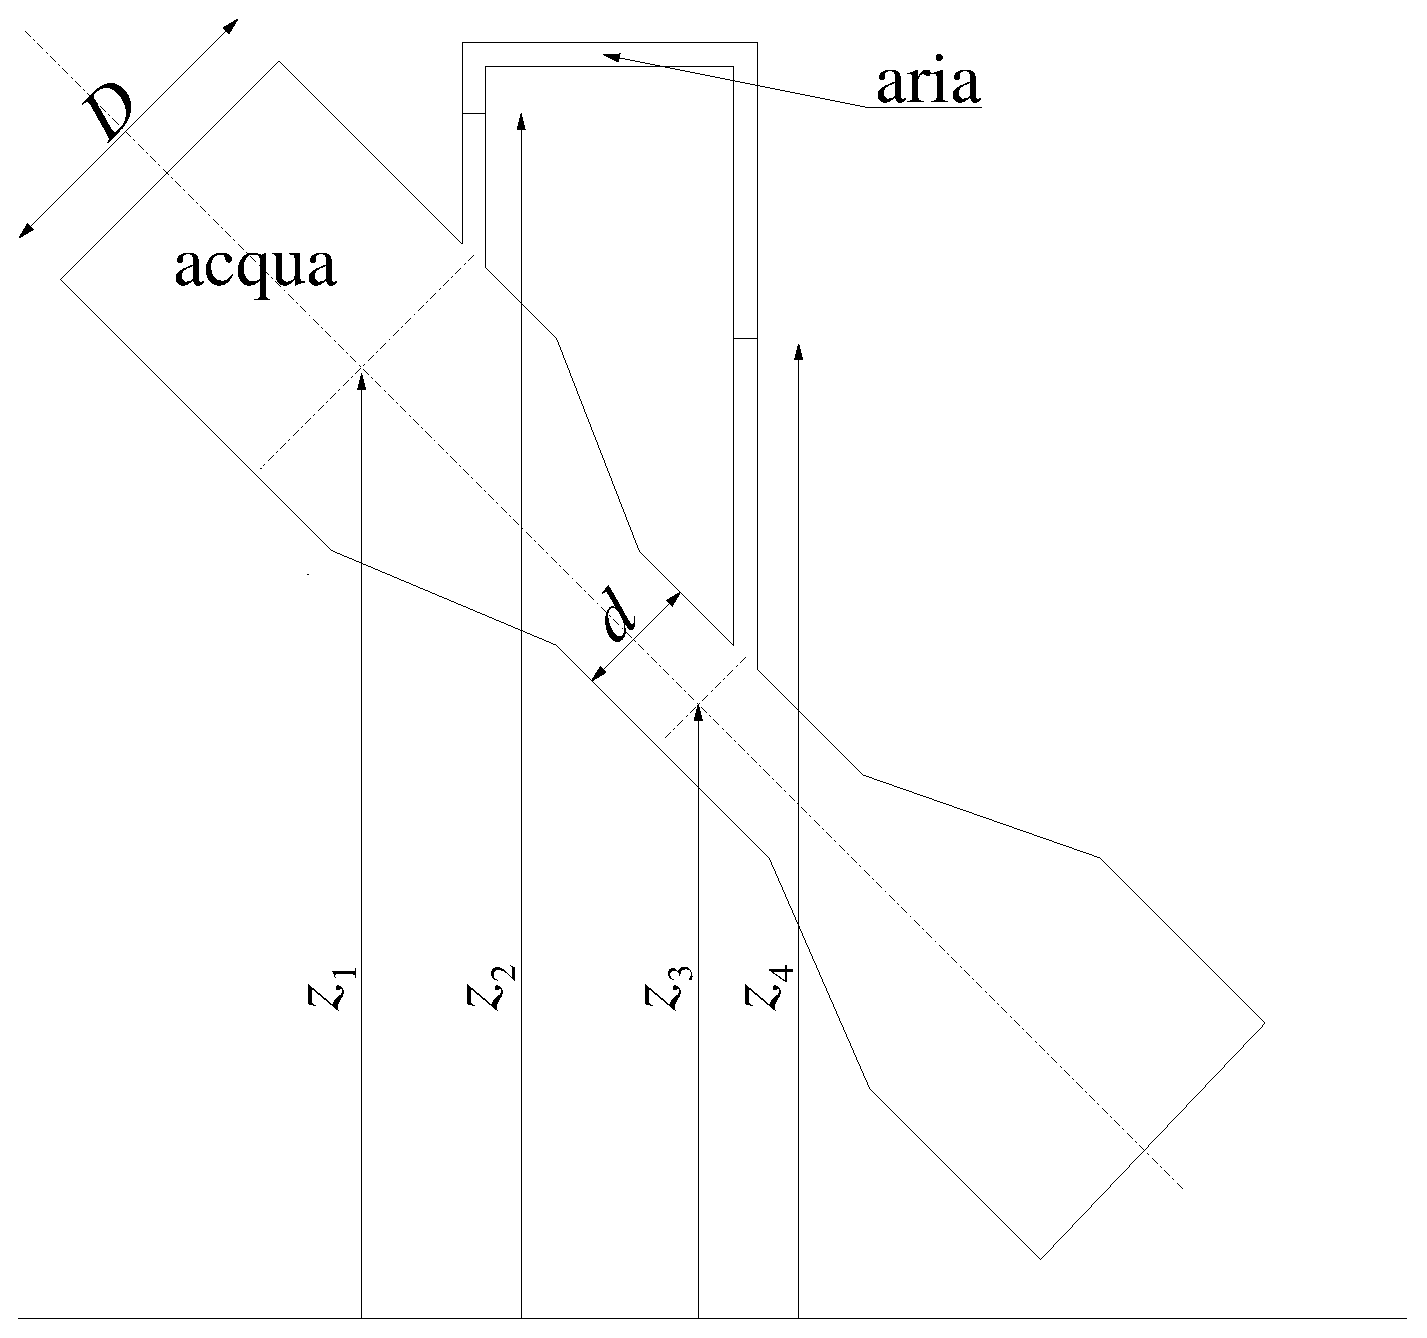
\includegraphics[width=0.90\textwidth]{./fig/venturi.eps}
   \end{center}
\end{minipage}
\end{tabular}

\sol

\partone
Teorema di Bernoulli. Equazione della vorticità. Conseguenze delle ipotesi di stazionarietà, fluido incomprimibile, non viscoso, irrotazionale. Dominio di applicabilità del teorema di Bernoulli. Condizioni all'interfaccia.
Legge di Stevino.

\parttwo
Il problema viene risolto in diversi passi successivi: in principio vengono fatte alcune ipotesi semplificative ($\rho = \bar{\rho}$, $\mu=0$, $\frac{\partial}{\partial t}=0$); poi si utilizza l'equazione della vorticità per semplificare ulteriormente il problema; si determina il dominio in cui è applicabile il teorema di Bernoulli con le ipotesi fatte; si osserva che la parte restante del problema è un problema di statica; si determinano le condizioni di interfaccia tra i due domini; solo a questo punto è possibile scrivere il sistema di equazioni dal quale ricavare le quantità richieste dal problema.

\begin{itemize}

\item 
Il testo del problema consente di fare le seguenti ipotesi: fluido incomprimibile, non viscoso, stazionario. 

\item
L'ipotesi di flusso non viscoso e quella di velocità uniforme a monte permettono di definire il domino all'interno del quale è possibile applicare il teorema di Bernoulli, aggiungendo l'ipotesi di irrotazionalità alle tre ipotesi precedenti. Infatti, l'equazione della vorticità può essere scritta come:
\begin{equation}
  \frac{D \bm{\omega}}{Dt} = (\bm{\omega} \cdot \bm{\nabla}) \bm{u}
\end{equation}
La derivata materiale rappresenta la variazione di una quantità associata a una particella materiale che segue il moto del fluido. Poiché la vorticità nella sezione a monte è nulla (il profilo di velocità è uniforme quindi le derivate spaziali sono nulle), la vorticità rimane nulla ($\frac{d f}{d t} = a f$, se $f=0$ all'istante iniziale la sua derivata in quell'istante è nulla, quindi $f$ non varia, quindi rimane uguale a zero).

\item
Il dominio in cui è possibile applicare il teorema di Bernoulli con le ipotesi di incomprimibilità, assenza di viscosità ed effetti dissipativi, stazionarietà, \textbf{irrotazionalità} e connessione semplice del dominio, coincide con il tubo di Venturi stesso. Infatti in corrispondenza delle prese a parete cade l'ipotesi di irrotazionalità.

Secondo le ipotesi fatte il fluido è non viscoso. Questo assicura che la vorticità sia nulla lungo le linee di corrente. Nel tubo del manometro però il fluido è fermo. Per un fluido non viscoso in corrispondenza dell'interfaccia non ci deve essere discontinuità nella componente normale all'interfaccia stessa e nella pressione. La componente normale è nulla da entrambe le parti della discontinuità; la componente tangenziale è però discontinua: mentre nel tubo di Venturi è diversa da zero, nel tubo del manometro è nulla. Questo comporta che la vorticità non sia nulla (bensì infinita: "differenza finita in uno spessore infinitesimo") e di conseguenza la non validità in questa regione delle ipotesi fatte in precedenza. 

Si possono quindi distinguere due regioni (il tubo di Venturi e il manometro) che non possono "parlare" tra di loro con il teorema di Bernoulli, ma solo tramite la condizione di \textbf{interfaccia} (continuità degli sforzi: per fluidi non viscosi questa condizione coincide con la continuità della pressione).

\begin{figure*}
\centering
\subfloat[][\emph "Suddivisione" del dominio: in tonalità rosse il dominio nel quale è lecito applicare le leggi della statica, in tonalità blu quello nel quale viene applicato il teorema di Bernoulli.]
   {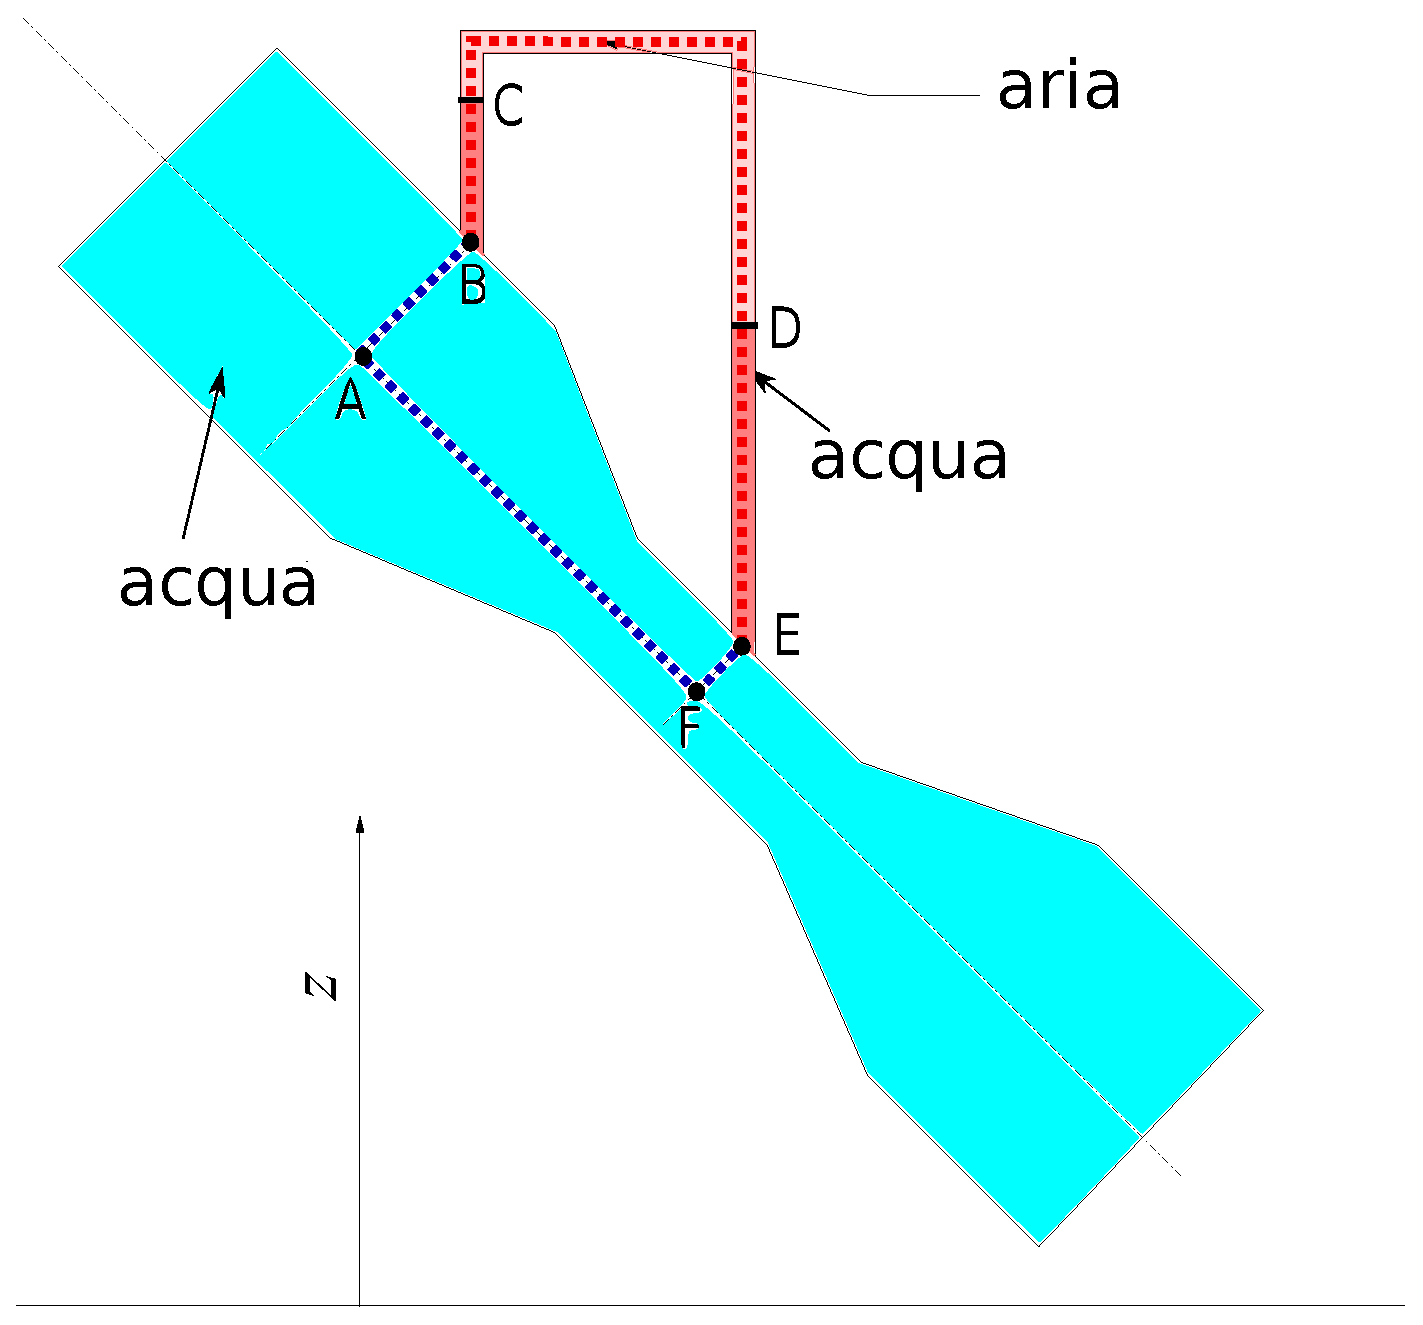
\includegraphics[width=.40\textwidth]{./fig/venturiDomain.eps}} \quad
\subfloat[][\emph Condizioni all'interfaccia. Superficie di discontinuità di velocità e vorticità infinita; la pressione invece è continua. I punti $B_1$ e $B_2$ identificano lo stesso punto al di qua e al di là dell'interfaccia.]
   {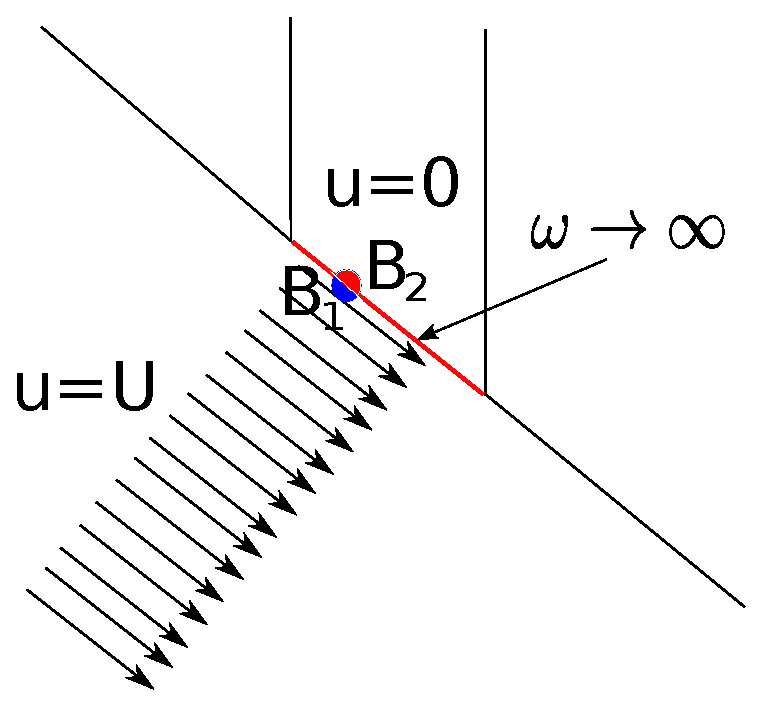
\includegraphics[width=.40\textwidth]{./fig/Discont.eps}}
\end{figure*}

\item \'E possibile ora scrivere il sistema risolvente:

\begin{equation}
\begin{cases}
 P_A + \frac{1}{2}U_A^2 + \rho g z_A = P_{B_1} + \frac{1}{2}U_{B_1}^2 + \rho g z_{B_1} & \text{(Bernoulli A-$B_1$)} \\
 P_{B_1} = P_{B_2} & \text{(interfaccia $B_1$-$B_2$)} \\
 P_{B_2} + \rho g z_{B_2} = P_C + \rho g z_C & \text{(Stevino $B_2$-C)} \\
 P_C + \rho_a g z_C = P_D + \rho_a g z_D & \text{(Stevino C-D)} \\
 P_D + \rho g z_D = P_{E_2} + \rho g z_{E_2} & \text{(Stevino D-$E_2$)} \\
 P_{E_2} = P_{E_1} & \text{(interfaccia $E_2$-$E_1$)} \\
 P_{E_1} + \frac{1}{2} \rho U_{E_1}^2 + \rho g z_{E_1} = P_F + \frac{1}{2} \rho U_F^2 + \rho g z_F & \text{(Bernoulli $E_1$-F)} \\
 P_A + \frac{1}{2}\rho U_A^2 + \rho g z_A = P_F + \frac{1}{2}\rho U_F^2 + \rho g z_F & \text{(Bernoulli A-F)} \\
 \rho \frac{\pi D^2}{4} U_A = \rho \frac{\pi d^2}{4} U_F & \text{(continuità A-F)}
\end{cases}
\end{equation}
che, osservando che $z_{B_1} = z_{B_2} = z_B$, $z_{E_1} = z_{E_2} = z_E$ e applicando le ipotesi fatte in precedenza ($U_A = u_{B_1}$, $U_F = u_{E_1}$, $P_{B_1} = P_{B_2} = P_B$, $P_{E_1} = P_{E_2} = P_E$), diventa:

\begin{equation}
\begin{cases}
 P_A + \rho g z_A = P_{B} + \rho g z_{B} & \text{(Bernoulli A-B)} \\
 P_{B_2} + \rho g z_{B} = P_C + \rho g z_C & \text{(Stevino B-C)} \\
 P_C + \rho_a g z_C = P_D + \rho_a g z_D & \text{(Stevino C-D)} \\
 P_D + \rho g z_D = P_{E} + \rho g z_{E} & \text{(Stevino D-E)} \\
 P_{E_1} + \rho g z_{E} = P_F +  + \rho g z_F & \text{(Bernoulli E-F)} \\
 P_A + \frac{1}{2} \rho U_A^2 + \rho g z_A = P_F + \frac{1}{2}\rho U_F^2 + \rho g z_F & \text{(Bernoulli A-F)} \\
 D^2 U_A = d^2 U_F & \text{(continuità A-F)}
\end{cases}
\end{equation}

Anche se il numero di equazioni è minori del numero di incognite, prova che il sistema è indeterminato, si dimostra che $U_A$ e $U_F$ sono determinate (nelle equazioni intervengono sempre differenze di pressioni, ed è questo il motivo dell'indeterminazione).

\item Soluzione del sistema: il sistema può essere risolto come più si preferisce. Per esempio, partendo da quella che può essere una "lettura dello strumento" $\Delta z = z_C - z_D$ e "chiudendo il ciclo ABCDEF":

\begin{equation}
  \rho_a g \Delta z = P_D - P_C
\end{equation}

\begin{equation}
  \begin{cases}
    P_D = P_E + \rho g (h_E - h_D) = P_F + \rho g (h_F - h_D)\\
    P_C = P_B + \rho g (h_B - h_C) = P_A + \rho g (h_A - h_C)\\
  \end{cases} \\
\end{equation}

\begin{equation}
\begin{aligned}
  \Rightarrow \quad P_D - P_C & = (P_F + \rho g h_F) - (P_A + \rho g h_A) + \rho g \Delta z = 
  & \text{(Bernoulli A-F)}\\
   & = \frac{1}{2}\rho U_A^2 - \frac{1}{2}\rho U_F^2 + \rho g \Delta z = 
  & \text{(continuità)}\\
   & = -\frac{1}{2}\rho U_A^2 \displaystyle\left( \frac{D^4}{d^4} - 1 \right) + \rho g \Delta z \\
\end{aligned}
\end{equation}

E quindi: 

\begin{equation}
  (\rho - \rho_a ) g \Delta z = \frac{1}{2}\rho U_A^2 \displaystyle\left( \frac{D^4}{d^4} - 1 \right)
\end{equation}

\begin{equation}
  U_A = \displaystyle\sqrt{\frac{2 (1 - \rho_a / \rho) g \Delta z}{\frac{D^4}{d^4} - 1}}
\end{equation}

Inserendo i valori numerici, si trova: $U = 0.956 m/s$, $Q = 3.0 \cdot 10^{-4} m^3/s$, $\bar{Q} = 3.0 \cdot 10^{-1} kg/s$.

\end{itemize}


\textit{Osservazioni.} \'E importante saper riconoscere i limiti di applicabilità di formule e teoremi nel rispetto delle ipotesi con le quali essi vengono formulati.

Considerazioni analoghe dovranno essere svolte anche in esercizi simili a questo, riguardanti le soluzioni esatte delle equazioni di Navier-Stokes.

\newpage
\noindent
\begin{tabular}{cc}
\begin{minipage}[b]{0.60\textwidth}
\begin{exerciseS}[Efflusso da serbatoio]
Si consideri il serbatoio rappresentato in figura, $D=2\ m$, 
$H=4.4\ m$ al cui interno \`{e} contenuta acqua, 
$\overline{\rho}=999\,{kg/m^3}$. 
Supponendo il fluido non viscoso, determinare la velocit\`{a} di 
efflusso del fluido dall'ugello del serbatoio, $h=0.4\ m$ 
e $d = 1\ cm$, e la sua portata, sia in massa sia in volume.

($U = 8.86\ m/s$, $Q=6.96\, 10^{-4}\ m^3/s$, $\overline{Q}=0.695\ kg/s$)
\end{exerciseS}
\end{minipage}
&
\begin{minipage}{0.35\textwidth}
   \begin{center}
   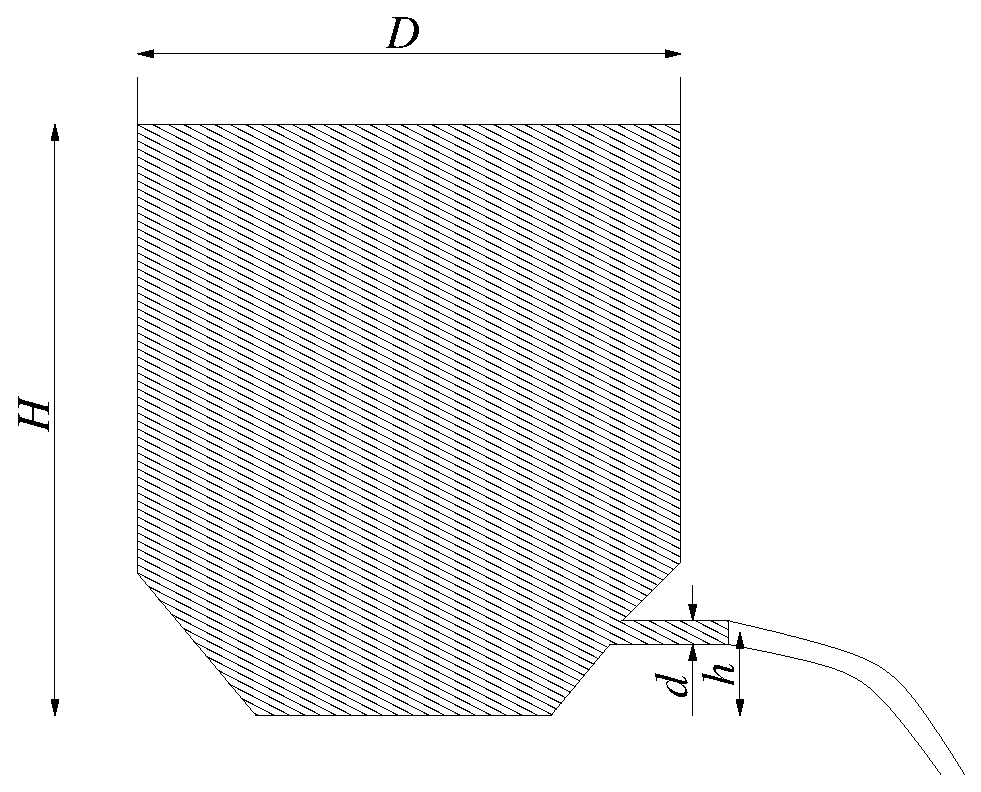
\includegraphics[width=0.90\textwidth]{./fig/serbatoio.eps}
   \end{center}
\end{minipage}
\end{tabular}

\sol

\partone
 Teorema di Bernoulli, nel caso incomprimibile, non viscoso, "stazionario" (da come è
 fatto il disegno, il livello del serbatorio sembra diminuire...assumiamo che così non sia), con forze che ammettono
potenziale e dominio semplicemente connesso.
Se si fa l'ipotesi che il flusso sia irrotazionale sulla sezione di ingresso, nel caso non viscoso, 
si mantiene irrotazionale ovunque (equazione della vorticità).
\begin{equation}
  \frac{D \bm{\omega}}{Dt} = (\bm{\omega} \cdot \bm{\nabla}) \bm{u}
\end{equation}

Si può quindi scrivere il teorema di Bernoulli nella forma:
\begin{equation}
  \frac{P}{\rho} + \frac{|\bm{u}|^2}{2} + gh = \text{cost}
\end{equation}

\parttwo
 Il problema si risolve mettendo a sistema il teorema di Bernoulli (opportunamente
semplificato; vedi sopra) con il bilancio integrale di massa. Si ipotizza che sulle due sezioni agisca la stessa pressione esterna.

\begin{equation}
\begin{cases}
  A_1 u_1 = A_2 u_2 & (massa) \\
  \frac{u_1^2}{2} + g h_1 = \frac{u_2^2}{2} + g h_2 & (Bernoulli)
\end{cases}
\end{equation}

Svolgendo i passaggi, ricordando che le superfici sono circolari, risulta:
\begin{equation}
  u_2 = \sqrt{\frac{2 g (h_1-h_2)}{1-\displaystyle\left(\frac{d_2}{d_1}\right)^4}}
\end{equation}

Si calcolano poi le portate volumetriche e di massa.
\begin{equation}
\begin{aligned}
  & Q = A_2 u_2 \\
  & \dot{m} = \rho Q
\end{aligned}
\end{equation}

\newpage
\noindent
\begin{tabular}{cc}
\begin{minipage}[b]{0.60\textwidth}
\begin{exerciseS}[Corrente in canale aperto]
Si consideri il flusso d'acqua, $\overline{\rho}=999\ kg/m^3$, 
nel canale rappresentato in figura.
Nel primo tratto l'acqua scorre con una velocit\`{a} uniforme 
$U_1 = 1\ m/s$  e l'altezza del pelo libero rispetto al fondo 
del canale \`e $h_1 = 1.5\ m$. Determinare la velocit\`{a}
dell'acqua $U_2$ e l'altezza del pelo libero $h_2$ nel secondo tratto 
del canale, sapendo che l'altezza del fondo del primo tratto rispetto al fondo
del secondo tratto \`{e} $H=0.5\ m$. Si trascuri qualunque effetto
dissipativo.

(Soluzione 1: $U_2 = 0.741\ m/s$, $h_2 = 2.022\ m$.
Soluzione 2: $U_2 = 5.940\ m/s$, $h_2 = 0.252\ m$)
\end{exerciseS}
\end{minipage}
&
\begin{minipage}{0.35\textwidth}
   \begin{center}
   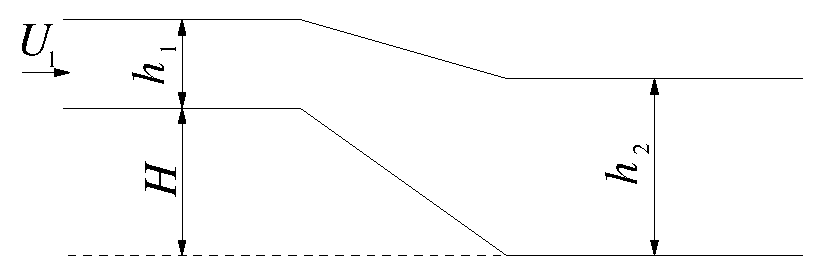
\includegraphics[width=0.90\textwidth]{./fig/canale.eps}
   \end{center}
\end{minipage}
\end{tabular}

\sol

\partone
Teorema di Bernoulli nel caso incomprimibile, non viscoso, stazionario, irrotazionale.
Soluzione di equazioni di terzo grado: metodo grafico e numerico. 
Correnti in canali aperti: soluzioni ``fisiche'', numero di Froude $Fr$,
 correnti subrcritiche e supercritiche.

\parttwo

L'esercizio viene risolto in due passi, che richiedono diversi livelli di
 conoscenza della dinamica dei fluidi in canali aperti: in un primo tempo,
 vengono ricavate le soluzioni ammissibili ($h_2 > 0$, $U_2 > 0$) del 
 problema; in un secondo tempo, viene scelta la soluzione fisica del
 problema, tra le due soluzioni ammissibili trovate in precedenza.

\paragraph{Parte 1.}
L'esercizio viene risolto mettendo a sistema il teorema di Bernoulli riferito
 a una linea di corrente sul pelo libero
(sul quale agisce la pressione ambiente $P_a$, costante) e l'equazione di
 continuità.
Grazie alle ipotesi elencate in precedenza, si può scrivere il sistema risolvente come:

\begin{equation}\label{eqn:bern_cont}
  \begin{cases}
    \frac{1}{2}\rho U_1^2 + \rho g(h_1+H) = \frac{1}{2}\rho U_2^2 +
    \rho g h_2 \\
    h_1 U_1 = h_2 U_2
  \end{cases}
\end{equation}

Il sistema è di due equazioni (non lineari) nelle incognite $U_2$ e $h_2$. Se si ricava una delle due incognite
da un'equazione e la si inserisce nell'altra, si ottiene un'equazione di terzo grado. Per esempio, ricavando $h_2$ 
dalla prima e inserendola nella seconda, per l'incognita $U_2$ si ottiene l'equazione di terzo grado:

\begin{equation}
  h_1 U_1 = U_2 \displaystyle\left( \frac{U_1^2 - U_2^2}{2 g} + (h_1 + H)    \right)
\end{equation}


I metodi numerici convergono (quando convergono) a una soluzione, senza informazioni su quante soluzioni
esistono effettivamente: prima di risolvere l'equazione di terzo grado con un
 metodo numerico è utile un primo approccio analitico al problema. 

Per questo cerchiamo le soluzioni del sistema di due equazioni per via grafica. Le equazioni del sistema \ref{eqn:bern_cont}
 definiscono curve nel piano $(U_2,h_2)$. Se scegliamo di usare come asse orizzontale quello delle $U_2$, la prima equazione definisce una parabola con la concavità diretta verso il basso ($h_2 = - 0.5  U_2^2 /g +...$), mentre la seconda un'iperbole.
 
\begin{center}
\begin{tikzpicture}[scale=0.80]
\begin{axis}[axis lines=middle, domain=-8.0:8.0, xlabel={$U_2$}, ylabel={$h_2$}]
\addplot
[domain=-8:8,samples=40,smooth,thick,blue]
{-0.5/9.81 * x^2 + 2.05};
\addplot
[domain=-8:-0.75,samples=40,smooth,thick,red]
{1.5/x};
\addplot
[domain=0.5:8,samples=40,smooth,thick,red]
{1.5/x};
\addplot[color=black,mark=x] coordinates{
         (0.741, 2.022)};
\addplot[color=black,mark=x] coordinates{         
         (5.940, 0.252)};
%\legend{$f_1(x)$,$\frac{\rho_s}{\rho}=0.842$}
\end{axis}
\end{tikzpicture}
\end{center}

Esistono due soluzioni con senso fisico ($h_2 \ge 0, U_2 \ge 0$). Ora che sappiamo quante soluzioni cercare e dove cercarle, possiamo procedere con un metodo numerico, dando guess iniziali in un intorno della soluzione.
Le due soluzioni sono:
\begin{equation}
\begin{aligned}
  A :
  \begin{cases}
   U_2 = 0.741 \ m/s \\
   h_2 = 2.022 \ m
  \end{cases}
   \quad
  B :
  \begin{cases}
   U_2 = 5.940 \ m/s \\
   h_2 = 0.252 \ m
  \end{cases}
\end{aligned}
\end{equation}

\paragraph{Parte 2.}
\'E plausibile farsi una domanda: al netto delle ipotesi fatte sul regime di
 moto (fluido incomprimibile, non viscoso), il modello è in grado di
 descrivere il fenomeno fisico e stabilire quale delle due soluzioni 
 amissibili trovate è la soluzione ``fisica''?
Seguendo la trattazione del problema svolta in \href{http://heidarpour.iut.ac.ir/sites/heidarpour.iut.ac.ir/files//u32/open-chaudhry.pdf}{Chaudhry, \textit{Open-Channel Flow}, paragrafo 2-7: Channel transition e paragrafi vicini},
 è possibile trovare l'unica soluzione fisica del problema.
 Viene introdotta la notazione usata da Chaudhry, che contrasta in parte
 con quella usata finora. Si tornerà alla notazione usata nella prima parte
 dell'esercizio, solo alla fine per scrivere i risultati.

La variabile
 $z(x)$ descrive la quota del fondo del canale, la variabile $y(x)$ descrive
 la profondità della corrente, riferita al fondo del canale. Si indica
 con $Q = V y $ la portata in volume, costante.
Il trinomio di Bernoulli $H$, diviso per $\rho$ e $g$, è costante lungo il
 canale. Si ricorda che sulla linea di corrente in corrispondenza del pelo
 libero agisce una pressione costante uguale alla pressione ambiente $P_a$.
Se si introduce la coordinata orizzontale $x$,
\begin{equation}
\begin{aligned}
 0 = \dfrac{d H}{d x} = 
 & \dfrac{d (y+z)}{d x} + \dfrac{d}{d x} \dfrac{V^2}{2 g}     = \\
 & = \dfrac{d (y+z)}{d x} + \dfrac{d}{d x} \dfrac{Q^2}{2 g y^2} = \\
 & = \dfrac{d (y+z)}{d x} - \dfrac{Q^2}{g y^3} \dfrac{d y}{d x} = \\
 & = \dfrac{d (y+z)}{d x} - \dfrac{V^2}{g y} \dfrac{d y}{d x} = \\ 
 & = \dfrac{d (y+z)}{d x} - \text{Fr}^2 \dfrac{d y}{d x} = \\ 
 & = \dfrac{d z}{d x} - (\text{Fr}^2 - 1) \dfrac{d y}{d x} \\ 
\end{aligned}
\end{equation}
dove è stato introdotto il numero di Froude $\textit{Fr} = V(y)^2 / g y$, e
 qui è stata esplicitata la dipendenza dalla profondità $y$, funzione a sua
 volta funzione della coordinata $x$.
Si trova così il legame tra la profondità della corrente $y(x)$, la quota
 del fondo $z(x)$ e lo stato della corrente, descritto dal numero di Froude.
\begin{equation}\label{eqn:flow_depth}
 \dfrac{d z}{d x} = (\text{Fr}^2(y(x)) - 1) \dfrac{d y}{d x}
\end{equation}
Vengono definiti due regimi di moto: subcritico $\textit{Fr} < 1$,
 supercritico $\textit{Fr} > 1$. Il profilo del fondo $z(x)$,
 e quindi la sua derivata, è noto dal progetto del canale.
 La profondità della corrente $y(x)$ può essere ottenuta integrando l'eq.
 \ref{eqn:flow_depth} con le condizioni iniziali note sulla sezione di 
 ingresso.

Per risolvere il nostro esercizio è sufficiente ragionare sui segni dei tre
 termini dell'eq. \ref{eqn:flow_depth}: $dz/dx \le 0$, quindi i due fattori
 alla destra dell'uguale devono essere discordi.
Il numero di Froude sulla sezione di ingresso del problema vale
 $\text{Fr}_1 = U^2_1 / (g h_1) = 0.068$, quindi il contenuto della parentesi
 tonda è negativo (e negativo rimane, al variare di $x$; di questo dovete
 fidarvi...).
 Deve quindi essere $dy/dx \ge 0$. Tornando alla notazione usata nella prima
 parte dell'esercizio, dove la profondità della corrente è indicata con
 $h(x)$, $dh(x)/dx \ge 0$. Poichè la profondità della corrente aumenta
 sempre, la soluzione ``fisica'' tra le due ammissibili è la soluzione $A$,
 per la quale $h_2 > h_1$.

\begin{equation}
  \begin{cases}
   U_2 = 0.741 \ m/s \\
   h_2 = 2.022 \ m
  \end{cases}
\end{equation}

\vspace{0.5cm}
\paragraph{Cosa non è stato detto.} \'E stato fatto solo un accenno al 
 ragionamento che consente di determinare l'unica soluzione ``fisica'' del
 problema delle correnti in canali aperti che variano con continuità.
 Non si dirà nulla sui salti idraulici (che portano la corrente da uno
 stato supercritico a uno subcritico), dei quali si possono trovare 
 esempi nei fiumi o sul fondo di un lavandino.
Si accenna solo alla uguaglianza formale del problema del moto
 di un fluido incomprimibile in un canale aperto, con il moto
 monodimensionale di un 
 fluido comprimibile, dove il ruolo del numero di Froude $\textit{Fr}$
 sarà svolto dal numero di Mach $M$, la definizione di stato sub- e
 supercritico, sarà sostituita da quella di condizione sub- e supersonica,
 il salto idraulico troverà il suo fenomeno corrispondente nelle onde d'urto.

\newpage
\noindent
\begin{tabular}{cc}
\begin{minipage}[b]{0.60\textwidth}
\begin{exerciseS}[Tubo di Pitot statico]
Dato il condotto a sezione circolare rappresentato in figura, 
determinare la portata in massa d'olio, $\overline{\rho} = 850\ kg/m^3$,
attraverso il condotto stesso sapendo che il diametro del condotto 
\`{e} $d=0.5\ m$, che la differenza di altezza fra i peli liberi 
\`{e} $H=40\ cm$, che il diametro del tubo ``a U'' \`{e} di $2$ mm. 
Si trascuri qualunque effetto dissipativo, si assuma
uniforme la velocit\`{a} in una sezione sufficientemente lontana a monte
e si consideri che nel tubo ``a U'' sia presente aria in condizioni normali.

($\overline{Q}= 467.2\  kg/s$)
\end{exerciseS}
\end{minipage}
&
\begin{minipage}{0.35\textwidth}
   \begin{center}
   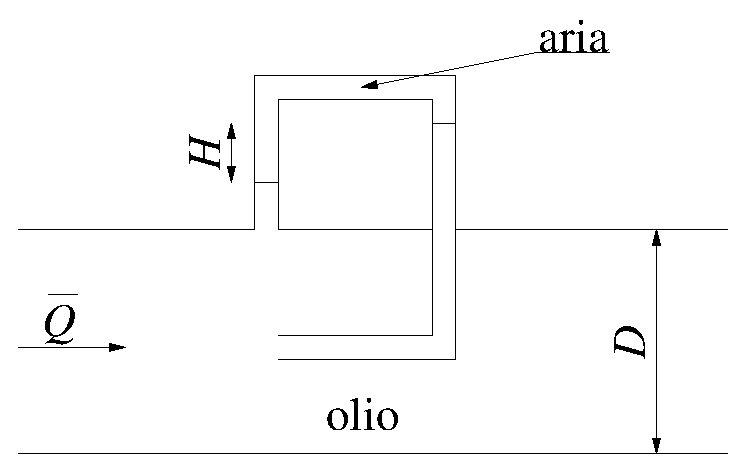
\includegraphics[width=0.90\textwidth]{./fig/condottocircolare.eps}
   \end{center}
\end{minipage}
\end{tabular}

\sol

\partone
 Teorema di Bernoulli nell'ipotesi di stazionarietà, fluido incomprimibile, non viscoso, irrotazionale.
Equazione della vorticità nel caso non viscoso.
Legge di Stevino.

\parttwo
Vengono fatte alcune ipotesi semplificative ($\rho = \bar{\rho}$, $\mu=0$, $\frac{\partial}{\partial t}=0$); si utilizza poi l'equazione della vorticità per semplificare ulteriormente il problema: se si assume che il profilo di velocità all'ingresso sia uniforme, e quindi a vorticità nulla, il fluido nel canale rimane irrotazionale (dall'equazione della vorticità per fluidi non viscosi).

Gli unici due punti che possono creare problemi sono i collegamenti del tubo con il canale.
Sulla linea di corrente che incontra l'imbocco del tubicino, il fluido subisce un rallentamento dalla velocità di ingresso fino ad arrestarsi: su questa linea di corrente è possibile applicare il teorema di Bernoulli.
In corrispondenza del'altro collegamento, si incontra una superficie di discontinuità a vorticità infinita: non è quindi possibile attraversare questa superficie applicando direttamente il teorema di Bernoulli, ma bisogna ricorrere alle condizioni di interfaccia tra i due domini, quello interno al canale e quello interno al tubo, nel quale possono essere applicate le equazioni della statica.

Vengono definiti i punti  $A$  all'ingresso sulla linea di corrente che arriva alla presa del tubo all'interno del canale; il punto $B$ coincidente con la presa del tubo all'interno del canale; $C$ il pelo libero di destra all'interno del tubo ``a U'', $D$ il pelo libero di sinistra. Si definiscono anche $h_C$ e $h_D$ come quote dei peli liberi (oss. $H = h_C - h_D$).

\begin{center}
  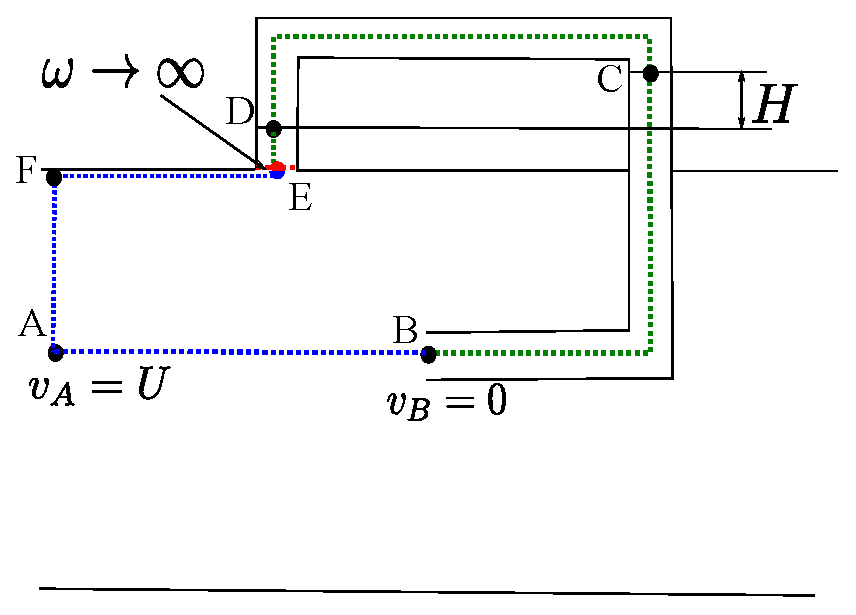
\includegraphics[width=0.35\textwidth]{./fig/Canale01.eps}
\end{center}

Il sistema risolvente è:
\begin{equation}
\begin{cases}
  P_A + \frac{1}{2} \rho v_A^2 + \rho g h_A =
   P_B + \frac{1}{2} \rho v_B^2 + \rho g h_B\\
  P_B + \rho g h_B = P_C + \rho g h_C   \\
  P_C + \rho_a g h_C = P_D + \rho_a g h_D\\
  P_D + \rho g h_D = P_{E_2} + \rho g h_{E_2} \\
  P_{E_2} = P_{E_1} \\
  P_{E_1} + \frac{1}{2} \rho u_{E_1}^2 + \rho g h_{E_1} = P_F + \frac{1}{2} \rho u_F^2 + \rho g h_F\\
 P_F + \frac{1}{2} \rho v_F^2 + \rho g h_F = P_A + \frac{1}{2} \rho v_A^2 + \rho g h_A \\
  \bar{Q} = \rho \frac{\pi}{4}d^2 U
\end{cases}
\end{equation}

Osservando che $h_A = h_B$, $h_E = h_F$, $v_A = v_F = U$, 
$v_B = 0$, supponendo $u_E = U$ (ipotizzando dimensioni e intrusività trascurabile della sonda), il sistema semplificato diventa:
\begin{equation}
\begin{cases}
  P_A + \frac{1}{2} \rho U^2  = P_B \\
  P_B + \rho g h_A = P_C + \rho g h_C   \\
  P_C + \rho_a g h_C = P_D + \rho_a g h_D\\
  P_D + \rho g h_D = P_E + \rho g h_E \\
  P_E + \frac{1}{2} \rho u_E^2 = P_F + \frac{1}{2} \rho U^2 \\
 P_F + \rho g h_E = P_A + \rho g h_A \\
  \bar{Q} = \rho \frac{\pi}{4}d^2 U
\end{cases}
\end{equation}

Risolvendo per U, avendo definito $H = h_C - h_D$:
\begin{equation}
  \frac{1}{2} \rho U^2 = P_B - P_A = ... = (\rho - \rho_a) g H \quad \Rightarrow \quad 
  U = \sqrt{2\displaystyle\left(1-\frac{\rho_a}{\rho}\right) g H}
\end{equation}

Inserendo i valori numerici: $U = 2.799 m/s$, $\bar{Q} = 467.15 kg/s$.



\newpage
%\input{./capitoli/05_bernoulli/0505in}
%\newpage
\noindent
\begin{tabular}{cc}
\begin{minipage}{0.60\textwidth}
\begin{exerciseS}[Getto libero]
Si consideri un getto stazionario, assialsimmetrico, d'acqua in 
condizioni standard, diretto verso l'alto, in atmosfera uniforme, 
secondo la verticale $z$, e uscente con velocit\`{a} uniforme e 
costante $V = 20\ m/s$ da un ugello circolare di diametro 
$d = 5\  cm$. Si assuma che:
\begin{itemize}
\item la curvatura delle linee di flusso sia trascurabile;
\item sia trascurabile ogni perdita di energia.
\end{itemize}
Si determinino:
\begin{itemize}
\item[a)] il diametro $D$ del getto alla quota $Z = 15\ m$
          (misurata dal piano d'uscita dall'ugello);
\item[b)] la massima quota ideale $H$ cui pu\`{o} giungere il getto.
\end{itemize}
($D = 6.97\ cm$, $H = 20.39\  m$)
\end{exerciseS}
\end{minipage}
&
\begin{minipage}{0.35\textwidth}
   \begin{center}
   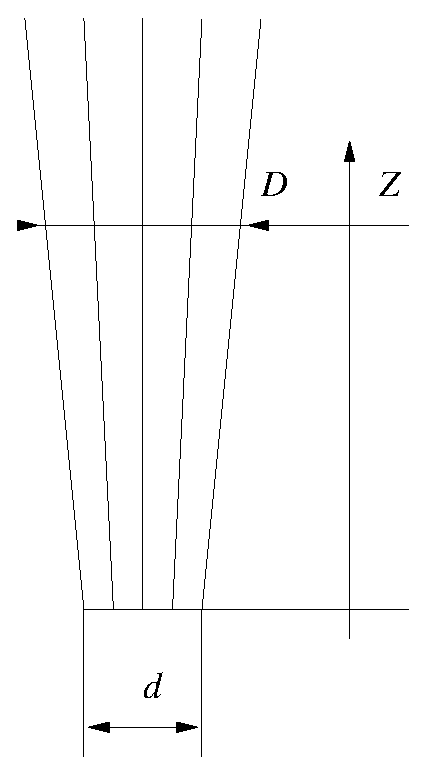
\includegraphics[width=0.60\textwidth]{./fig/getto_vert.eps}
   \end{center}
\end{minipage}
\end{tabular}

\sol

\partone
 Teorema di Bernoulli nell'ipotesi di stazionarietà, fluido incomprimibile, non viscoso, irrotazionale.
Equazione della vorticità nel caso non viscoso.

\parttwo

\begin{itemize}
\item Il primo quesito del problema viene risolto mettendo a sistema l'equazione di
 Bernoulli (ipotesi...) e l'equazione della continuità.
\begin{equation}
\begin{cases}
  \frac{1}{2} \rho V^2  = \frac{1}{2}\rho u^2(z) + \rho g z\\
  V d^2 = u(z) D^2
\end{cases} \qquad \Rightarrow \qquad D = \frac{d}
{\displaystyle\left[1 - \frac{2 g z}{V^2}\right]^{\frac{1}{4}}}
\end{equation}
 Inserendo i valori numerici $D = 6.97 \text{cm}$.

\item Il secondo quesito si ottiene ricavando dal teorema di Bernoulli la quota alla quale 
la velocità è nulla.

\begin{equation}
  \frac{1}{2} \rho V^2 = \rho g H \qquad \Rightarrow \qquad 
  H = \frac{1}{2} \frac{V^2}{g}
\end{equation}
 Inserendo i valori numerici $H = 20.39 \text{m}$.

\end{itemize}



\newpage
\begin{minipage}[l]{0.5\textwidth}
 \begin{exerciseS}[Giochi d'acqua]
  In un gioco d'acqua ($\rho=999\ kg/m^3$), un disco di diametro $D=35\ cm$ viene sollevato 
  da un getto che fuoriesce con velocit\`{a} $V_0=10\ m/s$ da un foro di diametro $d_0=8\ cm$ concentrico 
  all'asse del disco, cos\`i come illustrato schematicamente in figura. Noto che in condizioni 
  stazionarie la quota raggiunta dal disco \`{e} di poco superiore alla quota $H=2\ m$, si richiede 
  di determinare:
  \begin{itemize}
   \item[1.1)] la velocità $V_1$ e il diametro $d_1$ del getto alla quota $H$
         supponendo trascurabili tra le sezioni $0$ e $1$ sia la curvatura delle linee di flusso 
         che ogni forma di dissipazione;
   \item[1.2)] lo spessore $h$ del film d'acqua all'estremit\`{a} del disco assumendo
         che il profilo di velocit\`{a} radiale sia lineare con velocit\`{a} massima $V_2=V_1$.     
   \item[1.3)] la massa $m$ del disco considerando trascurabili sia gli sforzi viscosi all'interfaccia tra l'atmosfera 
               circostante ($P_{atm}=101325\ Pa$) e il getto d'acqua che la forza gravitazionale agente sul fluido 
               tra la quota $H$ e la quota del disco.
  \end{itemize}
 \end{exerciseS}
 \textit{Per la risoluzione del problema si assumano condizioni di assialsimmetria.}
\end{minipage}
\hspace{3mm}
\begin{minipage}[r]{0.5\textwidth}
 \centering
  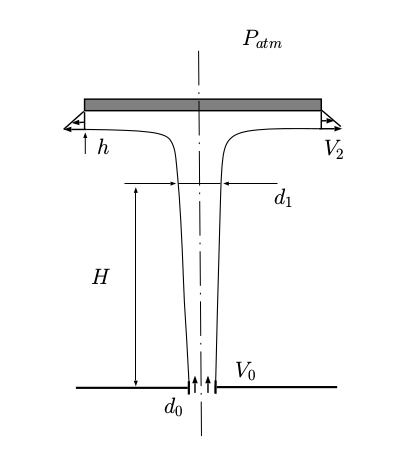
\includegraphics[width=1.0\textwidth]{./fig/jet}
\end{minipage}

\sol

\partone
 Teorema di Bernoulli nell'ipotesi di stazionarietà, fluido incomprimibile, non viscoso, irrotazionale. Bilanci integrali.
 
\parttwo
\begin{itemize}

\item Il primo punto viene risolto mettendo a sistema il teorema di Bernoulli e la 
continuità.
\begin{equation}
\begin{cases}
  \frac{1}{2} \rho V_0^2  = \frac{1}{2}\rho V_1^2(z) + \rho g H\\
  V_0 d_0^2 = V_1 d_1^2
\end{cases} \qquad \Rightarrow \qquad 
\begin{cases}
  V_1 = V_0\sqrt{1 - 2 g H / V_0^2} \\
  d_1 = \displaystyle\left[1 - \frac{2 g H}{V_0^2}\right]^{-\frac{1}{4}} d_0
\end{cases}
\end{equation}

\item Il secondo punto viene risolto utilizzando solamente il bilancio di massa.
\begin{equation}
  Q = \frac{\pi}{4} \rho V_0 d_0^2 = \frac{\pi}{4} \rho V_1 d_1^2 = \frac{\pi}{2} D h V_2 \qquad \Rightarrow \qquad h = \frac{d_1^2}{2 D}
\end{equation}

\item Il terzo punto viene risolto applicando il bilancio della quantità di moto in
direzione verticale per trovare la forza applicata dal disco al fluido. Infine si 
scrive l'equilibrio del disco soggetto alla stessa forza con verso opposto (principio
di azione e reazione) e al proprio peso.

Dal bilancio si ottiene che la componente verticale della forza che si scambiano fluido e disco è uguale a $\rho V_1^2 \frac{\pi}{4} d_1^2$. La massa del disco è quindi $m = \frac{\pi}{4} d_1^2 \frac{\rho V_1^2}{g}$

\end{itemize}






\newpage
\begin{minipage}[l]{0.5\textwidth}
  \begin{exerciseS}[Lamina inclinata]
 Un getto di acqua ($\rho = 1000 \ kg/m^3$) colpisce una lamina
 di massa per unità di apertura $m = 1 \ kg/m$ inclinata di un 
 angolo $\alpha = 30\degree$ rispetto all'orizzontale, connessa a terra
 con una molla di costante elastica $k = 10^5 \ N/m^2$. 
 Il getto esce con profilo uniforme $U=10 \ m/s$ da una fessura
 larga $d_1 = 5 \ cm$
 Determinare:
 \begin{itemize}
   \item la velocità $U_2$ (uniforme) e lo spessore $d_2$ del getto
     alla quota $H=1 \ m$ sopra la fessura di uscita, supponendo 
     trascurabili ogni forma di dissipazione e la curvatura delle 
     linee di corrente;
   \item la velocità massima $V$ del profilo triangolare di spessore
     $h = 2 \ cm$, identico su entrambe le estremità della lamina;
   \item la deformazione della molla, considerando trascurabili gli 
     sforzi viscosi all'interfaccia tra il getto e l'atmosfera 
     circostante ($P_a = 101325 \ Pa$) e la
     gravità agente sul fluido al di sopra della quota $H$.
 \end{itemize}
 \end{exerciseS}

\end{minipage}
\hspace{3mm}
\begin{minipage}[r]{0.5\textwidth}
 \centering
  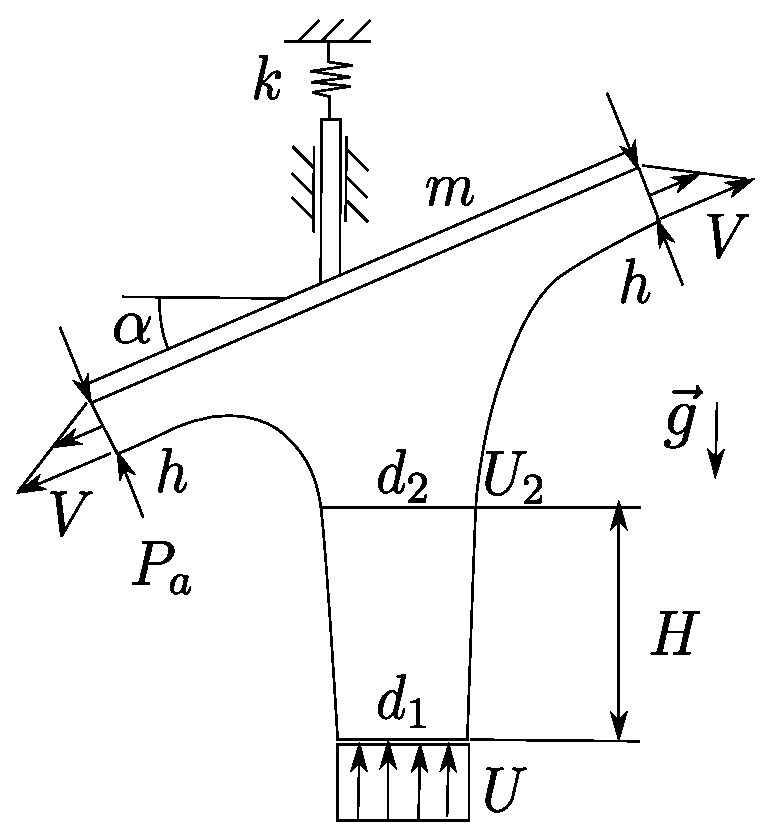
\includegraphics[width=1.0\textwidth]{./fig/jet_angle}
\end{minipage}

\sol

\partone
 Teorema di Bernoulli nell'ipotesi di stazionarietà, fluido incomprimibile, non viscoso, irrotazionale. Bilanci integrali.
 
\parttwo
\begin{itemize}
  \item continuità + Bernoulli
    \begin{equation}
      \begin{cases}
        \rho d U = \rho d_2 U_2 \\
        \frac{1}{2} \rho U^2 = \frac{1}{2} \rho U_2^2 + \rho g H
      \end{cases}
      \qquad \Rightarrow \qquad
      \begin{cases}
        d_2 = d_1 \left( 1 - \dfrac{2 g H}{U^2} \right)^{-1/2} = 0.0558 \ m \\
        U_2 = U \left( 1 - \dfrac{2 g H}{U^2} \right)^{1/2} = 8.96 \ m/s \\
      \end{cases}
    \end{equation}
  \item continuità: in ingresso profilo uniforme, in uscita due profili triangolari.
    \begin{equation}
      U d_1 = 2 \dfrac{1}{2} V h \Rightarrow V = U \dfrac{d_1}{h} = 25 \ m/s
    \end{equation}
  \item  bilancio di massa + equilibrio corpo: pressione $P_a$ ovunque; 
  i due flussi di quantità di moto sulla lamina si bilanciano: rimane 
  solo il termine in ingresso  
    \begin{equation}
    \bm{R}_{fl} = - \oint_{\partial \Omega} \rho \bm{u} \bm{u}
    \cdot \bm{\hat{n}}  =  \dots  = \rho U^2 \dfrac{d_1^2}{d_2} \bm{\hat{y}} = 4482.7 \ N \bm{\hat{y}}
    \end{equation}
    \begin{equation}
      k \Delta x = m g - R \Rightarrow \Delta x = - 0.0447 \ m \ \text{(compressione)}
    \end{equation}
\end{itemize}






\newpage

\cleardoublepage

% 06. soluzioni esatte -----------------
\chapterimage{blank_fig}
\chapter{Soluzioni esatte}\index{Soluzioni esatte}\label{ch:slnEsatte}

\section{Introduzione e linee guida per la soluzione dei problemi}

%Vengono fornite delle linee guida per risolvere i problemi sulle soluzioni esatte delle equazioni di Navier-Stokes.
\'E possibile ricavare alcune soluzioni esatte stazionarie delle equazioni di Navier-Stokes, che descrivono il moto di un fluido viscoso, quando il dominio ha una geometria ``semplice''. In alcuni casi, come la corrente in un canale piano (Newton-Couette), la corrente in un tubo a sezione circolare (Poiseuille), o la corrente nel setto tra due cilindri rotanti (Taylor-Couette), per semplificare le equazioni è possibile sfruttare l'omogeneità del dominio (in qualche direzione) e, per ipotesi, della corrente. Nella maggioranza delle soluzioni esatte, i termini non lineari nelle equazioni si annullano, permettendo di ricavare abbastanza facilmente la soluzione delle equazioni.

In generale, le soluzioni stazionarie esatte presentate in questo capitolo sono significative quando il regime di moto è laminare. Senza entrare molto nel dettaglio, una soluzione stazionaria è una soluzione di equilibrio delle equazioni di Navier-Stokes, per la quale $\partial \bm{u}/\partial t = \bm{0}$. Un regime di moto instazionario può manifestarsi a causa di una ``instabilità intrinseca'' della corrente o a causa di una enorme amplificazione (\textit{ricettività}) di disturbi, anche di intensità minima, sempre presenti in natura\footnote{
Il regime di moto periodico (e ordinato) che si manifesta nella corrente attorno a un cilindro quando il numero di Reynolds supera un valore critico ($Re_c \approx 46$) è il risultato di una ``instabilità intrinseca'' (\textit{globale}) parametrica del sistema. La soluzione stazionaria stabile esistente per $Re < Re_c$ diventa instabile quando il parametro $Re$ eccede il valore critico e nasce un ciclo limite (stabile) nel piano delle fasi del sistema. Il moto periodico e ordinato del sistema osservato nello sviluppo della \textit{scia di Von Karman} a valle del cilindro, corrisponde alla dinamica del sistema sul ciclo limite.
\newline
Mentre la corrente attorno a un corpo tozzo risulta abbastanza insensibile ai disturbi e perturbazioni esterni, altre correnti possono amplificare perturbazioni di intensità ridotta di diversi ordini di grandezza. Alcuni esempi sono uno strato limite, uno strato di mescolamento o un getto. In queste correnti dominate dalla convezione, l'enorme amplificazione può avvenire tramite meccanismi \textit{non-modali}, che caratterizzano di sistemi dinamici lineari stabili non simmetrici.
}.
Entrambi i processi che allontanano la corrente dalla condizione di equilibrio vengono innescati o amplificati all'aumentare del numero di Reynolds caratteristico della corrente. Qualitativamente, si può quindi affermare che le soluzioni stazionarie esatte sono rappresentative del fenomeno fisico quando il numero di Reynolds caratteristico assume valori ``sufficientemente bassi'', per i quali non si verificano instabilità intrinseche nella corrente e per i quali le perturbazioni e gli effetti di estremità (ad esempio, all'imbocco di un tubo) vengono smorzati dalla viscosità, rendendo la corrente stazionaria e omogenea.

\begin{remark}
In questa introduzione non c'è nessuna velleità di una descrizione precisa e completa di quelli che sono gli argomenti di studio della \textit{stabilità fluidodinamica}, ma solamente la necessità di precisare i ``limiti di validità'' delle soluzioni esatte ricavate in questo capitolo.
\end{remark}


% in questo caso si può spesso usare l'omogeneità della corrente rispetto
% ad alcune coordinate, per semplificare le equazioni. 
\subsection{Equazioni di Navier-Stokes in coordinate cartesiane e cilindriche}
Le equazioni di Navier-Stokes vengono scritte nel sistema di coordinate 
 più adeguato alla descrizione del problema, come ad
 esempio possono essere le coordinate cartesiane o quelle cilindriche.
Le equazioni di Navier-Stokes per un fluido incomprimibile
\begin{equation}
\begin{cases}
 \rho \dfrac{\partial \bm{u}}{\partial t}
 + \rho (\bm{u} \cdot \bm{\nabla}) \bm{u}
 - \mu \nabla^2 \bm{u} + \bm{\nabla} p = \rho \bm{g} \\
 \bm{\nabla} \cdot \bm{u} = 0
\end{cases}
\end{equation}
accompagnate dalle condizioni iniziali e dalle condizioni al contorno
 opportune (e, qualora servissero, dalle condizioni di compatibilità dei 
 dati), possono essere scritte ad esempio in un sistema di coordinate
 cartesiane
\begin{equation}
\begin{cases}
  \rho \dfrac{\partial u}{\partial t}
  + \rho \left( u \dfrac{\partial u}{\partial x}
  + v  \dfrac{\partial u}{\partial y}
  + w  \dfrac{\partial u}{\partial z} \right)- \mu \left( 
  \dfrac{\partial^2 u}{\partial x^2} +
  \dfrac{\partial^2 u}{\partial y^2} +
  \dfrac{\partial^2 u}{\partial z^2} \right)
  + \dfrac{\partial p}{\partial x} = \rho g_x \\
  \rho \dfrac{\partial v}{\partial t}
  + \rho \left( u \dfrac{\partial v}{\partial x}
  + v  \dfrac{\partial v}{\partial y}
  + w  \dfrac{\partial v}{\partial z} \right)- \mu \left( 
  \dfrac{\partial^2 v}{\partial x^2} +
  \dfrac{\partial^2 v}{\partial y^2} +
  \dfrac{\partial^2 v}{\partial z^2} \right)
  + \dfrac{\partial p}{\partial y} = \rho g_y \\
  \rho \dfrac{\partial w}{\partial t} + 
  \rho \left( u \dfrac{\partial w}{\partial x}
  + v \dfrac{\partial w}{\partial y} 
  + w \dfrac{\partial w}{\partial z} \right)- \mu \left( 
  \dfrac{\partial^2 w}{\partial x^2} +
  \dfrac{\partial^2 w}{\partial y^2} +
  \dfrac{\partial^2 w}{\partial z^2} \right)
  + \dfrac{\partial p}{\partial z} = \rho g_z \\
  \dfrac{\partial u}{\partial x}
+ \dfrac{\partial v}{\partial y}
+ \dfrac{\partial w}{\partial z} = 0
\end{cases}
\end{equation}
o in un sistema di coordinate cilindriche
\begin{equation}
  \begin{cases}
    \rho \dfrac{\partial u_r}{\partial t}
    + \rho \left( \bm{u} \cdot \bm{\nabla}u_r - \dfrac{u_\theta^2}{r} \right)
    - \mu \left(\nabla^2 u_r 
       - \dfrac{u_r}{r^2} 
       - \dfrac{2}{r^2}\dfrac{\partial u_\theta}{\partial \theta} \right)  
       + \dfrac{\partial p}{\partial r} = \rho g_r \\
    \rho \dfrac{\partial u_\theta}{\partial t}
    + \rho \left( \bm{u} \cdot \bm{\nabla} u_\theta + \dfrac{u_\theta u_r}{r} \right)
    - \mu \left(\nabla^2 u_\theta 
       - \dfrac{u_\theta}{r^2} 
       + \dfrac{2}{r^2}\dfrac{\partial u_r}{\partial \theta}  \right) 
    + \dfrac{1}{r} \dfrac{\partial p}{\partial \theta} = \rho g_\theta\\
    \rho \dfrac{\partial u_z}{\partial t}
    + \rho \bm{u} \cdot \bm{\nabla} u_z
    - \mu \nabla^2 u_z
    + \dfrac{\partial p}{\partial z} = \rho g_z \\
    \dfrac{1}{r}\dfrac{\partial}{\partial r}\left( r u_r \right) 
    + \dfrac{1}{r}\dfrac{\partial u_\theta}{\partial \theta} 
    + \dfrac{\partial u_z}{\partial z} = 0
  \end{cases}
  \end{equation}
 dove
  \begin{equation}
  \begin{aligned}
  & \bm{a} \cdot \bm{\nabla} b = a_r \dfrac{\partial b}{\partial r} 
     + \dfrac{a_\theta}{r} \dfrac{\partial b}{\partial \theta}  
     + a_z \dfrac{\partial b}{\partial z} \\
  & \nabla^2 f = \dfrac{1}{r}\dfrac{\partial}{\partial r}
                      \left(r \dfrac{\partial f}{\partial r} \right) +
               \dfrac{1}{r^2} \dfrac{\partial^2 f}{\partial \theta^2} + 
               \dfrac{\partial^2 f}{\partial z^2} 
  \end{aligned}
\end{equation}

\subsection{Esempio in coordinate cartesiane: corrente di Poseuille}
Nel caso di corrente bidimensionale di Poiseuille  in un canale piano,
 si usano le equazioni scritte nel sistema di coordinate cartesiane.
Si sceglie l'asse $x$ orientato lungo il canale e l'asse $y$ perpendicolare
 alle pareti.
Si fanno alcune ipotesi:
\begin{itemize}
 \item stazionarietà: $\dfrac{\partial}{\partial t} = 0$;
 \item omogeneità della coordinata $x$: il campo di velocità è indipendente
 dalla coordinata $x$. La derivata di tutte le componenti della velocità
 rispetto ad $x$ è nulla: $\dfrac{\partial u_i}{\partial x} = 0$.
 \'E invece ammissibile che la pressione vari lungo $x$: da un punto di vista fisico,
 è necessario un gradiente di pressione che equilibri gli sforzi
 a parete dovuti alla viscosità e che ``spinga'' il fluido nel canale; dal
 punto di vista matematico, è già stato accennato al ruolo particolare che
 svolge quel campo indicato con $p$, diverso dalla pressione termodinamica
 nel caso di fluido incomprimibile; si osservi poi che il campo $p$ non 
 compare mai nelle equazioni, se non sotto l'operatore di gradiente
 (o all'interno delle condizioni al contorno, che ``fissano'' un valore di
 $p$: è già stato sottolineato più volte che spesso il moto di un fluido
 incomprimibile è indipendente dal valore assoluto del campo $p$, mentre
 dipende da differenze, o dalle derivate, di $p$!).
 \item sfruttando la bidimensionalità della corrente, l'omogeneità della
 coordinata $x$ e il vincolo di incomprimibilità si ottiene:
 \begin{equation}
   \underbrace{\dfrac{\partial u}{\partial x}}_{=0} + \dfrac{\partial v}{\partial y} = 0.
 \end{equation}
 Questo implica che la componente $v$ della velocità è costante in tutto il canale;
 sfruttando le condizioni al contorno di adesione a parete $\bm{u} = (u,v) = \bm{0}$
 è evidente che la costante deve essere nulla: $v = 0$.
 \item supponiamo qui che, se vengono considerate le forze di volume, esse sono
 costanti e dirette lungo $-\bm{\hat{y}}$.
\end{itemize}
Le equazioni diventano quindi
\begin{equation}
\begin{cases}\label{eqn:poiseuille}
- \mu \left( \dfrac{d^2 u}{d y^2} \right)
  + \dfrac{\partial p}{\partial x} = 0 \\
 \dfrac{\partial p}{\partial y} = - \rho g
\end{cases}
\end{equation}
 dove la derivata parziale in $y$ della componente $u$ è stata sostituita dalla
 derivata ordinaria, poiché la velocità $\bm{u}(y)$ (e quindi tutte le sue componenti)
 dipende solo dalla coordinata $y$.
La seconda equazione integrata dà come risultato ($p$ dipende sia da $x$ sia da $y$):
 \begin{equation}
  p(x,y) = -\rho g y + f(x)
 \end{equation}
Inserita nella prima:
 \begin{equation}
 \mu \left( \dfrac{d^2 u}{d y^2} \right) =
 \dfrac{\partial p}{\partial x} = \dfrac{\partial f}{\partial x}
 \end{equation}
Nell'ultima equazione, i termini a sinistra dell'uguale sono funzione solo 
 della variabile indipendente $y$, quelli a destra dell'uguale solo di $x$:
 affinché l'uguaglianza possa essere sempre valida, i due termini devono essere costanti;
 si sceglie di definire questa costante $-G_P$ (con questa $G_P$ assumerà valore positivo).
Si possono quindi risolvere le due equazioni
\begin{equation}\label{eqn:poiseuille2}
\begin{cases}
  \mu \left( \dfrac{d^2 u}{d y^2} \right) = - G_P \\
  \dfrac{\partial p}{\partial x} = -G_P
\end{cases}
\end{equation}
 accompagnate dalle opportune condizioni al contorno. Osservando il sistema
 (\ref{eqn:poiseuille}), nelle equazioni compare la derivata seconda in $y$
 della componente $u$ della velocità, la derivata prima sia in $x$ sia in $y$
 di $p$: è ragionevole pensare che servano due condizioni al contorno in $y$
 per $u$, una condizione al contorno per $p$ in $x$ e una in $y$.
In particolare, sulle pareti del canale (alto $H$) la velocità del fluido deve
 essere nulla, per le condizioni al contorno di adesione. Per quando riguarda
 la pressione, si può fissare il valore in un punto del dominio, ad esempio
 l'origine degli assi $p(0,0) = p_0$.
 \begin{equation}
 \begin{cases}
  u(x,0) = 0 \\
  u(x,H) = 0 \\
  p(0,0) = p_0
 \end{cases}
 \end{equation}
 Le equazioni (\ref{eqn:poiseuille2}) con le condizioni al contorno appena
 elencate danno come risultato:
 \begin{equation}
  \begin{cases}
    u(y) = -\dfrac{G_P}{2 \mu} y (y - H) \\
    p(x,y) = p_0 - \rho g y - G_P x
  \end{cases}
 \end{equation}

\subsection{Calcolo del vettore sforzo}
Se vengono chieste azioni (risultanti di forze o momenti) esercitate dal fluido
 sul solido, è necessario calcolare lo sforzo a parete $\bm{t}_{n,s}$ esercitato
 sul solido, uguale e contrario allo sforzo esercitato dal solido sul fluido
 $\bm{t}_{n}$.
Il vettore sforzo $\bm{t}_n$ su una superficie con giacitura definita dal
 versore normale $\bm{\hat{n}}$ si può esprimere come il prodotto del versore $\bm{\hat{n}}$ e il tensore degli sforzi $\mathbb{T}$,
\begin{fBox}
\begin{equation}\label{eqn:stress_tensor}
 \bm{t}_n = \bm{\hat{n}} \cdot \mathbb{T} =
 \bm{\hat{n}} \cdot \big[-p\mathbb{I} + 2\mu\mathbb{D} \big] = 
  - p\bm{\hat{n}} + \bm{s}_n \ ,
\end{equation}
\end{fBox}
avendo utilizzato la relazione costitutiva $\mathbb{S} = 2 \mu \mathbb{D}$ per un fluido incomprimibile newtoniano, che lega il tensore degli sforzi viscosi $\mathbb{S}$ al tensore velocità di deformazione $\mathbb{D}$ tramite il coefficiente di viscosità dinamica $\mu$. Il vettore $\bm{s_n} = \bm{\hat{n}} \cdot \mathbb{S}$ è il vettore degli sforzi viscosi.
%
%Per evitare errori nel calcolo del prodotto tra versore normale $\bm{\hat{n}}$
% e tensore degli sforzi $\mathbb{T}$ in sistemi di coordiante non cartesiani,
%
 \'E possibile trasformare la relazione (\ref{eqn:stress_tensor}) in una relazione che contenga solamente operazioni tra vettori,
\begin{fBox}
\begin{equation}\label{eqn:stress_vector}
 \bm{t}_n = -p \bm{\hat{n}} +
 \mu \big[2 (\bm{\hat{n}} \cdot \bm{\nabla}) \bm{u} +
  \bm{\hat{n}} \times (\bm{\nabla} \times \bm{u}) \big]  = 
  - p\bm{\hat{n}} + \bm{s}_n \ .
\end{equation}
\end{fBox}
Questa espressione può risultare vantaggiosa quando è richiesto il calcolo del vettore degli sforzi in sistemi di coordinate non cartesiani. Mentre esistono molte tabelle che raccolgono l'espressione delle operazioni vettoriali in sistemi di coordinate non cartesiane, sono più rare tabelle che raccolgano la forma in componenti di operazioni tensoriali.
% più facili da trovare nelle tabelle che raccolgono le componenti delle operazioni vettoriali e tensoriali
% in diversi sistemi di coordinate

In sistemi di coordinate cartesiane, è facile calcolare il vettore sforzo come prodotto tensoriale tra il versore normale $\bm{\hat{n}}$ e il tensore degli sforzi, le cui componenti sono facili da calcolare 
%Per \textbf{sistemi di coordinate cartesiani}, è possibile calcolare il prodotto tensoriale
% tramite il prodotto matrice-vettore tra la matrice delle componenti del tensore
% degli sforzi e il vettore delle componenti del versore normale.
%Ad esempio, per la corrente di Poiseuille bidimensionale nel canale piano le componenti
% del tensore degli sforzi $\mathbb{T}$ possono essere calcolate e raccolte come
\begin{equation}
\begin{aligned}
 \mathbb{T} & = -p\mathbb{I} + 2\mu\mathbb{D} = -p\mathbb{I} + 2\mu \left[ \dfrac{1}{2} \left( \bm{\nabla}\bm{u} +\bm{\nabla}^T \bm{u} \right) \right] \\
 T_{ij} & = -p \delta_{ij} + 2 \mu D_{ij} = -p \delta_{ij} + 2 \mu \left[ \dfrac{1}{2} \left( \dfrac{\partial u_i}{\partial x_j} + \dfrac{\partial u_j}{\partial x_i} \right) \right] \ .
 \end{aligned}
\end{equation}
 Ad esempio, per una corrente in uno spazio bidimensionale descritto dalle coordinate cartesiane $(x,y)$ le componenti del tensore degli sforzi possono essere raccolte in forma matriciale,
\begin{equation}
 \mathbb{T} =
 -p \begin{bmatrix}
   1 & 0 \\ 0 & 1
 \end{bmatrix} +
 2 \mu \begin{bmatrix}
  \dfrac{\partial u}{\partial x} & 
  \dfrac{1}{2}\bigg(\dfrac{\partial u}{\partial y} + \dfrac{\partial v}{\partial x}\bigg) \\
  \dfrac{1}{2}\bigg(\dfrac{\partial u}{\partial y} + \dfrac{\partial u}{\partial y}\bigg) &
  \dfrac{\partial v}{\partial y} & 
 \end{bmatrix}
\end{equation}
% dove il tensore velocità di deformazione è stato indicato con $\mathbb{D}$.
%
Sfruttando la simmetria del tensore degli sforzi, $T_{ij} = T_{ji}$, il vettore sforzo $t_i = n_j T_{ji} = T_{ij} n_j$ può essere calcolato come prodotto matrice vettore.
Come esempio, viene calcolato lo sforzo a parete in un canale piano, nel quale scorre un fluido con un campo di velocità che ha solamente la componente parallela alle pareti che dipende dalla coordinata perpendicolare ad esse, $\bm{u}(\bm{r}) = u(y) \bm{\hat{x}}$.
Facendo riferimento alla corrente di Poiseuille della sezione precedente, il vettore sforzo agente sul fluido in corrispondenza della parete interiore a $y=0$, si ottiene moltiplicando il versore normale uscente dal fluido $\bm{\hat{n}} = - \bm{\hat{y}}$ per il tensore degli sforzi,
%Per la corrente in un canale piano, nella quale il campo di velocità ha la forma $\bm{u}(\bm{r}) = u(y) \bm{\hat{x}}$, il vettore sforzo sulla parete inferiore a $y=0$ con normale uscente dal sforzi diventa
%\begin{equation}
%   \mathbb{T} =
%  \begin{bmatrix}
%   -p & \mu \dfrac{\partial u}{\partial y} \\ \mu \dfrac{\partial u}{\partial y} & -p
% \end{bmatrix} 
%\end{equation}
%Sulla parete inferiore, a $y=0$, la normale uscente dal fluido è $\bm{\hat{n}} = -\bm{\hat{y}}$,
% la derivata $\partial u/\partial y (x,0) = G_P/(2\mu)$.
%Il vettore sforzo agente sul fluido è quindi
\begin{equation}
\begin{aligned}
 \begin{bmatrix} t_x \\ t_y \end{bmatrix} & = 
 \begin{bmatrix}
   -p & \mu \dfrac{\partial u}{\partial y} \\ \mu \dfrac{\partial u}{\partial y} & -p
 \end{bmatrix} 
 \begin{bmatrix} n_x \\ n_y \end{bmatrix} = 
% \begin{bmatrix}
%   -p & \mu \dfrac{G_P H}{2\mu} \\ \mu \dfrac{G_P H}{2\mu} & -p
% \end{bmatrix}
 \begin{bmatrix}
   -p & \mu \dfrac{\partial u}{\partial y} \\ \mu \dfrac{\partial u}{\partial y} & -p
 \end{bmatrix} 
 \begin{bmatrix} 0 \\ -1 \end{bmatrix} = 
 \begin{bmatrix} - \mu \dfrac{\partial u}{\partial y} \\ p \end{bmatrix} \\
 & \qquad \rightarrow \qquad \bm{t_n} =  - \mu \dfrac{\partial u}{\partial y} \bm{\hat{x}} + p \bm{\hat{y}} = - \dfrac{G_P H}{2} \bm{\hat{x}} + p \bm{\hat{y}} \ .
\end{aligned}
\end{equation}
 Lo sforzo sulla parete inferiore è l'opposto $\bm{t}_{n,s} = \frac{G_P H}{2} \bm{\hat{x}} - p \bm{\hat{y}}$. Sulla parete superiore, a $y=H$, la normale uscente dal fluido è $\bm{\hat{n}} = \bm{\hat{y}}$, la derivata $\partial u/\partial y (x,H) = -G_P/(2\mu)$. Svolgendo i conti, come fatto per la parete inferiore, si ottiene che lo sforzo agente sulla parete superiore è $\bm{t}_{n,s} = \frac{G_P H}{2} \bm{\hat{x}} + p \bm{\hat{y}}$.

\paragraph{Equivalenza tra l'espressione tensoriale e vettoriale del vettore sforzo.}
Per i più curiosi e i più ``matematici'', si dimostra infine l'equivalenza tra (\ref{eqn:stress_tensor}) e (\ref{eqn:stress_vector}). Questa dimostrazione viene fatta  ricorrendo alla notazione indiciale, sfruttando le proprietà di permutazione degli indici del simbolo $\epsilon_{ijk}$ e la proprietà dei simboli $\epsilon_{ijk}$ e $\delta_{a,b}$,
\begin{equation}
 \epsilon_{kij}\epsilon_{klm} = \delta_{il}\delta_{jm} - \delta_{im}\delta_{jl} \ .
\end{equation}
 La componente $i$-esima di $\bm{\hat{n}} \times \bm{\nabla} \times \bm{u}$ è
\begin{equation}
\begin{aligned}
 \left\{ \bm{\hat{n}} \times \bm{\nabla} \times \bm{u} \right\}_i & =
 \epsilon_{ijk} n_j \left\{ \bm{\nabla} \times \bm{u} \right\}_k = \\
  & = \epsilon_{ijk} n_j \epsilon_{klm} \partial_l u_m = \\
  & = \epsilon_{kij} \epsilon_{klm} n_j \partial_l u_m = \\
  & = (\delta_{il}\delta_{jm} - \delta_{im}\delta_{jl} ) n_j \partial_l u_m = \\
  & = n_j \partial_i u_j - n_j \partial_j u_i = \\
  & = n_j \partial_i u_j + n_j \partial_j u_i - 2 n_j \partial_j u_i = \\
  & = 2 n_j \dfrac{1}{2}\left(\partial_i u_j + n_j \partial_j u_i \right) - 2 n_j \partial_j u_i = \\
  & = \left\{2 \bm{\hat{n}} \cdot \mathbb{D} - 2 ( \bm{\hat{n}} \cdot \bm{\nabla} ) \bm{u} \right\}_i
\end{aligned}
\end{equation}
Il contributo viscoso al vettore sforzo è uguale al primo termine a destra 
 dell'uguale moltiplicato per la viscosità dinamica $\mu$, $\bm{s}_n = 
 2 \mu \bm{\hat{n}} \cdot \mathbb{D}$; il vettore sforzo $\bm{t}_n$ è la
 somma del vettore degli sforzi viscosi $\bm{s}_n$ e del vettore degli
 sforzi (normali) dovuti alla ``pressione'', $\bm{t}_n = \bm{s}_n 
 - p \bm{\hat{n}}$. Si ottiene così l'identità desiderata
 \begin{equation}\label{eqn:stress_tensor-3}
 \bm{t}_n = \bm{\hat{n}} \cdot \mathbb{T} =
  \bm{\hat{n}} \cdot \big[-p\mathbb{I} + 2\mu\mathbb{D} \big] = 
  -p \bm{\hat{n}} +
 \mu \big[2 (\bm{\hat{n}} \cdot \bm{\nabla}) \bm{u} +
  \bm{\hat{n}} \times (\bm{\nabla} \times \bm{u}) \big] = 
  - p\bm{\hat{n}} + \bm{s}_n.
\end{equation}
\begin{remark}
Si ricorda che le identità vettoriali e tensoriali sono indipendenti dal sistema di riferimento in cui vengono scritte le componenti: per la loro dimostrazione si può utilizzare un sistema di coordinate qualsiasi (spesso le coordinate cartesiani sono un sistema di coordinate conveniente, poiché le espressioni delle operazioni e degli operatori differenziali sono semplici da ricordare e utilizzare).
\end{remark}

\paragraph{Osservazione: vettore sforzo in coordinate cilindriche.} \'E possibile calcolare le componenti del prodotto $\bm{\hat{n}} \cdot \mathbb{T}$ svolgendo un prodotto matrice-vettore anche per sistemi di coordinate non cartesiani. In questo caso, però, la forma delle operazioni vettoriali e tensoriali e le componenti del tensore sono ``non banali''. Per esempio le coordinate cartesiane del gradiente $\bm{\nabla} \bm{v}$ di un campo vettoriale $\bm{v}$ sono uguali a $\partial v_i / \partial x_j$, mentre le componenti in coordinate cilindriche sono raccolte nella seguente matrice $3\times 3$,
\begin{equation}
\begin{bmatrix}
\frac{\partial v_r}{\partial r} & 
 \frac{1}{r}\left( \frac{\partial v_r}{\partial \theta}-v_\theta \right) &
 \frac{\partial v_r}{\partial z}   \\
\frac{\partial v_\theta}{\partial r} & 
 \frac{1}{r}\left( \frac{\partial v_\theta}{\partial \theta}+v_r \right) & 
 \frac{\partial v_\theta}{\partial z} \\
\frac{\partial v_z}{\partial r} &
 \frac{1}{r}\frac{\partial v_z}{\partial \theta} &
 \frac{\partial v_z}{\partial z}
\end{bmatrix} \ ,
\end{equation}
se riferite alla base fisica $(\bm{\hat{r}},\bm{\hat{\theta}},\bm{\hat{z}})$.
Bisogna quindi prestare attenzione nella scrittura delle componenti di tensori e operatori quando si usano sistemi di coordinate non cartesiane.
Per il calcolo del vettore sforzo si consiglia quindi di usare, la formula ($\ref{eqn:stress_vector}$) che contiene solo operazioni vettoriali, per le quali è più facile trovare tavole che ne raccolgano le espressioni in componenti in diversi sistemi di coordinate.

Per concludere questa sezione, viene ricavata l'espressione del vettore degli sforzi viscosi in coordinate cartesiane come prodotto $2 \mu \bm{\hat{n}} \cdot \mathbb{D}$. Poichè il sistema di coordinate cilindriche (fisiche, riferite alla base $(\bm{\hat{r}},\bm{\hat{\theta}},\bm{\hat{z}})$) è un sistema ortogonale, le componenti del vettore degli sforzi viscosi possono essere calcolate con il prodotto matrice vettore,
\begin{equation}
 \begin{bmatrix} t_{r} \\ t_{\theta} \\ t_z \end{bmatrix} = \mu
 \begin{bmatrix}
 2 \frac{\partial v_r}{\partial r} & 
 \frac{\partial v_\theta}{\partial r} + \frac{1}{r}\left( \frac{\partial v_r}{\partial \theta}-v_\theta \right) &
 \frac{\partial v_z}{\partial r} + \frac{\partial v_r}{\partial z}   \\
 sym & 
 \frac{2}{r}\left( \frac{\partial v_\theta}{\partial \theta}+v_r \right) & 
 \frac{\partial v_\theta}{\partial z} +  \frac{1}{r}\frac{\partial v_z}{\partial \theta} \\
 sym &
 sym &
 2 \frac{\partial v_z}{\partial z}
\end{bmatrix}
 \begin{bmatrix} n_{r} \\ n_{\theta} \\ n_z \end{bmatrix} \ .
\end{equation}
Come esercizio, è possibile utilizzare l'espressione vettoriale (\ref{eqn:stress_vector}) per verificare la validità dell'espressione appena trovata del vettore sforzo in coordinate cilindriche.






\newpage
%
\noindent
\begin{tabular}{cc}
\begin{minipage}[b]{0.60\textwidth}
\begin{exerciseS}[Corrente in un canale piano - Newton-Poiseuille]
In un canale piano, di lunghezza e apertura infinita, 
orizzontale, di altezza $H=1.51\ mm$,
delimitato da una parete inferiore fissa e da una parete superiore 
mobile con velocit\`a orizzontale, costante e positiva $U=0.31\ m/s$.
scorre acqua in condizioni standard.
Per quale valore del gradiente di pressione $G_P = -\partial P/\partial x$ la portata nel canale risulta nulla? \newline
Si trascurino le forze di volume.

\vspace{0.5cm}
($ Re = 441$, $G_p = - 930\  Pa/m$)
\end{exerciseS}
\end{minipage}
&
\begin{minipage}[b]{0.35\textwidth}
   \begin{center}
   \includegraphics[width=0.90\textwidth,trim = 160 350 200 320]{./fig/slnEsatte-newton-couette}
   \end{center}
\end{minipage}
\end{tabular}

\sol

\partone
 Semplificazione delle equazioni di NS in coordinate cartesiane per descrivere la corrente in un canale piano infinito messo in moto da un gradiente di pressione (corrente di Poiseuille) e dal trascinamento dovuto al movimento di una parete del canale (corrente di Newton).

\parttwo
In questo problema, la corrente nel canale ha due "forzanti": il moto a (velocità costante) della parete superiore e il gradiente di pressione $G_P$ lungo il canale. Il problema chiede di trovare il valore di $G_P$ tale che la portata nel canale sia nulla quando i due effetti si combinano.
Il problema viene risolto ricavando il profilo di velocità in funzione del gradiente di velocità dalle equazioni di NS opportunamente semplificate e successivamente il valore del gradiente di pressione necessario ad avere portata nulla. La geometria del problema suggerisce di utilizzare un sistema di coordinate cartesiane.

\begin{itemize}

  \item Scrittura delle equazioni di NS in coordinate cartesiane in 2 dimensioni.
%  
 \begin{equation}
\begin{cases}
  \dfrac{\partial u}{\partial t} + u \dfrac{\partial u}{\partial x}
  + v \dfrac{\partial u}{\partial y} - \nu \left( 
  \dfrac{\partial^2 u}{\partial x^2} +
  \dfrac{\partial^2 u}{\partial y^2} \right)
  + \dfrac{1}{\rho} \dfrac{\partial p}{\partial x} = f_x \\
  \dfrac{\partial v}{\partial t} + u \dfrac{\partial v}{\partial x}
  + v \dfrac{\partial v}{\partial y} - \nu \left( 
  \dfrac{\partial^2 v}{\partial x^2} +
  \dfrac{\partial^2 v}{\partial y^2} \right)
  + \dfrac{1}{\rho} \dfrac{\partial p}{\partial y} = f_y \\
  \dfrac{\partial u}{\partial x} + \dfrac{\partial v}{\partial y} = 0
\end{cases}
\end{equation}

  \item Semplificazione delle equazioni di NS per il problema considerato. Vengono fatte le seguenti ipotesi:
\begin{itemize}
\item problema stazionario: $\dfrac{\partial}{\partial t} = 0$;
\item direzione $x$ omogenea (canale infinito in direzione $x$): $\dfrac{\partial u}{\partial x} = \dfrac{\partial v}{\partial x} = 0$; 
\begin{remark}
non si può dire altrettanto della pressione, a causa del ruolo che questa ha nelle equazioni di NS incomprimibili. Il campo di pressione può essere interpretato come un moltiplicatore di Lagrange necessario a imporre il vincolo di incomprimibilità. Inoltre, ad eccezione di alcune condizioni al contorno, non appare mai direttamente come pressione $p$ ma solamente con le sue derivate spaziali. Da un punto di vista più fisico, la differenza di pressione lungo il canale è la forzante che mette in moto il fluido in una corrente di Poiseuille.
\end{remark}
\item la condizione $\dfrac{\partial u}{\partial x} = 0$ inserita nel vincolo di incomprimibilità, implica $\dfrac{\partial v}{\partial y}=0$; poichè $\dfrac{\partial v}{\partial x}=\dfrac{\partial v}{\partial y}=0$ segue che $v = \text{cost} = 0$, poiché è nulla a parete per la condizione al contorno di adesione, $\bm{u} = \bm{0}$.
\item no forze di volume: $\bm{f} = 0$.
\end{itemize}
%
Le equazioni di NS possono essere semplificate
\begin{equation}
\begin{cases}
  \nu \dfrac{\partial^2 u}{\partial y^2} = \dfrac{\partial p}{\partial x} \\
  \dfrac{\partial p}{\partial y} = 0  
\end{cases}
\end{equation}

Dalla seconda segue che la pressione può essere funzione solo di $x$. Nella prima, il termine a sinistra dell'uguale è funzione solo di $y$; quello di destra
può essere funzione solo di x: l'uguaglianza implica che entrambi i membri sono 
costanti. Definiamo questa costante come $ G_P = - \dfrac{\partial p}{\partial x} $: si noti che questo è il "gradiente di pressione" lungo il canale, cambiato di segno.
%  \begin{equation}
%  \end{equation}
%  
  \begin{equation}
  \begin{cases}
    - \mu u''(y) = G_P & y \in[0,H] \\
    u(0) = 0  \\ u(H) = U
  \end{cases}
  \end{equation}
  
  
  
  \item Soluzione dell'equazione differenziale  con dati al contorno: si integra due volte e si impongono le condizioni al contorno per ottenere la componente $u$ del campo di velocità.
  \begin{equation}
    \Rightarrow u(y) = -\dfrac{G_P}{2 \mu} y^2 + \left( \dfrac{G_P}{2 \mu}H
    + \dfrac{U}{H} \right) y \ .
  \end{equation}
  
  \item Calcolo della portata come integrale della velocità. 
  \begin{equation}
    Q = \int_{0}^{H} u(y) dy = \dfrac{G_P}{12 \mu} H^3 + \dfrac{1}{2} U H
  \end{equation}
  %
  Infine, imponendo la condizione di portata nulla $Q=0$, si ottiene il valore di $G_P$:
  \begin{equation}
    G_P = -6\dfrac{\mu U}{H^2} \qquad \Rightarrow \qquad G_P = - 930 Pa/m
  \end{equation}
  
\end{itemize}
 % 2d channel (newton-couette)
\newpage
\noindent
\begin{tabular}{cc}
\begin{minipage}[l]{0.50\textwidth}
 \begin{exerciseS}[Corrente di Poiseuille in un canale piano e manometro]
 Una corrente di Poiseuille di acqua ($\rho = 1000 / kg/m^3$, $\mu = 
 10^{-3} \ kg/(m s)$) scorre in 
 un canale di altezza $H = 1 \ cm$. Un manometro misura la differenza di 
 pressione tra le sezioni in $x_A = 1.0 \ m$ e $x_B= 2.0 \ m$.
 Determinare:
 \begin{itemize}
   \item il gradiente di pressione all'interno del condotto, conoscendo la
       densità del liquido barometrico $\bar{\rho} = 1200 \ kg/m^3$ e la 
       differenza di quote $h = 5 \ mm$;
   \item la velocità massima all'interno del canale;
   \item la risultante $\bm{R}$ delle forze esercitata dal fluido sul tratto
      di parete superiore compreso tra A e B, sapendo che sulla sezione
      $x = 0 \ m$ la pressione vale $p_0 = 10^5 \ Pa$. Qual è la relazione
      tra $R_x$ e $p_A - p_B$? Commento.
 \end{itemize}
 \end{exerciseS}
\end{minipage}
\hspace{3mm}
\begin{minipage}[r]{0.50\textwidth}
   \begin{center}
   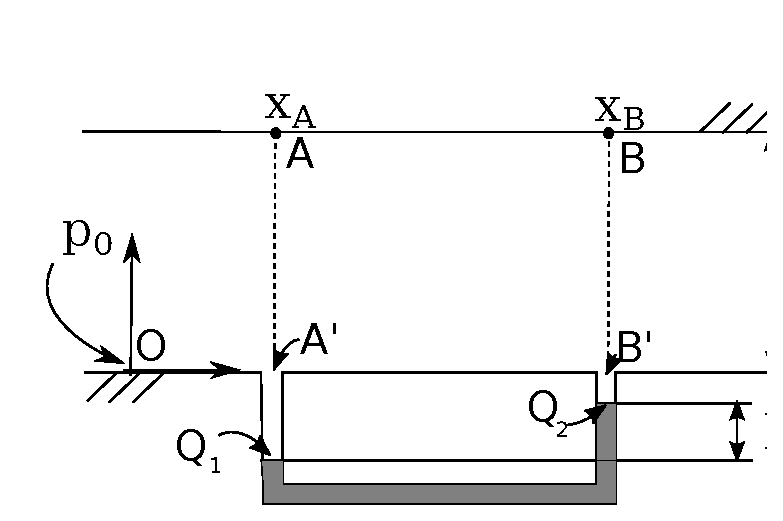
\includegraphics[width=0.90\textwidth]{./fig/manometro_Poiseuille.eps}
   \end{center}
\end{minipage}
\end{tabular}

\sol

\partone Soluzione esatte delle equazioni di Navier-Stokes. Corrente di
 Poiseuille nel canale piano 2D. Manometro: leggi della statica (Stevino).

\parttwo
\begin{itemize}
\item
Per trovare la derivata in direzione $x$ della pressione all'interno del
 canale ($\partial P/\partial x = - G_P = cost.$ per la corrente di Poiseuille) risolve il problema di statica all'interno del manometro.
Facendo riferimento al disegno, si utilizza Stevino tra i punti $A'-Q_1$,
 $Q_1-Q_2$, $Q_2-B'$ e l'informazione di derivata della pressione costante
 in direzione $x$ all'interno del canale, tra $A'$ e $B'$.
\begin{equation}
 \begin{cases}
  p_{A'} = p_{Q_1} - \rho g z_{Q_1} \\
  p_{Q_1} - \bar{\rho} g z_{Q_1} =   p_{Q_2} - \bar{\rho} g z_{Q_2} \\
  p_{B'} = p_{Q_2} - \rho g z_{Q_2} \\
  p_{A'} - p_{B'} = G_P \Delta x
 \end{cases} \Rightarrow
  G_P = \dfrac{1}{\Delta x}(\bar{\rho}-\rho) g \Delta h
\end{equation}
avendo svolto correttamente i conti e riconosciuto $z_{Q_2} - z_{Q_1} =
 \Delta h$.

\item
Ricordando che il profilo di velocità di Poiseuille risulta
 $\bm{u} = \bm{\hat{x}} u(y)$, con 
\begin{equation}
 u(y) = -\dfrac{G_P}{2 \mu} y (y-H),
\end{equation}
 la velocità massima all'interno del canale è $V = u(H/2) =
 \dfrac{G_P}{8 \mu} H^2$

\item
Per calcolare la risultante degli sforzi sul tratto $A-B$ della parete 
 superiore, è necessario calcolare il vettore sforzo agente su di essa
 e svolgere un semplice integrale.
Il vettore sforzo agente sulla parete superiore risulta
 \begin{equation}
  \bm{t} = - \mu \dfrac{\partial u}{\partial y}\bigg|_{y=H} \bm{\hat{x}} +
           p(x,H) \bm{\hat{y}} \ .
 \end{equation}
 La pressione $p(x,H)$ sulla parete superiore, per $x \in [x_A,x_B]$ si
 calcola come segue: si parte dall'origine del sistema di riferimento $O$,
 in corrispondenza della quale è noto il valore della pressione $p_0$ e ci 
 si muove in orizzontale ricordando che $\partial P/\partial x = -G_P$ e
 in verticale ricordando che $\partial P/\partial y = -\rho g$.
 \begin{equation}
 \begin{aligned}
  p_{A'} & = p_0 - G_P x_A \\
  p_{A } & = p_{A'} - \rho g H  \\
%  p_{B } & = p_{A}  - G_P (x_B - x_A)  \\ \\
 \end{aligned}
 \qquad \rightarrow  \qquad p(x,H)  = p_{A} - G_P ( x  -x_A )
 \end{equation}
 Lo sforzo tangenziale sulla parete è costante e vale
 \begin{equation}
  - \mu \dfrac{\partial u}{\partial y}\bigg|_{y=H} =
    \dfrac{G_P}{2} H
 \end{equation}
 La risultante delle forze (per unità di lunghezza, poichè il problema
  è bidimensionale) si ottiene integrando lo sforzo tra $A$ e $B$. Facendo comparire il valore $p_B$ della pressione in $B$, l'espressione della risultante delle forze diventa
 \begin{equation}
  \bm{R} = \dfrac{G_P}{2} H \Delta x \bm{\hat{x}} + 
           \dfrac{1}{2}(p_A + p_B) \Delta x \bm{\hat{y}} \ .
 \end{equation}


\end{itemize}
 % 2d channel + p meas.
\newpage
\noindent
\begin{tabular}{cc}
\begin{minipage}[c]{0.60\textwidth}
\begin{exerciseS}[Corrente libera su parete inclinata]
Si consideri una corrente d'acqua a pelo libero, laminare e stazionaria, che
scorre su una parete piana di lunghezza e apertura infinita  inclinata di un angolo $\alpha$ rispetto all'orizzontale.
Sul pelo libero la pressione è uniforme e uguale a $P_a$. Lo sforzo tangenziale fra acqua e aria viene considerato nullo.

Si calcoli il profilo di velocità nello strato di acqua e il campo di pressione.
\end{exerciseS}
\end{minipage}
\begin{minipage}[c]{0.35\textwidth}
   \begin{center}
   \includegraphics[width=0.90\textwidth]{./fig/slnEsatte-scivolo}
   \end{center}
\end{minipage}
\end{tabular}

\sol

\partone
 Semplificazione delle equazioni di NS in casi particolari. 
Soluzioni esatte in coordinate cartesiane.

\parttwo
Si scelga un sistema di riferimento cartesiano con l'asse $x$ orientato lungo la parete verso il basso e l'asse y perpendicolare ed uscente ad essa.
Sulla corrente di questo problema agiscono le forze di volume dovute alla gravità.
L'ipotesi che la pressione sia uniforme sulla superficie di interfaccia
 tra acqua e aria implica che la pressione è indipendente dalla coordinata $x$ in tutto il fluido.
% : si dimostra che $\dfrac{\partial p}{\partial y}=0$; se sulla superficie libera la pressione è costante e non varia nello spessore, allora la pressione è costante in tutto il fluido.

\begin{itemize}

   \item Scrittura delle equazioni di NS in coordinate cartesiane in 2 dimensioni.
%  
 \begin{equation}
\begin{cases}
  \dfrac{\partial u}{\partial t} + u \dfrac{\partial u}{\partial x}
  + v \dfrac{\partial u}{\partial y} - \nu \left( 
  \dfrac{\partial^2 u}{\partial x^2} +
  \dfrac{\partial^2 u}{\partial y^2} \right)
  + \dfrac{1}{\rho} \dfrac{\partial p}{\partial x} = f_x \\
  \dfrac{\partial v}{\partial t} + u \dfrac{\partial v}{\partial x}
  + v \dfrac{\partial v}{\partial y} - \nu \left( 
  \dfrac{\partial^2 v}{\partial x^2} +
  \dfrac{\partial^2 v}{\partial y^2} \right)
  + \dfrac{1}{\rho} \dfrac{\partial p}{\partial y} = f_y \\
  \dfrac{\partial u}{\partial x} + \dfrac{\partial v}{\partial y} = 0
\end{cases}
\end{equation}

  \item Semplificazione delle equazioni di NS per il problema considerato. Vengono fatte le seguenti ipotesi:
\begin{itemize}
\item problema stazionario: $\dfrac{\partial}{\partial t} = 0$;
\item direzione $x$ omogenea (canale infinito in direzione $x$): $\dfrac{\partial u}{\partial x} = \dfrac{\partial v}{\partial x} = 0$; 
\begin{remark}
non si può dire altrettanto della pressione, a causa del ruolo che questa ha nelle equazioni di NS incomprimibili. Il campo di pressione può essere interpretato come un moltiplicatore di Lagrange necessario a imporre il vincolo di incomprimibilità. Inoltre, ad eccezione di alcune condizioni al contorno, non appare mai direttamente come pressione $p$ ma solamente con le sue derivate spaziali. Da un punto di vista più fisico, la differenza di pressione lungo il canale è la forzante che mette in moto il fluido in una corrente di Poiseuille.
\end{remark}
\item la condizione $\dfrac{\partial u}{\partial x} = 0$ inserita nel vincolo di incomprimibilità, implica $\dfrac{\partial v}{\partial y}=0$; poichè $\dfrac{\partial v}{\partial x}=\dfrac{\partial v}{\partial y}=0$ segue che $v = \text{cost} = 0$, poiché è nulla a parete per la condizione al contorno di adesione, $\bm{u} = \bm{0}$.
\item no forze di volume: $\bm{f} = \rho \bm{g} = \rho g \sin \alpha \bm{\hat{x}} - \rho g \cos \alpha \bm{\hat{y}}$.
\end{itemize}
%
Le equazioni di NS possono essere semplificate 
\begin{equation}
\begin{cases}
  - \mu \dfrac{\partial^2 u}{\partial y^2} = - \dfrac{\partial p}{\partial x} + \rho g \sin \alpha \\
  \dfrac{\partial p}{\partial y} = - \rho g \cos \alpha \ .
\end{cases}
\end{equation}

Dalla seconda segue che l'espressione del campo di pressione è
\begin{equation}
 p(x,y) = -\rho g y \cos \alpha + f(x) \ .
\end{equation}
L'espressione di $f(x)$ può essere calcolata imponendo la condizione al contorno sul pelo libero, $p(x,H) = P_a$,
\begin{equation}
 P_a = -\rho g H \cos \alpha + f(x) \qquad \rightarrow \qquad f(x) = P_a + \rho g H \cos \alpha \ .
\end{equation}
La funzione $f(x)$ è costante, senza dipendere dalla coordinata $x$. Di conseguenza, il campo di pressione dipende solo dalla coordinata $y$
\begin{equation}
 p(x,y) = P_a + \rho g ( H - y ) \cos \alpha \ ,
\end{equation}
e la derivata di $\partial p / \partial x$ è nulla. La componente $x$ dell'equazione della quantità di moto diventa quindi un'equazione ordinaria del secondo ordine
\begin{equation}
   \begin{cases}
    - \mu u''(y) = \rho g  \sin \alpha  \ , \ y \in[0,H] \\
    u(0) = 0  \\ u'(H) = 0 \ ,
  \end{cases}
\end{equation}
con le condizioni al contorno di adesione a parete e di sforzo di taglio nullo all'interfaccia tra aria ed acqua, $0=\tau(H)=\mu \dfrac{\partial u}{\partial y}(H)=\mu u'(H)$. La derivata parziale in $y$ è stata sostituita da quella ordinaria, poichè
 la velocità è solo funzione di $y$.
  
  \item Soluzione dell'equazione differenziale  con dati al contorno: si integra due volte e si impongono le condizioni al contorno per ottenere la componente $u$ del campo di velocità.
  \begin{equation}
   u(y) = - \dfrac{\rho g}{2 \mu} y( y - H ) \sin \alpha \ .
  \end{equation}
  
\end{itemize}

 % 2d free + gravitation
\newpage
\noindent
\begin{tabular}{cc}
\begin{minipage}[b]{0.95\textwidth}
\begin{exerciseS}[Corrente libera su parete verticale]
Si consideri una corrente d'acqua a pelo libero, laminare e stazionaria, che
scorre su una parete verticale piana di lunghezza e apertura infinita.
Si ipotizzi che la pressione atmosferica che agisce sul pelo libero sia
uniforme. Si ipotizzi inoltre che lo sforzo tangenziale fra acqua e aria in
corrispondenza del pelo libero sia nullo.

Assegnata la portata in massa per unit\`a di apertura 
$\overline{Q}=0.5\ kg/(ms)$, determinare
\begin{enumerate}
  \item lo spessore $h$ della corrente d'acqua;
  \item lo sforzo tangenziale a parete;
  \item la velocit\`a in corrispondenza del pelo libero;
  \item la velocit\`a media e il numero di Reynolds basato su tale velocit\`a
        media e sullo spessore della corrente.
\end{enumerate}
Si sostituisca poi al pelo libero una parete solida.
Si determini quale dovrebbe essere la velocit\`a di tale parete per ottenere
una portata nulla.

Dati: $\overline{\rho}= 999\ kg/m^3$, 
$\overline{\mu}= 1.15\ 10^{-3} kg/(ms)$.

($h=5.61\, 10^{-4}\  m$, $\tau = 5.494\ Pa$, $u(h)=1.339\ m/s$,
$\overline{U}=0.893\  m/s$, $ Re=434.8$, $U=-0.4464\ m/s$.)
\end{exerciseS}
\end{minipage}
\end{tabular}

\sol

\partone
 Semplificazione delle equazioni di NS in casi particolari. 
Soluzioni esatte in coordinate cartesiane.

\parttwo
Si scelga un sistema di riferimento cartesiano con l'asse x orientato lungo la parete verso il basso e l'asse y perpendicolare ed uscente ad essa.

\noindent
Sulla corrente di questo problema agisce la forza di volume dovuta alla gravità.  

L'ipotesi che la pressione sia uniforme sulla superficie di interfaccia
 tra acqua e aria implica che la pressione è costante in tutto il fluido:
 si vedrà che $\frac{\partial p}{\partial y}=0$; se sulla superficie libera
 la pressione è costante e non varia nello spessore, allora la pressione
 è costante in tutto il fluido.

\begin{itemize}

  \item Scrittura delle equazioni di NS in 2 dimensioni.
  
 \begin{equation}
\begin{cases}
  \frac{\partial u}{\partial t} + u \frac{\partial u}{\partial x}
  + v \frac{\partial u}{\partial y} - \nu \left( 
  \frac{\partial^2 u}{\partial x^2} +
  \frac{\partial^2 u}{\partial y^2} \right)
   + \frac{1}{\rho} \frac{\partial p}{\partial x} = f_x \\
  \frac{\partial v}{\partial t} + u \frac{\partial v}{\partial x}
  + v \frac{\partial v}{\partial y} - \nu \left( 
  \frac{\partial^2 v}{\partial x^2} +
  \frac{\partial^2 v}{\partial y^2} \right)
  + \frac{1}{\rho}  \frac{\partial p}{\partial y} = f_y \\
  \frac{\partial u}{\partial x} + \frac{\partial v}{\partial y} = 0
\end{cases}
\end{equation}

  \item Semplificazione delle equazioni di NS per il problema da affrontare.
  
Ipotesi: 
\begin{itemize}
\item problema stazionario: $\frac{\partial}{\partial t} = 0$;
\item direzione x omogenea (canale infinito in direzione x): $\frac{\partial u}{\partial x} = \frac{\partial v}{\partial x} = 0$; 
la pressione nelle equazioni di NS incomprimibili è un moltiplicatore di Lagrange per imporre il vincolo di incomprimibilità; inoltre non appare mai, se non nelle condizioni al contorno, come $p$ ma solo con le sue derivate spaziali: quindi non è corretto imporre $= \frac{\partial v}{\partial x} = 0$, nonostante la direzione $x$ sia omogenea;
\item $\frac{\partial u}{\partial x} = 0$ inserito nel vincolo di incomprimibilità ($\frac{\partial u}{\partial x}+\frac{\partial v}{\partial y}=0$) implica $\frac{\partial v}{\partial y}=0$; poichè $\frac{\partial v}{\partial x}=\frac{\partial v}{\partial y}=0$ e $v = 0$ a parete per la condizione al contorno di adesione, segue che $v = \text{cost} = 0$;
\item forze di volume solo in direzione verticale: per come sono stati orientati gli assi, $\bm{f} = g \hat{\bm{x}}$.
\end{itemize}
  
\begin{equation}
\begin{cases}
  - \mu \frac{\partial^2 u}{\partial y^2} = - \frac{\partial p}{\partial x} + \rho g\\
  \frac{\partial p}{\partial y} = 0  
\end{cases}
\end{equation}

Dalla seconda segue che la pressione può essere funzione solo di $x$. Come già detto in precedenza, la pressione sulla superficie libera è costante e uguale alla pressione ambiente $P_a$: se la pressione non può variare nello spessore, allora è costante ovunque. La derivata parziale $\frac{\partial p}
 {\partial x}=0$, il suo gradiente è nullo e quindi la pressione è costante
 in tutta la corrente di acqua.

 Nella prima, il termine a sinistra dell'uguale è funzione solo di $y$; quello di destra è costante e uguale a $\rho g$. Le condizioni al contorno sono
 di adesione a parete e di sforzo di taglio nullo all'interfaccia tra aria
 ed acqua: $0=\tau(H)=\mu \frac{\partial u}{\partial y}(H)=\mu u'(H)$, dove 
 la derivata parziale in $y$ è stata sostituita da quella ordinaria, poichè
 la velocità è solo funzione di $y$.
%  \begin{equation}
%  \end{equation}
  
  \begin{equation}
  \begin{cases}
    - \mu u''(y) = \rho g \ , \ y \in[0,H] \\
    u(0) = 0  \\ u'(H) = 0
  \end{cases}
  \end{equation}
  
  
  
  \item Soluzione dell'equazione differenziale (semplice) con dati al contorno.
  
  Risulta:
  \begin{equation}
    \Rightarrow u(y) = - \frac{\rho g}{2 \mu} y^2 + \frac{\rho g}{\mu} H y
  \end{equation}
  
  \item Calcolo della portata come integrale della velocità; si trova così la relazione tra Q ed H.
  
  \begin{equation}
    Q = \int_{0}^{H} \rho u(y) dy = \frac{1}{3}\frac{\rho^2 g}{\mu} H^3 
  \end{equation}
  E quindi
  \begin{equation}
     H = \left( \frac{3 Q \mu}{\rho^2 g} \right) ^ {\frac{1}{3}}
     \quad \Rightarrow \quad H = 5.61 \cdot 10^{-4} m
  \end{equation}
  
  \item Calcolo dello sforzo a parete
  \begin{equation}
    \tau = \mu u'|_{y=0} = \rho g H \quad \Rightarrow \quad \tau = 5.494 Pa
  \end{equation}
  \textit{Osservazione.} Equilibrio con la forza di gravità (problema stazionario).
  
  \item Calcolo di $u(H)$.
  \begin{equation}
    u(H) = \frac{1}{2}\frac{\rho g}{\mu} H^2 
    \quad \Rightarrow \quad u(H) = 1.342 m/s
  \end{equation}
  
  \item Calcolo velocità media e numero di Reynolds.
  \begin{equation}
    \bar{U} = \frac{1}{H}\int_{0}^{H} u(y) dy = \frac{Q}{\rho H}
    \quad \Rightarrow \quad \bar{U} = \frac{Q}{\rho H}
                                    = \frac{2}{3}u(H) = 0.895 m/s
  \end{equation}
  
  \begin{equation}
    Re = \frac{\rho \bar{U} H}{\mu}
    \quad \Rightarrow \quad Re = 434.8
  \end{equation}
 
  
\end{itemize}

L'ultima parte del problema chiede di sostiutire alla superficie libera,
 una parete infinita. L'equazione trovata in precedenza è ancora valida;
 è necessario però sostituire la condizione di sforzo tangenziale nullo
 con adesione su una parete mobile con velocità costante $U$.

  \begin{equation}
  \begin{cases}
    - \mu u''(y) = \rho g \ , \ y \in[0,H] \\
    u(0) = 0  \\ u(H) = U
  \end{cases}
  \end{equation}

Il profilo di velocità è:
\begin{equation}
 u(y) = \dfrac{\rho g}{2 \mu}(-y^2 + yH) +\dfrac{U}{H}y
\end{equation}
dove la velocità $U$ è ancora incognita. Per trovarne il valore, si 
calcola la portata e la si pone uguale a zero. La portata è uguale a
\begin{equation}
 Q = \int_0^H u(y) dy = \dots = \dfrac{1}{12}\dfrac{\rho g H^3}{\mu}
 + \dfrac{1}{2}UH
\end{equation}
Imponendo $Q=0$,
\begin{equation}
 U = - \dfrac{\rho g H^2}{6 \mu} \quad \Rightarrow \quad
 U = - 0.4474\ m/s
\end{equation}

 % 2d free + gravitation
\newpage
\noindent
\begin{tabular}{cc}
\begin{minipage}[b]{0.60\textwidth}
\begin{exerciseS}[Corrente di Poiseuille in un tubo a sezione circolare e manometro]
Un manometro a mercurio ($\rho_{hg} = 13610 \  kg/m^3$)
collega due prese di pressione posizionate a una distanza di $l = 2 \ 
m$ l'una dall'altra lungo un tubo orizzontale di diametro $2R = 5 \ cm$
 in cui scorre un fluido con densità $\rho_{f} = 950 \
kg/m^3$. Se la differenza fra le altezze dei peli liberi del 
liquido manometrico nelle due colonne
vale $\Delta h = 4 \ cm$ e la portata volumetrica che scorre nel tubo è 
$Q= 6\ m^3/s$,
quanto valgono la viscosità $\mu$ del fluido e lo sforzo a parete
$\tau_w$?

($\mu = 6.36\,10^{-5} \ kg/(m\, s)$,
$\tau_w = 31.05\, \bm{z}\ N/m^2$)
\end{exerciseS}
\end{minipage}
&
\begin{minipage}[b]{0.35\textwidth}
   \begin{center}
   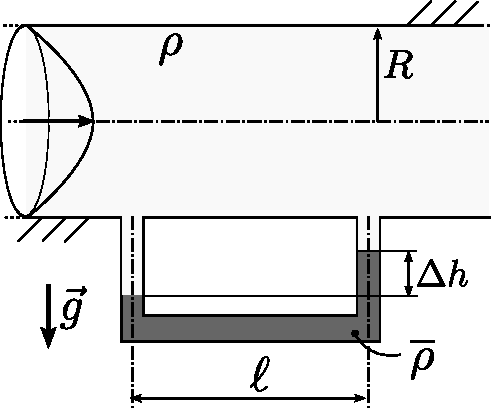
\includegraphics[width=0.90\textwidth]{./fig/slnEsatte-poiseuille}
   \end{center}
\end{minipage}
\end{tabular}


\sol

\partone Semplificazione delle equazioni di NS in casi particolari. 
Soluzioni esatte in coordinate cilindriche. Legge di Stevino.

Scrittura del contributo viscoso del vettore sforzo come:
\begin{equation}
\begin{aligned}
  \bm{s_n} & = \mathbb{S} \cdot \bm{\hat{n}} = \\
           & = \mu [\bm{\nabla} \bm{u} + \bm{\nabla}^T \bm{u}] \cdot \bm{\hat{n}} = \\
           & = \mu \left[ 2 (\bm{\hat{n}} \cdot \bm{\nabla} ) \bm{u} + \bm{\hat{n}} \times \bm{\nabla} \times \bm{u}  \right]
\end{aligned}
\end{equation}

\parttwo La geometria del problema suggerisce di utilizzare un sistema di coordiante cilindriche.

\begin{itemize}
  \item Scrittura delle equazioni di NS in coordinate cilindriche
  \begin{equation}
  \begin{cases}
    \rho \dfrac{\partial u_r}{\partial t}
    + \rho \left( \bm{u} \cdot \bm{\nabla}u_r - \dfrac{u_\theta^2}{r} \right)
    - \mu \left(\nabla^2 u_r 
       - \dfrac{u_r}{r^2} 
       - \dfrac{2}{r^2}\dfrac{\partial u_\theta}{\partial \theta} \right)  
       + \dfrac{\partial p}{\partial r} = f_r \\
    \rho \dfrac{\partial u_\theta}{\partial t}
    + \rho \left( \bm{u} \cdot \bm{\nabla} u_\theta + \dfrac{u_\theta u_r}{r} \right)
    - \mu \left(\nabla^2 u_\theta 
       - \dfrac{u_\theta}{r^2} 
       + \dfrac{2}{r^2}\dfrac{\partial u_r}{\partial \theta}  \right) 
    + \dfrac{1}{r} \dfrac{\partial p}{\partial \theta} = f_\theta\\
    \rho \dfrac{\partial u_z}{\partial t}
    + \rho \bm{u} \cdot \bm{\nabla} u_z
    - \mu \nabla^2 u_z
    + \dfrac{\partial p}{\partial z} = f_z \\ \\
    \dfrac{1}{r}\dfrac{\partial}{\partial r}\left( r u_r \right) 
    + \dfrac{1}{r}\dfrac{\partial u_\theta}{\partial \theta} 
    + \dfrac{\partial u_z}{\partial z} = 0
  \end{cases}
  \end{equation}
  con 
  \begin{equation}
  \begin{aligned}
  & \bm{a} \cdot \bm{\nabla} b = a_r \dfrac{\partial b}{\partial r} 
     + \dfrac{a_\theta}{r} \dfrac{\partial b}{\partial \theta}  
     + a_z \dfrac{\partial b}{\partial z} \\
  & \nabla^2 f = \dfrac{1}{r}\dfrac{\partial}{\partial r}
                      \left(r \dfrac{\partial f}{\partial r} \right) +
               \dfrac{1}{r^2} \dfrac{\partial^2 f}{\partial \theta^2} + 
               \dfrac{\partial^2 f}{\partial z^2} 
  \end{aligned}
  \end{equation}
%  \begin{equation}
%  \begin{cases}
%   {} \\
%   ... \\
%   {}
%  \end{cases}
%  \end{equation}
  
  \item Semplificazione delle equazioni di NS per il problema considerato. Vengono fatte le sequenti ipotesi:
\begin{itemize}
\item problema stazionario: $\dfrac{\partial}{\partial t} = 0$;
\item direzione z omogenea (canale infinito in direzione z): $\dfrac{\partial u}{\partial z} = \dfrac{\partial v}{\partial z} = 0$; come discusso negli esercizi in geometria cartesiana, il termine $\dfrac{\partial P}{\partial z} = - G_P$ è costante e in generale diverso da zero.

\item problema assialsimmetrico: $\dfrac{\partial}{\partial \theta} = 0$;
\item no swirl: $u_{\theta} = 0$;
\item dall'incomprimibilità e dalle condizioni al contorno a parete, segue che la componente radiale della velocità è identicamente nulla, $u_r = 0$;
\item no forze di volume: $\bm{f} = 0$.
\end{itemize}

Grazie alle ipotesi fatte, il campo di velocità assume la forma $\bm{u}(\bm{r}) = u(r) \bm{\hat{z}}$. La componente radiale e azimuthale dell'equazione della quantità di moto sono identicamente soddisfatte, mentre la componente lungo $z$ diventa
\begin{equation}
  \begin{cases}
     \mu \dfrac{1}{r} \dfrac{d}{dr}\left( r \dfrac{d}{dr} u(r)\right) = -G_P & r \in[0,R] \\
    u(0) = $valore finito$  \\ u(R) = 0
  \end{cases}
  \end{equation}
dove la derivata ordinaria $\dfrac{d}{d r}$ è stata utilizzata al posto della derivta parziale, poichè la componente assiale della velocità dipende solamente dalla coordinata radiale, $u(r)$. Le condizioni al contorno garantiscono che il campo di velocità sia regolare nel dominio (in particolare che non esistano singolarità sull'asse) e che sia soddisfatta la condizione al contorno di adesione a parete.

\item Soluzione dell'equazione differenziale. Si integra due volte e si ottiene:
\begin{equation}
  u(r) = -\dfrac{G_P}{4 \mu} r^2 + A \ln{r} + B
\end{equation}
Imponendo le condizioni al contorno, $A$ deve essere nullo per l'ipotesi di valore finito in $r=0$ ($\ln r \rightarrow -\infty$ quando $r \rightarrow 0$). Imponendo poi la condizione di adesione a parete per $r=R$, si ottiene:
\begin{equation}
  u(r) = -\dfrac{G_P}{4 \mu} (r^2 - R^2) \ .
\end{equation}

\item Calcolo della portata: si integra la velocità sulla sezione circolare (\textbf{!}) del tubo. Questa relazione lega il gradiente di pressione $G_P$ alla portata $Q$ e al coefficiente di viscosità dimanica $\mu$,
\begin{equation}
  Q = \int_{\theta=0}^{2\pi} \int_{r=0}^{R} u(r) r dr d\theta = 
  2\pi \int_{r=0}^{R} u(r) r dr =
  \dfrac{\pi}{8}\dfrac{G_P R^4}{\mu} \ .
\end{equation}

La differenza di pressione tra i due punti A e B (separati da una distanza $l$) è quindi $P_B - P_A = -G_P l$.

\item Applicazione della legge di Stevino per ottenere il sistema risolvente:
\begin{equation}
\begin{cases}
  P_1 = P_A + \rho_f g H_0 & \text{(Stevino tra 1 e A)} \\
  P_2 = P_B + \rho_f g (H_0-\Delta h) & \text{(Stevino tra 2 e B)} \\
  P_B = P_A - G_P l & \text{(relazione trovata dalla sln di NS)} \\
  P_2 = P_1 - \rho_{Hg} g \Delta h & \text{(Stevino tra 1 e 2)}
\end{cases}
\end{equation}

Risolvendo il sistema, si trova che:
\begin{equation}
  G_P l = (\rho_{Hg} - \rho_f) g \Delta h
\end{equation}

Esplicitando il legame tra $G_P$ e $\mu$, si ottiene il risultato:
\begin{equation}
  \Rightarrow \quad \mu = \dfrac{\pi R^4}{8 Q l} (\rho_{Hg} - \rho_f) g \Delta h \quad \Rightarrow \quad \mu = 6.36 \cdot 10^{-5} \dfrac{kg}{m s}
\end{equation}

\item Bisogna calcolare ora $\tau_w$,la componente parallela alla parete dello sforzo a parete. Usando l'espressione vettoriale della parte viscosa del vettore sforzo agente sul fluido (aiutandosi con le tabelle per le espressioni in coordinate cilindriche degli operatori differenziali) con $\bm{u} = u_z(r)\bm{\hat{z}}$ e $\bm{\hat{n}} = \bm{\hat{r}}$, si può scrivere
\begin{equation}
\begin{aligned}
   \bm{s_n} & = \mu \left[ 2 (\bm{\hat{n}} \cdot \bm{\nabla} ) \bm{u} + \bm{\hat{n}} \times \bm{\nabla} \times \bm{u}  \right] = \\
            & = \mu \left[ 2 \dfrac{\partial u_z}{\partial r}\bm{\hat{z}} - \dfrac{\partial u_z}{\partial r} \bm{\hat{z}} \right] = \\
            & = \mu \dfrac{\partial u_z}{\partial r}\bm{\hat{z}} \ .
\end{aligned}
\end{equation}
%
Ricordando che lo sforzo agente sulla parete è uguale e contrario a quello agente sul fluido e che lo sforzo dovuto alla pressione è normale alla parete, 
\begin{equation}
\begin{aligned}
   \tau_w & = - \mu \dfrac{\partial u_z}{\partial r}\bigg|_{r=R} = \\
          & = \dfrac{1}{2} G_P R \ .
\end{aligned}
\end{equation}
%
Si ottiene quindi il valore, $\tau_w = 31.05 N/m^2$.
\end{itemize}

\begin{remark}
 L'espressione dello sforzo tangenziale a parete $\tau_w = - \mu \frac{\partial u_z}{\partial r}$ per la corrente di Poiseuille in un tubo a sezione circolare è simile a quella ottenuta per la corrente in un canale piano, in coordinate cartesiane, $\tau_w = \mu \frac{\partial u}{\partial y}$. In questi due casi, la componente tangenziale dello sforzo è proporzionale alla derivata in direzione perpendicolare alla parete della componente di velocità parallela alla parete. Questa \textbf{NON} è una formula generale per lo sforzo tangenziale a parete, come sarà evidente nel caso della corrente di Taylor-Couette.
\end{remark}

 % 3d poiseuille + p meas.
\newpage
\noindent
\begin{tabular}{cc}
\begin{minipage}{0.60\textwidth}
\begin{exerciseS}[Corrente di Taylor-Couette]
Si consideri la corrente piana fra due cilindri coassiali rotanti.
Si misura la velocit\`a in due punti posti rispettivamente a $1/4$ e 
$3/4$ del gap fra i due cilindri: 
$u_{\theta,1/4} = 0.5\ m/s$, 
$u_{\theta,3/4} = 0.8\ m/s$.
Si determini la velocit\`a di rotazione dei due cilindri nonch\'e
la pressione in corrispondenza del cilindro interno sapendo che
la pressione in corrispondenza del cilindro esterno vale $5\ Pa$,
che la densit\`a del fluido \`e pari a $1.225\ kg/m^3$,
che il diametro del cilindro interno \`e $d =2 R_1=0.1 \ m$ e che il diametro 
del cilindro esterno \`e $D = 2 R_2 = 0.16 \ m$.
 
($\Omega_{1}=6.663\ s^{-1}$, $\Omega_{2}=11.743\ s^{-1}$ \newline
$P(r) = P_2 - \rho \left[ \dfrac{1}{2} A^2 (R_2^2 - r^2) + 2 A B ln \dfrac{R_2}{r} - 
      \dfrac{1}{2}B^2 \left( \dfrac{1}{R^2} - \dfrac{1}{r^2} \right)  \right]$, \newline
      con $u_{\theta}(r) = A r + B/r$\ .
 )
\end{exerciseS}
\end{minipage}
&
\begin{minipage}{0.35\textwidth}
   \begin{center}
   \includegraphics[width=0.90\textwidth]{./fig/slnEsatte-taylor-couette-2}
   \end{center}
\end{minipage}
\end{tabular}

\sol

\partone Soluzione esatte delle equazioni di Navier-Stokes in geometria cilindrica. Corrente di Taylor-Couette.

\begin{equation}
  \begin{cases}
    \rho \dfrac{\partial u_r}{\partial t}
    + \rho \left( \bm{u} \cdot \bm{\nabla}u_r - \dfrac{u_\theta^2}{r} \right)
    - \mu \left(\nabla^2 u_r 
       - \dfrac{u_r}{r^2} 
       - \dfrac{2}{r^2}\dfrac{\partial u_\theta}{\partial \theta} \right)  
       + \dfrac{\partial p}{\partial r} = f_r \\
    \rho \dfrac{\partial u_\theta}{\partial t}
    + \rho \left( \bm{u} \cdot \bm{\nabla} u_\theta + \dfrac{u_\theta u_r}{r} \right)
    - \mu \left(\nabla^2 u_\theta 
       - \dfrac{u_\theta}{r^2} 
       + \frac{2}{r^2}\dfrac{\partial u_r}{\partial \theta}  \right) 
    + \dfrac{1}{r} \frac{\partial p}{\partial \theta} = f_\theta\\
    \rho \dfrac{\partial u_z}{\partial t}
    + \rho \bm{u} \cdot \bm{\nabla} u_z
    - \mu \nabla^2 u_z
    + \dfrac{\partial p}{\partial z} = f_z \\ \\
    \dfrac{1}{r}\dfrac{\partial}{\partial r}\left( r u_r \right) 
    + \dfrac{1}{r}\dfrac{\partial u_\theta}{\partial \theta} 
    + \dfrac{\partial u_z}{\partial z} = 0
  \end{cases}
  \end{equation}
  con 
  \begin{equation}
  \begin{aligned}
  & \bm{a} \cdot \bm{\nabla} b = a_r \dfrac{\partial b}{\partial r} 
     + \dfrac{a_\theta}{r} \dfrac{\partial b}{\partial \theta}  
     + a_z \dfrac{\partial b}{\partial z} \\
  & \nabla^2 f = \dfrac{1}{r}\dfrac{\partial}{\partial r}
                      \left(r \frac{\partial f}{\partial r} \right) +
               \frac{1}{r^2} \frac{\partial^2 f}{\partial \theta^2} + 
               \frac{\partial^2 f}{\partial z^2} 
  \end{aligned}
  \end{equation}

\parttwo Il problema viene risolto calcolando prima le velocità angolari dei cilindri e
successivamente la pressione.

\begin{itemize}

\item La soluzione di Taylor-Couette viene ricavata dall'espressione semplificata delle equazioni di Navier-Stokes,
\begin{equation}
\begin{cases}
  -\rho \dfrac{u^2_\theta}{r} + \dfrac{\partial P}{\partial r} = 0 \\
  -\dfrac{1}{r}\dfrac{\partial}{\partial r} \left( r \dfrac{\partial u_\theta}{\partial r}  \right)  + \dfrac{u_\theta}{r^2}= 0 \ ,
\end{cases}
\end{equation}
ottenute imponendo che il campo di moto sia bidimensionale $\bm{u}(\bm{r}) = u_{\theta}(r,\theta) \bm{\hat{\theta}} + u_r (r,\theta) \bm{\hat{r}}$, che la soluzione sia omogenea rispetto alla coordinata $\theta$ e sfruttando le condizioni al contorno e il vincolo di incomprimibilità per ricavare $u_r(\theta) = 0$.
%
Sia il campo di pressione sia il campo di velocità dipendono solamente dalla coordinata radiale, $P = P(r)$, $u_\theta = u_\theta (r)$. Le derivate parziali possono essere quindi trasformate in derivate ordinarie. La seconda equazione è disaccoppiata dalla prima e può essere risolta, una volta imposte le condizioni al contorno. Trovato il campo di moto da questa equazione, la prima viene usata per calcolare il campo di pressione. La seconda equazione può essere riscritta come (svolgere le derivate per credere!)
\begin{equation}
\begin{cases}
  -\left(\dfrac{1}{r} \left(r u_\theta\right)'\right)' = 0 \\
  u_\theta(R_1) = \Omega_1 R_1 \\
  u_\theta(R_2) = \Omega_2 R_2 \\
\end{cases}
\Rightarrow
\begin{cases}
  u_\theta(r) = A r + \dfrac{B}{r} \ \ \ \text{A,B from b.c.} \\
  u_\theta(R_1) = \Omega_1 R_1 \\
  u_\theta(R_2) = \Omega_2 R_2 \\
\end{cases}
\end{equation}
%
Il campo di moto tra due cilindri coassiali rotanti è
\begin{equation}
  u_\theta(r) = \frac{\Omega_2 R_2^2 - \Omega_1 R_1^2}{R_2^2-R_1^2} r +
   \frac{(\Omega_1 - \Omega_2)R_1^2 R_2^2}{R_2^2-R_1^2}\frac{1}{r} \ .
\end{equation}
%
\begin{remark} La soluzione esatta di Taylor-Couette è facile da ricavare, se si ricorda
che è la somma di una rotazione rigida e un vortice irrotazionale: imponendo la forma
$u_\theta (r) = A r + B/r$ e le condizioni al contorno,
\begin{equation}
 u_{\theta}(R_1) = \Omega_1 R_1 \qquad , \qquad  u_{\theta}(R_2) = \Omega_2 R_2
\end{equation}
si ottiene la formula voluta.
\end{remark}

\item Calcolo delle velocità angolari dei cilindri. Nota la forma del campo di moto e
le velocità in due punti a diversi raggi, è possibile calcolare $\Omega_1$, $\Omega_2$
 risolvendo un sistema lineare di due equazioni nelle due incognite.
%
Note le misure di velocità $u_{\theta,1/4} = u_{\theta}(r_{1/4})$, $u_{\theta,3/4} = u_{\theta}(r_{3/4})$, il sistema risolvente diventa:
\begin{equation}
 \displaystyle\begin{bmatrix}
  -\frac{R_1^2}{R_2^2-R_1^2}r_{1/4} + \frac{R_1^2 R_2^2}{R_2^2-R_1^2}\frac{1}{r_{1/4}} & \quad
   \frac{R_2^2}{R_2^2-R_1^2}r_{1/4} - \frac{R_1^2 R_2^2}{R_2^2-R_1^2}\frac{1}{r_{1/4}} \\ 
  -\frac{R_1^2}{R_2^2-R_1^2}r_{3/4} + \frac{R_1^2 R_2^2}{R_2^2-R_1^2}\frac{1}{r_{3/4}} & \quad
   \frac{R_2^2}{R_2^2-R_1^2}r_{3/4} - \frac{R_1^2 R_2^2}{R_2^2-R_1^2}\frac{1}{r_{3/4}} \\
 \end{bmatrix}
 \displaystyle\begin{bmatrix}
  \Omega_1 \\ \Omega_2
 \end{bmatrix} =
 \displaystyle\begin{bmatrix}
  u_{\theta,1/4} \\ u_{\theta,3/4}
 \end{bmatrix}
\end{equation}

%La soluzione di Taylor-Couette può essere ricavata abbastanza facilmente semplificando le  equazioni di Navier-Stokes scritte in coordinate cilindriche, dopo aver fatto le opportune ipotesi (quali?). Le componenti in direzione radiale e tangenziale dell'equazione della quantità di moto diventano:

\item Calcolo della pressione. Una volta noto il campo di moto, è possibile calcolare il campo di pressione dalla componente radiale dell'equazione della quantità di moto,
\begin{equation}
\begin{aligned}
  P'(r) & = \rho \dfrac{u_\theta^2}{r} \quad , \quad \text{con $P(R_2) = P_2$} \\
 & \quad \rightarrow \quad
 \int_{r}^{R_2} \dfrac{dP}{dr} dr 
      = \int_r^{R_2} \rho \dfrac{1}{r} \left( A r + \dfrac{B}{r} \right)^2 dr
\end{aligned}
\end{equation}
%
Da questa si ricava
\begin{equation}
  P(r) = P_2 - \rho \left[ \dfrac{1}{2} A^2 (R_2^2 - r^2) + 2 A B ln \dfrac{R_2}{r} - 
      \dfrac{1}{2}B^2 \left( \dfrac{1}{R^2} - \dfrac{1}{r^2} \right)  \right] \ .
\end{equation}


\end{itemize}

 % taylor-couette + p meas.
\newpage
\noindent
\begin{tabular}{cc}
\begin{minipage}{0.60\textwidth}
\begin{exerciseS}[Corrente di Taylor-Couette: coppia sui cilindri]
Si consideri la corrente piana di un fluido di densità $\rho$ fra due cilindri coassiali di raggio $R_1$ e $R_2$. Il cilindro esterno è fermo, mentre quello interno è messo in rotazione da un motore con curva caratteristica $C_{disp}(\Omega) = \alpha - \beta \Omega$.
Si determini il punto di equilibrio del sistema ($\Omega$ costante).
 
(\dots)
\end{exerciseS}
\end{minipage}
&
\begin{minipage}{0.35\textwidth}
   \begin{center}
   \includegraphics[width=0.95\textwidth]{./fig/slnEsatte-taylor-couette}
   \end{center}
\end{minipage}
\end{tabular}

\sol

\partone Soluzione esatte delle equazioni di Navier-Stokes in geometria cilindrica. Corrente di Taylor-Couette.

\begin{equation}
  \begin{cases}
    \rho \dfrac{\partial u_r}{\partial t}
    + \rho \left( \bm{u} \cdot \bm{\nabla}u_r - \dfrac{u_\theta^2}{r} \right)
    - \mu \left(\nabla^2 u_r 
       - \dfrac{u_r}{r^2} 
       - \dfrac{2}{r^2}\dfrac{\partial u_\theta}{\partial \theta} \right)  
       + \dfrac{\partial p}{\partial r} = f_r \\
    \rho \dfrac{\partial u_\theta}{\partial t}
    + \rho \left( \bm{u} \cdot \bm{\nabla} u_\theta + \dfrac{u_\theta u_r}{r} \right)
    - \mu \left(\nabla^2 u_\theta 
       - \dfrac{u_\theta}{r^2} 
       + \frac{2}{r^2}\dfrac{\partial u_r}{\partial \theta}  \right) 
    + \dfrac{1}{r} \frac{\partial p}{\partial \theta} = f_\theta\\
    \rho \dfrac{\partial u_z}{\partial t}
    + \rho \bm{u} \cdot \bm{\nabla} u_z
    - \mu \nabla^2 u_z
    + \dfrac{\partial p}{\partial z} = f_z \\ \\
    \dfrac{1}{r}\dfrac{\partial}{\partial r}\left( r u_r \right) 
    + \dfrac{1}{r}\dfrac{\partial u_\theta}{\partial \theta} 
    + \dfrac{\partial u_z}{\partial z} = 0
  \end{cases}
  \end{equation}
  con 
  \begin{equation}
  \begin{aligned}
  & \bm{a} \cdot \bm{\nabla} b = a_r \dfrac{\partial b}{\partial r} 
     + \dfrac{a_\theta}{r} \dfrac{\partial b}{\partial \theta}  
     + a_z \dfrac{\partial b}{\partial z} \\
  & \nabla^2 f = \dfrac{1}{r}\dfrac{\partial}{\partial r}
                      \left(r \frac{\partial f}{\partial r} \right) +
               \frac{1}{r^2} \frac{\partial^2 f}{\partial \theta^2} + 
               \frac{\partial^2 f}{\partial z^2} 
  \end{aligned}
  \end{equation}
  
\vspace{0.5cm}
Espressione vettoriale del contributo viscoso del vettore sforzo,
\begin{equation}
\begin{aligned}
  \bm{s_n} & = \mathbb{S} \cdot \bm{\hat{n}} = \\
           & = \mu [\bm{\nabla} \bm{u} + \bm{\nabla}^T \bm{u}] \cdot \bm{\hat{n}} = \\
           & = \mu \left[ 2 (\bm{\hat{n}} \cdot \bm{\nabla} ) \bm{u} + \bm{\hat{n}} \times \bm{\nabla} \times \bm{u}  \right]
\end{aligned}
\end{equation}

\parttwo Viene risolto il problema piano, nel quale i campi di velocità e di pressione hanno la forma 
\begin{equation}
 \bm{u}(\bm{r}) = u_r(r,\theta) \bm{\hat{r}} + u_{\theta}(r,\theta) \bm{\hat{\theta}} \quad , \quad P(\bm{r}) = P(r,\theta) \ ,
\end{equation}
e le azioni integrali (come la coppia fornita e quella incognita) sono intese per unità di lunghezza, essendo la ``dimensione mancante'' quella fuori dal piano del disegno.

\begin{itemize}

\item Calcolo delle velocità angolari dei cilindri. Nota la forma del campo di moto e
le velocità in due punti a diversi raggi, è possibile calcolare $\Omega_1$, $\Omega_2$
 risolvendo un sistema lineare di due equazioni nelle due incognite.
%
Il campo di moto tra due cilindri coassiali rotanti è:
\begin{equation}
  u_\theta(r) = A r + \dfrac{B}{r} = \frac{\Omega_2 R_2^2 - \Omega_1 R_1^2}{R_2^2-R_1^2} r +
   \frac{(\Omega_1 - \Omega_2)R_1^2 R_2^2}{R_2^2-R_1^2}\frac{1}{r} \ .
\end{equation}
Se il cilindro esterno è fermo e la velocità angolare del cilindro interno vale $\Omega_1 = \Omega$, i coefficienti $A$ e $B$ valgono
\begin{equation}
 A = - \frac{R_1^2}{R_2^2-R_1^2} \Omega  < 0 \qquad , \qquad B = \frac{R_1^2 R_2^2}{R_2^2-R_1^2} \Omega > 0 \ .	
\end{equation}
%
\begin{remark} La soluzione esatta di Taylor-Couette è facile da ricavare, se si ricorda
che è la somma di una rotazione rigida e un vortice irrotazionale: imponendo la forma
$u_\theta (r) = A r + B/r$ e le condizioni al contorno,
\begin{equation}
 u_{\theta}(R_1) = \Omega_1 R_1 \qquad , \qquad  u_{\theta}(R_2) = \Omega_2 R_2
\end{equation}
si ottiene la formula voluta.
\end{remark}

\item Calcolo dello sforzo tangenziale a parete per determinare il puto di equilibrio del sistema. Si determina la componente tangenziale (quella che contribuisce alla coppia resistente)
dello sforzo sul cilindro interno.
Il contributo viscoso del vettore sforzo può essere scritto come:
\begin{equation}
\begin{aligned}
  \bm{s_n} & = \mathbb{S} \cdot \bm{\hat{n}} = \\
           & = \mu [\bm{\nabla} \bm{u} + \bm{\nabla}^T \bm{u}] \cdot \bm{\hat{n}} = \\
           & = \mu \left[ 2 (\bm{\hat{n}} \cdot \bm{\nabla} ) \bm{u} + \bm{\hat{n}} \times \bm{\nabla} \times \bm{u}  \right] = &  \text{(verificare con le tabelle)} \\
           & = \mu \left[ 2 \dfrac{\partial u_\theta}{\partial r} - \dfrac{1}{r} 
    \dfrac{\partial}{\partial r} (r u_\theta) \right] \bm{\hat{\theta}} = \\
           & = \mu \left[ \dfrac{\partial u_\theta}{\partial r} - \dfrac{u_\theta}{r} \right] \bm{\hat{\theta}} = &  \text{($u_\theta = A r + B / r$)}\\
           & = - 2 \mu \dfrac{B}{r^2} \bm{\hat{\theta}} 
\end{aligned}
\end{equation}
%
\begin{remark}
 La formula dello sforzo tangenziale a parete per la corrente di Taylor-Couette è $\tau_w = \mu \left[ \frac{\partial u_\theta}{\partial r} - \frac{u_\theta}{r} \right]$,
\end{remark}
%
La parte tangenziale dello sforzo a parete sul cilindro interno è quindi $\tau_w = 
2 \mu {B}/{R_1^2}$. Integrando il prodotto tra vettore sforzo e raggio $R_1$ sulla
 superficie laterale del cilindro si ottiene la coppia resistente,
\begin{equation}
\begin{aligned}
 C_{res}(\Omega) & = \int_{\theta=0}^{2\pi} \tau_w(R_1) R_1 R_1 d\theta  = \\ & = 2\pi \tau_w(R_1) R_1^2 = -4\pi \mu \dfrac{B(\Omega)}{R_1^2}R_1^2 =  -4\pi \mu  \frac{R_1^2 R_2^2}{R_2^2-R_1^2} \Omega  = - \gamma \Omega \ .
\end{aligned}
\end{equation}
 All'equilibrio, la somma della coppia disponibile e di quella resistente deve essere uguale a zero,
%
\begin{equation}
 0 = C_{disp}(\Omega) + C_{res}(\Omega) = \alpha - \beta \Omega -  \gamma \Omega \ ,
\end{equation}
%
e quindi $\Omega = \dfrac{\alpha}{\beta + \gamma}$.
%o in simboli $\gamma \Omega = \alpha - \beta \Omega$, da cui $\Omega = \alpha / (\beta + \gamma)  $.



\end{itemize}

 % taylor-couette + torque
\newpage
\noindent
\begin{tabular}{cc}
\begin{minipage}[l]{0.50\textwidth}
 \begin{exerciseS}[Recipiente rotante]
Un contenitore cilindrico (raggio $R$, altezza $H$) è riempito fino ad una 
 quota $h_1 =H/2$ di un liquido di densità $\rho$. Il contenitore è messo
 poi in rotazione con velocità angolare costante $\Omega$. 
Una volta esaurito il transitorio, viene chiesto di trovare:
\begin{itemize}
\item la forma che assume il liquido all’interno del contenitore;
\item la velocità $\Omega_{max}$ alla quale il liquido inizia a uscire dal contenitore;
\item il campo di pressione quando il corpo ruota con velocità angolare $\Omega_{max}$.
\end{itemize}
 \vspace{0.3cm}
(R: $z_{free}(r) = \dfrac{\Omega^2 r^2}{2 g} - \dfrac{\Omega^2 R^2}{4 g} + \dfrac{H}{2}$ \newline
 \hspace{0.5cm} $\Omega_{max} = \sqrt{\dfrac{2 g H}{R^2}} $ \newline
 \hspace{0.5cm} $P(r) = \dots$)
\end{exerciseS}
\end{minipage}
\hspace{3mm}
\begin{minipage}[r]{0.50\textwidth}
   \begin{center}
   \includegraphics[width=0.90\textwidth, trim = 0 0 0 0,clip]{./fig/vessel}
   \end{center}
\end{minipage}
\end{tabular}

\sol

\partone Soluzione esatte delle equazioni di Navier-Stokes.
 Fluido in rotazione rigida, con superficie superiore libera.

\parttwo
\begin{itemize}
\item
Si usano le equazioni di NS in coordinate cilindriche. Seguendo un procedimento
 analogo a quello svolto per ottenere la soluzione esatta di Taylor-Couette, ma senza
 trascurare l'effetto della gravità, si ottiene la seguente coppia di equazioni
\begin{equation}\label{eqn:vessel_cyl}
 \begin{cases}
  \dfrac{\partial P}{\partial z} = - \rho g \\
  \dfrac{\partial P}{\partial r} = \rho \dfrac{u_{\theta}^2}{r}
 \end{cases}
\end{equation}
Il campo di moto descrive una rotazione rigida, poichè il termine $1/r$ della soluzione
 di Taylor-Couette non è ammissibile (l'asse appartiene al dominio, non ha senso una
 velocità che tende all'infinito). La costante di proporzionalità tra $u_{\theta}$ ed $r$
 è la velocità angolare $\Omega$ per soddisfare le condizioni al controno a parete,
 $u_{\theta}(R) = \Omega R$.
\begin{equation}
  u_{\theta}(r) = \Omega r
\end{equation}
Dall'integrazione delle due equazioni (\ref{eqn:vessel_cyl}) si ottiene il campo di pressione
 $P(r,z)$, a meno di una costante di integrazione $C$
\begin{equation}\label{eqn:p}
 P(r,z) = -\rho g z + \rho \dfrac{\Omega^2 r^2}{2} + C
\end{equation}
La condizione al contorno necessaria è $P(r,z_{free}(r)) = P_a$; sulla superficie libera,
 la cui quota è descritta dalla funzione $z_{free}(r)$ (ancora incognita),
 agisce la pressione ambiente $P_a$
\begin{equation}
 P(r,z_{free}(r)) = -\rho g z_{free} + \rho \dfrac{\Omega^2 r^2}{2} + C = P_a \\
\end{equation}
\begin{equation*}
 \ \ \ \ \ \  \Downarrow
\end{equation*}
\begin{equation}\label{eqn:zfree}
 z_{free}(r) = \dfrac{\Omega^2 r^2}{2 g} - \dfrac{P_a - C}{\rho g}
\end{equation}

Per determinare la costante $C$ bisogna ricorrere alla conservazione della massa. La massa
 contenuta all'interno del recipiente non varia (fino a quando il liquido non esce). Se si 
 considera densità costante $\rho$, bisogna scrivere la conservazione del volume tra istante 
 iniziale $V_0 = \pi R^2 H/2$ e condizione a regime $V$. Il volume $V$ viene calcolato tramite
 un'integrale di volume, comodo da descrivere in coordinate cilindriche:
\begin{equation}
\begin{aligned}
 V & = \int_{\theta=0}^{2\pi} \int_{r=0}^{R} \int_{z=0}^{z=z_{free}(r)} r dr dz d\theta = \\
   & = 2 \pi \int_{r=0}^{r=R} z_free(r) r dr  = \\
   & = 2 \pi \int_{r=0}^{r=R} \dfrac{\Omega^2 r^3}{2 g} - \dfrac{P_a - C}{\rho g}r dr = \\
   & = 2 \pi \left[ \dfrac{\Omega^2 R^4}{8 g} - \dfrac{(P_a - C)}{2 \rho g} R^2  \right] = \\
   & =   \pi \left[ \dfrac{\Omega^2 R^4}{4 g} - \dfrac{(P_a - C)}{  \rho g} R^2  \right] = \\
\end{aligned}
\end{equation}
Uguagliando $V_0$ e $V$ si ottiene
\begin{equation}
  - \dfrac{(P_a - C)R}{  \rho g} = - \dfrac{\Omega^2 R^4}{4 g} + R^2 \dfrac{H}{2}
\end{equation}
termine che può essere sotituito in (\ref{eqn:zfree})
\begin{equation}\label{eqn:zfree2}
 z_{free}(r) = \dfrac{\Omega^2 r^2}{2 g} - \dfrac{\Omega^2 R^2}{4 g} + \dfrac{H}{2}
\end{equation}
La superficie libera ha la forma di un parabolide. La concavità del paraboloide è diretta
 verso l'alto e aumenta all'aumentare di $|\Omega|$ (il risultato è indipendente dal
 verso di rotazione, e quindi dal segno di $\Omega$, poichè compare con potenze pari).
 La quota del vertice $z_v = - \dfrac{\Omega^2 R^2}{4 g} +  \dfrac{H}{2}$
 invece diminuisce.
 
\item Per determinare la $\Omega_{max}$, bisogna imporre la condizione $z_{free}(r=R) = H$.
 \begin{equation}
   z_{free}(R) = \dfrac{\Omega_{max}^2 R^2}{4 g} + R^2 \dfrac{H}{2} = H 
 \Rightarrow
  \Omega_{max} = \sqrt{\dfrac{2 g H}{R^2}}
 \end{equation}


\item Per ottenere il campo di pressione, basta inserire il il valore di $C$ e $\Omega_{max}$
 nella formula (\ref{eqn:p}).



\end{itemize}
 % rotating vessel
\newpage

\cleardoublepage

% 07. similitudine ---------------------
\chapterimage{blank_fig}
\chapter{Similitudine}\index{Similitudine}\label{ch:similitudine}

%
\section{Teorema di Buckingham}
Il teorema di Buckingham afferma che un problema descritto da $n$ variabili fisiche, le cui dimensioni fisiche coinvolgono $k$ grandezze fondamentali, può essere espresso in funzione di $n-k$ gruppi adimensionali.

\section{Equazioni di Navier--Stokes incomprimibili in forma adimensionale}
Nelle equazioni incomprimibili di Navier--Stokes per un fluido a densità costante
\begin{equation}
\begin{cases}
 \rho \dfrac{\partial \bm{u}}{\partial t} + \rho (\bm{u} \cdot \bm{\nabla}) \bm{u} - \mu \Delta \bm{u} + \bm{\nabla} p = \rho \bm{g} \\
 \bm{\nabla} \cdot \bm{u} = 0 \ ,
\end{cases}
\end{equation}
compaiono 7 variabili fisiche $(\rho,\bm{u},\mu,p,\bm{g};\bm{r},t)$, le 2 variabili indipendenti spaziale $\bm{r}$ e temporale $t$, e le 5 variabili dipendenti rappresentate dalla densità $\rho$, dal campo di velocità $\bm{u}$, dal coefficiente di viscosità dinamica $\mu$, dal campo di pressione $p$ e dal campo di forze di volume $\bm{g}$.
Le dimensioni fisiche delle 7 variabili possono essere costruite con 3 grandezze fondamentali, la massa $M$, la lunghezza $L$ e il tempo $T$. Ad esempio, le dimensioni fisiche della velocità sono $[\bm{u}] = L \ T^{-1}$ e quelle della densità sono $[\rho] = M \ L^{-3}$. Le dimensioni delle 7 variabili fisiche che compaiono nelle equazioni di Navier--Stokes incomprimibili sono raccolte nella tabella \ref{tab:adim-ns-1}.
\begin{table}[h]
\begin{center}
\begin{tabular}{c ccccccc}
   & $\bm{r}$ & $t$ & $\rho$ & $\bm{u}$ & $\mu$ & $p$ & $\bm{g}$ \\ 
 \hline \vspace{-10pt}  \\
 M & 0 & 0 &  1 &  0 &  1 &  1 &  0 \\
 L & 1 & 0 & -3 &  1 & -1 & -1 &  1 \\
 T & 0 & 1 &  0 & -1 & -1 & -2 & -2 \\
\end{tabular}
\end{center}
\caption{Variabili fisiche e grandezze fondamentali.}\label{tab:adim-ns-1}
\end{table}
Per poter formare i $7-3 = 4$ gruppi adimensionali che caratterizzano il problema, è necessario scegliere 3 variabili fisiche (o combinazione di queste) che ``contengano in maniera linearmente indipendente'' tutte le 3 grandezze fondamentali del problema. Facendo riferimento alla tabella \ref{tab:adim-ns-1}, le colonne relative alle variabili scelte per l'adimensionalizzazione devono formare dei vettori linearmente indipendenti tra di loro. Ad esempio, due scelte valide delle variabili da usare per l'adimensionalizzazione del problema sono:
\begin{itemize}
 \item $(\rho,U,L)$, una densità, una velocità e una lunghezza di riferimento,
 \item $(\mu,U,L)$, una viscosità, una velocità e una lunghezza di riferimento,
\end{itemize}
mentre una scelta non accettabile è una terna $(T,U,L)$ formata da un tempo, una velocità e una lunghezza di riferimento, poichè non è possibile costruire dei gruppi adimensionali con le variabili fisiche che contengono la massa come grandezza fisica, come la densità, la presssione e il coefficiente di viscosità.
\newline
Tutte le variabili fisiche vengono espresse come il prodotto di una loro grandezza di riferimento, che contiene le dimensioni fisiche e viene indicata con la tilde, e la loro versione adimensionale, indicata con l'asterisco,
\begin{equation}
\begin{aligned}
\bm{r} & = \tilde{L} \bm{r}^* \quad , \quad t = \tilde{T}\ t^* \quad , \quad \bm{u} = \tilde{U} \bm{u}^* \\
\rho & = \tilde{\rho} \ \rho^* \quad , \quad \mu = \tilde{\mu} \ \mu^* \quad , \quad 
p = \tilde{p} \ p^* \quad , \quad \bm{g} = \tilde{g} \ \bm{g}^* \ .
\end{aligned}
\end{equation}
Per le equazioni di Navier--Stokes incomptimibili a proprietà costanti, è possibile scegliere il valore di riferimento della densità e della viscosità dinamica come il valore stesso delle variabili fisiche, $\tilde{\rho} = \rho$, $\tilde{\mu} = \mu$. In questo modo, il loro valore adimensionale è uguale a 1, $\rho^* = \mu^* = 1$. Nel caso del campo di forze di volume dovuto alla gravità, costante e diretto lungo la verticale, è possibile definire il valore di riferimento $\tilde{g} = |\bm{g}|$, cosicché il vettore $\bm{g}^*$ è uguale e contrario al versore $\bm{\hat{z}}$ orientato in direzione verticale. Anche l'operatore \textit{nabla} viene adimensionalizzato, $\bm{\nabla} = \frac{1}{\tilde{L}} \bm{\nabla}^*$.
Le equazioni di Navier--Stokes possono essere scritte come
\begin{equation}
\begin{cases}
 \dfrac{\rho \tilde{U}}{\tilde{t}} \dfrac{\partial \bm{u}^*}{\partial t^*} + \dfrac{\rho \tilde{U}^2}{\tilde{L}} (\bm{u}^* \cdot \bm{\nabla}^*) \bm{u}^* - \dfrac{\mu \tilde{U}}{\tilde{L}^2} \Delta^* \bm{u}^* + \dfrac{\tilde{p}}{\tilde{L}} \bm{\nabla}^* p^* = -\rho g \bm{\hat{z}} \\
 \dfrac{\tilde{U}}{\tilde{L}}\bm{\nabla}^* \cdot \bm{u}^* = 0 \ .
\end{cases}
\end{equation}

\subsection{Adimensionalizzazione ``ad alti numeri di Reynolds''}
Se si scelgono $(\tilde{\rho},\tilde{U},\tilde{L})$ come grandezze di riferimento, dividendo l'equazione della quantità di moto per $\tilde{\rho} \tilde{U}^2 / \tilde{L}$ e il vincolo di incomprimibilità per $\tilde{U} / \tilde{L}$,
\begin{equation}
\begin{cases}
 \dfrac{\tilde{L}}{\tilde{U}\tilde{t}} \dfrac{\partial \bm{u}^*}{\partial t^*} + (\bm{u}^* \cdot \bm{\nabla}^*) \bm{u}^* - \dfrac{\mu }{ \rho \tilde{U} \tilde{L} } \Delta^* \bm{u}^* + \dfrac{\tilde{p}}{\rho \tilde{U}^2} \bm{\nabla}^* p^* = -\dfrac{g\tilde{L}}{\tilde{U}^2} \bm{\hat{z}} \\
 \bm{\nabla}^* \cdot \bm{u}^* = 0 \ ,
\end{cases}
\end{equation}
si possono riconoscere 4 numeri adimensionali:
\begin{itemize}
 \item il numero di Strouhal, $St = \frac{\tilde{L}}{\tilde{U}\tilde{t}}$, che rappresenta il rapporto tra una scala dei tempi e la scala dei tempi $\tilde{L}/\tilde{U}$ costruita con la lunghezza e la velocità di riferimento;
 \item il numero di Reynolds, $Re = \frac{\rho \tilde{U} \tilde{L} }{\mu}$, che rappresenta il rapporto tra gli effetti di inerzia e quelli viscosi;
 \item il numero di Eulero, $Eu = \frac{\tilde{p}}{\rho \tilde{U}^2}$, che rappresenta il rapporto tra la grandezza di riferimento della pressione e quella di un energia cinetica del fluido;
 \item il numero di Froude, $Fr = \frac{\tilde{U}^2}{g\tilde{L}}$, che rappresenta il rapporto tra gli effetti di inerzia e quelli dovuti al campo di forze di volume.
\end{itemize}
Quando non esiste una scala dei tempi ``indipendente'' dal fenomeno fluidodinamico, è possibile scegliere il valore di riferimento del tempo $\tilde{t} = \tilde{L} / \tilde{U}$, in modo tale da ottenere un numero di Strouhal unitario. Per la natura stessa della ``pressione'' di moltiplicatore di Lagrange introdotto nelle equazioni di Navier--Stokes per imporre il vincolo di incomprimibilità, è frequente che la pressione non abbia una scala indipendente nel regime incomprimibile. \'E possibile quindi scegliere una scala di pressione $\tilde{p} = \rho \tilde{U}^2$, in modo tale da ottenere un numero di Eulero unitario,
\begin{equation}
\begin{cases}
 \dfrac{\partial \bm{u}^*}{\partial t^*} + (\bm{u}^* \cdot \bm{\nabla}^*) \bm{u}^* - \dfrac{1}{Re} \Delta^* \bm{u}^* + \bm{\nabla}^* p^* = -\dfrac{1}{Fr} \bm{\hat{z}} \\
 \bm{\nabla}^* \cdot \bm{u}^* = 0 \ .
\end{cases}
\end{equation}
Se le grandezze di riferimento sono rappresentative del problema, in modo tale da rendere gli ordini di grandezza delle variabili adimensionali paragonabili tra loro, il valore dei numeri adimensionali permette di valutare l'influenza dei termini. Ad esempio, per valori elevati del numero di Froude l'influenza delle forze di volume è ridotta. Per valori elevati del numero di Reynolds, l'influenza degli effetti viscosi diventa trascurabile nelle regioni del campo di moto nelle quali le derivate spaziali del campo di velocità sono piccole. Per applicazionii tipiche aeronautiche ad alti numeri di Reynolds, gli effetti viscosi saranno quindi trascurabili in gran parte del dominio, ad eccezione delle regioni di strato limite, all'interno delle quali la componente della velocità ``parallela'' alla parete ha una variazione elevata in direzione perpendicolare alla parete stessa.
Se gli effetti delle forze di volume sono trascurabili ($Fr \rightarrow \infty$), le equazioni di Navier--Stokes incomprimibili per problemi ad alti numeri di Reynolds ($Re \rightarrow \infty$) si riducono alle equazioni di Eulero incomprimibili nelle regioni del dominio in cui gli effetti viscosi sono trascurabili,
\begin{equation}
\begin{cases}
 \dfrac{\partial \bm{u}^*}{\partial t^*} + (\bm{u}^* \cdot \bm{\nabla}^*) \bm{u}^* + \bm{\nabla}^* p^* = \bm{0} \\
 \bm{\nabla}^* \cdot \bm{u}^* = 0 \ .
\end{cases}
\end{equation}

\subsection{Adimensionalizzazione ``a bassi numeri di Reynolds''}
Se si scelgono $(\tilde{\rho},\tilde{U},\tilde{L})$ come grandezze di riferimento, dividendo l'equazione della quantità di moto per $\tilde{\mu} \tilde{U} / \tilde{L}^2$ e il vincolo di incomprimibilità per $\tilde{U} / \tilde{L}$, le equazioni di Navier--Stokes diventano
\begin{equation}
\begin{cases}
 \dfrac{\rho\tilde{L}^2}{\mu \tilde{t}} \dfrac{\partial \bm{u}^*}{\partial t^*} + \dfrac{\rho \tilde{U} \tilde{L}}{\mu}(\bm{u}^* \cdot \bm{\nabla}^*) \bm{u}^* - \Delta^* \bm{u}^* + \dfrac{\tilde{p}\tilde{L}}{\mu \tilde{U}} \bm{\nabla}^* p^* = -\dfrac{\rho g\tilde{L}^2}{\mu \tilde{U}} \bm{\hat{z}} \\
 \bm{\nabla}^* \cdot \bm{u}^* = 0 \ .
\end{cases}
\end{equation}
Se gli effetti delle forze di volume sono trascurabili rispetto agli effetti viscosi e non ci sono scale indipendenti di tempo e pressione, le equazioni di Navier--Stokes in forma adimensionale diventano
\begin{equation}
\begin{cases}
 \dfrac{\partial \bm{u}^*}{\partial t^*} + Re (\bm{u}^* \cdot \bm{\nabla}^*) \bm{u}^* - \Delta^* \bm{u}^* + \bm{\nabla}^* p^* = \bm{0} \\
 \bm{\nabla}^* \cdot \bm{u}^* = 0 \ .
\end{cases}
\end{equation}
Per correnti nelle quali il numero di Reynolds caratteristico tende a zero, note come \textit{creeping flow}, il termine non lineare diventa trascurabile e le equazioni di Navier--Stokes si riducono alle equazioni di Stokes,
\begin{equation}
\begin{cases}
 \dfrac{\partial \bm{u}^*}{\partial t^*} - \Delta^* \bm{u}^* + \bm{\nabla}^* p^* = \bm{0} \\
 \bm{\nabla}^* \cdot \bm{u}^* = 0 \ .
\end{cases}
\end{equation}

\section{Equazione di continuità e numero di Mach}
La forma adimensionale dell'equazione di continuità permette di valutare i limiti dell'approssimazione di corrente incomprimibile, che soddisfa il vincolo cinematico di incomprimibilità $\bm{\nabla} \cdot \bm{u} = 0$.
L'equazione della massa viene scritta in forma convettiva,
\begin{equation}
 - \bm{\nabla} \cdot \bm{u} = \dfrac{1}{\rho}\dfrac{D \rho}{D t} \ .
\end{equation}
Ricordando che lo stato termodinamico di un sistema monocomponente monofase è definito da due variabili termodinamiche, il campo di pressione $p$ viene espresso in funzione del campo di densità $\rho$ e di entropia $s$, come $p(\rho,s)$. Il differenziale di questa relazione,
\begin{equation}
 d p = \left(\dfrac{\partial p}{\partial \rho}\right)_s d \rho +
       \left(\dfrac{\partial p}{\partial s}\right)_{\rho} d s \ ,
\end{equation}
può essere utilizzato per esprimere la derivata materiale della densità in funzione delle derivate materiali di pressione ed entropia,
\begin{equation}
 \dfrac{D \rho}{D t} = \dfrac{1}{\left(\partial p/\partial \rho\right)_s}\dfrac{D p}{D t} - \dfrac{\left(\partial p/\partial s\right)_{\rho}}{\left(\partial p/\partial \rho\right)_s}\dfrac{D s}{D t} = \dfrac{1}{c^2}\dfrac{D p}{D t} - \dfrac{\left(\partial p/\partial s\right)_{\rho}}{c^2}\dfrac{D s}{D t} \ ,
\end{equation}
avendo riconosciuto il quadrato della velocità del suono $c^2 = \left(\frac{\partial p}{\partial \rho}\right)_s$. L'equazione della massa diventa quindi
\begin{equation}
  - \bm{\nabla} \cdot \bm{u} = \dfrac{1}{\rho c^2}\dfrac{D p}{D t} - \dfrac{\left(\partial p/\partial s\right)_{\rho}}{\rho c^2}\dfrac{D s}{D t} \ .
\end{equation}
Per processi isentropici (o per i quali il secondo termine a destra dell'uguale è trascurabile), l'equazione della massa si riduce a
\begin{equation}
  - \bm{\nabla} \cdot \bm{u} = \dfrac{1}{\rho c^2}\dfrac{D p}{D t} \ .
\end{equation}
Utilizzando i valori di densità $\tilde{\rho}$, velocità $\tilde{U}$ e lunghezza $\tilde{L}$ caratteristici della corrente per costruire la scala dei tempi $\tilde{t} = \tilde{L}/\tilde{U}$ e per la pressione $\tilde{p} = \tilde{\rho} \tilde{U}^2$, si ottiene l'equazione della massa in forma adimensionale,
\begin{equation}
 \bm{\nabla}^* \cdot \bm{u}^* = -  \dfrac{M^2}{\rho^*} \dfrac{D p^*}{D t^*} \ ,
\end{equation}
nella quale si è iconosciuto il numero di Mach caratteristico della corrente, $M = \dfrac{\tilde{U}}{c}$, definito come il rapporto tra una velocità caratteristica e la velocità del suono in uno stato termodinamico di riferimento della corrente.
\'E immediato osservare che l'equazione di continuità della massa si riduce al vincolo di incomprimibilità quando il numero di Mach assume valori ridotti (e il campo di pressione non ha variazioni rapide).

\section{Equazioni di Navier--Stokes in sistemi di riferimento non inerziali}

\subsubsection{Equazioni di Navier--Stokes}
\begin{equation}
\begin{cases}
 \rho \Dt{\vel} = \g - \grad p + \mu \lapl \vel \\
 \dive \vel = 0 \ ,
\end{cases}
\end{equation}
dove l'operatore di derivata materiale applicata al campo di velocità coincide con il campo di accelerazione delle particelle,
\begin{equation}
 \acc = \Dt{\vel} = \pt{\vel} + ( \vel \cdot \grad ) \vel \ .
\end{equation}

\subsubsection{Cinematica relativa}
Sia dato un sistema di riferimento ortonormale inerziale $I$ e un sistema di riferimento non inerziale $J$, con origine $O_I$ e $O_J$ rispettivamente. La velocità e l'accelerazione di $O_J$ definite nel sistema di riferimento inerziale sono $\vel_{O_J}$, $\acc_{O_J}$, mentre vengono indicate con $\bm{\Omega}_{J/I}$ e $\bm{\alpha}_{J/I}$ la velocità e l'accelerazione angolare del sistema di riferimento $J$ rispetto al sistema $I$. Si può esprimere la posizione di un punto $P$ nel sistema di riferimento $I$ come
\begin{equation}
 \pos = \pos_{O_J} + \pos^J \ ,
\end{equation}
avendo indicato \dots
Dalla derivata temporale della posizione di $P$, si ottiene la velocità
\begin{equation}
 \vel = \vel_{O_J} + \vel^J + \bm{\Omega}_{J/I} \times \pos^J \ ,
\end{equation}
avendo indicato \dots
Dalla derivata temporale della velocità di $P$, si ottiene l'accelerazione
\begin{equation}
 \acc = \acc_{O_J} + \acc^J + \bm{\alpha}_{J/I} \times \pos^J + 2~\bm{\Omega}_{J/I} \times \vel^J + 
   \bm{\Omega}_{J/I} \times \left( \bm{\Omega}_{J/I} \times \pos^J \right) \ ,
\end{equation}
avendo indicato \dots



\section{Equazioni di Boussinesq e numeri di Prandtl, Rayleigh e Grashof}
\subsection{Equazioni di Boussinesq}
Le equazioni di Boussinesq sono un modello approssimato delle equazioni complete del moto dei fluidi, ricavato sotto le ipotesi che:
\begin{itemize}
    \item il contributo di dissipazione nell'equazione dell'energia sia trascurabile;
    \item la densità dipenda linearmente dalla temperatura nel termine di forze di volume nell'equazione della quantità di moto.
\end{itemize}
La variazione della densità in funzione della densità diventa quindi
\begin{equation}
    d \rho(P, T) = \left(\dfrac{\partial \rho}{\partial P} \right)_T dP +  \left(\dfrac{\partial \rho}{\partial T} \right)_P dT \approx \left(\dfrac{\partial \rho}{\partial T} \right)_P dT = - \rho_0 \, \alpha \, dT \
\end{equation}
\begin{equation}
    \rightarrow \rho = \rho_0 \left( 1 - \alpha \, (T-T_0) \right) \ ,
\end{equation}
dove le derivate sono calcolate nello stato termodinamico di riferimento, $(\rho_0, \ T_0)$, ed è stato introdotto il coefficiente di dilatazione termica
\begin{equation}
  \alpha = - \dfrac{1}{\rho_0} \left(\dfrac{\partial \rho}{\partial T} \right)_P \ .
\end{equation}
%
% {\color{red} $e = c_v T$} {\color{red} \textbf{(scrivere l'equazione dell'entalpia a partire da quella dell'energia $\rho Dh/Dt = \rho c_P DT/Dt = \dots$)}}
Introducendo le approssimazioni elencate, l'espressione dell'energia interna $e = c_v T$ e la legge di Fourier per il flusso di calore per conduzione, $\bm{q} = -k \bm{\nabla} T$, nelle equazioni complete per una corrente incomprimibile di un fluido newtoniano,
\begin{equation}
    \begin{cases}
      \rho \dfrac{\partial \bm{u}}{\partial t} + \rho
      \left( \bm{u} \cdot \bm{\nabla} \right) \bm{u} -
      \mu \nabla^2 \bm{u} + \bm{\nabla} P = \rho \bm{g} \\
      \bm{\nabla} \cdot \bm{u} = 0 \\
      \rho \dfrac{\partial e}{\partial t} + \rho \bm{u} \cdot 
      \bm{\nabla} e = 2 \mu \mathbb{D}:\mathbb{D} - \bm{\nabla} \cdot \bm{q} \ ,
    \end{cases}
\end{equation}
si ottengono le equazioni di Boussinesq
\begin{equation}
    \begin{cases}
      \dfrac{\partial \bm{u}}{\partial t} + 
      \left( \bm{u} \cdot \bm{\nabla} \right) \bm{u} -
      \nu \nabla^2 \bm{u} + \dfrac{1}{\rho_0}\bm{\nabla} P = \big( 1 - \alpha ( T-T_0 ) \big) \bm{g} \\
      \bm{\nabla} \cdot \bm{u} = 0 \\
      \dfrac{\partial T}{\partial t} + \bm{u} \cdot 
      \bm{\nabla} T =  D \nabla^2 T \ ,
    \end{cases}
\end{equation}
avendo definito il coefficiente di diffusione termica $D = \dfrac{k}{\rho_0 c_v}$.

\subsection{Equazioni di Boussinesq: problema bidimensionale tra due superfici piane}

\paragraph{Condizioni al contorno}
Si considera ora la corrente che si sviluppa tra due superfici piane orizzontali infinite, a distanza $h$ l'una dall'altra, mantenute a temperatura costante: la temperatura vale $T_w$ sulla superficie inferiore e $T_c$ sulla superficie superiore. Viene definita la differenza di temperatura $\Delta T = T_w - T_c$.
\newline
Se le due superfici considerate sono superfici solide, la velocità su di esse è nulla. Se le due superfici sono superfici ``libere'' (di simmetria, a sforzo nullo) si annulla la derivata normale della velocità. Prendendo un sistema di assi ortogonali, con l'origine in corrispondenza della superficie inferiore, con l'asse $x$ parallelo e l'asse $z$ perpendicolare alla superficie, si possono riassumere così le condizioni al contorno,
\begin{equation}
    \text{wall: }
    \begin{cases}
      T(x,z=0) = T_w \\ T(x,z=h) = T_c \\
      \bm{u}(x,z=0) = \bm{0} \\ \bm{u}(x,z=h) = \bm{0}
    \end{cases}  \hspace{0.5cm}
    \text{free: } \left\{
    \begin{aligned}
      T(x,z=0) = T_w \ & \ , \ \ T(x,z=h) = T_c \\
      \dfrac{\partial u}{\partial z}(x,z=0) = 0 \ & \ , \ \ \dfrac{\partial u}{\partial z}(x,z=h) = 0 \\
      w(x,z=0) = 0 \ & \  , \  \  w(x,z=h) = 0 \ .
    \end{aligned} \right.
\end{equation}
Non ci sono condizioni al contorno in $x$, poichè la direzione è omogenea. Considereremo qui solo il problema con le condizioni al contorno ``free''.

\paragraph{Soluzione stazionaria non convettiva}
Esiste una soluzione stazionaria ($\partial / \partial t = 0$) del problema con fluido in quiete ($\bm{u} = \bm{0}$).
Il vincolo di incomprimibilità è soddisfatto identicamente. Sfruttando l'omogeneità della direzione $x$, la soluzione stazionaria indipendente dalla coordinata $x$ soddisfa le equazioni
\begin{equation}
    \begin{cases}
        \dfrac{1}{\rho_0}\dfrac{d P}{d z} = \alpha g (T-T_0)  \vspace{0.2cm} \\
        \dfrac{d^2 T}{d z^2} = 0 \ ,
    \end{cases}
\end{equation}
dotate delle opportune condizioni al contorno. La soluzione stazionaria del problema è
\begin{equation}
\begin{cases}
    \overline{T}(z) = T_w + (T_c-T_w) \dfrac{z}{h} =
    T_w - \Delta T \dfrac{z}{h} \\
    \overline{P}(z) = P_w + \alpha \rho_0 g \left[ (T_w-T_0) z
    - \dfrac{1}{2} \Delta T \dfrac{z^2}{h} \right] \ ,
\end{cases}
\end{equation}
avendo indicato con $P_w$ il valore della pressione in corrispondenza della superficie inferiore a $z = 0$.

\paragraph{Equazione delle fluttuazioni}
Viene definita la fluttuazione di temperatura $\tau(x,z)$,
\begin{equation}
\begin{aligned}
    \tau(x,z) = T(x,z) - \overline{T}(z) & = T(x,z) - T_w + \Delta T \dfrac{z}{h} \\
    \quad \rightarrow \quad T(x,z) - T_w & = \tau(x,z) - \Delta T \dfrac{z}{h} \ .
\end{aligned}
\end{equation}
Scegliendo la superficie inferiore a $z = 0$ per definire la condizione termodinamica di riferimento, $T_0 = T_w$.
le equazioni di Boussinesq diventano
\begin{equation}
    \begin{cases}
      \dfrac{\partial \bm{u}}{\partial t} + 
      \left( \bm{u} \cdot \bm{\nabla} \right) \bm{u} -
      \nu \nabla^2 \bm{u} + \dfrac{1}{\rho_0}\bm{\nabla} P = \left( 1 - \alpha \tau + \Delta T \dfrac{z}{h} \right) \bm{g} \\
      \bm{\nabla} \cdot \bm{u} = 0 \\
      \dfrac{\partial \tau}{\partial t} + \bm{u} \cdot 
      \bm{\nabla} \tau + w \dfrac{\partial \overline{T}}{\partial z}=  D \nabla^2 \tau \ .
    \end{cases}
\end{equation}
Inoltre è possibile raccogliere il primo e il terzo termine delle forze di galleggiamento sotto lo stesso operatore di gradiente che opera sul campo di pressione. Infatti, è possibile scrivere il termine di galleggiamento come
\begin{equation}
\begin{aligned}
    \left( 1 - \alpha \tau + \Delta T \dfrac{z}{h} \right) \bm{g} & = \alpha \tau g \bm{\hat{z}} - \bm{\nabla} \left( gz + \Delta T \dfrac{z^2}{2 h} \right) \ .
\end{aligned}
\end{equation}
Definendo una ``pressione generalizzata'' $P'$,
\begin{equation}
    P' = P + \rho_0 g z + \rho_0 \Delta T \dfrac{z^2}{2 h} \ ,
\end{equation}
le equazioni di Boussinesq diventano
\begin{equation}\label{eqn:Bouss-tau}
    \begin{cases}
      \dfrac{\partial \bm{u}}{\partial t} + 
      \left( \bm{u} \cdot \bm{\nabla} \right) \bm{u} -
      \nu \nabla^2 \bm{u} + \dfrac{1}{\rho_0}\bm{\nabla} P' = \alpha  g \tau \bm{\hat{z}} \\
      \bm{\nabla} \cdot \bm{u} = 0 \\
      \dfrac{\partial \tau}{\partial t} + \bm{u} \cdot 
      \bm{\nabla} \tau -\dfrac{\Delta T}{h} w =  D \nabla^2 \tau \ ,
    \end{cases}
\end{equation}
e le condizioni al contorno della temperatura vengono espresse anch'esse in funzione di $\tau$,
\begin{equation}\label{eqn:Bouss-tau-bc}
    \tau(x,z=0) = \tau(x,z=h) = 0 \ .
\end{equation}

\subsection{Equazioni di Boussinesq in forma adimensionale}
Si ricava la forma adimensionale delle equazioni (\ref{eqn:Bouss-tau}) e delle condizioni al contorno (\ref{eqn:Bouss-tau-bc}) utilizzando il teorema $\pi$ di Buckingham. 
\newline
Nel problema di Boussinesq compaiono 12 grandezze dimensionali 
(13 se si volesse considerare la componente $w$ della velocità $\bm{u}$ in maniera indipendente),
\begin{equation}
    \underbrace{\bm{x}, t}_{\text{tar. indip.}}, 
    \underbrace{\bm{u}, \tau, P'}_{\text{campi } f(\bm{x},t)},
    \underbrace{\rho_0, \nu, D, \alpha, g}_{\substack{ \text{\footnotesize{propr. del fluido}} \\ \text{\footnotesize{e del problema}} } }, 
    \underbrace{h, \Delta T}_{\substack{ \text{\footnotesize{dominio e}} \\ \text{\footnotesize{ condizioni al contorno}} } } \ ,
\end{equation}
e 4 grandezze fisiche fondamentali: massa $M$, lunghezza $L$, tempo $T$ e temperatura $\Theta$.
Secondo il teorema di Buckingham, il problema può quindi essere caratterizzato da 8 numeri adimensionali. Utilizzando la stessa scala di lunghezze per adimensionalizzare $\bm{x}$ e $h$ e la stessa scala di temperature per adimensionalizzare $\tau$ e $\Delta T$, sono sufficienti 6 numeri adimensionali.
\newline
\'E necessario scegliere 4 grandezze fisiche di riferimento indipendenti e, possibilmente, rappresentative del problema con le quali adimensionalizzare le altre. Il problema della convezione non forzata  descritto dalle equazioni di Boussinesq è caratterizzato dalla differenza di temperatura $\Delta T$  e dalla distanza $h$ delle superfici, dal fluido considerato e dall'intensità delle forze di volume. I campi di velocità $\bm{u}$, di ``temperatura'' $\tau$ e di ``pressione'' $P'$ sono un risultato, una conseguenza, delle condizioni al contorno e del fluido impiegato: non esistono scale di velocità e pressione indipendenti, mentre il campo di temperatura può essere scalato sulla differenza $\Delta T$. Non esiste nemmeno una scala indipendente dei tempi, poiché l'evoluzione del sistema è determinata dalle condizioni al contorno e dal fluido utilizzato.
\newline
Come grandezze dimensionali di riferimento indipendenti e  caratteristiche del problema vengono scelte la densità del fluido, il coefficiente di diffusione termica, la distanza tra le superfici e la loro differenza di temperatura:
\begin{equation}
    \tilde{\rho}=\rho_0, \ \tilde{D} = D, \ \tilde{L} = h, \ \tilde{\Theta} = \Delta T \ .
\end{equation}
%
\begin{table}[t]
    \centering
    \begin{tabular}{c|cc ccc ccccc cc}
    & $\bm{x}$ & $t$ & $\bm{u}$ & $\tau$ & $P'$ & $\rho_0$ & $\nu$ & $D$ & $\alpha$ & $g$ & $h$ & $\Delta T$\\ \hline
        M &   &   &   &   & 1 & 1 &   &   &   &   &   &   \\
        L & 1 &   & 1 &   &-1 &-3 & 2 & 2 &   & 1 & 1 &   \\
        T &   & 1 &-1 &   &-2 &   &-1 &-1 &   &-2 &   &   \\
 $\Theta$ &   &   &   & 1 &   &   &   &   &-1 &   &   & 1 \\
    \end{tabular}
    \caption{Teorema di Buckingham. Grandezze dimensionali e unità fisiche.}
    \label{tab:Bouss-pi-thm}
\end{table}
%
\newline
Ora è possibile scrivere ogni grandezza dimensionale come prodotto di una grandezza omogenea di riferimento (dimensionale) e del suo valore adimensionale. Si può quindi scrivere,
\begin{equation}\label{eqn:var-adim}
\begin{aligned}
    \bm{x} = \tilde{L} \bm{x}^*  \quad & , \quad t = \tilde{T} t^* \\
    \bm{u} = \tilde{U} \bm{u}^* \quad , \quad \tau & = \tilde{\Theta} \tau^* \quad , \quad P' = \tilde{P} P^{*'} \\
    \rho_0 = \tilde{\rho} \rho_0^* \quad  , \quad \nu = \tilde{\nu} \nu^* \quad , \quad D & = \tilde{D} D^* \quad , \quad \alpha = \tilde{\alpha} \alpha^* \quad , \quad g = \tilde{g} g^* \\
    h = \tilde{L} h^* \quad & , \quad \Delta T = \tilde{\Theta} \Delta T^* \ ,
\end{aligned}
\end{equation}
avendo utilizzato la stessa scala di lunghezza $\tilde{L}$ come riferimento per la coordinata spaziale indipendente $\bm{x}$ e la distanza $h$ tra le due superifici, e la stessa scala di temperatura $\tilde{\Theta}$ come riferimento per il campo di temperatura $\tau$ e la differenza di temperatura tra le due superfici $\Delta T$, come anticipato in precedenza. Le 12 grandezze dimensionali sono state adimensionalizzate usando 10 scale di riferimento: da queste è possibile ricavare 6 numeri adimensionali con cui descrivere il problema.
Inserendo le espressioni (\ref{eqn:var-adim}) nel problema di Boussinesq (\ref{eqn:Bouss-tau}), si ricava
\begin{equation}\label{eqn:Bouss-tau-adim-1}
    \begin{cases}
      \dfrac{\tilde{U}}{\tilde{T}}\dfrac{\partial \bm{u}^*}{\partial t^*} + \dfrac{\tilde{U}^2}{\tilde{L}}
      \left( \bm{u}^* \cdot \bm{\nabla}^* \right) \bm{u}^* -
      \dfrac{\tilde{\nu} \tilde{U}}{\tilde{L}^2} \nu^* \nabla^{*2} \bm{u}^* + \dfrac{\tilde{P}}{\tilde{\rho} \tilde{L}}\dfrac{1}{\rho_0^*}\bm{\nabla} P^{*'} = \tilde{\alpha} \tilde{g} \tilde{\theta} \alpha^*  g^* \tau^* \bm{\hat{z}} \\
      \dfrac{\tilde{U}}{\tilde{L}}\bm{\nabla}^* \cdot \bm{u}^* = 0 \\
      \dfrac{\tilde{\Theta}}{\tilde{T}}\dfrac{\partial \tau^*}{\partial t^*} + \dfrac{\tilde{U}\tilde{\Theta}}{\tilde{L}}\bm{u}^* \cdot 
      \bm{\nabla}^* \tau^* - \dfrac{\tilde{U}\tilde{\Theta}}{\tilde{L}}\dfrac{\Delta T^*}{h^*} w^* = \dfrac{\tilde{D}\tilde{\Theta}}{\tilde{L}^2} D^* \nabla^{*2} \tau^* \ ,
    \end{cases}
\end{equation}
con le conzioni al contorno ``free''
\begin{equation}
    \text{free: } \left\{
    \begin{aligned}
      \tilde{\Theta}\tau^*(\tilde{L}x^*,\tilde{L}z^*=0) = 0 \quad & , \quad  
      \tilde{\Theta}\tau^*(\tilde{L}x^*,\tilde{L}z^*=\tilde{L}h^*) = 0 \\
      \dfrac{\tilde{U}}{\tilde{L}}\dfrac{\partial u^*}{\partial z^*}(\tilde{L}x^*,\tilde{L}z^*=0) = 0 \quad  & , \quad 
      \dfrac{\tilde{U}}{\tilde{L}}\dfrac{\partial u}{\partial z^*}(\tilde{L}x^*,\tilde{L}z^*=\tilde{L}h^*) = 0 \\
      \tilde{U} w^*(\tilde{L}x^*,\tilde{L}z^*=0) = 0 \quad  & , \quad 
      \tilde{U} w^*(\tilde{L}x^*,\tilde{L}z^*=\tilde{L}h^*) = 0
    \end{aligned} \right.
\end{equation}
Con un abuso di notazione, d'ora in poi si indicano le grandezze adimensionali senza asterisco e i campi adimensionali vengono definiti come funzione delle variabili indipendenti adimensionali,
\begin{equation}
    \bm{u}(\bm{x},t) = \tilde{U} \bm{u}^*(\tilde{L} \bm{x}^*, \tilde{T} t^*) \quad \rightarrow \quad \tilde{U} \bm{u}(\bm{x},  t) \ .
\end{equation}
Le grandezze di riferimento delle grandezze costanti vengono scelte coincidenti con la grandezza stessa, cosicché le grandezze adimensionali relative sono uguali a 1,
\begin{equation}\label{eqn:var-adim-2}
\begin{aligned}
    \rho_0 = \tilde{\rho} \quad  , \quad \nu = \tilde{\nu} \quad , \quad D & = \tilde{D}  \quad , \quad \alpha = \tilde{\alpha}  \quad , \quad g = \tilde{g}  \\
    h = \tilde{L}  \quad & , \quad \Delta T = \tilde{\Theta}  \ .
\end{aligned}
\end{equation}
Dividendo l'equazione della quantità di moto per $\tilde{\nu}\tilde{U}/\tilde{L}^2$, il vincolo di incomprimibilità per $\tilde{U}/\tilde{L}$ e l'equazione dell'energia per $\tilde{D}\tilde{\Theta}/\tilde{L}^2$, il problema di Boussinesq diventa
\begin{equation}\label{eqn:Bouss-tau-adim-2}
    \begin{cases}
      \dfrac{\tilde{L}^2}{\tilde{\nu}\tilde{T}}\dfrac{\partial \bm{u}^*}{\partial t^*} + \dfrac{\tilde{U}\tilde{L}}{\tilde{\nu}}
      \left( \bm{u}^* \cdot \bm{\nabla}^* \right) \bm{u}^* -
      \nabla^{*2} \bm{u}^* + \dfrac{\tilde{P}\tilde{L}}{\tilde{\rho} \tilde{\nu} \tilde{U}}\bm{\nabla} P^{*'} = \dfrac{\tilde{\alpha} \tilde{g} \tilde{\Theta} \tilde{L}^2}{\tilde{\nu} \tilde{U}} \tau^* \bm{\hat{z}} \\
      \bm{\nabla}^* \cdot \bm{u}^* = 0 \\
      \dfrac{\tilde{L}^2}{\tilde{D}\tilde{T}}\dfrac{\partial \tau^*}{\partial t^*} + \dfrac{\tilde{U}\tilde{L}}{\tilde{D}}\bm{u}^* \cdot 
      \bm{\nabla}^* \tau^* - \dfrac{\tilde{U}\tilde{L}}{\tilde{D}} w^* = \nabla^{*2} \tau^* \ ,
    \end{cases}
\end{equation}
con le conzioni al contorno ``free''
\begin{equation}\label{eqn:Bouss-adim-2-bc}
    \text{free: }
    \left\{
    \begin{aligned}
      \tau^*(x^*,z^*=0) = 0 \qquad  & , \qquad 
      \tau^*(x^*,z^*=1) = 0 \\
      \dfrac{\partial u^*}{\partial z^*}(x^*,z^*=0) = 0 \qquad & , \qquad 
      \dfrac{\partial u^*}{\partial z^*}(x^*,z^*=1) = 0 \\
      w^*(x^*,z^*=0) = 0 \qquad & , \qquad w^*(x^*,z^*=1) = 0 \ .
    \end{aligned} \right.
\end{equation}
Nel problema (\ref{eqn:Bouss-tau-adim-2}-\ref{eqn:Bouss-adim-2-bc}) compaiono 6 numeri adimensionali. Siamo arrivati al risultato previsto dal teorema di Buckingham. Prima di andare avanti, conviene comunque fare un'osservazione. Solo 5 dei 6 numeri adimensionali trovati sono tra di loro indipendenti: in particolare solo 3 dei 4 numeri adimensionali
\begin{equation}
    \pi_1 = \frac{\tilde{L}^2}{\tilde{D}\tilde{T}} \ , \quad
    \pi_2 = \frac{\tilde{U}\tilde{L}}{\tilde{D}} \ , \quad
    \pi_3 = \frac{\tilde{L}^2}{\tilde{\nu}\tilde{T}} \ , \quad 
    \hat{\pi}_4 = \frac{\tilde{U}\tilde{L}}{\tilde{\nu}} = \pi_2 \dfrac{\pi_3}{\pi_1}
\end{equation}
sono linearmente indipendenti. Sembra di aver commesso un errore poiché abbiamo trovato una contraddizione del teorema di Buckingham. L'apparente errore si nasconde nel termine adimensionale $\frac{\tilde{\alpha} \tilde{g} \tilde{\theta} \tilde{L}^2}{\tilde{\nu} \tilde{U}}$. Questo termine infatti è il prodotto dei numeri adimensionali $\tilde{\alpha} \tilde{\theta}$ e $\frac{\tilde{g} \tilde{L}^2}{\tilde{\nu} \tilde{U}}$.
I sei numeri adimensionali indipendenti che caratterizzano il problema sono quindi
\begin{equation}
\begin{aligned}
    \pi_1 = \frac{\tilde{L}^2}{\tilde{D}\tilde{T}} \quad ,\quad
    \pi_2 & = \frac{\tilde{U}\tilde{L}}{\tilde{D}} \quad ,\quad
    \pi_3 = \frac{\tilde{L}^2}{\tilde{\nu}\tilde{T}} \\
    \pi_4 = \frac{\tilde{P}\tilde{L}}{\tilde{\rho}\tilde{\nu}\tilde{U}} \quad ,\quad
    \pi_5 & = {\tilde{\alpha}\tilde{\Theta}} \quad ,\quad
    \pi_6 = \frac{\tilde{g} \tilde{L}^2}{\tilde{\nu} \tilde{U}} \ .
\end{aligned}
\end{equation}
%
Poiché il coefficiente di dilatazione termica $\alpha$ e la forza per unità di volume $g$ comapiono sempre attraverso il loro prodotto, questo si può considerare come un'unica variabile, $\alpha g$. In questo caso, i 5 numeri adimensionali che descrivono il problema composto dalle 9 (10-1) scale di riferimento sono
\begin{equation}
  \pi'_1 = \pi_1, \  \pi'_2 = \pi_2, \ \pi'_3 = \pi_3, \ \pi'_4 = \pi_4, \ \pi'_5 = \pi_5 \pi_6 \ .  
\end{equation}
%
Non essendoci scale di velocità, tempo e pressione indipendenti, è possibile definire queste scale a partire dalle 4 grandezze fisiche di riferimento $\tilde{L}$, $\Delta \tilde{T}$, $\tilde{\rho}$, $\tilde{D}$, imponendo il valore unitario di alcuni parametri adimensionali,
\begin{equation}
    \begin{aligned}
      \pi'_1 = 1 & \quad \rightarrow \quad \tilde{T} = \dfrac{\tilde{L}^2}{\tilde{D}} \\
      \pi'_2 = 1 & \quad \rightarrow \quad \tilde{U} = \dfrac{\tilde{D}}{\tilde{L}} \\
      \pi'_4 = 1 & \quad \rightarrow \quad \tilde{P} = \dfrac{\tilde{\rho}\tilde{\nu}\tilde{U}}{\tilde{L}} \ .
    \end{aligned}
\end{equation}
Gli unici due parametri adimensionali caratteristici del problema rimangono
\begin{equation}
\begin{aligned}
 \Pi_1 = \pi'_3 = \dfrac{\tilde{L^2}}{\tilde{\nu} \tilde{L}^2/\tilde{D}} \qquad \rightarrow \qquad \Pi_1  & = \dfrac{\tilde{D}}{\tilde{\nu}} = \dfrac{1}{Pr} \\
 \Pi_5 = \pi'_5 = \dfrac{\tilde{\alpha}\tilde{\Theta} \tilde{g} \tilde{L}^2}{\tilde{\nu} \tilde{D}/\tilde{L}} \qquad \rightarrow \qquad \Pi_5 & = \dfrac{\tilde{\alpha}\tilde{g}\tilde{\Theta}  \tilde{L}^3}{\tilde{\nu} \tilde{D}} = Ra = \\
 & = \dfrac{\tilde{\alpha}\tilde{g}\tilde{\Theta}  \tilde{L}^3}{\tilde{\nu}^2}\dfrac{\tilde{\nu}}{\tilde{D}} = Gr \, Pr \ ,
\end{aligned}
\end{equation}
nei quali si possono riconoscere i numeri di Prandtl, $Pr$, di Rayleigh, $Ra$, e di Grashof, $Gr$.
%
\newline
La forma adimensionale del problema di Boussinesq tra due superfici piane è quindi
\begin{equation}\label{eqn:Bouss-tau-adim-3}
    \begin{cases}
      \dfrac{1}{Pr} \left[ \dfrac{\partial \bm{u}}{\partial t} +
      \left( \bm{u} \cdot \bm{\nabla} \right) \bm{u} \right] -
      \nabla^2 \bm{u} + \bm{\nabla} P' = Ra \, \tau \bm{\hat{z}} \\
      \bm{\nabla} \cdot \bm{u} = 0 \\
      \dfrac{\partial \tau}{\partial t} + \bm{u} \cdot 
      \bm{\nabla} \tau -  w = \nabla^{2} \tau \ ,
    \end{cases}
\end{equation}
con le conzioni al contorno ``free''
\begin{equation}\label{eqn:Bouss-adim-3-bc}
    \text{free: }
    \left\{
    \begin{aligned}
      \tau(x,z=0) = 0 \qquad  & , \qquad 
      \tau(x,z=1) = 0 \\
      \dfrac{\partial u}{\partial z}(x,z=0) = 0 \qquad & , \qquad 
      \dfrac{\partial u}{\partial z}(x,z=1) = 0 \\
      w(x,z=0) = 0 \qquad & , \qquad w(x,z=1) = 0 \ .
    \end{aligned} \right.
\end{equation}

\subsection{Equazione della vorticità e funzione di corrente nell'approssimazione di Boussinesq}
Dall'equazione della quantità di moto in (\ref{eqn:Bouss-tau-adim-3}) è possibile ricavare l'equazione della vorticità, applicandole l'operatore di rotore. Poichè il problema è piano e bidimensionale, il campo di vorticità ha componente non nulla solo fuori dal piano $xz$. Utilizzando un sistema di coordinate cartesiano, il campo di vorticità $\bm{\omega}(x,z,t) = \xi(x,z,t) \bm{\hat{y}}$ soddisfa l'equazione
\begin{equation}
    \dfrac{1}{Pr} \left[ \dfrac{\partial \xi}{\partial t} +
      \bm{u} \cdot \bm{\nabla} \xi \right] -
      \nabla^2 \xi = - Ra \, \dfrac{\partial \tau}{\partial x} \ .
\end{equation}
Si può poi introdurre la funzione di corrente $\psi$,
\begin{equation}
    u =   \dfrac{\partial \psi}{ \partial z} \quad , \quad 
    w = - \dfrac{\partial \psi}{ \partial x} \ ,
\end{equation}
in modo tale da soddisfare identicamente il vincolo di incomprimibilità. La componente $y$ del campo di vorticità diventa
\begin{equation}
    \xi = \dfrac{\partial u}{\partial z} - \dfrac{\partial w}{\partial x} =
    \dfrac{\partial^2 u}{\partial z^2} +
    \dfrac{\partial^2 w}{\partial x^2} = 
    \nabla^2 \psi \ ,
\end{equation}
e il termine advettivo di una funzione $f$ qualsiasi può essere scritta come un determinante,
\begin{equation}
    \bm{u} \cdot \bm{\nabla} f = u \dfrac{\partial f}{\partial x} + w \dfrac{\partial f}{\partial z} =
    \dfrac{\partial \psi}{ \partial z} \dfrac{\partial f}{\partial x} - \dfrac{\partial \psi}{ \partial x} \dfrac{\partial f}{\partial z} = \left| \begin{matrix} f_x & f_z \\ \psi_x & \psi_z \end{matrix} \right| =: \dfrac{\partial(f,\psi)}{\partial(x,z)} \ .
\end{equation}
%
Il sistema di equazioni del problema di Boussinesq diventa quindi
\begin{equation}\label{eqn:Bouss-vort-psi-tau}
    \begin{cases}
      \dfrac{\partial \xi}{\partial t} +
      \dfrac{\partial(\xi,\psi)}{\partial(x,z)} 
      = Pr \, \nabla^2 \xi 
      - Pr \, Ra \, \dfrac{\partial \tau}{\partial x} \\
      \dfrac{\partial \tau}{\partial t} +
      \dfrac{\partial(\tau,\psi)}{\partial(x,z)} =
      \nabla^{2} \tau + w \ .
    \end{cases}
\end{equation}

\subsection{Approssimazione di Fourier--Galerkin del problema di Boussinesq}
Utilizzando la geometria del dominio, è possibile espandere le funzioni che compaiono nelle equazioni (\ref{eqn:Bouss-vort-psi-tau}) come somma di prodotti di funzioni armoniche in $x$ e $z$, la cui ampiezza dipende dal tempo
\begin{equation}\label{eqn:harm-1}
\begin{aligned}
    \psi(x,z,t) & = \sum_m \sum_k a_{m,k}(t) \sin{(m\pi z + \phi^a_m)}\sin{(k\pi x + \phi^a_k)} \\
    \tau(x,z,t) & = \sum_m \sum_k b_{m,k}(t) \sin{(m\pi z + \phi^b_m)}\sin{(k\pi x + \phi^b_k)} \ .
\end{aligned}
\end{equation}
Le condizioni al contorno (\ref{eqn:Bouss-adim-3-bc}) del problema con due superfici infinite ``free'' impongono che la componente $w=-\partial{\psi}/\partial{x}$ e la derivata $\partial u/\partial z = \partial^2 \psi/\partial z^2$ siano nulle per $z = 0, \ 1$ per ogni istante temporale e per ogni valore di $x$. Le condizioni al contorno su $w$ impongono le seguenti condizioni sull'espanzione armonica delle funzioni,
\begin{equation}
    \begin{aligned}
      0 = \dfrac{\partial \psi}{\partial x}\Big|_{z=0} & = \sum_m \sum_k k \pi a_{m,k}(t) \sin{ \phi^a_m }\cos{(k\pi x + \phi^a_k)} \\
      & \hspace{4.0cm} \rightarrow \qquad \phi^a_m = 0 \ , \\
      0 = \dfrac{\partial \psi}{\partial x}\Big|_{z=1} & = \sum_m \sum_k k \pi a_{m,k}(t) \sin{ m \pi }\cos{(k\pi x + \phi^a_k)} \\
      & \hspace{4.0cm} \rightarrow \qquad m \in \mathbb{Z} \ .
    \end{aligned}
\end{equation}
Le stesse condizioni derivano dalle condizioni al contorno su $\partial u/\partial z$.
%
Le condizioni al contorno sulla temperatura in impongono le seguenti condizioni sull'espansione armonica della funzione $\tau$
\begin{equation}
    \begin{aligned}
      0 = \tau \Big|_{z=0} & = \sum_m \sum_k b_{m,k}(t) \sin{ \phi^b_m }\sin{(k\pi x + \phi^b_k)} \\
      & \hspace{4.0cm} \rightarrow \qquad \phi^b_m = 0 \ ,\\
      0 = \tau \Big|_{z=1} & = \sum_m \sum_k b_{m,k}(t) \sin{ m \pi }\sin{(k\pi x + \phi^b_k)} \\
      & \hspace{4.0cm} \rightarrow \qquad m \in \mathbb{Z} \ .
    \end{aligned}
\end{equation}
A causa dell'omogeneità della direzione $x$, nella quale il dominio è infinito, non ci sono condizioni sul numero d'onda $k$, che può assumere tutti i valori $\in \mathbb{R}$, e sulla fase delle armoniche in $x$. Le espansioni (\ref{eqn:harm-1}) possono quindi essere scritte come
\begin{equation}\label{eqn:harm-2}
\begin{aligned}
    \psi(x,z,t) & = \sum_{m \in \mathbb{Z}} \sum_k a^1_{m,k}(t) \sin{(m\pi z)} \sin{(k\pi x )} +  a^2_{m,k}(t) \sin{(m\pi z)} \cos{(k \pi x)} \\
    \tau(x,z,t) & = \sum_{m \in \mathbb{Z}} \sum_k b^1_{m,k}(t) \sin{(m\pi z)} \sin{(k\pi x )} + b^2_{m,k}(t) \sin{(m\pi z)} \cos{(k \pi x)}  \ .
\end{aligned}
\end{equation}

\subsection{Dal problema di Boussinesq al modello di Lorenz}
Le espansioni (\ref{eqn:harm-2}) possono essere \textit{brutalmente} troncate per ottenere un modello dinamico di dimensione $N_d = 3$ partendo dal modello continuo, che ha dimensione infinita. Le espansioni (\ref{eqn:harm-2}) vengono troncate mantenendo solo 3 termini
\begin{equation}\label{eqn:harm-3}
\begin{aligned}
    \psi(x,z,t) & = a(t) \sin{(\pi z)} \sin{(k\pi x )}  \\
    \tau(x,z,t) & = b(t) \sin{(\pi z)} \cos{(k\pi x )} + c(t) \sin{(2 \pi z)}   \ ,
\end{aligned}
\end{equation}
avendo definito $a(t) = a^1_{1,k}(t)$, $b(t) = b^2_{1,k}(t)$, $c(t) = b^1_{2,0}(t)$.
Usando le espansioni (\ref{eqn:harm-3}), la componente $y$ del campo di vorticità $\xi = \nabla^2 \psi$ diventa
\begin{equation}
    \xi = - \pi^2 (1 + k^2) \psi = - \pi^2 (1 + k^2) a(t) \sin{(\pi z)} \sin{(k\pi x )}
\end{equation}
%
I due determinanti che compaiono nelle equazioni (\ref{eqn:Bouss-vort-psi-tau}) valgono
\begin{equation}
\begin{aligned}
     \dfrac{\partial (\xi, \psi)}{\partial (x,z)} = &
     \left[ -\pi^3 k(1+k^2) a(t) \sin{(\pi z)}  \cos{(k \pi x)} \right]
     \left[ a(t) \pi \cos{(\pi z)} \sin{(k \pi x)} \right] + \\
      - & \left[  -\pi^3 (1+k^2) a(t) \cos{(\pi z)}  \sin{(k \pi x)} \right]
      \left[ a(t) \pi k \sin{(\pi z)} \cos{(k \pi x)} \right] = 0 \ ,
\end{aligned}
\end{equation}
e
\begin{equation}
\begin{aligned}
    \dfrac{\partial (\tau, \psi)}{\partial (x,z)} = &
    \left[ - \pi k b(t) \sin{(\pi z )} \sin{(k \pi x)} \right]
    \left[ a(t) \pi \cos{(\pi z)} \sin{(k \pi x)} \right] + \\
    - & \left[ \pi b(t) \cos{(\pi z )} \cos{(k \pi x)} + 2\pi c(t) \cos{(2\pi z)} \right]
    \left[ a(t) \pi k \sin{(\pi z)} \cos{(k \pi x)} \right] = \\
    = & - k \pi^2 a(t) b(t) \dfrac{\sin{( 2 \pi z)}}{2} -
    2 k \pi^2 a(t)c(t) \sin(\pi z) \cos(2\pi z) \cos(k \pi x) \ .
\end{aligned}
\end{equation}
%
I laplaciani che compaiono nelle equazioni (\ref{eqn:Bouss-vort-psi-tau}) valgono
\begin{equation}
    \nabla^2 \xi = -\pi^2 (1+k^2) \xi = \pi^4 (1+k^2)^2 a(t) \sin{(\pi z)} \sin{(k \pi x)} \ , 
\end{equation}
e
\begin{equation}
    \nabla^2 \tau = -\pi^2 (1+k^2) b(t) \sin{(\pi z)}\cos{(k \pi x)} - 4 \pi^2 c(t) \sin{(2\pi x)} \ .
\end{equation}
%
Il numero di Prantl viene indicato come $Pr = \sigma$, il numero di Rayleigh come $Ra = R$.
Inserendo le espansioni (\ref{eqn:harm-3}) all'interno delle equazioni (\ref{eqn:Bouss-vort-psi-tau}), il problema troncato di Boussinesq diventa,
\begin{equation}
    \begin{cases}
- \sigma \pi^2 (1+k^2) \dot{a}(t) \sin{(\pi z)} \sin{(k\pi x )} = \sigma \pi^4 (1+k^2)^2 a(t) \sin{(\pi z)} \sin{(k \pi x)} + \\
      \hspace{6.0cm} + \sigma R \, \pi k \, b(t) \sin{(\pi z)}\sin{(k \pi x)} \\
     \dot{b}(t)\sin{(\pi z)} \cos{(k\pi x )} + \dot{c}(t) \sin{(2\pi x)} + \\
     \hspace{2.0cm} - k \pi^2 a(t) b(t) \dfrac{\sin{(2 \pi z)}}{2} -
    2 k \pi^2 a(t)c(t) \sin(\pi z) \cos(2\pi z) \cos(k \pi x) = \\ 
    \hspace{1.5cm} = -\pi^2 (1+k^2) b(t) \sin{(\pi z)}\cos{(k \pi x)} - 4 \pi^2 c(t) \sin{(2\pi x)} + \\
    \hspace{2.0cm} - \pi k a(t) \sin{(\pi z)} \cos{(k \pi x)} \ .
    \end{cases}
\end{equation}
Raccogliendo il termine $\sin{(\pi z)} \sin{(k \pi x)}$ nell'equazione della vorticità si ottiene l'equazione
\begin{equation}
    - \pi^2 (1+k^2) \dot{a} = \sigma \pi^4 (1+k^2)^2 a(t) +  \sigma R \, \pi k \, b(t) \ .
\end{equation}
L'equazione della temperatura viene ``proiettata'' sulle funzioni di base $\sin{(\pi z)} \cos{(k \pi x)}$ e $\sin{(2 \pi x)}$ e sfruttando l'ortogonalità delle funzioni armoniche.
La proiezione consiste nella moltiplicazione dell'equazione per le funzioni di base $\sin{(\pi z)} \cos{(k \pi x)}$ e nell'integrazione in $(x,z) \in \left[0,\frac{2}{k}\right]\times\left[0,1\right]$. Usando il valore degli integrali,
\begin{equation}
\begin{aligned}
 \int_{x=0}^{2/k} \sin{(k \pi x)}^2 dx & = \dfrac{1}{2} \int_{x=0}^{2/k} \left[ 1 - \cos{(2 k \pi x)} \right] dx = \dfrac{1}{k} \\
 \int_{x=0}^{2/k} \sin{(k \pi x)}\cos{(k \pi x)} dx & = \dfrac{1}{k \pi} \int_{x=0}^{2/k} \sin{(k \pi x)} d \big( \sin{(k \pi x)} \big) = 0 \\
 \int_{x=0}^{2/k} \cos{(k \pi x)}^2 dx & = \dfrac{1}{k} \ ,
\end{aligned}
\end{equation}
e degli integrali
\begin{equation}
\begin{aligned}
 \int_{z=0}^{1} \sin{(\pi z)}^2 dz & = \dfrac{1}{2} \int_{x=0}^{1} \left[ 1 - \cos{(2\pi z)} \right] dz = \dfrac{1}{2} \\
 \int_{z=0}^{1} \sin{(\pi z)} \sin{(\pi z)} \cos{(2\pi z)} dz  & =
 \dfrac{1}{2} \int_{z=0}^{1} \left[ 1 - \cos{(2\pi z)} \right]  \cos{(2\pi z)} dz = \\
 & = - \dfrac{1}{2} \int_{z=0}^{1} \cos^2{(2\pi z)}  dz = 
  - \dfrac{1}{4} \ .
\end{aligned}
\end{equation}
%
La proiezione dell'equazione della vorticità sulla funzione $\sin{(\pi z)} \cos{(k \pi x)}$ è
\begin{equation}
    \dfrac{1}{2}\dot{b}(t) - \dfrac{1}{4} 2 k \pi^2 a(t) c(t) =
    -\dfrac{1}{2} \pi^2 (1+k^2) b(t) - \dfrac{1}{2}\pi k a(t) \ ,
\end{equation}
mentre la proiezione dell'equazione della vorticità sulla funzione $\sin{(2 \pi z)}$ è
\begin{equation}
    \dfrac{1}{k}\dot{c}(t) - \dfrac{1}{k} \dfrac{\pi^2 k}{2} a(t) b(t) =
    - \dfrac{1}{k} 4 \pi^2 c(t) \ .
\end{equation}
%
% L'equazione della temperatura contiene principalemente due tipi di termini: i termini in $\sin{(\pi z)} \cos{(k \pi x)}$ e i termini in $\sin{(2 \pi x)}$. Esiste infine il termine $-2 k \pi^2 a(t)c(t) \sin(\pi z) \cos(2\pi z) \cos(k \pi x) $ che non può essere immediatamente raccolto insieme agli altri termini.
%
% Sfruttando le proprietà delle funzioni armoniche, il prodotto $\sin(2 \pi z) \cos(2\pi z) \cos(k \pi x) $ viene scritto 
% \begin{equation}
%     \sin(\pi z) \cos(2\pi z) \cos(k \pi x) =
%     \sin(\pi z) \left( 1 - 2 \sin^2{(\pi z)} \right) \cos(k \pi x)
% \end{equation}
%
\noindent
Le equazioni diventano quindi
\begin{equation}
    \begin{cases}
   - \pi^2 (1+k^2) \dot{a} = \sigma \pi^4 (1+k^2)^2 a(t) +  \sigma R \, \pi k \, b(t) \\
    \dot{b} = -\pi^2 (1+k^2) b(t) + \pi^2 k a(t)c(t)  - \pi k a(t)  \\
    \dot{c} = \dfrac{\pi^2 k}{2} a(t) b(t) - 4 \pi^2 c(t) \ .
    \end{cases}
\end{equation}
Partendo da queste equazioni, si introduce qualche cambio di variabile per riportarsi all'espressione classica del sistema di Lorenz.
Viene introdotto il tempo $t' = \pi^2 (k^2 + 1) t$, cosicché
\begin{equation}
    \dot{f} = \dfrac{df}{dt} = \dfrac{dt'}{dt}\dfrac{df}{dt'} =
    \pi^2 (k^2 + 1) \dfrac{df}{dt'} \ .
\end{equation}
Con un abuso di notazione, d'ora in poi si indica $\dot{(\ )}$ la derivata rispetto a $t'$. La stessa variabile $t'$ viene indicata con $t$. Le equazioni diventano
\begin{equation}
    \begin{cases}
    \dot{a}(t) = \sigma a(t) +  \sigma R \dfrac{k}{\pi^3 (k^2+1)^2} b(t) \\
    \dot{b}(t) = - b(t) + \dfrac{ k}{k^2+1} a(t)c(t)  - \dfrac{ k}{\pi(k^2+1)} a(t)  \\
    \dot{c}(t) = \dfrac{k}{2(k^2+1)} a(t) b(t) - \dfrac{4}{k^2+1}  c(t) \ .
    \end{cases}
\end{equation}
Viene definito infine il cambio di variabili 
\begin{equation}
    \begin{cases}
     X(t) = \dfrac{k}{\sqrt{2}(k^2+1)} a(t) \\
     Y(t) = \dfrac{k}{\sqrt{2}(k^2+1)}
     \left[-\dfrac{R k}{\pi^3 (k^2+1)^2}\right] b(t) \\
     Z(t) = \left[-\dfrac{R k^2}{\pi^3 (k^2+1)}\right] c(t)
    \end{cases}
\end{equation}
che porta alla forma classica del sistema dinamico di Lorenz
\begin{equation}
    \begin{cases}
      \dot{X} = - \sigma X + \sigma Y \\
      \dot{Y} = - Y + \rho X - X Z \\
      \dot{Z} = - \beta Z + X Y \ ,
    \end{cases}
\end{equation}
avendo definito i parameteri 
\begin{equation}
    \rho = \dfrac{R k^2}{\pi^4 (k^2+1)^2} \qquad , \qquad
    \beta = \dfrac{4}{k^2+1} \ .
\end{equation}

% Trasformazioni inverse: da Lorenz a dominio fisico -----


% Sistema di Lorenz: studio di stabilità ------------
\newpage
\subsection{Alcuni concetti di stabilità}
Prima di indagare il sistema di Lorenz vengono introdotti alcuni concetti utili per 
 studiare la stabilità di un generico sistema dinamico,
\begin{equation}
 \dfrac{d \bm{x}}{d t } = \bm{f}(\bm{x}(t),t) \qquad , \qquad \bm{x}(0) = \bm{x}_0 \ .
\end{equation}
Alcuni di questi concetti non sono nuovi; tutte queste definizioni verranno usate 
 (e risulteranno più chiare) nella sezione successiva dedicata al sistema di Lorenz.

\vspace{0.2cm}
\noindent
\textbf{Spazio delle fasi e stati di un sistema.}
 Lo spazio delle fasi è uno spazio nel quale i punti rappresentano i possibili stati del sistema. 
 Lo stato di un sistema dinamico è identificato dal valore delle sue variabili di stato,
 ovvero le variabili che lo descrivono in maniera esaustiva da poterne prevederne
 l'evoluzione.\footnote{Conoscendo lo stato del sistema \textbf{con esattezza}
 è possibile descrivere l'evoluzione libera del sistema, in assenza di perturbazioni
 e forze esterne. In fondo a  questa sezione, sarà più chiara la necessità di conoscere
\textit{con esattezza} lo stato iniziale del sistema, per prevederne l'evoluzione.}
L'evoluzione libera di un sistema dinamico viene descritta dalle traiettorie nel suo
 spazio delle fasi.

\vspace{0.2cm}
\noindent
\textbf{Equilibri e cicli limite.} Un equilibrio $\overline{\bm{x}}$ del sistema
 è una soluzione stazionaria delle equazioni del sistema dinamico, cioè 
\begin{equation}
 \bm{0} = \bm{f}(\overline{\bm{x}}) \ .
\end{equation}
Un ciclo limite di periodo $T$ è una traiettoria periodica del sistema, tale per cui
\begin{equation}
 \bm{x}(t+T) = \bm{x}(t) \quad , \quad \forall t \ ,
\end{equation}
rappresentata nello spazio delle fasi da un'orbita chiusa (e isolata).

\vspace{0.2cm}
\noindent
\textbf{Stabilità alla Lyapunov.}
Lo studio di stabilità alla Lyapunov riguarda l'evoluzione locale del sistema dinamico
 con \textbf{condizioni iniziali perturbate}. Qualitativamente, un punto di equilibrio è stabile
 se, partendo da uno stato ``vicino'' all'equilibrio, lo stato del sistema rimane per
 sempre ``vicino'' all'equilibrio. Inoltre, l'equilibrio è asinotiticamente stabile se
 lo stato converge verso il punto di equilibrio, $\bm{x} \rightarrow \bm{\overline{x}}$
 per $t \rightarrow \infty$.
\newline
 La stabilità di Lyapunov di un equilibrio può essere
 indagata attraverso l'analisi degli autovalori del sistema linearizzato attorno al punto
 di equilibrio.

\vspace{0.2cm}
\noindent
\textbf{Stabilità strutturale.}
La stabilità strutturale considera l'evoluzione del sistema in seguito a perturbazioni
 del sistema stesso. Un sistema dinamico è strutturalmente stabile se
 le traiettorie nel suo spazio delle fasi non cambiano qualitativamente: ad esempio, in un 
 sistema strutturalmente stabile alla perturbazione di un parametro,
 non cambiano il numero dei punti di equilibrio e cicli limite.

\subsection{Sistema dinamico di Lorenz}
In questa sezione si descrive, senza nessuna pretesa di completezza,
 lo di studio di stabilità del sistema dinamico di Lorenz,
\begin{equation}
    \begin{cases}
      \dot{X} = - \sigma X + \sigma Y \\
      \dot{Y} = - Y + \rho X - X Z \\
      \dot{Z} = - \beta Z + X Y \ ,
    \end{cases}
\end{equation}
 come primo esempio di studio di stabilità di un sistema fluidodinamico.
Si studia la stabilità del sistema di Lorenz al variare del parametro $\rho$,
 mantenendo costante il valore dei parametri $\sigma$ e $\beta$.
Lorenz usò come valori $\sigma = 10$ e $\beta = 8/3$.
 Il numero di Prantdl assume un valore paragonabile a quello dell'acqua alla temperatura
 di $20^\circ C$, che vale circa $Pr \approx 7$. Il numero di Prandtl per l'aria e altri gas
 vale circa $0.7$. Il valore $\beta = 8/3$ corrisponde a
 un numero d'onda fondamentale in direzione $x$ uguale a
 $\frac{k}{2} = \frac{1}{2} \sqrt{\frac{4}{\beta} - 1} = \frac{\sqrt{2}}{2} =
 0.3536$.

\paragraph{Punti di equilibrio}
I punti di equilibrio del sistema di Lorenz soddisfano le equazioni stazionarie
\begin{equation}
    \begin{cases}
      0 = - \sigma X + \sigma Y  & \rightarrow Y = X \\
      0 = - Y + \rho X - X Z & \hspace{2.0cm} \searrow \hspace{2.0cm}\rightarrow  X[X^2-(\rho-1)] = 0 \\
      0 = - \beta Z + X Y  & \hspace{1.0cm} \rightarrow \hspace{1.0cm}  X^2 = \beta Z \hspace{0.5cm} \nearrow 
    \end{cases}
\end{equation}
L'equazione $X(X^2 - \rho) = 0$ ha una sola soluzione reale se $\rho < 1$, tre soluzioni
 per $\rho \geq 1$. Quindi per valori di $\rho < 1$ esiste un unico punto di equilibrio,
\begin{equation}
 \text{\textbf{E1}: } (\overline{X}_1, \overline{Y}_1, \overline{Z}_1) = (0,0,0) \ .
\end{equation}
Per valori di $\rho \geq 1$ esistono tre punti di equilibrio,
\begin{equation}
\begin{aligned}
 \text{\textbf{E1}: } &  (\overline{X}_1, \overline{Y}_1, \overline{Z}_1) = (0,0,0) \ , \\
 \text{\textbf{E2}: } &  (\overline{X}_2, \overline{Y}_2, \overline{Z}_2) =
 (-\sqrt{\beta(\rho-1)},-\sqrt{\beta(\rho-1)},\rho-1) \ , \\
 \text{\textbf{E3}: } &  (\overline{X}_3, \overline{Y}_3, \overline{Z}_3) =
 (+\sqrt{\beta(\rho-1)},+\sqrt{\beta(\rho-1)},\rho-1) \ .
\end{aligned}
\end{equation}
%
I campi di velocità e temperatura degli equilibri del sistema fisico
 corrispondenti ai punti di equilibrio del sistema di Lorenz sono raffigurati in
 figura (\ref{fig:lorenz-equil}). L'equilibrio \textbf{E1} rappresenta la soluzione
 statica, il cui il campo di velocità è nullo: non sono presenti moti convettivi
 e la trasmissione della temperatura avviene solo per conduzione (diffusione).
Questo equilibrio è stabile per valori del parametro $\rho<1$. Per valori $\rho > 1$
 questo equilibrio diventa instabile e nascono i due equilibri ``simmetrici''
 \textbf{E2,3} che rappresentano dei moti convettivi stabili, traslati tra di loro
 di metà della lunghezza d'onda $\frac{k}{2}$: i moti convettivi tendono a portare il
 fluido caldo dalla parete inferiore (a temperatura maggiore, per $\rho>0$, corrispondente
 a $Ra > 0$, e quindi $\Delta T = T_w - T_c >0$) verso la parete superiore.
 La nascita di due equilibri stabili
 in corrispondenza del un cambio di stabilità di un equilibrio esistente è
 caratteristico dei sistemi dotati di simmetria.\footnote{
Un esempio strutturale è quello della trave caricata di punta a compressione. Per
 valori limitati del carico esiste un'unica soluzione, stabile, rappresentata dalla
 trave senza freccia. Quando il carico di compressione supera il valore critico,
 questa soluzione diventa instabile. Nel problema piano, nascono due configurazioni
 di equilbirio stabili del sistema strutturale: la trave può inflettersi 
 (in maniera indifferente in assenza di imperfezioni) verso destra o verso sinistra.
} Questo cambiamento qualitativo nel piano delle fasi, corrisponde alla
 \textit{biforcazione pitchfork} che verrà descritta, almeno brevemente, nelle
 sezioni successive.
\newline
I moti convettivi rappresentati dagli equilibri \textbf{E2,3} contribuiscono al mescolamento
 del fluido e a una maggiore trasimissione del calore tra le due superfici.
Calcolando il flusso di calore trasmesso attraverso le superfici che delimitano
 il dominio in $z=0$ e $z=1$, si può verificare che la convezione è un fenomeno fisico
 più efficiente per la trasmissione del calore nei fluidi rispetto alla conduzione.
 Per esempio, il problema della trasmissione del calore tra due superfici parallele
 separate da un fluido si trova nella costruzione di infissi con \textbf{doppi vetri}:
 lo scopo dei doppi vetri separati da una sottile intercapedine d'aria è quello di
 sfruttare l'aria (ferma!) come ottimo isolante termico. L'intercapedine tra i due
 vetri deve essere sufficiente piccola da impedire la nascita dei moti convettivi,
 che ridurrebbero l'efficienza dell'infisso (e l'efficienza energetica della casa).
Le soluzioni convettive nel problema di Lorenz nascono quando il parametro $\rho$ 
 supera il valore critico $\rho_{cr} = 1$. Il parametro $\rho$ è proporzionale 
 al numero di Rayleigh,
\begin{equation}
 \rho \sim Ra = \frac{\alpha g \Delta T h^3}{\nu D} \ ,
\end{equation}
e quindi proporzionale al cubo della distanza tra le due superfici, $\rho \sim h^3$.
 Si ricava la stessa conclusione utilizzata nella costruzione dei doppi vetri: per
 distanze $h$ tra le due superfici limitate, il parametro $\rho$ è inferiore del
 valore critico e l'unica soluzione stabile esistente è quella isolante di fluido
 in quiete.

\begin{figure}[t]
  \centering
  \begin{tabular}{cc}
  \begin{overpic}[width=0.45\textwidth, trim={40 00 60 0}, clip]{./fig/eq_rho+1_01}
  \put(-5,62){(a) $\rho = 1.01$}
  \put(-10,50){E1}  \put(-10,32){E2}  \put(-10,14){E3}
  \end{overpic} \hfill 
  \begin{overpic}[width=0.45\textwidth, trim={40 00 60 0}, clip]{./fig/eq_rho+1_1}
  \put(-5,62){(b) $\rho = 1.1$}
  \end{overpic}  \\
  \begin{overpic}[width=0.45\textwidth, trim={40 00 60 0}, clip]{./fig/eq_rho+1_5}
  \put(-5,62){(c) $\rho = 1.5$}
  \put(-10,50){E1}  \put(-10,32){E2}  \put(-10,14){E3}
  \end{overpic} \hfill 
  \begin{overpic}[width=0.45\textwidth, trim={40 00 60 0}, clip]{./fig/eq_rho+5_0}
  \put(-5,62){(d) $\rho = 5.0$}
  \end{overpic}  \\
  \begin{overpic}[width=0.45\textwidth, trim={40 00 60 0}, clip]{./fig/eq_rho+15_0}
  \put(-5,62){(e) $\rho =15.0$}
  \put(-10,50){E1}  \put(-10,32){E2}  \put(-10,14){E3}
  \end{overpic} \hfill 
  \begin{overpic}[width=0.45\textwidth, trim={40 00 60 0}, clip]{./fig/eq_rho+24_7}
  \put(-5,62){(f) $\rho =24.7368$}
  \end{overpic}  \\
  \end{tabular}
\caption{Equilibri del sistema di Lorenz per diversi valori del parametro $\rho > 1$.
    Il campo vettoriale della velocità è sovrapposto al campo di temperatura ``scalato''
    $\tilde{T} = \frac{T(x,z)-T_w}{\delta T}$, i cui valori al contorno sono
    $\tilde{T}_w=0$ sulla superficie inferiore a $z=0$ e $\tilde{T}_c = -1$ sulla
    superficie superiore a $z=1$.}
\label{fig:lorenz-equil}
\end{figure}

\vspace{0.3cm}
\noindent
Prima di studiare la stabilità locale ``alla Lyapunov'' dei punti di equilibrio, riprendendo
 la definizione di \textit{stabilità strutturale} si scopre che il sistema di Lorenz
 non è strutturalmente stabile a perturbazioni del valore di $\rho$, quando $\rho = 1$: infatti
 per $\rho < 1$ esiste un solo punto di equilibrio, per $\rho > 1$ esistono tre punti di equilibrio
 e di conseguenza le traiettorie nel piano delle fasi subiscono un cambiamento qualitativo.

\paragraph{Stabilità dell'equilibrio E1}
Si studia la stabilità ``alla Lyapunov'' dell'equilibrio \textbf{E1}: $(0,0,0)$. Linearizzando
 il sistema non lineare di Lorenz attorno all'equilibrio \textbf{E1}, si ottiene il sistema
 linear(izzato)
\begin{equation}
 \begin{bmatrix} \delta \dot{x} \\ \delta \dot{y} \\ \delta \dot{z} \end{bmatrix} = 
 \begin{bmatrix}-\sigma & \sigma & 0 \\ \rho & -1 & 0 \\ 0 & 0 & - \beta \end{bmatrix}  
 \begin{bmatrix} \delta x \\ \delta y \\ \delta z \end{bmatrix} \quad , \quad
 \delta \dot{\bm{x}} = \bm{J}|_{\bm{E1}} \, \delta \bm{x}
\end{equation}
il cui polinomio caratteristico è
\begin{equation}
\begin{aligned}
 p(\lambda) = det(\bm{J}- \lambda \bm{I}) & = -(\beta+\lambda)[(\sigma+\lambda)(1+\lambda)-\sigma\rho] = \\ 
  & = -(\beta+\lambda) [ \lambda^2 + (\sigma+1)\lambda + \sigma(1-\rho)] \ . 
\end{aligned}
\end{equation}
Gli autovalori del sistema linearizzato attorno al primo equilibrio sono quindi
\begin{equation}
  \lambda^{E1}_1 = - \beta \quad , \quad  
  \lambda^{E1}_{2,3} = - \dfrac{\sigma+1}{2} \mp \dfrac{\sqrt{(\sigma+1)^2-4\sigma(1-\rho)}}{2} \ . 
\end{equation}
Per valori positivi dei parametri, tutti gli autovalori sono reali. Gli autovalori $\lambda^{E1}_1$
 e $\lambda^{E1}_2$ sono negativi per ogni valore di $\rho$, mentre l'autovalore $\lambda^{E1}_3$
 cambia segno per $\rho = 1$, come mostrato in figura (\ref{fig:lorenz-eig})(a.1). L'analisi lineare di stabilità permette di concludere che l'equilibrio
 \textbf{E1} è linearmente stabile per $\rho<1$ e instabile per $\rho > 1$, mentre non
 permette di affermare nulla sul caso $\rho = 1$.
%
\begin{figure}[t]
  \centering
  \begin{tabular}{cc}
  \begin{overpic}[width=0.40\textwidth]{./fig/bif_pitchfork}
  \put(-5,85){(a.1)}
  \put(-5,45){(a.2)}
  \end{overpic}  \hspace{0.8cm}
  \begin{overpic}[width=0.45\textwidth]{./fig/bif_hopf}
  \put(-5,75){(b)}
  \end{overpic}  \hspace{0.8cm}
  \end{tabular}
 \caption{Diagrammi di biforcazione. (a) Biforcazione pitchfrok per $\rho = 1$:
   (a.1) luogo delle radici dell'equilibrio \textbf{E1} e (a.2) diagramma di biforcazione. 
  Per $\rho = 1$ l'equilibrio \textbf{E1} diventa instabile e nascono i due equilibri stabili
  \textbf{E2,3}. (b) Biforcazione di Hopf degli equilibri \textbf{E2,2}:
  diagramma di biforcazione, rappresentato utilizzando  la forma normale.
  Per $\varepsilon = 0$, $\rho = 24.7368$, il ciclo limite instabile collassa sull'equilibrio
  stabile, che diventa instabile.}\label{fig:lorenz-eig}
\end{figure}

\paragraph{Stabilità degli equilibri E2, E3}
Per valori di $\rho \geq 1$ esistono i due equilibri \textbf{E2}, \textbf{E3}. Si studia
 la loro stabilità ``alla Lyapunov'' tramite lo studio degli autovalori del sistema linearizzato
 attorno ai punti di equilibrio,
\begin{equation}
 \begin{bmatrix} \delta \dot{x} \\ \delta \dot{y} \\ \delta \dot{z} \end{bmatrix} = 
 \begin{bmatrix}-\sigma & \sigma & 0 \\ 1 & -1 & \mp \sqrt{\beta(\rho-1)} \\
 \pm \sqrt{\beta(\rho-1)} & \pm \sqrt{\beta(\rho-1)} & - \beta \end{bmatrix}  
 \begin{bmatrix} \delta x \\ \delta y \\ \delta z \end{bmatrix} \quad , \quad
 \delta \dot{\bm{x}} = \bm{J}|_{\bm{E2,3}} \, \delta \bm{x} \ .
\end{equation}
Si può dimostrare (con il criterio di Routh-Hurwitz analiticamente, o calcolandone numericamente
 il valore) che i due punti di equilibrio sono stabili se
 $\rho < \frac{\sigma(\sigma+\beta+3)}{\sigma-1-\beta} \approx 24.7368$, utilizzando i valori
 $\sigma = 10$, $\beta = 8/3$.

\begin{figure}[t]
  \centering
  \begin{tabular}{cc}
  \begin{overpic}[width=0.65\textwidth, trim={0 -10 0 0}, clip]{./fig/ic_dependence_xt_rho+28}
  \put(0,35){(a)}
  \end{overpic} % \hspace{0.8cm}
  \begin{overpic}[width=0.35\textwidth, trim={60 80 40 0}, clip]{./fig/ic_dependence_attractor_rho+28}
  \put(0,60){(b)}
% \put(-5,45){(a.2)}
  \end{overpic}  \hfill
  \end{tabular}
\caption{Dinamica caotica del sistema di Lorenz per $\rho = 24.74$: evoluzione del sistema
 con condizioni iniziali $\bm{x}^{(1)}_0 = (-10,10,1)$, in blu, e $\bm{x}^{(2)}_0 = \bm{x}^{(1)}_0 +
 1.0\cdot 10^{-9}$, in arancione.
 (a) Evoluzione temporale
 della variabile $X(t)$: partendo da due condizioni iniziali ``vicine'', le due traiettorie
 del sistema si discostano in maniera ``non banale''. Il sistema dimostra un'evoluzione non 
 periodica, estremamente sensibile alle condizioni iniziali e quindi caotica.
 (b) Attrattore di Lorenz nello spazio delle fasi:
 le traiettorie nello spazio delle fasi rivelano la presenza di un attrattore, ``nelle
 vicinanze'' del quale si svolge la dinamica asintotica del sistema.}\label{fig:lorenz-chaos}
\end{figure}
\paragraph{Biforcazioni, cicli limite e attrattori strani}
L'analisi degli autovalori del sistema linearizzato attorno ai punti di equilibrio permette di 
 determinarne le caratteristiche locali quando gli autovalori hanno parte reale diversa
 da zero. In corrispondenza del cambio di stabilità di un punto di equilibrio e/o della 
 comparsa/scomparsa di punti di equilibrio (ma non solo!), le traiettorie nello spazio delle
 fasi del sistema subiscono un cambiamento qualitativo: il sistema non è strutturalmente stabile
 e si verifica una \textbf{biforcazione}.
\newline
Per studiare la stabità locale di un equilibrio in presenza di autovalori a parte reale nulla
 è necessario costruire un'approssimazione non lineare del sistema. Si considera un punto di equilibrio
 per il quale il sistema linearizzato non ha autovalori instabili, ha $N_s$ autovalori stabili e 
 $N_c$ autovalori a parte reale nulla e si vuole determinare l'evoluzione del sistema nelle
 vicinanze del punto di equilibrio.
Si può dimostrare che la dinamica del sistema $N=N_s+N_c$-dimensionale si riduce velocemente
 alla dinamica di un sistema $N_c$ dimensionale: le $N_s$ dinamiche asintoticamente stabili
 associate agli autovalori con parte reale negativa tendono asintoticamente ad annullarsi
 nell'intorno dell'equilibrio, mentre rimangono solo le dinamiche associate alle $N_c$ 
 dinamiche marginalmente stabili.
\newline
Si può usare un'espansione polinomiale per approssimare il sistema non lineare originale e
 costruire la \textbf{varietà centrale}, cioè la regione dello spazio delle fasi nella quale
 si svolgono le dinamiche marginalmente stabili.
\newline
\noindent 
Ad esempio, quando $\rho = 1$ il sistema di Lorenz nell'intorno dell'equilibrio \textbf{E1} (e
 dei nascenti equilibri \textbf{E2,3}) può essere ricondotto alla dinamica del sistema monodimensionale
\begin{equation}\label{eqn:lorenz:pitchfork}
 \dot{a}(t) = f(a(t)) = a(t) [ \alpha \varepsilon - \beta a(t)^2 ] \quad , \quad
 \text{con } \varepsilon := \rho-1 \ ,
\end{equation}
con $\alpha \approx 0.909$ e $\beta \approx 0.170$. Questo sistema coincide alla \textbf{forma
 normale} della biforcazione, cioè il sistema più semplice in grado di descrivere il cambiamento
 qualitativo del sistema. Lo studio della forma normale della biforcazione rivela l'esistenza
 di un unico equilibrio stabile $\overline{a}_1 = 0.0$ per $\epsilon \leq 0$, cioé $\rho \leq 1$.
 Per $\rho > 1$ l'equilibrio $\overline{a}_1$ diventa instabile e nascono due equilibri stabili
 $\overline{a}_{2,3} = \mp \sqrt{\alpha \varepsilon / \beta}$.
L'equazione (\ref{eqn:lorenz:pitchfork}) rappresenta la forma normale di una \textit{biforcazione
 pitchfork}. Poiché $\beta > 0$, la biforcazione si definisce \textit{supercritica}.
\newline
Analogamente, quando $\rho \approx 24.7368$ i due equilibri \textbf{E2,3} cambiano stabilità: u
 coppia di autovalori complessi coniugati attraversano l'asse immaginario e la loro parte
 reale diventa positiva. Questo tipo di instabilità strutturale viene definita
 \textit{biforcazione di Hopf}: cambia la stabilità del punto di equilibrio considerato 
 e nasce/sparisce un ciclo limite nel suo intorno (il ciclo limite nasce da o riduce al
 punto di equilibrio).
L'approssimazione alla varietà centrale del sistema attorno a uno dei due equilibri conduce 
 al sistema di equazioni
\begin{equation}\label{eqn:lorenz:hopf}
\begin{cases}
 \dot{r}(t) = \alpha_r r \varepsilon - \beta_r r^3 \\
 \dot{\theta}(t) = \omega + \alpha_i \varepsilon + \beta_i r^2 \ 
\end{cases} \quad , \quad 
 \text{con } \varepsilon := \rho-24.7368 \ ,
\end{equation}
dove è stata utilizzata la rappresentazione polare complessa $a(t) = r(t) e^{i \theta(t)}$
 della variabile $a(t)$ che descrive la dinamica del sistema ridotta alla varietà centrale.
 Il parametro $\omega = 9.6245$ coincide con la parte immaginaria degli autovalori marginalmente
 stabili e gli altri parametri valgono:
\begin{equation}
\begin{aligned}
 & \alpha_r = 0.0302 \qquad , \qquad \beta_r =-0.003 \\
 & \alpha_i = 0.1815 \qquad , \qquad \beta_i =-0.028 \ . 
\end{aligned}
\end{equation}
La prima equazione delle (\ref{eqn:lorenz:hopf}) è identica all'equazione che descrive la 
 biforcazione pitchfork. In questo caso, però, il coefficiente $\beta_r$ è minore di zero. Questo
 tipo di biforcazione si definisce \textit{subcritica}. Si può facilmente dimostrare che
 per $\varepsilon < 0$ esistono due (il raggio $r$ di una rappresentazione polare deve
 essere $\geq 0$) equilibri
\begin{equation}
 \overline{\rho}_1 = 0 \quad , \quad \overline{\rho}_2 = \sqrt{-\alpha_r \varepsilon / \beta_r} \ .
\end{equation}
Il primo equilibrio dell'equazione in $r$ corrisponde a un punto fisso, poichè il raggio è nullo.
 Il secondo equilibrio corrisponde al raggio $\overline{\rho}_2$ del ciclo limite
 esistente per $\varepsilon < 0$.
Si dimostra quindi che un ciclo limite instabile coesiste con ognuno dei due punti di
 equilibri stabili \textbf{E2,3} per $\varepsilon < 0$ (cioè $\rho < 24.7368$), almeno
 in un intervallo finito di valori di $\rho$.
Quando $\varepsilon = 0$ (cioè $\rho < 24.7368$), il ciclo limite instabile si riduce al punto
 di equilibrio. Per $\varepsilon > 0$ il punto di equilibrio diventa instabile, mentre
 scompare il ciclo limite.
%
\begin{figure}[t]
  \centering
  \begin{tabular}{cc}
  \begin{overpic}[width=0.45\textwidth, trim={60 40 60 0}, clip]{./fig/lorenz_cm001}
  \put(0,75){(a)}
  \end{overpic} \hfill 
  \begin{overpic}[width=0.45\textwidth, trim={60 40 60 0}, clip]{./fig/lorenz_cm002}
  \put(0,75){(b)}
  \end{overpic}  \\
  \begin{overpic}[width=0.45\textwidth, trim={60 40 60 0}, clip]{./fig/lorenz_cm003}
  \put(0,75){(c)}
  \end{overpic} \hfill 
  \begin{overpic}[width=0.45\textwidth, trim={60 40 60 0}, clip]{./fig/lorenz_cm004}
  \put(0,75){(d)}
  \end{overpic}  \\
  \begin{overpic}[width=0.45\textwidth, trim={60 40 60 0}, clip]{./fig/lorenz_cm005}
  \put(0,75){(e)}
  \end{overpic} \hfill 
  \begin{overpic}[width=0.45\textwidth, trim={60 40 60 0}, clip]{./fig/lorenz_cm006}
  \put(0,75){(f)}
  \end{overpic}  \\
  \end{tabular}
\caption{Evoluzione del sistema di Lorenz per $\rho = 24.7368$ nel piano delle fasi.
Dinamica caotica, equilibri (\textbf{E1} in azzurro, \textbf{E2} in arancione e
 \textbf{E3} in verde) e varietà centrali dei due equilibri marginalmente stabili
 \textbf{E2,3}. La dinamica asintotica del sistema caotica del sistema alterna in
 maniera irregolare delle oscillazioni attorno ai due equilibri instabili sulle 
 ``nelle vicinanze'' delle rispettive varietà centrali.}
\label{fig:lorenz-chaos-cm}
\end{figure}

\clearpage
\vspace{0.5cm}
\noindent
 Rimangono aperte alcune questioni: è possibile descrivere i cicli limite esistenti per (alcuni)
 valori del parametro $\rho < 24.7368$? Qual è l'evoluzione del sistema per valori
 di $\rho > 24.7368$? Ha senso utilizzare il modello di Lorenz, un brutale troncamento di
 un sistema continuo che dà origine a un sistema tridimensionale, per descrivere l'evoluzione
 del sistema fisico per valori crescenti del numero di Rayleigh $Ra$, e quindi del
 parametro $\rho$?

\vspace{0.3cm}
\noindent
Partendo dall'espressione approssimata del ciclo limite ottenuta dalla forma normale della
 biforcazione di Hopf per $\rho \lesssim 24.7368$ è possibile calcolare la forma del ciclo limite
 per valori inferiori del parametro, tramite tecniche di \textbf{continuazione}: negli algoritmi
 di continuazione la soluzione di un problema, nota per un valore del parametro, viene utilizzata
 per stimare la guess iniziale dello stesso problema per un valore diverso del parametro. 
In particolare, per identificare la traiettoria periodica corrispondente a un ciclo limite
 si può utilizzare una tecnica di \textbf{bilanciamento armonico}: la traiettoria periodica
 viene scritta come serie di Fourier, della quale è necessario determinare i coefficienti.

 
\vspace{0.3cm}
\noindent
Per valori di $\rho > 24.7368$ non esistono punti di equilibrio stabili punti di equilibrio
 stabili e non esistono cicli limite stabili. La dinamica del sistema rimane confinata 
 in una regione limitata dello spazio delle fasi, senza divergere.
L'evoluzione del sistema rappresentata in figura (\ref{fig:lorenz-chaos}) dimostra l'elevata
 sensibilità della soluzione alle condizioni 
 iniziali e l'assenza di equilibri o dinamiche periodiche stabili, caratteristici di un
 \textbf{regime caotico}. L'evoluzione di lungo tempo del sistema avviene ``nelle vicinanze''
 dell'attrattore di Lorenz, del quale si può intuire la forma grazie alle traiettorie
 rappresentate in figura (\ref{fig:lorenz-chaos})(b).
La figura (\ref{fig:lorenz-chaos-cm}) rappresenta la traiettoria del sistema di Lorenz e le
 \textit{varietà centrali} dei due equilibri $\textbf{E2,3}$ marginalmente stabili 
 per $\rho = 24.7368$. Qualitativamente, lo stato del sistema viene attratto su queste
 superfici, lungo le direzioni stabili. Su queste superfici poi, si può osservare la dinamica
 marginalmente stabile (di dimensione ridotta: per il sistema di Lorenz, di dimensione 2, invece
 della dimensione 3 del sistema completo) del sistema: lo stato del sistema inizialmente
 oscilla attorno all' equilibrio \textbf{E2} (ad esempio),
 prima di essere attratta in maniera ``difficilmente prevedibile''
 dalla varietà centrale dell'equilibrio \textbf{E3} e iniziare ad oscillare attorno a 
 quest'ultimo equilibrio.

\vspace{0.3cm}
\noindent
L'approssimazione di Lorenz di dimensioni ridotte del sistema fisico continuo (e quindi
 di dimensione infinita) perde significato all'aumentare del numero di Rayliegh: all'aumentare
 del numero di Rayleigh infatti si attivano delle dinamiche più complesse, di dimensione
 maggiore, non descrivibili a un sistema tridimensionale.



\newpage
\clearpage


\newpage
\noindent
\begin{exerciseS}[Similitudine ad alta velocità: missile]
Un missile vola alla quota di $7000\  m$, dove la densit\`{a} 
dell'aria \`{e} $\rho = 0.59\  kg/m^3$ e la sua temperatura 
\`e $T=-30.45^\circ   C$, alla velocit\`{a} costante $V_v=505\  km/h$.

Determinare:
\begin{itemize}
  \item il fattore di scala geometrico $\lambda=L_m/L_v$,
  \item la velocit\`{a} dell'aria $V_m$,
\end{itemize}
necessari per riprodurre correttamente i coefficienti aerodinamici 
del missile in una galleria del vento che operi a condizioni 
atmosferiche standard ($\rho=1.225\ kg/m^3$, $p=101325\ Pa$,
$T=15^\circ  C$).
    
($V_m =152.8\  m/s$, $\lambda=0.507$)
\end{exerciseS}

\sol
%
\partone
Similitudine fluidodinamica: numeri di Reynolds e di Mach.
\begin{equation}
 Re = \frac{\rho U L}{\mu} \quad , \quad M = \frac{U}{c} \ .
\end{equation}
Formula di Sutherland per la viscosità dinamica \textbf{dei gas},
\begin{equation}
 \mu(T) = \mu_0 \displaystyle\left(\frac{T}{T_0}\right)^{1.5}
 \frac{C+T_0}{C+T} \ .
\end{equation}
%
\parttwo
Assumendo che l'aria si comporti come gas ideale, per il quale vale l'equazione di stato $p = \rho R T$, la velocità del suono vale $c = \sqrt{\gamma R T}$, dove $\gamma = c_p / c_v$ è il rapporto dei calori specifici a pressione e volume costante, che vale $\gamma = 1.4$ per un gas biatomico. La costante del gas $R$ è definita come il rapporto tra la costante universale dei gas $\mathscr{R}$ e la massa molare $M_m$, $R = \mathscr{R}/M_m$.
La massa molare dell'aria secca vale $M_m = 28.96 \ kg / kmol$ e la sua costante $R$ vale
\begin{equation}
 R = \dfrac{\mathscr{R}}{M_m} = \dfrac{8314.4 \ J / (kmol \ K)}{28.97 \ kg/kmol} = 287.0 \dfrac{J }{kg \ K} \ .
\end{equation}
La velocità del suono nell'aria alle condizioni termodinamiche del problema vale $c = 312.3 \ m/s$. Il numero di Mach caratteristico della corrente è quindi $M=0.45$ e gli effetti di comprimibilità non possono essere trascurati, poichè il numero di Mach è maggiore della valore convenzionale $0.3$ che identifica il limite della validità dell'approssimazione di fluido incomprimibile.
%
Per ottenere la similitudine tra problema reale e quello modellato (di dimensioni ridotte) è necessaria la similitudine geometrica e l'uguaglianza dei numeri adimensionali che caratterizzano il problema, il numero di Reynolds $Re$ e il numero di Mach $M$.
%Se si fa l'ipotesi di gas ideale perfetto, la velocità del suono può essere scritta in funzione della sola variabile termodinamica temperatura $c = \sqrt{\gamma R T}$, con $\gamma$ rapporto dei calori specifici a pressione e volume costanti, $R$ costante universale del gas ($R = \mathscr{R}/M_m$).
\begin{equation}
\begin{cases}
 M_1 = M_2 \\
 Re_1 = Re_2  
\end{cases} \ .
\end{equation}
Utilizzando l'equazione di stato dei gas perfetti,
\begin{equation}
\begin{cases}
 \dfrac{V_v}{\sqrt{\gamma R T_v}} = \dfrac{V_m}{\sqrt{\gamma R T_m}} \\
 \dfrac{\rho_v V_v L_v}{\mu(T_v)} = \dfrac{\rho_m V_m L_m}{\mu(T_m)}
\end{cases}
\end{equation}
%
Risolvendo il sistema, si ottiene l'espressione delle incognite
\begin{equation}
% \Rightarrow
   \begin{cases}
     V_m = V_v \sqrt{\dfrac{T_m}{T_v}} \\
     \lambda = \dfrac{L_m}{L_v} = \dfrac{\rho_v}{\rho_m} 
     \sqrt{\dfrac{T_v}{T_m}} \dfrac{\mu(T_m)}{\mu(T_v)}
   \end{cases}
\end{equation}
%
Per trovare i valori ancora incogniti della viscosità dinamica si usa la formula di Sutherland: per l'aria i coefficienti sono $T_0 = 288 K$, $C = 110.4 K$.
Si ottengono i valori numerici $V_m = 152.8 m/s$, $\lambda = 0.507$.

\vspace{0.5cm}
\textbf{Osservazioni.} Non è sempre possibile imporre l'uguaglianza di $Re$ e $M$. Si pensi ad esempio a un'applicazione in aria in condizioni standard e prove sul modello in galleria ad aria in condizioni standard.
Per ottenere l'uguaglianza dei numeri di Mach, bisogna avere la stessa velocità caratteristica (poichè la celerità del suono è la stessa tra condizione reale e modello). Avendo uguagliato le velocità caratteristiche ed essendo uguali le variabili termodinamiche $\rho$ e $\mu$, si ottiene l'uguaglianza della dimensione caratteristica del modello. Questo significa che sarebbe necessario avere un modello in scala 1:1 per soddisfare la similitudine utilizzando nella prova sperimentale lo stesso fluido nelle stesse condizioni termodinamiche delle condizioni ``al vero''.
Per limiti tecnologici e di costi, dovuti alle dimensioni degli apparati sperimentali, spesso è necessario utilizzare un modello in scala dell'originale. Esistono gallerie controllate in pressione per variare lo stato termodinamico dell'aria di prova e gallerie che utilizzando acqua come fluido di prova: entrambe queste scelte comportano complicazioni nel progetto e nell'utilizzo dell'impianto, traducibile spesso in costi elevati.
%
\newline
Allora per quale numero adimensionale o secondo quale combinazione dei numeri adimensionali conviene ottenere la similitudine? ``Arte'', esperienza e alcuni ``espedienti'' sperimentali, che non sono oggetto di questo corso hanno lo scopo di ottenere risultati rappresentativi del problema al vero, anche se la perfetta similitudine non è soddisfatta.

\newpage
\noindent
\begin{exerciseS}[Similitudine ad alta velocità: velivolo]
Un aeromobile vola nell'alta atmosfera a velocit\`{a} costante $V_v=252\  m/s$,
in condizioni di densit\`{a} $\rho_v$ e temperatura $T_v$ assegnate: 
$\rho_v = 0.424\ kg/m^3$, $T_v = -50.3^\circ  C$.
%
\newline
Determinare la velocit\`{a}, la densit\`{a} e la pressione dell'aria da utilizzarsi 
in una galleria del vento pressurizzata che operi alla temperatura di $15^\circ {\rm C}$
per ottenere la similitudine dinamica corretta con un modello in scala ridotta $\lambda = 0.2$.

($V_m = 286.6\ m/s$, $\rho_m = 2.292\ kg/m^3$, $p_m= 189560\ Pa$)
\end{exerciseS}

\sol
%
\partone
Similitudine fluidodinamica: numeri di Reynolds e di Mach.
\begin{equation}
 Re = \frac{\rho U L}{\mu} \quad , \quad M = \frac{U}{c} \ .
\end{equation}
Formula di Sutherland per la viscosità dinamica \textbf{dei gas},
\begin{equation}
 \mu(T) = \mu_0 \displaystyle\left(\frac{T}{T_0}\right)^{1.5}
 \frac{C+T_0}{C+T} \ .
\end{equation}
%
\parttwo
Assumendo che l'aria si comporti come gas ideale, per il quale vale l'equazione di stato $p = \rho R T$, la velocità del suono vale $c = \sqrt{\gamma R T}$, dove $\gamma = c_p / c_v$ è il rapporto dei calori specifici a pressione e volume costante, che vale $\gamma = 1.4$ per un gas biatomico. La costante del gas $R$ è definita come il rapporto tra la costante universale dei gas $\mathscr{R}$ e la massa molare $M_m$, $R = \mathscr{R}/M_m$.
La massa molare dell'aria secca vale $M_m = 28.96 \ kg / kmol$ e la sua costante $R$ vale
\begin{equation}
 R = \dfrac{\mathscr{R}}{M_m} = \dfrac{8314.4 \ J / (kmol \ K)}{28.97 \ kg/kmol} = 287.0 \dfrac{J }{kg \ K} \ .
\end{equation}
La velocità del suono nell'aria alle condizioni termodinamiche del problema vale $c = 299.2 \ m/s$. Il numero di Mach caratteristico della corrente è quindi $M=0.84$ e gli effetti di comprimibilità non possono essere trascurati, poichè il numero di Mach è maggiore della valore convenzionale $0.3$ che identifica il limite della validità dell'approssimazione di fluido incomprimibile.
%
Per ottenere la similitudine tra problema reale e quello modellato (di dimensioni ridotte) è necessaria la similitudine geometrica e l'uguaglianza dei numeri adimensionali che caratterizzano il problema, il numero di Reynolds $Re$ e il numero di Mach $M$.
%Se si fa l'ipotesi di gas ideale perfetto, la velocità del suono può essere scritta in funzione della sola variabile termodinamica temperatura $c = \sqrt{\gamma R T}$, con $\gamma$ rapporto dei calori specifici a pressione e volume costanti, $R$ costante universale del gas ($R = \mathscr{R}/M_m$).
\begin{equation}
\begin{cases}
 M_1 = M_2 \\
 Re_1 = Re_2  
\end{cases} \ .
\end{equation}
Utilizzando l'equazione di stato dei gas perfetti,
\begin{equation}
\begin{cases}
 \dfrac{V_v}{\sqrt{\gamma R T_v}} = \dfrac{V_m}{\sqrt{\gamma R T_m}} \\
 \dfrac{\rho_v V_v L_v}{\mu(T_v)} = \dfrac{\rho_m V_m L_m}{\mu(T_m)}
\end{cases}
\end{equation}
Risolvendo il sistema, si ottiene l'espressione delle incognite:
\begin{equation}
 \Rightarrow
   \begin{cases}
     V_m = V_v \sqrt{\frac{T_m}{T_v}} \\
     \rho_m = \frac{1}{\lambda} \rho_v \sqrt{\frac{T_v}{T_m}}
     \frac{\mu(T_m)}{\mu(T_v)} \\
     P_m = \rho_m R T_m = \frac{1}{\lambda} \frac{\mu(T_m)}{\mu(T_v)} \rho_v R \sqrt{T_v T_m}
   \end{cases}
\end{equation}
Per trovare i valori ancora incogniti della viscosità dinamica si usa la formula di Sutherland: per l'aria i coefficienti sono $T_0 = 288 K$, $C = 110.4 K$.
Si ottengono i valori numerici $V_m = 286.6 \ m/s$, $\rho_m = 2.292 \ kg/m^3$, $p_m = 189560 \ Pa$.


%Il problema dell'esercizio è caratterizzato da due numeri adimensionali, il numero di Reynolds $Re$ e il numero di Mach $M$.
%Per ottenere la similitudine tra problema reale e quello modellato (di dimensioni ridotte) è necessaria la similitudine geometrica e l'uguaglianza dei due numeri adimensionali.
%Se si fa l'ipotesi di gas ideale perfetto, la velocità del suono può essere scritta in funzione della sola variabile termodinamica temperatura $c = \sqrt{\gamma R T}$, con $\gamma$ rapporto dei calori specifici a pressione e volume costanti, $R$ costante universale del gas ($R = \mathscr{R}/M_m$).

%\begin{equation}
%\begin{cases}
% M_1 = M_2 \\
% Re_1 = Re_2  
%\end{cases}
%\end{equation}

%cioè

%\begin{equation}
%\begin{cases}
% \frac{V_v}{\sqrt{\gamma R T_v}} = \frac{V_m}{\sqrt{\gamma R T_m}} \\
% \frac{\rho_v V_v L_v}{\mu(T_v)} = \frac{\rho_m V_m L_m}{\mu(T_m)}
%\end{cases}
%\end{equation}

%Risolvendo il sistema per le incognite:
%\begin{equation}
% \Rightarrow
%   \begin{cases}
%     V_m = V_v \sqrt{\frac{T_m}{T_v}} \\
%     \rho_m = \frac{1}{\lambda} \rho_v \sqrt{\frac{T_v}{T_m}}
%     \frac{\mu(T_m)}{\mu(T_v)} \\
%     P_m = \rho_m R T_m = \frac{1}{\lambda} \frac{\mu(T_m)}{\mu(T_v)} \rho_v R \sqrt{T_v T_m}
%   \end{cases}
%\end{equation}

%Per trovare i valori di viscosità dinamica si usa la formula di Sutherland: per l'aria i coefficienti sono $T_0 = 288 K$, $C = 110.4 K$.

\newpage
\noindent
\begin{exerciseS}[Similitudine a bassa velocità: sottomarino]
La velocit\`{a} di pattugliamento di un sottomarino vale $V_v = 2.5\ m/s$.
Considerando che il sottomarino si muova in acqua in condizioni standard, a quale velocit\`{a}
deve essere provato un modello in scala $\lambda = 1/10$, avendo a disposizione
rispettivamente:
\begin{itemize}
  \item una galleria ad acqua in condizioni standard,
  \item una galleria ad aria a pressione di $10 \ bar$ e temperatura di 
        $30^\circ  C$?
\end{itemize}

Se la resistenza al vero vale $D_v=6000\ N$, quanto vale la resistenza sui
modelli in scala nei due casi?

(Galleria ad aria: $V_m = 35.17\  m/s$, $D_m = 136.1\ N$. 
 Galleria ad acqua: $V_m = 25\  m/s$, $D_m = 6000\ N$.)
\end{exerciseS}

\sol

\partone
Similitudine fluidodinamica per correnti incomprimibili, numero di Reynolds,\vspace{-0.5cm}
\begin{equation}
 Re = \frac{\rho U L}{\mu} \ .
\end{equation}
Formula di Sutherland per la viscosità dinamica \textbf{dei gas},
\begin{equation}
 \mu(T) = \mu_0 \displaystyle\left(\frac{T}{T_0}\right)^{1.5}
 \frac{C+T_0}{C+T} \ .
\end{equation}
Azioni agenti sul modello e coefficienti di forza.

\vspace{0.5cm}
\parttwo
La velocità sul modello si trova tramite l'uguaglianza dei numeri di Reynolds,
\begin{equation}
 \frac{\rho_v U_v L_v}{\mu_v} = \frac{\rho_m U_m L_m}{\mu_m} \quad 
 \rightarrow \quad U_m = U_v \frac{\rho_v L_v}{\rho_m L_m} \ .
 \frac{\mu_m}{\mu_v}
\end{equation}
Per trovare la viscosità dell'aria viene utilizzata la formula di Sutherland (per l'aria i coefficienti sono $T_0 = 288 K$, $C = 110.4 K$, $\mu_0 = 18.27 \mu Pa s$). Il coefficienti di viscosità dinamica dell'acqua in condizioni standard è dell'ordine di $10^{-3} \ kg / (m \ s)$.
%
\newline
La forza agente aerodinamica agente sul corpo, la cui superficie esterna è indicata con $S$, è la risultante degli sforzi di superficie esterna del corpo ${S_b}$,
\begin{equation}
\begin{aligned}
 \bm{F} = \oint_S \bm{t}_{\bm{n}} =  \oint_S -p \bm{\hat{n}} + \mu [\bm{\nabla} \bm{u} + \bm{\nabla}^{T} \bm{u}] \cdot \bm{\hat{n}} 
\end{aligned}
\end{equation}
Vengono scelte la densità caratteristica del fluido $\rho$, una velocità caratteristica della corrente $U$ e una lunghezza caratteristica del problema $L$, per definire la scala della pressione $P = \rho U^2$. Raccogliendo le dimensioni fisiche fuori dal segno di integrale è quindi possibile scrivere,
\begin{equation}
\begin{aligned} 
 \bm{F} & =  \oint_{S_b} -P p^*\bm{\hat{n}} + \frac{\mu U}{L} [\bm{\nabla}^*
  \bm{u}^* + \bm{\nabla}^{*T} \bm{u}^*] \bm{\hat{n}} = 
  & \qquad \text{($P = \rho U^2$, $dS = L^2 dS^*$)} \\
 & = \rho U^2 L^2 \oint_{S_b^*} - p^*\bm{\hat{n}} + \frac{1}{Re} [\bm{\nabla}^*
  \bm{u}^* + \bm{\nabla}^{*T} \bm{u}^*] \bm{\hat{n}} = \\
 & = \dfrac{1}{2}\rho U^2 S \bm{c}_{\bm{F}}(Re) \ ,
\end{aligned}
\end{equation}
avendo introdotto il coefficiente di forza $\bm{c}_{\bm{F}}$, 
\begin{equation}
 \bm{c}_{\bm{F}} = 2 \dfrac{L^2}{S} \oint_{S_b^*} - p^*\bm{\hat{n}} + \frac{1}{Re} [\bm{\nabla}^* \bm{u}^* + \bm{\nabla}^{*T} \bm{u}^*] \bm{\hat{n}}
\end{equation}
che può dipendere dalle variabili fisiche solo attraverso i numeri adimensionali del problema (in questo caso solo da $Re$, per problemi comprimibili anche da $M$) e che rappresenta la forza agente sul corpo adimensionalizzata con la pressione dinamica $\frac{1}{2}\rho U^2$ e con una supreficie di riferimento del corpo $S$. La superficie di riferimento $S$ scala con $L^2$ ($S = a L^2$, $a$ costante).
\newline
Si può scrivere la risultante delle forze sul modello e al vero come
\begin{equation}
 \begin{cases}
  \bm{F}_m = \dfrac{1}{2}\rho_m U_m^2 S_m^2 \bm{c_F}(Re_m) \\
  \bm{F}_v = \dfrac{1}{2}\rho_v U_v^2 S_v^2 \bm{c_F}(Re_v) \ .
 \end{cases}
\end{equation}
Poichè è soddisfatta la similitudine fluidodinamica, i valori dei coefficienti di forza del modello e ``al vero'' sono uguali. Si può quindi scrivere
\begin{equation}
 \bm{F}_m = \dfrac{\rho_m}{\rho_v} \left( \dfrac{U_m}{U_v} \right)^2
  \left( \dfrac{S_m}{S_v} \right) \bm{F}_v = 
 \dfrac{\rho_m}{\rho_v} \left( \dfrac{U_m}{U_v} \right)^2
  \left( \dfrac{L_m}{L_v} \right)^2 \bm{F}_v = 
 \dfrac{\rho_m}{\rho_v} \left( \dfrac{U_m}{U_v} \right)^2
  \lambda^2 \bm{F}_v \ ,
\end{equation}
Nel caso della galleria ad acqua, nella quale il fluido è lo stesso e nello stesso stato termodinamico della situazione reale ($\rho_m = \rho_v$, $\mu_m = \mu_v$), l'uguaglianza dei numeri di Reynolds si semplifica in
\begin{equation}
 \dfrac{\rho_m U_m L_m}{\mu_m} = \dfrac{\rho_v U_v L_v}{\mu_v} \quad \rightarrow \quad
  U_m L_m = U_v L_v \ .
\end{equation}
Quindi, in questo caso la forza agente sul modello di galleria coincide con la forza agente sul corpo nella situazione reale,
\begin{equation}
 \bm{F}^{H_2O,s}_m = \bm{F}^{H_2O,s}_v \ .
\end{equation}
%%%%%%
%Nel caso della galleria ad acqua, le densità e le viscosità sono uguali; avendo imposto l'uguaglianza del numero di Reynolds, $U_m L_m = U_v L_m$, quindi la forza agente sul modello è uguale a quella agente sul corpo vero.

%Nel caso della galleria ad aria, la forza agente sul modello si ricava come:
%\begin{equation}
% \begin{cases}
%  \bm{F}_a = \rho_a U_m^2 L_m^2 \oint_{S^*} ...\\
%  \bm{F}_v = \rho   U^2   L^2   \oint_{S^*} ...
% \end{cases}
% \Rightarrow \quad
% \bm{F}_a = \bm{F}_v \frac{\rho_a U_m^2}{\rho U_v^2} \lambda^2
%\end{equation}

\newpage
 \begin{exerciseS}[Getto: codice numerico adimensionale]
 Si vuole studiare con la corrente di aria che esce da un ugello verticale
 di diametro $\tilde{D}=0.01\ m$, nell'intervallo di velocità di riferimento
 $\tilde{U} \in [1,10] \ m/s$. Si ha a disposizione un codice numerico 
 che risolve le equazioni in forma adimensionale, in cui non è possibile
 variare le condizioni al contorno, e una sola griglia di calcolo.
 Si chiede di:
 \begin{itemize}
   \item determinare l'intervallo di numeri di Reynolds $Re$ da inserire
     nel codice, sapendo che la velocità di riferimento nel codice è $U=1$
     e il diametro nella griglia vale $D=1$.
   \item la frequenza $\tilde{f}$ di rilascio di vortici quando
     $\tilde{U}=1\ m/s$, sapendo che la frequenza estratta dai risultati
     numerici è $f=0.2$;
   \item stimare l'errore compiuto dal codice nel trascurare l'effetto
     della gravità.
 \end{itemize}
 \end{exerciseS}
 
\sol

\partone
Similitudine fluidodinamica. Numeri di Reynolds e Froude. Ordini di
 grandezza dei termini.

\begin{equation}
Re = \frac{\rho U L}{\mu} \qquad , \qquad Fr = \dfrac{U}{\sqrt{g L}}
\end{equation}

\parttwo
\begin{itemize}
\item
Affinchè le simulazioni numeriche siano rappresentative della corrente
 incomprimibile che si vuole studiare, è necessario che ci sia similitudine
 fluidodinamica tra i due casi: bisogna imporre l'uguaglianza dei numeri di
 Reynolds
 \begin{equation}
   Re = \dfrac{\tilde{U}\tilde{D}}{\tilde{\nu}} \approx 
    \dfrac{(1 \div 10) m/s \times 10^{-2}m}{10^{-5}m^2/s} = 
    10^3 \div 10^4 \ .
 \end{equation}

\item 
Se la frequenza adimensionale ottenuta dalla simulazione numerica è $f=0.2$,
 la frequenza dimensionale viene ottenuta dall'ugualglianza dei numeri di 
 Strouhal, cioè ``ri-dimensionalizzando'' $f$ con le
 grandezze di riferimento usate per l'adimensionalizzazione
 ($U$,$L$,$\rho$). 
\begin{equation}
  \dfrac{f D}{U} = \dfrac{\tilde{f} \tilde{D}}{\tilde{U}} \quad \Rightarrow
  \quad \tilde{f} = f \dfrac{\tilde{U}}{\tilde{D}} 
  = 0.2 \times \dfrac{1 m/s}{10^{-2} m } = 20 s^{-1} \ .
\end{equation}

\item
Per quantificare l'effetto della gravità, si calcola il valore del numero
 di Froude. Nelle equazioni di Navier-Stokes adimensionali, compare il
 numero adimensionale $ g D / U^2 = 1 / Fr^2$ davanti ai termini di forze di
 volume. Più questo numero è ``piccolo'', più gli effetti delle forze di
 volume sono ridotti.
 \begin{equation}
 \begin{cases}
 U = 1 m/s  & : \qquad 1/Fr^2 \approx 10^{-1} \\
 U = 10 m/s & : \qquad 1/Fr^2 \approx 10^{-3}
 \end{cases}
 \end{equation}

\end{itemize} 

\newpage
\begin{minipage}[l]{0.5\textwidth}
  \begin{exerciseS}[Gradiente di pressione in tubi cilindrici]
  Si deve progettare un condotto che trasporti un fluido con densità
  $\rho_1$ e viscosità $\mu_1$, di diametro $d_1$ e lunghezza $L_1$.
  Si suppone che la rugosità della superficie interna del condotto possa
  essere descritta interamente dall'altezza media $\epsilon_1$
  delle asperità. Il condotto deve garantire una portata massica $Q_1$.
  Viene realizzato un modello in scala $\lambda = d_2 / d_1$ del condotto
  di lunghezza $L_2$, nel quale viene fatto scorrere lo stesso fluido 
  alle stesse condizioni termodinamiche. Si chiede di determinare:
  \begin{itemize}
   \item la finitura superficiale della superficie interna del modello,
         in termini di dimensione caratteristica della rugosità $\epsilon_2$;
   \item la velocità media di prova $U_2$;
   \item la differenza di pressione da imporre alle estremità del condotto
         al vero, conoscendo che la differenza di pressione $\Delta P_2$
         misurata in laboratorio.
  \end{itemize}
  Si supponga il fluido incomprimibile.
  \end{exerciseS}

\end{minipage}
\hspace{3mm}
\begin{minipage}[r]{0.5\textwidth}
 \centering
  \includegraphics[width=1.0\textwidth]{./fig/pipe}
\end{minipage}

\sol

\partone
 Teorema di Buckingham. Similitudine fluidodinamica.

\parttwo
Il problema è caratterizzato dal fluido utilizzato, dalla geometria del
 condotto e dal gradiente di pressione necessario a garantire la portata
 desiderata. Si può scrivere in maniera implicita
 \begin{equation}
  f\left( \dfrac{\Delta P}{\Delta x}, U, \rho, \mu, d, \epsilon \right) = 0
 \end{equation}
 avendo scelto come grandezza fisica caratteristica del problema il
  gradiente di pressione $\dfrac{\Delta P}{\Delta x}$ e non il salto di
  pressione e la lunghezza del tubo prese indipendentemente.
 Il teorema di Buckingham garantisce che il problema può essere
  caratterizzato da 3 numeri adimensionali (6 grandezze fisiche - 3 grandezze
  fondamentali (M,L,T)). Se si scelgono $\rho$, $U$, $d$ come grandezze di
  riferimento, si possono costruire i tre numeri adimensionali come
  \begin{equation}
   \pi_1 = \dfrac{\Delta P}{\Delta x} \dfrac{d}{\rho U^2} = f_D \qquad
   \pi_2 = \dfrac{\mu}{\rho U d} = 1/Re \qquad
   \pi_3 = \dfrac{\epsilon}{d} = \epsilon'
  \label{eqn:pi}
  \end{equation}
 Il problema può essere quindi scritto in forma implicita come:
 \begin{equation}
  g(f_D,Re,\epsilon') = 0.
 \end{equation}
 Esplicitando $f_D$:
 \begin{equation}
  f_D = h(Re,\epsilon') \qquad
  \dfrac{\Delta P}{\Delta x} = \dfrac{\rho U^2}{d} f_D(Re,\epsilon').
 \end{equation}
 Affinchè sia verificata la similitudine fluidodinamica, ci deve essere
 l'uguaglianza dei numeri di Reynolds $Re$ e delle rugosità
 adimensionalizzate $\epsilon'$.
 
 \begin{itemize}
  \item Dall'uguaglianza delle rugosità adimensionalizzate
    \begin{equation}
      \epsilon'_1 = \epsilon'_2=:\epsilon' \quad \Rightarrow \quad \epsilon_2 = \epsilon_1 \dfrac{d_2}{d_1} = \lambda \epsilon_1.
    \end{equation}
    Per il modello è quindi necessaria una lavorazione che garantisca una
     finitura superficiale migliore rispetto al condotto al vero
     ($\lambda \le 1$).
  \item La velocità media al vero $U_1$ viene ricavata grazie alla richiesta
   dellaportata desiderata.
     \begin{equation}
       U_1 = \dfrac{Q}{\rho \frac{\pi}{4} d_1^2}
     \end{equation}
     Per ottenere la similitudine fluidodinamica si impone l'uguaglianza
     dei numeri di Reynolds
     \begin{equation}
      Re_1 = Re_2=:Re \quad \Rightarrow \quad U_2 = U_1
       \dfrac{\rho_1 d_1 \nu_2}{\rho_2 d_2 \nu_1} = U_1 \dfrac{d_1}{d_2}
     \end{equation}
     poichè la densità e la viscosità del fluido ``di prova'' sono le stesse
     di quelle del fluido ``al vero''.
  \item Il rapporto tra la differenza di pressione $\Delta P_2$ misurata sul
   condotto modello e la lunghezza del condotto modello $L_2$ permette di
   stimare il gradiente di pressione $\dfrac{\Delta P}{\Delta x}\Big|_2 =
   \dfrac{\Delta P_2}{L_2}$.
   Sfruttando ancora una volta la similitudine fluidodinamica
   \begin{equation}
   \begin{cases}
    \dfrac{\Delta P_2}{L_2} = \dfrac{\rho_2 U_2^2}{d_2} f_D(Re,\epsilon') \\
    \dfrac{\Delta P_1}{L_1} = \dfrac{\rho_1 U_1^2}{d_1} f_D(Re,\epsilon') \\
   \end{cases}
    \Rightarrow \Delta P_1 = \Delta P_2 \dfrac{\rho_1 U_1^2}{\rho_2 U_2^2}
     \dfrac{d_2}{d_1} \dfrac{L_1}{L_2}
   \end{equation}
   Dall'uguaglianza delle densità $\rho_1/\rho_2 = 1$; dall'uguaglianza dei
   numeri di Reynolds (e delle densità e viscosità) $	U_1^2/U_2^2 =
   d_2^2/d_1^2$. La formula può quindi essere semplificata
   \begin{equation}
     \Delta P_1 = \Delta P_2 \dfrac{d^3_2}{d^3_1} \dfrac{L_1}{L_2} =
                  \Delta P_2 \lambda^3 \dfrac{L_1}{L_2}
   \end{equation}
 \end{itemize}

\paragraph{Diagramma di Moody.} Il diagramma di Moody riporta il 
 coefficiente $f_D$ in funzione del numero di $Re$ e della rugosità
 del tubo.
 Si possono individuare due regimi estremi del problema. Per ``basse
  velocità'' (o meglio, bassi numeri di Reynolds), si può intuire che gli
  effetti  della viscosità prevalgano sugli effetti inerziali; inoltre, gli
  effetti della rugosità sono minimi.
  Si può quindi pensare che il problema sia indipendente dalla densità
  del fluido e dalla rugosità del tubo e descrivibile in forma implicita 
  come
  \begin{equation}
    f_L (\Delta P / \Delta x, \mu, U, d) = 0
  \end{equation}
  Si può descrivere il problema solo con un numero adimensionale. Scegliendo
  $\mu$, $U$, $d$ come grandezze di riferimento, si può scrivere
  \begin{equation}
   \pi_{1,L} = \dfrac{\Delta P}{\Delta x} \dfrac{d^2}{\mu U}
  \end{equation}
  Il problema può essere scritto in forma implicita $g_L(\pi_{1,L}) = 0$. 
  Poichè la funzione $g_L$ dipende solo dal coefficiente $\pi_{1,L}$, il
  coefficiente $\pi_{1,L}$ deve essere costante. Il gradiente di pressione
  può essere scritto 
  \begin{equation}
    \dfrac{\Delta P}{\Delta x} = \pi_{1,L} \dfrac{\mu U}{d^2} = 
      \dfrac{\rho U^2}{d} f_D
  \end{equation}
  avendo usato la definizione di $f_D$ introdotta nell'equazione
  (\ref{eqn:pi}). \'E quindi possibile stimare l'andamento del coefficiente
  $f_D$, per bassi numeri di Reynolds, invertendo l'equazione precedente. Si
  scopre che il coefficiente $f_D$ è inversamente proporzionale al numero 
  di Reynolds.
  \begin{equation}
   f_D = \pi_{1,L} \dfrac{\mu}{\rho U d} = \pi_{1,L} \dfrac{1}{Re}
  \end{equation}.
  Per bassi numeri di Reynolds, il parametro $f_D$ in funzione di $Re$
  mostra un andamento lineare in un diagramma con assi logaritmici, a
  conferma della correttezza della stima appena svolta.
  
  Si può ragionare in maniera analoga per il regime di moto estremo opposto,
  dove gli effetti della viscosità sono trascurabili. Si scopre
  che il coefficiente $f_D$ è funzione solo della rugosità adimensionale
  $\epsilon$, mentre non dipende dal numero di Reynolds.
  Per alti numeri di Reynolds, il parametro $f_D$ è descritto da curve che
  tendono a un valore costante, che dipende dal valore della rugosità
  adimensionale $\epsilon'$.

\begin{minipage}[r]{1.0\textwidth}
 \centering
  \includegraphics[width=1.0\textwidth]{./fig/MoodyChart.jpg}
\end{minipage}


\newpage
\begin{minipage}[l]{0.5\textwidth}
 \begin{exerciseS}[Profilo oscillante]
 L'obiettivo di una prova in galleria è lo studio del campo di moto
  attorno a una pala di elicottero, in particolare attorno alla sezione
  che si trova a metà della lunghezza della pala, $R_v = 6.85\ m$. Il rotore
  dell'elicottero ruota con una velocità angolare $\Omega_v$, tale da
  avere una velocità $U_{tip} = 200 \ m/s$ (per evitare il regime
  supersonico). La corda della pala nella sezione analizzata è
  $c_v = 0.30 \ m$.
 Il modello di galleria a circuito aperto è costituito da una superficie
  alare, incernierata su un asse perpendicolare alla direzione del vento
  di galleria, in corrispondenza dell'asse ``di comando del passo''.
 Sapendo che la massima velocità raggiungibile nell'impianto utilizzato
  è $U_m = 50 \ m/s$, si chiede di determinare:
\begin{itemize}
  \item la corda del modello $c_m$, per ottenere la similitudine in $Re$ e di
    commentare gli effetti di comprimibilità;
  \item la frequenza di oscillazione $\omega_m$ da imporre al profilo per
    simulare il cambio di incidenza dovuti ai comandi di passo collettivo
    e ciclico;
  \item una stima della potenza dell'impianto necessaria a svolgere la prova,
    conoscendo le dimensioni della camera di prova rettangolare, $b = 1.5 \ m$,
    $h = \ 1.0 m$.
\end{itemize}  
 \end{exerciseS}
\hfill
\end{minipage}
\hspace{3mm}
\begin{minipage}[r]{0.5\textwidth}
 \centering
  \includegraphics[width=1.0\textwidth]{./fig/helicopter}
\end{minipage}

\sol

\partone
 Similitudine fluidodinamica. Comando elicottero. Stima potenza galleria del vento.

\parttwo

\begin{itemize}
\item
Per ottenere la similitudine in $Re$, è necessario uguagliare i numeri di Reynolds 
 ottenuti con le grandezze dimensionali caratteristiche del problema.
 La lunghezza di riferimento è la corda. La velocità di riferimento è la velocità
 che investe il profilo della pala considerato; nella prova di galleria è la velocità
 di galleria $U_m$, nella realtà è la velocità relativa dovuta alla rotazione della
 pala (alla quale deve essere sovrapposto il moto dell'elicottero, in caso di avanzamento,
 qui ipotizzato nullo): $U_v = \Omega \ R_v/2 = U_{tip}/2$. Il fluido è sempre aria.
\begin{equation}
  \dfrac{U_v c_v}{\nu} =   \dfrac{U_m c_m}{\nu} \quad \Rightarrow \quad
  c_m = c_v \dfrac{U_{tip}}{2 \ U_m} = 0.60 \ m
\end{equation}
 In questo esempio, per avere similitudine in $Re$ serve un modello con una
 corda maggiore della corda reale.

Gli effetti di comprimibilità possono essere valutati calcolando il numero di Mach.
 Il numero di Mach per la sezione di pala considerata nella realtà è 
 $M_v \approx 100 / 340 \approx 0.3$, limite convenzionale per potere trascurare gli
 effetti di comprimibilità. Per la prova in galleria $M_m \approx 0.15$.

\item
Il comando di passo ciclico è periodico e armonico con frequenza 
 $\Omega_v = U_{tip}/R_v = 29.19 \ s^{-1}$. Per essere in similitudine con la realtà
 è necessario avere uguaglianza dei numeri di Strouhal (o \textit{frequenze ridotte},
 indicate da strutturisti e aeroelastici con $k$).
\begin{equation}
 \dfrac{\Omega c_v}{U_v} = \dfrac{\omega_m c_m}{U_m} \quad \Rightarrow \quad
  \omega_m = \Omega \dfrac{c_v}{c_m}\dfrac{U_m}{U_v} = \Omega \left(\dfrac{U_m}{U_v}\right)^2
\end{equation}

\item
In un impianto a galleria aperta si può ricavare la formula per la stima della potenza
 necessaria da un bilancio integrale di energia cinetica
\begin{equation}
 P \approx \dfrac{1}{2}\rho U^3 A \ .
\end{equation}
\end{itemize}




\newpage

\cleardoublepage

% 08. aerodinamica ---------------------
\chapterimage{blank_fig}
\chapter{Aerodinamica}\index{Aerodinamica}\label{ch:aerodinamica}

Per correnti irrotazionali ($\omega = \bm{0}$) in un dominio semplicemente connesso ($\bm{u} = \bm{\nabla} \phi$) di fluidi incomprimibili ($\bm{\nabla} \cdot \bm{u} = 0$), il potenziale cinetico soddisfa l'equazione di Laplace $\Delta \phi = 0$. Infatti, inserendo nel vincolo di incomprimibilità la relazione che lega il potenziale cinetico alla velocità si ottiene
\begin{equation}
 0 = \bm{\nabla} \cdot \bm{u} = \bm{\nabla} \cdot (\bm{\nabla} \phi) = \nabla^2 \phi = \Delta \phi .
\end{equation}
Come nel caso della seconda e della terza forma del teorema di Bernoulli per fluidi viscosi, vedi introduzione al capitolo \S\ref{ch:bernoulli}, l'ipotesi di fluido non viscoso non è direttamente necessaria per ottenere l'equazione di Laplace per il potenziale. L'ipotesi di fluido non viscoso rientra però nel requisito che la corrente sia irrotazionale. L'equazione della vorticità per fluido incomprimibile è
\begin{equation}
 \p{\bm{\omega}}{t} + (\bm{u} \cdot \bm{\nabla}) \bm{\omega} = (\bm{\omega} \cdot \bm{\nabla}) \bm{u} + \nu \Delta \bm{\omega} ,
\end{equation}
che per un fluido non viscoso, si riduce a 
\begin{equation}
 \p{\bm{\omega}}{t} + (\bm{u} \cdot \bm{\nabla}) \bm{\omega} = (\bm{\omega} \cdot \bm{\nabla}) \bm{u}  \qquad , \qquad
 \dfrac{D \bm{\omega}}{D t} = (\bm{\omega} \cdot \bm{\nabla}) \bm{u} ,
\end{equation}
dove è stata messa in evidenza la derivata materiale della vorticità, che rappresenta la variazione della vorticità di una particella fluida, che si muove con la velocità del fluido. Se si considera un problema in cui un corpo aerodinamico è investito da una corrente che è uniforme all'infinito a monte, la vorticità all'infinito a monte è nulla: si può dimostrare facilmente allora che $D\bm{\omega} / D t = \bm{0}$, e quindi la vorticità si mantiene costante e nulla, sulle linee di corrente che partono dall'infinito a monte\footnote{\'E immediato convincersi del fatto, utilizzando la descrizione lagrangiana (\ref{eqn:bilanci:vorticitàLagrange}) della vorticità per un fluido non viscoso.}. Per correnti ad alto numero di Reynolds attorno a corpi affusolati, nelle quali non si verificano separazioni, gli effetti viscosi e la vorticità sono confinati in strati limite ``sottili'' attorno ai corpi solidi e in scie ``sottili'' che si staccano da essi. 

\noindent
\'E quindi possibile descrivere una corrente di un fluido incomprimibile ad alto numero di Reynolds, all'\textit{esterno} di queste sottili regioni vorticose, con un modello di fluido non viscoso. Partendo dalle equazioni di Navier--Stokes che governano la dinamica di un fluido viscoso, per le quali vale la condizione al contorno di adesione a parete ($\bm{u} = \bm{b}$), si arriva a un modello che permette di calcolare il campo di velocità dal potenziale cinetico, che soddisfa l'equazione di Laplace $\Delta \phi = 0$ nel dominio e la condizione al contorno di non penetrazione ($\bm{u} \cdot \bm{\hat{n}} = \bm{b} \cdot \bm{\hat{n}}$) in corrispondenza delle pareti solide, e in seguito di calcolare la pressione utilizzando il teorema di Bernoulli.
\begin{equation}
 \begin{cases}
  \p{\bm{u}}{t} + (\bm{u} \cdot \bm{\nabla}) \bm{u} - \nu \Delta \bm{u} + \bm{\nabla}P = \bm{g} \\
  \bm{\nabla} \cdot \bm{u} = 0 \\
  \bm{u}\big|_{wall} = \bm{b}  \qquad + \textit{altre b.c}
 \end{cases}
 \xrightarrow[{\small \begin{aligned} \nu = 0 , & \ \omega = \bm{0} \\ \bm{u} & = \bm{\nabla}\phi \end{aligned} }]{}
  \begin{cases}
  \p{\phi}{t} + \f{|\bm{\nabla}\phi|^2}{2} + P + \chi = C(t) \\
  \Delta \phi = 0 \\
  \p{\phi}{n} = \bm{u}\cdot\bm{\hat{n}} \big|_{wall} = \bm{b}\cdot\bm{\hat{n}} \qquad +  \textit{altre b.c} \\
 \end{cases}
\end{equation}
Il problema di Laplace è lineare ed è quindi valido il principio di sovrapposizione di cause ed effetti, se la geometria del dominio è fissata. Questa considerazione può sembrare strana, ma è determinata dalla possibile presenza di scie che si distaccano dai corpi solidi e che possono evolvere (per problemi non stazionari) all'interno del dominio.
L'equazione di Lapalce può rappresentare anche problemi non stazionari, nonostante non compaia esplicitamente nessuna derivata temporale nell'equazione. La dipendenza temporale può comparire all'interno delle condizioni al contorno e la soluzione si adatta immediatamente ad esse. Memoria della soluzione agli istanti di tempo precendenti è contenuta all'interno delle scie, la cui vorticità è legata al valore di circolazione attorno al corpo (e quindi di portanza) e la cui dinamica è determinata dalle equazioni di governo della vorticità.





\newpage

\begin{tabular}{c}
\begin{minipage}[c]{0.6\textwidth}
 \begin{exerciseS}[Corrente irrotazionale nel piano]
  Un flusso incomprimibile, irrotazionale, bidimensionale 
  e stazionario è descritto in coordinate polari dal potenziale cinetico
  \begin{equation*}
    \phi(r,\theta) = r^{2} cos(2 \theta)
  \end{equation*}
  Si chiede di:
  \begin{itemize}
    \item determinare il campo di velocità, eventuali punti di ristagno, 
          eventuali linee di corrente rettilinee;
    \item disegnare le linee di corrente;
    \item determinare il flusso attraverso il segmento che va dal punto 
          $A=(x_A,y_A)=
          (0,1)$ al punto $B=(x_B,y_B)=(1/\sqrt{2},1/\sqrt{2})$ e il 
          flusso attraverso l'arco di circonferenza centrata nell'origine,
          da $B$ a $C=(x_C,y_C)=(1,0)$. Discutere il risultato;
    \item dimostrare che le linee di corrente e le curve di livello del
          potenziale sono tra di loro perpendicolari.
  \end{itemize}
  \end{exerciseS}
\end{minipage}
\begin{minipage}[c]{0.35\textwidth}
   \begin{center}
   \includegraphics[width=1.00\textwidth]{./fig/piano2.eps}
   \end{center}
\end{minipage}
\end{tabular}

\sol

\partone
  Legame tra potenziale e velocità. Funzione di corrente per problemi 2D incomprimibili.
\begin{equation}
  \bm{u} = \bm{\nabla} \phi \quad
  \begin{cases}
  \begin{aligned}
   & u_x  =  \frac{\partial \phi}{\partial x}  = \frac{\partial \psi}{\partial y} \\
   & u_y  =  \frac{\partial \phi}{\partial y}  = - \frac{\partial \psi}{\partial x} \ .
  \end{aligned}
  \end{cases}
 \end{equation}
 Flusso di volume come differenza di funzione di corrente
 \begin{equation}
 \begin{aligned}
  \int_{A}^B \bm{u} \cdot {\bm{\hat{n}}} & =
  \int_{A}^B u n_x + v n_y = \\
 & = \int_A^B \dfrac{\partial \psi}{\partial x} t_x +
              \dfrac{\partial \psi}{\partial y} t_y = \\
 & = \int_A^B \left[ \dfrac{\partial \psi}{\partial x} \dfrac{dx}{ds} +
              \dfrac{\partial \psi}{\partial y} \dfrac{dy}{ds} \right] ds = \\
 & = \int_{A}^B \dfrac{d \psi}{ds} (x(s),y(s)) ds = \psi(B) - \psi(A) \ .
 \end{aligned}
\end{equation}

\parttwo

\begin{itemize}
 \item Campo di velocità, punto di ristagno e linee di corrente rettilinee
    \begin{itemize}
   \item  $\phi$, $\bm{u}$, $\psi$:
   \begin{equation*}
     \phi = r^2 \cos(2\theta) = r^2 ( \cos^2 \theta - \sin^2 \theta) = 
        x^2 - y^2
   \end{equation*}
   \begin{equation*}
    \begin{cases}
      u = \partial \phi / \partial x = 2x \\
      v = \partial \phi / \partial y = -2y
    \end{cases} \qquad \rightarrow \qquad  \psi(x,y) = 2 x y + C
   \end{equation*}
   
   \item punto di ristagno: $(x,y)=(0,0)$.
   \item Linee di corrente rettilinee: $(x,y) = (0,y)$ entranti nell'origine,
     $(x,y) = (x,0)$ uscenti dall'origine.
   \end{itemize}
 
 \item \dots
 \item flusso attraverso $AB$ e $BC$. La normale considerata ``punta a destra''
   mentre viene percorsa la curva: valgono quindi $n_x = t_y$ e $n_y = -t_x$.
   \begin{equation*}
    \begin{cases}
     \Phi_{AB} = \psi(B) - \psi(A) = 1 - 0 = 1  \\
     \Phi_{BC} = \psi(C) - \psi(B) = 0 - 1 = -1
    \end{cases}
   \end{equation*}
   Si consideri la curva chiusa costituita da $AB$, $BC$ e dagli assi. Non c'è
   flusso attraverso gli assi e quello che entra in $AB$ esce da $BC$. 
   \textit{il campo è regolare in tutto il dominio}.
 \item Il gradiente di una funzione è perpendicolare alle curve di livello: si
       può quindi verificare che i gradienti siano perpendicolari. Considerando
       le relazioni:
   \begin{equation*}
    \begin{cases}
      u & = \partial \phi / \partial x = \partial \psi / \partial y \\
      v & = \partial \phi / \partial y = - \partial \psi / \partial x
    \end{cases}
   \end{equation*}
   Si può scrivere
   \begin{equation*}
     \bm{\nabla}\phi \cdot \bm{\nabla}\psi = u v - v u = 0
   \end{equation*}
\end{itemize}




\newpage
\noindent
\begin{tabular}{c}
\begin{minipage}[b]{0.95\textwidth}
\begin{exerciseS}[Potenziale cinetico e funzione di corrente]
Si consideri la corrente a potenziale piana e stazionaria descritta in un sistema
di riferimento Cartesiano $(x,y)$ dalla funzione potenziale cinetico $\phi(x,y)$:
$$
 \phi(x,y) = 5(x^2-y^2) + 2x-4y.
$$
Si richiede di:
\begin{itemize}
 \item derivare l'espressione analitica delle componenti in $x$ e in $y$ del campo di velocit\`{a};
 \item verificare che la corrente sia incomprimibile e irrotazionale;
 \item derivare l'espressione analitica della funzione di corrente $\psi(x,y)$;
 \item calcolare la portata volumetrica per unit\`{a} di apertura $q$ che scorre attraverso il 
       segmento congiungente l'origine del piano con il punto di coordinate $(1,1)$;
\end{itemize}
\vspace{0.2cm}
($u_x=10x+2$, $u_y=-10y-4$, $\psi(x,y)=10xy+2y+4x + const.$, $q=16$)
\end{exerciseS}
\end{minipage}
\end{tabular}


\sol

\partone
  Legame tra potenziale e velocità. Funzione di corrente per problemi 2D incomprimibili.
\begin{equation}
  \bm{u} = \bm{\nabla} \phi \quad
  \begin{cases}
  \begin{aligned}
   & u_x  =  \frac{\partial \phi}{\partial x}  = \frac{\partial \psi}{\partial y} \\
   & u_y  =  \frac{\partial \phi}{\partial y}  = - \frac{\partial \psi}{\partial x}
  \end{aligned}
  \end{cases}
\end{equation}

\parttwo

\begin{itemize}

\item Calcolo delle componenti della velocità.
\begin{equation}
  \begin{cases}
    u_x = \frac{\partial \phi}{\partial x} = 10 x + 2 \\
    u_y = \frac{\partial \phi}{\partial y} = -10 y - 4
  \end{cases}
\end{equation}

\item Verificare che la corrente sia incomprimibile e irrotazionale.
  \begin{itemize}
    \item Irrotazionalità ($\nabla \times \bm{u} = 0$). Verifica tramite l'identità vettoriale $\nabla \times \nabla \phi = 0$, oppure con il calcolo diretto.
    \begin{equation}
    \begin{aligned}
      & \nabla \times \bm{u} = \nabla \times (\nabla \phi) = 0 \\
      & \nabla \times \bm{u} = \nabla \times ( (10x+2)\hat{\bm{x}} + (-10y-4)\hat{\bm{y}} ) = 
      \displaystyle \left(\frac{\partial u_y}{\partial x} - \frac{\partial u_x}{\partial y} \right)\hat{\bm{z}} = 0
    \end{aligned}
    \end{equation}
        
    \item Incomprimibilità ($\nabla \cdot \bm{u} = 0$). Dal calcolo diretto $\partial^2 \phi /\partial x^2 + \partial^2 \phi /\partial y^2=10-10=0$.
    
  \end{itemize}
  
  \item La corrente è incomprimibile, quindi si può definire la funzione di corrente. Usando la definizione della funzione di corrente, integrando, si ottiene:
  
  \begin{equation}
  \begin{aligned}
    &\frac{\partial \psi}{\partial y} = u_x   &\quad \Rightarrow \quad \psi = 10xy+2y+f(x)\\
    &\frac{\partial \psi}{\partial x} = -u_y  &\quad \Rightarrow \quad \psi = 10xy+4x+g(y)
  \end{aligned}
  \end{equation}
  
  \begin{equation}
    \psi = 10 xy + 2y + 4x + c
  \end{equation}
  
  \item Calcolo della portata.
  \begin{equation}
    Q = \int_{\gamma} \bm{u} \cdot \hat{\bm{n}} = \int_{\gamma} (u_x n_x + u_y n_y) = 
    \int_{\gamma} (u_x t_y - u_y t_x) = 
    \int_{\gamma} \displaystyle\left(\frac{\partial \psi}{\partial x} t_x + \frac{\partial \psi}{\partial y} t_y\right) = 
    \psi(1,1) - \psi(0,0) = 16
  \end{equation}

\end{itemize}



\newpage
\noindent
\begin{tabular}{c}
\begin{minipage}[b]{0.95\textwidth}
\begin{exerciseS}[Doppietta]
Trovare il campo di moto generato da una doppietta.
Sovrapporre ad esso una corente uniforme con lìvelocità asintotica lungo x, per trovare la corrente attorno al cilindro: stabilire il legame tra l'intensità della doppietta, la velocità asintotica e il raggio del cilindro.
\end{exerciseS}
\end{minipage}
\end{tabular}


\sol

\partone
  Soluzioni elementari dell'equazione di Laplace. 
  Sovrapposizione di soluzioni elementari. Doppietta. Corrente attorno
  al cilindro.

\parttwo
  Dopo aver ricordato la definizione di doppietta, si calcolano il campo di moto e il potenziale cinetico da essa generato. Fatto questo, si sommano gli effetti della corrente indisturbata e si trovano le condizioni in cui esiste un raggio $a$ (il raggio del cilindro) per il quale si annulla la velocità normale per ogni $\theta \in [0, 2\pi]$.

\begin{itemize}
\item Definizione di doppietta ed equazioni. Per $d$ finito:

  \begin{equation}
  \begin{aligned}
    \phi & = \phi^+ + \phi^- = \\
    & = \frac{q}{2\pi}\ln{\sqrt{\displaystyle\left( x - \frac{d}{2} \right)^2 + y^2}} - 
    \frac{q}{2\pi}\ln{\sqrt{\displaystyle\left( x + \frac{d}{2} \right)^2 + y^2}} = \\
    & = \frac{q}{4\pi}\ln{\frac{( x - d/2 )^2 + y^2}{( x + d/2 )^2 + y^2}}
  \end{aligned}
  \end{equation}
Facendo tendere $ d \to 0$ in modo tale che $qd = \mu$ sia finito e diverso da zero, sfruttando $\ln(1+x)\sim x$ per $x \to 0$:
\begin{equation}
  \frac{q}{4\pi}\ln{\frac{( x - d/2 )^2 + y^2}{( x + d/2 )^2 + y^2}} = 
  \frac{q}{4\pi}\ln\displaystyle\left[1- \frac{2xd}{( x + d/2 )^2 + y^2}\right] \sim
  -\frac{qd}{2\pi}\frac{x}{(x^2 + y^2)}
\end{equation}
Quindi, il potenziale cinetico della doppietta espresso in coordinate cartesiane e cilindriche è:
\begin{equation}
  \phi = -\frac{\mu}{2\pi}\frac{x}{(x^2 + y^2)} = -\frac{\mu}{2\pi r}\cos \theta
\end{equation}
Le componenti cartesiane della velocità sono:
\begin{equation}
 \begin{cases}
  u = \frac{\partial \phi}{\partial x} = \frac{\mu}{2\pi}\frac{x^2 - y^2}{(x^2 + y^2)^2} =  \frac{\mu}{2\pi}\frac{\cos^2 \theta - \sin^2 \theta}{r^2} = \frac{\mu}{2\pi}\frac{\cos(2\theta)}{r^2} \\
  v = \frac{\partial \phi}{\partial y} = \frac{\mu}{2\pi}\frac{2xy}{(x^2 + y^2)^2} =  \frac{\mu}{2\pi}\frac{2\cos \theta \sin \theta}{r^2} = \frac{\mu}{2\pi}\frac{\sin(2\theta)}{r^2} \\
 \end{cases}
\end{equation}
Quelle cilindriche:
\begin{equation}
 \begin{cases}
  u_r = u \cos\theta + v \sin\theta = 
  \frac{\mu}{2\pi r^2}[\cos(2\theta)\cos\theta + 
  \sin(2\theta)\sin\theta ] = 
  \frac{\mu}{2\pi r^2} \cos\theta\\
  u_\theta = -u \sin\theta + v \cos\theta = 
  \frac{\mu}{2\pi r^2}[- \cos(2\theta)\sin\theta + 
  \sin(2\theta)\cos\theta] = 
  \frac{\mu}{2\pi r^2} \sin\theta\\
 \end{cases}
\end{equation}

\item
Si svovrappone alla soluzione appena trovata, quella della corrente uniforme

\begin{equation}
  \begin{cases}
    u_r = \displaystyle\left( U_\infty + \frac{\mu}{2\pi r^2} \right)\cos\theta \\
    u_\theta = \displaystyle\left( - U_\infty + \frac{\mu}{2\pi r^2} \right)\sin\theta \\
  \end{cases}
\end{equation}

\item 
Si impongono le condizioni al contorno $u_r(a,\theta) = 0, \theta \in [0, 2\pi]$, per trovare il legame
tra il raggio del cilindro $a$, la velocità asintotica $U_\infty$ e l'intensità della doppietta $\mu$.
\begin{equation}
  0 = u_r(a,\theta) =  \displaystyle\left( U_\infty + \frac{\mu}{2\pi a^2} \right)\cos\theta
  \Rightarrow \frac{\mu}{2\pi} = - a^2 U_\infty 
\end{equation}

\item
Si ricostruisce infine la soluzione (alla quale è immediato sommare un eventuale vortice nel centro del cilindro) del flusso potenziale all'esterno del cilindro:

\begin{equation}
  \begin{cases}
    u_r = U_\infty \displaystyle\left(1 - \frac{a^2}{r^2}  \right)\cos\theta \\
    u_\theta = - U_\infty \displaystyle\left(1 + \frac{a^2}{r^2}  \right)\sin\theta \\
  \end{cases}
\end{equation}
\end{itemize}


\newpage
\noindent
\begin{tabular}{c}
\begin{minipage}[b]{0.95\textwidth}
\begin{exerciseS}[Corrente attorno al cilindro]
Una corrente piana con velocit\`{a} asintotica $U_\infty=10\ m/s$ investe un profilo circolare
di raggio $a=0.1\ m$. Determinare il valore di circolazione $\Gamma$ affinch\'{e} nel 
punto sulla superficie del cilindro posto a $\theta=\pi/3$ la velocit\`{a} aumenti fino al valore 
$2U_\infty$ in modulo.

($\Gamma = -1.68\ m^2 / s$, 23.45$\ m^2 / s$)
\end{exerciseS}
\end{minipage}
\end{tabular}


\sol

\partone
  Flusso non viscoso 2D, incomprimibile e irrotazionale attorno al cilindro. Circolazione

\parttwo
 Una volta scritte (come si ricavano?) le componenti della velocità nel campo di moto, si
impongono le condizioni richieste dal problema per determinare il valore di circolazione necessario.

\begin{equation}
\begin{cases}
  u_r (r,\theta) = U_\infty \displaystyle \left(1 - \frac{a^2}{r^2}\right)\cos{\theta} \\
  u_\theta (r,\theta) = - U_\infty \displaystyle \left(1 + \frac{a^2}{r^2}\right)\sin{\theta} + \frac{\Gamma}{2\pi r}
\end{cases}
\end{equation}

\vspace{0.2cm}
Si impongono ora le condizioni del problema. Sulla superficie del cilindro la componente radiale è nulla (condizioni al contorno). Quindi:

\begin{equation}
  |\bm{u}(a,\theta)| = |u_\theta(a,\theta)| = \Big| - 2 U_\infty \sin{\theta} + \frac{\Gamma}{2 \pi a} \Big|
\end{equation}

E quindi
\vspace{0.2cm}
\begin{equation}
\begin{aligned}
  2 U_\infty & = \Big| - 2 U_\infty \sin{\frac{\pi}{3}} + \frac{\Gamma}{2 \pi a} \Big| \\
  \pm 2 U_\infty & = - 2 U_\infty \frac{\sqrt{3}}{2} + \frac{\Gamma}{2 \pi a} \\
  \\
  \Rightarrow \Gamma  & = 2 \pi a U_\infty (\sqrt{3} \pm 2)
\end{aligned}
\end{equation}

\begin{equation}
  \Rightarrow \Gamma = 
  \begin{cases}
    -1.684 \ m^2/s \\
    23,449 \ m^2/s
  \end{cases}
\end{equation}


\newpage
\noindent
\begin{tabular}{c}
\begin{minipage}[b]{0.95\textwidth}
\begin{exerciseS}[Corrente attorno al cilindro]
Una corrente piana con velocit\`{a} asintotica orizzontale (parallela all'asse x) $U_\infty=1$ viene perturbata introducendo 
nell'origine del piano un vortice in modo tale da accelerare la corrente nel semipiano superiore e rallentarla 
in quello inferiore per valori positivi di $\Gamma$. Determinare la circolazione necessaria ad ottenere una differenza di componente x della velocit\`{a} pari a 1 
tra i due punti di coordinate (polari) $R=1$ e $\theta=\pm\pi/2$. 
($\Gamma = -\pi$)
\end{exerciseS}
\end{minipage}
\end{tabular}

\sol

\partone
 Flusso non viscoso 2D, incomprimibile e irrotazionale. Circolazione. Corrente indisturbata. Vortice. Sovrapposizione delle cause e degli effetti.

\parttwo
 Una volta scritte (come si ricavano?) le componenti della velocità nel campo di moto, si
impongono le condizioni richieste dal problema per determinare il valore di circolazione necessario.

\begin{equation}
\begin{cases}
  u_r (r,\theta) = U_\infty \cos{\theta} \\
  u_\theta (r,\theta) = - U_\infty \sin{\theta} + \frac{\Gamma}{2\pi r}
\end{cases}
\end{equation}

\vspace{0.2cm}
Si impongono ora le condizioni del problema. Per $\theta_1 = \pi/2$ e $\theta_2 = -\pi/2$, la componente radiale è nulla.

\begin{equation}
  \begin{cases}
    u_{\theta}(R,\theta_1) = -U_\infty + \frac{\Gamma}{2\pi R} \\
    u_{\theta}(R,\theta_2) = U_\infty + \frac{\Gamma}{2\pi R}
  \end{cases}
\end{equation}

Si vuole determinare la differenza delle componenti in direzione x $u_x(R,\theta_1) - u_x(R,\theta_2)$; questa è uguale a $-(u_\theta(R,\theta_1) + u_\theta(R,\theta_2))$. Quindi, per $R=1$:

\begin{equation}
  -\frac{\Gamma}{\pi} = 1 \quad \Rightarrow \quad \Gamma = -\pi
\end{equation}


\newpage
\noindent
\begin{tabular}{c}
\begin{minipage}[b]{0.5\textwidth}
 \begin{exerciseS}[Semicilindro. Risultante delle forze]
  Si consideri la copertura rigida di un campo da calcio avente sezione semicircolare di
  raggio $\bar{R}=50\ m$ rappresentata schematicamente in figura. Sulla struttura 
  soffia un vento uniforme ($\rho=1.225\,kg/m^3$, $P_\infty=101325\ Pa$) in direzione 
  orizzontale con velocit\`{a} $U_\infty=15\,km/h$. Assumendo di poter approssimare la corrente esterna 
  come stazionaria, bidimensionale e a potenziale, si richiede di determinare:
  \begin{itemize}
   \item[1.1)] la distribuzione della pressione esterna sulla sezione della struttura;
   \item[1.2)] la risultante per unit\`{a} di apertura delle forze agenti sulla struttura, 
               ipotizzando che la pressione interna $P_i$ sia pari a $P_\infty$.
  \end{itemize}
  \vspace{2mm}
($P(\theta) = P_\infty+\frac{1}{2}\rho U_\infty^2(1-4\sin^2\!\theta)$, $\bm{F} = 425.35\mathbf{\hat{\bm{y}}}\ N/m$)
  \end{exerciseS}
\end{minipage}
\hspace{3mm}
\begin{minipage}[b]{0.35\textwidth}
   \begin{center}
   \includegraphics[width=1.50\textwidth]{./fig/Cyl.png}
   \end{center}
\end{minipage}
\end{tabular}


\sol

\partone
 Flusso non viscoso 2D, incomprimibile e irrotazionale attorno al cilindro. Circolazione.

\parttwo
 Una volta scritte (come si ricavano?) le componenti della velocità nel campo di moto, tramite il teorema di Bernoulli (nel caso incomprimibile, stazionario, inviscido, irrotazionale,...) si calcola la pressione agente sulla superficie del cilindro. Integrando gli sforzi di pressione (interna ed esterna al cilindro) sul contorno, si ottiene la risultante.

\begin{itemize}

\item Campo di moto nel dominio esterno alla metà cilindro ($(r,\theta) \in [0,\infty)\times[0,\pi])$.

\begin{equation}
\begin{cases}
  u_r (r,\theta) = U_\infty \displaystyle \left(1 - \frac{a^2}{r^2}\right)\cos{\theta} \\
  u_\theta (r,\theta) = - U_\infty \displaystyle \left(1 + \frac{a^2}{r^2}\right)\sin{\theta}
\end{cases}
\end{equation}

\item Grazie al teorema di Bernoulli (ipotesi...) si ottiene la pressione esterna sulla superficie della metà di cilindro. Sulla superficie del cilindro la componente radiale è nulla, quindi il modulo della velocità coincide con il valore assoluto della componente radiale.
\begin{equation}
\begin{aligned}
  P(\theta) & = P_\infty + \frac{1}{2}\rho U_\infty^2 - \frac{1}{2}\rho u_\theta(a,\theta)^2 = \\
            & = P_\infty + \frac{1}{2}\rho U_\infty^2 - \frac{1}{2}\rho (2 U_\infty \sin{\theta})^2 = \\
            & = P_\infty + \frac{1}{2}\rho U_\infty^2 (1 - 4 \sin^2{\theta})
\end{aligned}
\end{equation}

\item Integrale sulla superficie (interna ed esterna) degli sforzi di pressione per ottenere la risultante. Con $\hat{\bm{b}}$ si indica la normale diretta verso il centro del cilindro.

\begin{equation}
\begin{aligned}
  \bm{F} & = \int_{0}^{\pi} (P(\theta)-P_\infty) \hat{\bm{b}} a d\theta = \\
      & = \int_{0}^{\pi} (\frac{1}{2}\rho U_\infty^2 (1 - 4 \sin^2{\theta}) (-\cos{\theta}\hat{\bm{x}} - \sin{\theta}\hat{\bm{y}}) a d\theta = \\
\end{aligned}
\end{equation}

\vspace{0.2cm}
Usando i risultati (integrare!!)
\begin{equation}
\begin{aligned}
 & \int_{0}^{\pi} \sin{\theta} d\theta  = 2 \\
 & \int_{0}^{\pi} \cos{\theta} d\theta  = 0 \\
 & \int_{0}^{\pi} \sin^3{\theta} d\theta  = \frac{4}{3} \\
 & \int_{0}^{\pi} \cos{\theta}\sin^2{\theta} d\theta  = 0 
\end{aligned}
\end{equation}

si ottiene:
\begin{equation}
\begin{aligned}
  \bm{F} & = \int_{0}^{\pi} (P(\theta)-P_\infty) \hat{\bm{b}} a d\theta = \\
      & = - \frac{1}{2}\rho a U_\infty^2 \int_{0}^{\pi}  (1 - 4 \sin^2{\theta}) \sin{\theta}\hat{\bm{y}} d\theta = \\
      & = - \frac{1}{2}\rho a U_\infty^2 \displaystyle\left( 2 - \frac{16}{3}\right)\hat{\bm{y}} \\ \\
  \bm{F} & = \frac{5}{3}\rho a U_\infty^2 \hat{\bm{y}} \quad \Rightarrow \quad \bm{F} = 425.35 \hat{\bm{y}} N/m
\end{aligned}
\end{equation}


\end{itemize}

\newpage
% Pistolesi e metodo delle immagini per effetto suolo

\begin{exerciseS}[Metodo di Pistolesi]
Il metodo di Pistolesi è un primo metodo rudimentale per la modellazione di profili
bidimensionali nell'ambito della teoria a potenziale. Il profilo viene approssimato con una lamina piana. 
L'effetto del profilo viene modellato tramite la sovrapposizione a una corrente asintotica di un vortice posto a un quarto di corda (corrispondente all'incirca con la posizione del centro aerodinamico - def...). Il valore della circolazione (e quindi della portanza) viene ricavato imponendo le condizioni al contorno in un punto di controllo sul profilo.

Assumendo sia valida l'approssimazione per piccoli angoli $\sin \alpha \sim \alpha$, confrontando la formula della portanza $l = \frac{1}{2} \rho U^2 c c_L$ con quella ottenuta dal teorema di Kutta-Joukowski, ipotizzando un valore di $c_{L_\alpha} = 2\pi$,
si trovi il punto di controllo nel quale deve essere imposta la condizione al contorno.

Quale condizione al contorno va imposta e perchè?
\end{exerciseS}


\sol

\partone Metodi a pannelli. Metodo di Pistolesi. Aerodinamica potenziale.
  
\parttwo
La condizione da imporre è quella di tangenza: la velocità nel punto di controllo deve essere tangente alla lamina piana.

Definita $b$ la distanza del punto di controllo dal centro aerodinamico, si impone la condizione al contorno in tale punto: deve essere nulla la componente normale alla lamina della velocità ottenuta come sovrapposizione della corrente asintotica e della corrente indotta dal vortice.

\begin{equation}
  0 = \frac{\Gamma}{2\pi b} + U_\infty \sin \alpha \qquad \Rightarrow \qquad 
  \Gamma = - 2\pi b U_\infty \alpha
\end{equation}

Inserita nel teorema di Kutta-Joukowski  $l = -\rho \Gamma U_\infty = \rho U_\infty^2 b 2\pi \alpha$ e confrontata alla formula della portanza $l = \frac{1}{2} \rho U^2 c c_L$, si ottiene

\begin{equation}
  b = \frac{c}{2}
\end{equation}

Quindi nel metodo di Pistolesi, il centro aerodinamico è posizionato $\frac{1}{4}$  di corda, mentre il punto di controllo è posizionato a $\frac{3}{4}$ di corda.

\vspace{0.5cm}
\textit{Osservazioni.} 
\begin{itemize}

\item \'E possibile simulare l'interazione tra più profili. Con metodi a pannelli un po' più raffinati
   (Hess Smith, Morino,...) è possibile simulare l'interazione tra corpi aerodinamici di forma qualsiasi,
   ricordandosi che le informazioni ottenute sono valide sotto le ipotesi dell'aerodinamica a potenziale:
   non devono verificarsi grandi separazioni, la vorticità deve essere confinata in una regione sottile
   (numero di Reynolds elevato).
  

\item Quale può essere un metodo per simulare l'effetto di una superficie piana infinita (effetto suolo)?

\end{itemize}

\newpage
\clearpage

\begin{exerciseS}[Effetto suolo e interazione profili]
Usare il metodo di Pistolesi per ottenere delle informazioni qualitative sul coefficiente
 di portanza
\begin{itemize}
 \item di un profilo in effetto suolo 
 \item di due profili, in funzione della posizione reciproca
\end{itemize}
\end{exerciseS}

\paragraph{Confronto con i risultati ottenuti con il metodo di Hess Smith:
 effetto suolo.}
Con il metodo delle immagini è possibile calcolare l'effetto che ha la
 presenza di una parete orizzontale (parallela alla velocità asintotica)
 sul coefficiente di portanza di un profilo NACA2412 con incidenza 
 $\theta = 2\degree$. Il coefficiente di portanza in ``aria libera'' è
 $c_{L0} = 0.481$. La distanza del profilo dalla parete è adimensionalizzata
 sulla corda.

\begin{tabular}{cc}
\begin{minipage}{0.47\textwidth}
\begin{verbatim}
  h/c      cL     DcL/cL0
-----------------------------
 0.500   0.680     0.261
 1.000   0.536     0.112
 1.500   0.508     0.054
 2.000   0.498     0.033
 2.500   0.493     0.022
 3.000   0.490     0.016
 3.500   0.488     0.012
\end{verbatim}
\end{minipage}
&
\begin{minipage}{0.47\textwidth}
\begin{center}
\begin{tikzpicture}
\begin{axis}[axis x line=bottom, axis y line=middle, domain=-1.2:3.2, xlabel={$c_L/c_{L0}$}, ylabel={$h/c$},xmin=1.0,xmax=1.5,ymin=0.0,ymax=3.5]
\addplot coordinates{
(  1.261 ,  0.500  ) 
(  1.112 ,  1.000  ) 
(  1.054 ,  1.500  ) 
(  1.033 ,  2.000  ) 
(  1.022 ,  2.500  ) 
(  1.016 ,  3.000  ) 
(  1.012 ,  3.500  ) 
};
\legend{$c_L/c_{L0}$}
\end{axis}
\end{tikzpicture}
\end{center}
\end{minipage}
\end{tabular}

\paragraph{Confronto con i risultati ottenuti con il metodo di Hess Smith:
 due profili.} Quando due profili sono investiti da una corrente, ognuno
 di essi influenza l'altro. Come primo esempio vengono usati due profili
 NACA0012, con la stessa corda. Il secondo profilo viene messo in scia al
 primo a distanza di 3 corde. La prima prova consiste nel mantenere il 
 secondo profilo a incidenza nulla rispetto alla velocità asintotica, 
 aumentando l'incidenza del primo. Il primo profilo genera una portanza
 inferiore a un profilo in aria libera, mentre il secondo è deportante: il
 primo profilo induce una velocità verso il basso sul profilo in coda, che
 quindi vede un'incidenza non nulla, ma negativa.
\begin{center}
\begin{verbatim}
 theta2 = 0.0\degree
-------------------------------
 theta1    cL1     cL2    cL10 
-------------------------------
   2.5°  0.286  -0.045   0.297 
   5.0°  0.571  -0.089   0.594 
\end{verbatim}
\end{center}

 La seconda prova consiste nel mantenere il primo profilo a incidenza nulla
 rispetto alla velocità asintotica e aumentare l'incidenza del profilo in scia.
 Il secondo profilo ha un coefficiente di portanza minore rispetto a quello
 di un profilo in aria libera; il primo profilo è anch'esso portante: il
 profilo in scia induce una velocità verso l'alto sul primo profilo che quindi
 vede un'indicenza positiva.
\begin{center}
\begin{verbatim}
 theta1 = 0.0°
-------------------------------
 theta2    cL1     cL2    cL20 
-------------------------------
   2.5°  0.064   0.287   0.297 
   5.0°  0.128   0.573   0.594 
\end{verbatim}
\end{center}
 La portanza risultante è maggiore a quella che si otterrebbe considerando
 la somma della portanza generata singolarmente dai due profili. Per esempio,
 per $\theta = 2.5°$:
\begin{equation}
\begin{aligned}
 c_{L1} + c_{L2} & > c_{L01} + c_{L02} \\
  0.064 + 0.287  & >  0.000  +  0.297  \\
          0.351  & >  0.297
\end{aligned}
\end{equation}
Lo stesso effetto viene osservato con due profili più vicini tra loro. La corda
 del profilo secondario è la metà di quella del profilo principale.
 Il profilo principale ha incidenza $\theta_1 = -0.5°$ rispetto alla velocità
 asintotica, quello secondario $\theta_2 = 12°$. La presenza del secondo 
 profilo fa aumentare significativamente la portanza del profilo principale.

\begin{tabular}{ll}
\begin{minipage}{0.43\textwidth}
\begin{center}
\begin{verbatim}
          +------------------------
          | theta  |   cL  |  cL0 
----------+--------+-------+-------
airfoil 1 |  -0.5° | 1.099 | 0.184
airfoil 2 |  12.0° | 0.975 | 1.656
----------+--------+-------+-------
\end{verbatim}
\end{center}
La colonna $\mathtt{cL}$ contiene i coefficienti di portanza dei profili
 disposti
 come in figura. La colonna $\mathtt{cL0}$ contiene i coefficienti di portanza
 dei
 profili presi singolarmente, senza influenza reciproca, alla stessa incidenza.
%  Per ottenere la portanza complessiva, bisogna ricordarsi che i coefficienti
%  dei due profili sono adimensionalizzati sulle rispettive corde.
 
%  -----------------------
%    cL20  theta2    cL2  
%  -----------------------
%    1.656  12.0°   0.975 
\end{minipage}
&
\begin{minipage}{0.57\textwidth}
\begin{center}
\includegraphics[width=0.95\textwidth,trim={3cm 6cm 2cm 6cm},clip]
        {./fig/Aileron.pdf}
\end{center}
\end{minipage}
\end{tabular}

Come ultimo esempio si considerano due profili NACA0012 uguali sovrapposti,
 con angolo di incidenza $\theta=5.0°$, separati da una distanza
 adimensionalizzata $y/c$ compresa tra 1 e 15. Il coefficiente di portanza
 del singolo profilo è $c_L = 0.594$.

\begin{center}
\includegraphics[width=0.60\textwidth,trim={0 5cm 0 5cm},clip]
       {./fig/vanes.pdf}
\end{center}

\noindent
Esistono alcuni esempi "esotici": ekranoplano sovietico...; esempi meno esotici:...

\newpage
\subsection{Condizione necessaria di incipiente separazione}
Un punto di incipiente separazione viene identificato dall'anullarsi
 della derivata in direzione perpendicolare a parete della componente
 di velocità parallela ad essa, con derivata seconda positiva.
Si consideri il problema bidimensionale su una superficie piana: viene
 scelto di usare un sistema di riferimento cartesiano con l'asse $x$
 parallelo alla parete e diretto nel verso della corrente asintotica
 $\bm{U} = U \bm{x}$, l'asse $y$ uscente dalla parete.
La componente $x$ dell'equazione della quantità di moto è
 \begin{equation}
  u \dfrac{\partial u}{\partial x} +
  v \dfrac{\partial u}{\partial y} -
  \dfrac{1}{Re}\left[ \dfrac{\partial^2 u}{\partial x^2} +
                      \dfrac{\partial^2 u}{\partial y^2} \right] +
  \dfrac{\partial P}{\partial x} = 0
 \end{equation}
A parete i termini non lineari sono nulli poichè la velocità è nulla per
 la condizione di adesione. La derivata seconda in direzione $x$ è nulla
 poichè a parete la velocità è sempre zero per ogni valore della coordinata 
 $x$. Rimane quindi
 \begin{equation}
  \dfrac{\partial P}{\partial x} =
    \dfrac{1}{Re}\dfrac{\partial^2 u}{\partial y^2} > 0
 \end{equation}
 


\noindent
\begin{tabular}{c}
\begin{minipage}[b]{0.95\textwidth}
\begin{exerciseS}[Separazione su parete piana]
Si assuma che il profilo di velocit\`{a} $u(x,y)$ dello strato limite sulla superficie di un corpo
sia approssimabile con la seguente legge
$$
 u = \frac{(1-x)y}{1+y} + \frac{xy^2}{1+y^2},
$$
dove $u$ \`{e} la velocit\`{a} adimensionalizzata rispetto alla velocit\`{a} esterna, $x$ \`{e} la 
coordinata adimensionale di parete localmente rettilinea e $y$ la coordinata adimensionale in direzione
normale alla parete stessa. Determinare la coordinata $x_s$ del punto di separazione dello strato limite
in questione.
\end{exerciseS}
\end{minipage}
\end{tabular}


\sol

\partone
 Separazione.

\parttwo


\begin{equation}
\begin{aligned}
  \frac{\partial u}{\partial y} & = \frac{\partial}{\partial y} \displaystyle \left[
  \frac{(1-x)y}{1+y} + \frac{xy^2}{1+y^2} \right] = \\
  & = (1-x)\frac{1}{(1+y)^2} + x \frac{2y}{(1+y^2)^2}
\end{aligned}
\end{equation}

Quando si impone la condizione di separazione $\frac{\partial u}{\partial y}\big|_{y=0} = 0$, si ottiene $x_s = 1$.

\begin{figure}[h!]
  \centering
   \includegraphics[width=0.90\textwidth,trim = {10mm 30mm 10mm 20mm}, clip]{./fig/Ese75contour.eps}
   \caption{Linee di corrente e modulo della velocità.}
\end{figure}

\begin{figure}[h!]
\centering
   \includegraphics[width=0.90\textwidth,trim = {10mm 50mm 10mm 40mm}, clip]{./fig/Ese75quiver.eps}
   \caption{Campo di velocità e modulo della velocità.}
\end{figure}

\begin{figure}[h!]
\centering
   \includegraphics[width=0.90\textwidth,trim = {10mm 60mm 10mm 60mm}, clip]{./fig/Ese75u.eps}
   \caption{Andamento della componente orizzontale $u(y)$ in diverse stazioni x.}
\end{figure}

Se si ipotizza che il moto del fluido sia governato dalle equazioni di 
 Navier-Stokes per fluido incomprimibile (così facendo, si abbandonano
 le ipotesi di non viscosità del fluido e irrotazionalità della corrente, 
 proprie dell'Aerodinamica; in realtà questo è già stato fatto nel testo
 del problema, imponendo un profilo di velocità che soddisfa la condizione
 di adesione a parete...) è possibile ricostruire il campo di velocità e di 
 pressione. Utilizzando il vincolo di incomprimibilità e le condizioni
 al contorno a parete ($y=0$), si può calcolare la componente di velocità
 $v(x,y)$ perpendicolare alla parete
 \begin{equation}
  v(x,y) = - ln | 1 + y | + atan \ y
 \end{equation}
 Utilizzando le equazioni stazionarie di Navier-Stokes è possibile 
 determinare il campo di pressione $P(x,y)$. La pressione (a meno di 
 costanti di integrazione) e la derivata in direzione $x$ valutate
 a parete valgono
 \begin{equation}
 \begin{cases}
  P(x,0) & = \dfrac{1}{Re} ( 2 x^2 - 2 x ) \\
  \dfrac{\partial P}{\partial x}(x,0) & = \dfrac{1}{Re} ( 4 x - 2 )
 \end{cases}
 \end{equation}
 Si noti che nel punto di separazione $x_s=1$, la derivata $\partial P/
 \partial x (x_s,0) = 2 / Re$ è positiva (come era logico attendersi, per la
 condizione necessaria di incipiente separazione).

 
 

%\begin{figure}[h!]
%\centering
%   \includegraphics[width=0.90\textwidth]{./fig/Ese75uSep.eps}
%   \caption{Ingrandimento sul punto di separazione.}
%\end{figure}



\newpage
\noindent
\begin{tabular}{c}
\begin{minipage}[b]{0.95\textwidth}
\begin{exerciseS}[Separazione su parete piana]
Si assuma che il profilo di velocit\`{a} $u(x,y)$ dello strato limite sulla superficie di un corpo
sia approssimabile con la seguente legge
$$
 u = 1-e^{-y/\sqrt{x}},
$$
dove $u$ \`{e} la velocit\`{a} adimensionalizzata rispetto alla velocit\`{a} esterna, $x$ \`{e} la 
coordinata adimensionale di parete localmente rettilinea e $y$ la coordinata adimensionale in direzione
normale alla parete stessa. Determinare l'andamento dello spessore di spostamento $\delta$ in funzione 
della coordinata $x$ lungo la parete. Lo strato limite in questione separa? Se si per quale valore di $x$?
\vspace{0.5cm}

($\delta(x)=\sqrt{x}$, lo strato limite non separa mai se non nel limite di $x\rightarrow\infty$)
\end{exerciseS}
\end{minipage}
\end{tabular}



\sol

\partone
 Separazione. Spessori di strato limite.

\begin{equation}
  \delta(x) = \int_{0}^{\infty} \left( 1 - \frac{u(y)}{U_e} \right) dy
\end{equation}

\parttwo

\begin{itemize}
\item Spessore di spostamento. Il profilo di velocità è già adimensionalizzato sulla "velocità esterna". Utilizzando la definizione di spessore di spostamento, si ottiene:
\begin{equation}
\begin{aligned}
  \delta(x) & = \int_{0}^{\infty} \left( 1 - u(y) \right) dy = \\
  & = \int_{0}^{\infty} (1 - (1-e^{-y/\sqrt{x}}))dy  = \\
  & = \int_{0}^{\infty} e^{-y/\sqrt{x}} dy = \\
  & = -\sqrt{x} [e^{-y/\sqrt{x}}]\big|_{y=0}^{\infty}
\end{aligned}
\end{equation}

E quindi: $\delta(x) = \sqrt{x}$.



\item Separazione. La condizione di separazione è $\frac{\partial u}{\partial y}\big|_{y=0} = 0$.

\begin{equation}
\begin{aligned}
  \frac{\partial u}{\partial y}  = 
  \frac{\partial}{\partial y} \displaystyle \left[   1-e^{-y x^{-1/2}} \right] = 
   x^{-1/2} e^{-y x^{-1/2}}
\end{aligned}
\end{equation}



Si osserva che $\frac{\partial u}{\partial y}\big|_{y=0}$ non si annulla mai:
\begin{equation}
  \displaystyle\frac{\partial u}{\partial y}\displaystyle\Big|_{y=0} = \frac{1}{\sqrt{x}}
\end{equation}

\end{itemize}


\newpage
\begin{exerciseS}[Sorgente lineare nel piano]
 Utilizzando l'espressione dela velocità indotta da una sorgente puntiforme di intensità unitaria,
\begin{equation}
 \bm{u} = \dfrac{1}{2\pi r} \bm{\hat{r}} \ ,
\end{equation}
 dimostrare che la velocità indotta nel punto $\bm{P}$ da una sorgente di intensità unitaria uniforme distribuita sul segmento che congiunge i due punti $\bm{N}_1$, $\bm{N}_2$ vale
\begin{equation}
 \bm{u} = - \dfrac{1}{2\pi} \ln \dfrac{|\bm{r}_2|}{|\bm{r}_1|} \bm{\hat{x}} 
 + \dfrac{1}{2\pi} \beta \bm{\hat{y}} \ ,
\end{equation}
 essendo $\bm{\hat{x}}$, $\bm{\hat{y}}$ i versori in direzione tangente e normale al segmento $\bm{N}_1 \bm{N}_2$, i vettori $\bm{r}_i = \bm{P} - \bm{N}_i$, $i = 1:2$ e $\beta$ l'angolo compreso tra il vettore $\bm{r}_1$ e il vettore $\bm{r}_2$, positivo se si deve ruotare il vettore $\bm{r}_1$ in senso antiorario per farlo coincidere con $\bm{r}_2$.
\end{exerciseS}

\begin{center}
\begin{figure}[h]
\centering
\includegraphics[width=0.40\textwidth]{./fig/pointSource}
\includegraphics[width=0.50\textwidth]{./fig/lineSource}
\caption{Rappresentazione di una sorgente puntiforme e della sorgente distribuita sul segmento $\bm{N}_1 \bm{N}_2$: definizione della ``densità lineare di sorgente'' $\sigma$ e  delle quantità geometriche.}\label{fig:lineSource}
\end{figure}
\end{center}

\noindent
Facendo riferimento alla figura \ref{fig:lineSource}, i punti appartenenti al segmento hanno coordinate $(x,0)$, con $x \in (x_{N_1},x_{N_2})$. 
%
Il contributo elementare di velocità indotta nel punto $\bm{P}$ dal segmento di lunghezza infinitesima $dx$ vale
\begin{equation}
 d\bm{u} = \dfrac{\sigma dx}{2\pi \ell} \bm{\hat{\ell}} = \dfrac{\sigma dx}{2\pi \ell^2} \bm{\ell} \ ,
\end{equation}
avendo indicato con $\bm{\ell} = (x_0 - x) \, \bm{\hat{x}} + y_0 \, \bm{\hat{y}}$ il vettore di lunghezza $\ell$ che congiunge il generico punto sul segmento $\bm{N}_1 \bm{N}_2$ con il punto $\bm{P}$ e con $\bm{\hat{\ell}} = \bm{\ell} / \ell$ il versore che ne identifica la direzione.
%
Per risolvere il problema risulta comodo esprimere la coordinata $x$ in funzione dell'angolo $\theta$ formato dal vettore $\bm{\ell}$ con l'asse $x$ e usare l'angolo $\theta$ come coordinata indipendente per parametrizzare i punti del segmento. Si può scrivere
\begin{equation}
 \bm{\ell} = \ell \cos \theta \bm{\hat{x}} + \ell \sin \theta \bm{\hat{y}} = 
 (x_0 - x) \bm{\hat{x}} + y_0 \bm{\hat{x}} \ ,
\end{equation}
per ricavare il legame tra $x$ e $\theta$,
\begin{equation}
 \ell \cos \theta = x_0 - x \qquad , \qquad \ell \sin \theta = y_0 \qquad \rightarrow \qquad x-x_0 = y_0 \dfrac{\cos \theta}{\sin \theta} \ ,
\end{equation}
e l'espressione che lega i differenziali $dx$ e $d\theta$,
\begin{equation}
 dx = \dfrac{y_0}{\sin^2 \theta} d \theta \ .
\end{equation}
Se la sorgente ha densità uniforme unitaria, allora $\sigma = 1$ e si può scrivere
%
\begin{equation}
\begin{aligned}
 d\bm{u} & = \dfrac{1}{2\pi} \dfrac{1}{\ell^2} \ \bm{\ell}\  dx = \\
 & = \dfrac{1}{2\pi} \dfrac{\sin^2 \theta}{y_0^2} \left[ y_0 \dfrac{\cos \theta}{ \sin \theta} \bm{\hat{x}} + y_0 \bm{\hat{y}} \right] \ \dfrac{y_0}{\sin^2 \theta} d\theta = \\
 & = \dfrac{1}{2\pi} \left[ \dfrac{\cos \theta}{\sin \theta} \bm{\hat{x}} + \bm{\hat{y}} \right] d \theta 
\end{aligned}
\end{equation}
%
Per ottenere il contributo integrale di tutta la sorgente lineare, è necessario svolgere l'integrale del contributo elementare su tutto il segmento
\begin{equation}
\begin{aligned}
 \bm{u} & = \int_{\bm{N}_1}^{\bm{N}_2} d\bm{u} = \\
 & = \dfrac{1}{2\pi} \int_{\theta_1}^{\theta_2} \left[ \dfrac{\cos \theta}{\sin \theta} \bm{\hat{x}} + \bm{\hat{y}} \right] d \theta  = \\
 & = \dfrac{1}{2\pi} \left[ \ln \dfrac{\sin \theta_2}{\sin \theta_1} \bm{\hat{x}} + (\theta_2 - \theta_1 ) \bm{\hat{y}} \right] = \\
 & = - \dfrac{1}{2\pi} \ln \dfrac{|\bm{r}_2|}{|\bm{r}_1|} \bm{\hat{x}} 
 + \dfrac{1}{2\pi} \beta \bm{\hat{y}} \ .
\end{aligned}
\end{equation}
L'ultima espressione è stata ricavata utilizzando il legame $\theta_2 = \theta_1 + \beta$ tra angoli interni ed esterni di un triangolo ed elaborando il termine del logaritmo come
\begin{equation}
 \ln \dfrac{\sin \theta_2}{\sin \theta_1} =
 \ln \dfrac{\sin \theta_2 / y_0}{\sin \theta_1 / y_0} =
 \ln \dfrac{1 / |\bm{r}_2|}{ 1 / |\bm{r}_1|} =
 \ln \dfrac{ |\bm{r}_1| }{ |\bm{r}_2| } =
 - \ln \dfrac{ |\bm{r}_2| }{ |\bm{r}_1| } \ . 
\end{equation}

\vspace{3.0cm}
\noindent

\newpage
\begin{exerciseS}[Vortice lineare nel piano]
 Utilizzando l'espressione dela velocità indotta da un vortice irrotazionale puntiforme di intensità unitaria,
\begin{equation}
 \bm{u} = \dfrac{1}{2\pi r} \bm{\hat{\theta}} \ ,
\end{equation}
 dimostrare che la velocità indotta nel punto $\bm{P}$ da un vortice di intensità unitaria uniforme distribuito sul segmento che congiunge i due punti $\bm{N}_1$, $\bm{N}_2$ vale
\begin{equation}
 \bm{u} = - \dfrac{1}{2\pi} \beta \bm{\hat{x}} 
 - \dfrac{1}{2\pi} \ln \dfrac{|\bm{r}_2|}{|\bm{r}_1|} \bm{\hat{y}} \ ,
\end{equation}
 essendo $\bm{\hat{x}}$, $\bm{\hat{y}}$ i versori in direzione tangente e normale al segmento $\bm{N}_1 \bm{N}_2$, i vettori $\bm{r}_i = \bm{P} - \bm{N}_i$, $i = 1:2$ e $\beta$ l'angolo compreso tra il vettore $\bm{r}_1$ e il vettore $\bm{r}_2$, positivo se si deve ruotare il vettore $\bm{r}_1$ in senso antiorario per farlo coincidere con $\bm{r}_2$.
\end{exerciseS}

\begin{center}
\begin{figure}[h]
\centering
\includegraphics[width=0.40\textwidth]{./fig/pointVortex}
\includegraphics[width=0.50\textwidth]{./fig/lineVortex}
\caption{Rappresentazione di un vortice irrotazionale puntiforme e del vortice distribuita sul segmento $\bm{N}_1 \bm{N}_2$: definizione della ``densità lineare di vortice'' $\gamma$ e delle quantità geometriche.}\label{fig:lineVortex}
\end{figure}
\end{center}

\newpage
\section{Metodo di Hess-Smith}

Si vuole calcolare la corrente incomprimibile irrotazionale bidimensionale attorno a un profilo aerodinamico, utilizzando il principio di sovrapposizione delle cause e degli effetti per ottenere il campo di moto attorno al profilo come somma della velocità uniforme e della velocità di alcune soluzioni elementari dell'equazione di Laplace per il potenziale, come sorgenti e vortici.\newline
Per motivi di accuratezza del metodo, non vengono utilizzate singolarità puntiformi (come sorgenti o vortici puntiformi), ma vengono utilizzate delle singolarità distribuite su i segmenti che descrivono la geometria discretizzata del profilo.

\subsection{Descrizione della geometria}
Il profilo aerodinamico viene suddiviso da $N+1$ punti in $N$ elementi (o pannelli).
Per ogni elemento, vengono definite alcune grandezze geometriche: la lunghezza $\ell_k$, i versori normali e tangenti $\bm{\hat{n}}_k$, $\bm{\hat{t}}_k$, i punti estremi del pannello $\bm{x}^1_k$, $\bm{x}^2_k$ (che verrano utilizzate per calcolare le velocità indotte dai pannelli) e il punto di controllo coincidente con il centro del pannello $\bm{x}^c_k$ (che sarà il punto nel quale verranno imposte le condizioni al contorno).

\begin{tcolorbox}
La funzione \texttt{build\_geometry()} legge i dati di un profilo NACA, le sue dimensioni e posizione nello spazio e resitituisce la struttura \texttt{elems} che contiene le informazioni sui pannelli, insieme alle matrici che contengono coordinate dei punti \texttt{rr}, la connettività nodi-elementi \texttt{ee}, l'indice dei pannelli al bordo di uscita \texttt{ii\_te}, il numero \texttt{nelems} di elementi e \texttt{npoints} di punti. \newline
\texttt{[ rr, ee, ii\_te, elems, nelems, npoints ] = build\_geometry( airfoil) }
\end{tcolorbox}

\subsection{Principio di sovrapposizione delle cause e degli effetti: campo di velocità}
Vengono utilizzate i seguenti campi di velocità irrotazionali:
\begin{itemize}
 \item corrente uniforme $\bm{U}_{\infty}$;
 \item $N$ distribuzioni costanti di sorgenti su ogni pannello, di intensità $\sigma_k$, $k=1:N$; 
 \item $N$ distribuzioni costanti di vortici su ogni pannello, di intensità $\gamma_k$, $k=1:N$.
\end{itemize}
La velocità indotta nel punto $\bm{x}$ da una distribuzione costante di sorgente su un pannello di intensità $\sigma_k$ è
\begin{equation}
  \bm{u}^s_k(\bm{x}) = \left[
  - \dfrac{1}{2\pi} \ln \dfrac{|\bm{r}_2|}{|\bm{r}_1|} \bm{\hat{t}}_k 
  + \dfrac{1}{2\pi} \beta \bm{\hat{n}}_k \right] \sigma_k =
  \bm{u}^{s,1}_k(\bm{x}) \sigma_k \ ,
\end{equation}
essendo $\bm{\hat{t}}_k$, $\bm{\hat{n}}_k$ i versori tangente e normale\footnote{
    Per ottenere le componenti della velocità nel sistema globale, è necessario esprimere i versori $\bm{\hat{t}}_k$, $\bm{\hat{n}}_k$ nel sistema di riferimento globale formato dai versori $\bm{\hat{x}}$, $\bm{\hat{y}}$. La legge di trasformazione dei vettori delle basi si ottiene proiettando i vettori della base locale nella base globale,
    \begin{equation}
       \bm{\hat{t}}_k =( \bm{\hat{t}}_k \cdot \bm{\hat{x}}) \bm{\hat{x}} + 
                       ( \bm{\hat{t}}_k \cdot \bm{\hat{y}}) \bm{\hat{y}} \qquad , \qquad 
       \bm{\hat{n}}_k =( \bm{\hat{n}}_k \cdot \bm{\hat{x}}) \bm{\hat{x}} + 
                       ( \bm{\hat{n}}_k \cdot \bm{\hat{y}}) \bm{\hat{y}} 
    \end{equation}
 e la legge di trasformazione delle componenti si ottiene come
    \begin{equation} \begin{aligned}
      \bm{u} = u_{k,t} \bm{\hat{t}}_k +  u_{k,n} \bm{\hat{t}}_n =
        ( t_{k,x} u_{k,t} + n_{k,x} u_{k,n} ) \bm{\hat{x}} + 
        ( t_{k,y} u_{k,t} + n_{k,y} u_{k,n} ) \bm{\hat{y}} = 
        u_x \bm{\hat{x}} + 
        u_y \bm{\hat{y}} \ , 
    \end{aligned} \end{equation}
  o in forma matriciale
  \begin{equation}
      \left[ \begin{array}{c} u_x \\ u_y \end{array} \right] =
      \left[ \begin{array}{cc} t_{k,x} & n_{k,x} \\
                               t_{k,y} & n_{k,y} \end{array} \right]
      \left[ \begin{array}{c} u_{k,t} \\ u_{k,n} \end{array} \right] \  .
  \end{equation}
}
al $k$-esimo pannello, i vettori $\bm{r}_i = \bm{x} - \bm{x}^i_k$, $i = 1:2$ e $\beta$ l'angolo compreso tra il vettore $\bm{r}_1$ e il vettore $\bm{r}_2$, positivo se si deve ruotare il vettore $\bm{r}_1$ in senso antiorario per farlo coincidere con $\bm{r}_2$.
Infine é stata espressa la velocità indotta dalla sorgente di intensità $\sigma_k$ come prodotto della velocità indotta da una sorgente unitaria $\bm{u}^{s,1}_k$ e dell'intensità $\sigma_k$. \newline
Allo stesso modo, si può scrivere la velocità indotta da una distribuzione di vortici come
\begin{equation}
 \bm{u}^v_k(\bm{x}) = \bm{u}^{v,1}_k(\bm{x}) \gamma_k \ .
\end{equation}
Il campo di velocità risultante dalla sovrapposizione della corrente uniforme e delle singolarità introdotte è
\begin{equation}
 \bm{u}(\bm{x}) = \bm{U}_{\infty}
  + \displaystyle\sum_{k=1}^{N}\bm{u}^{s,1}_k(\bm{x}) \sigma_k 
  + \displaystyle\sum_{k=1}^{N}\bm{u}^{v,1}_k(\bm{x}) \gamma_k \ .
\end{equation}
Questa espressione del campo di velocità contiene $2\,N$ incognite, le intensità delle sorgenti $\sigma_k$ e dei vortici $\gamma_k$, $k=1:N$.
\begin{tcolorbox}
Le funzioni
\begin{verbatim}
   v = compute_velocity_source( elems_k , rr_i )
   v = compute_velocity_vortex( elems_k , rr_i )
\end{verbatim}
calcolano la velocità \texttt{v} nel punto \texttt{rr\_i} indotta da singolarità di intensità unitaria distribuita sull'elemento \texttt{elems\_k}. Il vettore colonna  \texttt{v} contiene le componenti $x$ e $y$ della velocità, nel sistema di riferimento globale.
\end{tcolorbox}

\subsection{Metodo di Hess-Smith}
Il metodo di Hess-Smith consiste nell'imporre che le intensità dei vortici siano tutte uguali, $\gamma_k = \gamma$, $k=1:N$. L'espressione della velocità contiene ora $N+1$ incognite.
\begin{equation}
 \bm{u}(\bm{x}) = \bm{U}_{\infty}
  + \displaystyle\sum_{k=1}^{N}\bm{u}^{s,1}_k(\bm{x}) \sigma_k 
  + \displaystyle\sum_{k=1}^{N}\bm{u}^{v,1}_k(\bm{x}) \gamma \ .
\end{equation}

\subsection{Sistema lineare: condizioni al contorno}
Si possono scrivere $N$ equazioni imponendo la condizione al contorno di non penetrazione $\bm{u}(\bm{x}_i) \cdot \bm{\hat{n}}_i = 0$ nei punti di controllo dei pannelli $\bm{x}^c_i$,
\begin{equation}
 0 = \bm{\hat{n}}_i \cdot \bm{u}(\bm{x}^c_i) = \bm{\hat{n}}_i \cdot \bm{U}_{\infty}
  + \displaystyle\sum_{k=1}^{N}\bm{\hat{n}}_i \cdot \bm{u}^{s,1}_k(\bm{x}^c_i) \sigma_k 
  + \displaystyle\sum_{\ell=1}^{N}\bm{\hat{n}}_i \cdot \bm{u}^{v,1}_{\ell}(\bm{x}^c_i) \gamma \ , \qquad\qquad i=1:N \ .
\end{equation}
Manca ora un'altra equazione che renda il sistema determinato e garantisca l'unicità della soluzione del problema aerodinamico in un dominio non semplicemente connesso.

\subsection{Sistema lineare: condizione di Kutta}
La condizione di Kutta stabilisce il criterio per recuperare l'unicità della soluzione, scegliendo la ``soluzione più fisica'' tra le infinite soluzioni del problema aerodinamico con dominio non semplicmente connesso.\newline
Si può approssimare al condizione di Kutta imponendo l'uguaglianza delle componenti tangenziali della velocità dei pannelli in corrispondenza del bordo di uscita,
\begin{equation}
 \bm{u}(\bm{x}^c_1) \cdot \bm{\hat{t}}_1 +
 \bm{u}(\bm{x}^c_N) \cdot \bm{\hat{t}}_N = 0 \ .
\end{equation}
come $N+1$-esima equazione per ottenere un sistema lineare determinato. Esplicitando l'espressione della velocità, si può scrivere
\begin{equation}
 0 = \bm{\hat{t}}_1 \cdot \bm{U}_{\infty} + 
     \bm{\hat{t}}_N \cdot \bm{U}_{\infty} + 
 \displaystyle\sum_{k=1}^{N} \left[ \bm{\hat{t}}_1 \cdot \bm{u}^{s,1}_k(\bm{x}^c_1) + 
   \bm{\hat{t}}_N \cdot \bm{u}^{s,1}_k(\bm{x}^c_N) \right] \sigma_k +
 \displaystyle\sum_{\ell=1}^N \left[\bm{\hat{t}}_1 \cdot \bm{u}^{v,1}_{\ell}(\bm{x}^c_1) +
   \bm{\hat{t}}_N \cdot \bm{u}^{v,1}_{\ell}(\bm{x}^c_N) \right] \gamma \ .
\end{equation}

\subsection{Sistema lineare in forma matriciale}
Si può scrivere il sistema lineare in forma matriciale $\underline{\underline{A}}\,\underline{x} = \underline{b}$ distingunedo i contributi delle sorgenti da quello del vortice e le condizioni al contorno di non penetrazione dalla condizione di Kutta, partizionando la matrice ${\underline{\underline{A}}}$, il vettore incognito $\underline{x}$ e il termine noto $\underline{b}$,
\begin{equation}
\left[
\begin{array}{ccc|c}
 & & & \\ 
 & {\underline{\underline{A}}}^{bc,s} & & \underline{A}^{bc,v} \\ 
 & & & \\ \hline  
 & {\underline{A}^{K,s}}^T & & A^{K,v} \vspace{0.1cm} \\
\end{array} \right]
\left[
\begin{array}{c}
 \\
 \underline{\sigma} \\
 \\
 \hline
 \gamma \vspace{0.1cm} \\
\end{array}
\right] =
\left[
\begin{array}{c}
 \\
 \underline{b}^{bc} \\
 \\
 \hline
 b^{K} \vspace{0.1cm} \\
\end{array}
\right] \ .
\end{equation}
Le componenti della matrice $\underline{\underline{A}}$ sono
\begin{equation}
\begin{aligned}
 \left\{ {\underline{\underline{A}}}^{bc,s}  \right\}_{ik} =
      \bm{\hat{n}}_i \cdot \bm{u}^{s,1}_k(\bm{x}^c_i) \quad & , \quad
 \left\{ {          {\underline{A}}}^{bc,v}  \right\}_{i} =
      \displaystyle\sum_{k=1}^{N}\bm{\hat{n}}_i \cdot \bm{u}^{v,1}_k(\bm{x}^c_i) \quad , \\
 \left\{ {          {\underline{A}}}^{K,s}  \right\}_{k} =
      \bm{\hat{t}}_1 \cdot \bm{u}^{s,1}_k(\bm{x}^c_1) +
      \bm{\hat{t}}_N \cdot \bm{u}^{s,1}_k(\bm{x}^c_N) 
      \quad & , \quad
         {          {          {A}}}^{K,v} =
     \displaystyle\sum_{k=1}^{N}
      \bm{\hat{t}}_1 \cdot \bm{u}^{v,1}_k(\bm{x}^c_1) +
      \bm{\hat{t}}_N \cdot \bm{u}^{v,1}_k(\bm{x}^c_N) 
      \quad ,
\end{aligned}
\end{equation}
il vettore delle incognite contiene le intensità delle sorgenti e del vortice, mentre le componenti del termine noto sono
\begin{equation}
 \left\{ \underline{b}^{bc} \right\}_i = - \bm{\hat{n}}_i \cdot \bm{U}_{\infty} \quad , \quad 
 b^{K} = - \bm{\hat{t}}_1 \cdot \bm{U}_{\infty} - \bm{\hat{t}}_N \cdot \bm{U}_{\infty} \ .
\end{equation}

\subsection{Ricostruzione delle grandezze fisiche}
Una volta risolto il sistema lineare, sono note le intensità delle singolarità distribuite sul corpo ed è quindi possibile ricostruire il campo di velocità in un punto $\bm{x}$ qualsiasi del dominio. Si possono utilizzare le funzioni $\texttt{compute\_velocity\_source()}$, $\texttt{compute\_velocity\_vortex()}$, per calcolare i contributi di velocità $\bm{u}^{s,1}_k(\bm{x})$, $\bm{u}^{v,1}_k(\bm{x})$ del $k$-esimo elemento da modulare con le intensità delle singolarità, come descritto dalla formula del campo di velocità,
\begin{equation}
  \bm{u}(\bm{x}) = \bm{U}_{\infty}
  + \displaystyle\sum_{k=1}^{N}\bm{u}^{s,1}_k(\bm{x}) \sigma_k 
  + \displaystyle\sum_{k=1}^{N}\bm{u}^{v,1}_k(\bm{x}) \gamma \ .
\end{equation}
Per calcolare la velocità in corrispondenza dei punti di controllo $\bm{x}^c_i$, si può evitare di eseguire il ciclo su tutti gli elementi, se si salvano le matrici ${\underline{\underline{A_u}}}$, ${\underline{\underline{A_v}}}$
 dei coefficienti aerodinamici durante la costruzione del sistema lineare che permettono di ottenere le due componenti della velocità, tramite il prodotto con il vettore $\underline{x}$ delle intensità delle singolarità.
Le due componenti $x$ e $y$ della velocità sono infatti uguali a
\begin{equation}
\begin{aligned}
 u^c(\bm{x}_i) & = U_{\infty} + \displaystyle\sum_{k=1}^{N} u^{s,1}_k(\bm{x}^c_i) \sigma_k 
  + \displaystyle\sum_{\ell=1}^{N} u^{v,1}_{\ell}(\bm{x}^c_i) \gamma \ , \qquad\qquad i=1:N \\
v^c(\bm{x}_i) & = V_{\infty} + \displaystyle\sum_{k=1}^{N} v^{s,1}_k(\bm{x}^c_i) \sigma_k 
  + \displaystyle\sum_{\ell=1}^{N} v^{v,1}_{\ell}(\bm{x}^c_i) \gamma \ , \qquad\qquad i=1:N \ ,
\end{aligned}
\end{equation}
e possono essere ricavate come
\begin{equation}
\begin{aligned}
 \underline{u} = U_{\infty} \underline{1} + \underline{\underline{A_u}} \, \underline{x} \ , \\
 \underline{v} = V_{\infty} \underline{1} + \underline{\underline{A_v}} \, \underline{x} \ . 
\end{aligned}
\end{equation}

\noindent
Infine il campo di pressione può essere ricavato utilizzando il teorema di Bernoulli, nella forma valida per correnti stazionarie incomprimibili irrotazionali di fluidi non viscosi,
\begin{equation}
 P + \dfrac{1}{2} \rho |\bm{u}|^2 = P_{\infty} + \dfrac{1}{2} \rho |\bm{U}_{\infty}|^2 \ ,
\end{equation}
avendo trascurato le forze di volume.

\newpage
\noindent
Viene riportato lo pseudo-codice della funzione \texttt{build\_linsys()} per costruire il sistema lineare.

\begin{tcolorbox}
\begin{verbatim}
[ A , b , Au , Av ] = build_linsys( freeStream , elems , ii_te )

nelems = length(elems)

% === Initialize matrices to zero ===
A = zeros(nelems,nelems)   ; b = zeros(nelems,1) ;
Au= zeros(nelems,nelems+1) ; Av= zeros(nelems,nelems+1) ;

% === Fill A matrix and RHS b vector ===
% => 1. assign the non-penetration b.c. ( u.n = 0 ),
%       filling A(1:nelems,1:nelems+1) and b(1:nelems)

for ii = 1 : nelems    % elems where velocity is induced
    for jj = 1 : nelems    % inducing elems

      % === Compute induced velocity ===
      %  and store it in vs(:,:).v, vv(:,:).v (memory inefficient!)
      vs(ii,jj).v = compute_velocity_source(elems(jj),elems(ii).cen);
      vv(ii,jj).v = compute_velocity_vortex(elems(jj),elems(ii).cen);

      % === Fill b.c. block of the matrix A with source AIC ===
      A (ii,jj) = elems(ii).nver' * vs(ii,jj).v ;
      % === Accumulate vortex AIC in the b.c. block of the matrix A === 
      A( ii,nelems+1 ) += elems(ii).nver' * vv(ii,jj).v ; 

      % === Fill matrices to retrieve the velocity field ===
      % as before, fill sources block, accumulate vortex contributions
      % -> component x of the velocity field
      Au(ii,jj)         = vs(ii,jj).v(1) ; % sources
      Au(ii,nelems+1 ) += vv(ii,jj).v(1) ; % vortices
      % -> component y of the velocity field
      Av(ii,jj)         = vs(ii,jj).v(2) ; % sources
      Av(ii,nelems+1 ) += vv(ii,jj).v(2) ; % vortices

    end

    % === Fill the b.c. block of the rhs vector b ===
    b(ii) = - elems(ii).nver' * freeStream.vvec ;

end

% ... continue ...
\end{verbatim}
\end{tcolorbox}


\begin{tcolorbox}
\begin{verbatim}
% ... continue ...

% => 2. assign Kutta condition
%       ( U_TE_upper . tTE_upper + U_TE_lower . tTE_lower = 0 ),
%       filling A(nelems+1,:) and b(nelems+1)

% indices of the elems at the te
i_te_1 = ii_te(1,1) ;  i_te_N = ii_te(1,2) ;

for jj = 1  : nelems

  % === Fill the Kutta condition row for sources ===
  A(nelems+1, jj ) = elems(i_te_1).tver' * vs(i_te_1,jj).v + ...
                     elems(i_te_N).tver' * vs(i_te_N,jj).v ;
  % === Accumulate the contribution of the vortex ===
  A(nelems+1,nelems+1) += ...
            elems(i_te_1).tver' * vv(i_te_1,jj).v +  ...
            elems(i_te_N).tver' * vv(i_te_N,jj).v ; 
end

% fill the last component of the rhs ( -(t1+tN).U_inf )
b(nelems+ia) = - ( elems( i_te_1 ).tver + elems( i_te_2 ).tver )' * ...
                   freeStream.vvec ;
\end{verbatim}
\end{tcolorbox}

\vspace{1.0cm}
\noindent
Infine viene riportato lo pseudo-codice del programma.
\begin{tcolorbox}
\begin{verbatim}
% === Input ===
% -> freeStream
freeStream.rho = ... ; .P = ... ; .v = ... ; .alpha = ... ;
freeStream.vvec  = freeStream.v * [ cos(freeStream.alpha) ; ...
                                    sin(freeStream.alpha) ] ;
% -> airfoil
airfoil.id    = 1   ; airfoil.airfoil_str = 'NACA0012'
airfoil.chord = 1.0 ; airfoil.theta = 2.0 *pi/180.0 ; % ...

% === Build geometry ===
[ rr, ee, ii_te, elems, nelems, npoints ] = build_geometry(airfoil)
% === Build the linear system ===
[ A , b , Au , Av ] = build_linsys( freeStream , elems , ii_te ) ;
% === Solve the linear system ===
x = A \ b ;
% === Retrieve physical fields ===
% -> Compute velocity at control points
u = Au * x + freeStream.v * cos(freeStream.alpha);
v = Av * x + freeStream.v * sin(freeStream.alpha); % ...
\end{verbatim}
\end{tcolorbox}

\newpage
\includepdf[pages=-,pagecommand={},width=\textwidth]{./capitoli/08_aerodinamica/build_geometry.pdf}



\newpage

\cleardoublepage

% 09. strato limite --------------------
\chapterimage{blank_fig}
\chapter{Strato limite}\index{Strato limite}\label{ch:bl}

\section{Equazioni di Prandtl dello strato limite}

\section{Spessori integrali dello strato limite}

\section{Equazione integrale di Von Karman}

\subsection{Integrazione dell'equazione integrale di Von Karman}
\subsubsection{Metodo di Thwaites}
Il metodo di Thwaites permette di integrare l'equazione integrale di Von Karman,
\begin{equation}
\dfrac{d \theta}{dx} + \left( 2 + H \right) \dfrac{\theta}{U} \dfrac{d U}{dx} = \dfrac{c_f}{2} \ ,
\end{equation}
utilizzando alcune correlazioni di dati sperimentali. Utilizzando la definizione del coefficiente di attrito,
\begin{equation}
 c_f := \dfrac{\tau_w}{\frac{1}{2}\rho U^2} = 2 \dfrac{\nu}{U^2} \p{u}{y}\bigg|_{y=0} \ ,
\end{equation}
e la componente parallela alla parete della quantità di moto, valutata a parete,
\begin{equation}
0 = \left[ u\p{u}{x} + v\p{u}{y} - \nu \dfrac{\partial^2 u}{\partial y^2} - U \f{dU}{dx}\right]\bigg|_{y=0} \qquad \rightarrow \qquad \nu \dfrac{\partial^2 u}{\partial y^2}\bigg|_{y=0} = - U \f{dU}{dx}  \ ,
\end{equation}
si può riscrivere l'equazione di Von Karman,
\begin{equation}
 \f{d\theta}{dx} - (2+H) \f{\theta}{U^2} \nu \dfrac{\partial^2 u}{\partial y^2}\bigg|_{y=0} =
 \dfrac{\nu}{U^2} \p{u}{y}\bigg|_{y=0} \ ,
\end{equation}
e moltiplicando per il fattore $U \theta / \nu$,
\begin{equation}
 \f{U \theta}{\nu} \f{d\theta}{dx} =
 \f{\theta}{U}\p{u}{y}\bigg|_{y=0} + (2+H) \f{\theta^2}{U} \dfrac{\partial^2 u}{\partial y^2}\bigg|_{y=0} \ .
\end{equation}
Seguendo Thwaites, vengono definiti due parametri adimensionali,
\begin{equation}
 \ell := \f{\theta}{U}\p{u}{y}\bigg|_{y=0} 
 \qquad , \qquad
    m := \f{\theta^2}{U} \dfrac{\partial^2 u}{\partial y^2}\bigg|_{y=0}
       = - \dfrac{\theta^2}{\nu}\dfrac{dU}{dx} \ ,
\end{equation}
e l'equazione integrale di Von Karman diventa
\begin{equation}
 \f{U}{\nu} \f{d}{dx}\f{\theta^2}{2} = \ell + ( 2 + H ) m =: L(m) \ ,
\end{equation}
avendo introdotto la funzione $L(m)$, per la quale si può trovare una correlazione di dati sperimentali,
\begin{equation}
 L(m) = 0.45 + 6 \, m  \ .
\end{equation}
Utilizzando questa espressione della funzione $L(m)$ e la definizione di $m$ in termini della derivata della velocità esterna, l'equazione di Von Karman diventa
\begin{equation}
 \f{U}{\nu} \f{d}{dx}\f{\theta^2}{2} = 0.45 - 6 \f{\theta^2}{\nu}\f{dU}{dx} \ ,
\end{equation}
Portando a sinistra dell'uguale l'ultimo termine, moltiplicando tutti i termini dell'equazione per $U^5$, e sfruttando la regola di derivazione del prodotto, si può scrivere
\begin{equation}
 \f{d}{dx} \left( U^6 \theta^2 \right) = 0.45 \nu U^5 \ ,
\end{equation}
il cui integrale vale
\begin{equation}
 U^6(x)\theta^2(x) - U^6(x_0)\theta^2(x_0) = 0.45 \nu \int_{\xi=0}^{x} U^5(\xi) d\xi \ .
\end{equation}
Se si integra questa equazione a partire da un punto $x_0$ dove la velocità esterna è nulla, $U(x_0)^2$, si può trovare l'andamento dello spessore integrale della quantità di moto,
\begin{equation}
 \theta^2(x) = 0.45 \nu \f{1}{U^5(x)} \int_{\xi=0}^{x} U^5(\xi) d\xi \ .
\end{equation}

\section{Strato limite laminare su lamina piana: soluzione di Blasius}

\newpage

\noindent
\begin{exerciseS}[Spessori di strato limite: strato limite laminare]
Dato il profilo di velocità, determinare il rapporto di forma $H$.
\begin{equation}
  u(x,y) = 
  \begin{cases}
    U(x) \displaystyle\left( 2 \frac{y}{\delta(x)} - \frac{y^2}{\delta^2(x)} \right) &  \qquad y \le \delta(x) \\
    U(x) &  \qquad y > \delta(x)
  \end{cases}
\end{equation}

($H = 5/2$)
\end{exerciseS}

\sol

\partone Spessori di strato limite. Rapporto di forma $H = \delta_1 / \delta_2$.

\begin{equation}
\begin{aligned}
   \delta_1(x) & = \int_{0}^\infty \displaystyle \left( 1 - \frac{u(x,y)}{U(x)} \right) dy \\
   \delta_2(x) & = \int_{0}^\infty \frac{u(x,y)}{U(x)} \displaystyle \left( 1 - \frac{u(x,y)}{U(x)} \right) dy
\end{aligned}
\end{equation}

\parttwo L'esercizio viene risolto calcolando prima gli integrali nelle definizioni degli spessori di strato limite
e poi il loro rapporto.

Lo spessore di spostamento:
\begin{equation}
\begin{aligned}
  \delta_1 & = \int_{0}^\infty \displaystyle \left( 1 - \frac{u(x,y)}{U(x)} \right) dy  = \\
           & = \int_{0}^{\delta(x)} \displaystyle \left( 1 - \frac{u(x,y)}{U(x)} \right) dy +
           \underbrace{\int_{\delta(x)}^\infty \displaystyle \left( 1 - \frac{u(x,y)}{U(x)} \right) dy}_{=0}  =\\
           & = \int_{0}^{\delta(x)} \displaystyle \left( 1 - 2 \frac{y}{\delta(x)} + \frac{y^2}{\delta^2(x)} \right) dy = \\
           & = \frac{1}{3}\delta(x)
\end{aligned}
\end{equation}

Lo spessore di quantità di moto:
\begin{equation}
\begin{aligned}
  \delta_2 & = \int_{0}^\infty \frac{u(x,y)}{U(x)} \displaystyle \left( 1 - \frac{u(x,y)}{U(x)} \right) dy \\
           & = \int_{0}^{\delta(x)} \frac{u(x,y)}{U(x)}\displaystyle \left( 1 - \frac{u(x,y)}{U(x)} \right) dy +
           \underbrace{\int_{\delta(x)}^\infty \frac{u(x,y)}{U(x)}\displaystyle \left( 1 - \frac{u(x,y)}{U(x)} \right) dy}_{=0}  =\\
           & = \frac{2}{15}\delta(x)
\end{aligned}
\end{equation}

Il rapporto di forma vale quindi $H = 5/2 $.



\newpage
\noindent
\begin{exerciseS}[Spessori di strato limite: strato limite turbolento]
Dato il profilo di velocità, determinare il rapporto di forma $H$.
\begin{equation}
  \frac{u(x,y)}{U(x)} = 
  \begin{cases}
    \displaystyle\left( \frac{y}{\delta(x)} \right)^{\frac{1}{7}} &  \qquad y \le \delta(x) \\
    1 &  \qquad y > \delta(x)
  \end{cases}
\end{equation}

($H = 9/7$)
\end{exerciseS}

\sol

\partone Spessori di strato limite. Rapporto di forma $H = \delta_1 / \delta_2$.

\begin{equation}
\begin{aligned}
   \delta_1(x) & = \int_{0}^\infty \displaystyle \left( 1 - \frac{u(x,y)}{U(x)} \right) dy \\
   \delta_2(x) & = \int_{0}^\infty \frac{u(x,y)}{U(x)} \displaystyle \left( 1 - \frac{u(x,y)}{U(x)} \right) dy
\end{aligned}
\end{equation}

\parttwo L'esercizio viene risolto calcolando prima gli integrali nelle definizioni degli spessori di strato limite
e poi il loro rapporto.

Lo spessore di spostamento:
\begin{equation}
\begin{aligned}
  \delta_1 & = \int_{0}^\infty \displaystyle \left( 1 - \frac{u(x,y)}{U(x)} \right) dy  = \\
           & = \int_{0}^{\delta(x)} \displaystyle \left( 1 - \frac{u(x,y)}{U(x)} \right) dy +
           \underbrace{\int_{\delta(x)}^\infty \displaystyle \left( 1 - \frac{u(x,y)}{U(x)} \right) dy}_{=0}  =\\
           & = \frac{1}{8}\delta(x)
\end{aligned}
\end{equation}

Lo spessore di quantità di moto:
\begin{equation}
\begin{aligned}
  \delta_2 & = \int_{0}^\infty \frac{u(x,y)}{U(x)} \displaystyle \left( 1 - \frac{u(x,y)}{U(x)} \right) dy \\
           & = \int_{0}^{\delta(x)} \frac{u(x,y)}{U(x)}\displaystyle \left( 1 - \frac{u(x,y)}{U(x)} \right) dy +
           \underbrace{\int_{\delta(x)}^\infty \frac{u(x,y)}{U(x)}\displaystyle \left( 1 - \frac{u(x,y)}{U(x)} \right) dy}_{=0}  =\\
           & = \frac{7}{72}\delta(x)
\end{aligned}
\end{equation}

Il rapporto di forma vale quindi $H = 9/7 $.

\vspace{0.5cm}
\textit{Osservazione.} Questo profilo di velocità viene usato come approssimazione del profilo
di strato limite turbolento. Questo profilo ha $\frac{\partial u}{\partial y}\big|_{y=0}$ infinita, che 
implica sforzo a parete infinito. 
Una formula per lo sforzo di parete, associata a questo profilo di velocità è:
\begin{equation}
  \tau_w = 0.0225 \rho U^2 \displaystyle \left( \frac{\nu}{U \delta} \right) ^ {\frac{1}{4}}
\end{equation}


\newpage
\noindent
\begin{exerciseS}[Equazione integrale di Von Karman]
Dati $\rho = 1.225 kg/m^3$, $\nu = 10^{-5} m^2/s$ e velocità esterna $U(x) = 1.45 m/s$, utilizzando le formule per il profilo di velocità e sforzo a parete per lo strato limite turbolento, calcolare lo spessore $\delta(x)$ dello strato limite.
\begin{equation}
  \frac{u(x,y)}{U(x)} = 
  \begin{cases}
    \displaystyle\left( \frac{y}{\delta(x)} \right)^{\frac{1}{7}} &  \qquad y \le \delta(x) \\
    1 &  \qquad y > \delta(x)
  \end{cases}
\end{equation}
\begin{equation}
  \tau_w = 0.0225 \rho U^2 \displaystyle \left( \frac{\nu}{U \delta} \right) ^ {\frac{1}{4}}
\end{equation}

\end{exerciseS}

\sol

\partone Spessori di strato limite. Rapporto di forma. Coefficiente di attrito. Equazione integrale di Von Karman.
\begin{equation}
  c_f = \frac{\tau_w}{\frac{1}{2}\rho U^2 }
\end{equation}

\begin{equation}\label{eqn:VK}
  \frac{d \delta_2}{dx} + \frac{\delta_2}{U(x)}\frac{d U(x)}{dx} (2+H) = \frac{c_f}{2}
\end{equation}

\parttwo Si calcolano gli spessori di strato limite $\delta_1$ e $\delta_2$, il raporto di forma $H$ e il coefficiente di attrico $c_f$; poi si inseriscono nell'equazione integrale di Von Karman.
Poichè la velocità esterna non varia in x, il secondo termine si annulla.

Gli spessori di strato limite e il rapporto di forma hanno valore $\delta_1 = \frac{1}{8}\delta$,
 $\delta_2 = \frac{7}{72}\delta$, $H = \frac{9}{7}$.

Il coefficiente di attrito vale:
\begin{equation}
\begin{aligned}
  c_f & = \frac{\tau_w}{\frac{1}{2}\rho U^2 } = \\
  & = \frac{2}{\rho U^2} 0.0225 \rho U^2 
  \displaystyle \left( \frac{\nu}{U \delta} \right)^{\frac{1}{4}} = \\
      & = 0.045 \displaystyle \left( \frac{\nu}{U \delta} \right)^{\frac{1}{4}}
\end{aligned}
\end{equation}

Inserendo nell'equazione di Von Karman:

\begin{equation}
 \frac{d \delta_2}{dx}  = \frac{c_f}{2} \qquad\Rightarrow \qquad
  \frac{7}{72}\frac{d \delta(x)}{d x} = 0.0225 \displaystyle \left( \frac{\nu}{U \delta} \right)^{\frac{1}{4}}
\end{equation}

Integrando tra 0 e x, avendo imposto $\delta(0) = 0$, si ottiene:

\begin{equation}
  \delta(x) = 0.0225 \frac{90}{7} \displaystyle \left( \frac{\nu}{U } \right)^{\frac{1}{4}} x^{\frac{4}{5}}
\end{equation}

\vspace{3.0cm}
\paragraph{Dalle equazioni di Prantdl per lo strato limite all'equazione integrale di VK.} 

L'equazione integrale di Von Karman per lostrato limite viene ricavata integrando in $y$ tra $0$ e $\infty$ la componente $x$ della quantità di moto delle equazioni di Prandtl per lo strato limite
\begin{equation}\label{eqn:VKint}
 \underbrace{\int_{y=0}^{\infty} u \dfrac{\partial u}{\partial x} dy}_{(a)} +
 \underbrace{\int_{y=0}^{\infty} v \dfrac{\partial u}{\partial y} dy}_{(b)} -
 \underbrace{\int_{y=0}^{\infty} \nu \dfrac{\partial^2 u}{\partial y^2} dy}_{(c)} -
 \underbrace{\int_{y=0}^{\infty} U U'(x)dy}_{(d)} = 0
\end{equation}
dove è stata indicata con $U(x)$ la velocità della corrente esterna allo strato limite. Si calcolano ora i termini (c), (b). Da (c) si ricava un termine nel quale compare lo sforzo tangenziale a parete $\tau_w$
 \begin{equation}\label{eqn:VKc}
  - \int_{y=0}^{\infty} \nu \dfrac{\partial^2 u}{\partial y^2}(x,y) dy = 
  - \nu \left[ \dfrac{\partial u}{\partial y}  \right]\Bigg|_{y=0}^{\infty} =
    \nu \dfrac{\partial u}{\partial y} (x,0) = \dfrac{\tau_w(x)}{\rho}
 \end{equation}
Il termine (b) richiede un po' di lavoro e attenzione in più (IxP indica l'integrazione per parti).
\begin{equation}\label{eqn:VKb}
\begin{aligned}
 & \int_{y=0}^{\infty} v (x,y) \dfrac{\partial u}{\partial y}(x,y) dy = \\
 & \hspace{7.0cm}  \left(\text{IxP}: \int_{0}^{\infty} v \dfrac{\partial u}{\partial y} = \left[ v u \right]\Bigg|_{y=0}^{\infty} - \int_{0}^{\infty} \dfrac{\partial v}{\partial y} u \right) \\
 & \quad = v(x,\infty) u(x,\infty) - \underbrace{v(x,0) u(x,0)}_{=0} - \int_{0}^{\infty} \dfrac{\partial v}{\partial y} u = \\
 & \hspace{7.5cm}
   \qquad \left( u(x,\infty) = U(x) ; \dfrac{\partial v}{\partial y} = -\dfrac{\partial u}{\partial x}\quad \right) \\
 & \quad = v(x,\infty) U(x) + \int_{y=0}^{\infty}  \dfrac{\partial u}{\partial x} u = \\ 
 & \hspace{4.5cm} \qquad \left( v(x,\infty) = \int_{y=0}^{\infty} \dfrac{\partial v}{\partial y}(x,y) dy =-\int_{y=0}^{\infty} \dfrac{\partial u}{\partial x}(x,y) dy\right) \\
 & \quad =-\int_{y=0}^{\infty} U(x) \dfrac{\partial u}{\partial x} dy + \int_{y=0}^{\infty}  \dfrac{\partial u}{\partial x}(x,y) u(x,y) dy \ . 
\end{aligned}
\end{equation}
Inserendo le espressioni (\ref{eqn:VKc}), (\ref{eqn:VKb}) nell'equazione (\ref{eqn:VKint}), si ottiene
 \begin{equation}
  \begin{aligned} 
  0 & = \int_{0}^{\infty} \left[ 2 u \dfrac{\partial u}{\partial x} -  U \dfrac{\partial u}{\partial x} - U \dfrac{d U}{d x} \right] dy + \dfrac{\tau_w}{\rho} = \\
    & = \int_{0}^{\infty} \left[ \dfrac{\partial u^2}{\partial x}
        - \dfrac{\partial (U u)}{\partial x} + u \dfrac{d U}{d x} - u \dfrac{d U}{d x} \right] dy + \dfrac{\tau_w}{\rho} = \\
    & = \int_{0}^{\infty}  \dfrac{\partial}{\partial x} \left[ u^2 - U u \right] dy
    - \dfrac{dU}{dx} \int_{0}^{\infty} \left[ U - u \right]dy + \dfrac{\tau_w}{\rho} = \\
   & = \dfrac{d}{d x} \int_{0}^{\infty}   \left[ u^2 - U u \right] dy
    - \dfrac{dU}{dx} \int_{0}^{\infty} \left[ U - u \right]dy + \dfrac{\tau_w}{\rho} = \\
   & = - \dfrac{d}{d x} \left( U^2(x) \int_{0}^{\infty}  \dfrac{u}{U}  \left[ 1 -  \dfrac{u}{U} \right] dy \right)
    - \dfrac{dU}{dx} U \int_{0}^{\infty} \left[ 1 - \dfrac{u}{U} \right] dy + \dfrac{\tau_w}{\rho} = \\
   & = - \dfrac{d}{d x} \left[ U^2(x) \theta(x) \right] - U (x)U' (x)\delta^*(x)+ \dfrac{\tau_w(x)}{\rho} \\
  \end{aligned}
 \end{equation}
e quindi
 \begin{equation}
  \dfrac{d}{d x} \left[ U^2(x) \theta(x) \right] + U (x)U' (x)\delta^*(x) = \dfrac{\tau_w(x)}{\rho}
 \end{equation}
 Infine espandendo i termini, ricordando la definizione di rapporto di forma $H = \delta^* / \theta$, coefficiente di attrito $c_f = \dfrac{\tau_w}{\frac{1}{2}\rho U^2}$
 \begin{equation}
 \begin{aligned}
  & 2 U U' \theta + U^2 \theta' + U U' \delta^*(x) = \dfrac{\tau_w(x)}{\rho} \\
  & [ 2 \theta + \delta^*] U U' + U^2 \theta' = \dfrac{\tau_w(x)}{\rho} \\
  & [ 2 + H ]\theta \dfrac{U'}{U}  +  \theta' = \dfrac{\tau_w}{\rho U^2} = \dfrac{c_f}{2}
 \end{aligned}
 \end{equation}



\newpage
\noindent
\begin{exerciseS}[Strato limite di Blasius e sforzo a parete]
Partendo dalle equazioni di Prandtl per lo strato limite bidimensionale stazionario laminare, ricavare l'equazione di Blasius per lo strato limite laminare e le condizioni al contorno per la corrente di stato limite su una lamina semi-infinita. \newline
Ricavare poi l'espresisone dello sforzo viscoso a parete e gli spessori integrali di spostamento $\delta^*$ e di quantità di moto $\theta$. \newline
Infine, ricavare la soluzione dell'equazione di Blasius con un metodo numerico.
\end{exerciseS}

\sol

\partone Equazioni di Prandtl. Equazione di Blasius. Soluzione in similitudine. 
Shooting method.

\parttwo 

\paragraph{Dalle equazioni di Prandtl al modello di Blasius.}
Le equazioni di Prandtl dello strato limite possono essere ricavate tramite un'analisi degli ordini di grandezza delle quantità fisiche che compaiono nelle equazioni di Navier--Stokes.
%
\begin{equation}
  \begin{cases}
      u\dfrac{\partial u}{\partial x} + v\dfrac{\partial u}{\partial y} - \nu \dfrac{\partial^2 u}{\partial y^2} = - \dfrac{1}{\rho} \dfrac{d P(x)}{d x} = U(x) U'(x) \\
    \dfrac{\partial u}{\partial x} + \dfrac{\partial v}{\partial y} = 0 \ ,
  \end{cases}
\end{equation}
avendo indicato con $U(x)$ la componente parallela alla parete della lamina semi infinita del campo di velocità della corrente esterna.
Il modello di Blasius dello strato limite ipotizza che la corrente esterna sia uniforme,
%
\begin{equation}
  \begin{cases}
      u\dfrac{\partial u}{\partial x} + v\dfrac{\partial u}{\partial y} - \nu \dfrac{\partial^2 u}{\partial y^2} = 0 \\
    \dfrac{\partial u}{\partial x} + \dfrac{\partial v}{\partial y} = 0 \ .
  \end{cases}
\end{equation}
%
Si può ridurre il sistema di due equazioni nelle incognite $(u,\ v)$ a un'equazione sola in una incognita introducendo la funzione di corrente $\psi$,
\begin{equation}
 u = \partial \psi / \partial y \qquad , \qquad v = - \partial \psi / \partial x \ .
\end{equation}
Il vincolo di incomprimibilità è soddisfatto identicamente, mentre la componente $x$ dell'equazione della quantità di moto diventa
\begin{equation}
 \psi_y \psi_{yx} - \psi_x \psi_{yy} - \nu \, \psi_{yyy} = 0 \ .
\end{equation}
%
Poiché il problema non ha una scala di lunghezza, si cerca una soluzione similare. Si introduce la variabile di similitudine $\eta = y/\delta(x)$, dove $\delta(x)$ rappresenta lo spessore convenzionale dello strato limite, e si cerca la soluzione del problema imponendo l'espressione della funzione di corrente
\begin{equation}
   \psi(x,y) = U \delta(x) g(\eta(x,y)) \ .
\end{equation}
%
Utilizzando le derivate della funzione di corrente,
\begin{equation}
\begin{aligned}
    \psi_y & = U g'(\eta) \qquad , \qquad \psi_{yy} = \dfrac{U}{\delta(x)}g''(\eta) \qquad ,
    \qquad \psi_{yyy} = \dfrac{U}{\delta^2(x)}g'''(\eta) \ ,  \\
    \psi_x & = U \delta'(x) \left[ g - \eta \, g'(\eta) \right]  \qquad , \qquad
    \psi_{xy} = U \left[ - \dfrac{\delta'(x)}{\delta(x)} \, \eta \, g''(\eta) \right] \ ,
\end{aligned}
\end{equation}
all'interno dell'equazione della quantitàdi moto, si ottiene
\begin{equation}
\begin{aligned}
 & - U^2 \dfrac{\delta'}{\delta} \, \eta \, g'  g'' 
   - U^2 \dfrac{\delta'}{\delta} [ g \, g'' - \eta \, g' g'' ] - \dfrac{ \nu U }{\delta^2} g''' = 0 \ ,\\ \\
 & \qquad \qquad \qquad \rightarrow \qquad
    \dfrac{U \, \delta'(x) \delta(x)}{ \nu } g(\eta) \, g''(\eta) + g'''(\eta) = 0 \ . 
\end{aligned}
\end{equation}
Affinché la funzione $g(\eta)$ dipenda solo da $\eta(x,y)$ e non dalle due variabili $x$, $y$ in maniera indipendente, il coefficiente $U \delta'(x) \delta(x) / \nu$ deve essere uguale a una costante,
\begin{equation}
  \dfrac{U \delta'(x) \delta(x)}{ \nu } = \alpha \  .
\end{equation}
Scegliendo in maniera arbitraria $\alpha = \frac{1}{2}$ e integrando questa ultima relazione in $x$ (con condizioni al contorno $\delta(0) = 0$), si ottiene l'andamento dello spessore dello strato limite laminare di Blasius,
\begin{equation}
 \delta(x) = \sqrt{ \dfrac{ \nu x }{ U } } \ ,
\end{equation}
e l'equazione di Blasius per la funzione $g(\eta)$,
\begin{equation}
 g''' + \frac{1}{2} g g'' = 0 \ ,
\end{equation}
con le condizioni al contorno per il problema dello strato limite su lamina piana
\begin{equation}
 \begin{cases}
 g(0) = 0 \\
 g'(0) = 0 \\
 \lim_{\eta\to \infty}
 g'(\eta) = 1 \ .
 \end{cases}
\end{equation}

\paragraph{Sforzo viscoso a parete.}
La formula per lo sforzo viscoso a parete è:
\begin{equation}
  \tau_w = \mu \frac{\partial u}{\partial y}\Bigg|_{y=0} = \mu \frac{\partial^2 \psi}{\partial y^2}\Bigg|_{\eta=0} =  \mu \frac{U}{\delta(x)} g''(0) \ ,
\end{equation}
dove $g''(0) \approx 0.332$.

\paragraph{Spessori integrali dello strato limite.}
Si calcolano gli spessori integrali dello strato limite di Blasius.
%
 Usando le relazioni dello strato limite di Blasius, si trova
 \begin{equation}
 \begin{aligned}
 & \delta^* = \int_0^\infty (1 - g'(\eta(y))) dy = 
     \delta(x) \int_0^\infty (1 - g'(\eta)) d\eta \ , \\
 & \theta   = \int_0^\infty g'(\eta) (1 - g'(\eta(y))) dy = 
     \delta(x) \int_0^\infty g'(\eta) (1 - g'(\eta)) d\eta \ .
 \end{aligned}
 \end{equation}
% 
 Per lo spessore di spostamento si ha:
 \begin{equation}
 \begin{aligned}
  \delta^* & = \delta(x) \int_0^\infty (1 - g'(\eta)) d\eta = 
         & \\
           & = \delta(x) [\eta - g(\eta)]|_0^\infty = 
         & \text{($g(0) = 0$)} \\
           & = \delta(x) \lim_{\eta \to \infty} [\eta - g(\eta)] = 
         & \text{($\lim_{\eta \to \infty} [\eta - g(\eta)] = 1.721$)} \\
           & = 1.721 \cdot \delta = 
         & \text{($\delta = \sqrt{\nu x / U}$)} \\
           & = 1.721 \sqrt{\frac{\nu x}{U}} \ .
 \end{aligned}
 \end{equation}
% 
 Per lo spessore di quantità di moto:
 \begin{equation}
 \begin{aligned}
  \theta   & = \delta(x) \int_0^\infty g'(\eta) (1 - g'(\eta)) d\eta = & \\
           & = \delta \int_0^\infty g'(\eta) d\eta 
                - \delta \int_0^\infty g'^2(\eta) d\eta = & \\
           & = \delta [g(\eta)]|_0^\infty 
                - \delta \int_0^\infty g'^2(\eta) d\eta = 
         & \text{($g(0)=0$ e IxP)} \\
           & = \delta \lim_{\eta \to \infty}  g(\eta) 
                - \delta \int_0^\infty [(g g')' - g g''] d\eta = 
         & \text{(eq. di Blasius: $\frac{1}{2}g g'' + g''' = 0$)} \\
           & = \delta \lim_{\eta \to \infty}  g(\eta) 
                - \delta [g g']|_0^\infty 
                - \delta \int_0^\infty 2 g''' d\eta = 
         & \text{($g(0) = 0$)}\\
           & = \delta \lim_{\eta \to \infty}  g(\eta)
                - \delta \lim_{\eta \to \infty}  g(\eta)g'(\eta)
                - 2 \delta [g''(\eta)]|_0^\infty = 
         & \text{($\lim_{\eta \to \infty} g'(\eta) = 1$, 
           $\lim_{\eta \to \infty} g''(\eta) = 0$)} \\
           & = 2 \delta(x) g''(0) = \\
           & = 0.664 \sqrt{\frac{\nu x}{U}} \ .
 \end{aligned}
 \end{equation}
% 
 Il rapporto di forma vale quindi $H = \delta^* / \theta = 1.721 / 0.664$, cioè
 $H = 2.59$.

% --------------
 \begin{figure*}[h!]
 \centering
   \subfloat[]
     [\emph Grafico di $g(\eta)$: per $\eta \to \infty$ g ha derivata uguale a $1$; l'intersezione dell'asintoto con l'asse orizzontale avviene per $g(0)=1.721$: $g(\eta) \sim \eta - 1.721$ per $\eta \rightarrow \infty$.]
     {\includegraphics[width=.31\textwidth]{./fig/BlasiusShooting/g.eps}} \quad
   \subfloat[]
   [\emph Grafico di  $g'(\eta)$: rappresenta il profilo adimensionale dela velocità. Per
   $\eta \to \infty$ $g'(\eta) \to 1$.]
     {\includegraphics[width=.31\textwidth]{./fig/BlasiusShooting/dg.eps}} \quad
   \subfloat[]
   [\emph Grafico di $g''(\eta)$: è legato alla derivata parziale $\partial u / \partial y$. 
   Per determinare lo sforzo a parete è necessario trovare il valore di $g''(0)$: $g''(0) = 0.332$]
     {\includegraphics[width=.31\textwidth]{./fig/BlasiusShooting/ddg.eps}}
\end{figure*}

\paragraph{Soluzione numerica: shooting method.}
Per risolvere l'equazione di Blasius con metodi numerici, si può incontrare qualche difficoltà
nell'imporre la condizione al contorno per $\eta \to \infty$.
Tramite uno \textit{shooting method} si può risolvere il problema ai valori al contorno, tramite 
la soluzione di problemi ai valori iniziali insieme a un metodo per trovare gli zeri di una
funzione (es. Newton).
Il dominio semi-infinito viene troncato. Il dominio numerico è quindi $[0,\bar{\eta}]$. L'equazione 
scalare di terzo ordine, viene scritta come sistema del primo ordine. Invece di imporre la condizione
all'infinito, viene imposto il valore di $g''(0)=\alpha$. Si risolve l'equazione. Si trova il valore di $g'_n$in $\bar{\eta}$.
Si itera fino a quando il valore assoluto di $F(\alpha) = g'_n(\bar{\eta};\alpha) - \lim_{\eta\to \infty} g'(\eta)$ non è inferiore 
a una tolleranza stabilita.
%
Per esempio, partendo da $\alpha=0.1$, con una tolleranza $tol = 1E-09$:
\begin{center}
\begin{verbatim}
nIter    g"(0)    res 
  1     0.1000  5.508e-01 
  2     0.2836  9.975e-02 
  3     0.3308  2.575e-03 
  4     0.3320  1.660e-06 
  5     0.3320  1.804e-12
\end{verbatim}
\end{center}
    



\newpage
\noindent
\begin{exerciseS}[Strato limite di Blasius: resistenza di una lamina]
    Una lamina piana molto sottile viene investita parallelamente su entrambe le sue facce da una corrente di velocità uniforme $U$ di un fluido di densità $\rho$ e viscosità dinamica $\mu$.
Nell'ipotesi che il problema possa essere approssimato con le equazioni bidimensionali
dello strato limite laminare con velocità asintotica costante (Blasius):
\begin{itemize}
 \item determinare l'espressione della resistenza di attrito della lamina rettangolare in funzione della sua lunghezza $\ell$ (lati paralleli alla velocità della corrente esterna) e della sua larghezza $b$;
 \item determinare la forma della lamina rettangolare di area data $A = \ell \, b$ che ha resistenza minima.
\end{itemize}
\end{exerciseS}

\sol 

\partone Strato limite laminare. Equazione di Blasius. 

\parttwo Nell'ipotesi in cui si possa utilizzare la soluzione di Blasius, considerata 
omogenea in apertura, la resistenza di attrito della lamina è
\begin{equation}
\begin{aligned}
    D & = 2 b \int_0^{\ell} \tau_w(x) dx = & \displaystyle\left(\tau_w = \mu \frac{U}{\delta(x)} g''(0)\right)\\
    & = 2 g''(0) \mu b U \int_0^{\ell} \frac{1}{\delta(x)} dx = & \displaystyle\left(\delta(x) = \sqrt{\frac{\nu x}{U}}\right) \\
    & = 2 g''(0) \frac{\mu b U^{\frac{3}{2}} }{\sqrt{\nu}} \int_0^{\ell} \frac{1}{\sqrt{x}} dx = & \\
    & = 4 g''(0) \sqrt{\rho \mu}  U^{\frac{3}{2}}  \, b \sqrt{\ell} \ , 
\end{aligned}
\end{equation}
o raccogliendo nel coefficiente $K$ tutti i parametri costanti del problema, $D(\ell, \, b) = K \, b \sqrt{\ell}$.

\paragraph{Resistenza minima, ad area $A$ fissata.}
Per trovare il valore minimo della resistenza di una lamina, si inserisce il vincolo $A = \ell \, b $ all'interno dell'espressione della resistenza per ottenere l'espressione in funzione di una sola variabile,
\begin{equation}
    D_A(\ell) = K \, A \, \dfrac{1}{\sqrt{\ell}} = \tilde{K} \dfrac{1}{\sqrt{\ell}} \ .
\end{equation}
Si osserva che la resistenza minima si ottiene per una lamina di lunghezza $\ell$ infinita e di spessore $b$ infinitesimo, $D_A(\ell \rightarrow \infty) \rightarrow 0$.
% \textit{Alcune osservazioni.} 
% \begin{itemize}
% \item A parità di superficie, conviene una lamina lunga o larga? Sempre?
% \item Avviene transizione?
% \item Commentare risultati, in caso avvenga transizione a turbolenza.
% \end{itemize}

\paragraph{Commento.}
Il problema considera un modello laminare dello strato limite su tutta la lunghezza della lamina, senza considerare la transizione a un regime di moto turbolento. In generale la transizione a un regime di moto turbolento avviene a una determinata distanza dal bordo di attacco della lamina. Se avviene la transizione a un regime di moto turbolento, aumentando la lunghezza della lamina aumenta la sua superficie soggetta a un regime turbolento, nel quale gli sforzi a parete sono generalmente maggiori, rispetto a uno strato limite laminare.

\newpage
\begin{minipage}[l]{0.45\textwidth}
 \begin{exerciseS}[Strato limite di Blasius 3D]
  Nella figura accanto una lastra piana di corda $c=30\ cm$, apertura $b=75\ cm$ 
  e spessore trascurabile \`{e} investita da una 
  corrente esterna d'aria ($\rho=1.225\ kg/ m^3$, $\mu=1.76\times10^{-5}\ kg/(ms)$) 
  uniforme in corda e variabile in apertura secondo la legge 
\[
\bm{U}_e(z) = U_e(z) \mathbf{\hat{\bm{x}}} = \overline{U} \left( \frac{z}{b} \right)^{2/3} \mathbf{\hat{\bm{x}}}
\]
con $\overline{U}=5\ m/s$. Assumendo la corrente
  laminare, stazionaria e bidimensionale su ciascuna sezione $z$ in apertura, 
  e potendone approssimare lo strato limite attraverso la soluzione di Blasius, 
  si richiede di:
  \begin{itemize}
   \item[2.1)] calcolare la resistenza $D$ della lastra ed il corrispondente momento 
               all'incastro $M_y$;
           \item[2.2)] calcolare lo spessore di spostamento $\delta^*(x,z)$ e di quantit\`{a} 
               di moto $\theta(x,z)$ dello strato limite sulla superficie della lamina;
%              al bordo d'uscita della 
%              lamina con riferimento alla sezione di mezzeria. 
%              Calcolare il rapporto di forma $H=\delta^*/\theta$.
  \end{itemize}
%  \vspace{1cm}
%  (Si ricorda che per la soluzione di Blasius il fattore di forma $H$, definito come il rapporto $\delta^*/\theta$, risulta $H=2.59$ e che 
%   $f''(0)=0.332$.)
 \end{exerciseS}
\end{minipage}
\hspace{3mm}
\begin{minipage}[r]{0.55\textwidth}
  \centering
  \vspace{5mm}
  \includegraphics[width=1.0\textwidth]{./fig/sheet}
\end{minipage}

% ---------------------------------------------------------------------------

\sol

\partone Soluzione di Blasius dello strato limite. Spessori di strato limite.

\vspace{0.5cm}
\parttwo
 Assumendo valido il modello 2D di Blasius per lo strato limite \textit{quasi-3D} del problema, lo spessore convenzionale dello strato limite vale
 \begin{equation}
     \delta(x,z) = \sqrt{ \dfrac{x \nu}{ U_e(z)} } \ ,
 \end{equation}
 e lo sforzo viscoso a parete in direzione $x$ vale
 \begin{equation}
     \tau_w(x,z) = \mu \dfrac{\partial u}{\partial y}\Bigg|_{y=0} = 
     \mu \, g''(0) \dfrac{U_e(z)}{\delta(x,z)} = 
     g''(0) \mu \dfrac{U_e^{3/2}(z)}{\sqrt{\nu x}}  \ .
     = g''(0) \sqrt{ \mu \rho } \dfrac{U_e^{3/2}(z)}{\sqrt{x}}  \ .
 \end{equation}
 Utilizzando il profilo di velocità fornito dal problema,
 \begin{equation}
     \delta(x,z) = \sqrt{\dfrac{x \nu b^{1/3}}{ \overline{U} z^{1/3} }} \qquad , \qquad
     \tau_w(x,z) = g''(0) \sqrt{ \mu \rho } \, \dfrac{\overline{U}^{3/2}}{b} \dfrac{z}{\sqrt{x}}  \ .
 \end{equation}
 
 \begin{itemize}
 
 \item 
 Per il calcolo della resistenza e del momento alla radice è necessario calcolare
 lo sforzo a parete sulla lamina piana $\tau_w (x,z)$. La resistenza è l'integrale
 di $\tau_w$ sulla superficie; il momento $M_y$ è l'integrale di $z \tau_w (x,z)$
 esteso alla superficie,
 % (viene fatta l'ipotesi che l'unica componente dello sforzo a parete sia diretta lungo x).
\begin{equation}
  D = \int_{x=0}^{c} \int_{z=0}^b \tau_w(x,z) dx \, dz = 
    g''(0) \sqrt{ \mu \rho } \, \overline{U}^{3/2} \, b \, \sqrt{c} \ ,
\end{equation}
\begin{equation}
  M_y = \int_{x=0}^{c} \int_{z=0}^b z \tau_w(x,z) dx \, dz = 
    \dfrac{2}{3} g''(0) \sqrt{ \mu \rho } \, \overline{U}^{3/2} \, b^2 \, \sqrt{c} \ .
\end{equation}

 \item
  Nel modello \textit{quasi-3D} dello strato limite, gli spessori integrali sono funzione di $(x,z)$,
  \begin{equation}
   \delta^*(x,z) = \int_0^\infty \displaystyle\left[ 1 - \frac{u(x,y,z)}{U_e(x,z)} \right] dy ,\qquad
   \theta(x,z) = \int_0^\infty \frac{u(x,y,z)}{U_e(x,z)} \displaystyle\left[ 1 - \frac{u(x,y,z)}{U_e(x,z)} \right] dy \ ,  
  \end{equation}
  e utilizzando le relazioni dello strato limite di Blasius
 \begin{equation}
     \delta^*(x,z) = 1.721 \, \delta(x,z) \qquad , \qquad
       \theta(x,z) = 0.644 \, \delta(x,z) \ .
 \end{equation}

%  Usando le relazioni dello strato limite di Blasius, si trova
%  \begin{equation}
%  \begin{aligned}
%  & \delta^* = \int_0^\infty (1 - g'(\eta(y))) dy = 
%      \delta(x) \int_0^\infty (1 - g'(\eta)) d\eta \\
%  & \theta   = \int_0^\infty g'(\eta) (1 - g'(\eta(y))) dy = 
%      \delta(x) \int_0^\infty g'(\eta) (1 - g'(\eta)) d\eta
%  \end{aligned}
%  \end{equation}
%  
%  Per lo spessore di spostamento si ha:
%  \begin{equation}
%  \begin{aligned}
%   \delta^* & = \delta(x) \int_0^\infty (1 - g'(\eta)) d\eta = 
%          & \\
%            & = \delta(x) [\eta - g(\eta)]|_0^\infty = 
%          & \text{($g(0) = 0$)} \\
%            & = \delta(x) \lim_{\eta \to \infty} [\eta - g(\eta)] = 
%          & \text{($\lim_{\eta \to \infty} [\eta - g(\eta)] = 1.721$)} \\
%            & = 1.721 \cdot \delta = 
%          & \text{($\delta = \sqrt{\nu x / U}$)} \\
%            & = 1.721 \sqrt{\frac{\nu x}{U(z)}}
%  \end{aligned}
%  \end{equation}
%  
%  Per lo spessore di quantità di moto:
%  \begin{equation}
%  \begin{aligned}
%   \theta   & = \delta(x,z) \int_0^\infty g'(\eta) (1 - g'(\eta)) d\eta = & \\
%            & = \delta \int_0^\infty g'(\eta) d\eta 
%                 - \delta \int_0^\infty g'^2(\eta) d\eta = & \\
%            & = \delta [g(\eta)]|_0^\infty 
%                 - \delta \int_0^\infty g'^2(\eta) d\eta = 
%          & \text{($g(0)=0$ e IxP)} \\
%            & = \delta \lim_{\eta \to \infty}  g(\eta) 
%                 - \delta \int_0^\infty [(g g')' - g g''] d\eta = 
%          & \text{(eq. di Blasius: $\frac{1}{2}g g'' + g''' = 0$)} \\
%            & = \delta \lim_{\eta \to \infty}  g(\eta) 
%                 - \delta [g g']|_0^\infty 
%                 - \delta \int_0^\infty 2 g''' d\eta = 
%          & \text{($g(0) = 0$)}\\
%            & = \delta \lim_{\eta \to \infty}  g(\eta)
%                 - \delta \lim_{\eta \to \infty}  g(\eta)g'(\eta)
%                 - 2 \delta [g''(\eta)]|_0^\infty = 
%          & \text{($\lim_{\eta \to \infty} g'(\eta) = 1$, 
%            $\lim_{\eta \to \infty} g''(\eta) = 0$)} \\
%            & = 2 \delta(x,z) g''(0) = \\
%            & = 0.664 \sqrt{\frac{\nu x}{U(z)}}
%  \end{aligned}
%  \end{equation}
%  
%  Il rapporto di forma vale quindi $H = \delta^* / \theta = 1.721 / 0.664$, cioè
%  $H = 2.59$.
 
%  \vspace{1.0cm}
%  \begin{figure*}[h!]
%  \centering
%    \subfloat[]
%    [\emph Grafico di $g(\eta)$: per $\eta \to \infty$ g ha derivata uguale a $1$; l'intersezione dell'asintoto con l'asse orizzontale avviene per $g(0)=1.721$.]
%      {\includegraphics[width=.31\textwidth]{./fig/BlasiusShooting/g.eps}} \quad
%    \subfloat[]
%    [\emph Grafico di  $g'(\eta)$: rappresenta il profilo adimensionale dela velocità. Per
%    $\eta \to \infty$ $g'(\eta) \to 1$.]
%      {\includegraphics[width=.31\textwidth]{./fig/BlasiusShooting/dg.eps}} \quad
%    \subfloat[]
%    [\emph Grafico di $g''(\eta)$: è legato alla derivata parziale $\partial u / \partial y$. 
%    Per determinare lo sforzo a parete è necessario trovare il valore di $g''(0)$: $g''(0) = 0.332$]
%      {\includegraphics[width=.31\textwidth]{./fig/BlasiusShooting/ddg.eps}}
% \end{figure*}
 
 \end{itemize}









\newpage

\cleardoublepage

% 10. turbolenza -----------------------
\chapterimage{blank_fig}
\chapter{Stabilità fluidodinamica e turbolenza}\index{Turbolenza}\label{ch:turbolenza}

\section{Stabilità idrodinamica}

In questa sezione viene data una breve introduzione allo studio della stabilità idrodinamica, viene accennato alla possibile inadeguatezza dell'analisi modale e viene introdotta l'analisi lineare non modale, in grado di spiegare la dinamica di alcune correnti che non viene colta dall'analisi modale.
%
\newline
La stabilità idrodinamica si occupa delle prime instabilità delle correnti laminari, di solito descritte con l'approccio deterministico della teoria dei sistemi dinamici. Le equazioni di Navier--Stokes dotate delle appropriate condizioni iniziali, condizioni al contorno (ed eventualmente condizioni di compatibilità) descrivono il moto di una corrente incomprimibile di un fluido newtoniano. Nella forma adimensionale delle equazioni,
\begin{equation}
 \begin{cases}
  \dfrac{\partial \bm{u}}{\partial t} + (\bm{u} \cdot \bm{\nabla} ) \bm{u}
  -\dfrac{1}{Re} \nabla^2 \bm{u} + \bm{\nabla} p = \bm{0} \ , \\
  \bm{\nabla} \cdot \bm{u} = 0 \ ,
 \end{cases}
\end{equation}
il numero di Reynolds $Re$ è un parametro che rappresenta il rapporto tra la ``scala'' degli effetti inerziali e quella degli effetti viscosi. Fin dai primi studi di Reynolds (1883) sulla transizione al regime turbolento nelle correnti in canali, questo numero adimensionale è stato riconosciuto come il principale parametro che determina il regime della corrente, laminare o turbolento.
%
\vspace{0.3cm}
\newline
La turbolenza è frequentemente considerata come l'ultimo problema non risolto della meccanica classica, e solo recentemente sono stati spiegati alcuni fenomeni riguardanti la stabilità idrodinamica. L'approccio tradizionale all'analisi di stabilità dei sistemi dinamici consiste nella ricerca dei punti di equilibrio, ossia le soluzioni stazionarie del sistema, e nella soluzione del problema agli autovalori del sistema linearizzato attorno all'equilibrio. L'approccio modale, ``alla Lyapunov'', permette di ottenere alcune informazioni locali sulla stabilità di un equilibrio in seguito a condizioni iniziali perturbate.
\'E noto che l'analisi modale delle correnti stazionarie, che rappresentano equilibri delle equazioni di Navier--Stokes, riesce a descrivere il comportamento di alcune correnti, come ad esempio la convezione di Rayliegh--Benard, la corrente di Taylor--Couette tra due cilindri coassiali rotanti o la scia di Von K\'arm\'an dietro un cilindro, mentre non è in grado di descrivere le osservazioni sperimentali di altre correnti, come la corrente di Newton--Couette e la corrente di Poiseuille, sia in canali piani sia in canali cilindrici, e alcune correnti a getto.
%
\vspace{0.3cm}
\newline
\subsection{Fallimento dell'analisi modale: correnti amplificatrici di disturbi}
Per le \textit{correnti aperte}, per le quali le particelle fluide rimangono nel dominio euleriano considerato in un intervallo di tempo finito, vengono definiti i concetti di \textit{instabilità assoluta} e \textit{instabilità convettiva}. Queste definizioni sono legate alla risposta impulsiva del sistema e determinano la classificazione storica delle correnti aperte in \textbf{oscillatori fluidodinamici} e \textbf{correnti amplificatrici del rumore}: gli oscillatori fluidodinamici mostrano una dinamica oscillatoria intrinseca (auto-sostenuta) a una precisa frequenza e sono poco influenzate da disturbi esterni; nelle correnti amplificatrici del rumore, invece, disturbi con un ampio spettro di frequenze mostrano un'enorme amplificazione mentre vengono trasportate lungo il dominio.
%
\newline
Per spiegare il fallimento dell'analisi modale, alcuni studiosi si sono concentrati sull'inadeguatezza dello studio di stabilità del sistema linearizzato e hanno incluso alcuni termini non lineari per lo studio di stabilità dei sistemi con la cosiddetta \textit{teoria dell'instabilità secondaria}. Comunque, è emerso che la principale ragione della discrepanza tra i risultati dell'analisi modale e le osservazioni sperimentali riguardanti correnti amplificatrici di rumore, dominate dalla convezione, è dovuta alla \textbf{non-normalità} del sistema linearizzato di Navier--Stokes. In particolare, il termine convettivo rende il problema linearizzato di Navier--Stokes non-normale, cioè descritto da un operatore linearizzato (l'equivalente della matrice jacobiana) non simmetrico, che in generale ha modi (autofunzioni, autovettori) non ortogonali. I sistemi non-normali hanno una dinamica lineare attorno a un equilibrio stabile più complicata rispetto alla dinamica dei sistemi lineari normali, caratterizzati da autovettori ortogonali.
%
\newline
I sistemi non-normali possono ad esempio mostrare il fenomeno del \textbf{crescita transitoria}: partendo nelle vicinanze di un equilibrio stabile, lo stato del sistema può momentaneamente allontanarsi dall'equilibrio (ad esempio, misurando la distanza con una norma energetica) per poi tendere asintoticamente ad esso.
Quando sono forzati, i sistemi non-normali possono mostrare una \textbf{pseudorisonanza}, una grande amplificazione di disturbi con frequenza lontana da quella del autovalore meno stabile, e una grande amplificazione di disturbi stocastici. A causa della loro natura non-normale, sia la risposta deterministica sia la risposta stocastica delle correnti amplificatrici di rumore attorno a equilibri stabili sono state studiate con analisi di risposta lineari non-modali, sia nel dominio del tempo sia nel dominio della frequenza. L'analisi della risposta di questi sistemi viene affrontato come un problema di ottimizzazione: nel dominio del tempo, tecniche classiche di algebra lineare vegono usare insieme a un'integrazione ``avanti e indietro'' nel tempo per risolvere il problema di ottimizzazione e ricavare la condizione iniziale ottimale, cioè quella associata alla massima crescita transitoria; nel dominio delle frequenze, tecniche basate su una decomposizione ai valori singolari (SVD) della trasformata di Fourier del \textit{resolvent operator}\footnote{
La risposta armonica di un sistema lineare può essere studiata nel dominio delle frequenze. La trasformata di Fourier del sistema lineare % \vspace{-0.2cm}
%\begin{equation}
$\qquad \underline{\dot{x}} = \underline{\underline{A}} \, \underline{x} +
                      \underline{\underline{B}} \, \underline{f} \qquad $
%\end{equation} \vspace{-0.3cm}
è %\vspace{-0.2cm}
%\begin{equation} 
$\qquad i\omega\underline{\hat{x}} = \underline{\underline{A}} \, \underline{\hat{x}} +
                      \underline{\underline{B}} \, \underline{\hat{f}} \ $.
%\end{equation}
Il \textit{resolvent operator} $\mathcal{R}(\omega)$ del sistema nel dominio delle frequenze è l'operatore che lega la trasformata di Fourier $\underline{\hat{f}}(\omega)$ della forzante $\underline{f}(t)$ alla trasformata di Fourier $\underline{\hat{x}}(\omega)$ dello stato (o dell'uscita) $\underline{x}(t)$ del sistema,
\begin{equation}
    \underline{\hat{x}}(\omega) 
    = [-i\omega \underline{\underline{I}} + \underline{\underline{A}}]^{-1}
    \underline{\underline{B}} \, \underline{\hat{f}}(\omega) = \mathcal{R}(\omega) \underline{\hat{f}}(\omega) \qquad \rightarrow \qquad 
    \mathcal{R}(\omega) =[-i\omega \underline{\underline{I}} + \underline{\underline{A}}]^{-1} \ .
\end{equation}
}
per determinare la perturbazione armonica maggiormente amplificata dal sistema e la sua amplificazione; la risposta stocastica del sistema può infine essere determinata dalla risposta armonica del sistema in tutto lo spettro di frequenze.

{\color{red} \paragraph{Approccio variazionale e metodi dell'aggiunto} }
{\color{red} \paragraph{Analisi di sensitività} }
{\color{red} \paragraph{Tecniche di controllo} }

\subsection{Sistemi dipendenti da un parametro e stabilità strutturale}
Spesso la dinamica di un sistema è influenzata dal valore di alcuni suoi parametri caratteristici. Ad esempio la dinamica di una corrente incomprimibile di un fluido viscoso nuewtoniano dipende dal numero di Reynolds $Re$, come facilmente intuibile dalla forma adimensionale delle equazioni di Navier--Stokes. Tipicamente, il numero di Reynolds determina il regime di moto della corrente: qualitativamente, in alcune correnti quando il numero di Reynolds supera un valore critico la soluzione laminare stabile lascia spazio a un regime caotico, turbolento.
\newline
Lo studio della stabilità di un sistema dipendente dal valore di uno o più parametri è l'ogetto della \textbf{teoria delle biforcazioni}, che si occupa di studiare i cambiamenti qualitativi della dinamica di un sistema al variare dei suoi parametri. Di seguito, viene fornito lo studio di stabilità del sistema di Lorenz in funzione del valore di un suo parametro, come primo esempio di studio di stabilità di un sistema fluidodinamico ridotto: infatti il sistema tridimensionale di Lorenz può essere ricavato da un'approssimazione di Galerkin con base armonica della soluzione delle equazioni di Boussinesq per il problema della convezione di un fluido tra due superfici parallele. La stabilità del sistema viene studiata al variare di un parametro che è proporzionale al numero di Rayliegh $Ra$ caratteristico del problema,
\begin{equation}
 \rho \sim Ra = \dfrac{\alpha g \Delta T h^3}{\nu D} \ .
\end{equation}


\vspace{0.2cm}
\noindent
Prima di indagare il sistema di Lorenz vengono introdotti alcuni concetti utili per 
 studiare la stabilità di un generico sistema dinamico,
\begin{equation}
 \dfrac{d \bm{x}}{d t } = \bm{f}(\bm{x}(t),t) \qquad , \qquad \bm{x}(0) = \bm{x}_0 \ .
\end{equation}
Alcuni di questi concetti non sono nuovi; tutte queste definizioni verranno usate 
 (e risulteranno più chiare) nella sezione successiva dedicata al sistema di Lorenz.

\vspace{0.2cm}
\noindent
\textbf{Spazio delle fasi e stati di un sistema.}
 Lo spazio delle fasi è uno spazio nel quale i punti rappresentano i possibili stati del sistema. 
 Lo stato di un sistema dinamico è identificato dal valore delle sue variabili di stato,
 ovvero le variabili che lo descrivono in maniera esaustiva da poterne prevederne
 l'evoluzione.\footnote{Conoscendo lo stato del sistema \textbf{con esattezza}
 è possibile descrivere l'evoluzione libera del sistema, in assenza di perturbazioni
 e forze esterne. In fondo a  questa sezione, sarà più chiara la necessità di conoscere
\textit{con esattezza} lo stato iniziale del sistema, per prevederne l'evoluzione.}
L'evoluzione libera di un sistema dinamico viene descritta dalle traiettorie nel suo
 spazio delle fasi.

\vspace{0.2cm}
\noindent
\textbf{Equilibri e cicli limite.} Un equilibrio $\overline{\bm{x}}$ del sistema
 è una soluzione stazionaria delle equazioni del sistema dinamico, cioè 
\begin{equation}
 \bm{0} = \bm{f}(\overline{\bm{x}}) \ .
\end{equation}
Un ciclo limite di periodo $T$ è una traiettoria periodica del sistema, tale per cui
\begin{equation}
 \bm{x}(t+T) = \bm{x}(t) \quad , \quad \forall t \ ,
\end{equation}
rappresentata nello spazio delle fasi da un'orbita chiusa (e isolata).

\vspace{0.2cm}
\noindent
\textbf{Stabilità alla Lyapunov.}
Lo studio di stabilità alla Lyapunov riguarda l'evoluzione locale del sistema dinamico
 con \textbf{condizioni iniziali perturbate}. Qualitativamente, un punto di equilibrio è stabile
 se, partendo da uno stato ``vicino'' all'equilibrio, lo stato del sistema rimane per
 sempre ``vicino'' all'equilibrio. Inoltre, l'equilibrio è asinotiticamente stabile se
 lo stato converge verso il punto di equilibrio, $\bm{x} \rightarrow \bm{\overline{x}}$
 per $t \rightarrow \infty$.
\newline
 La stabilità di Lyapunov di un equilibrio può essere
 indagata attraverso l'analisi degli autovalori del sistema linearizzato attorno al punto
 di equilibrio.

\vspace{0.2cm}
\noindent
\textbf{Stabilità strutturale.}
La stabilità strutturale considera l'evoluzione del sistema in seguito a perturbazioni
 del sistema stesso. Un sistema dinamico è strutturalmente stabile se
 le traiettorie nel suo spazio delle fasi non cambiano qualitativamente: ad esempio, in un 
 sistema strutturalmente stabile alla perturbazione di un parametro,
 non cambiano il numero dei punti di equilibrio e cicli limite.


\subsubsection{Sistema dinamico di Lorenz}
In questa sezione si descrive, senza nessuna pretesa di completezza,
 lo di studio di stabilità del sistema dinamico di Lorenz,
\begin{equation}
    \begin{cases}
      \dot{X} = - \sigma X + \sigma Y \\
      \dot{Y} = - Y + \rho X - X Z \\
      \dot{Z} = - \beta Z + X Y \ ,
    \end{cases}
\end{equation}
 come primo esempio di studio di stabilità di un sistema fluidodinamico.
Si studia la stabilità del sistema di Lorenz al variare del parametro $\rho$,
 mantenendo costante il valore dei parametri $\sigma$ e $\beta$.
Lorenz usò come valori $\sigma = 10$ e $\beta = 8/3$.
 Il numero di Prantdl assume un valore paragonabile a quello dell'acqua alla temperatura
 di $20^\circ C$, che vale circa $Pr \approx 7$. Il numero di Prandtl per l'aria e altri gas
 vale circa $0.7$. Il valore $\beta = 8/3$ corrisponde a
 un numero d'onda fondamentale in direzione $x$ uguale a
 $\frac{k}{2} = \frac{1}{2} \sqrt{\frac{4}{\beta} - 1} = \frac{\sqrt{2}}{2} =
 0.3536$.

\paragraph{Punti di equilibrio}
%
\begin{figure}[t]
  \centering
  \begin{tabular}{cc}
  \begin{overpic}[width=0.45\textwidth, trim={40 00 60 0}, clip]{./fig/eq_rho+1_01}
  \put(-5,62){(a) $\rho = 1.01$}
  \put(-10,50){E1}  \put(-10,32){E2}  \put(-10,14){E3}
  \end{overpic} \hfill 
  \begin{overpic}[width=0.45\textwidth, trim={40 00 60 0}, clip]{./fig/eq_rho+1_1}
  \put(-5,62){(b) $\rho = 1.1$}
  \end{overpic}  \\
  \begin{overpic}[width=0.45\textwidth, trim={40 00 60 0}, clip]{./fig/eq_rho+1_5}
  \put(-5,62){(c) $\rho = 1.5$}
  \put(-10,50){E1}  \put(-10,32){E2}  \put(-10,14){E3}
  \end{overpic} \hfill 
  \begin{overpic}[width=0.45\textwidth, trim={40 00 60 0}, clip]{./fig/eq_rho+5_0}
  \put(-5,62){(d) $\rho = 5.0$}
  \end{overpic}  \\
  \begin{overpic}[width=0.45\textwidth, trim={40 00 60 0}, clip]{./fig/eq_rho+15_0}
  \put(-5,62){(e) $\rho =15.0$}
  \put(-10,50){E1}  \put(-10,32){E2}  \put(-10,14){E3}
  \end{overpic} \hfill 
  \begin{overpic}[width=0.45\textwidth, trim={40 00 60 0}, clip]{./fig/eq_rho+24_7}
  \put(-5,62){(f) $\rho =24.7368$}
  \end{overpic}  \\
  \end{tabular}
\caption{Equilibri del sistema di Lorenz per diversi valori del parametro $\rho > 1$.
    Il campo vettoriale della velocità è sovrapposto al campo di temperatura ``scalato''
    $\tilde{T} = \frac{T(x,z)-T_w}{\delta T}$, i cui valori al contorno sono
    $\tilde{T}_w=0$ sulla superficie inferiore a $z=0$ e $\tilde{T}_c = -1$ sulla
    superficie superiore a $z=1$.}
\label{fig:lorenz-equil}
\end{figure}
I punti di equilibrio del sistema di Lorenz soddisfano le equazioni stazionarie
\begin{equation}
    \begin{cases}
      0 = - \sigma X + \sigma Y  & \rightarrow Y = X \\
      0 = - Y + \rho X - X Z & \hspace{2.0cm} \searrow \hspace{2.0cm}\rightarrow  X[X^2-(\rho-1)] = 0 \\
      0 = - \beta Z + X Y  & \hspace{1.0cm} \rightarrow \hspace{1.0cm}  X^2 = \beta Z \hspace{0.5cm} \nearrow 
    \end{cases}
\end{equation}
L'equazione $X(X^2 - \rho) = 0$ ha una sola soluzione reale se $\rho < 1$, tre soluzioni
 per $\rho \geq 1$. Quindi per valori di $\rho < 1$ esiste un unico punto di equilibrio,
\begin{equation}
 \text{\textbf{E1}: } (\overline{X}_1, \overline{Y}_1, \overline{Z}_1) = (0,0,0) \ .
\end{equation}
Per valori di $\rho \geq 1$ esistono tre punti di equilibrio,
\begin{equation}
\begin{aligned}
 \text{\textbf{E1}: } &  (\overline{X}_1, \overline{Y}_1, \overline{Z}_1) = (0,0,0) \ , \\
 \text{\textbf{E2}: } &  (\overline{X}_2, \overline{Y}_2, \overline{Z}_2) =
 (-\sqrt{\beta(\rho-1)},-\sqrt{\beta(\rho-1)},\rho-1) \ , \\
 \text{\textbf{E3}: } &  (\overline{X}_3, \overline{Y}_3, \overline{Z}_3) =
 (+\sqrt{\beta(\rho-1)},+\sqrt{\beta(\rho-1)},\rho-1) \ .
\end{aligned}
\end{equation}
%
I campi di velocità e temperatura degli equilibri del sistema fisico
 corrispondenti ai punti di equilibrio del sistema di Lorenz sono raffigurati in
 figura \ref{fig:lorenz-equil}. L'equilibrio \textbf{E1} rappresenta la soluzione
 statica, il cui il campo di velocità è nullo: non sono presenti moti convettivi
 e la trasmissione della temperatura avviene solo per conduzione (diffusione).
Questo equilibrio è stabile per valori del parametro $\rho<1$. Per valori $\rho > 1$
 questo equilibrio diventa instabile e nascono i due equilibri ``simmetrici''
 \textbf{E2,3} che rappresentano dei moti convettivi stabili, traslati tra di loro
 di metà della lunghezza d'onda $\frac{k}{2}$: i moti convettivi tendono a portare il
 fluido caldo dalla parete inferiore (a temperatura maggiore, per $\rho>0$, corrispondente
 a $Ra > 0$, e quindi $\Delta T = T_w - T_c >0$) verso la parete superiore.
 La nascita di due equilibri stabili
 in corrispondenza del un cambio di stabilità di un equilibrio esistente è
 caratteristico dei sistemi dotati di simmetria.\footnote{
Un esempio strutturale è quello della trave caricata di punta a compressione. Per
 valori limitati del carico esiste un'unica soluzione, stabile, rappresentata dalla
 trave senza freccia. Quando il carico di compressione supera il valore critico,
 questa soluzione diventa instabile. Nel problema piano, nascono due configurazioni
 di equilbirio stabili del sistema strutturale: la trave può inflettersi 
 (in maniera indifferente in assenza di imperfezioni) verso destra o verso sinistra.
} Questo cambiamento qualitativo nel piano delle fasi, corrisponde alla
 \textit{biforcazione pitchfork} che verrà descritta, almeno brevemente, nelle
 sezioni successive.
\newline
I moti convettivi rappresentati dagli equilibri \textbf{E2,3} contribuiscono al mescolamento
 del fluido e a una maggiore trasimissione del calore tra le due superfici.
Calcolando il flusso di calore trasmesso attraverso le superfici che delimitano
 il dominio in $z=0$ e $z=1$, si può verificare che la convezione è un fenomeno fisico
 più efficiente per la trasmissione del calore nei fluidi rispetto alla conduzione, come mostrato in figura \ref{fig:lorenz-equil-heat-flux}.
\begin{figure}[t]
  \centering
  \begin{tabular}{cc}
  \begin{overpic}[width=0.45\textwidth, trim={0 0 30 0}, clip]{./fig/eq1_rho+24p7_heat_flux}
  \put(5,85){(a) \textbf{E1}}
  \end{overpic} \hspace{1.0cm} 
  \begin{overpic}[width=0.45\textwidth, trim={0 0 30 0}, clip]{./fig/eq2_rho+24p7_heat_flux_manyl}
  \put(5,85){(b) \textbf{E2}}
  \put(24,58){\footnotesize $x_i\!\!=\!\!0$}
  \put(25,53){/}
  \put(8,45){\footnotesize $x_i\!\!=\!\!k/2$}
  \put(20,40){\textbackslash}
  \put(0,25){\footnotesize $x_i\!\!=\!\!k/4$}
  \put(15,27){\small \_\_}
% \put(10,55){\footnotesize $x_i=0$}
  \end{overpic} 
  \end{tabular}
    \caption{Distribuzione della tempreatura nel dominio $T(x,z)$, andamento della temperatura $T(x_i,z)$ in funzione della coordinata $z$, flusso di calore $q = - k \, \partial T / \partial z(x,1)$ per conduzione sulla superficie superiore, normalizzato sul valore del flusso dell'equilibrio ``statico'' \textbf{E1}: (a) equilibrio instabile \textbf{E1}, (b) equilibrio marginalmente stabile \textbf{E2} per $\rho = 24.7368$.}
\label{fig:lorenz-equil-heat-flux}
\end{figure}
 Per esempio, il problema della trasmissione del calore tra due superfici parallele
 separate da un fluido si trova nella costruzione di infissi con \textbf{doppi vetri}:
 lo scopo dei doppi vetri separati da una sottile intercapedine d'aria è quello di
 sfruttare l'aria (ferma!) come ottimo isolante termico. L'intercapedine tra i due
 vetri deve essere sufficiente piccola da impedire la nascita dei moti convettivi,
 che ridurrebbero l'efficienza dell'infisso (e l'efficienza energetica della casa).
Le soluzioni convettive nel problema di Lorenz nascono quando il parametro $\rho$ 
 supera il valore critico $\rho_{cr} = 1$. Il parametro $\rho$ è proporzionale 
 al numero di Rayleigh,
\begin{equation}
 \rho \sim Ra = \frac{\alpha g \Delta T h^3}{\nu D} \ ,
\end{equation}
e quindi proporzionale al cubo della distanza tra le due superfici, $\rho \sim h^3$.
 Si ricava la stessa conclusione utilizzata nella costruzione dei doppi vetri: per
 distanze $h$ tra le due superfici limitate, il parametro $\rho$ è inferiore del
 valore critico e l'unica soluzione stabile esistente è quella isolante di fluido
 in quiete.

\vspace{0.3cm}
\noindent
Prima di studiare la stabilità locale ``alla Lyapunov'' dei punti di equilibrio, riprendendo
 la definizione di \textit{stabilità strutturale} si scopre che il sistema di Lorenz
 non è strutturalmente stabile a perturbazioni del valore di $\rho$, quando $\rho = 1$: infatti
 per $\rho < 1$ esiste un solo punto di equilibrio, per $\rho > 1$ esistono tre punti di equilibrio
 e di conseguenza le traiettorie nel piano delle fasi subiscono un cambiamento qualitativo.

%
\begin{figure}[h]
  \centering
  \begin{tabular}{cc}
  \begin{overpic}[width=0.40\textwidth]{./fig/bif_pitchfork}
  \put(-5,85){(a.1)}
  \put(-5,45){(a.2)}
  \end{overpic}  \hspace{0.8cm}
  \begin{overpic}[width=0.45\textwidth]{./fig/bif_hopf}
  \put(-5,75){(b)}
  \end{overpic}  \hspace{0.8cm}
  \end{tabular}
 \caption{Diagrammi di biforcazione. (a) Biforcazione pitchfrok per $\rho = 1$:
   (a.1) luogo delle radici dell'equilibrio \textbf{E1} e (a.2) diagramma di biforcazione. 
  Per $\rho = 1$ l'equilibrio \textbf{E1} diventa instabile e nascono i due equilibri stabili
  \textbf{E2,3}. (b) Biforcazione di Hopf degli equilibri \textbf{E2,2}:
  diagramma di biforcazione, rappresentato utilizzando  la forma normale.
  Per $\varepsilon = 0$, $\rho = 24.7368$, il ciclo limite instabile collassa sull'equilibrio
  stabile, che diventa instabile.}\label{fig:lorenz-eig}
\end{figure}
%
\paragraph{Stabilità dell'equilibrio E1}
Si studia la stabilità ``alla Lyapunov'' dell'equilibrio \textbf{E1}: $(0,0,0)$. Linearizzando
 il sistema non lineare di Lorenz attorno all'equilibrio \textbf{E1}, si ottiene il sistema
 linear(izzato)
\begin{equation}
 \begin{bmatrix} \delta \dot{x} \\ \delta \dot{y} \\ \delta \dot{z} \end{bmatrix} = 
 \begin{bmatrix}-\sigma & \sigma & 0 \\ \rho & -1 & 0 \\ 0 & 0 & - \beta \end{bmatrix}  
 \begin{bmatrix} \delta x \\ \delta y \\ \delta z \end{bmatrix} \quad , \quad
 \delta \dot{\bm{x}} = \bm{J}|_{\bm{E1}} \, \delta \bm{x}
\end{equation}
il cui polinomio caratteristico è
\begin{equation}
\begin{aligned}
 p(\lambda) = det(\bm{J}- \lambda \bm{I}) & = -(\beta+\lambda)[(\sigma+\lambda)(1+\lambda)-\sigma\rho] = \\ 
  & = -(\beta+\lambda) [ \lambda^2 + (\sigma+1)\lambda + \sigma(1-\rho)] \ . 
\end{aligned}
\end{equation}
Gli autovalori del sistema linearizzato attorno al primo equilibrio sono quindi
\begin{equation}
  \lambda^{E1}_1 = - \beta \quad , \quad  
  \lambda^{E1}_{2,3} = - \dfrac{\sigma+1}{2} \mp \dfrac{\sqrt{(\sigma+1)^2-4\sigma(1-\rho)}}{2} \ . 
\end{equation}
Per valori positivi dei parametri, tutti gli autovalori sono reali. Gli autovalori $\lambda^{E1}_1$
 e $\lambda^{E1}_2$ sono negativi per ogni valore di $\rho$, mentre l'autovalore $\lambda^{E1}_3$
 cambia segno per $\rho = 1$, come mostrato in figura \ref{fig:lorenz-eig}(a.1). L'analisi lineare di stabilità permette di concludere che l'equilibrio
 \textbf{E1} è linearmente stabile per $\rho<1$ e instabile per $\rho > 1$, mentre non
 permette di affermare nulla sul caso $\rho = 1$.
%
\paragraph{Stabilità degli equilibri E2, E3}
Per valori di $\rho \geq 1$ esistono i due equilibri \textbf{E2}, \textbf{E3}. Si studia
 la loro stabilità ``alla Lyapunov'' tramite lo studio degli autovalori del sistema linearizzato
 attorno ai punti di equilibrio,
\begin{equation}
 \begin{bmatrix} \delta \dot{x} \\ \delta \dot{y} \\ \delta \dot{z} \end{bmatrix} = 
 \begin{bmatrix}-\sigma & \sigma & 0 \\ 1 & -1 & \mp \sqrt{\beta(\rho-1)} \\
 \pm \sqrt{\beta(\rho-1)} & \pm \sqrt{\beta(\rho-1)} & - \beta \end{bmatrix}  
 \begin{bmatrix} \delta x \\ \delta y \\ \delta z \end{bmatrix} \quad , \quad
 \delta \dot{\bm{x}} = \bm{J}|_{\bm{E2,3}} \, \delta \bm{x} \ .
\end{equation}
Si può dimostrare (con il criterio di Routh-Hurwitz analiticamente, o calcolandone numericamente
 il valore) che i due punti di equilibrio sono stabili se
 $\rho < \frac{\sigma(\sigma+\beta+3)}{\sigma-1-\beta} \approx 24.7368$, utilizzando i valori
 $\sigma = 10$, $\beta = 8/3$.

\begin{figure}[t]
  \centering
  \begin{tabular}{cc}
  \begin{overpic}[width=0.65\textwidth, trim={0 -10 0 20}, clip]{./fig/ic_dependence_xt_rho+28}
  \put(0,35){(a)}
  \end{overpic} % \hspace{0.8cm}
  \begin{overpic}[width=0.35\textwidth, trim={60 80 40 40}, clip]{./fig/ic_dependence_attractor_rho+28}
  \put(0,60){(b)}
% \put(-5,45){(a.2)}
  \end{overpic}  \hfill
  \end{tabular}
\caption{Dinamica caotica del sistema di Lorenz per $\rho = 24.74$: evoluzione del sistema
 con condizioni iniziali $\bm{x}^{(1)}_0 = (-10,10,1)$, in blu, e $\bm{x}^{(2)}_0 = \bm{x}^{(1)}_0 +
 1.0\cdot 10^{-9}$, in arancione.
 (a) Evoluzione temporale
 della variabile $X(t)$: partendo da due condizioni iniziali ``vicine'', le due traiettorie
 del sistema si discostano in maniera ``non banale''. Il sistema dimostra un'evoluzione non 
 periodica, estremamente sensibile alle condizioni iniziali e quindi caotica.
 (b) Attrattore di Lorenz nello spazio delle fasi:
 le traiettorie nello spazio delle fasi rivelano la presenza di un attrattore, ``nelle
 vicinanze'' del quale si svolge la dinamica asintotica del sistema.}\label{fig:lorenz-chaos}
\end{figure}
\paragraph{Biforcazioni, cicli limite e attrattori strani}
L'analisi degli autovalori del sistema linearizzato attorno ai punti di equilibrio permette di 
 determinarne le caratteristiche locali quando gli autovalori hanno parte reale diversa
 da zero. In corrispondenza del cambio di stabilità di un punto di equilibrio e/o della 
 comparsa/scomparsa di punti di equilibrio (ma non solo!), le traiettorie nello spazio delle
 fasi del sistema subiscono un cambiamento qualitativo: il sistema non è strutturalmente stabile
 e si verifica una \textbf{biforcazione}.
\newline
Per studiare la stabità locale di un equilibrio in presenza di autovalori a parte reale nulla
 è necessario costruire un'approssimazione non lineare del sistema. Si considera un punto di equilibrio
 per il quale il sistema linearizzato non ha autovalori instabili, ha $N_s$ autovalori stabili e 
 $N_c$ autovalori a parte reale nulla e si vuole determinare l'evoluzione del sistema nelle
 vicinanze del punto di equilibrio.
Si può dimostrare che la dinamica del sistema $N=N_s+N_c$-dimensionale si riduce velocemente
 alla dinamica di un sistema $N_c$ dimensionale: le $N_s$ dinamiche asintoticamente stabili
 associate agli autovalori con parte reale negativa tendono asintoticamente ad annullarsi
 nell'intorno dell'equilibrio, mentre rimangono solo le dinamiche associate alle $N_c$ 
 dinamiche marginalmente stabili.
\newline
Si può usare un'espansione polinomiale per approssimare il sistema non lineare originale e
 costruire la \textbf{varietà centrale}, cioè la regione dello spazio delle fasi nella quale
 si svolgono le dinamiche marginalmente stabili.
\newline
\noindent 
Ad esempio, quando $\rho = 1$ il sistema di Lorenz nell'intorno dell'equilibrio \textbf{E1} (e
 dei nascenti equilibri \textbf{E2,3}) può essere ricondotto alla dinamica del sistema monodimensionale
\begin{equation}\label{eqn:lorenz:pitchfork}
 \dot{a}(t) = f(a(t)) = a(t) [ \alpha \varepsilon - \beta a(t)^2 ] \quad , \quad
 \text{con } \varepsilon := \rho-1 \ ,
\end{equation}
con $\alpha \approx 0.909$ e $\beta \approx 0.170$. Questo sistema coincide alla \textbf{forma
 normale} della biforcazione, cioè il sistema più semplice in grado di descrivere il cambiamento
 qualitativo del sistema. Lo studio della forma normale della biforcazione rivela l'esistenza
 di un unico equilibrio stabile $\overline{a}_1 = 0.0$ per $\epsilon \leq 0$, cioé $\rho \leq 1$.
 Per $\rho > 1$ l'equilibrio $\overline{a}_1$ diventa instabile e nascono due equilibri stabili
 $\overline{a}_{2,3} = \mp \sqrt{\alpha \varepsilon / \beta}$.
L'equazione (\ref{eqn:lorenz:pitchfork}) rappresenta la forma normale di una \textit{biforcazione
 pitchfork}. Poiché $\beta > 0$, la biforcazione si definisce \textit{supercritica}.
%
\begin{figure}[h]
  \centering
  \begin{tabular}{cc}
  \begin{overpic}[width=0.45\textwidth, trim={60 40 60 0}, clip]{./fig/lorenz_cm001}
  \put(0,75){(a)}
  \end{overpic} \hfill 
  \begin{overpic}[width=0.45\textwidth, trim={60 40 60 0}, clip]{./fig/lorenz_cm002}
  \put(0,75){(b)}
  \end{overpic}  \\
  \begin{overpic}[width=0.45\textwidth, trim={60 40 60 0}, clip]{./fig/lorenz_cm003}
  \put(0,75){(c)}
  \end{overpic} \hfill 
  \begin{overpic}[width=0.45\textwidth, trim={60 40 60 0}, clip]{./fig/lorenz_cm004}
  \put(0,75){(d)}
  \end{overpic}  \\
  \begin{overpic}[width=0.45\textwidth, trim={60 40 60 0}, clip]{./fig/lorenz_cm005}
  \put(0,75){(e)}
  \end{overpic} \hfill 
  \begin{overpic}[width=0.45\textwidth, trim={60 40 60 0}, clip]{./fig/lorenz_cm006}
  \put(0,75){(f)}
  \end{overpic}  \\
  \end{tabular}
\caption{Evoluzione del sistema di Lorenz per $\rho = 24.7368$ nel piano delle fasi.
Dinamica caotica, equilibri (\textbf{E1} in azzurro, \textbf{E2} in arancione e
 \textbf{E3} in verde) e varietà centrali dei due equilibri marginalmente stabili
 \textbf{E2,3}. La dinamica asintotica del sistema caotica del sistema alterna in
 maniera irregolare delle oscillazioni attorno ai due equilibri instabili sulle 
 ``nelle vicinanze'' delle rispettive varietà centrali.}
\label{fig:lorenz-chaos-cm}
\end{figure} 
%
\newline
Analogamente, quando $\rho \approx 24.7368$ i due equilibri \textbf{E2,3} cambiano stabilità: una
 coppia di autovalori complessi coniugati attraversa l'asse immaginario e la loro parte
 reale diventa positiva. Questo tipo di instabilità strutturale viene definita
 \textit{biforcazione di Hopf}: cambia la stabilità del punto di equilibrio considerato 
 e nasce/sparisce un ciclo limite nel suo intorno (il ciclo limite nasce da o si riduce al punto di equilibrio).
L'approssimazione sulla varietà centrale del sistema attorno a uno dei due equilibri conduce 
 al sistema di equazioni
\begin{equation}\label{eqn:lorenz:hopf}
\begin{cases}
 \dot{r}(t) = \alpha_r r \varepsilon - \beta_r r^3 \\
 \dot{\theta}(t) = \omega + \alpha_i \varepsilon + \beta_i r^2 \ 
\end{cases} \quad , \quad 
 \text{con } \varepsilon := \rho-24.7368 \ ,
\end{equation}
dove è stata utilizzata la rappresentazione polare complessa $a(t) = r(t) e^{i \theta(t)}$
 della variabile $a(t)$ che descrive la dinamica del sistema ridotta alla varietà centrale.
 Il parametro $\omega = 9.6245$ coincide con la parte immaginaria degli autovalori marginalmente
 stabili e gli altri parametri valgono:
\begin{equation}
\begin{aligned}
 & \alpha_r = 0.0302 \qquad , \qquad \beta_r =-0.003 \\
 & \alpha_i = 0.1815 \qquad , \qquad \beta_i =-0.028 \ . 
\end{aligned}
\end{equation}
La prima equazione delle (\ref{eqn:lorenz:hopf}) è identica all'equazione che descrive la 
 biforcazione pitchfork. In questo caso, però, il coefficiente $\beta_r$ è minore di zero. Questo
 tipo di biforcazione si definisce \textit{subcritica}. Si può facilmente dimostrare che
 per $\varepsilon < 0$ esistono due (il raggio $r$ di una rappresentazione polare deve
 essere $\geq 0$) equilibri
\begin{equation}
 \overline{\rho}_1 = 0 \quad , \quad \overline{\rho}_2 = \sqrt{-\alpha_r \varepsilon / \beta_r} \ .
\end{equation}
Il primo equilibrio dell'equazione in $r$ corrisponde a un punto fisso, poichè il raggio è nullo.
 Il secondo equilibrio corrisponde al raggio $\overline{\rho}_2$ del ciclo limite
 esistente per $\varepsilon < 0$.
Si dimostra quindi che un ciclo limite instabile coesiste con ognuno dei due punti di
 equilibri stabili \textbf{E2,3} per $\varepsilon < 0$ (cioè $\rho < 24.7368$), almeno
 in un intervallo finito di valori di $\rho$.
Quando $\varepsilon = 0$ (cioè $\rho < 24.7368$), il ciclo limite instabile si riduce al punto
 di equilibrio. Per $\varepsilon > 0$ il punto di equilibrio diventa instabile, mentre
 scompare il ciclo limite.
% \clearpage

\clearpage
\vspace{0.5cm}
\noindent
 Rimangono aperte alcune questioni: è possibile descrivere i cicli limite esistenti per (alcuni)
 valori del parametro $\rho < 24.7368$? Qual è l'evoluzione del sistema per valori
 di $\rho > 24.7368$? Ha senso utilizzare il modello di Lorenz, un brutale troncamento di
 un sistema continuo che dà origine a un sistema tridimensionale, per descrivere l'evoluzione
 del sistema fisico per valori crescenti del numero di Rayleigh $Ra$, e quindi del
 parametro $\rho$?

\vspace{0.3cm}
\noindent
Partendo dall'espressione approssimata del ciclo limite ottenuta dalla forma normale della
 biforcazione di Hopf per $\rho \lesssim 24.7368$ è possibile calcolare la forma del ciclo limite
 per valori inferiori del parametro, tramite tecniche di \textbf{continuazione}: negli algoritmi
 di continuazione la soluzione di un problema, nota per un valore del parametro, viene utilizzata
 per stimare la guess iniziale dello stesso problema per un valore diverso del parametro. 
In particolare, per identificare la traiettoria periodica corrispondente a un ciclo limite
 si può utilizzare una tecnica di \textbf{bilanciamento armonico}: la traiettoria periodica
 viene scritta come serie di Fourier, della quale è necessario determinare i coefficienti.

 
\vspace{0.3cm}
\noindent
Per valori di $\rho > 24.7368$ non esistono punti di equilibrio stabili punti di equilibrio
 stabili e non esistono cicli limite stabili. La dinamica del sistema rimane confinata 
 in una regione limitata dello spazio delle fasi, senza divergere.
L'evoluzione del sistema rappresentata in figura \ref{fig:lorenz-chaos} dimostra l'elevata
 sensibilità della soluzione alle condizioni 
 iniziali e l'assenza di equilibri o dinamiche periodiche stabili, caratteristici di un
 \textbf{regime caotico}. L'evoluzione di lungo tempo del sistema avviene ``nelle vicinanze''
 dell'attrattore di Lorenz, del quale si può intuire la forma grazie alle traiettorie
 rappresentate in figura \ref{fig:lorenz-chaos}(b).
La figura \ref{fig:lorenz-chaos-cm} rappresenta la traiettoria del sistema di Lorenz e le
 \textit{varietà centrali} dei due equilibri $\textbf{E2,3}$ marginalmente stabili 
 per $\rho = 24.7368$. Qualitativamente, lo stato del sistema viene attratto su queste
 superfici, lungo le direzioni stabili. Su queste superfici poi, si può osservare la dinamica
 marginalmente stabile (di dimensione ridotta: per il sistema di Lorenz, di dimensione 2, invece
 della dimensione 3 del sistema completo) del sistema: lo stato del sistema inizialmente
 oscilla attorno all' equilibrio \textbf{E2} (ad esempio),
 prima di essere attratta in maniera ``difficilmente prevedibile''
 dalla varietà centrale dell'equilibrio \textbf{E3} e iniziare ad oscillare attorno a 
 quest'ultimo equilibrio.

\vspace{0.3cm}
\noindent
L'approssimazione di Lorenz di dimensioni ridotte del sistema fisico continuo (e quindi
 di dimensione infinita) perde significato all'aumentare del numero di Rayliegh: all'aumentare
 del numero di Rayleigh infatti si attivano delle dinamiche più complesse, di dimensione
 maggiore, non descrivibili a un sistema tridimensionale.











\subsection{\dots}

\newpage

\begin{minipage}[l]{0.55\textwidth}
 \begin{exerciseS}[Getto piano turbolento]
  Calcolare la soluzione in similitudine per un getto turbolento piano.

 \end{exerciseS}

\partone
 Equazioni mediate di Reynolds. Equazioni di Prandtl per lo strato
 limite turbolento. Correnti debolmente non parallele. Soluzioni in
 similitudine. Entrainment.
%\begin{itemize}
%      
%\end{itemize}

\end{minipage}
\hspace{3mm}
\begin{minipage}[r]{0.45\textwidth}
  \centering
  \vspace{5mm}
  \includegraphics[width=1.0\textwidth]{./fig/turbulentJet}
\end{minipage}

% ---------------------------------------------------------------------------

\sol
Si descrive schematicamente il procedimento:
\begin{itemize}
\item Il problema turbolento viene descritto dalle equazioni mediate di Reynolds.
\item I problemi di "strato limite" possono essere ben descritti dalle equazioni
      di Prandtl, ricavabili grazie a ragionamenti sugli ordini di grandezza,
      analoghe alle equazioni di Prantdl laminari.
\item Viene introdotta una variabile di similitudine $\eta$; si ipotizza
      la forma della soluzione: $u = U_0 f$, $\langle u'v' \rangle = U_0^2 g$
\item Vengono calcolati i flussi integrali di massa, quantità di moto ed energia
      cinetica.
\item Si inserisce l'ansatz sulla soluzione nelle equazioni di Prandtl per
      ottenere un'equazione per i profili similari di velocità $f$ e degli 
      sforzi turbolenti $g$.
      Si ricava l'andamento dello spessore dello $\delta(x)$``strato limite'',
      necessario affinché esista una soluzione similare.
\item Per ottenere una equazione chiusa, si introduce l'ipotesi di Boussinesq, che
      lega $f$ e $g$. Infine si risolve, con le opportune condizioni al contorno,
      l'equazione in $f$.

\end{itemize}


\parttwo
\begin{itemize}
\item Il punto di partenza del problema sono le equazioni mediate di
 Reynolds (RANS)
 \begin{equation}
  \begin{cases}
   (\bm{U} \cdot \bm{\nabla}) \bm{U}
  + \bm{\nabla} \cdot \langle \bm{u}' \otimes \bm{u}'  \rangle
  - \dfrac{1}{Re} \nabla^2 \bm{U} + \bm{\nabla} P = 0   \\
   \bm{\nabla} \cdot \bm{U} = 0
  \end{cases}
 \end{equation}
 ottenibili inserendo la decomposizione di Reynolds delle variabili in
 moto medio e fluttuazione $\bm{u} = \bm{U} + \bm{u}'$ all'interno delle
 equazioni di Navier-Stokes.

 Se si considera un problema bidimensionale (per le grandezze medie),
  le RANS in coordinate cartesiane sono
 \begin{equation}
 \begin{cases}
U \dfrac{\partial U}{\partial x} + V \dfrac{\partial U}{\partial y} 
+ \dfrac{\partial \langle u'u' \rangle}{\partial x}  
+ \dfrac{\partial \langle u'v' \rangle}{\partial y}  
- \dfrac{1}{Re} \left( \dfrac{\partial^2 U }{\partial x^2} 
                    +  \dfrac{\partial^2 U }{\partial y^2} \right)
+\dfrac{\partial P}{\partial x} = 0 \\
U \dfrac{\partial V}{\partial x} + V \dfrac{\partial V}{\partial y} 
+ \dfrac{\partial \langle u'v' \rangle}{\partial x}  
+ \dfrac{\partial \langle v'v' \rangle}{\partial y}  
- \dfrac{1}{Re} \left( \dfrac{\partial^2 V }{\partial x^2} 
                    +  \dfrac{\partial^2 V }{\partial y^2} \right)
+\dfrac{\partial P}{\partial y} = 0 \\
\dfrac{\partial U}{\partial x} + \dfrac{\partial V}{\partial y} = 0 
 \end{cases}
 \end{equation}

\item Per problemi ``di strato limite'' le equazioni RANS possono essere
 semplificate, considerando gli ordini di grandezza delle coordinate e 
 dei campi che compaiono all'interno delle equazioni.
 Per la regione ``interna'' (la lunghezza caratteristica in y è ``molto 
 minore'' di quella in x), assumendo che la pressione ``esterna'' sia
 costante e trascurando i termini di fluttuazione con contributo minore 
 \begin{equation}
 \begin{cases}
U \dfrac{\partial U}{\partial x} + V \dfrac{\partial U}{\partial y} 
+ \dfrac{\partial \langle u'v' \rangle}{\partial y}  
- \dfrac{1}{Re} \dfrac{\partial^2 U }{\partial y^2}
+\dfrac{\partial P}{\partial x} = 0 \\
 \dfrac{\partial \langle v'^2 \rangle}{\partial y}  
+\dfrac{\partial P}{\partial y} = 0 \\
\dfrac{\partial U}{\partial x} + \dfrac{\partial V}{\partial y} = 0 
 \end{cases}
 \end{equation}
 Da queste prime semplificazioni, a differenza delle equazioni di 
 strato limite per il caso laminare, la pressione non è funzione solo
 della coordinata $x$, ma $P+\langle v'^2 \rangle$ è funzione solo di
 $x$. Con ulteriori considerazioni sui termini di fluttuazione nel caso
 di getti, è possibile scrivere in prima approssimazione
 \begin{equation}
 \begin{cases}
U \dfrac{\partial U}{\partial x} + V \dfrac{\partial U}{\partial y} 
+ \dfrac{\partial \langle u'v' \rangle}{\partial y}  
- \dfrac{1}{Re} \dfrac{\partial^2 U }{\partial y^2} = 0 \\
P + \langle v'^2  \rangle = P_0(x) \\ 
\dfrac{\partial U}{\partial x} + \dfrac{\partial V}{\partial y} = 0 
 \end{cases}
 \end{equation}
 avendo indicato con $P_0(x)$ la pressione del problema esterno e avendo usato l'approssimazione $\partial P/\partial x = \partial P_0 / \partial x - \partial \langle v'^2 / \partial x \rangle \simeq \partial P_0 / \partial x = 0$. Le fluttuazioni
 nel problema esterno sono considerate nulle.

 Prima di procedere con la ricerca di soluzioni in similitudine, viene
 fatta l'ultima ipotesi: consideriamo numeri di Reynolds sufficientemente
 alti da rendere trascurabile l'effetto degli sforzi viscosi del moto
 medio rispetto agli effetti delle fluttuazioni.
 \begin{equation}
 \begin{cases}
U \dfrac{\partial U}{\partial x} + V \dfrac{\partial U}{\partial y} 
+ \dfrac{\partial \langle u'v' \rangle}{\partial y} = 0 \\ 
P + \langle v'^2  \rangle = P_0(x) \\ 
\dfrac{\partial U}{\partial x} + \dfrac{\partial V}{\partial y} = 0 
 \end{cases}
 \end{equation}


\item Partendo dalle equazioni di Prandtl turbolente semplificate, si
 introduce la variabile di similitudine
\begin{equation}
  \eta = \dfrac{y}{\delta(x)}
\end{equation}
 con $\delta(x)$ una grandezza caratteristica (convenzionale) della 
 sezione del getto; 
 si  ipotizzano poi il profilo di velocità della componente $x$ della
 velocità e del termine di fluttuazione $\langle u'v' \rangle$:
\begin{equation}
\begin{aligned}
 U(x,y) & = U_0 f(\eta(x,y)) \\
 \langle u'v' \rangle (x,y) & = U^2_0 g(\eta(x,y))
\end{aligned}
\end{equation}

 Si calcola la derivata parziale di U in x, che verrà usata in seguito:
\begin{equation}
\begin{aligned}
 \dfrac{\partial U}{\partial x} & =  U'_0 (x) f(\eta)
 - U_0(x) \frac{y \delta'(x)}{\delta^2(x)} f'(\eta) = \\
 & =  U'_0 (x) f(\eta)
 - U_0(x) \frac{ \delta'(x) \eta}{\delta(x)} f'(\eta)
\end{aligned}
\end{equation}

Tramite il vincolo di incomprimibilità si ricava la forma della 
 componente $V$ della velocità. Nel trasformare l'integrale su $y$
 in un integrale su $\eta$, si usa $y = \delta(x) \eta$,
 $d\xi = \delta(x) d\chi$.
\begin{equation}
\begin{aligned}
 V(x,y) - \underbrace{V(x,0) }_{=0} & =
 \int_{\xi=0}^y \dfrac{\partial V(x,\xi)}{\partial y} d\xi = 
 -\int_{\xi=0}^y \dfrac{\partial U(x,\xi)}{\partial x}  = \\
 & = -\int_{\chi=0}^\eta \left[ U'_0 (x) f(\chi)
 - U_0(x) \frac{ \delta'(x) \chi}{\delta(x)} f'(\chi) \right]
  \delta(x) d \chi = \\
 & = -\int_{\chi=0}^\eta \left[ \delta(x) U'_0 (x) f(\chi)
 - U_0(x) \delta'(x) \chi f'(\chi) \right]
   d \chi
\end{aligned}
\end{equation}

\item Prima di scrivere le equazioni di Prandtl per le variabili
 adimensionali, conviene calcolare il flusso di quantità di moto
 in direzione $x$ attraverso dei piani verticali. Questo consente
 di trovare una relazione tra $U_0$ e $\delta$ da usare in seguito.
 \begin{equation}
  Q = \rho \int_{y=-\infty}^\infty U^2(x,y) dy
 \end{equation}
 Si calcola la derivata in direzione $x$ di $Q$, usando le equazione
 di Prandtl della componente $x$ della quantità di moto:
\begin{equation}
 \dfrac{d Q}{d x}=\dfrac{d}{d x}\rho \int_{y=-\infty}^\infty U^2(x,y) dy = 
  \rho \int_{y=-\infty}^\infty \dfrac{\partial U^2}{\partial x} dy =
  -\rho \int_{y=-\infty}^\infty \dfrac{\partial UV}{\partial y} 
  + \dfrac{\partial \langle u'v' \rangle}{\partial y} dy = 0
\end{equation}
 se si considera un fluido in quiete all'infinito.
 Utilizzando i profili in similitudine
\begin{equation}
\begin{aligned}
 0 = \dfrac{d Q}{d x} & = 
  \dfrac{d}{dx} \int_{y=-\infty}^\infty  U^2 dy = \\ 
& = \dfrac{d}{dx} \left( U^2_0(x) \delta(x) \right)
   \int_{\eta=-\infty}^{\infty} f^2(\eta)d\eta
\end{aligned}
\end{equation}
Deve quindi essere $ \frac{d}{dx}(U_0^2 \delta)= 0$, cioè
\begin{equation}
 2 U_0 U'_0 \delta + U^2_0 \delta' = 0 \qquad \Rightarrow \qquad
 \delta\dfrac{U'_0}{U_0} = -\dfrac{1}{2}\delta'
\end{equation}

\item Inseriamo ora la forma di $U$, $V$, $\langle u'v' \rangle$ 
 espresse in termini della variabile e delle funzioni di similitudine
 nella componente $x$ dell'equazione della quantità di moto.

\begin{equation}
 U_0 f \left[ U'_0 f - U_0 \dfrac{\delta'}{\delta} \eta f' \right]
 - \left[ \int_{\chi=0}^\eta \left[ \delta(x) U'_0 (x) f(\chi)
 - U_0(x) \delta'(x) \chi f'(\chi) \right]d \chi \right]
 \dfrac{U_0}{\delta} f' + \dfrac{U_0^2}{\delta} g' = 0
\end{equation}
Moltiplicando per $\dfrac{\delta}{U_0^2}$ e integrando per parti
 l'integrale che contiene $\eta f'(\eta)$
\begin{equation}
 \delta\dfrac{U'_0}{U_0} f^2 - \delta' \eta f f' 
- \delta\dfrac{U'_0}{U_0} f' \int_0^\eta f d \chi
+ \delta' f'(\eta) \left[ \chi f(\chi) \right]\bigg|_0^\eta
- \delta'  f(\eta)\int_0^\eta f(\chi)d\chi + g'(\eta) = 0
\label{eq:sim}
\end{equation}
 Usando la relazione tra $U_0$  e $\delta$ trovata al punto precedente
 è possibile scrivere l'equazione come
\begin{equation}
 \dfrac{1}{2} \delta'(x) \left[ f^2(\eta)
 + f'(\eta)\int_{\chi=0}^{\eta} f(\chi) d\chi  \right] = g'(\eta) 
\end{equation}
Affinchè sia possibile trovare una soluzione in similitudine, non ci
 possono essere coefficienti dipendenti da $x$ o $y$ se non tramite
 $\eta$. Deve quindi essere:
\begin{equation}
 \delta'(x) = S \qquad \Rightarrow \qquad \delta(x) = S (x-x_0)
\end{equation}
Seguendo questo procedimento è stato possibile ottenere una stima 
 dell'evoluzione in $x$ della grandezza trasversale caratteristica
 $\delta(x)$: la grandezza trasversale caratteristica di un getto
 turbolento è lineare in $x$. Dalla costanza del flusso di 
 quantità di moto $U_0^2(x)\delta(x) = \text{cost}$ e quindi la 
 velocità caratteristica del getto evolve come
 \begin{equation}
  U_0(x) \sim x^{-1/2}
 \end{equation}

\item Come fatto in precedenza per il flusso di quantità di moto
 (costante in $x$), vengono calcolate le derivate in $x$ dei flussi
 di massa e di energia cinetica del moto medio per la soluzione in
 similitudine attraverso piani perpendicolari all'asse $x$.
 Il flusso di massa $M$ è:
 \begin{equation}
 \begin{aligned}
   M & = \rho \int_{y=-\infty}^{\infty} U dy =
     \rho U_0(x)\delta(x) \int_{\eta=-\infty}^{\infty} f(\eta) d \eta \sim
     x^{1/2}   \\ \\
   \frac{d M}{dx} & \sim x^{-1/2} > 0  , \ \ \text{per $x>0$}
 \end{aligned}
 \end{equation}
 Il flusso di massa aumenta allontanandosi dall'ugello. Il getto
 riesce a ``trascinare'' anche del fluido che non esce dall'ugello
 (entrainment). Il flusso di energia cinetica del moto medio è:
 \begin{equation}
 \begin{aligned}
   E & = \dfrac{1}{2} \rho \int_{y=-\infty}^{\infty} U^3 dy =
    \dfrac{1}{2} \rho U_0^3(x)\delta(x) 
    \int_{\eta=-\infty}^{\infty} f^3(\eta) d\eta \sim x^{-1/2} \\ \\
   \frac{d E}{dx} & \sim -x^{-3/2} < 0, \ \ \text{per $x>0$} 
 \end{aligned}
 \end{equation}
 Il flusso di energia cinetica del moto medio diminuisce allontanandosi
 dall'ugello, nonostante l'equazioni utilizzate nella soluzione in
 similitudine non contengano il termine dissipativo degli sforzi viscosi,
 che quindi non può avere nessuna influenza sulla diminuzione 
 di energia cinetica del moto medio: l'energia del moto medio viene
 trasferita alle fluttuazioni di velocità. Scrivendo le equazioni
 di bilancio dell'energia cinetica del moto medio e dell'energia cinetica
 delle fluttuazioni (energia turbolenta) si trovano due termini opposti:
 il termine che in generale fa diminuire l'energia cinetica del moto
 medio, si trova nell'equazione dell'energia turbolenta con segno
 opposto.

\item Nell'eq.~\ref{eq:sim}, anche dopo aver sostituito $\delta' = S$, 
 rimangono due equazioni incognite $f(\eta)$, $g(\eta)$. Così come 
 le RANS non sono un problema chiuso, anche il problema semplificato
 non è chiuso.
 Per ottenere una soluzione si può introdurre l'ipotesi di Boussinesq
 (validità di questa ipotesi? Nessuna giustificazione rigorosa \dots)
 per esprimere il termine di fluttuazioni in funzione del moto medio.
 Per il getto piano, l'ipotesi di Boussinesq si riduce a
 \begin{equation}
  - \langle u'v' \rangle = \nu_T \dfrac{\partial U}{\partial y}
 \end{equation}
 avendo indicato con $\nu_T$ la viscosità turbolenta.
 \begin{gather}
  - U^2_0 g(\eta) = \nu_T \dfrac{U_0}{\delta(x)} f(\eta) \\
   g(\eta) = - \dfrac{\nu_T}{U_0(x)\delta(x)} f(\eta) \\
 \end{gather}
 Fatte già molte ipotesi (non tutte con fondamento fisico), facciamo 
 l'ultima ipotesi che consente di ottenere una soluzione in forma 
 chiusa del problema. Si ipotizza che 
 \begin{equation}
  \hat{\nu}_T = \dfrac{\nu_T}{U_0(x)\delta(x)} = \text{cost}
  \qquad \Rightarrow \qquad g(\eta) = - \nu_T f'(\eta)
 \end{equation}

% \begin{center}
 \textbf{La validità di queste ipotesi andrà controllata
 a posteriori.}
% \end{center}

 L'equazione in $f(\eta)$ diventa:
 \begin{equation}
  \dfrac{1}{2} S \left[ f^2(\eta)
    + f'(\eta)\int_{\chi=0}^{\eta} f(\chi) d\chi \right] = 
    - \hat{\nu}_T f'''(\eta)
 \end{equation}
 Si introduce la funzione $F(\eta) = \int_{\chi=0}^{\eta} f(\chi)d\chi$
 per eliminare il termine integrale e ottenere un'equazione differenziale
 in $F(\eta)$ (osservare che $F'(\eta) = f(\eta)$ e $F(0)=0$ poiché
 l'intervallo di integrazione ha dimensione nulla):
 \begin{gather}
   \dfrac{1}{2}S \left( F'^2 + F'' F \right) = -\hat{\nu}_T F''' \\
   \dfrac{1}{2}S \left( F'F \right)' = -\hat{\nu}_T F''' \\
 \end{gather}
 Le condizioni di simmetria sull'asse del getto sono
 \begin{equation}
  \begin{aligned}
   \frac{\partial U}{\partial y}(x,y=0) = 0 \quad \Rightarrow \quad
     f'(\eta=0) = 0 \quad \Rightarrow \quad F''(\eta=0) = 0
  \end{aligned}
 \end{equation}

 Si integra ora due volte. Dopo aver integrato la prima volta, la prima
 costante di integrazione è nulla dalle condizioni $F(0)=0$, $F''(0)=0$.
 Si integra la seconda volta e si definisce la velocità di riferimento
 $U_0(x)$ (fino ad ora generica) con la condizione $F'(0) = f(0) = 1$:
 ricordando $U(x,y) = U_0(x) f(\eta(x,y))$, si ottiene che $U_0(x)$ è
 la velocità sull'asse ($y=0$, $\eta=0$).
 
 \begin{equation}
 \begin{aligned}
 & \frac{1}{2}S\ F'(\eta)F(\eta) + \hat{\nu}_T F''(\eta) = C 
    \stackrel{\text{b.c}}{=}0  & ( (F^2)' = 2FF') \\
 & \dfrac{1}{4} S (F^2)' + \hat{\nu}_T F'' = 0 & ( integrare ...)  \\
 & F' = -\dfrac{S}{4\hat{\nu}_T} F^2 + B \stackrel{F'(0)=1}{=} 
  1 - \dfrac{S}{4\hat{\nu}_T} F^2 & 
 \end{aligned}
 \end{equation}

 Integrando un'ultima volta si ottiene la soluzione $F(\eta)$, la cui 
 derivata $f(\eta)$ è il profilo in similitudine della velocità $U$
 \begin{equation}
  F(\eta) = \dfrac{1}{\alpha}\tanh{(\alpha \eta)} \quad \Rightarrow \quad
  f(\eta) = \dfrac{1}{\cosh^2{(\alpha \eta)}} = \dfrac{U(x,y)}{U_0(x)}
 \end{equation}
 con $\alpha = \sqrt{\dfrac{S}{4\hat{\nu}_T}}$.

 Mancano da determinare
 i valori delle costanti che compaiono nella soluzione, ottenibili usando
 dei confronti con le misure sperimentali e
 introducendo una definizione per la dimensione di riferimento $\delta(x)$ 
 della dimensione trasversale del getto: di solito si definisce 
 $\delta(x) = r_{1/2}(x)$ l'ordinata in cui la velocità $U(x,\delta(x))$
 è la meta
 della velocità sull'asse (o sul piano di simmetria), cioè
 \begin{equation}
   U(x,r_{1/2}(x)) = \dfrac{1}{2}U(x,0) = \dfrac{1}{2}U_0(x)
 \end{equation}
 Per questa scelta di $\delta(x)$ il coefficiente S risulta $S \sim 0.1$.
 

\begin{figure}
\begin{center}
\begin{tikzpicture}
  \begin{axis}[axis lines =center,
    disabledatascaling,
    anchor=origin,
    xlabel = $\eta$, ylabel =$f(\eta)$, 
    ymax=1.2, ymin=-0.2, xmax=5.2, xmin=-5.2,
    ytick={ 0, 0.2, ...,1.0}, xtick={-5, -4, ...,5}]
    \addplot
    [domain=-5.0:5.0,samples=50,smooth,thick,blue]
     {1/(cosh(x))^2};
  \end{axis}
\end{tikzpicture}
\end{center}
\caption*{Profilo di velocità similare $f(\eta)$ in variabile di
  similitudine $\eta$.}
\end{figure}



% \begin{center}
% \begin{tikzpicture}
% \draw[help lines, color=gray!30, dashed] (-4.9,-0.4) grid (4.9,1.4);
% \draw[->,ultra thick] (-5,0)--(5,0) node[below]{$x$};
% \draw[->,ultra thick] (0,-5)--(0,5) node[left]{$y$};
% \addplot
% [domain=-3.0:3.0,samples=40,smooth,thick,blue]
% {1/(cosh(x))^2};
% \end{tikzpicture}
% \end{center}

\end{itemize}

\newpage

\cleardoublepage

%--------------------------------------------------------------------------------
%	PART 2
%--------------------------------------------------------------------------------

% \part{Appendici}
% 
% \appendix
% %--------------------------------------------------------------------------------
% %	CHAPTER 
% %--------------------------------------------------------------------------------
% 
% \chapterimage{blank_fig}
\chapter{Richiami di analisi}
\vspace{-1.0cm}
\begin{flushright}
\textit{
- Che cosa ti fa andare avanti, Oscar? \\
- Continuo come ho cominciato... per la bellezza del gesto. \\
- La bellezza... si dice che sia nell'occhio di chi guarda. \\
- E se non rimane più nessuno a guardare?
}
\end{flushright}
\vspace{+1.0cm}
\minitoc
\newpage

\section{Teoremi della divergenza e del rotore}
\subsection{Lemma di Green}
In questa sezione vengono richiamati i teoremi della divergenza e del rotore, già incontrati nei corsi di Analisi. Viene introdotto il teorema del gradiente. Questi teoremi vengono dimostrati a partire da due lemmi, che risultano utili nella scrittura delle equazioni di bilancio di un continuo (solido o fluido che sia). Il punto di partenza è il lemma di Green, necessario per la dimostrazione dei due lemmi. La sua dimostrazione viene riportata per motivi di completezza e per richiamare alcuni concetti già incontrati nei corsi di Analisi e per ricominciare ad utilizzarli.

\begin{theorem}[Lemma di Green]\label{thm:green}\index{Lemma di Green}
Sia $\gamma_R$ una curva chiusa semplice nel piano positivamente orientata regolare a tratti, e sia $R$ la superficie di cui è frontiera. Se $P$ e $Q$ sono due funzioni reali di due variabili reali che hanno le derivate parziali continue su una regione aperta che contiene $R$.
%\centering
\begin{equation}\label{eqn:green_thm} 
\begin{aligned}
 \iint_R \frac{\partial P}{\partial y} dx dy  = 
   - \oint_{\gamma_R} P dx,  \quad
  \iint_R \frac{\partial Q}{\partial x} dx dy = 
    \oint_{\gamma_R} Q dy
\end{aligned}
\end{equation}
\end{theorem}
%
La dimostrazione viene svolta prima per domini semplici, come il dominio $R$ in figura \ref{fig:green}, e poi generalizzata per domini non semplici e non semplicemente connessi.
\begin{remark}
 Il verso positivo di percorrenza di una linea chiusa nel piano è quello antiorario, come indicato in figura \ref{fig:green}: seguendo questa convenzione, la regione limitata del piano viene lasciata a sinistra della curva, se percorsa nel verso positivo.
\end{remark}

\begin{proof}
Se $R$ è un dominio semplice, è possible dimostrare la prima delle due equazioni (\ref{eqn:green_thm}) scomponendo il contorno $\gamma_R = \partial R$ nelle due curve $\ell_1: y=Y_1(x)$ e $\ell_2: y=Y_2(x)$, come in figura \ref{fig:green}. \'E possibile scrivere il contorno $\gamma_R = \ell_1 \cup \ell^{-}_2$ come unione delle due curve $\ell_1$ ed $\ell_2$, dove l'apice $^{-}$ su $\ell_2$ indica che deve essere percorsa per $x$ decrescenti affinché il contorno $\gamma_R$ sia percorso in senso positivo.
%
%Andando da $x=a$ a $x=b$ lungo $Y_2(x)$ si percorre il contorno $\gamma_R$ in senso antiorario (positivo), mentre andando da $x=a$ a $x=b$ lungo $Y_1(x)$ si percorre il contorno $\gamma_R$ in senso orario (negativo).
%
\begin{equation}
\begin{aligned}
  \iint _R \frac{\partial P}{\partial y} dx dy = 
  \int_{a}^{b} \displaystyle \left(\int_{Y_1(x)}^{Y_2(x)} \frac{\partial P}{\partial y} dy \right) dx = 
 \int_{a}^{b} \left[ P(x,Y_2(x)) - P(x,Y_1(x)) \right] dx = - \oint_{\gamma_R} P dx
\end{aligned}
\end{equation}
%
In maniera analoga, è possibile dimostrare la seconda delle (\ref{eqn:green_thm}), scomponendo il contorno in due curve $\ell_1: x=X_1(y)$ e $\ell_2: x=X_2(y)$, con $X_2(x) > X_1(x)$.
%
\begin{equation}
\begin{aligned}
  \iint _R \frac{\partial Q}{\partial x} dx dy = 
  \int_{e}^{f} \displaystyle \left(\int_{X_1(y)}^{X_2(y)} \frac{\partial Q}{\partial x} dx \right) dy = 
 \int_{e}^{f} \left[ P(X_2(y),y) - P(X_1(y),y) \right] dy = \oint_{\gamma_R} Q dy
\end{aligned}
\end{equation}
%
\end{proof}
%
%%\begin{wrapfloat}{figure}{r}{0pt}\label{fig:green}
%\begin{figure}\label{fig:green}
%  \includegraphics[width=0.40\textwidth]{./fig/green}
% \caption{Dominio semplice $R$}
%\end{figure}
%%\end{wrapfloat}
%
Sottraendo le due equazioni del teorema \ref{thm:green}, si ottiene la forma classica nella quale il teorema di Green viene presentato
\begin{equation}
   \oint_{\gamma_R} [P dx + Q dy] = 
  \iint_R \displaystyle\left( \frac{\partial Q}{\partial x} - \frac{\partial P}{\partial y} \right) dx dy .
\end{equation}
%


\paragraph{Domini non semplici e non semplicemente connessi.}
Il caso di domini non semplici e non semplicemente connessi si riconduce al caso di domini semplici, in seguito all'introduzione
di un 'taglio' $\gamma_c$ nel dominio, sfruttando la regolarità (per ipotesi) della funzione all'interno del dominio.
 Nel caso di dominio non semplice, ci si riconduce a due o più domini semplici a due a due disgiunti, la cui unione è l'insieme 
non semplice di partenza. Nel caso di dominio non semplicemente connesso, ci si riconduce al caso di dominio semplicemente 
connesso.

Nel caso di dominio non semplice, si ha:

\begin{equation}
\begin{aligned}
  \iint_R \frac{\partial P}{\partial y} dx dy & = & \text{($R = R_1 \cup R_2$)} \\
  & = \iint_{R_1} \frac{\partial P}{\partial y} dx dy + \iint_{R_2} \frac{\partial P}{\partial y} dx dy = & \text{($l_1 = \partial R_1$, $l_2 = \partial R_2$)} \\
  & = - \oint_{l_1} P dx - \oint_{l_2} P dx = & \text{($l_1 = \gamma_1 \cup \gamma_c$ , $l_2 = \gamma_2 \cup \gamma_c^{-}$)} \\
  & = - \int_{\gamma_1} P dx - \int_{\gamma_c} P dx - \int_{\gamma_c^{-}} P dx - \int_{\gamma_2} P dx = & 
  \text{$\displaystyle\left(\int_{\gamma_c^{-}} P dx = -\int_{\gamma_c} P dx ,  \right.$} \\
  & & \text{$ \gamma_1 \cup \gamma_2 = \partial R = \gamma \bigg)$}
 \\
  & = -\oint_\gamma P dx
\end{aligned}
\end{equation}

\begin{figure}[h]
\centering
%\captionsetup[subfigure]{labelformat=empty}
\subfloat[][\emph Dominio non semplice $R = R_1 \cup R_2$. Il taglio $\gamma_c$ viene percorso in entrambi i versi e per questo dà contributo nullo: negli integrali viene indicato con $\gamma_c$ quando fa parte del contorno $l_1$ e con $\gamma_c^{-}$ quando fa parte del contorno
$l_2$ e viene percorso nel verso contrario.]
   {\includegraphics[width=0.30\textwidth]{./fig/green.eps}} \quad
\subfloat[][\emph Dominio non semplice $R = R_1 \cup R_2$. Il taglio $\gamma_c$ viene percorso in entrambi i versi e per questo dà contributo nullo: negli integrali viene indicato con $\gamma_c$ quando fa parte del contorno $l_1$ e con $\gamma_c^{-}$ quando fa parte del contorno
$l_2$ e viene percorso nel verso contrario.]
   {\includegraphics[width=0.30\textwidth]{./fig/nonSempl.eps}} \quad
\subfloat[][\emph Dominio non semplicemente connesso $R$. I contributi calcolati sul 'taglio' sono opposti e quindi si annullano.
   Il contorno del dominio $R$ è costituito da $\gamma_1$ e $\gamma_2$: si osservi che $\gamma_1$ è percorso in senso antiorario, mentre
   $\gamma_2$ in verso orario, concorde con la convenzione che il verso positivo di percorrenza del contorno è quello che lascia sulla
   sua sinistra il dominio. ]
   {\includegraphics[width=0.30\textwidth]{./fig/nonSemplConn.eps}}
 \caption{Dominio semplice, semplicemente connesso e non semplicemente connesso.}\label{fig:green}
\end{figure}



\begin{example}
 \'E possibile calcolare l'area di una superficie $R$ tramite un integrale di linea,
 scegliendo le funzioni $P(x,y)=-\frac{1}{2}y$ e $Q(x,y)=\frac{1}{2}x$. Infatti, 
\begin{equation}
 A_R = \iint_R dx dy = \dfrac{1}{2} \oint_{\gamma_R} \left[x dy-y dx \right] .
\end{equation}
\end{example}

% +++++++++++++++++++++++++++++++++++++
\subsection{Due utili lemmi}

\begin{tabular}{cc}
\begin{minipage}{0.6\textwidth}
Il prossimo lemma è alla base dei più rinomati teoremi della divergenza e del gradiente:
 la dimostrazione di questi due teoremi si basa su un facile uso ripetuto di questo lemma.
 Data la facilità di questo lemma e la sua frequente applicazione nella scrittura di bilanci e
 in generale di integrazione per parti, è molto conveniente ricordarsi questo semplice risultato.
\begin{lemma}\label{lemma:stokes:1} Sotto le ipotesi del teorema di Green nel piano.
%\begin{empheq}[box=%
%\fbox]{align*}
\begin{equation}
  \int_V \frac{\partial A}{\partial x_i} = \oint_S A n_i
\end{equation}
%\end{empheq}
\end{lemma}
\end{minipage}
&
\begin{minipage}{0.4\textwidth}
\begin{center}
\includegraphics[width=0.95\textwidth]{./fig/Div}
\end{center}
\end{minipage}
\end{tabular}
%
\begin{proof} Si segue un ragionamento molto simile a quello utilizzato per la dimostrazione del lemma di Green nel piano.
  Per ${\partial A}/{\partial z}$:
\begin{equation}
\begin{aligned}
\int_V \frac{\partial A}{\partial z} = &
\int_R \int_{z = f_1(x,y)}^{z = f_2(x,y)} \frac{\partial A}{\partial z} dz dx dy = \\
= & \int_R [A(x,y,f_2(x,y)) - A(x,y,f_1(x,y))] dx dy %=  & (dx dy = dR = \bm{\hat{z}} \cdot \bm{\hat{n}} dS) \\
\end{aligned}
\end{equation}
%
Il passaggio più complicato è nel passare dall'integrale in $(x,y) \in R$ all'integrale sulla superficie $S$, bordo del
 volume $V$: l'elemento infinitesimo $dR$ di 
 area nel piano-xy è uguale a $dR = dx dy$; il disegno e la dimostrazione fanno riferimento a un volume \textit{semplice}
 (come nel caso di lemma di Green nel piano, è possibile generalizzare i risultati ottenuti per domini di forma generica):
 è possibile suddividere la superfice $S$ nelle due ``semisuperfici'' $S^+: z = f_2(x,y)$ e $S^- z = f_1(x,y)$ tali che
 $S^+ \cup S^- = S$ e che la normale, uscente dal volume,
 abbia componente in z positiva e negativa rispettivamente ($S^+ : \bm{\hat{n}}\cdot\bm{\hat{z}}>0$, $S^- : \bm{\hat{n}}
 \cdot\bm{\hat{z}}<0$).
La superficie elementare $dR$ è inoltre la proiezione dell'elemento di superficie $dS$ sul piano-xy: in generale $dS$ non sarà
 parallela al piano-xy e quindi sarà maggiore di $dR$. Non è difficile dimostrare che
\begin{equation}
 dx dy = dR = 
 \begin{cases}
   dS \bm{\hat{z}} \cdot \bm{\hat{n}}  & \text{su $S^+$} \\
  - dS \bm{\hat{z}} \cdot \bm{\hat{n}}  & \text{su $S^-$} \\ 
 \end{cases}
\end{equation}
Si può quindi ora continuare nella dimostrazione
\begin{equation}
\begin{aligned}
 & \int_R [A(x,y,f_2(x,y)) - A(x,y,f_1(x,y))] dx dy =   \\
 & \quad = \int_{S^+} A \bm{\hat{n}} \cdot\bm{\hat{z}} dS + \int_{S^-} A \bm{\hat{n}} \cdot\bm{\hat{z}} dS = \\
 & \quad =  \oint_S A \bm{\hat{z}} \cdot \bm{\hat{n}} dS = \\
 & \quad =  \oint_S A n_z dS
\end{aligned}
\end{equation}
\end{proof}
%\subsection*{Lemma 2}
%
\noindent 
\begin{tabular}{cc}
\begin{minipage}{0.6\textwidth}
 Come il lemma precedente è alla base della dimostrazione dei teoremi di gradiente e divergenza,
 il lemma successivo è alla base della dimostrazione del teorema del rotore.
 %
\begin{lemma} \label{lemma:stokes:2} Sotto le ipotesi del teorema di Green nel piano.
%\begin{empheq}[box=%
%\fbox]{align*}
\begin{equation}
  \int_S [\bm{\nabla} \times (A \bm{\hat{e}_i})] \cdot \bm{\hat{n}} = \oint_{\gamma} A dx_i
\end{equation}
%\end{empheq}
\end{lemma}
\end{minipage}
&
\begin{minipage}{0.4\textwidth}
\begin{center}
  \includegraphics[width=0.95\textwidth]{./fig/Rot}
\end{center}
\end{minipage}
\end{tabular}
%
\begin{proof}
 Per $A\bm{\hat{e}_x}$, ${\nabla} \times (A \bm{\hat{e}_x}) = 
{\partial A}/{\partial z} \bm{\hat{e}_y} - {\partial A}/{\partial y} \mathbf{\hat{e}_z}$.
Si scrive la superficie S in forma parametrica come: $\bm{r} = x\bm{\hat{e}_x} +
y\bm{\hat{e}_y} + z(x,y)\bm{\hat{e}_z}$. Il vettore ${\partial \bm{r}}/{\partial y} \bm{\hat{e}_y} + 
{\partial z}/{\partial y} \bm{\hat{e}_z} $ è parallelo alla 
superficie S e quindi perpendicolare alla normale $\bm{\hat{n}}$: 
\begin{equation}
\begin{aligned}
0 = \bm{\hat{n}} \cdot \displaystyle \left(\bm{\hat{e}_y} + 
\frac{\partial z}{\partial y} \bm{\hat{e}_z} \right) \\
\end{aligned}
\end{equation}
%
Scrivendo  $[\bm{\nabla} \times (A \bm{\hat{e}_x})] \cdot \bm{\hat{n}}$:
\begin{equation}
 [\bm{\nabla} \times (A \bm{\hat{e}_x})] \cdot \bm{\hat{n}} = 
  \frac{\partial A}{\partial z} \bm{\hat{e}_y} \cdot \bm{\hat{n}}
   - \frac{\partial A}{\partial y} \bm{\hat{e}_z}\cdot \bm{\hat{n}} =
  - \displaystyle\left[ \frac{\partial A}{\partial z} \frac{\partial z}{\partial y} +
  \frac{\partial A}{\partial y}  \right] \bm{\hat{e}_z}\cdot \bm{\hat{n}}
\end{equation}
%
Se si riconosce ${\partial A(x,y,z(x,y))}/{\partial y} = {\partial A}/{\partial z} {\partial z}/{\partial y} +
  {\partial A}/{\partial y}$, si può scrivere:
\begin{equation}
 \int_S [\bm{\nabla} \times (A \bm{\hat{e}_x})] \cdot \bm{\hat{n}} =
 - \int_S \frac{\partial A}{\partial y} \underbrace{\bm{\hat{e}_z}\cdot \bm{\hat{n}} dS}_{dR = dx dy} = 
 - \int_R \frac{\partial A}{\partial y} dx dy = \int_\gamma A dx
\end{equation}
%
\end{proof}


% +++++++++++++++++++++++++++++++++++++
\subsection{Teorema della divergenza, del rotore e del gradiente}
Vengono ora enunciati i teoremi della divergenza, del rotore e del gradiente. Senza entrare nei dettagli delle ipotesi dei teoremi, affinchè i loro enunciati siano validi, gli oggetti matematici coinvolti devono almeno esistere. L'ipotesi di ``sufficiente regolarità'' dei campi vettoriali viene tradotta volgarmente nel comportamento regolare della funzione all'interno del dominio, che esclude l'esistenza di poli (punti del dominio in cui funzione tende all'infinito) e comprende l'esistenza (e la continuità) delle derivate spaziali del campo.
%
%Non si presterà qui molta
% attenzione alle ipotesi di tali teoremi, ma si ricordi che alcuni accorgimenti devono essere usati nel caso di domini
% non semplicemente connessi e che \textbf{gli oggetti contenuti nei teoremi devono almeno esistere} (vago riferimento alle condizioni
% di differenziabilità dei campi) affinchè i teoremi siano validi.

Per far intuire l'utilità dei due lemmi presentati in precedenza, si riportano anche le dimostrazioni dei teoremi: una volta noti i due utili(ssimi) lemmi, queste dimostrazioni sono così immediate da occupare soltanto una riga.

%\subsection*{Teorema della divergenza}
\begin{theorem}\label{thm:grad}[Teorema della divergenza] Si consideri un insieme $V \subset R^n$ compatto delimitato da una superficie liscia $S = \partial V$. Se $\mathbf{v}$ è un campo vettoriale differenziabile con continuità (di classe $C^1$) definito in un intorno di V, allora
\begin{equation}
  \int_V \bm{\nabla} \cdot \bm{v} = \oint_S \bm{v} \cdot \hat{\bm{n}} ,
\end{equation}
 essendo $\bh{n}$ la normale alla superficie $S$ uscente dal volume $V$.
\end{theorem}

\begin{proof}
Il teorema viene dimostrato scrivendo la divergenza in un sistema di coordinate cartesiane, $\bm{\nabla} \cdot \bm{v} = \sum_i \frac{\partial v_i}{\partial x_i}$, e applicando il lemma \ref{lemma:stokes:1} a ogni derivata parziale nella sommatoria,
\begin{equation}
\int_V \bm{\nabla} \cdot \bm{v} = 
  \int_V \sum_i \frac{\partial v_i}{\partial x_i} = \oint_S \sum_i v_i n_i = \oint_S \bm{v} \cdot \bm{\hat{n}} .
\end{equation}
\end{proof}

%\subsection*{Teorema del rotore}
\begin{theorem}[Teorema del rotore] In maniera abbastanza generale, sotto le ipotesi dei teoremi precedenti, vale
\begin{equation}
  \int_S [\bm{\nabla} \times \bm{v}] \cdot \bm{\hat{n}} = \oint_{\gamma} \bm{v} \cdot \bh{t} ,
\end{equation}
  avendo omesso l'elemento di lunghezza $d\ell$ nell'integrale di linea e avendo indicato con $\bh{t}$ il versore tangente alla curva $\gamma$.
\end{theorem}

\begin{proof}
Il teorema viene dimostrato utilizzando un sistema di coordinate cartesiane e applicando il lemma \ref{lemma:stokes:2} a ogni componente del vettore $\bm{v} = v_x \bm{\hat{e}_x} + v_y \bm{\hat{e}_y} + v_z \bm{\hat{e}_z} = \sum_i v_i \bm{\hat{e}_i}$,
\begin{equation}
\int_S [\bm{\nabla} \times \bm{v}] \cdot \bm{\hat{n}} = 
\int_S \Big[\bm{\nabla} \times \Big(\sum_i v_i \bm{\hat{e}_i}\Big)\Big] \cdot \bm{\hat{n}} =
\int_{\gamma} \sum_i v_i dx_i = \int_{\gamma} \bm{v} \cdot d\bm{l} =
\int_{\gamma} \sum_i v_i dx_i = \int_{\gamma} \bh{t} ,
\end{equation}
 avendo utilizzato le coordinate cartesiane e la definizione di versore tangente per esprimere l'elemento di lunghezza, $d\bm{l} = dx \bh{x} + dy \bm{y} + dz \bh{z} = \bh{t} ds$.
\end{proof}

%\subsection*{Teorema del gradiente}
\begin{theorem}[Teorema del gradiente] In maniera abbastanza generale, sotto le ipotesi dei teoremi precedenti, per un campo scalare $f$ sufficientemente regolare vale
\begin{equation}
  \int_V \bm{\nabla} f = \oint_S f \hat{\bm{n}} .
\end{equation}
\end{theorem}

\begin{proof}
Il teorema viene dimostrato scrivendo il gradiente del campo scalare $f$ in coordinate cartesiane, $\bm{\nabla} f = \sum_i \frac{\partial f}{\partial x_i} \bm{\hat{e}_i}$, e applicando il lemma \ref{lemma:stokes:1} a ogni derivata parziale nella sommatoria,
\begin{equation}
\int_V \bm{\nabla} f = 
  \int_V \sum_i \frac{\partial f}{\partial x_i} \bm{\hat{e}_i} =
   \oint_S \sum_i f n_i \bm{\hat{e}_i} = \oint_S f \bm{\hat{n}} .
\end{equation}
\end{proof}
%
Prima di continuare i richiami di analisi, viene fatta un'osservazione sulla notazione usata.
\begin{remark}
 Per indicare gli integrali di linea, superficie e volume verrà omesso l'elemendo infinitesimo di linea, superficie e volume, indicando il dominio di integrazione di fianco al segno di integrale. In maniera esplicita l'integrale sulla linea $\ell$ , sulla superficie $S$ e sul volume $V$ di una quantità scalare $f$ verranno indicati semplicemente con
 \begin{equation}
  \int_{\ell} f , \quad \int_S f , \quad \int_V f .
 \end{equation}
 Il valore di un integrale è indipendente dalle coordinate utilizzate per svolgerlo. Per calcolare il valore dell'integrale è necessario introdurre un sistema di coordinate per parametrizzare in una maniera conveniente la funzione, il dominio e gli elementi infinitesimi di lunghezza, superficie o volume. Spesso questa scelta può essere dettata dalla geometria del dominio.
Per completezza vengono riportate epslicitamente le espressioni degli elementi infinitesimi di:
\begin{itemize}
\item lunghezza (con versore tangente) della curva $\ell$, descritta dalla parametrizzazione $\ell: \bm{r} = \bm{r}(l) =  \bm{r}(l(s)) = \bm{\tilde{r}}(s)$,
 \begin{equation}
  d \bm{r} = \dfrac{d \bm{r}}{d l} d l = \underbrace{\dfrac{d \bm{r}}{d s}}_{\bh{t}} d s = \bh{t} \ ds ,
 \end{equation}
 avendo riconosciuto il versore $\bh{t}$ tangente alla curva, introdotto l'ascissa curvilinea $s$, e indicato con $\bm{r}(l)$ la parametrizzazione in funzione di $l$ e con $\bm{\tilde{r}}(s)$ la parametrizzazione in funzione di $s$.
\item di superficie (con versore normale) della superficie bidimensionale $S$, descritta dalla parametrizzazione $S: \bm{r} = \bm{r}(u,v)$,
 \begin{equation}
  \bh{n} \ dS = \p{\bm{r}}{u} \times \p{\bm{r}}{v} du dv
 \end{equation}
\item di volume del volume tridimensionale $V$, descritto dalla parametrizzazione dello spazio $V: \bm{r} = \bm{r}(u,v,w)$,
\begin{equation}
 dV = \p{\bm{r}}{u} \cdot  \p{\bm{r}}{v} \times \p{\bm{r}}{w} du dv dw .
\end{equation}
\end{itemize} 
Si fanno quindi alcuni esempi. 
\begin{example}\label{exa:pol:line}
Si vuole calcolare l'elemento infinitesimo di curva di una circonferenza $C$ di raggio $R$. Si utilizza un sistema di riferimento cartesiano con origine nel centro della circonferenza e l'angolo $\theta$ che il vettore posizione $\bm{r}$ forma con l'asse $x$ per parametrizzare la curva
\begin{equation}
  C : \ \bm{r}(\theta) = x(\theta) \bh{x} + y(\theta) \bh{y} = R \cos \theta \bh{x} + R \sin \theta \bh{y} .
\end{equation}
L'elemento di curva $d \bm{r}$ risulta
\begin{equation}
 d\bm{r} = \dfrac{d\bm{r}}{d \theta} = \left( -\sin \theta \bh{x} + \cos \theta \bh{y} \right) R d \theta = \bh{\theta} R d\theta = \bh{\theta} ds ,
\end{equation}
avendo introdotto l'ascissa curvilinea $s = R \theta$ e il versore $\bh{\theta}$ tangente alla circonferenza.
\end{example}
% ----
\begin{example}\label{exa:cyl:surf}
Si vuole calcolare la superficie elementare (con versore normale) di una superficie sferica $S$ parametrizzata con gli angoli $\varphi$ e $\theta$,
\begin{equation}
\begin{aligned}
 \bm{r}(\varphi,\theta) & = 
 x(\varphi,\theta) \bh{x} + y(\varphi,\theta) \bh{y} + z(\varphi,\theta) \bh{z} = \\
& = R \sin \varphi \cos \theta \bh{x} +
    R \sin \varphi \sin \theta \bh{y} +
    R \cos \varphi \bh{z} .
\end{aligned}
\end{equation}
Da un calcolo diretto, senza riportare tutti i passaggi, si ottiene
\begin{equation}
\begin{aligned}
 \bh{n} dS & = \p{\bm{r}}{\varphi} \times \p{\bm{r}}{\theta} d\varphi d\theta = \\
 & = \left( \sin \varphi \cos \theta \bh{x} + \sin \varphi \sin \theta \bh{y} + \cos \varphi \bh{z} \right) R^2 \sin \varphi d \varphi d \theta = \\
 & = \bh{R} R^2 \sin \varphi d \varphi d \theta .
\end{aligned}
\end{equation}
\end{example}
% ----
\begin{example}\label{exa:cyl:vol}
Si vuole calcolare il volume elementare di una volume $V$ parametrizzato in coordinate sferiche, cioè con il raggio $R$ e gli angoli $\varphi$ e $\theta$,
\begin{equation}
\begin{aligned}
 \bm{r}(\varphi,\theta) & = 
 x(R,\varphi,\theta) \bh{x} + y(R,\varphi,\theta) \bh{y} + z(R,\varphi,\theta) \bh{z} = \\
& = R \sin \varphi \cos \theta \bh{x} +
    R \sin \varphi \sin \theta \bh{y} +
    R \cos \varphi \bh{z} .
\end{aligned}
\end{equation}
Da un calcolo diretto, senza riportare tutti i passaggi, si ottiene
\begin{equation}
\begin{aligned}
 dV & = \p{\bm{r}}{R} \cdot \p{\bm{r}}{\varphi} \times \p{\bm{r}}{\theta} dR d\varphi d\theta = \\
  & = \bh{R} \cdot \bh{R} R^2 \sin \varphi dR d \varphi d \theta = \\
  & = R^2 \sin \varphi dR d \varphi d \theta .
\end{aligned}
\end{equation}
\end{example}

\begin{figure}[h]
\centering
%\captionsetup[subfigure]{labelformat=empty}
\subfloat[][\emph ]
   {\includegraphics[width=0.50\textwidth]{./fig/circle.eps}\label{fig:elementary:circle}} \quad
\subfloat[][\emph ]
   {\includegraphics[width=0.45\textwidth]{./fig/sphere.eps}\label{fig:elementary:sphere}}
\caption{Sistemi di coordinate usati negli esempi \ref{exa:pol:line}-\ref{exa:cyl:vol}. \protect\subref{fig:elementary:circle} Coordinate polari. \protect\subref{fig:elementary:sphere} Coordinate sferiche.}\label{fig:elementary} 
\end{figure}

\end{remark} 

% --------------------------------------------------------------------------------------------------

\section{Campi vettoriali conservativi}

In alcuni casi l'integrale $I = \int_\gamma \bm{F} \cdot \bh{t}$ è indipendente dal percorso di integrazione $\gamma$. L'indipendenza del valore dell'integrale $I$ da $\gamma$ è strettamente collegata all'idea di differenziale esatto: quando $I$ è indipendente da $\gamma$, ma dipende solo dai suoi estremi $a$, $b$, si può scrivere $I = \int_\gamma \bm{F} \cdot \bh{t} = \int_a^b d\phi = \phi(b) - \phi(a)$. Se l'integrale di linea $I$ su ogni curva nel dominio $V$ dipende solo dagli estremi di integrazione, il campo vettoriale $\bm{F}$ viene definito \textbf{conservativo}.

\noindent	
L'indipendenza del valore dell'integrale dal percorso di integrazione ha alcune conseguenze:
\begin{itemize}
\item l'integrale su ogni percorso chiuso è nullo: $\oint_{l} \bm{F} \cdot d\bm{r} = 0$;
\item il campo $\bm{F}$ può essere scritto come gradiente di una funzione scalare $\phi$, che assume
      il significato di potenziale: $\bm{F} = \bm{\nabla}\phi$;
\item il rotore del campo vettoriale è nullo: $\bm{\nabla} \times \bm{F} = 0$ (infatti $\bm{\nabla} \times \bm{\nabla} \phi= 0$,
 per ogni funzione scalare $\phi$).
\end{itemize}
%
Le condizioni elencate sono quindi \textbf{condizioni necessarie} per l'indipendenza dell'integrale dal percorso di integrazione.
Se prese a se stanti, esse non sono anche condizioni sufficienti. Affinchè la seconda e la terza condizione siano
anche sufficienti, è necessario che il dominio sia semplicemente connesso.


\noindent
Si fa ora un esempio su due campi vettoriali definiti su un domimio non semplicemente connesso, cioè dove tutti i percorsi chiusi sono riducibili a un punto. Entrambi hanno rotore nullo all'interno del dominio, ma solo uno dei due è conservativo.
\begin{exercise}
Dati i seguenti campi vettoriali
\begin{equation}
 \bm{F}_1 =   \frac{x}{x^2+y^2} \bm{\hat{x}} + \frac{y}{x^2+y^2} \bm{\hat{y}} \qquad , \qquad
 \bm{F}_2 = - \frac{y}{x^2+y^2} \bm{\hat{x}} + \frac{x}{x^2+y^2} \bm{\hat{y}}
\end{equation}
si chiede di
\begin{enumerate}

\item definire il dominio e 'disegnare' i campi vettoriali;

\item calcolare il rotore, la divergenza e (se esiste) la funzione $\phi$ t.c. $\bm{F} = \bm{\nabla}\phi$;

\item calcolare la circuitazione ($\Gamma = \oint_l \bm{F} \cdot \bm{\hat{t}}$)  sulle
 circonferenze di raggio unitario $C$ centrata in $(0,0)$ e $C'$ centrata in $(2,1)$;

\item calcolare il flusso ($\Phi = \oint_l \bm{F} \cdot \bm{\hat{n}}$) uscente dalle curve $C$ e $C'$;	

\item calcolare l'integrale $\int_\gamma \bm{F}_2 \cdot d\bm{r}$ su una curva $\gamma$ che 
 avvolge due volte l'origine in senso antiorario.

\end{enumerate}
\end{exercise}


\begin{enumerate}

\item Il dominio $\Omega$ dei due campi vettoriali è $\mathbb{R}^2\backslash\{ 0 \}$: non è semplicemente connesso.

  \textit{Osservazione}. A differenza di $\mathbb{R}^2\backslash\{ 0 \}$, $\mathbb{R}^3\backslash\{ 0 \}$ 
    è semplicemente connesso (perchè?).

  \textit{Grafici...}

\item 

\begin{itemize}

\item{Rotore}:
all'interno del dominio $\Omega$ il rotore dei due campi vettoriali è nullo. 
Infatti, la componente lungo $z$ è l'unica che può essere non nulla, poichè il campo è definito nel piano $xy$ e dipende solo da $x$ e $y$.
\begin{equation}
\begin{aligned}
  \frac{\partial F_{1y}}{\partial x} - \frac{\partial F_{1x}}{\partial y} = -\frac{2xy}{(x^2+y^2)^2} + \frac{2xy}{(x^2+y^2)^2} = 0 \\
  \frac{\partial F_{2y}}{\partial x} - \frac{\partial F_{2x}}{\partial y} =  \frac{y^2-x^2}{(x^2+y^2)^2} - \frac{y^2-x^2}{(x^2+y^2)^2} = 0 
\end{aligned}
\end{equation}

\item{Divergenza}:
all'interno del dominio $\Omega$ la divergenza dei due campi vettoriali è nullo. 

\textit{(...)}

\item{$\phi$}:
all'interno del dominio $\Omega$, le funzioni $\phi$, a meno 
di una costante (ininfluente) valgono
\begin{equation}
 \phi_1 = \frac{1}{2} \ln(x^2 + y^2) \qquad , \qquad \phi_2 = \text{atan} \displaystyle\left(\frac{y}{x}\right) \ .
\end{equation}

Ad esempio per il campo $\bm{F}_1$, si può scirvere la relazione $\bm{F} = \bm{\nabla}\phi$ in coordinate cartesiane
\begin{equation}
  \frac{\partial \phi}{\partial x} = \frac{x}{x^2+y^2} \quad , \quad
  \frac{\partial \phi}{\partial y} = \frac{y}{x^2+y^2} \ . 
\end{equation}
Integrando la prima in x e la seconda in y:
\begin{equation}
\begin{aligned}
  \phi(x,y) = \int \frac{x}{x^2+y^2} dx = \int \frac{1}{x^2+y^2}d(x^2+y^2) = \frac{1}{2} \ln (x^2+y^2) + f(y) \\
  \phi(x,y) = \int \frac{x}{x^2+y^2} dy = \int \frac{1}{x^2+y^2}d(x^2+y^2) = \frac{1}{2} \ln (x^2+y^2) + g(x) \\ 
\end{aligned}
\end{equation}

dove compaiono le funzioni $f(y)$ e $g(x)$, che tengono conto dell'arbitrarietà dell'integrale di una derivata parziale: si pensi di fare
la derivata parziale delle relazioni appena trovate. Derivando la prima rispetto a $x$ si ha:
\begin{equation}
  \frac{\partial \phi}{\partial x} = \frac{\partial}{\partial x} \displaystyle\left(\frac{1}{2} \ln (x^2+y^2)\right) + 
               \frac{\partial f(y)}{\partial x} = \frac{x}{x^2+y^2} + 0
\end{equation}
La derivata $\frac{\partial f(y)}{\partial x}$ è identicamente nulla, poichè la funzione $f(y)$ non dipende da $x$.
Da un confronto tra le due forme di $\phi$, segue che $f(y)$ e $g(x)$ devono essere uguali e costanti: il valore di questa costante
additiva è comunque ininfluente ai termini della definizione di un potenziale.

\end{itemize}

\item 
\begin{itemize}

\item{Circuitazione su $C'$}:
entrambi gli integrali calcolati su $C'$ sono nulli, poichè il percorso di integrazione è una linea 
 chiusa che non circonda l'origine ma una regione semplicemente connessa nella quale il campo ammette
 potenziale. In altre parole, $C'$ circonda una regione del dominio che è semplicemente connessa ed è
 possibile applicare direttamente il teorema del rotore, avendo definito $R'$ come la parte del dominio interna a $C'$,
\begin{equation}
  \Phi = \oint_{C'} \bm{F} \cdot \bm{\hat{t}} = \int_{R'} [\bm{\nabla} \times \bm{F}] \cdot \bm{\hat{n}} = 0 \ ,
\end{equation}
poichè il rotore è nullo in tutto $\Omega$ e quindi anche in $R' \subset \Omega$.

\item{Circuitazione su $C'$}: $C$ invece circonda l'origine, causa della non semplice connessione
 del dominio; una diretta applicazione del teorema del rotore non è quindi possibile;
 gli integrali su $C$ devono essere calcolati e valgono
\begin{equation}
I_1 = \oint_C \bm{F}_1 \cdot d\bm{r} = 0 \qquad , \qquad
I_2 = \oint_C \bm{F}_2 \cdot d\bm{r} = 2 \pi
\end{equation}

I due integrali possono essere calcolati facilmente in coordinate polari. L'elemento $d\bm{r}$ sulla circonferenza di raggio $r$ è $d\bm{r} = r d\theta \bm{\hat{\theta}}$.
I due campi possono essere scritti in coordinate polari come:
\begin{equation}
  \bm{F}_1 = \frac{1}{r} \bm{\hat{r}} \qquad , \qquad   \bm{F}_2 = \frac{1}{r} \bm{\hat{\theta}} 
\end{equation}

Si può notare che il campo $\bm{F}_1$, calcolato sul contorno, è sempre perpendicolare ad esso. Il primo integrale è quindi nullo.
\begin{equation}
\begin{aligned}
  I_{1C} = \int_C \bm{F}_1 \cdot d\bm{r} = \int_{\theta=0}^{2\pi} \bm{\hat{r}} \cdot \bm{\hat{\theta}} d\theta = 
           \int_{\theta=0}^{2\pi} 0 d\theta = 0 \\
  I_{2C} = \int_C \bm{F}_2 \cdot d\bm{r} = \int_{\theta=0}^{2\pi} \bm{\hat{\theta}} \cdot \bm{\hat{\theta}} d\theta = 
           \int_{\theta=0}^{2\pi} d\theta = 2\pi \\
\end{aligned}
\end{equation}	

\end{itemize}

\item
\begin{itemize}
\item{Flussi su $C'$}: Poichè $R'$ (vedi sopra) è semplicmente connesso, si può applicare il teorema
 della divergenza. I flussi di entrambi i campi su $C'$ sono nulli, poichè la divergenza dei due campi
 è nulla in tutto il dominio $\Omega$.

\item{Flussi su $C$}:  $C$ invece circonda l'origine, causa della non semplice connessione
 del dominio; una diretta applicazione del teorema della divergenza non è quindi possibile;
 gli integrali su $C$ devono essere calcolati e valgono
\begin{equation}
 \Phi_{C1} = \oint_C \bm{F}_1 \cdot d\bm{n} = 2 \pi \qquad , \qquad
 \Phi_{C2} = \oint_C \bm{F}_2 \cdot d\bm{n} = 0  \ .
\end{equation}

\end{itemize}

\item L'integrale di $\int_\gamma \bm{F}_2 \cdot d\bm{r}$ vale $4\pi$.

\begin{itemize}

\item
 Se la circuitazione calcolata sul contorno $C$ vale $\Gamma$ ($2\pi$ nel caso dell'esercizio), la
 circuitazione calcolata su qualsiasi altra curva $l$ che avvolge l'origine una sola volta avrà lo stesso valore.
 Infatti, se viene introdotto il 'taglio' $\gamma_c$ (invalicabile), si ottiene che il dominio 'tagliato' è
 semplicemente connesso e la circuitazione sul suo contorno ($\l \cup \gamma_c \cup C^- \cup \gamma_c^- $) è
 nulla, dove con $C^-$ si è indicata la circonferenza percorsa in senso orario. Ricordando che i contributi su $
 \gamma_c$ si annullano a
 vicenda e che se si inverte il verso di percorrenza di una curva la circuitazione cambia segno
\begin{equation}
 0 = \int_{l \cup \gamma_c \cup C^- \cup \gamma_c^- } \bm{F} \cdot d\bm{r} = 
 \int_{l} \bm{F} \cdot d\bm{r} + \int_{\gamma_c} \bm{F} \cdot d\bm{r} +
 \int_{C^-} \bm{F} \cdot d\bm{r} + \int_{\gamma_c-} \bm{F} \cdot d\bm{r} = 
 \int_{l} \bm{F} \cdot d\bm{r} - \int_{C} \bm{F} \cdot d\bm{r} \ ,
\end{equation}
%
e quindi $ \int_{l} \bm{F} \cdot d\bm{r} = \int_{C} \bm{F} \cdot d\bm{r} = \Gamma $.
%
\vspace{-0.5cm}
\begin{figure}[h!]
\centering
%\captionsetup[subfigure]{labelformat=empty}
\subfloat[][\emph ]
   {\includegraphics[width=0.26\textwidth]{./fig/Generale.eps}} \qquad
\subfloat[][\emph ]
   {\includegraphics[width=0.26\textwidth]{./fig/AvvDue.eps}} \qquad
\subfloat[][\emph  ]
   {\includegraphics[width=0.26\textwidth]{./fig/AvvDue2.eps}}
\end{figure}

\item
 Ora il percorso $\gamma$ può essere 'suddiviso' nelle curve $l_1$, $l_2$. Si può definire ora la curva 
 composta da $l_1$ e $l_2^-$ (il verso è importante!!).
 Con ragionamenti analoghi a quelli fatti in precedenza:
\begin{equation}
 0 = \int_{l_1 \cup l_2^-} \bm{F} \cdot d\bm{r} = 
 \int_{l_1} \bm{F} \cdot d\bm{r} - \int_{l_2} \bm{F} \cdot d\bm{r}
\end{equation}

Da questo si ricava che $\int_{l_1} \bm{F} \cdot d\bm{r} = \int_{l_2} \bm{F} \cdot d\bm{r} = \Gamma$. Poichè
l'integrale su $\gamma$ è la somma dei due integrali, si ottiene:

\begin{equation}
 \int_{l} \bm{F} \cdot d\bm{r} = \int_{l_1 \cup \l_2} \bm{F} \cdot d\bm{r} = 
  \int_{l_1} \bm{F} \cdot d\bm{r} +  \int_{l_2} \bm{F} \cdot d\bm{r} = 2 \Gamma = 4 \pi
\end{equation}

\end{itemize}

\end{enumerate}


\begin{figure}[h]
\centering
%\captionsetup[subfigure]{labelformat=empty}
\subfloat[][\emph Percorsi di integrazione dell'esercizio. $C$ avvolge una volta sola in 'buco' nel dominio, $C'$ mai, $\gamma$ due volte.]
   {\includegraphics[width=0.40\textwidth]{./fig/IntPath.eps}} \qquad
\subfloat[][\emph Integrale su un percorso non riducibile. Il dominio $R$ (in rosa) non è semplicemente connesso. Si può dimostrare che
  se l'integrale $I_1$ definito su un percorso 'che circonda' una sola volta 'il buco' all'interno del dominio $I_1 = \oint_{l_1} \bm{F} \cdot d \bm{r} = \Gamma$, allora l'integrale $I$ definito su $\gamma$ che circonda $N$ (indice di avvolgimento) volte 'il buco' nello stesso verso di $l_1$, vale
$I_1 = \oint_{l_1} \bm{F} \cdot d \bm{r} = N \Gamma$. ]
   {\includegraphics[width=0.40\textwidth]{./fig/IndiceAvvolgimento.eps}}
\end{figure}



\newpage
\section{Descrizione lagrangiana e descrizione euleriana}\label{ch:lagrEul}
%In questa sezione viene ricavata la regola di derivazione in tempo di integrali di funzioni definiti su 
% ``domini mobili'', cioè dipendenti dal tempo. Sia $V(t)$ un dominio dipendente dal tempo, $S(t) = \partial V(t)$
% il suo bordo, $\bm{v}$ la velocità del bordo del dominio (in generale è una funzione del tempo e dello
% spazio, potendo assumere in generale valori diversi in ogni punto della superficie $S(t)$).
 
La dinamica dei mezzi continui, ad esempio i solidi o i fluidi, può essere descritta con un approccio lagrangiano o euleriano. La \textbf{descrizione lagrangiana}, utilizzata spesso in meccanica dei solidi, consiste nel seguire il moto nello spazio delle singole particelle del mezzo continuo. La \textbf{descrizione euleriana}, utilizzata spesso in meccanica dei fluidi, consiste nel fissare un volume di controllo e descrivere la variazione delle quantità meccaniche al suo interno, tenendo in considerazione i flussi della quantità meccnica attraverso le pareti fisse del volume di controllo.
\'E possibile descrivere l'evoluzione delle quantità meccaniche di particelle e volumi in moto arbitrario, come si vedrà in \S.

Si introducono due sistemi di coordinate: uno è solidale con il mezzo continuo che occupa il volume $V(t)$ dipendente dal tempo, mentre l'altro è fisso. 
Si può pensare al sistema di riferimento solidale con il continuo come un' ``etichetta'' che viene applicata a ogni \textbf{punto materiale} del mezzo continuo che occupa il volume $V(t)$. Un sistema di riferimento fisso è indipendente dal moto del mezzo continuo, come ad esempio il sistema di coordinate cartesiane, la cui origine e i cui assi sono fissi nel tempo.
%
Mentre il volume $V(t)$ cambia nel tempo (trasla, ruota, si deforma \dots), un punto del volume $V(t)$ ha coordinate costanti $\bm{x_0}$ rispetto al sistema di riferimento solidale al volume, cioè che si muove e si deforma insieme al volume: questa coordinata, detta lagrangiana, può essere pensata come l'``etichetta'' assegnata al punto materiale del continuo. La coordinata euleriana $\bm{x}(\bm{x_0},t)$, relativa al sistema di riferimento fisso, descrive il moto del punto.
%
\begin{remark}
 Il sistema di riferimento solidale al corpo,dipende dal tempo mentre le coordinate $\bm{x_0}$ di un punto del volume sono costanti.
 Il sistema di riferimento è indipendente dal tempo, mentre le coordinate $\bm{x}$ di un punto materiale del volume (quindi con $\bm{x_0}$ costante) sono dipendenti dal tempo.
\end{remark}
% 
Assumendo che all'istante $t=0$ i due sistemi coincidano (e quindi $\bm{x}(\bm{x_0},0) = \bm{x_0}$), si può pensare alle coordinate $\bm{x_0}$ come una configurazione di riferimento della configurazione attuale $\bm{x}$. La trasformazione $\bm{x}(\bm{x_0},t)$ descrive l'evoluzione dei punti $\bm{x_0}$ del volume $V_0 = V(0)$ nel tempo $t$. La velocità del punto etichettato con $\bm{x_0}$ (cioè quello passante in $\bm{x}=\bm{x_0}$ in $t=0$) nel sistema di riferimento fisso è
 \begin{equation}
  \bm{v}(\bm{x_0},t) = \dfrac{\partial \bm{x}}{\partial t}\bigg|_{\bm{x_0}} =: \dfrac{d \bm{x}}{d t}
 \end{equation}
%
 Sia $f(\bm{x},t)$ una funzione (scalare, vettoriale, tensoriale) dipendente sia dallo spazio, sia dal tempo, si indica con
 $\frac{\partial f}{\partial t}$ la derivata parziale rispetto al tempo, che tiene conto delle variazioni del
 valore di $f$ in punto $\bm{x}$ costante.
 \begin{equation}
  \dfrac{\partial f}{\partial t} = \dfrac{\partial f}{\partial t}\bigg|_{\bm{x}}
 \end{equation}
Si riporta poi per completezza e per dare un'interpretazione anche la definizione di $\dfrac{d f}{d t}$, già usata sopra nella
 definizione della velocità di un punto del volume
 \begin{equation}
  \dfrac{d f}{d t} = \dfrac{\partial f}{\partial t}\bigg|_{\bm{x_0}}
 \end{equation}
che viene svolta a $\bm{x_0}$ costante: questa derivata temporale è quella che consente di considerare la variazione
 della funzione $f$, percepita dal punto etichettato $\bm{x_0}$ che evolve con il volume.
%
Non è difficile trovare il legame tra le due derivate utilizzando semplicemente la legge di derivazione di funzioni composte.
Data una funzione $f(\bm{x},t)$, si definisce $f_0(\bm{x_0},t)$ come la funzione composta $f_0 = f \circ x$.
\begin{equation}
 f(\bm{x},t) = f(\bm{x}(\bm{x_0},t),t) = f_0(\bm{x}_0,t) = f_0(\bm{x_0}(\bm{x},t),t)
\end{equation}
Si può quindi scrivere
\begin{equation}
 \dfrac{d f}{d t} = \dfrac{\partial}{\partial t}\bigg|_{\bm{x_0}} f(\bm{x}(\bm{x_0},t),t) = 
  \dfrac{\partial f}{\partial \bm{x}}\bigg|_{t} \cdot \dfrac{\partial \bm{x}}{\partial t}\bigg|_{\bm{x_0}} 
  + \dfrac{\partial f}{\partial t}\bigg|_{\bm{x}} = 
  \dfrac{\partial f}{\partial t} + \bm{v} \cdot \bm{\nabla} f  
\end{equation}
dove si è riconsociuto l'operatore $\bm{\nabla}$ nell'ultimo passaggio. Si può infine ``rimuovere'' la funzione $f$
 per ottenere la relazione tra la forma delle due derivate, valida per funzioni scalari, vettoriali, tensoriali
\begin{equation}
 \dfrac{d \rule{1.5ex}{.4pt}}{d t} = \dfrac{\partial \rule{1.5ex}{.4pt}}{\partial t} + \bm{v} \cdot \bm{\nabla} \rule{1.5ex}{.4pt}
\end{equation}

%\newpage
%Sia $V(t)$ un volume dipendente dal tempo, $\partial V$ il contorno di $V(t)$,
%$\bm{\hat{n}}$ la normale uscente dal volume $V(t)$, $\bm{v}$ la velocità 
%della superficie del volume. Il teorema di Reynolds fornisce la formula per
%la derivata dell'integrale di una funzione $f(\bm{x},t)$ svolto su $V(t)$.
%\begin{teorema}[Reynolds]
%\begin{empheq}[box=%
%\fbox]{align*}
%  \frac{d}{dt}\int_{V(t)} f = 
%  \int_{V(t)} \frac{\partial f}{\partial t} + 
%  \oint_{\partial V(t)} f \bm{v} \cdot \bm{\hat{n}}
%\end{empheq}
%\end{teorema}

%\paragraph{Interpretazione.} La variazione dell'integrale di una quantità svolto
%su un dominio mobile è formata da due contributi: l'integrale di volume 
%contenente la derivata parziale rispetto al tempo tiene conto della variazione
%nel tempo della funzione $f(\bm{x},t)$ all'interno del volume: se il volume 
%$V(t)$ è fisso nello spazio, cioè $\bm{v}=0$, il termine di superficie si 
%annulla e rimane solo il termine di volume; l'integrale
%di superficie tiene conto del movimento del volume: se $f$ è indipendente dal
% tempo il termine di superficie è l'unico che rimane. 
% Le regioni della superficie $\partial V$ con $\bm{v}\cdot \bm{\hat{n}}$ sono
% quelle che contribuiscono a un aumento del volume di $V$: se $f>0$ in tutto lo
% spazio, le regioni che fanno aumentare il volume, fanno aumentare anche il
% valore dell'integrale (aumenta il volume sul quale viene calcolato l'integrale
% di una quantità positiva e quindi aumenta il valore dell'integrale).

%\begin{proof}
%La dimostrazione si ottiene usando ripetutamente la trasformazione di coordinate $\bm{x}(\bm{x_0},t)$ e la
%regola di  
%trasformazione dei domini di integrazione, la derivazione di funzioni composte, e la formula per la derivata di un determinante.
%% Si definiscono la configurazione di riferimento $\bm{x_0}$ e la configurazione
%% attuale $\bm{x}(\bm{x_0},t)$.
% Si definiscono il gradiente della trasformazione $\bm{x}(\bm{x}_0,t)$
%$\bm{F} = \frac{\partial \bm{x}(\bm{x_0},t)}{\partial \bm{x_0}}$ e il suo determinante 
%$J = \det \bm{F}$. % $J(\bm{x_0},t) = \det \bm{F}$.
%% $\bm{F}(\bm{x_0},t) = \frac{\partial \bm{x}(\bm{x_0},t)}{\partial \bm{x_0}}$
%%La velocità con la quale si muove un punto solidale
%% al sistema di coordinate di riferimento rispetto al sistema di coordinate
%% fisso è
%%\begin{equation}
%%  \bm{v}(\bm{x},t) = \bm{v_0}(\bm{x_0},t) = \dfrac{\partial}{\partial t}\bigg|_{\bm{x_0}} \bm{x}(\bm{x_0},t) =: \dfrac{d}{d t} \bm{x}(\bm{x_0},t)
%%\end{equation}
%%dove si è definito l'operatore
%%\begin{equation}
%% \dfrac{d}{d t} := \dfrac{\partial}{\partial t}\bigg|_{\bm{x_0}}
%%\end{equation}

%Al volume di integrazione $V(t)$ espresso nel sistema di coordinate 
% $\bm{x}$ e dipendente dal tempo (dominio mobile in un sistema di 
% riferimento fisso), corrisponde il volume $V_0$ indipendente dal tempo
% se rappresentato nel sistema di coordinate $\bm{x}_0$. Il primo passo è
% quindi quello di cambiare le variabili di integrazione da $\bm{x} \in V(t)$ a
% $\bm{x_0} \in V_0$: questo consente di ottenere un integrale su un volume
% costante $V_0$ e di portare sotto segno di integrale la derivata temporale.
% 

%\begin{equation}
%\begin{aligned}
%  \frac{d}{dt} \int_{V(t)} f dV & =  
%  \frac{d}{dt} \int_{V_0}  f_0 J  dV_0 = & (dV = J dV_0, \text{$V_0$ ind. da t}) \\
%  & = \int_{V_0} \left\{ \frac{\partial}{\partial t}\bigg|_{\bm{x}_0}(f_0 J)  \right\} dV_0 = & \text{(der. di prodotto)} \\
%  & = \int_{V_0} \left\{ J \frac{\partial }{\partial t}\bigg|_{\bm{x}_0} f_0  + f_0 \frac{\partial }{\partial t}\bigg|_{\bm{x}_0}J \right\} dV_0 = 
%     & \left( \frac{d J}{d t} = J \bm{\nabla_x} \cdot \bm{v} \right) \\
%  & = \int_{V_0} \left\{ J \frac{\partial }{\partial t}\bigg|_{\bm{x}_0} f_0  + f_0 J \bm{\nabla_x} \cdot \bm{v}\right\} dV_0 = 
%     & \left( J dV_0 = dV, \frac{d }{d t} = \frac{\partial}{\partial t}\bigg|_{\bm{x}} + \bm{v} \cdot \bm{\nabla_x} \right) \\
%  & = \int_{V(t)} \left\{ \frac{\partial}{\partial t}\bigg|_{\bm{x}} f + \bm{v} \cdot \bm{\nabla_x}f + f \bm {\nabla_x} \cdot \bm{v} \right\} dV = 
%     & \left( \bm{\nabla} \cdot ( a\bm{v} ) = a \bm{\nabla} \cdot \bm{v} + \bm{v} \cdot \bm{\nabla}a \right) \\
%  & = \int_{V(t)} \left\{ \frac{\partial f}{\partial t} + \bm{\nabla_x} \cdot ({f\bm{v}})\right\} dV = & \text{(thm divergenza)} \\
%  & = \int_{V(t)} \frac{\partial f}{\partial t} dV + \oint_{\partial V(t)} f\bm{v} \cdot \bm{\hat{n}} dS
%\end{aligned}
%\end{equation}
%\end{proof}

%\noindent
%\textbf{Osservazione.} Nella dimostrazione riportata sopra, vi sono richiesti due ``atti di fede'', uno piccolo, uno più significativo.
%\begin{itemize}
% \item Vale l'identità vettoriale $\bm{\nabla} \cdot ( a\bm{v} ) = a \bm{\nabla} \cdot \bm{v} + \bm{v} \cdot \bm{\nabla}a$: anche 
%    se non è stata dimostrata, la sua dimostrazione non è complicata e ci si può accorgere della somiglianza con la legge di 
%    derivazione del prodotto di due funzioni scalari $(fg)' = f'g + fg'$. Si fornisce la dimostrazione
%    \begin{equation}
%     \bm{\nabla} \cdot ( a\bm{v} ) = (a v_i)_{/i} = a_{/i} v_i + a v_{i/i} =
%     \bm{\nabla}a \cdot \bm{v} + a \bm{\nabla} \cdot \bm{v}
%    \end{equation}
% \item La formula della derivata temporale del determinante $J$
%   \begin{equation}
%     \frac{d J}{d t} = J \bm{\nabla} \cdot \bm{v}
%   \end{equation}
%  è ``l'atto di fede'' più significativo, necessario per non riportare qui dimostrazioni più complicate. I curiosi possono iniziare con il
%  cercare ``formula di Jacobi''.
%\end{itemize}

%\paragraph{Confronto con l'integrazione su domini monodimensionali.} Quanto ricavato sopra per volumi, può essere confrontato con la 
%formula per la derivata di integrali monodimensionali su intervalli $I = (a(t), b(t))$ dipendenti dal tempo.
%\begin{equation}
%\begin{aligned}
%  \frac{d}{dt} \int_{a(t)}^{b(t)} f(x,t) dx & = ... \\
%  & = \int_{a(t)}^{b(t)} \frac{\partial f}{\partial t} dx + f(b(t),t) \frac{d b}{dt} - f(a(t),t) \frac{d a}{dt}
%\end{aligned}
%\end{equation}
%Il primo addendo corrisponde all'integrale sul volume della derivata parziale, gli altri due ai termini di superficie: si noti
% che la ``velocità'' dei punti $a(t)$, $b(t)$ che costituiscono gli estremi del dominio è rispettivamente $da/dt$, $db/dt$;
% i versori``normali'' uscenti dall'intervallo valgono $-1$ in $x=a$, $1$ in $x=b$.


%%\textit{Rappresentazione euleriana, lagrangiana, ...}

%%\newpage

%% --------------------------------------------------------------------------------------------------


 %


\newpage \clearpage

\section{Derivata temporale di integrali su domini dipendenti dal tempo: formule di Leibniz}\label{sec:richiami:leibniz}
In questa sezione si enunciano e dimostrano i teoremi per la derivazione in tempo su domini mobili di integrali di volume, flussi e circuitazioni.
%In questa sezione si ricavano delle identità vettoriali che coinvolgono le derivate temporali di integrali su domini dipendenti dal tempo. In particolare si rivisita il teorema di Reynolds per la derivata temporale di integrali su volumi dipendenti dal tempo e si ricavano le formule per le derivate temporali del flusso attraverso una superficie mobile e della circuitazione di un campo vettoriale (come caso particolare di una formula per un più generale integrale su una curva aperta). La trattazione qui riportata è frutto di un compromesso tra il rigore matematico e una comprensione più immediata dell'origine dei termini che compaiono nelle formule e del loro significato fisico.
 
\begin{theorem}[Integrale di volume (Teorema di Reynolds)]\label{thm:reynolds}
%
%\begin{fBox}
\begin{equation}
  \frac{d}{dt}\int_{V(t)} f = 
  \int_{V(t)} \frac{\partial f}{\partial t} + 
  \oint_{S(t)} f \bm{v} \cdot \bm{\hat{n}}
\end{equation}
%\end{fBox}
\end{theorem}

\begin{proof}
Il volume al tempo $t+\Delta t$ può essere pensato come la somma del volume al tempo $t$ 
 e della variazione di volume $v(t,\Delta t)$, che si riscontra nell'unione, con segno, dei volumi 
 di integrazione: formalmente ``$V(t+\Delta t)=V(t)+v(t,\Delta t)$''. Il volume elementare 
 $d v$ può essere ricavato dal prodotto scalare tra la superficie elementare (con normale uscente)
 $\bm{\hat{n}} dS$ e lo spazio infinitesimo percorso dal punto della superficie $\Delta \bm{x}=\bm{v}\Delta t$,
 trascurando gli infinitesimi di ordine superiore:
 $dv = \bm{\hat{n}}\cdot \bm{v} \Delta t dS$, cfr. figura \ref{fig:vol}. Infine è possibile usare l'espansione di serie
 $f(\bm{x},t+\Delta t) = f(\bm{x},t) + \partial f / \partial t (\bm{x},t) \Delta t$.
 Si scrive l'incremento dell'integrale di volume:
\begin{equation}
\begin{aligned}
 &  \int_{V(t+\Delta t)} f(\bm{x},t+\Delta t) -  \int_{V(t)} f(\bm{x},t) = \\
 & \qquad =   \int_{V(t)} \left[ f(\bm{x},t+\Delta t) -  f(\bm{x},t) \right]
            + \int_{v(t)}        f(\bm{x},t+\Delta t) = \\
 & \qquad =  \int_{V(t)} \dfrac{\partial f}{\partial t}(\bm{x},t) \Delta t
            + \oint_{S(t)} f(\bm{x},t+\Delta t)\bm{v}(\bm{x},t) \cdot \bm{\hat{n}} \Delta t
\end{aligned}
\end{equation}
Dividendo per $\Delta t$, nel limite $\Delta t \rightarrow 0$ è possibile riconoscere a sinistra dell'uguale
 la derivata desiderata e scrivere:
\begin{equation}
  \frac{d}{dt}\int_{V(t)} f(\bm{x},t) = 
  \int_{V(t)} \frac{\partial f}{\partial t}(\bm{x},t) + 
  \oint_{S(t)} f(\bm{x},t) \bm{v}(\bm{x},t) \cdot \bm{\hat{n}}
\end{equation}
\end{proof}
%
%\begin{remark}
%La quantità
% $f$ può essere una quantità scalare, vettoriale o tensoriale.
%\end{remark}
%
\vspace{-0.5cm}
\begin{figure}[h]%[][h!]%[h!]
 \centering
 \includegraphics[width=0.48\textwidth]{./fig/vol.eps}
 \caption{Schema che illustra il moto della volume $V$, tra gli istanti temporali $t$ e 
          $t+\Delta t$. Il volume $V$ ha come frontiera la superficie esterna $S$. Viene
          messo in evidenza un elemento infinitesimo $dS$ della superficie $S$ e viene
          descritta la sua evoluzione. Si osservi la convenzione del versore normale $\bm{\hat{n}}$,
          uscente dalla superficie $S$. Il volume si muove all'interno di un dominio nel quale è
          definito il campo $f(\bm{x},t)$, non rappresentato in figura.}
\label{fig:vol}
\end{figure} 

% ++++++++++++++++++++++++++++++++++++++++++++++++++++++++++++++++++++++++++++++
\newpage
%\subsubsection{Flusso}
\begin{theorem}[Derivata temporale del flusso]
%\begin{fBox}
\begin{equation}
  \frac{d}{dt}\int_{S(t)} \bm{f}\cdot{\bm{\hat{n}}} = 
  \int_{S(t)} \left[\frac{\partial \bm{f}}{\partial t} +
  (\bm{\nabla}\cdot\bm{f}) \bm{v} \right] \cdot{\bm{\hat{n}}}  + 
  \oint_{\gamma(t)} \bm{f} \times \bm{v} \cdot \bm{\hat{t}}
\end{equation}
%\end{fBox}
\end{theorem}

\begin{proof}
Si procede in maniera analoga a quanto fatto in precedenza per l'integrale di volume. Per ricavare l'identità è richiesta
 la ``sufficiente regolarità'' del campo, poichè viene utilizzato il teorema della divergenza. Si scrive l'incremento
 del flusso
\begin{equation}
\begin{aligned}
  & \int_{S(t+\Delta t)} \bm{f}(\bm{x},t + \Delta t) \cdot \bm{\hat{n}} -   \int_{S(t)} \bm{f}(\bm{x},t) \cdot \bm{\hat{n}} = \\
  & \qquad  =  \int_{S(t+\Delta t)} \dfrac{\partial \bm{f}}{\partial t} \cdot \bm{\hat{n}} + \int_{S(t+\Delta t)} \bm{f}(\bm{x},t) \cdot \bm{\hat{n}}
   -   \int_{S(t)} \bm{f}(\bm{x},t)  \cdot \bm{\hat{n}}
\end{aligned}
\label{eqn:fl_1}
\end{equation}

Facendo riferimento alla figura \ref{fig:flux}, si applica
 il teorema della divergenza al volume (volume elementare $dv = dS(t) \bm{\hat{n}} \cdot \bm{v} \Delta t$)
 delimitato dalle superfici $S(t+\Delta t)$, $S(t)$ e dalla superficie laterale $S_{lat}$,
 che ha per elemento di superficie $\bm{\hat{n}}d S_{lat} = dl \bm{\hat{t}} \times \bm{v} \Delta t$, da considerarsi con segno, e si ottiene
\begin{equation}
  \int_{S(t+\Delta t)} \bm{f}(\bm{x},t) \cdot \bm{\hat{n}}
   -   \int_{S(t)} \bm{f}(\bm{x},t)  \cdot \bm{\hat{n}} + \oint_{\gamma(t)} \bm{f} \cdot \bm{\hat{t}} \times \bm{v} \Delta t =
  \int_{S(t)} (\bm{\nabla} \cdot \bm{f}) \bm{v} \cdot \bm{\hat{n}} \Delta t
\label{eqn:el_div}
\end{equation}
Si rielaborano i termini in (\ref{eqn:el_div}) usando la proprietà ciclica del prodotto misto
 $\bm{a} \cdot \bm{b}\times\bm{c} = \bm{c} \cdot \bm{a}\times\bm{b} = 
 \bm{b} \cdot \bm{c}\times\bm{a}$ e le proprietà del prodotto vettoriale. Si sostituisce poi in (\ref{eqn:fl_1}), si divide per $\Delta t$ e 
 si riconosce la derivata cercata facendo tendere al limite $\Delta t \rightarrow 0$, concludendo così la dimostrazione:
 \begin{equation}
   \frac{d}{dt}\int_{S(t)} \bm{f}\cdot{\bm{\hat{n}}} = 
  \int_{S(t)} \left[\frac{\partial \bm{f}}{\partial t} +
  (\bm{\nabla}\cdot\bm{f}) \bm{v} \right] \cdot{\bm{\hat{n}}}  + 
  \oint_{\gamma(t)} \bm{f} \times \bm{v} \cdot \bm{\hat{t}}
 \end{equation}
\end{proof}

\vspace{-0.5cm}
\begin{figure}[h]%[][h!]
 \centering
 \includegraphics[width=0.50\textwidth]{./fig/flux.eps}
 \caption{Schema che illustra il moto della superficie $S$, tra gli istanti temporali $t$ e 
        $t+\Delta t$. La superficie $S$ ha come frontiera la curva $\gamma$.
        Vengono messi in evidenza l'elemento di superficie $\bm{\hat{n}}dS$,
        l'elemento di superficie laterale $\bm{\hat{n}}_{lat} dS_{lat} = 
        d\bm{l}\times \bm{v}\Delta t$ del volumetto infinitesimo $dv$. 
        Si osservi la convenzione che lega il verso di percorrenza della 
        frontiera $\gamma$ con la normale $\bm{\hat{n}}$ alla superficie
        tramite la regola della mano destra. La superficie si muove 
        all'interno di un dominio nel quale è definito il cmapo
        $\bm{f}(\bm{x},t)$, non rappresentato in figura.}
\label{fig:flux}
\end{figure} 

% ++++++++++++++++++++++++++++++++++++++++++++++++++++++++++++++++++++++++++++++
\newpage
%\subsubsection{Circuitazione}
\begin{theorem}[Derivata temporale della circuitazione]
%\begin{fBox}
\begin{equation}
  \frac{d}{dt}\int_{\gamma(t)} \bm{f}\cdot\bm{\hat{t}} = 
  \int_{\gamma(t)} \left[ \frac{\partial \bm{f}}{\partial t} + 
  (\bm{\nabla}\times\bm{f})\times\bm{v} \right]\cdot\bm{\hat{t}} +
  \bm{f}\cdot\bm{v}\bigg|_A^B
\end{equation}
%\end{fBox}
\end{theorem}
%
\begin{proof}
Seguendo un procedimento analogo a quello svolto finora si scrive l'incremento dell'integrale desiderato. Per ricavare 
 l'identità è richiesta la ``sufficiente regolarità'' del campo, poichè viene utilizzato il teorema del rotore. \vspace{-0.3cm}
\begin{equation}
\begin{aligned}
  & \int_{\gamma(t+\Delta t)} \bm{f}(\bm{x},t + \Delta t) \cdot \bm{\hat{t}} -   \int_{\gamma(t)} \bm{f}(\bm{x},t) \cdot \bm{\hat{t}} = \\
  & \qquad  =  \int_{\gamma(t+\Delta t)} \dfrac{\partial \bm{f}}{\partial t} \cdot \bm{\hat{t}} +
       \int_{\gamma(t+\Delta t)} \bm{f}(\bm{x},t) \cdot \bm{\hat{t}}
   -   \int_{\gamma(t)} \bm{f}(\bm{x},t)  \cdot \bm{\hat{t}}
\end{aligned}
\label{eqn:ci_1} \vspace{-0.3cm}
\end{equation} 
%
Facendo riferimento alla figura \ref{fig:circ}, si applica il teorema della rotore alla superficie (superfice elementare $\bm{\hat{n}}dS = dl \bm{\hat{t}} \times \bm{v} \Delta t$)
 delimitata dalle curve $\gamma(t+\Delta t)$, $\gamma(t)$ e dalle curve ``laterali''
 $\Delta\bm{x}_A = \bm{v}_A \Delta t$,  $\Delta \bm{x}_B = \bm{v}_B \Delta t$, da considerarsi con segno, e si ottiene  \vspace{-0.3cm}
\begin{equation}
  -\int_{\gamma(t+\Delta t)} \bm{f}(\bm{x},t) \cdot \bm{\hat{t}} +  \int_{\gamma(t)} \bm{f}(\bm{x},t)  \cdot \bm{\hat{t}} +
  \bm{f}(\bm{x}_B,t)\cdot\bm{v}_B \Delta t -  \bm{f}(\bm{x}_A,t)\cdot\bm{v}_A \Delta t =
  \int_{\gamma(t)} (\bm{\nabla} \times \bm{f}) \cdot \bm{\hat{t}} \times \bm{v} \Delta t
\label{eqn:el_rot}\vspace{-0.5cm}
\end{equation}
%
Si rielaborano i termini in (\ref{eqn:el_rot}) usando la proprietà ciclica del prodotto misto
 $\bm{a} \cdot \bm{b}\times\bm{c} = \bm{c} \cdot \bm{a}\times\bm{b} = 
 \bm{b} \cdot \bm{c}\times\bm{a}$ e le proprietà del prodotto vettoriale. Si sostituisce poi in (\ref{eqn:ci_1}), si divide per $\Delta t$ e 
 si riconosce la derivata cercata facendo tendere al limite $\Delta t \rightarrow 0$, concludendo così la dimostrazione:
\begin{equation}
\frac{d}{dt}\int_{\gamma(t)} \bm{f}\cdot\bm{\hat{t}} = 
  \int_{\gamma(t)} \left[ \frac{\partial \bm{f}}{\partial t} + 
  (\bm{\nabla}\times\bm{f})\times\bm{v} \right]\cdot\bm{\hat{t}} +
  \bm{f}\cdot\bm{v}\bigg|_A^B 
\end{equation}
Se il campo $\bm{f}$ e la curva $\gamma(t)$ sono continui e la curva $\gamma(t)$ è chiusa, i termini di contorno si annullano.
 Si ottiene così la derivata della circuitazione
\begin{equation}
\frac{d}{dt}\oint_{\gamma(t)} \bm{f}\cdot\bm{\hat{t}} = 
  \oint_{\gamma(t)} \left[ \frac{\partial \bm{f}}{\partial t} + 
  (\bm{\nabla}\times\bm{f})\times\bm{v} \right]\cdot\bm{\hat{t}}
\end{equation}
\end{proof}
\vspace{-1cm}
%}
\begin{figure}[h]%[h!]
 \centering
 \includegraphics[width=0.5\textwidth]{./fig/circ.eps}
 \caption{Schema che illustra il moto della curva $\gamma$, tra gli istanti temporali $t$ e 
          $t+\Delta t$. La curva $\gamma$ ha come frontiera i punti $A(t)$ e
          $B(t)$. Vengono messi in evidenza l'elemento di lunghezza
          $d\bm{l} = \bm{\hat{t}} dl$ e l'elemento di superficie tra le due
          curve $\bm{\hat{n}}dS = d\bm{l} \times \bm{v} \Delta t$.
          Si osservi che per applicare il teorema del rotore con la normale
          scelta in figura, è necessario invertire il verso di percorrenza
          (e di conseguenza i segni degli integrali, cfr. eq.
          \ref{eqn:el_rot})
          della curva $\gamma(t+\Delta t)$ e del segmento elementare
          $\bm{v}_A \Delta t$, al fine di rispettare la convenzione dettata
          dalla regola della mano destra che lega la normale a una superficie
          e il verso di percorrenza della sua frontiera (cfr. figura 
          \ref{fig:flux}). La curva si muove all'interno di un dominio nel
          quale è definito il campo $\bm{f}(\bm{x},t)$, non rappresentato
          in figura.}
\label{fig:circ}
\end{figure} 


% exercises -----
\begin{exercise}
 Convincersi della validità del teorema di Reynolds, calcolandone i termini ai due lati dell'uguale, dati
 il campo scalare
 \begin{equation}
  f(x,y,t) = x \bm{\hat{x}} + t \bm{\hat{y}} \ ,
 \end{equation} 
 e il dominio rettangolare variabile nel tempo, $V(t) = [x_0(t),x_1(t)]\!\times\![y_0(t),y_1(t)]$, con 
 \begin{equation}
 \begin{aligned}
  x_0(t) = \overline{x}_0 + u_0 t \qquad & , \qquad   x_1(t) = \overline{x}_1 + u_1 t \\
  y_0(t) = \overline{y}_0 + v_0 t \qquad & , \qquad   y_1(t) = \overline{y}_1 + v_1 t \ .
 \end{aligned}
 \end{equation}
\end{exercise}

\begin{exercise}
 Dimostrare che la formula per la derivata di un integrale monodimensionale con estremi dipendenti
 dal tempo,
\begin{equation}
 \dfrac{d}{d t} \int_{a(t)}^{b(t)} f(x,t) dx = 
 \int_{a(t)}^{b(t)} \dfrac{\partial f}{\partial t}(x,t) dx + 
 f(b(t),t) \dfrac{d b}{d t}(t) - f(a(t),t) \dfrac{d a}{d t}(a) \ ,
\end{equation}
 corrisponde alla versione monodimensionale del teorema di Reynolds.
\end{exercise}

 
\newpage



\section{Rappresentazione del termine di derivata temporale nelle equazioni di bilancio}
Nella forma integrale delle equazioni di bilancio per un volume materiale $V(t)$ che descrivono la dinamica di un mezzo continuo compare la derivata temporale dell'integrale di volume della quantità fisica di interesse,
\begin{equation}
 \dfrac{d}{d t} \int_{V(t)} f .
\end{equation}
Il volume materiale $V(t)$ si muove con la velocità del mezzo continuo e il teorema di Reynolds \ref{thm:reynolds} permette di rielaborare questo termine ed esprimere questa derivata temporale in termini di integrali svolti su un volume di controllo $V_c$ fisso nello spazio.
%
Tramite il teorema di Reynolds \ref{thm:reynolds} lo stesso termine può essere scritto in termini di integrali svolti su un volume generico $v(t)$ in moto arbitario, che risulta solidale nel sistema di coordinate $\bm{\chi}$. Il cambio di coordinate preso in considerazione ora è $\bm{x}(\bm{\chi},t)$, dove $\bm{\chi}$ può essere pensato come il sistema di ``etichettatura'' applicato ai punti del volume $v(t)$. Rispetto al sistema di riferimento fisso $\bm{x}$, le particelle di tale
 volume sono in moto con velocità 
\begin{equation}
  \bm{w} = \dfrac{\partial}{\partial t}\bigg|_{\bm{\chi}} \bm{x}(\bm{\chi},t) .
\end{equation}
Il volume $v(t)$ risulta quindi definito dalla sua condizione iniziale e dalla velocità $\bm{w}$ dei punti della sua superficie.
\noindent
La derivata sul volume mobile $v(t)$ è
\begin{equation}
\begin{aligned}
  \frac{d}{dt} \int_{v(t)} f dv  & = & \text{(thm Reynolds per $v(t)$)} \\
                                 & = \int_{v(t)} \frac{\partial }{\partial t}\bigg|_{\bm{x}} f dv + \oint_{\partial v(t)} f\bm{w} \cdot \bm{\hat{n}} ds &
                                        \text{($+\oint_{\partial v(t)} f\bm{v} \cdot \bm{\hat{n}} -\oint_{\partial v(t)} f\bm{v} \cdot \bm{\hat{n}} $)} \\
                                 & = \int_{v(t)} \frac{\partial }{\partial t}\bigg|_{\bm{x}} f dv + \oint_{\partial v(t)} f\bm{v} \cdot \bm{\hat{n}} ds 
                                      - \oint_{\partial v(t)} f(\bm{v}-\bm{w}) \cdot \bm{\hat{n}} ds  & \text{(thm di Reynolds per $V(t)$)}\\
                                 & = \frac{d}{dt} \int_{V(t)\equiv v(t)} f dV - \oint_{\partial v(t)} f(\bm{v}-\bm{w}) \cdot \bm{\hat{n}} ds , \\
\end{aligned}
\end{equation}
dove è stata usata la formula ricavata in precedenza per $\frac{d}{dt} \int_{V(t)} f dV$.

\noindent
Quanto scritto vale per qualsiasi volume $v(t)$ in moto generico con velocità $\bm{w}$ della superficie $\partial v(t)$
 a qualsiasi istante di tempo. Se si considerano il volume di controllo $V_c$
 (fisso, $\bm{w}=0$) e il volume generico $v(t)$ coincidenti al tempo $t$ con
 il volume materiale $V(t)$ (in moto con la stessa velocità $\bm{w}=\bm{v}$
 del continuo), si ricava la regole per trasformare la derivata temporale su un dominio materiale $V(t)$ usata nell'approccio lagrangiano, in termini di integrali svolti sul volume di controllo $V_c$ e sul suo contorno $S_c$, impiegati nella descrizione euleriana del problema, come caso particolare della descrizione euleriana di un volume $v(t)$, 
\begin{equation}
\begin{aligned}
 \frac{d}{dt} \int_{V(t)} f  & =  & \text{(Lagrange)} \\
    & = \frac{d}{dt} \int_{V_c \equiv V(t)} f  + \oint_{\partial V_c \equiv \partial V(t)} f\bm{v} \cdot \bm{\hat{n}}            & \text{(Eulero)} \\
    & = \frac{d}{dt} \int_{v(t)\equiv V(t)} f  + \oint_{\partial v(t)\equiv \partial V(t)} f(\bm{v}-\bm{w}) \cdot \bm{\hat{n}}   & \text{(``ALE'')} 
\end{aligned}
\end{equation}
%\frac{d}{dt} \int_{V(t)} f dV & =  & \text{(Lagrange)} \\
%    & = \frac{d}{dt} \int_{V_c \equiv V(t)} f dV + \oint_{\partial V_c \equiv \partial V(t)} f\bm{v} \cdot \bm{\hat{n}} dS  & \text{(Eulero)} \\
%    & = \frac{d}{dt} \int_{v(t)\equiv V(t)} f dv + \oint_{\partial v(t)\equiv \partial V(t)} f(\bm{v}-\bm{w}) \cdot \bm{\hat{n}} ds  & \text{(``ALE'')} 


\noindent
Si sono ottenute le tre forme di rappresentazione più comuni per la derivata di integrali su volumi mobili per problemi di meccanica del continuo.
Quando vengono scritte le equazioni di bilancio (ad esempio massa, quantità di moto, energia \dots) in forma integrale, queste possono essere scritte
 per
\begin{itemize}
 \item un volume materiale, le cui particelle sono in moto con la stessa velocità del continuo (sia esso un fluido, un solido elastico o no, \dots):
   se la velocità $\bm{v}$ dei punti volume $V(t)$ coincide con quella di punti del continuo, il volume $V(t)$ è un volume materiale.
 \item un volume di controllo, fisso: $V_c$
 \item un volume in moto generico: usiamo il volume $v(t)$ i cui punti si muovono con velocità $\bm{w}$ generica.
\end{itemize}

Quando le equazioni di bilancio vengono scritte riferite ai tre volumi elencati sopra, si definiscono i tre tipi di rappresentazione usati in meccanica
 del continuo (di nuovo, sia esso un fluido, un solido, \dots)

\begin{itemize}
 \item rappresentazione \textbf{lagrangiana}: si segue l'evoluzione del continuo seguendo la traiettoria di ogni particella. Il volume mobile nel sistema
       di riferimneto ``fisso'', si muove con la stessa velocità delle particelle; questa descrizione viene usata frequentemente in meccanica dei solidi,
       quando gli spostamenti delle particelle sono sufficientemente piccoli e il determinante $J$ della trasformazione è non singolare (e spesso $\approx
       1$, es. piccole deformazioni).
 \item rappresentazione \textbf{euleriana}: si segue l'evoluzione del continuo sfruttando il volume di controllo $V_c$ solidale al sistema di 
       riferimento ``fisso'' e scrivendo le equazioni di bilancio considerando le variazioni dovute alla sola variazione in tempo e ai flussi attraverso
       la superficie del volume di controllo. Questa descrizione viene frequentemente usata in meccanica dei fluidi, dove spesso gli spostamenti della
       particelle sono ``molto grandi''. 
 \item rappresentazione \textbf{arbitraria} (ALE: arbitrary Lagrangian Eulerian): il volume $v(t)$ ha un moto ``generale'', indipendente da quello delle 
       particelle del continuo: la variazione della quantità è composta dalla sola variazione temporale e dal contributo dei flussi ``relativi'' 
       attraverso la superficie del volume di controllo (se $\bm{v}$ è la velocità delle particelle e $\bm{w}$ quella della superficie del volume $v(t)$
       rispetto allo stesso sistema di riferimento, $\bm{v} - \bm{w}$ è la velocità relativa del fluido rispetto al volume $v(t)$).
       Può essere spesso usata quando il dominio del problema varia nel tempo: si pensi a una simulazione numerica di una corrente attorno a un corpo
       rigido che subisce degli spostamenti o rotazioni (moderate) nel tempo o una corrente attorno a un'ala deformabile.
\end{itemize}

\noindent
Si noti come la rappresentazione ``ALE'' generalizza le altre due. Se il volume $v(t)$ coincide con il volume materiale $V(t)$ si ritorna alla descrizione
 lagrangiana: allora $\bm{w}=\bm{v}$ e non c'è flusso attraverso la superficie. Se il volume $v(t)$ coincide con il volume materiale $V_c$, allora $\bm{w}
 =0$ e si ottiene la rappresentazione euleriana.
 
 \newpage

\section{Bilanci integrali}
I bilanci integrali vengono scritti partendo da un volume materiale $V(t)$ qualsiasi, partendo dai principi della fisica classica
\begin{itemize}
  \item conservazione della massa;
  \item prima e seconda equazione cardinale della dinamica;
  \item bilancio di energia totale, somma di meccanica ed interna, che include i termini di flusso di calore, e che può essere
        ricondotto al primo principio della termodinamica.
\end{itemize}

\subsection{Bilancio di massa}
 La massa di un volume materiale $V(t)$ è costante nel tempo, poichè il volume materiale è costituito sempre dalle stesse particelle del
 continuo.
\begin{equation}
 \dfrac{d}{dt} \int_{V(t)} \rho = 0
\end{equation}

\subsection{Prima equazione cardinale e bilancio della quantità di moto}
La prima equazione cardinale della dinamica lega la quantità di moto $\bm{Q}$ di un sistema alla risultante delle forze esterne $\bm{R}^{ext}$
 agenti su di esso.
\begin{equation}
 \dfrac{d\bm{Q}}{d t} = \bm{R}^{ext}
\end{equation}
Separando i contributi di forze di volume e di superficie, il bilancio di quantità di moto per un volume materiale $V(t)$ arbitrario
\begin{equation}
 \dfrac{d}{d t} \int_{V(t)} \rho \bm{u} = \oint_{S(t)} \bm{t_n} + \int_{V(t)} \rho \bm{g}
\end{equation}
avendo indicato con $\bm{t_n}$ il vettore sforzo agente sulla superficie esterna $S(t)$ del volume materiale e $\bm{g}$ le forze per unità di
 massa (come ad esempio l'accelerazione di gravità).

\subsection{Seconda equazione cardinale e bilancio del momento della quantità di moto}
La seconda equazione cardinale della dinamica lega il momento della quantità di moto ${\Gamma}_H$ rispetto a un polo H con il momento risultante
 delle azioni esterne $\bm{M}^{ext}$ (e con il moto del polo H)
\begin{equation}
 \dfrac{d {\Gamma}_H}{dt} = -\dot{\bm{x}}_H \times \bm{Q} + \bm{M}^{ext}
\end{equation}
Se si considera un polo H fisso e si indica con $\bm{r}$ il raggio vettore dal polo H ai ``punti fisici'' del volume materiale,
 il bilancio integrale di momento angolare per un volume materiale (in assenza di coppie esterne) è
\begin{equation}
 \dfrac{d}{d t} \int_{V(t)} \bm{r} \times \rho \bm{u} = \oint_{S(t)} \bm{r} \times \bm{t_n} + \int_{V(t)} \rho \bm{r} \times \bm{g}
\end{equation}

\subsection{Bilancio di energia totale}
L'energia totale di un sistema è la somma della sua energia interna e cinetica. La mariazione di energia totale è dovuta al lavoro delle forze 
 agenti sul sistema e ai flussi di calore attraverso la superficie del volume (in assenza di fonti di calori interne al volume). 
\begin{equation}
 \dfrac{ d E^{tot}}{d t} = L - Q
\end{equation}
dove con $L$ si è indicato il lavoro svolto sul sistema e con $Q$ i flussi di calore uscenti da esso. Per un volume materiale
\begin{equation}
 \dfrac{d}{d t} \int_{V(t)} \rho e^{tot} = \oint_{S(t)} \bm{u} \cdot \bm{t_n} + \int_{V(t)} \rho \bm{u} \cdot \bm{g}
  - \oint_{S(t)} \bm{q} \cdot \bm{\hat{n}}
\end{equation}
dove $\bm{q} \cdot \bm{\hat{n}}$ positivo indica un flusso di calore uscente. L'energia totale per unità di massa può essere scritta come
somma del contributo interno e del contributo cinetico
\begin{equation}
 e^t = e + \dfrac{1}{2}|\bm{u}|^2
\end{equation}
Introducendo la definizione di entalpia $h = e + Pv = e + P/\rho$ ci si può ricondurre a molti casi analizzati durante il corso di 
 Fisica Tecnica, partendo ora da unquadro generale sui bilanci integrali: partendo dai bilanci generali, si possono introdurre
 le ipotesi di sistema chiuso, adiabatico o isolato, annullando i termini di flusso di massa, di flusso di calore o i termini di 
 energia e calore. Il bilancio di energia per un volume di controllo $V_c$ fisso (vedi sezione successiva), dopo aver scritto
 il termine di sforzo separando il contributo di pressione da quello di sforzi viscosi $\bm{t_n} = -p\bm{\hat{n}} + \bm{s_n}$, diventa
\begin{equation}
\begin{aligned}
\dfrac{d}{d t} \int_{V_c} \rho e^t & = - \oint_{S_c} \rho e^t \bm{u} \cdot \bm{\hat{n}}
  - \oint_{S_c} P \bm{u} \cdot \bm{\hat{n}} + \oint_{S_c} \bm{u} \cdot \bm{s_n} + \int_{V_c} \rho \bm{u} \cdot \bm{g}
  - \oint_{S_c} \bm{q} \cdot \bm{\hat{n}} = & (\rho h^t = \rho(e^t + P/\rho))\\
 & = - \oint_{S_c} \rho h^t \bm{u} \cdot \bm{\hat{n}}
   + \oint_{S_c} \bm{u} \cdot \bm{s_n} + \int_{V_c} \rho \bm{u} \cdot \bm{g}
  - \oint_{S_c} \bm{q} \cdot \bm{\hat{n}}
\end{aligned}
\end{equation}
avendo messo in evidenza il flusso di entalpia totale $h^t$.

\subsection{Bilanci integrali per volumi in moto arbitrario}
I bilanci integrali per un volume $v(t)$ in moto generico con velocità
 $\bm{w}$ possono essere ricavati partendo da quelli per un volume $V(t)$
 materiale, ricavati nella
 sezione precedente, con l'utilizzo del teorema del trasporto di Reynolds per
 modificare il termine di derivata temporale. Per un volume $v(t)$, la cui
 superficie $\partial s(t)$ ha velocità $\bm{w}$

\begin{equation}\label{eqn:bilanciIntegrali:ale}
 \begin{aligned}
 & \dfrac{d}{d t} \int_{v(t)} \rho + \oint_{s(t)} \rho (\bm{u} - \bm{w}) \cdot \bm{\hat{n}} = 0  \\
 & \dfrac{d}{d t} \int_{v(t)} \rho \bm{u} + \oint_{s(t)} \rho \bm{u} (\bm{u} - \bm{w}) \cdot \bm{\hat{n}} =
     \oint_{s(t)} \bm{t_n} + \int_{v(t)} \rho \bm{g} \\
 & \dfrac{d}{d t} \int_{v(t)} \bm{r} \times \rho \bm{u} + \oint_{s(t)} \bm{r} \times (\rho \bm{u}) (\bm{u} - \bm{w}) \cdot \bm{\hat{n}} = 
    \oint_{s(t)} \bm{r} \times \bm{t_n} + \int_{v(t)} \rho \bm{r} \times \bm{g} \\
 & \dfrac{d}{d t} \int_{v(t)} \rho e^{tot} + \oint_{s(t)} \rho e^t (\bm{u} - \bm{w}) \cdot \bm{\hat{n}}
  = \oint_{s(t)} \bm{u} \cdot \bm{t_n} + \int_{v(t)} \rho \bm{u} \cdot \bm{g}
  - \oint_{s(t)} \bm{q} \cdot \bm{\hat{n}}
 \end{aligned}
\end{equation}

\noindent
Per un volume di controllo $V_c$ fisso, $\bm{w}=0$
\begin{equation}\label{eqn:bilanciIntegrali:eulerian}
 \begin{aligned}
 & \dfrac{d}{d t} \int_{V_c} \rho + \oint_{S_c} \rho \bm{u} \cdot \bm{\hat{n}} = 0  \\
 & \dfrac{d}{d t} \int_{V_c} \rho \bm{u} + \oint_{S_c} \rho \bm{u} \bm{u} \cdot \bm{\hat{n}} =
     \oint_{S_c} \bm{t_n} + \int_{V_c} \rho \bm{g} \\
 & \dfrac{d}{d t} \int_{V_c} \bm{r} \times \rho \bm{u} + \oint_{S_c} \bm{r} \times (\rho \bm{u}) \bm{u} \cdot \bm{\hat{n}} = 
    \oint_{S_c} \bm{r} \times \bm{t_n} + \int_{V_c} \rho \bm{r} \times \bm{g} \\
 & \dfrac{d}{d t} \int_{V_c} \rho e^t + \oint_{S_c} \rho e^t \bm{u} \cdot \bm{\hat{n}}
  = \oint_{S_c} \bm{u} \cdot \bm{t_n} + \int_{V_c} \rho \bm{u} \cdot \bm{g}
  - \oint_{S_c} \bm{q} \cdot \bm{\hat{n}}
 \end{aligned}
\end{equation}


%\subsection{Operatori differenziali in diversi sistemi di coordinate}

%Le equazioni della fluidodinamica (e non solo) sono relazioni vettoriali (o più in generale
% hanno carattere tensoriale): le equazioni sono indipendenti dal sistema di riferimento nel
% quale vengono scritte.

% La scrittura delle equazioni in un sistema di coordinate (cartesiano ortogonale, polare,
% cilindrico, sferico) è solo un metodo per rappresentare le equazioni. La scelta del sistema
% di riferimento 'più opportuno' è spesso dettato dalla geometria del problema: ad esempio, un
% fluido in un tubo cilindrico verrà descritto comodamente scrivendo le equazioni in coordinate
% cilindriche, invece di utilizzare le coordinate cartesiane. \textit{Il mondo non è fatto
% a quadretti.}

% Nelle equazioni della fluidodinamica (e non solo) compaiono operatori differenziali, i quali
% devono essere opportunamente espressi nelle coordinate nelle quali viene descritto il problema.
% Capita la differenza tra carattere tensoriale delle equazioni e la loro scrittura in un sistema
% di riferimento 'comodo', viene rivacata la forma in componenti cartesiane e polari degli operatori
% differenziali, limitandoci per semplicità al caso bidimensionale.

% 


%\subsubsection*{Cambiamento di coordinate tra coordinate cartesiane e polari}

%Trasformzaione di coordinate.
%\begin{equation}
%  \begin{cases}
%    x = r \cos \theta \\
%    y = r \sin \theta
%  \end{cases}
%  \qquad
%  \begin{cases}
%    r = \sqrt{x^2 + y^2} \\
%    \tan \theta = \frac{y}{x}
%  \end{cases}
%\end{equation}

%Derivate.
%\begin{equation}
% \begin{aligned}
%  \frac{\partial}{\partial x} =\frac{\partial r}{\partial x}\frac{\partial}{\partial r} +
%                 \frac{\partial \theta}{\partial x}\frac{\partial}{\partial \theta} = 
%            \frac{x}{\sqrt{x^2+y^2}}\frac{\partial}{\partial r} 
%              - \frac{y}{x^2+y^2}\frac{\partial}{\partial \theta} =
%            \cos \theta \frac{\partial}{\partial r} 
%              - \frac{\sin \theta}{r} \frac{\partial}{\partial \theta} \\ 
%  \frac{\partial}{\partial y} =\frac{\partial r}{\partial y}\frac{\partial}{\partial r} +
%                 \frac{\partial \theta}{\partial y}\frac{\partial}{\partial \theta} = 
%            \frac{y}{\sqrt{x^2+y^2}}\frac{\partial}{\partial r} 
%              + \frac{x}{x^2+y^2}\frac{\partial}{\partial \theta} =
%            \sin \theta \frac{\partial}{\partial r} 
%              + \frac{\cos \theta}{r} \frac{\partial}{\partial \theta} \\           
% \end{aligned}
%\end{equation}

%Versori.
%\begin{equation}
%  \begin{cases}
%    \bm{\hat{x}} = \cos \theta \bm{\hat{r}} - \sin \theta \bm{\hat{\theta}} \\
%    \bm{\hat{y}} = \sin \theta \bm{\hat{r}} + \cos \theta \bm{\hat{\theta}} \\
%  \end{cases}
%  \qquad
%  \begin{cases}
%    \bm{\hat{r}}      =   \cos \theta \bm{\hat{x}} + \sin \theta \bm{\hat{y}} \\
%    \bm{\hat{\theta}} = - \sin \theta \bm{\hat{x}} + \cos \theta \bm{\hat{y}} \\
%  \end{cases}
%\end{equation}

%Componenti dei vettori.
%\begin{equation}
% \bm{u} = u   \bm{\hat{x}} + v \bm{\hat{y}}
%        = u_r \bm{\hat{r}} + u_\theta \bm{\hat{\theta}}
%\end{equation}

%Cambio di coordinate: relazione tra le componenti.
%\begin{equation}
%  \begin{cases}
%    u = u_r \cos \theta - u_\theta \sin \theta  \\
%    v = u_r \sin \theta + u_\theta \cos \theta  \\
%  \end{cases}
%  \qquad
%  \begin{cases}
%    u_r      =   u \cos \theta  + v \sin \theta \\
%    u_\theta = - u \sin \theta  + v \cos \theta \\
%  \end{cases}
%\end{equation}

%\subsubsection*{Gradiente in coordinate cartesiane}

%\begin{equation}
% \bm{\nabla}f = \frac{\partial f}{\partial x} \bm{\hat{x}} +
%                \frac{\partial f}{\partial y} \bm{\hat{y}}
%\end{equation}

%\subsubsection*{Gradiente in coordinate polari}

%\begin{equation}
% \bm{\nabla}f = \frac{\partial f}{\partial r} \bm{\hat{r}} +
%                \frac{1}{r}\frac{\partial f}{\partial \theta} \bm{\hat{\theta}}
%\end{equation}

%\begin{equation}
%\begin{aligned}
%  \bm{\nabla}f & = \frac{\partial f}{\partial x} \bm{\hat{x}} +
%                \frac{\partial f}{\partial y} \bm{\hat{y}} = \\
%   & =     \displaystyle \left[ \cos \theta \frac{\partial f}{\partial r} 
%              - \frac{\sin \theta}{r} \frac{\partial f}{\partial \theta} \right] 
%              ( \cos \theta \bm{\hat{r}} - \sin \theta \bm{\hat{\theta}} ) + 
%     \displaystyle \left[ \sin \theta \frac{\partial f}{\partial r} 
%              + \frac{\cos \theta}{r} \frac{\partial f}{\partial \theta} \right] 
%              ( \sin \theta \bm{\hat{r}} + \cos \theta \bm{\hat{\theta}} )  \\
%   & =  \frac{\partial f}{\partial r} \bm{\hat{r}} +
%                \frac{1}{r}\frac{\partial f}{\partial \theta} \bm{\hat{\theta}}
%\end{aligned}
%\end{equation}

%\subsubsection*{Divergenza in coordinate cartesiane}

%\begin{equation}
%\bm{\nabla} \cdot \bm{u} = \bm{\nabla} \cdot (u   \bm{\hat{x}} + v \bm{\hat{y}}) = 
% \frac{\partial u}{\partial x} + \frac{\partial v}{\partial y}
%\end{equation}

%\subsubsection*{Divergenza in coordinate polari}

%\begin{equation}
%\bm{\nabla} \cdot \bm{u} = \bm{\nabla} \cdot (u_r \bm{\hat{r}} + u_\theta \bm{\hat{\theta}})
%\end{equation}

%Svolgendo i conti per la derivata $\frac{\partial u}{\partial x}$:
%\begin{equation}
%\begin{aligned}
% \frac{\partial u}{\partial x} 
%& = \frac{\partial r}{\partial x}\frac{\partial u}{\partial r} +
%    \frac{\partial \theta}{\partial x}\frac{\partial u}{\partial \theta} = \\
%& = \cos \theta \frac{\partial}{\partial r} (u_r \cos \theta - u_\theta \sin \theta) - 
%    \frac{\sin \theta}{r} \frac{\partial }{\partial \theta} (u_r \cos \theta - u_\theta \sin \theta)  \\
%& = \cos^2 \theta \frac{\partial u_r}{\partial r}
%     - \sin \theta \cos \theta \frac{\partial u_\theta}{\partial r}
%     - \frac{\sin \theta \cos \theta}{r} \frac{\partial u_r}{\partial \theta}
%     + \frac{\sin^2 \theta}{r} u_r
%     + \frac{\sin^2 \theta}{r} \frac{\partial u_\theta}{\partial \theta}
%     + \frac{\sin \theta \cos \theta}{r} u_\theta \\
%\end{aligned}
%\end{equation}

%Si calcolano in maniera analoga $\frac{\partial v}{\partial y}$ e tutte le altre derivate.

%\begin{equation}
%\begin{aligned}
%  \frac{\partial u}{\partial x} = \cos^2 \theta \frac{\partial u_r}{\partial r}
%     - \sin \theta \cos \theta \frac{\partial u_\theta}{\partial r}
%     - \frac{\sin \theta \cos \theta}{r} \frac{\partial u_r}{\partial \theta}
%     + \frac{\sin^2 \theta}{r} u_r
%     + \frac{\sin^2 \theta}{r} \frac{\partial u_\theta}{\partial \theta}
%     + \frac{\sin \theta \cos \theta}{r} u_\theta \\
%  \frac{\partial v}{\partial y} = \sin^2 \theta \frac{\partial u_r}{\partial r}
%     + \sin \theta \cos \theta \frac{\partial u_\theta}{\partial r}
%     + \frac{\sin \theta \cos \theta}{r} \frac{\partial u_r}{\partial \theta}
%     + \frac{\cos^2 \theta}{r} u_r
%     + \frac{\cos^2 \theta}{r} \frac{\partial u_\theta}{\partial \theta}
%     - \frac{\sin \theta \cos \theta}{r} u_\theta
%\end{aligned}
%\end{equation}

%Sommando, si ottiene:

%\begin{equation}
%  \bm{\nabla} \cdot \bm{u} = 
% \frac{\partial u}{\partial x} + \frac{\partial v}{\partial y} =
%   \frac{\partial u_r}{\partial r} + \frac{u_r}{r} + \frac{1}{r}\frac{\partial u_\theta}{\partial \theta} = 
%   \frac{1}{r} \frac{\partial (r u_r)}{\partial r} + \frac{1}{r}\frac{\partial u_\theta}{\partial \theta}
%\end{equation}


%\subsubsection*{Rotore in coordinate cartesiane}

%\begin{equation}
%\bm{\nabla} \times \bm{u} = 
%\begin{vmatrix}
%\bm{\hat{x}} & \bm{\hat{y}} & \bm{\hat{z}} \\
%\frac{\partial }{\partial x} & \frac{\partial }{\partial y} &
%\frac{\partial }{\partial z} \\
%u & v & w
%\end{vmatrix}= 
%\begin{vmatrix}
%\bm{\hat{x}} & \bm{\hat{y}} & \bm{\hat{z}} \\
%\frac{\partial }{\partial x} & \frac{\partial }{\partial y} & 0 \\
%u & v & 0
%\end{vmatrix}
% = 	\bm{\hat{z}} \displaystyle\left[
%\frac{\partial v}{\partial x} - \frac{\partial u}{\partial y} \right]
%\end{equation}

%\subsubsection*{Rotore in coordinate polari}

%\begin{equation}
%\bm{\nabla} \times\bm{u} = \bm{\nabla}\times (u_r \bm{\hat{r}} + u_\theta \bm{\hat{\theta}})
%\end{equation}

%\begin{equation}
%\begin{aligned}
%  \frac{\partial v}{\partial x} = \sin \theta \cos \theta \frac{\partial u_r}{\partial r}
%     + \cos^2 \theta \frac{\partial u_\theta}{\partial r}
%     - \frac{\sin^2 \theta}{r} \frac{\partial u_r}{\partial \theta}
%     - \frac{\sin \theta \cos \theta}{r} u_r
%     - \frac{\sin \theta \cos \theta}{r} \frac{\partial u_\theta}{\partial \theta}
%     + \frac{\sin^2 \theta}{r} u_\theta \\
%  \frac{\partial u}{\partial y} = \sin \theta \cos \theta \frac{\partial u_r}{\partial r}
%     - \sin^2 \theta  \frac{\partial u_\theta}{\partial r}
%     + \frac{ \cos^2 \theta}{r} \frac{\partial u_r}{\partial \theta}
%     - \frac{\cos \theta \sin \theta}{r} u_r
%     - \frac{\sin \theta \cos \theta}{r} \frac{\partial u_\theta}{\partial \theta}
%     - \frac{\cos^2 \theta}{r} u_\theta
%\end{aligned}
%\end{equation}

%\begin{equation}
%  \bm{\hat{z}}\cdot\bm{\nabla} \times \bm{u} = \frac{\partial v}{\partial x} - \frac{\partial u}{\partial y} =
%   \frac{1}{r}  u_\theta + \frac{\partial u_\theta}{\partial r} - \frac{1}{r}\frac{\partial u_r}{\partial \theta} =
%   \frac{1}{r} \frac{\partial (r u_\theta)}{\partial r} - \frac{1}{r}\frac{\partial u_r}{\partial \theta}
%\end{equation}

%\vspace{0.5cm}
%\textit{Osservazioni}. Notare le somiglianze (e le differenze) tra divergenza e rotore in coordinate polari.
%\begin{equation}
%\begin{aligned}
% \bm{\nabla} \cdot \bm{u} = 
%   \frac{1}{r} \frac{\partial (r u_r)}{\partial r} + \frac{1}{r}\frac{\partial u_\theta}{\partial \theta}\\
%\bm{\hat{z}}\cdot\bm{\nabla} \times \bm{u} = 
%  \frac{1}{r} \frac{\partial (r u_\theta)}{\partial r} - \frac{1}{r}\frac{\partial u_r}{\partial \theta}
%\end{aligned}
%\end{equation}

 %


% \clearpage
% \newpage
% \newpage
% 
% \chapterimage{blank_fig}
\chapter{Introduzione all'algebra tensoriale}
\vspace{-1.0cm}
\begin{flushright}
\textit{
- Tutto è relativo! \\
- No, tutto è assoluto!
}
\end{flushright}
\vspace{+1.0cm}
\minitoc
\newpage


% Introduzione +++++++++++++++++++++++++++++++++++++++++++++++++++++++++++++++++

Le equazioni che descrivono i fenomeni fisici hanno carattere tensoriale,
 cioè sono indipendenti dal sistema di coordinate nelle quali vengono scritte.
\'E importante capire la natura tensoriale delle leggi fisiche, capirne
 l'\textbf{invarianza} rispetto ai sistemi di coordinate ed essere in grado di
 scrivere correttamente le equazioni nei sistemi di coordinate più vantaggiosi
 per la descrizione del fenomeno fisico e per la soluzione dei problemi.

\vspace{0.2cm}
\noindent
In questo capitolo verrà usata la notazione di Einstein: è sottointesa la sommatoria
 sugli indici ripetuti in una espressione. Per chiarezza,
\begin{equation}
 a_k b_k = \displaystyle\sum_k a_k b_k .
\end{equation}
%
Si considerano qui solo spazi vettoriali dotati di 
 prodotto interno, per i quali è possibile evitare di introdurre concetti
 più generali, ma più astratti e del tutto inessenziali per una prima
 introduzione ai tensori e al calcolo tensoriale: ad esempio è possibile
 ``schivare'' le definizioni di spazio e base duale (parente di quella che qui
 verrà chiamata \textit{base reciproca}), isomorfismi e altri concetti più
 ``matematici''. Vengono comunque dati alcuni riferimenti per una trattazione esaustiva
 dell'argomento.
\newline \noindent
Nell'introduzione all'algebra tensoriale, si considerano spesso \textbf{basi ortonormali} dello spazio vettoriale. Si ricorda che i vettori di una base ortogonale hanno modulo unitario e sono tra di loro ortogonali.
Si ricorda inoltre che il cambio di base tra due basi ortonormali avviene tramite una matrice di rotazione, matrici ortognoali per le quali l'inversa coincide con la trasposta.
Questa ipotesi limita la validità della trattazione, rendendo non necessari i concetti di \textit{covarianza} e \textit{contravarianza} spesso introdotti nello studio dei tensori. Questa ipotesi verrà leggermente rilassata durante l'introduzione al calcolo tensoriale contenuta nel capitolo \S\ref{sec:calcolo}, estendendo la trattazione ai sistemi di riferimento ortogonali (senza la lunghezza unitaria nei vettori della base), che nascono \textit{naturalmente} quando vengono utilizzati alcuni sistemi di coordinate ``notevoli'', come le coordinate cilindriche e le coordinate sferiche. {\color{blue} Si cercherà di comunque di fornire una trattazione generale, evidenziando in blu le formule valide nel caso di basi ortonormali}.

\noindent
\paragraph{Argomenti della sezione.} Le equazioni della fisica hanno un valore assoluto, indipendente dalla scelta dei sistemi del sistema di riferimento o dalle coordinate usate per descrivere il fenomeno fisico. Vettori e tensori sono gli oggetti matematici che rispecchiano questa invarianza del fenomeno fisico dalla base dello spazio fisico. L'introduzione ai tensori si svolgerà lungo il seguente percorso logico:
\begin{itemize}
 \item si introduce il concetto di invarianza concentrandosi sui vettori: 
\begin{itemize}
    \item un vettore fisico $\bm{v}$, inteso come oggetto invariante, può essere scritto come somma dei prodotti delle sue componenti per i vettori di una base dello spazio, $\bm{v} = v^k \bm{b}_k$;
% \item per ricavare le componenti $v^k$ di un vettore espresso nella base $\{ \bm{b}_k \}_{k=1:N}$, viene introdotto il concetto di base reciproca (o \textit{duale}) $\{ \bm{b}^k \}_{k=1:N}$ e viene ricavato il legame con la base ``di partenza'' $\{ \bm{b}^k \}$;
  \item vengono introdotti i concetti di \textit{covarianza} e \textit{contravarianza}, viene spiegato il significato della posizione degli indici (pedici o apici) di componenti o vettori di una base, e viene ricavato il legame tra oggetti covarianti e contravarianti;
%  \item viene introdotta \textbf{la legge di trasformazione delle componenti del vettore, in seguito a un cambio di base}, che rappresenta l'invarianza dei vettori ed è alla base della definizione classica di vettore fisico e tensore;
\end{itemize}
 \item si introduce il concetto di tensore. In questa introduzione si utilizzeranno i concetti presentati in precedenza sui vettori:
 \begin{itemize}
  \item viene definita la base prodotto, utilizzata per scrivere un tensore in componenti;
  \item vengono introdotte le operazioni sui tensori di somma e moltiplicazione per uno scalare;
%  \item viene ripresa la legge di trasformazione tra oggetti covarianti e contravarianti;
  \item viene ripresa le regole per \textbf{la trasformazione delle componenti in seguito a un cambio di base}, che rappresenta l'invarianza dei tensori e coincide con la \textbf{definizione classica di tensore};
  \item vengono introdotte altre operazioni sui tensori, invarianti anch'esse, il cui risultato è un nuovo tensore.
 \end{itemize}
\end{itemize}

% Prime definizioni ++++++++++++++++++++++++++++++++++++++++++++++++++++++++++++
\vspace{30pt}
\section{Richiami di algebra lineare}
\vspace{10pt}

% Base e Componenti contravarianti ----------------
\begin{definition}[Base e componenti]
Un vettore $\bm{v}$ di uno spazio vettoriale $\mathcal{V}$ può essere rappresentato in una \textbf{base}\footnote{Una base è un insieme minimale di vettori linearmente indipendenti. La dimensione dello spazio vettoriale coincide con il numero di elementi di una sua base.} $\{ \bm{b}_k \}_{k=1:N}$ dello spazio come, 
\begin{equation}
  \bm{v} = v^k \bm{b}_k ,
\end{equation}
 dove gli scalari $v^k$ sono definiti componenti (contravarianti) del vettore $\bm{v}$ rispetto alla base $\{ \bm{b}_k \}_{k=1:N}$.
\end{definition}

Le componenti $v^k$ vengono definite contravarianti, poiché variano seguendo delle trasformazioni ``contrarie'' rispetto a quelle dei vettori di una base $\bm{b}_k$ per garantire l'invarianza del vettore in seguito a un cambio di base, come dettagliato in seguito nel paragrafo \ref{ch:tensori:cambio_base}.

Durante una trattazione generale dell'algebra tensoriale bisogna prestare attenzione alla posizione degli indici usati, poiché questa indica la natura covariante o contravariante degli oggetti. Viene usata la seguente convenzione:
\begin{itemize}
\item gli oggetti \textbf{covarianti} sono indicati con i \textbf{pedici};
\item gli oggetti \textbf{contravarianti} sono indicati con gli \textbf{apici}.
\end{itemize}
%
    I termini \textbf{covariante} e \textbf{contravariante} si riferiscono alla legge di trasformazione dell'oggetto (componenti o vettori della base) al quale sono riferiti, in seguito a un cambiamento della base. In particolare, gli oggetti covarianti sono quelli che seguono la stessa legge di trasformazione degli elementi della base  $\{ \bm{b}_k \}_{k=1:N}$, mentre gli oggetti contravarianti seguono la trasformazione inversa, come si vedrà meglio paragrafo \ref{ch:tensori:cambio_base}. 
% 

Un vettore e tutti gli \textbf{oggetti invarianti} al cambio di sistemi di riferimento (tensori), devono avere componenti contravarianti rispetto agli elementi della base.
% \end{remark}

\begin{definition}[Base duale e componenti covarianti]
Data una base $\{\bm{b}_k\}_{k=1:N}$, i vettori della sua base duale $\{\bm{b}^k\}_{k=1:N}$ sono quei vettori per i quali
\begin{equation}
 \bm{b}^i \cdot \bm{b}_k = \delta^i_k =
 \begin{cases}
   1 \ , \quad i  =   k \\
   0 \ , \quad i \neq k \\
 \end{cases}
\end{equation}
Il vettore $\bm{v}$ può essere espresso nella base covariante, tramite le sue componenti covarianti $v_k$,
\begin{equation}
  \bm{v} = v_k \bm{b}^k \ .
\end{equation}
\end{definition}

\begin{definition}[Simboli $g_{ik}$ e $g^{ik}$]
Si definiscono i simboli $g_{ik}$, $g^{ik}$ come il prodotto scalare dei vettori della base,
\begin{equation}
 g_{ik} := \bm{b}_i \cdot \bm{b}_k  \qquad , \qquad
 g^{ik} := \bm{b}^i \cdot \bm{b}^k \ .
\end{equation}
\end{definition}
%
I simboli $g_{ik}$, $g^{ik}$ possono essere utilizzati per trasformare gli oggetti covarianti in quelli contravarianti e viceversa
\begin{fBox}
\begin{equation}\label{eqn:xxx}
\begin{aligned}
 &  \bm{b}_i = g_{ik} \bm{b}^k  \qquad , \qquad v^i = g^{ik} v_k \\
 &  \bm{b}^i = g^{ik} \bm{b}_k  \qquad , \qquad v_i = g_{ik} v^k
\end{aligned}
\end{equation}
\end{fBox}
%
Come esempio, si dimostra la prima delle (\ref{eqn:xxx}), moltiplicandola scalarmente per il vettore $\bm{b}_q$ della base covariante,
\begin{equation}
 \bm{b}_i \cdot \bm{b}_q = g_{ik} \underbrace{\bm{b}^k \cdot \bm{b}_q}_{=\delta^k_q}  \qquad \rightarrow \qquad \bm{b}_i \cdot \bm{b}_q = g_{iq} \ .
\end{equation}

% ===============================================================
  \subsection{Cambio di base e regole di trasformazione: covarianza e contravarianza.}\label{ch:tensori:cambio_base}
  I termini ``covariante'' o ``contravariante'' sono riferiti alla legge di trasformazione di un oggetto (componente o elemento di una base), se confrontata con la legge di trasformazione degli elementi della base $\{ \bm{b}_k \}_{k=1:N}$ di $\mathcal{V}$.
  Gli apici sono riservati agli oggetti contravarianti (le componenti $v^k$ del vettore $\bm{v}$ e gli elementi della base reciproca $\{ \bm{b}^k \}_{k=1:N}$), mentre i pedici sono riservati agli oggetti covarianti (le componenti $v_k$ del vettore $\bm{v}$ e gli elementi della base $\{ \bm{b}_k \}_{k=1:N}$ di $\mathcal{V}$).
  
\vspace{5pt} \noindent
\textbf{Vettori della base.} Due basi $\{ \bm{b}_k \}_{k=1:N}$ e $\{ \bm{\hat{b}}_k \}_{k=1:N}$ dello spazio vettoriale $\mathcal{V}$ sono legate dalla trasformazione lineare $T$,
\begin{fBox}
\begin{equation}\label{eqn:b2b:t}
  \bm{b}_k = \hat{T}^q_k \bm{\hat{b}}_q \ , \quad \bm{\hat{b}}_k = {T}^q_k \bm{b}_q \ ,
\end{equation}
\end{fBox}
 dove con $\hat{T}$ viene indicata la trasformazione inversa di $T$, $\hat{T} = T^{-1}$. Usando il formalismo matriciale, si può scrivere
\begin{equation}
\begin{aligned}
 \big[ \bm{b}_1 | \dots | \bm{b}_N\big] & =
    \big[ \bm{\hat{b}}_1 | \dots | \bm{\hat{b}}_N\big] \big[ \hat{T}^{q}_{k} \big] =
    \big[ \bm{\hat{b}}_1 | \dots | \bm{\hat{b}}_N\big] \hat{T} , \\
    \big[ \bm{\hat{b}}_1 | \dots | \bm{\hat{b}}_N\big] & =
    \big[ \bm{b}_1 | \dots | \bm{b}_N\big] \big[ T^{q}_{k} \big] =
    \big[ \bm{b}_1 | \dots | \bm{b}_N\big] T
\end{aligned} \qquad \rightarrow \qquad T = \hat{T}^{-1} \ .
\end{equation}
avendo interpretato il pedice della trasformazione $T$ come l'indice di colonna e l'apice come indice di riga.

\vspace{5pt} \noindent
\textbf{Componenti contravarianti.} Le componenti contravarianti $v^k$ di $\bm{v}$ variano secondo la trasformazione inversa degli elementi della base $\{ \bm{b}_k \}_{k=1:N}$ di $\mathcal{V}$,
\begin{fBox}
\begin{equation}\label{eqn:v2v:t}
 \hat{v}^k = \hat{T}^k_q v^q \ , \quad v^k = T^k_q \hat{v}^q \ .
\end{equation}
\end{fBox}
\'E possibile verificare immediatamente le (\ref{eqn:v2v:t}), inserendo la trasformazione (\ref{eqn:b2b:t}) nella rappresentazione del vettore $\bm{v}$ nella base covariante $\{ \bm{b}_k \}_{k=1:N}$,
 \begin{equation}
  \bm{v} = v^q \bm{b}_q = v^q \hat{T}^k_q \bm{\hat{b}}_k = \hat{v}^k \bm{\hat{b}}_k \ .
 \end{equation}

\vspace{5pt} \noindent
\textbf{Trasformazione di cambio base.} La trasformazione di cambio base $\hat{T}$ e della sua inversa $T$ che legano i vettori delle basi $\{\bm{b}_k\}$ e  $\{\bm{b}^k\}$ tramite le formule (\ref{eqn:b2b:t}) hanno l'espressione,
\begin{fBox}
\begin{equation}
  \hat{T}^q_k = \bm{\hat{b}}^q \cdot \bm{b}_k \quad , \quad T^q_k = \bm{b}^q \cdot \bm{\hat{b}}_k \ .
\end{equation}
\end{fBox}
Non è difficile dimostrare queste espressioni. Ad esempio, moltiplicando scalarmente la prima delle (\ref{eqn:b2b:t}) con il vettore $\bm{\hat{b}}^i$, si ottiene
\begin{equation}
 \bm{\hat{b}}^i \cdot \bm{b}_k = \bm{\hat{b}}^i \cdot \left( \hat{T}^q_k \bm{\hat{b}}_q \right)
 \qquad  \rightarrow \qquad 
 \bm{\hat{b}}^i \cdot \bm{b}_k = \hat{T}^q_k \, \delta^i_q = \hat{T}^i_k \ .
\end{equation}

% ===============================================================
\subsection{Vettori e basi ortornomali}
Una base ortonormale $\{\bm{b}_k\}_{k=1:N}$ è una base per la quale i simboli $g_{ik}$ valgono
{\color{blue}
 \begin{equation}
  g_{ik} = \delta_{ik} = 
  \begin{cases}
   1 & i = j \\
   0 & i \ne j \ .
  \end{cases}
 \end{equation}
}
Poiché i simboli $g_{ik}$ sono le componenti di una matrice identità, la base reciproca coincide alla base di riferimento,
{\color{blue}
\begin{equation}
    \bm{b}_k = \bm{b}^k =: \bm{\hat{e}}_k \ ,
\end{equation}
}
così come le componenti covarianti corrispondono alle componenti contravarianti,
{\color{blue}
\begin{equation}
  v^k = v_k = \hat{v}_k \ .
\end{equation}
Nel caso di basi ortonormali, e solo in questo caso, non è indispensabile distinguere oggetti covarianti e contravarianti. Dal punto di vista della notazione, è possibile confondere pedici e apici.
}

\subsubsection{Trasformazione dei vettori di due basi ortonormali}
Le componenti delle trasformazione lineare $\hat{T}$ e della sua inversa $T$ che legano i vettori delle due basi ortonormali $\{\bm{b}_k\}$ e $\{\bm{b}^k\}$ tramite le formule (\ref{eqn:b2b:t}) hanno l'espressione
\begin{fBox}
\begin{equation}
{\color{blue}
  \hat{T}^q_k = \bm{\hat{b}}_q \cdot \bm{b}_k \quad , \quad T^q_k = \bm{b}_q \cdot \bm{\hat{b}}_k \ .
}
\end{equation}
\end{fBox}
Per verificare queste formule è sufficiente usare il prodotto scalare con i vettori della base reciproca. Infatti,
{\color{blue}
\begin{equation}
\begin{aligned}
 \bm{b}_k & = \hat{T}^i_k \bm{\hat{b}}_i \qquad , \qquad 
 \bm{\hat{b}}_q \cdot \bm{b}_k = \hat{T}^i_k \underbrace{\bm{\hat{b}}_q \cdot \bm{\hat{b}}_i}_{=\delta^q_i} \quad \rightarrow  \quad \hat{T}^q_k = \bm{\hat{b}}_q \cdot \bm{b}_k \\
 \bm{\hat{b}}_k & = {T}^i_k \bm{b}_i \qquad , \qquad 
 \bm{b}_q \cdot \bm{\hat{b}}_k = T^i_k \underbrace{\bm{b}_q \cdot \bm{b}_i}_{=\delta^q_i} \quad \rightarrow  \quad T^q_k = \bm{b}_q \cdot \bm{\hat{b}}_k \ .
\end{aligned} 
\end{equation}
}
Dal confronto diretto delle due espressioni di $\hat{T}^q_k$ e $T^q_k$, si osserva che la trasformazione inversa $\hat{T}:=T^{-1}$ è uguale alla matrice trasposta $T^T$ della matrice di cambiamento di base $T$,
{\color{blue}
\begin{equation}
 \hat{T} := T^{-1} = T^T \qquad , \qquad \hat{T}^q_k = T^k_q \ .
\end{equation}
}

%%% Dimostriamo ora che le trasformazioni che legano i vettori di due basi ortonormali sono delle rotazioni.\footnote{In generale la trasformazione che lega due basi ortogonali è un'isometria, cioè una trasformazione a determinante unitario. Le ismometrie possono essere rotazioni o riflessioni. Le uniche isometrie che conservano l'orientamento dello spazio sono le rotazioni, trasformando ad esempio una base destrorsa in un'altra base destrorsa.}
%%%  Valgono le regole generali (\ref{eqn:b2b:t}) e (\ref{eqn:b2b:ti}) di trasformazione degli elementi delle basi di riferimento e reciproche,
%%%  \begin{equation}
%%%  \begin{aligned}
%%%      \bm{b}_i  = \tilde{T}^k_i \tilde{\bm{b}}_k \quad & ,  \quad \tilde{\bm{b}}_i  =         T^k_i  \bm{b}_k \\
%%%  \end{aligned}
%%%  \end{equation}
%%% %
%%% Sfruttando l'uguaglianza delle basi di riferimento con le loro basi reciproche,
%%%  \begin{equation}
%%%      \bm{b}^i = \bm{b}_i = \tilde{T}^k_i \tilde{\bm{b}}_k = \tilde{T}^k_i \tilde{\bm{b}}^k = T^k_i T^k_l \bm{b}^l \ .
%%%  \end{equation}
%%% % La formula qui sopra è stata ottenuta usando le trasformazioni generali e l'uguaglianza delle basi per sistemi di coordinate cartesiane.
%%%   Per trovare quali caratteristiche deve avere la trasformazione $\tilde{T}$, possiamo riscrivere il termine di partenza come $\bm{b}^i = \delta_l^i \bm{b}^l$. Da un confronto del termine così riscritto con l'ultimo termine della formula, si ricava
%%%   \begin{equation}
%%%       \tilde{T}^k_i \tilde{T}^k_l  = \delta_i^l \qquad \rightarrow \qquad
%%%       \tilde{T}_{ki} \tilde{T}_{kl}  = \delta_{li} \qquad \rightarrow \qquad
%%%       \tilde{T}^T \tilde{T} = I
%%%   \end{equation}
%%%   avendo considerato gli apici come i primi indici della trasformazione e quindi come gli indici di riga della matrice $\tilde{T}$ (è analogo considerare gli indici invertiti, ottenendo una definizione di $\tilde{T}$ trasposta). \'E immediato osservare che 
%%% \begin{equation}
%%%   \tilde{T}^T = \tilde{T}^{-1} =: T \qquad \rightarrow \qquad
%%%   \tilde{T}_{ik} = T_{ki} \ .
%%% \end{equation}
%%%   Abbiamo ottenuto quello che volevamo dimostrare, cioè che la trasformazione $\tilde{T}$ che lega due sistemi di coordinate ortonormali è un'\textbf{isometria}: una \textbf{rotazione} se ha determinante =\,1 e conserva l'orientamento dello spazio, una \textbf{riflessione} se ha determinante =\,-1 e trasforma una terna destrorsa in una terna sinistrorsa invertendo l'orientamento dello spazio.

% 
% ##############################################################
%
% \vspace{30pt}
% \noindent
% \begin{tabular}{cc}
% \begin{minipage}{0.98\textwidth}
% \begin{exercise}[Cambio di base]\label{exa:basis}
% \end{exercise}
% \end{minipage}
% \end{tabular}

% ##############################################################
% Definizione di secondo spazio duale V**, isomorfismo canonico tra V e V**: conseguenze pratiche ...
%    ...
\newpage \clearpage
\section{Algebra multilineare}
Le leggi di trasformazione degli elementi di basi differenti e delle relative componenti sono state introdotte per i vettori nella sezione precedente. In questa sezione verranno utilizzate per ottenere le leggi di trasformazione degli elementi della base e delle componenti dei tensori. In particolare, la definizione classica di tensore come oggetto invariante al cambio di sistema di riferimento, coinvolge direttamente la legge di trasformazione delle componenti, in seguito a un cambio di base. L'esempio \ref{exa:basis} è stato pensato come un'occasione per riprendere dimestichezza con l'analisi lineare e prendere familiarità con le definizioni introdotte nel paragrafo.

Se l'algebra lineare è la branca della matematica che si occupa dello studio dei vettori, degli spazi vettoriali (o spazi lineari) e delle trasformazioni lineari, l'algebra multilineare si occupa dello studio dei tensori, degli spazi tensoriali e delle trasformazioni multilineari.

Un tensore può essere definito in maniera intrinseca come una funzione multi-lineare o in maniera classica come un oggetto matemtaico formato da un insieme di numeri, le sue componenti, che seguono delle precise leggi di trasformazione in seguito a un cambio di base, utilizzato per descrivere in maniera astratta e invariante le leggi della fisica.
Viene solo riportata per completezza la definizione intrinseca, dopodiché si ``ricaverà'' la definizione classica di tensore, partendo dalla sua invarianza al cambio di base. 
% Definizione di tensore come funzione multilineare (p,q)
\begin{definition}[Tensore (definizione intrinseca)]\label{def:tensIntrinseca}
 Un tensore di ordine $r$ su $\mathcal{V}$ è una funzione
 $r$-lineare
\begin{equation}
   T : \underbrace{\mathcal{V}   \times \dots \times \mathcal{V}  }_{\text{r volte}} \rightarrow K
%  \qquad \qquad  ( T : \mathcal{V}^r \rightarrow K)
\end{equation}
%
\begin{remark}
 La definizione di tensore data è riferita agli spazi dotati di prodotto interno. Per una prima introduzione all'algebra e al calcolo tensoriale, può essere considerata un buon compromesso tra comprensibilità e completezza della trattazione, per un corso di ingegneria. Senza voler entrare nei particolari, questa definizione evita di introdurre le definizioni di spazio duale e di isomorfismi necessarie a una trattazione generale dei tensori su spazi vettoriali qualsiasi.
\end{remark}
%
  Si indica con $\mathcal{T}^r(\mathcal{V})$ l'insieme dei tensori di ordine $r$. Questo insieme è chiuso\footnote{Un insieme $\mathcal{V}$ è chiuso rispetto a un'operazione se l'operazione su ogni elemento di $\mathcal{V}$ restituisce un elemento di $\mathcal{V}$.} rispetto alle operazioni di somma e moltiplicazione per uno scalare definite in seguito, e quindi è definito lo spazio vettoriale dei tensori di ordine $r$. %, operazioni rispetto alle quali uno spazio vettoriale deve essere chiuso) 
 Un tensore di ordine $0$ è uno scalare, un tensore di ordine $1$ un vettore.
\end{definition}


\subsection{Prodotto tensoriale tra vettori}
Per arrivare alla definizione classica di un tensore senza introdurre complicazioni superflue per una prima introduzione all'algebra tensoriale, occorre introdurre l'operazione di prodotto tensoriale tra vettori. Questa operazione è la prima operazione incontrata che dà origine a tensori di ordine maggiore di uno (i vettori possono essere considerati tensori di ordine 1).

\begin{definition}[Prodotto tensoriale tra vettori] Dati r vettori $\bm{v}_1,\dots,\bm{v}_r \in \mathcal{V}$ si definisce il loro prodotto tensoriale come il tensore di ordine $r$, indicato con
\begin{equation}
    \bm{v}_1 \otimes \bm{v}_2 \otimes \dots \otimes \bm{v}_r \qquad \text{ o come } \qquad  \bm{v}_1 \bm{v}_2 \dots \bm{v}_r  \ .
\end{equation}
 Se $\mathcal{V}$ è uno spazio vettoriale di dimensione $N$, il prodotto tensoriale di $r$ vettori appartenenti a $\mathcal{V}$ ha dimensioni $N^r$.
\end{definition}
La definizione di prodotto tensoriale tra vettori viene usata per definire una base dello spazio dei tensori di ordine $r$ e ottenere una rappresentazione per componenti di un tensore. In seguito verrà definito anche il prodotto tensoriale tra tensori di ordine qualsiasi. 
\begin{remark}
 Il prodotto tensoriale \textbf{non è commutativo}, $\bm{a} \otimes \bm{b} \neq \bm{b} \otimes \bm{a}$.
\end{remark}

\subsection{Base prodotto e componenti di un tensore}
Per rappresentare in componenti un tensore di ordine $r$ è necessario definire una base dello spazio dei tensori $\mathcal{T}^r(\mathcal{V})$. Ad esempio, data una base $\{ \bm{b}_k \}$ dello spazio $\mathcal{V}$, è possibile definire la base prodotto tramite il prodotto tensoriale degli elementi della base.
\begin{definition}[Base prodotto di $\mathcal{T}^r(\mathcal{V})$] %Se lo spazio $\mathcal{V}$ ha dimensione $N$, la dimensione dello spazio $\mathcal{T}^r(\mathcal{V})$ è $N^r$.
 La base $\{ \bm{b}_k \}_{k=1:N}$ di $\mathcal{V}$
    induce una base prodotto (covariante) di $\mathcal{T}^r(\mathcal{V})$, i cui elementi sono formati da tutti i possibili $N^r$ prodotti tensoriali di ordine $r$ dei vettori $\bm{b}_k$
\begin{equation}
  \left\{ \bm{b}_{i_1} \otimes \dots \otimes \bm{b}_{i_r} \right\}_{
  i_1,\dots,i_r = 1 : N} \ ,
\end{equation}
dove tutti gli indici $i_k$ possono variare in maniera indipendente da $1$ a $N$.
\end{definition}

\begin{example}
 La base prodotto dei tensori di ordine $r=2$ nello spazio tridimensionale, $N=3$, indotta dalla base $\{ \bm{b}_1, \bm{b}_2, \bm{b}_3 \}$, è la base formata dai $N^r = 9$ prodotti tensoriali
\begin{equation}
\begin{aligned}
 \{ & \bm{b}_1 \otimes \bm{b}_1 , \  \bm{b}_1 \otimes \bm{b}_2 , \  \bm{b}_1 \otimes \bm{b}_3 , \\
    & \bm{b}_2 \otimes \bm{b}_1 , \  \bm{b}_2 \otimes \bm{b}_2 , \  \bm{b}_2 \otimes \bm{b}_3 , \\
    & \bm{b}_3 \otimes \bm{b}_1 , \  \bm{b}_3 \otimes \bm{b}_2 , \  \bm{b}_3 \otimes \bm{b}_3  \} \ .
\end{aligned}
\end{equation}
\end{example}

\noindent
 Rispetto alla base prodotto, un tensore $\bm{A} \in \mathcal{T}^r(\mathcal{V})$ viene scritto come
 \begin{equation}
  \bm{A} = A^{i_1 \dots i_r} \bm{b}_{i_1} \otimes \dots \otimes \bm{b}_{i_r} ,
 \end{equation}
 dove $A^{i_1 \dots i_r}$ sono le componenti contravarianti del tensore $\bm{A}$ rispetto alla base prodotto covariante.

\paragraph{Base covariante, mista e natura degli indici.}
Come già visto per i vettori, è possibile utilizzare i simboli $g_{ik}$ e $g^{ik}$ per passare dai vettori di una base a quelli della sua duale, e trasformare le componenti contravarianti in quelle covarianti, e viceversa. Si può ripetere lo stesso procedimento per i vettori che formano una base prodotto e ottenere le componenti di un tensore con singoli indici di natura diversa,
\begin{equation}
\begin{aligned}
 \bm{A} & = A^{ijk} \bm{b}_i \otimes \bm{b}_j \otimes \bm{b}_k = & \hspace{1.5cm} ( \quad \bm{b}_i = g_{il} \bm{b}^l \quad ) \\
        & = \underbrace{A^{ijk} \big(g_{il} }_{=: A_l^{\, jk}} \bm{b}^l \big) \otimes \bm{b}_j \otimes \bm{b}_k = A_l^{\, jk} \bm{b}^l \otimes \bm{b}_j \otimes \bm{b}_k \ ,
\end{aligned}
\end{equation}
avendo sostituito solo il primo vettore della base prodotto e, di conseguenza, cambiato la natura del prmo indice delle componenti. Lo stesso procedimento può essere ripetuto per qualsiasi elemento della base prodotto, riassumendo la regola di trasformazione della natura delle componenti tramite l'uso di $g_{ik}$,
\begin{equation}
 A_{l}^{\, jk} = g_{il} A^{ijk} \qquad , \qquad  A^{l}_{\, jk} = g^{il} A_{ijk} \ .
\end{equation}
\begin{remark}
  \'E fondamentale l'ordine degli indici che rappresentano le componenti del tensore. Variando il primo elemento della base prodotto, viene cambiata la natura del primo indice e quindi sarà il primo indice ``ad alzarsi'' o ``ad abbassarsi'' in seguito a questa operazione.
\end{remark}
\begin{remark}
 Si possono ricordare facilmente queste regole, facendo un ``bilancio degli indici'' e ricordando che gli indici ripetuti vengono saturati da una somma. Gli indici che vengono saturati devono comparire uno come apice e uno come pedice. Dalle due parti dell'uguale devono essere presenti gli stessi indici non saturati nelle stesse posizioni, se non si scrivono esplicitamente gli elementi della base e quindi si sottoindende di riferirsi alla stessa base.
\end{remark}

 \subsection{Alcune operazioni tensoriali (I): somma e moltiplicazione per uno scalare.}\label{ch:tensori:operazioniI}
 Le due operazioni di somma e moltiplicazione per uno scalare e la chiusura dell'insieme $\mathcal{T}^r$ rispetto ad esse sono condizioni necessarie alla struttura di spazio vettoriale. La somma di due tensori di ordine $r$ $\bm{A},\bm{B} \in \mathcal{T}^r(\mathcal{V})$ ha come risultato il tensore di ordine $r$ che ha come componenti la somma delle componenti di $\bm{A}$ e $\bm{B}$,
\begin{equation}\label{eqn:tens:somma}
 \bm{A}+\bm{B} = 
    ( A^{i_1 \dots i_r} + B^{i_1 \dots i_r}  ) \bm{b}_{i_1} \otimes \dots \otimes \bm{b}_{i_r}
\end{equation}
 e la moltiplicazione di $\bm{A}$ per uno scalare $\alpha \in K$ ha come risultato un tensore dello stesso ordine, le cui componenti sono il prodotto di $\alpha$ per le componenti di $\bm{A}$, 
\begin{equation}\label{eqn:tens:moltScal}
  \alpha \bm{A} = 
    \alpha A^{i_1 \dots i_r} \bm{b}_{i_1} \otimes \dots \otimes \bm{b}_{i_r} \ .
\end{equation}
%
\vspace{15pt}
\begin{definition}[Spazio vettoriale $\mathcal{T}^r(\mathcal{V})$ dei tensori di ordine $r$] Lo spazio vettoriale $\mathcal{T}^r(\mathcal{V})$ dei tensori di ordine $r$ sullo spazio $\mathcal{V}$ è formato dall'insieme $\mathcal{T}^r(\mathcal{V})$, con le operazioni di somma e moltiplicazione per uno scalare definite in (\ref{eqn:tens:somma}) e (\ref{eqn:tens:moltScal}).
\end{definition}

\subsection{Prodotto tensoriale tra tensori}
\'E possibile ora definire il prodotto tensoriale tra due (o più tensori) di qualsiasi ordine.
\begin{definition}[Prodotto tensoriale]
 Il prodotto tensoriale di due tensori $\bm{A} \in \mathcal{T}^p(\mathcal{V})$, $\bm{B} \in \mathcal{T}^r(\mathcal{V})$ è il tensore di ordine $p+r$ definito come
\begin{equation}
 \bm{A}\otimes\bm{B} = 
   A^{i_1 \dots i_p} B^{j_1 \dots j_r} \bm{b}_{i_1} \otimes \dots \otimes \bm{b}_{i_p}
    \otimes \bm{b}_{j_1} \otimes \dots \otimes \bm{b}_{j_r} \ .
\end{equation}
\end{definition}

 \noindent
 \begin{remark}
     Il prodotto tensoriale \textbf{non è commutativo}: $\bm{A} \otimes \bm{B} \neq \bm{B} \otimes \bm{A}$.
 \end{remark}

%

%  \section{Spazio dei tensori di ordine r $\mathcal{T}^r(\mathcal{V})$}
% L'insieme dei tensori di ordine $r$ costituisce uno spazio vettoriale, indicato con $\mathcal{T}^r(\mathcal{V})$,
% una volta definite le operazioni chiuse di somma e di moltiplicazione per uno scalare.
 
%
% \noindent
%  Si dimostra che le componenti $A^{i_1 \dots i_r}$ sono
%  \begin{equation}
%    A^{i_1 \dots i_r} = \bm{A}(\bm{b}^{i_1},\dots,\bm{b}^{i_r}) .
%  \end{equation}
%  Infatti,
%  \begin{equation}
%  \begin{aligned}
%    \bm{A}(\bm{b}^{k_1},\dots,\bm{b}^{k_r}) & =
%      A^{i_1 \dots i_r} \bm{b}_{i_1} \otimes \dots \otimes \bm{b}_{i_r} ( \bm{b}^{k_1}, \dots, \bm{b}_{l_r})  = \\ & =
%      A^{i_1 \dots i_r} ( \bm{b}_{i_1} \cdot \bm{b}^{k_1} ) \dots (\bm{b}_{l_r} \cdot \bm{b}^{j_r} )  = \\
%      & = A^{i_1 \dots i_r} \delta^{k_1}_{i_1} \dots \delta^{j_r}_{l_r} = A^{k_1 \dots k_r}
%  \end{aligned}
%  \end{equation}

%  le componenti di un tensore $\bm{A} \in \mathcal{T}^p_q(\mathcal{V})$ sono $N^(p+q)$ scalari 
% definiti come
%\begin{equation}
%  A^{i_1 \dots i_p}_{\ \ \ j_1 \dots j_q} = \bm{A}(\bm{b}^{i_1},\dots,\bm{b}^{i_p},\bm{b}_{j_1},\dots,\bm{b}_{j_q})
%\end{equation}
% e il tensore $\bm{A}$ può esere scritto in componenti come
%\begin{equation}
%  \bm{A} = A^{i_1 \dots i_p}_{\ \ \ j_1 \dots j_q} \bm{b}_{i_1} \otimes \dots \otimes \bm{b}_{i_p} \otimes
%   \bm{b}^{j_1} \otimes \dots \otimes \bm{b}^{j_q}
%\end{equation}
 
 \subsection{Cambio di base e regola di trasformazione delle componenti: definizione ``classica'' di tensore.} 
%
 Aiutandosi con la legge di trasformazione (\ref{eqn:b2b:t}) degli elementi della base $\{ \bm{b}_k \}_{k=1:N}$ di $\mathcal{V}$ e della base reciproca $\{ \bm{b}^k \}_{k=1:N}$ di $\mathcal{V}^*$, si può verificare  che la base prodotto (covariante) dello spazio $\mathcal{T}^r(\mathcal{V})$ si trasforma secondo
\begin{fBox}
\begin{equation}\label{eqn:bp2bp:t}
\begin{aligned}
 &  \bm{\hat{b}}_{i_1} \otimes \dots \otimes \bm{\hat{b}}_{i_r} = 
  T^{k_1}_{i_1}\dots T^{k_p}_{i_r}
  \bm{b}_{k_1} \otimes \dots \otimes \bm{b}_{k_r} \\
  &  \bm{b}_{i_1} \otimes \dots \otimes \bm{b}_{i_r} = 
  \hat{T}^{k_1}_{i_1}\dots \hat{T}^{k_r}_{i_r}
  \bm{\hat{b}}_{k_1} \otimes \dots \otimes \bm{\hat{b}}_{k_r} .
\end{aligned}
\end{equation}
\end{fBox}
 Per ricavare la regola di trasformazione della base prodotto (\ref{eqn:bp2bp:t}) è sufficiente applicare la (\ref{eqn:b2b:t}) a tutti i vettori $\bm{b}_{i_\alpha}$ della base prodotto.  Usando la multilinearità del prodotto tensoriale
 \begin{equation}
 \begin{aligned}
  \bm{\hat{b}}_{i_1} \otimes \dots \otimes \bm{\hat{b}}_{i_r} = &
  ( T^{k_1}_{i_1}\bm{b}_{k_1} ) \otimes \dots \otimes ( T^{k_p}_{i_r}\bm{b}_{k_r}) = \\
  = & T^{k_1}_{i_1}\dots T^{k_r}_{i_r}
   \bm{b}_{k_1} \otimes \dots \otimes \bm{b}_{k_r} . \\
 \end{aligned}
 \end{equation}
%
 La regola di trasformazione delle componenti di un tensore $\bm{A} \in \mathcal{T}^r(\mathcal{V})$, $\bm{A} =$ $A^{i_1 \dots i_r} \bm{b}_{i_1} \otimes \dots \otimes \bm{b}_{i_r} =$ $\hat{A}^{i_1 \dots i_r} \bm{\hat{b}}_{i_1} \otimes \dots \otimes \bm{\hat{b}}_{i_r} $ al variare dei sistemi di riferimento è
\begin{fBox}
\begin{equation}\label{eqn:t2t:t}
\begin{aligned}
 &  \hat{A}^{k_1 \dots k_r} = 
  \hat{T}^{k_1}_{i_1}\dots \hat{T}^{k_r}_{i_r} A^{i_1 \dots i_r} \\
 &  A^{i_1 \dots i_r} = 
  T^{i_1}_{k_1}\dots T^{i_r}_{k_r} 
  \hat{A}^{k_1 \dots k_r} .
\end{aligned}
\end{equation}
\end{fBox}
 %
 La legge di trasformazione delle componenti (\ref{eqn:t2t:t}) si ricava grazie alla legge di trasformazione della base prodotto
 \begin{equation}
 \begin{aligned}
  \bm{A} & =  A^{i_1 \dots i_r} \bm{b}_{i_1} \otimes \dots \otimes \bm{b}_{i_r} = \\
   & = A^{i_1 \dots i_r}
     \hat{T}^{k_1}_{i_1}\dots \hat{T}^{k_r}_{i_r} 
     \bm{\hat{b}}_{k_1} \otimes \dots \otimes \bm{\hat{b}}_{k_r} = \\ 
   & = \hat{A}^{k_1 \dots k_r} \bm{\hat{b}}_{k_1} \otimes \dots \otimes \bm{\hat{b}}_{k_r}
 \end{aligned}
 \end{equation}
%
Partendo dalla definizione intrinseca di un tensore come applicazione multilineare \ref{def:tensIntrinseca}, grazie all'introduzione di una base dello spazio vettoriale e alla rappresentazione in coordinate, è stato possibile arrivare alla definizione classica di tensore.
\vspace{15pt}
\begin{definition}[Tensore (definizione classica)]
Un tensore $\bm{A}$ di ordine $r$ su uno spazio $\mathcal{V}$ di dimensione $N$ è un oggetto matematico formato da $N^r$ componenti $A^{i_1 \dots i_r}$ che si trasformano secondo la (\ref{eqn:t2t:t}), in seguito al cambio di base $\bm{b}_j = \hat{T}^i_j \bm{\hat{b}}_i$.
\end{definition}

%
 \subsection{Alcune operazioni tensoriali (II)}\label{ch:tensori:operazioniII}
%
 Come le operazioni introdotte nel paragrafo \ref{ch:tensori:operazioniI}, anche le operazioni descritte in questo paragrafo operano su tensori e restituiscono tensori.
\begin{remark}
 Queste operazioni vengono definite in maniera naturale (invariante, senza far comparire i simboli $g_{ij}$) facendo uso di una rappresentazione dei tensori in una base ``mista'', usando alcuni vettori della base $\{ \bm{b}_k\}$ e alcuni della sua duale $\bm{b}^k$, con componenti di natura ``mista'' di conseguenza. Viene fornita la definizione generale, {\color{blue} riservando il colore blu alle espressioni valide nel caso si utilizzino di basi ortonormali (per le quali una base coincide con la sua duale e le componenti covarianti coincidono con quelle contravarianti).}
\end{remark}

 \subsubsection{Contrazione.} L'operazione di contrazione $\bm{C}^k_l$ agente su un tensore $\bm{A}$ di ordine $r$ ha come risultato un tensore di ordine $r-2$. Le componenti del tensore ottenuto tramite la contrazione di due indici si ottengono saturando con la somma gli indici di tutte le componenti indicati da $\bm{C}^k_l$
\begin{equation}\label{eqn:defContrazione}
\begin{aligned}
 \bm{C}^k_l \bm{A} & =
 \bm{C}^k_l \big(A^{i_1 \dots i_r} \bm{b}_{i_1} \otimes \dots \otimes \bm{b}_{i_r}\big) \\
 & = \bm{C}^k_l \big(A^{i_1 \dots i_k \dots i_{l-1} \ i_{l+1} \dots i_r}_{\qquad \quad \quad i_l} \bm{b}_{i_1} \otimes \dots \otimes \bm{b}_{i_k} \otimes \dots \otimes \bm{b}_{i_{l-1}} \otimes  \bm{b}^{i_l} \otimes \bm{b}_{i_{l+1}} \otimes \dots \otimes \bm{b}_{i_r}\big) \\
 & = A^{i_1 \dots i_{k-1} n i_{k+1} \dots i_{l-1} \ i_{l+1} \dots i_r}_{\qquad \qquad \quad \quad \ \ n} \bm{b}_{i_1} \otimes \dots \otimes \bm{b}_{i_{k-1}} \otimes \bm{b}_{i_{k+1}} \otimes \dots \otimes \bm{b}_{i_{l-1}} \otimes \bm{b}_{i_{l+1}} \otimes \dots \otimes \bm{b}_{i_r} .
\end{aligned}
\end{equation}
% \begin{remark}
%  Affinchè la contrazione sia svolta correttamente (e quindi dia come risultato un tensore) senza la scrittura esplicita dei simboli $g_{ik}$, la coppia di indici che viene ``contratta'' deve avere carattere opposto (uno covariante, l'altro contravariante). Nel caso si utilizzino basi ortonormali, non c'è alcuna differenza tra i vettori della base covariante e controvariante e di conseguenza tra le componenti covarianti e controvarianti, {\color{red} come spiegato nella sezione \dots}
% \end{remark}
Si fornisce un esempio dell'operazione di contrazione (\ref{eqn:defContrazione}) su un tensore di ordine 3, $\bm{A} = A^{ijk} \bm{b}_i \otimes \bm{b}_j \otimes \bm{b}_k$, espresso in una base $\{\bm{b}_k\}_{k=1:N}$ ortonormale.
  Si vuole svolgere la contrazione del primo e del terzo indice di $\bm{A}$. In componenti si ottiene
  \begin{equation}
  \begin{aligned}
   \bm{C}^1_3 \bm{A}
   & = \bm{C}^1_3 ( A^{ijk} \bm{b}_i \otimes \bm{b}_j \otimes \bm{b}_k ) = \\
   & =\bm{C}^1_3 ( A_i^{\ \ jk} \bm{b}^i \otimes \bm{b}_j \otimes \bm{b}_k ) = A_i^{\ \ ji} \bm{b}_j = g_{il} A^{lji} \bm{b}_j = \\
   & = {\color{blue} A^{iji} \bm{b}_j } \ ,
  \end{aligned}
  \end{equation}
 essendo sottointese le sommatorie sugli indici $i$, $j$ ripetuti e avendo potuto confondere gli indici contravarianti con gli indici convarianti, poiché è stata utilizzata una base ortonormale.
% $A_i^{\ jk} = g_{il} A^{ljk}$. Quindi $A_i^{\ \ ji} = g_{il} A^{lji}$, dove sono sottointese le somme sugli indici $i$, $l$.
  
 \subsubsection{``Dot'' product.} Siano $\bm{A} \in \mathcal{T}^r(\mathcal{V})$, $\bm{B} \in \mathcal{T}^s(\mathcal{V})$, il
 prodotto ``dot'' $\bm{A} \cdot \bm{B}$ è un tensore di ordine $r+s-2$, definito tramite il prodotto tensoriale e la contrazione di una coppia di indici.
 In particolare si definisce 
 \begin{equation}
  \bm{A} \cdot \bm{B} = \bm{C}^{r}_{r+1} (\bm{A} \otimes \bm{B}) .
 \end{equation}
Si fa un esempio di prodotto ``punto'' tra due tensori $\bm{A} \in \mathcal{T}^3$, $\bm{B} \in \mathcal{T}^2$, espressi in componenti rispetto alla base ortonormale $\{\bm{k}\}_{k=1:N}$,
 \begin{equation}
 \begin{aligned}
  \bm{A} \cdot \bm{B} & = (A^{ijk} \bm{b}_i \otimes \bm{b}_j \otimes \bm{b}_k) \cdot (B_{mn} \bm{b}^m \otimes \bm{b}^n) = \\
     & = A^{ijk} B_{mn} \bm{b}_i \otimes \bm{b}_j \otimes \underbrace{\bm{b}_k \cdot \bm{b}^m}_{=\delta^m_k} \otimes \bm{b}^n = \\
   & = A^{ijl} B_{ln} \bm{b}_i \otimes \bm{b}_j \otimes \bm{b}^n \\
   & = {\color{blue} A^{ijl} B^{ln} \bm{b}_i \otimes \bm{b}_j \otimes \bm{b}_n} .
 \end{aligned}
 \end{equation}
%
\begin{remark}
 Il prodotto ``dot'' \textbf{non} è commutativo ($\bm{A} \cdot \bm{B} \neq \bm{B} \cdot \bm{A}$).
 Il prodotto ``dot'' \textbf{non} è un prodotto interno (in generale non ha nemmeno come risultato uno scalare).
\end{remark}
 
 \subsubsection{Doppio ``Dot'' product.}
 Siano $\bm{A} \in \mathcal{T}^r(\mathcal{V})$, $\bm{B} \in \mathcal{T}^s(\mathcal{V})$, il doppio prodotto ``dot'' $\bm{A} : \bm{B}$ è un tensore di ordine $r+s-4$ definito tramite il prodotto tensoriale e una doppia contrazione.
  In particolare si definisce
 \begin{equation}
  \bm{A} : \bm{B} = \bm{C}^{r-1,r}_{r+1,r+2} (\bm{A} \otimes \bm{B})
 \end{equation}
 Per esempio con $\bm{A} \in \mathcal{T}^4$, $\bm{B} \in \mathcal{T}^3$:
 \begin{equation}
 \begin{aligned}
  \bm{A} : \bm{B} & = (A^{ijkl} \bm{b}_i \otimes \bm{b}_j \otimes \bm{b}_k\otimes \bm{b}_l)
                             : (B_{mnp} \bm{b}^m \otimes \bm{b}^n \otimes \bm{b}^p) = \\
   & = A^{ijuv} B_{uvp} \bm{b}_i \otimes \bm{b}_j  \otimes \bm{b}^p = \\
   & ={\color{blue} A^{ijuv} B^{uvp} \bm{b}_i \otimes \bm{b}_j  \otimes \bm{b}_p}
 \end{aligned}
 \end{equation}
 Si presti attenzione all'ordine con il quale avviene la doppia contrazione: il penultimo indice di $\bm{A}$ si contrae con il primo di $\bm{B}$, l'ultimo di $\bm{A}$ con il secondo di $\bm{B}$. \'E possibile dare definizioni alternative (non equivalenti) che prevedono la contrazione di coppie di inidici diverse. \'E possibile definire ``dot product'' multipli estendendo la contrazione a un numero maggiore di indici.



\subsection{Alcuni esempi}
 I primi tensori che vengono incontrati durante un corso di studi in ingegneria sono il tensore di inerzia per i corpi rigidi in Meccanica Razionale e il tensore degli sforzi, il tensore delle deformazioni e il tensore di elasticità nei corsi di Meccanica Strutturale.
 I tensori di inerzia, il tensore delle deformazioni e degli sforzi sono tensori del secondo ordine. Un tensore del secondo ordine può essere utilizzato insieme al prodotto ``punto'' per definire la relazione lineare più generale tra due vettori fisici: il tensore degli sforzi lega il vettore sforzo $\bm{t_n}$ agente su una faccia del materiale alla normale $\bm{\hat{n}}$ della faccia,
 \begin{equation}\label{eqn:tensor:stressTensor}
     \bm{t_n} = \bm{\hat{n}} \cdot \mathbb{T} \ ,
 \end{equation}
 mentre il tensore di inerzia $\mathbb{I}_G$\footnote{Per semplicità si è scelto il baricentro $G$ del corpo come punto di riferimento.} lega la velocità angolare $\bm{\omega}$ di un corpo alla suo momento angolare $\Gamma_G$,
 \begin{equation}
  \Gamma_G = \mathbb{I}_G \cdot \bm{\omega} \ .
 \end{equation}
\newline
Il tensore di elasticità $\mathbb{C}$ è il tensore del quarto ordine utilizzato per esprimere il legame lineare più generale tra il tensore degli sforzi $\mathbb{T}$ e il tensore delle deformazioni $\varepsilon\!\!\varepsilon$ tramite il ``doppio prodotto punto'',
\begin{equation}
    \mathbb{T} = \mathbb{C} : \varepsilon\!\!\varepsilon \ .
\end{equation}
 Altri tensori incontrati nei corsi di Fisica Tecnica ed Elettrotecnica si sono ``mimetizzati da scalare'' grazie all'ipotesi di isotropia dello spazio, cioè di invarianza delle proprietà fisiche alla direzione nello spazio. Durante il corso di Fisica Tecnica, la legge di Fourier della conduzione lega il flusso di calore $\bm{q}$ al gradiente di temperatura $\bm{\nabla} T$, tramite il coefficiente di conduzione $k$,
 \begin{equation}
   \bm{q} = - k \bm{\nabla} T \ ,
 \end{equation}
legame valido per materiali isotropi. Per materiali non isotropi, la legge costitutiva lineare più generale viene espressa tramite un tensore di conduzione $\mathbb{K}$\footnote{Per ragioni fisiche, questo tensore deve essere simmetrico definito positivo.},
 \begin{equation}
     \bm{q} = - \mathbb{K} \cdot \bm{\nabla} T \ .
 \end{equation}
Nel caso di materiale isotropo, il tensore di conduzione assume la forma $\mathbb{K}^{iso} = -k \, \mathbb{I}$.\footnote{Si dimostra che gli unici tensori isotropi del secondo ordine sono il tensore unità e i suoi multipli, vedi esercizio \ref{es:tensore_isotropo}.}
In maniera analoga, in Elettrotecnica sono stati introdotti solo i legami isotropi tra il campo magnetico $\bm{h}$ e il campo di induzione magnetica $\bm{b}$, e tra il campo elettrico $\bm{e}$ e il campo di induzione elettrica $\bm{d}$, rispettivamente tramite la permeabilità magnietica $\mu$ e la permeabilità elettrica $\varepsilon$,
\begin{equation}
  \bm{b} = \mu \bm{h} \qquad , \qquad  \bm{d} = \varepsilon \bm{e} \ , 
\end{equation}
e non i casi generali in cui il legame tra le coppie di campi viene espresso tramite i rispettivi tensori
\begin{equation}
  \bm{b} = \mu\!\!\!\mu \cdot \bm{h} \qquad , \qquad  \bm{d} = \varepsilon\!\!\varepsilon \cdot \bm{e} \ . 
\end{equation}

\begin{exercise}[Isotropia del tensore identità]\label{es:tensore_isotropo}
    Le componenti del tensore identità possono essere espresse in un sistema di riferimento ortonormale utilizzando la delta di Kronecker. Si dimostri che le sue componenti in un altro sistema di riferimento ortonormale (ottenuto tramite rotazione dal sistema di riferimento originario) non cambiano.
\end{exercise}

\begin{example}[Tensore degli sforzi]
Viene qui ricavato velocemente il legame tra vettore sforzo $\bm{t_n}$ e la normale $\bh{n}$ della giacitura considerata in un mezzo continuo non polare, tramite l'equilibrio del tetraedro di Cauchy. Siano $\bh{x}$, $\bh{y}$ e $\bh{z}$ i versori di un sistema di riferimento cartesiano centrato nel punto del continuo considerato e $\bm{t_x}$, $\bm{t_y}$ e $\bm{t_z}$ i vettori sforzo agenti sulle facce del tetraedro di area $dS_x$, $dS_y$ e $dS_z$ con le normali orientate come i rispettivi versori della base, come rappresentato in figura \ref{fig:tetraedroCauchy}. Sia $\bm{t_n}$ il vettore sforzo agente sulla faccia ``inclinata'' di area $dS$ del tetraedro di Cauchy, con normale $\bh{n}$. Il legame tra le aree delle facce del tetraedro è
\begin{equation}
 dS = - \dfrac{dS_x}{n_x} = - \dfrac{dS_y}{n_y} = - \dfrac{dS_z}{n_z} ,
\end{equation}
avendo indicato con $n_i$ le componenti cartesiane del versore normale $\bh{n}$, tutte negative per come è stato definito il tetraedro. Si scrive l'equilibrio del tetraedro, ricordando che i contributi di volume sono di un ordine inferiore rispetto a quelli di superficie, quando le dimensioni del tetraedro tendono a zero,
\begin{equation}
\begin{aligned}
 \bm{0} & = \bm{t_n} dS + \bm{t_x} dS_x + \bm{t_y} dS_y + \bm{t_z} dS_z = \\
  & = ( \bm{t_n} - \bm{t_x} n_x - \bm{t_y} n_y - \bm{t_z} n_z ) dS  \qquad \rightarrow \qquad \bm{t_n} = \bm{t_x} n_x + \bm{t_y} n_y + \bm{t_z} n_z \\
\end{aligned}
\end{equation}
Esprimendo questa ultima espressione nella base cartesiana ortonormale, si può scrivere il legame tensoriale tra normale della superficie e vettore sforzo, tramite il tensore degli sforzi,
\begin{equation}
\begin{aligned}
    t_x \bm{\hat{x}} + t_y \bm{\hat{y}} + t_z \bm{\hat{z}} & = 
   n_x ( t_{xx} \bm{\hat{x}} + t_{xy} \bm{\hat{y}} +  t_{xz} \bm{\hat{z}} ) + \\
 & + n_y ( t_{yx} \bm{\hat{x}} + t_{yy} \bm{\hat{y}} +  t_{yz} \bm{\hat{z}} ) +  \\
 & + n_z ( t_{zx} \bm{\hat{x}} + t_{zy} \bm{\hat{y}} +  t_{zz} \bm{\hat{z}} ) = \\
  & = ( \bm{n} \cdot \bm{\hat{x}} ) \bm{t_x} + 
      ( \bm{n} \cdot \bm{\hat{y}} ) \bm{t_y} + 
      ( \bm{n} \cdot \bm{\hat{z}} ) \bm{t_z} = \\
    & = \bm{n} \cdot ( t_{xx} \bm{\hat{x}} \otimes \bm{\hat{x}} + 
                       t_{xy} \bm{\hat{x}} \otimes \bm{\hat{y}} +
                       t_{xz} \bm{\hat{x}} \otimes \bm{\hat{z}} + \\
            & \qquad + t_{yx} \bm{\hat{y}} \otimes \bm{\hat{x}} + 
                       t_{yy} \bm{\hat{y}} \otimes \bm{\hat{y}} +
                       t_{yz} \bm{\hat{y}} \otimes \bm{\hat{z}} + \\
            & \qquad + t_{zx} \bm{\hat{z}} \otimes \bm{\hat{x}} + 
                       t_{zy} \bm{\hat{z}} \otimes \bm{\hat{y}} +
                       t_{zz} \bm{\hat{z}} \otimes \bm{\hat{z}} ) = \\
    & = \bm{\hat{n}} \cdot \bm{T}  \ .
\end{aligned}  
\end{equation}


% Secondo la definizione intrinseca, il vettore $\bm{t_n}$ è un'applicazione lineare $\bm{t_n}: \mathcal{V} \rightarrow K = \mathbb{R}$, la cui azione su un vettore qualsiasi $\bm{v} \in \mathcal{V}$ può essere espressa in termini del prodotto scalare su $\mathcal{V}$,
% \begin{equation}
% \begin{aligned}
% \bm{t_n}(\bm{v}) = \bm{t_n} \cdot \bm{v} & = \bm{t_x}\cdot \bm{v} n_x + \bm{t_y}\cdot \bm{v} n_y + \bm{t_z}\cdot \bm{v} n_z = \\
% & = (\bm{t_x}\cdot \bm{v}) (\bh{x} \cdot \bh{n}) +
%     (\bm{t_y}\cdot \bm{v}) (\bh{y} \cdot \bh{n}) +
%     (\bm{t_z}\cdot \bm{v}) (\bh{z} \cdot \bh{n}) = (\bh{e}_{\bm{i}} \cdot \bh{n}) (\bm{t_i}\cdot \bm{v}) = \\
% & = \left[\bh{e}_{\bm{i}} \ot \bm{t_i}\right] (\bh{n},\bm{v}) = 
%  \left[t_{i,j} \bh{e}_{\bm{i}} \ot \bh{e}_{\bm{j}} \right] (\bh{n},\bm{v}) = \bm{T} (\bh{n},\bm{v}) ,
% \end{aligned}
% \end{equation}
% avendo definito $t_{i,j}$ la $j$-esima coordinata del vettore agente sulla $i$-esima faccia e introdotto la defintizione del tensore degli sforzi $\bm{T}$. \'E sottintesa la sommatoria sugli indici ripetuti. Sfruttando l'uguaglianza appena ricavata,  valida per ogni vettore $\bm{v} \in \mathcal{V}$,
% \begin{equation}
% \begin{aligned}
%   \bm{t_n} \cdot \bm{v} & = (\bh{n} \cdot \bh{e}_{\bm{i}}) (\bm{t_i}\cdot \bm{v})
%    = \bh{n} \cdot \bh{e}_{\bm{i}} \ot \bm{t_i} \cdot \bm{v} = \\
%  & = \bh{n} \cdot \left[t_{i,j} \bh{e}_{\bm{i}} \ot \bh{e}_{\bm{j}} \right] \cdot \bm{v}
%    = \bh{n} \cdot \left[T_{ij} \bh{e}_{\bm{i}} \ot \bh{e}_{\bm{j}} \right] \cdot \bm{v}
%    = \bh{n} \cdot \bm{T} \cdot \bm{v} ,
% \end{aligned}
% \end{equation}
%  dove sono state definite le componenti $T_{ij} = t_{i,j}$ del tensore degli sforzi in una base cartesiana, si ricava la relazione tra il vettore sforzo $\bm{t_n}$ e la normale $\bh{n}$,
%  \begin{equation}\label{eqn:tensor:stressTensor}
%   \bm{t_n} = \bh{n} \cdot \bm{T} .
%  \end{equation}
\end{example}

\begin{figure}
\centering
 \includegraphics[width=0.60\textwidth]{./fig/cauchy.eps}
\caption{tetraedro di Cauchy}\label{fig:tetraedroCauchy}
\end{figure}

\begin{example}[Tensore di inerzia] Durante il corso di Meccanica Razionale si è visto che le componenti del tensore di inerzia espresse in un sistema di riferimento cartesiano ortogonale possono essere raccolte nella matrice simmetrica,
\begin{equation}
 \int_V \rho
 \begin{bmatrix}
   (y^2+z^2) &     -xy    &    -xz     \\ 
      -xy    &  (x^2+z^2) &    -yz     \\ 
      -xz    &     -yz    &  (x^2+y^2) \\ 
 \end{bmatrix}
\end{equation}
\begin{exercise}[Espressione tensoriale del tensore di inerzia] 
   Aiutandosi con un sistema di riferimento cartesiano, si dimostri che l'espressione tensoriale del tensore di inerzia è
    \begin{equation}
      \mathbb{I}_G = \int_V \rho \left[ |\bm{r}|^2 \mathbb{I} 
         - \bm{r} \otimes \bm{r} \right] \ ,
    \end{equation}
    essendo $\mathbb{I}$ il tensore identità del secondo ordine, $\bm{r}$ il raggio vettore tra un punto del corpo considerato e il punto $G$ rispetto al quale si sta calcolando il tensore di inerzia e l'integrale viene svolto su tutto il volume $V$ del corpo.
\end{exercise}
\end{example}

\begin{exercise}
    Dato il tensore simmetrico del secondo ordine definito nella base ortonormale $\{\bm{\hat{x}}, \bm{\hat{y}}\}$ dello spazio bidimensionale,
\begin{equation}
    \mathbb{A} = A_{xx} \bm{\hat{x}} \otimes \bm{\hat{x}} +
                 A_{xy} \bm{\hat{x}} \otimes \bm{\hat{y}} +
                 A_{xy} \bm{\hat{y}} \otimes \bm{\hat{x}} +
                 A_{yy} \bm{\hat{y}} \otimes \bm{\hat{y}} \ ,
\end{equation}
 si chiede di determinare la base ortonormale $\{\bm{\hat{\xi}},\bm{\hat{\eta}}\}$, che consente di esprimere il tensore $\mathbb{A}$ come 
\begin{equation}
    \mathbb{A} = A_{\xi \xi } \bm{\hat{\xi }} \otimes \bm{\hat{\xi }} +
                 A_{\eta\eta} \bm{\hat{\eta}} \otimes \bm{\hat{\eta}} \ , 
\end{equation}
cioé in forma diagonale.
\end{exercise}
%
\begin{figure}[h]
 \centering
 \includegraphics[width=0.5\textwidth]{./fig/rotation}
    \caption{Cambio di base: basi ortonormali.}\label{fig:tensor:rotation}
\end{figure}
Dati i due sistemi di riferimento raffigurati in figura \ref{fig:tensor:rotation}, la legge di trasformazione tra i vettori delle due basi è
\begin{equation}
 \begin{cases}
   \bm{\hat{\xi}} =  \cos{\theta} \bm{\hat{x}} + \sin{\theta} \bm{\hat{y}} \\
   \bm{\hat{\eta}} = -\sin{\theta} \bm{\hat{x}} + \cos{\theta} \bm{\hat{y}} \
 \end{cases} \qquad \rightarrow \qquad
    [ \bm{\hat{\xi}} | \bm{\hat{\eta}} ] = [ \bm{\hat{x}} | \bm{\hat{y}} ] \ T
\end{equation}
avendo indicato con $T$ la trasformazione lineare
\begin{equation}
 T = 
\begin{bmatrix}
 \cos{\theta} & \sin{\theta} \\
-\sin{\theta} & \cos{\theta} 
\end{bmatrix} \ ,
\end{equation}
e definendo $\tilde{T}=T^{-1}=T^T$, la sua inversa. Utilizzando la formula (\ref{eqn:t2t:t}), la trasformazione delle componenti di un tensore del secondo ordine diventa
\begin{equation}
    \tilde{A}_{ik} = \tilde{T}_{il} \tilde{T}_{km} A_{lm} \qquad , \qquad
    \tilde{A} = \tilde{T} A \tilde{T}^T \ ,
\end{equation}
non avendo fatto distinzione tra pedici e indici poiché si usano due basi ortonormali.
Si può quindi esplicitare l'ultima espressione per ricavare l'espressione delle componenti del tensore $\mathbb{A}$ nel nuovo sistema di riferimento,
 \begin{equation}
   \begin{bmatrix}
    A_{\xi \xi} & A_{\xi \eta} \\
    A_{\eta\xi} & A_{\eta\eta} \\
   \end{bmatrix} = 
   \begin{bmatrix} 
    \cos{\theta} & \sin{\theta} \\
   -\sin{\theta} & \cos{\theta} \\
   \end{bmatrix}
   \begin{bmatrix}
    A_{xx} & A_{xy} \\
    A_{yx} & A_{yy} \\
   \end{bmatrix}
   \begin{bmatrix} 
    \cos{\theta} &-\sin{\theta} \\
   \sin{\theta} & \cos{\theta} \\
   \end{bmatrix}
 \end{equation}
Svolgendo i conti e sfruttando la simmetria del tensore $\mathbb{A}$, $A_{xy} = A_{yx}$, si ottiene
  \begin{equation}
  \begin{aligned}
& \begin{bmatrix}
    A_{\xi \xi} & A_{\xi \eta} \\
    A_{\eta\xi} & A_{\eta\eta} \\
   \end{bmatrix} = \\ 
   & = \begin{bmatrix}
    A_{xx} \cos^2 \theta + A_{yy} \sin^2 \theta + 2 A_{xy} \cos \theta \sin \theta & 
      (-A_{xx} + A_{yy}) \cos \theta \sin \theta + A_{xy} ( \cos^2 \theta - \sin^2 \theta) \\
  (-A_{xx} + A_{yy}) \cos \theta \sin \theta + A_{xy} ( \cos^2 \theta - \sin^2 \theta) &
      A_{xx} \sin^2 \theta + A_{yy} \cos^2 \theta - 2 A_{xy} \cos \theta \sin \theta 
   \end{bmatrix} \ .
 \end{aligned}
 \end{equation}
Si osservi che la proprietà di simmetria del tensore è indipendente dalla base ortonormale utilizzata per esprimerne le componenti, $A_{\xi \eta} = A_{\eta \xi}$.
Per trovare l'angolo $\theta$ del quale bisogna ruotare il sistema di riferimento $\{\bm{\hat{\xi}},\bm{\hat{\eta}} \}$ affinché la componente $A_{\xi \eta}$ sia nulla, si impone
  \begin{equation}
   A_{\xi \eta} = 0 \ ,
  \end{equation}
ottenendo
  \begin{equation}
   0 = A_{xy} \cos {2\theta} - \dfrac{\sin{2\theta}}{2} (A_{xx}-A_{yy}) \quad \Rightarrow \quad
   \tan {2 \theta} = \dfrac{2 A_{xy}}{A_{xx}-A_{yy}} \ .
  \end{equation}
 %
 Il problema oggetto di questo esercizio è equivalente alla ricerca degli \textbf{assi principali di sforzo} per uno stato di sforzo piano, coincidenti con gli \textbf{autovettori} del tensore.\footnote{
     Gli autovettori di un tensore del secondo ordine $\mathbb{A}$ possono essere definiti come quei vettori $\bm{v}$ per i quali vale $\mathbb{A} \cdot \bm{v} = \lambda \bm{v}$ (autovettori ``destri'') oppure $\bm{v} \cdot \mathbb{A} = \lambda \bm{v}$ (autovettori ``sinistri''). Si ricorda che autovettori destri e sinistri coincidono nel caso in cui il tensore sia simmetrico. Infatti le due espressioni
\begin{equation}
\begin{aligned}
    \bm{v} \cdot \mathbb{A} & = v_i \bm{b}^i \cdot A^{jk} \bm{b}_j \otimes \bm{b}_k = 
    v_i A^{ik} \bm{b}_k \\
    \mathbb{A} \cdot \bm{v} & = A^{ij} \bm{b}_i \otimes \bm{b}_j \cdot v_k \bm{b}^k  = 
    A^{ij} v_j \bm{b}_i = A^{ki} v_i \bm{b}_k \ ,
\end{aligned}
\end{equation}
coincidono quando $A^{ij} = A^{ji}$. Nell'ultimo passaggio sono state modificate le lettere che identificano gli indici ripetuti per rendere più evidente il confronto tra le due espressioni.
Si ricorda inoltre che gli autovettori (opportunamente normalizzati) di un tensore simmetrico formano una base ortonormale $\{ \bm{v}^{(1)} , \dots , \bm{v}^{(N)} \}$, che può essere utilizzata per scrivere il tensore tramite la sua decomposizione spettrale
\begin{equation}
 \mathbb{A} = \lambda^{(1)} \bm{v}^{(1)} \otimes \bm{v}^{(1)} + \dots
              \lambda^{(N)} \bm{v}^{(N)} \otimes \bm{v}^{(N)} \ ,
\end{equation}
essendo $\lambda^{(i)}$ gli autovalori associati agli autovettori. Per convincersi della validità di tale decomposizione, è sufficiente moltiplicare con il ``prodotto punto'' il tensore $\mathbb{A}$ per uno dei vettori della base. Moltiplicandolo ad esempio per $\bm{v}^{(i)}$ e sfruttando l'ortogonalità dei vettori della base, si ottiene
\begin{equation}
\begin{aligned}
    \mathbb{A} \cdot \bm{v}^{(i)} & =
    \sum_{k=1}^{N} \left( \lambda^{(k)} \bm{v}^{(k)} \otimes \bm{v}^{(k)} \right) \cdot \bm{v}^{(i)}  = \\
& = \sum_{k=1}^{N} \left( \lambda^{(k)} \bm{v}^{(k)} \delta^{ik}\right) = 
    \lambda^{(i)} \bm{v}^{(i)} \ .
\end{aligned}
\end{equation}
 }
  Il risultato ricavato tramite le trasformazioni delle componenti dei tensori coincide con quello  già ottenuto nei corsi precedenti tramite l'equilibrio di un elementino di materiale, riassumibile nel diagramma del cerchio di Mohr. Avere in mente entrambi gli approcci può essere utile per non perdere il significato fisico di quello che si sta facendo.
%
\newline \noindent 
 La trasformazione delle componenti di un tensore in seguito al cambio di base può trovare molte altre applicazioni: un'altra applicazione ``da strutturista'' un po' più avanzato, consiste la determinazione delle caratteristiche meccaniche di elementi strutturali in materiale in composito, partendo dalle proprietà delle lamine che vengono usate per costruirlo.
 Ogni lamina ha caratteristiche meccaniche facilmente descrivibili nel proprio sistema di riferimento, la cui orientazione è determinata dalla direzione delle fibre, ad esempio, e che in generale è diversa da lamina a lamina. Le caratteristiche meccaniche del elemento strutturale vengono infine espresse in un suo sistema di riferimento globale, definito ad esempio dalla geometria del componente. 
%
\newline \noindent 
 Queste poche righe non hanno pretese di completezza, ma vogliono attirare l'interesse su quanto abbiamo visto nelle ultime ore, anche da parte di quelli che diventeranno ``strutturisti'' ma non solo.

\clearpage \newpage

\subsection{Cosa non è stato detto}
 Molte cose non sono state dette. Innanzitutto si è scelto di limitarsi alla rappresentazione di vettori e tensori utilizzando basi ortonormali dello spazio. Inoltre, è stato scelto di trattare i tensori su spazi forniti di prodotto interno e di non introdurre concetti di \textit{algebra esterna}, che permetterebbero di generalizzare l'operazione di prodotto vettoriale e l'operatore rotore incontrato nel calcolo vettoriale e ricavare il teorema di Stokes,
\begin{equation}
 \oint_{\partial \Omega} \omega = \int_\Omega d\omega ,
\end{equation}
 di cui viene solo riportata l'espressione matematica senza fornire alcun dettaglio. Il teorema del rotore e della divergenza sono casi particolari del teorema di Stokes, nel cui enunciato compaiono i concetti di forma differenziale $\omega$ e di derivata esterna $d \omega$.

 \noindent
Il materiale fornito rappresenta un compromesso tra il vuoto totale sul calcolo tensoriale (del quale l'affermazione ``un tensore è una matrice'' è la regina indiscussa) e un corso intero dedicato all'algebra e al calcolo tensoriale. Lo scopo dei cenni veloci ad argomenti non trattati qui è quello di ``mettere una pulce nell'orecchio'' di chi legge, di mettere a conoscenza il lettore dell'esistenza di alcuni argomenti che permettono di generalizzare le operazioni vettoriali presentate nei primi corsi di Algebra e di spiegare in maniera rigorosa alcuni comportamenti strani o inaspettati (come quelli che si possono osservare con il prodotto vettoriale e il rotore), senza scoperchiare dei vasi di Pandora che porterebbero questa introduzione lontana dal suo scopo.

\vspace{10pt}
 \noindent
 Per i più curiosi, viene messo a disposizione del materiale un più completo, che introduce concetti che non sono stati presentati qui e che generalizzano la trattazione, ma che la renderebbero inadatta ad essere svolta in poche ore per un pubblico formato da studenti del terzo anno di ingegneria, senza aggiungere particolari fondamentali per un utilizzo ``cosciente'' dei tensori durante questo corso e in quelli successivi.

 \subsubsection{Riferimenti.}  
 Il testo di Bowen e Wang, \textit{Introduction to vectors and tensors. Linear and multilinear algebra} può essere considerato un valido e completo riferimento, anche per il futuro. La lettura di questo testo non è sempre agevole e contiene sicuramente molto più di quanto sia indispensabile presentare in una prima e breve introduzione ai tensori, come è questa.
 Oltre alla sua qualità, è da apprezzare la disponibilità in rete dei due volumi, seguendo i seguenti collegamenti (sperando che siano ancora validi):
 
 \href{http://oaktrust.library.tamu.edu/bitstream/handle/1969.1/2502/IntroductionToVectorsAndTensorsVol1.pdf}
 {Vol. 1: Linear and Multilinear Algebra}
 
 \href{http://oaktrust.library.tamu.edu/bitstream/handle/1969.1/3609/IntroductionToVectorsAndTensorsVol2.pdf}
 {Vol. 2: Vector and Tensor Analysis}
 
% http://www.mat.unimi.it/users/carati/didattica/dispense/tensori.pdf
 
 
 \subsubsection{Cosa è utile ripassare.} Questa può essere una buona occasione per ripassare alcuni concetti di algebra lineare, tra i quali quello di spazio vettoriale (definizione e proprietà, dimensione e base, \dots), prodotto interno, linearità (e la differenza con l'essere ``affine''), alla luce di quanto visto in questi paragrafi introduttivi sui tensori e del fatto che le equazioni della fisica hanno carattere tensoriale.






% \section{Calcolo vettoriale e tensoriale in coordinate curvilinee}

Dopo aver introdotto alcuni concetti di algebra tensoriale nella sezione precedente, viene fatta una breve introduzione al calcolo tensoriale. In questa sezione vengono introdotte alcune definizioni e operatori differenziali necessari per descrivere campi (funzioni dipendenti dallo spazio) tensoriali. Si ricavano le espressioni in coordinate degli operatori rispetto a sistemi di coordinate curvilinee generali. Si introducono poi i sistemi di coordinate curvilinee ortogonali. Infine, si scrivono le espressioni di alcuni operatori differenziali e, come utile esempio per un corso di fluidodinamica, le equazioni di Navier-Stokes in un sistema di coordinate cilindriche.
Per aiutare la comprensione dell'argomento, i concetti generali verranno specializzati ad alcuni sistemi coordinate particolari, come le coordinate cartesiane o cilindriche.

Lavoriamo per semplicità in uno spazio tridimensionale, descritto completamente
 dalle tre coordinate $\left\{q^1, q^2, q^3\right\}$: il vettore posizione $\bm{x}$ sarà quindi una funzione
 delle tre coordinate $q^i$:
 \begin{equation}
  \bm{x} = \bm{x}(q^1, q^2, q^3)
 \end{equation}
 Si suppone che la trasformazione di coordinate da $\bm{x}$ a $\left\{q^1, q^2, q^3\right\}$ sia biunivoca. Vengono fornite ora le definizioni di curve coordinate, superfici coordinate e base naturale indotta dalla parametrizzazione dello spazio.

\begin{definition}[Curve coordinate]
 Le curve coordinate passanti per il punto $\bm{x}_0=\bm{x}(q_0^1, q_0^2, q_0^3)$ sono le curve ottenute al variare di una coordinata, tenendo fisse le altre due
 \begin{equation}
 \begin{cases}
  \ell_1 : \quad \bm{x} = \bm{x}(q^1, q_0^2, q_0^3) \\
  \ell_2 : \quad \bm{x} = \bm{x}(q_0^1, q^2, q_0^3) \\
  \ell_3 : \quad \bm{x} = \bm{x}(q_0^1, q_0^2, q^3) .
 \end{cases}
 \end{equation}
\end{definition}
 
\begin{definition}[Superfici coordinate]
 Le superfici coordinate passanti per il punto $\bm{x}_0=\bm{x}(q_0^1,q_0^2,q_0^3)$ sono le superficie descritte da due coordinate, tenendo fissa l'altra
 \begin{equation}
 \begin{cases}
  S_1 : \quad \bm{x} = \bm{x}(q_0^1, q^2, q^3) \\
  S_2 : \quad \bm{x} = \bm{x}(q^1, q_0^2, q^3) \\
  S_3 : \quad \bm{x} = \bm{x}(q^1, q^2, q_0^3) .
 \end{cases}
 \end{equation}
\end{definition}
 
\begin{definition}[Base naturale]
 Per ogni punto dello spazio tridimensionale $\bm{x}=\bm{x}(q^1,q^2,q^3)$, viene definita la base naturale $\{ \bm{b}_i \}_{i=1:3}$, i cui elementi sono le derivate parziali del vettore posizione rispetto alle coordinate $q^i$,
 \begin{equation}
  \bm{b}_i = \dfrac{\partial \bm{x}}{\partial q^i} . %\quad,\qquad \bm{b}^i = g^{ik} \bm{b}_k
 \end{equation}
\end{definition}
  La base reciproca $\{ \bm{b}^i \}_{i=1:3}$ della base naturale viene definita tramite la definizione (\ref{eqn:defBaseReciproca}), cioé $\bm{b}^i \cdot \bm{b}_j = \delta_j^i$.

\begin{example}[Coordinate cartesiane]
 La posizione di un punto nello spazio tridimensionale viene definito dalle tre componenti $(q^1, q^2, q^3)=(x,y,z)$ nel sistema di coordinate cartesiane. Le curve coordinate sono rette parallele agli assi, mentre le superfici coordinate sono dei piani perpendicolari agli assi. I vettori della base naturale sono i tre versori $\bm{\hat{b}}_x = {\hat{x}}$, $\bm{b}_y = \bm{\hat{y}}$, $\bm{b}_z = \bm{\hat{z}}$ allineati con le linee coordinate, costanti in tutto lo spazio.
\end{example}

\begin{example}[Coordinate cilindriche]
 La posizione di un punto nello spazio tridimensionale viene definito dalle tre componenti $(q^1, q^2, q^3)=(r,\theta,z)$ nel sistema di coordinate cilindriche, come raffigurato in figura \ref{fig:cylCoord}. Le curve coordinate $\bm{x}(r_0,\theta_0,z)$ sono delle linee parallele all'asse $z$, le curve coordinate $\bm{x}(r_0,\theta,z_0)$ sono delle circonferenze con centro sull'asse $z$, mentre le curve coordinate $\bm{x}(r,\theta_0,z_0)$ sono dei raggi (semirette) perpendicolari all'asse $z$. Le superfici coordinate $S_3=S_z$ sono dei piani perpendicolai all'asse $z$, le superfici coordinate $S_2=S_{\theta}$ sono dei cilindri con asse coincidente con l'asse $z$, le superfici coordinate $S_1 = S_r$ sono dei semipiani delimitati dall'asse $z$, come raffigurato in figura \ref{fig:cylCoord}\subref{fig:cylCoord:a}. I vettori della base naturale non sono costanti in spazio. \'E possibile calcolarli, esprimendo il vettore posizione in coordinate cartesiane e in coordinate cilindriche. In particolare $\bm{x} = x \bm{b}_x + y \bm{b}_y + z \bm{b}_z$, con
\begin{equation}
 \begin{cases}
  x = r \cos \theta \\   y = r \sin \theta \\ z = z .
 \end{cases}
\end{equation}
I vettori della base naturale possono essere calcolati inserendo queste espressioni nella formula che descrive la posizione nella base cartesiana, costante in spazio e quindi con derivate spaziali nulle. In figura \ref{fig:cylCoord}\subref{fig:cylCoord:b} sono rappresentati i vettori della base naturale
\begin{equation}
 \begin{cases}
  \bm{b}_1 = \bm{b}_r = \dfrac{\partial \bm{x}}{\partial r} = \cos \theta \bm{b}_x + \sin \theta \bm{b}_y  = \bm{\hat{r}} \\
  \bm{b}_2 = \bm{b}_{\theta} = \dfrac{\partial \bm{x}}{\partial \theta} = -r \sin \theta \bm{b}_x + r \cos \theta \bm{b}_y = r \bm{\hat{\theta}}\\
  \bm{b}_3 =  \bm{b}_z = \bm{\hat{z}} ,
 \end{cases}
\end{equation}
avendo introdotto i versori $\bm{\hat{r}} = \cos \theta \bm{b}_x + \sin \theta \bm{b}_y$, $\bm{\hat{\theta}}= -\sin \theta \bm{b}_x + \cos \theta \bm{b}_y$, comunemente utilizzati per descrivere i problemi in geometria cilindrica.
\begin{remark}
 I vettori della base naturale indotta dalle coordinate cilindriche \textbf{non} è costante nello spazio, è ortogonale (come vedremo nella prossima sezione) ma \textbf{non} è ortonormale e non ha dimensioni fisiche omogenee: mentre i vettori $\bm{b}_r$ e $\bm{b}_z$ hanno modulo 1, il vettore $\bm{b}_\theta$ ha modulo $r$ ed ha le dimensioni fisiche di una lunghezza.
\end{remark}
\end{example}

\begin{figure}
\subfloat[][\emph ]
   {\includegraphics[width=0.45\textwidth]{./fig/cylindricalCoordinates.eps}\label{fig:cylCoord:a}}
\quad
\subfloat[][\emph ]
   {\includegraphics[width=0.45\textwidth]{./fig/cylindricalCoordinatesBasis.eps}\label{fig:cylCoord:b}}
\caption{Sistema di coordinate cilindriche.  \protect\subref{fig:cylCoord:a} Curve e superfici coordinate per un sistema di coordinate cilindriche. \protect\subref{fig:cylCoord:b} Rappresentazione bidimensionale della base naturale - coordinate polari.}\label{fig:cylCoord}
\end{figure}

%Ho appena definito \ref{fig:cylCoord},\ref{fig:cylCoord:a},\ref{fig:cylCoord:b}.

 \subsection{Tensore metrico.}
%
\vspace{15pt}
\begin{definition}[Tensore metrico]
 Il tensore metrico è un tensore del secondo ordine (o meglio un campo tensoriale, poiché in generale è funzione della coordinata spaziale) definito come il tensore le cui componenti covarianti $g_{ik}$ e contravarianti $g^{ik}$ sono rispettivamente i prodotti scalari dei vettori $\bm{b}_i$ della base naturale e dei vettori della base reciproca $\bm{b}^i$. Il tensore metrico $\bm{g}$ viene scritto nella base prodotto naturale e nella sua reciproca come
\begin{equation}
  \bm{g} = g_{ij} \bm{b}^i \otimes \bm{b}^j = g^{ij} \bm{b}_i \otimes \bm{b}_j ,
\end{equation}
con le componenti definite come
 \begin{equation}\label{eqn:defTensoreMetrico}
   g_{ij} = \bm{b}_i \cdot \bm{b}_j , \qquad g^{ij} = \bm{b}^i \cdot \bm{b}^j .
 \end{equation}
\end{definition}
%
% Si definisce il \textbf{tensore metrico} $\bm{g} = g_{ij} \bm{b}^i \otimes \bm{b}^j
% = g^{ij} \bm{b}_i \otimes \bm{b}_j $
% \begin{equation}
%   g_{ij} = \bm{b}_i \cdot \bm{b}_j \qquad , \qquad g^{ij} = \bm{b}^i \cdot \bm{b}^j
% \end{equation}
\begin{remark}
 Il tensore metrico è simmetrico.
\end{remark}
 Il tensore metrico caratterizza la geometria dello spazio (o meglio della varietà $\bm{x}(q^i)$ descritta dai parametri $q^i$). I concetti quali distanza, angolo, lunghezza di una curva possono essere espressi in funzione del tensore metrico $\bm{g}$. Ad esempio, è possibile scrivere la lunghezza $ds$ dell'elemento elementare $d\bm{x} = \dfrac{\partial \bm{x}}{\partial q^i} dq^i = \bm{b}_i dq^i$ come
 \begin{equation}
  ds^2 = |d\bm{x}|^2 = d\bm{x} \cdot d\bm{x} = \left( \bm{b}_i dq^i \right) \cdot \left(  \bm{b}_j dq^j\right) = \bm{b}_i \cdot \bm{b}_j dq^i dq^j = g_{ij} dq^i dq^j ,
 \end{equation}
 dove, come sempre, sono sottointese le sommatorie sugli indici ripetuti.
%
\noindent
Come già visto in precedenza, il tensore metrico risulta utile nel passaggio dalla componenti contravarianti a quelle 
 covarianti e viceversa, consentendo di esprimere un vettore della base $\{ \bm{b}_k \}$ nella base $\{ \bm{b}^k \}$ e viceversa tramite le (\ref{eqn:xxx})
 \begin{equation}
\bm{b}_i = g_{ik} \bm{b}^k , \quad \bm{b}^i = g^{ik} \bm{b}_k ,
 \end{equation}
 con $g_{ij} = \bm{b}_i \cdot \bm{b}_j$ e $g^{ij} = \bm{b}^i \cdot \bm{b}^j$. In maniera analoga è possibile passare dalle coordinate contravarianti a quelle covarianti e viceversa tramite le (\ref{eqn:xxx}). Ad esempio, per un vettore $\bm{v} = v^i \bm{b}_i = v_i \bm{b}^i$, 
 \begin{equation}
  v^i = g^{ik} v_k , \qquad v_i = g_{ik} v^k .
 \end{equation}
 Sempre secondo le (\ref{eqn:xxx}), per un tensore del secondo ordine $\bm{S}= S^{ij} \bm{b}_i \otimes \bm{b}_j = 
    S^{i\ }_{\ j} \bm{b}_i \otimes \bm{b}^j =
    S^{\ j}_{i\ } \bm{b}^i \otimes \bm{b}_j = 
    S_{ij} \bm{b}^i \otimes \bm{b}^j$ si ottiene
 \begin{equation}
  S^{ij} = g^{jk} S^{i\ }_{\ k} = g^{ik} S^{\ \ j}_{k\ } = g^{ik} g^{jl} S_{kl} .
 \end{equation}
%
\begin{example}[Coordinate cartesiane]
    Poichè i vettori della base naturale sono costanti e ortonormali in tutto lo spazio, dalla definizione (\ref{eqn:defTensoreMetrico}) segue che il tensore metrico $g_{ik}$ è uguale all'identità.
 La lunghezza dell'elemento di linea infinitesimo è uguale a
\begin{equation}
    ds^2 = |d\bm{x}|^2 = dx^2 + dy^2 + dz^2 \ .
\end{equation}
\end{example}
%
\begin{example}[Coordinate cilindriche]
 Svolgendo i prodotti scalari tra i vettori della base del sistema di coordinate cilindriche, le componenti $g_{ik}$ del tensore metrico possono essere raccolte nella matrice.
\begin{equation}
 \begin{bmatrix} g_{rr} & g_{r\theta} & g_{rz} \\
 g_{\theta r} & g_{\theta \theta} & g_{\theta z} \\
 g_{z r} & g_{z \theta} & g_{zz} \\ \end{bmatrix} = 
 \begin{bmatrix} 1 & 0 & 0 \\ 0 & r^2 & 0 \\ 0 & 0 & 1  \\ \end{bmatrix} .
\end{equation}
 Il tensore metrico è diagonale, poichè la base è ortogonale. Le componenti covarianti $g^{ik}$ del tensore metrico si ottengono dall'inversione dei simboli $g_{ik}$
\begin{equation}
 \begin{bmatrix} g^{rr} & g^{r\theta} & g^{rz} \\
 g^{\theta r} & g^{\theta \theta} & g^{\theta z} \\
 g^{z r} & g^{z \theta} & g^{zz} \\ \end{bmatrix} = 
 \begin{bmatrix} 1 & 0 & 0 \\ 0 & r^{-2} & 0 \\ 0 & 0 & 1  \\ \end{bmatrix} .
\end{equation}
La base reciproca è $\bm{b}^r = \bm{b}_r$, $\bm{b}^{\theta} = r^{-2} \bm{b}_{\theta} = r^{-1} \bm{\hat{\theta}}$, $\bm{b}^z = \bm{b}_z$.
 La lunghezza dell'elemento di linea infinitesimo è uguale a
\begin{equation}
    ds^2 = |d\bm{x}|^2 = dr^2 + r^2 d\theta^2 + dz^2 \ .
\end{equation}
\end{example}


% \paragraph{Componenti contravarianti, covarianti e fisiche.} \dots
 
 \subsection{Simboli di Christoffel.} 
I vettori della base naturale $\bm{b}_i$ sono definiti come le derivate parziali del vettore posizione $\bm{x}$ rispetto alle coordinate $q^i$ utilizzate per descrivere lo spazio. In generale, quindi anche i vettori della base naturale non sono costanti nello spazio, ma sono funzioni delle coordinate $q^i$. Se i vettori della base variano dello spazio, le loro derivate rispetto ai parametri $q^i$ non sono nulle e possono essere espresse nella base naturale e nella base reciproca come
\begin{equation}\label{eqn:dbdq}
 \dfrac{\partial \bm{b}_i}{\partial q^j} = \Gamma_{ij}^k \bm{b}_k ,
\end{equation}
 dove stati introdotti i simboli di Christoffel di secondo tipo $\Gamma^{k}_{ij}$. In particolare, dalla (\ref{eqn:dbdq}), i simboli di Christoffel di secondo tipo $\Gamma^{k}_{ij}$ possono essere definiti come la $k$-esima componente contravariante della derivata $\partial \bm{b}_i/\partial q^j$. Sfruttando la definizione di base reciproca, è possibile calcolare i simboli di Christoffel dalle (\ref{eqn:dbdq}) come
\begin{equation}
  \Gamma^{k}_{ij} = \dfrac{\partial \bm{b}_i}{\partial q^j} \cdot \bm{b}^k .
\end{equation}
Essendo le componenti delle derivate prime dei vettori della base naturale, a sua volta derivate prime del vettore posizione, i simboli di Christoffel rappresentano le componenti delle derivate seconde del vettore posizione $\bm{x}$ rispetto alle coordinate $q^i$,
\begin{equation}
 \Gamma_{ji}^k \bm{b}_k = 
 \dfrac{\partial \bm{b}_j}{\partial q^i} =\dfrac{\partial^2 \bm{x}}{\partial q^j \partial q^i} =
 \dfrac{\partial^2 \bm{x}}{\partial q^i \partial q^j} = \dfrac{\partial \bm{b}_i}{\partial q^j}= \Gamma_{ij}^k \bm{b}_k ,
\end{equation}
dove l'uguaglianza delle derivate seconde miste è verificata sotto le ipotesi del \textit{teorema di Schwarz}. Uguagliando le componenti alle estremità dell'uguaglianza precedente, si ottengono le condizioni di simmetria per i simboli di Christoffel,
\begin{equation}
 \Gamma_{ji}^k = \Gamma_{ij}^k \ .
\end{equation}
\begin{remark}
 I simboli di Christoffel \textbf{non} costituiscono le componenti di un tensore, poichè non seguono la (\ref{eqn:t2t:t}) nel cambio di sistemi di coordinate.
\end{remark}

\begin{example}[Coordinate cartesiane]
 Poichè i vettori della base naturale sono costanti in tutto lo spazio, i simboli di Christoffel per il sistema di coordinate cartesiane sono identicamente nulli.
\end{example}
\begin{example}[Coordinate cilindriche]
 Vengono calcolati i simboli di Christoffel di secondo tipo, che verranno poi utilizzati in seguito). Da un calcolo diretto dei simboli di Christoffel di secondo tipo, si ottiene che gli unici simboli di Christoffel diversi da zero sono
\begin{equation}
 \Gamma^2_{21} = \Gamma^2_{12} = r^{-1} , \quad \Gamma^1_{22} = - r ,
\end{equation}
dove l'indice 1 è associato alla coordinata $r$, l'indice 2 alla coordinata $\theta$. Infatti
\begin{equation}
\begin{aligned}
 \Gamma_{21}^2 = \Gamma_{12}^2  & = \dfrac{\partial \bm{b}_1}{\partial q^2} \cdot \bm{b}^2 = \dfrac{\partial \bm{\hat{r}}}{\partial \theta} \cdot( r^{-1} \bm{\hat{\theta}} ) = \bm{\hat{\theta}} \cdot (r^{-1} \bm{\hat{\theta}}) = r^{-1} \\
 \Gamma_{22}^1  & = \dfrac{\partial \bm{b}_2}{\partial q^2} \cdot \bm{b}^1 = \dfrac{\partial (r \bm{\hat{\theta}})}{\partial \theta} \cdot \bm{\hat{r}} = - r \bm{\hat{r}} \cdot \bm{\hat{r}} = - r . \\
\end{aligned}
\end{equation}
\end{example}

% +++++++++++++++++++++++++++++++++++++++++++++++++++++++++++++++++++++++++++++++++
\section{Operatori differenziali}\label{ch:operatoriDiff}
 % \paragraph{Derivata covariante}
 % \paragraph{Operatori differenziali}
 % \paragraph{Gradiente}
 % \paragraph{Divergenza}
 % \paragraph{Laplaciano}
 % \paragraph{Rotore}
 % \paragraph{Operatore di advezione}
In questo paragrafo vengono definiti alcuni operatori differenziali sui campi tensoriali, cioè tensori che sono funzioni dello spazio. Un operatore è una funzione che prende come argomento l'oggetto al quale viene applicato, per restituirne un altro. In termini generali, un operatore $P: U \rightarrow V$, prende un elemento di $U$ e ne restituisce uno di $V$,
\begin{equation}\label{def:operatore}
  \bm{v} = P(\bm{u}),
\end{equation}
con $\bm{u} \in U$, $\bm{v} \in V$. Per ottenere un vettore di $\bm{v} \in V$, l'operatore $P$ deve avere come argomento (deve essere applicato a) un elemento $\bm{u} \in U$. Se $P$ è un operatore lineare spesso si possono omettere le parentesi e indicare semplicemente $\bm{v}=P\bm{u}$.
L'ordine di un operatore coincide con il massimo ordine delle derivate (in questo caso spaziali) contenute nella definizione dell'operatore. Inizialmente vengono introdotti gli operatori di primo ordine che non richiedono l'introduzione di prodotti esterni (parenti dei prodotti vettoriali): gradiente, divergenza e operatore di advezione. Viene poi introdotto l'operatore di rotore di un campo vettoriale, limitandosi a sistemi di coordinate cartesiane. Infine viene introdotto il laplaciano, un operatore del secondo ordine definito come la divergenza del gradiente.
\begin{remark}
 Diversi autori usano convenzioni diverse per la definizione degli operatori differenziali, come ad esempio la divergenza di un tensore di secondo ordine. Nel caso di tensori simmetrici (come sono i tensori degli sforzi per materiali non polari), le due diverse definizioni di divergenza di un tensore portano allo stesso risultato, grazie alla simmetria del tensore. 
\end{remark}

\subsection{Gradiente}
L'operatore di gradiente è connesso alla derivata direzionale di un campo tensoriale.
L'operatore di gradiente alza di 1 l'ordine del tensore al quale viene applicato.
\begin{operator}[Gradiente] 
    In particolare, nel punto $\bm{x}$ la derivata direzionale di un tensore $\bm{T}$ in una qualsiasi direzione $\bm{c}$ di un campo tensoriale è il prodotto scalare tra il gradiente del tensore e il vettore $\bm{c}$,
 \begin{equation}\label{eqn:grad:def}
   \bm{c} \cdot \bm{\nabla} \bm{T}(\bm{x}) = \left. \dfrac{d}{d\alpha} \bm{T}(\bm{x}+\alpha\bm{c})\right|_{\alpha=0} \ .
 \end{equation}
\end{operator}
%
\noindent
Il gradiente del tensore $\bm{T}$ può essere scritto sfruttando la definizione della base naturale e della sua reciproca come
%\begin{fBox}
 \begin{equation}\label{eqn:grad:natural}
  \bm{\nabla} \bm{T} = \bm{b}^i \otimes \dfrac{\partial \bm{T}}{\partial q^i} ,
 \end{equation}
%\end{fBox}
dove i vettori $\bm{b}^i$ sono quelli della base reciproca della base naturale e, come al solito, è sottintesa la sommatoria sugli indici ripetuti.
%  \'E possibile indicare l'operatore gradiente con $G$, senza applicarlo ad alcun tensore, rimuovendo l'argomento dalla (\ref{eqn:grad:natural}),
%  \begin{equation}\label{eqn:grad:natural:operator}
%   G \underline{\hspace{8pt}} = \text{grad} \ \underline{\hspace{8pt}} = \dfrac{\partial \underline{\hspace{8pt}}}{\partial q^i} \otimes \bm{b}^i ,
%  \end{equation}
%  avendo lasciato lo spazio $\underline{\hspace{8pt}}$ per inserire l'argomento dell'operatore gradiente e avendo omesso le parentesi poichè il gradiente è un operatore lineare. Il gradiente di un campo tensoriale $\bm{T}$ viene ottenuto semplicemente inserendo $\bm{T}$ negli spazi indicati nella (\ref{eqn:grad:natural:operator}).
%
 \noindent
 Il gradiente di un tensore di ordine $r$ ha ordine $r+1$. Per esempio, il gradiente di un campo scalare $f$ è il vettore $\bm{\nabla} f$
 \begin{equation}\label{eqn:grad:scalar}
  \bm{\nabla} f = \bm{b}^i \dfrac{\partial f}{\partial q^i} = \dfrac{\partial f}{\partial q^i} \bm{b}^i = \dfrac{\partial f}{\partial q^k} g^{ik} \bm{b}_i \ ,
 \end{equation}
 avendo utilizzato la relazione $\bm{b}^i = g^{ik} \bm{b}_k$ tra i vettori di una base e quelli della sua reciproca (e avendo ``invertito'' gli indici ripetuti, che vengono saturati dalle sommatorie).
 Il gradiente di un campo vettoriale è il campo tensoriale del secondo ordine che viene scritto nella base naturale come
 \begin{equation}\label{eqn:grad:vector}
   \bm{\nabla} \bm{v} = \bm{b}^i \otimes \dfrac{\partial \bm{v}}{\partial q^i} = \left[ \dfrac{\partial v^i}{\partial q^k} + \Gamma_{lk}^i v^l \right] \bm{b}^k \otimes \bm{b}_i ,
 \end{equation}
dove sono sottointese le sommatorie sugli indici ripetuti.
\begin{exercise}[Gradiente di un campo vettoriale] Ricavare l'espressione (\ref{eqn:grad:vector}) del gradiente di un campo scalare.

 \vspace{5pt}\noindent
 \textbf{Soluzione.} \'E possibile ricavare questa espressione tramite calcolo diretto delle derivate parziali di $\bm{v}$, ricordandosi la definizione dei simboli di Christoffel e, alla fine, ricordandosi che è possibile scambiare gli indici che vengono saturati da sommatoria, \vspace{-5pt}
\begin{equation}
\begin{aligned}
    \bm{\nabla} \bm{v} & = \bm{b}^k \otimes \dfrac{\partial \bm{v}}{\partial q^k} % = \\
       = \bm{b}^k \otimes \dfrac{\partial (v^i \bm{b}_i)}{\partial q^k}  = \\
     & = \bm{b}^k \otimes \left[ \dfrac{\partial v^i }{\partial q^k} \bm{b}_i +
       v^i \dfrac{\partial \bm{b}_i}{\partial q^k} \right] % = \\
       = \bm{b}^k \otimes \left[ \dfrac{\partial v^i }{\partial q^k} \bm{b}_i +
       v^i \Gamma^{l}_{ik} \bm{b}_l \right] = \\
     & = \left[ \dfrac{\partial v^i }{\partial q^k} +
       v^l \Gamma^{i}_{lk} \right] \bm{b}^k \otimes \bm{b}_i = \nabla_k v^i \bm{b}^k \otimes \bm{b}_i \ ,
\end{aligned}
\end{equation}
dove è stata introdotta la derivata covariante $\nabla_k v^i$ della componente $v^i$ del vettore, rispetto alla coordinata $q^k$.
\end{exercise}

\noindent
Il gradiente di un campo tensoriale del secondo ordine $\bm{S}$ è il campo tensoriale del terzo ordine
 \begin{equation}\label{eqn:grad:tensor2}
   \bm{\nabla} \bm{S} = \left[ \dfrac{\partial S^{ij}}{\partial q^k} + \Gamma_{kl}^i S^{lj} + \Gamma_{kl}^j S^{il} \right]
                \bm{b}^k \otimes \bm{b}_i \otimes \bm{b}_j =: \nabla_k S^{ij} \bm{b}^k \otimes \bm{b}_i \otimes \bm{b}_j \ ,
 \end{equation}
 dove è stata introdotta la definizione di \textbf{derivata covariante} $\nabla_k S^{ij}$ della componente $S^{ij}$ rispetto alla coordinata $q^k$, come generalizzazione delle derivate parziali. Un campo tensoriale è costante nello spazio se sono nulle tutte le sue derivate covarianti.
\begin{exercise}[Gradiente di un campo tensoriale del secondo ordine]
 Aiutandosi con la dimostrazione data per il gradiente di un campo vettoriale, dimostrare che il gradiente di un campo tensoriale del secondo ordine ha l'espressione (\ref{eqn:grad:tensor2}) utilizzando la base naturale e la sua reciproca.
\end{exercise}
%
\begin{example}[Coordinate cartesiane]
 Poichè la base naturale e la sua reciproca coincidono con la base ortonormale $\{\bm{\hat{x}}, \bm{\hat{y}}, \bm{\hat{z}}\}$ e tutti i simboli di Christoffel per le coordinate cartesiane sono nulli, dalla (\ref{eqn:grad:scalar}) si ottiene la forma già nota del gradiente di un campo scalare $f$
\begin{equation}
 \bm{\nabla} f = \dfrac{\partial f}{\partial x} \bm{\hat{x}} +
                 \dfrac{\partial f}{\partial y} \bm{\hat{y}} +
                 \dfrac{\partial f}{\partial z} \bm{\hat{z}} .
\end{equation}
Il gradiente di un vettore $\bm{v} = v^1 \bm{b}_1 +v^2 \bm{b}_2 + v^3 \bm{b}_3  = v_x \bm{\hat{x}} + v_y \bm{\hat{y}} + v_z \bm{\hat{z}}$ è
\begin{equation}
 \begin{aligned}
  \bm{\nabla} \bm{v} = & \p{v_x}{x} \bh{x}\ot\bh{x} + 
                         \p{v_y}{x} \bh{x}\ot\bh{y} +
                         \p{v_z}{x} \bh{x}\ot\bh{z} + \\ 
                     + & \p{v_x}{y} \bh{y}\ot\bh{x} + 
                         \p{v_y}{y} \bh{y}\ot\bh{y} +
                         \p{v_z}{y} \bh{y}\ot\bh{z} + \\ 
                     + & \p{v_x}{z} \bh{z}\ot\bh{x} + 
                         \p{v_y}{z} \bh{z}\ot\bh{y} +
                         \p{v_z}{z} \bh{z}\ot\bh{z} , \\ 
 \end{aligned}
\end{equation}
 le cui componenti possono essere raccolte nella matrice
\begin{equation}
 \begin{bmatrix}
  \p{v_x}{x}  & 
  \p{v_y}{x}  &
  \p{v_z}{x}   \\ 
  \p{v_x}{y}  & 
  \p{v_y}{y}  &
  \p{v_z}{y}   \\ 
  \p{v_x}{z}  & 
  \p{v_y}{z}  &
  \p{v_z}{z}   \\ 
 \end{bmatrix} \ ,
\end{equation}
avendo associato l'indice di riga al primo vettore della base prodotto e l'indice di colonna al secondo vettore della base prodotto.
\end{example}
%
\begin{example}[Coordinate cilindriche]
 Il gradiente in coordinate cilindriche di un campo scalare $f$ può essere scritto nella base ortonormale $\{ \bh{r}, \bh{\theta},\bh{z} \}$ come
\begin{equation}
 \bm{\nabla} f = \p{f}{r} \bh{r} + \dfrac{1}{r}\p{f}{\theta} \bh{\theta} +
   \p{f}{z} \bh{z} ,
\end{equation}
 avendo utilizzato la (\ref{eqn:grad:scalar}) ed essendosi ricordati che $\bh{b}_2 = \bh{\theta} / r$. Da quest'ultima relazione tra i vettori delle basi naturale e ortonormale si ottiene il legame $v^2 = r v_{\theta}$ tra le componenti del vettore $\bm{v} = v^1 \bh{b}_1 + v^2 \bh{b}_2 + v^3 \bh{b}_3 = v_r \bh{r} + v_{\theta} \bh{\theta} + v_z \bh{z}$ espresse in queste basi. Utilizzando queste relazioni nella formula (\ref{eqn:grad:vector}) del gradiente di un campo vettoriale, è possibile scrivere
\begin{equation}
\begin{aligned}
    \bm{\nabla} \bm{v} & = \left[ \dfrac{\partial v^i}{\partial q^k} + \Gamma_{lk}^i v^l \right] \bm{b}^k \otimes \bm{b}_i = \\
     & = \frac{\partial v^1}{\partial q^1}                                   \bm{b}^1 \otimes \bm{b}_1   + 
        \left( \frac{\partial v^1}{\partial q^2} + \Gamma_{22}^1 v^2 \right) \bm{b}^2 \otimes \bm{b}_1   + 
        \frac{\partial v^1}{\partial q^3}                                    \bm{b}^3 \otimes \bm{b}_1   + \\
     & + \left( \frac{\partial v^2}{\partial q^1} + \Gamma_{21}^2 v^2 \right)\bm{b}^1 \otimes \bm{b}_2   + 
        \left( \frac{\partial v^2}{\partial q^2} + \Gamma_{12}^2 v^1 \right) \bm{b}^2 \otimes \bm{b}_2   + 
        \frac{\partial v^2}{\partial q^3}                                    \bm{b}^3 \otimes \bm{b}_2   + \\
     & + \frac{\partial v^3}{\partial q^1}                                   \bm{b}^1 \otimes \bm{b}_3   + 
        \frac{\partial v^3}{\partial q^2}                                    \bm{b}^2 \otimes \bm{b}_3   + 
        \frac{\partial v^3}{\partial q^3}                                    \bm{b}^3 \otimes \bm{b}_3   = \\
     & = \frac{\partial v_r}{\partial r}                                           \bm{\hat{r}}      \otimes \bm{\hat{r}}       + 
        \frac{1}{r}\left( \frac{\partial v_r}{\partial \theta} - v_\theta \right)  \bm{\hat{\theta}} \otimes \bm{\hat{r}}       + 
        \frac{\partial v_r}{\partial z}                                            \bm{\hat{z}}      \otimes \bm{\hat{r}}       + \\
     & +  \frac{\partial v_\theta}{\partial r}                                     \bm{\hat{r}}      \otimes \bm{\hat{\theta}}  + 
        \frac{1}{r}\left( \frac{\partial v_\theta}{\partial \theta} +  v_r \right) \bm{\hat{\theta}} \otimes \bm{\hat{\theta}}  + 
        \frac{\partial v_\theta}{\partial z}                                       \bm{\hat{z}}      \otimes \bm{\hat{\theta}}  + \\
     & + \frac{\partial v_z}{\partial r}                                           \bm{\hat{r}}      \otimes \bm{\hat{z}}       + 
        \frac{1}{r}\frac{\partial v_z}{\partial \theta}                            \bm{\hat{\theta}} \otimes \bm{\hat{z}}       + 
        \frac{\partial v_z}{\partial z}                                            \bm{\hat{z}}      \otimes \bm{\hat{z}}        ,
\end{aligned}
\end{equation}
 avendo utilizzato i valori dei simboli di Christoffel ricavati in precedenza. Si noti come l'annullarsi delle derivate parziali delle componeti del vettore non implichi l'uniformità (costanza in spazio e quindi gradiente nullo) del campo vettoriale: devono annullarsi le derivate covarianti poichè un campo vettoriale uniforme espresso in coordinate cilindriche (come in ogni altro sistema di coordinate diverso da quello cartesiano) non ha componenti costanti in spazio.
\end{example}

% ===============================================================
\subsection{Divergenza}
L'operatore divergenza è associato all'idea di densità di flusso\footnote{Si può ricavare questa interpretazione dal teorema della divergenza.} e può essere definito come contrazione del gradiente del campo al quale viene applicata. L'operatore di divergenza quindi abbassa di 1 (il gradiente alza di 1 l'ordine, la contrazione di due indici lo abbassa di 2) l'ordine del campo tensoriale al quale è applicata. Non può quindi essere applicata a un campo scalare (tensore di ordine 0).
\begin{operator}[Divergenza]
 La divergenza di un campo tensoriale è definito dalla contrazione degli ultimi due indici del gradiente del campo tensoriale stesso.
\begin{equation}\label{eqn:div:def}
 \bm{\nabla} \cdot \bm{T} = \bm{C}^{1}_{2} \big( \bm{\nabla} \bm{T} \big)\  .
\end{equation}
\end{operator}
% L'operatore di divergenza abbassa di 1 l'ordine del tensore al quale viene applicato: la divergenza di un tesnore di ordine $r$ ha ordine $r-1$. Non può quindi essere applicato a un campo scalare (tensore di ordine 0).
La divergenza di un campo vettoriale espresso nella base naturale è
\begin{equation}\label{eqn:div:vector}
 \bm{\nabla} \cdot\bm{v} = \dfrac{\partial v^{i}}{\partial q^i} + \Gamma_{il}^i v^{l} = \nabla_i v^{i} .
\end{equation}
 La divergenza di un tensore $\bm{S}$ del secondo ordine è il campo vettoriale $\bm{\nabla} \cdot \bm{S}$ che viene scritto nella base naturale come
 \begin{equation}\label{eqn:div:tensor2}
  \bm{\nabla} \cdot \bm{S} = \left[ \dfrac{\partial S^{ij}}{\partial q^i} + \Gamma_{il}^i S^{lj} + \Gamma_{il}^j S^{il} \right] \bm{b}_j .
 \end{equation}
%
Questo operatore può essere espresso tramite la derivata covariante come
\begin{equation}
 \bm{\nabla} \cdot \bm{S} = \nabla_i S^{ij} \bm{b}^j ,
\end{equation}
e può essere pensato come il prodotto ``dot'' tra il ``vettore formale'' $\bm{\nabla} = \nabla_k \bm{b}^k$ e il tensore $S^{ij} \bm{b}_i \otimes \bm{b}_j$,
\begin{equation}
      \bm{\nabla} \cdot \bm{S} = (\nabla_k \bm{b}^k) \cdot ( S^{ij} \bm{b}_i \otimes \bm{b}_j ) = \nabla_k S^{ij} \underbrace{\bm{b}^k \cdot \bm{b}_i}_{\delta^k_i} \otimes \bm{b}_j  = 
     \nabla_i S^{ij} \bm{b}_j \ . 
\end{equation}
%

\begin{exercise}
 Utilizzando la definizione di divergenza e l'espressione (\ref{eqn:grad:vector}) del gradiente di un campo vettoriale, ricavare l'espressione (\ref{eqn:div:vector}) di un campo vettoriale.
\end{exercise}
\begin{exercise}
 Utilizzando la definizione di divergenza e l'espressione (\ref{eqn:grad:tensor2}) del gradiente di un campo vettoriale, ricavare l'espressione (\ref{eqn:div:tensor2}) di un campo vettoriale.
\end{exercise}

% \noindent
% La divergenza di un vettore $\bm{v}$, questa definizione si riduce alla traccia\footnote{La traccia di un tensore è un \textit{invariante}, cioè non varia cambiando la base dello spazio, definito come la somma degli elementi della diagonale}
% del gradiente
% \begin{equation}
%  \text{div} \bm{v} = \bm{\nabla} \cdot \bm{v}  = \text{tr}(\bm{\nabla}\bm{v})
% \end{equation}
\begin{example}[Coordinate cartesiane]
 Poichè i simboli di Christoffel sono identicamente nulli e i vettori della base naturale coincidono con la terna ortonormale $\{ \bh{x}, \bh{y}, \bh{z}\}$ nei sistemi di coordinate cartesiane, dalla (\ref{eqn:div:vector}) si ottiene la forma già nota della divergenza di un campo vettoriale $\bm{v}$ 
\begin{equation}
 \bm{\nabla} \cdot \bm{v} = \p{v_x}{x} + \p{v_y}{y} + \p{v_z}{z}.
\end{equation}
\end{example}
\begin{example}[Coordinate cilindriche]
In coordinate cilindriche gli unici simboli di Christoffel non nulli sono $\Gamma^2_{12} = \Gamma^2_{21} = r^{-1}$, $\Gamma^1_{22} = -r$. Utilizzando la (\ref{eqn:div:vector}), la divergenza di un campo vettoriale $\bm{v} = v^1 \bh{b}_1 + v^2 \bh{b}_2 + v^3 \bh{b}_3 = v_r \bh{r} + v_{\theta} \bh{\theta} + v_z \bh{z}$ viene scritta in coordinate cilindriche come
\begin{equation}
\begin{aligned}
 \text{div} \bm{v} = \bm{\nabla} \cdot \bm{v} & =
  \p{v^1}{q^1} + \p{v^2}{q^2} + \Gamma_{12}^2 v^1 + \p{v^3}{q^3} = \\
  & = \p{v_r}{r} + \p{ (v_{\theta}/r) }{\theta} + \dfrac{v_r}{r} + \p{v_z}{z} = \\	
  & = \dfrac{1}{r}\p{( r v_r)}{r} + \dfrac{1}{r}\p{v_{\theta}}{\theta} + \p{v_z}{z}.
\end{aligned}
\end{equation}
\end{example}

\begin{remark}
Utilizzando il lemma \ref{lemma:stokes:2} e l'espressione del vettore sforzo (\ref{eqn:tensor:stressTensor}) in componenti cartesiane (per le quali la base reciproca coincide con la base ortonormale naturale e le componenti contravarianti e covarianti coincidono con le variabili fisiche, vedere \S\ref{ch:tensori:coordinate_ortogonali}), è possibile trasformare il contributo degli sforzi di superficie $\bm{t_n}$ in un integrale di volume,
\begin{equation}
  \oint_S \bm{t_n} = \oint_S \bh{n} \cdot \bm{T} = \oint_S n_i T_{ij} = \int_V \partial_i T_{ij} = \int_V \bm{\nabla} \cdot \bm{T} ,
\end{equation}
 avendo indicato la superficie chiusa del volume $V$ con $S=\partial V$ e riconosciuto l'espressione in componenti cartesiane (per le quali le derivate covarianti coincidono con le derivate parziali) dell'operatore $\bm{\nabla} \cdot$ applicato al tensore degli sforzi $\bm{T}$. Poiché il tensore degli sforzi per continui non polari è simmetrico, la confusione generata dalle due definizioni diverse di divergenza usate da alcuni autori è solo apparente quando applicata al tensore degli sforzi.
\end{remark}

\noindent
\begin{remark}
    Le equazioni vettoriali (o tensoriali) e le identità vettoriali (o tensoriali) possono essere scritte nel sistema di riferimento più conveniente. Durante il corso di Fluidodinamica si incontreranno alcune \textbf{identità vettoriali} utili all'elaborazione delle equazioni. Per chi volesse provare a dimostrarle, o dimostrarne almeno qualcuna, può usare le coordinate cartesiane, per le quali i simboli di Christoffel sono nulli e le derivate covarianti si riducono alle derivate parziali. \textbf{La validità di un'identità vettoriale non dipende dal sistema di riferimento in cui viene scritta}. Per fornire un primo esempio, si dimostra che
 \begin{equation}
  \bm{\nabla} \cdot (a \bm{v}) = \bm{\nabla} a \cdot \bm{v} + a \bm{\nabla} \cdot \bm{v} ,
 \end{equation}
 dove $a$ e $\bm{v}$ sono rispettivamente un campo scalare e vettoriale definiti nello spazio $\mathbb{R}^2$. Il campo vettoriale viene scritto in coordinate cartesiane come $\bm{v} = v_x \bh{x} + v_y \bh{y}$. Da un calcolo diretto, si ottiene
 \begin{equation}
 \begin{aligned}
   \bm{\nabla} \cdot (a \bm{v}) & = \p{(a v_x)}{x} + \p{(a v_y)}{y} = \\
    & = \p{a}{x} v_x + a \p{v_x}{x} + \p{a}{y} v_y + a \p{v_y}{y} = \\
    & = \p{a}{x} v_x + \p{a}{y} v_y + a \left(\p{v_x}{x} + \p{v_y}{y} \right) = 
    \bm{\nabla} a \cdot \bm{v} + a \bm{\nabla} \cdot \bm{v} .
 \end{aligned}
 \end{equation}
\end{remark}

% -------------------------------------
\subsection{Operatore di advezione}
L'operatore di advezione comparirà nelle equazioni per rappresentare il trasporto del tensore $\bm{T}$ al quale viene applicato, da parte di un ``campo di velocità'' $\bm{u}$. L'operatore advezione lascia inalterato l'oridne del tensore al quale è applicato.
\begin{operator}[Operatore di advezione] L'operatore di advezione $(\bm{u} \cdot \bm{\nabla})\underline{\hspace{8pt}}$, da parte del campo vettoriale $\bm{u}$, applicato a una quantità tensoriale $\bm{T}$ può essere definito come il prodotto scalare del campo vettoriale $\bm{u}$ con il tensore $\bm{\nabla} \bm{T}$,
 \begin{equation}
  (\bm{u} \cdot \bm{\nabla}) \bm{T} = \bm{u} \cdot \bm{\nabla}\bm{T} .
 \end{equation}
 \end{operator}
 \begin{remark}
  L'operatore di advezione è diverso dall'operatore $\bm{\nabla} \cdot$ applicato al vettore $\bm{u}$. Il prodotto scalare formale tra un vettore, $\bm{u}$, e un vettore formale, $\bm{\nabla}$, non è commutativo. L'operatore $\bm{\nabla} \cdot \underline{\hspace{8pt}}$ è la divergenza e, quando viene applicato a un campo vettoriale $\bm{u}$ restituisce un campo scalare, $d = \bm{\nabla} \cdot \bm{u}$. L'operatore $(\bm{u} \cdot \bm{\nabla})\underline{\hspace{8pt}} $, deve essere applicato a un campo vettoriale $\bm{v}$ per restituire un vettore e non rimanere soltanto un operatore. % Si rimanda all'esempio in coordinate cartesiane
 \end{remark}
 L'operatore di advezione applicato a un campo scalare $f$ viene espresso nella base naturale come
 \begin{equation}
  (\bm{u} \cdot \bm{\nabla})f = \left( u^i \underbrace{\bm{b}_i \cdot \bm{b}^k}_{\delta_i^k} \nabla_k{\underline{\hspace{8pt}}} \right) f  = \left( u^i \nabla_i{\underline{\hspace{8pt}}} \right) f = u^i \nabla_i {f} .
 \end{equation}
 L'operatore di advezione applicato a un campo vettoriale $\bm{v}$ viene espresso nella base naturale come
 \begin{equation}
  (\bm{u} \cdot \bm{\nabla}) \bm{v} = \left( u^i \bm{b}_i \right) \cdot \left( \nabla_{j} v^k \bm{b}^j \ot \bm{b}_k \right) = 
  u^i  \nabla_{j} v^k  \underbrace{\bm{b}_i \cdot \bm{b}^j}_{\delta_i^j} \ot \bm{b}_k = u^i \left[ \p{v^k}{q^j} + \Gamma^k_{jl} v^l \right] \bm{b}_k .
 \end{equation}
 L'operatore di advezione applicato a un campo tensoriale del secondo ordine $\bm{S}$ viene espresso nella base naturale come
 \begin{equation}
  \bm{u} \cdot \bm{\nabla}\bm{S}  =  u^k \nabla_k S^{ij}   \bm{b}_i \otimes \bm{b}_j
    =  u^k \left[  \dfrac{\partial S^{ij}}{\partial q^k} + \Gamma_{kl}^i S^{lj} + \Gamma_{kl}^j S^{il} \right] \bm{b}_i \otimes \bm{b}_j 
 \end{equation}
%
\begin{example}[Coordinate cartesiane]
 L'espressione in coordinate cartesiane dell'operatore di advezione applicato al campo scalare $f$ è
 \begin{equation}
  (\bm{u} \cdot \bm{\nabla}) f = u_x \p{f}{x} + u_y \p{f}{y} + u_z \p{f}{z} = \bm{u} \cdot \bm{\nabla}f .
 \end{equation}
  L'espressione in coordinate cartesiane dell'operatore di advezione applicato al campo vettoriale $\bm{v}$ è
 \begin{equation}
  (\bm{u} \cdot \bm{\nabla}) \bm{v} = (\bm{u} \cdot \bm{\nabla} v_x) \bh{x} + (\bm{u} \cdot \bm{\nabla}v_y) \bh{y} + (\bm{u} \cdot \bm{\nabla}v_z) \bh{z} ,
 \end{equation}
 avendo utilizzato il risultato dell'operatore di advezione applicato a un campo scalare, appena ricavata.
\end{example}
\begin{example}[Coordinate cilindriche]
 L'espressione in coordinate cilindriche dell'operatore di advezione applicato a un campo vettoriale viene fornita in \S\ref{ch:coordCyl}.
\end{example}

\subsection{Rotore}
 Mentre è stato possibile introdurre gli operatore gradiente e divergenza utilizzando gli strumenti del calcolo tensoriale, sarebbe necessario introdurre dei concetti di \textit{Algebra Esterna} per introdurre l'operazione di \textit{prodotto esterno} della quale il rotore di un campo vettoriale è un caso particolare. Essendo questa una prima introduzione al calcolo tensoriale, la trattazione generale di questa operazione (e di molto altro, come ad esempio delle forme differenziali) va ben oltre lo scopo di questo documento.
 Per quanto ci serve, è sufficiente saper operare con il rotore su campi vettoriali e saper esprimere le componenti fisiche del rotore in sistemi di coordinate cartesiane (per le quali la base naturale e la sua base reciproca coincidono con la base ortonormale $\{\bh{x},\bh{y},\bh{z}\}$ e le componenti contravarianti e covarianti coincidono con quelle fisiche).

 \begin{operator}[Rotore]
  Il rotore di un campo vettoriale $\bm{v}$ può essere scritto in coordinate cartesiane tramite l'utilizzo dei simboli $\epsilon_{ijk}$ come
  \begin{equation}
   \text{rot}\bm{v} = \bm{a} = \bm{\nabla} \times \bm{v} , \quad a_i = \epsilon_{ijk} \partial_j v_k ,
  \end{equation}
  dove la derivata parziale $\partial/\partial x_j$ rispetto alla coordinata $x_j$ è stat indicata con $\partial_j$ per brevità.
  I simboli $\epsilon_{ijk}$ assumono valore $1$ se gli indici $\{ijk\}$ formano una permutazione pari di $\{1,2,3\}$,
  $-1$ se gli indici $\{ijk\}$ formano una permutazione dispari di $\{1,2,3\}$, $0$ se ci sono degli indici ripetuti.
  \end{operator}
  Identificando con $1$ la coordinata $x$, con $2$ la coordinata $y$, con $3$ la coordinata $z$, i simboli $\epsilon_{ijk}$ diversi da zero sono
  \begin{equation}
  \begin{aligned}
    \epsilon_{123} = 1 & , \qquad \epsilon_{132} = -1 \\
    \epsilon_{231} = 1 & , \qquad \epsilon_{213} = -1 \\
    \epsilon_{321} = 1 & , \qquad \epsilon_{312} = -1 . \\ 
  \end{aligned}
  \end{equation}
  Le componenti cartesiane del rotore $\bm{a} = \bm{\nabla} \times \bm{v}$ sono
  \begin{equation}
  \begin{cases}
   a_x = \epsilon_{xyz} \partial_y v_z + \epsilon_{xzy} \partial_z v_y = \partial_y v_z - \partial_z v_y  \\
   a_y = \epsilon_{yzx} \partial_z v_x + \epsilon_{yxz} \partial_x v_z = \partial_z v_x - \partial_x v_z  \\
   a_z = \epsilon_{zxy} \partial_x v_y + \epsilon_{zyx} \partial_y v_x = \partial_x v_y - \partial_y v_x .\\
  \end{cases}
  \end{equation}
  Si osservi che si è ottenuto lo stesso risultato che si ottiene usando il determinante simbolico
  \begin{equation}
    \bm{a} = \bm{\nabla} \times \bm{v} = 
    \begin{vmatrix}
     \bm{\hat{x}} & \bm{\hat{y}} & \bm{\hat{z}} \\
     \partial_x   & \partial_y   & \partial_z   \\
     v_x          & v_y          & v_z
    \end{vmatrix} .
  \end{equation}
  %
  \begin{remark}
   I simboli $\epsilon_{ijk}$ possono essere usati anche per esprimere il prodotto vettoriale tra due vettori, caso particolare del prodotto esterno tra tensori. Le componenti cartesiane del prodotto vettoriale $\bm{a} = \bm{b} \times \bm{c}$ sono $a_i = \epsilon_{ijk} b_j c_k$.
  \end{remark}
  %
  \begin{remark}
   I simboli $\epsilon_{ijk}$ rappresentano le componenti dello pseudo-tensore di Levi-Civita, o di Ricci. Solo per curiosità, uno pseudo-tensore si trasforma come un tensore per cambi di coordinate che preservano l'orientazione dello spazio, mentre deve essere aggiunto un segno meno alle componenti se la trasformazione di coordinate cambia l'orientazione dello spazio. Un esempio di trasformazione di coordinate che non conserva l'orientamento dello spazio è una riflessione rispetto a un piano. Ad esempio, date le coordinate cartesiane $(x,y,z)$, la riflessione rispetto al piano $x=0$ è definisce le nuove coordinate come $(q^1,q^2,q^3) = (-x,y,z)$. Se la base $\{\bh{x},\bh{y},\bh{z}\}$ è destrorsa (regola della mano destra), la base naturale nelle coordinate $(q^1,q^2,q^3)$ è sinistrorsa: poichè l'orientazione dello spazio è invertita, bisogna prestare attenzione a svolgere un prodotto vettoriale in questo sistema di coordinate.
  \end{remark}
 
\subsection{Laplaciano}
L'operatore laplaciano è un operatore del secondo ordine, poiché contiene le derivate seconde come derivate di oridne massimo. Questo operatore compare nell'equazione della conduzione del calore e nelle equazioni di Navier--Stokes per rappresentare fenomeni diffusivi\footnote{Poiché queste PDE hanno come la derivata prima nel tempo come derivata temporale di ordine massimo. Non è così nell'equazione delle onde, ma non si può parlare di tutto qui\dots}
 Il laplaciano lascia inalterato l'ordine del tensore al quale è applicato. 
 \begin{operator}[Laplaciano] L'operatore laplaciano è un'operatore del secondo ordine definito come la divergenza del gradiente,
 \begin{equation}
  \Delta \bm{T} = \bm{\nabla} \cdot (\bm{\nabla} \bm{T}) \ .
 \end{equation}
 \end{operator}
 % 
 \begin{example}[Coordinate cartesiane]
  Il laplaciano di un campo scalare $f$ può essere espresso in un sistema di coordinate cartesiane come
  \begin{equation}
   \Delta f = \pp{f}{x} + \pp{f}{y} + \pp{f}{z}.
  \end{equation}
 \end{example}
 \begin{example}[Coordinate cilindriche]
  L'espressione in coordinate cilindriche del laplaciano applicato a campi scalari e vettoriali viene fornita in \S\ref{ch:coordCyl}.
 \end{example} 
 


% 
% %\subsection{Coordinate curvilinee ortogonali}
% \section{Coordinate curvilinee ortogonali}\label{ch:tensori:coordinate_ortogonali}

%Dopo aver studiato i tensori in sistemi di coordinate qualsiasi, è giunto il momento di introdurre
% i sistemi di coordinate ortogonali (quali sono ad esempio le coordinate cartesiane, polari,
% cilindriche, sferiche) e presentare le semplificazioni possibili.

 Le coordinate curvilinee ortogonali sono un caso particolare di coordinate curvilinee, caratterizzate dalla condizione di ortogonalità tra gli elementi della base $\{ \bm{b}_k \}$. Gli elementi del tensore metrico fuori dalla diagonale (quelli con indici diversi) sono
 quindi nulli,
 \begin{equation}
 \begin{cases}
   \bm{b}_i \cdot \bm{b}_i = g_{ii} \\
   \bm{b}_i \cdot \bm{b}_j = 0     , \quad  i \neq j .
 \end{cases}
 \end{equation}
 
 \noindent
 Anche la trasformazione dagli elementi di $\{ \bm{b}_i \}$ a quelli di $\{ \bm{b}^k \}$ si semplifica, diventando
 \begin{equation}
  \bm{b}_i = g_{ii} \bm{b}^i  , \quad \bm{b}^i = g^{ii} \bm{b}_i ,
 \end{equation}
 dove, in questo caso, non è sottintesa nessuna sommatoria sugli indici ripetuti.
 Essendo il tensore metrico diagonale, le componenti covarianti sono uguali all'inverso delle componenti contravarianti,
 \begin{equation}
  g^{ii} = g_{ii}^{-1} ,
 \end{equation}
 dove non è sottintesa nessuna sommatoria sugli indici ripetuti.
%
\subsubsection{Componenti contravarianti, covarianti e fisiche.}
 In generale, le componenti espresse nella base naturale non hanno le dimensioni fisiche della 
 quantità tensoriale, poichè è possibile che gli elementi della base abbiano una dimensione fisica, come già osservato in precedenza per le coordinate cilindriche.
 Si pensi al caso di un sistema di coordinate polare $(q^1,q^2) = (r,\theta)$
 \begin{equation}
 \begin{aligned}
  & \left[ \bm{b}_1 \right] = \left[ \frac{\partial \bm{x}}{\partial r} \right] = \frac{L}{L} = 1 \\
  & \left[ \bm{b}_2 \right] = \left[ \frac{\partial \bm{x}}{\partial \theta} \right] = \frac{L}{1} = L . \\
 \end{aligned}
 \end{equation}
 Mentre il primo elemento della base naturale non ha dimensione fisica, poichè è il risultato di un rapporto (derivata) tra lunghezze,
 il secondo elemento della base ha la dimensione di una lunghezza, poichè è la derivata di una lunghezza rispetto a un angolo
 (e l'angolo non ha dimensioni fisiche!).
 
 Questa situazione è ``scomoda'': è sensato desiderare una base formata da vettori privi di ``unità fisiche''. Inoltre
 è lecito desiderare una base ortonormale. I due problemi vengono risolti definendo i versori della \textbf{base fisica} come
 \begin{equation}
  \bm{\hat{b}}_i = \dfrac{\bm{b}_i}{\sqrt{g_{ii}}} \ \ \text{(no sum)} .
 \end{equation}
 \'E immediato verificare che questi vettori hanno lunghezza unitaria ricordando che $g_{ii} = \bm{b}_i \cdot \bm{b}_i = |\bm{b}_i|^2$. Facendo lo stesso procedimento sulla base contravariante $\{ \bm{b}^i\}$, si scopre che la base fisica contravariante coincide con quella covariante (e quindi non ha senso fare questa distinzione). Infatti
  \begin{equation}\label{eqn:baseFisica}
  \bm{\hat{b}}^i = \dfrac{\bm{b}^i}{\sqrt{g^{ii}}} = \sqrt{g_{ii}} \bm{b}^i = \dfrac{\bm{b}_i}{\sqrt{g_{ii}}} = \bm{\hat{b}}_i .
 \end{equation}
 
 Poichè per coordinate curvilinee ortogonali le basi fisiche coincidono, anche le componenti fisiche ottenute partendo dalle componenti
 contravarianti coincidono con le componenti fisiche ottenute partendo dalle componenti contravarianti: ha quindi senso parlare di componenti
 fisiche, senza fare riferimento a covarianza e contravarianza. Le \textbf{componenti fisiche} $\hat{v}_k$ di un vettore $\bm{v}$ vengono ricavate dalle componenti controvarianti e dalle componenti covarianti tramite la radice quadrata degli elementi non nulli della tensore metrico,
 \begin{equation}
 \bm{v} = \hat{v}_k \bm{\hat{b}}_k = \begin{cases}
   v^k \bm{b}_k = v^k \sqrt{g_{kk}} \bm{\hat{b}_k}  \\
   v_k \bm{b}^k = v_k \sqrt{g^{kk}} \bm{\hat{b}^k}  \\
 \end{cases} \quad \Rightarrow \quad
  \hat{v}_k =
 \begin{cases}  v^k  \sqrt{g_{kk}} = v^k / \sqrt{g^{kk}}  \\ v_k  \sqrt{g^{kk}} = v_k / \sqrt{g_{kk}} .
 \end{cases}
 \end{equation}
% \textbf{
\begin{remark}
Ora che sono state introdotte le componenti fisiche in sistemi
 di coordinate curvilinee ortogonali, \textbf{e solo ora}, è possibile confondere i pedici con gli apici nelle componenti dei tensori.
\end{remark}
%}
 

% 
% \subsection{Esempio: coordinate cilindriche}\label{ch:coordCyl}
Questo paragrafo viene dedicato alle coordinate cilindriche, un sistema di coordiante ortogonali. Vengono calcolate le espressioni delle coordinate degli operatori applicati a campi tensoriali che verranno incontrati nella scrittura delle equazioni di bilancio, come ad esempio le equazioni di Navier--Stokes per fluidi incomprimibili introdotte alla fine del paragrafo.

Lo spazio tridimensionale viene descritto in coordinate cilindriche dalle tre coordinate
 $(q^1,q^2,q^3) = (r,\theta,z)$. L'elemento di lunghezza $ds$ ha la forma
\begin{equation}
 ds^2 = g_{ij} dq^i dq^j = dr^2 + r^2 d\theta^2 + dz^2
\end{equation}

\subsubsection{Tensore metrico.}
Il sistema di coordinate cilindriche è ortogonale. Il tensore metrico è diagonale $g_{ij} = 0, \ i\ne j$.
In particolare, dall'elemento di lunghezza si ricavano le componenti del tensore metrico
\begin{equation}
\begin{aligned}
  g_{11} = 1 ,& \quad g_{22} = q^{(1)^2}     ,& \quad g_{33} = 1 & \qquad \text{(componenti covarianti)} \\
  g^{11} = 1 ,& \quad g^{22} = 1 / q^{(1)^2} ,& \quad g^{33} = 1 & \qquad \text{(componenti contravarianti)}
\end{aligned}
\end{equation}

\subsubsection{Vettore posizione e base naturale.}
Rispetto alla base cartesiana $(\bm{\hat{x}},\bm{\hat{y}},\bm{\hat{z}})$, il vettore posizione $\bm{x}$ è
\begin{equation}
 \bm{x} = q^1 \cos(q^2) \bm{\hat{x}} + q^1 \sin(q^2) \bm{\hat{y}} + q^3  \bm{\hat{z}}
\end{equation}
I vettori della base naturale sono definiti $\bm{b}_i = \frac{\partial \bm{x}}{\partial q^i}$. La base 
 reciproca si ottiene da $\bm{b}^i = g^{ik}\bm{b}_k$
\begin{equation}
 \begin{cases}
   \bm{b}_1 =      \cos q^2 \bm{\hat{x}} +     \sin q^2 \bm{\hat{y}} \\
   \bm{b}_2 = -q^1 \sin q^2 \bm{\hat{x}} + q^1 \cos q^2 \bm{\hat{y}} \\
   \bm{b}_3 = \bm{\hat{z}}
 \end{cases}
 \qquad
 \begin{cases}
   \bm{b}^1 = \bm{b}_1 \\ \bm{b}^2 = g^{22} \bm{b}_2 \\ \bm{b}^3 = \bm{b}_3 \\
 \end{cases}
\end{equation}

\subsubsection{Componenti contravarianti, covarianti e fisiche.}
 I vettori $\bm{b}_1$, $\bm{b}_3$, $\bm{b}^1$, $\bm{b}^3$ delle basi naturale e reciproca sono privi di dimensioni fisiche, mentre il vettore $\bm{b}_2$ ha la dimensione di una lunghezza (la coordinata $q^1$ coincide con il raggio $r$) e il vettore $\bm{b}^2$ ha la dimensione dell'inverso di 
 una lunghezza. \'E quindi necessario definire ula base fisica e le componenti fisiche di un vettore (in maniera analoga si definiranno le componenti fisiche di un tensore di ordine qualsiasi).
 Utilizzando il valore delle componenti del tensore metrico trovate e la (\ref{eqn:baseFisica}), la base fisica nel sistema di coordiante cilindriche è
 \begin{equation}
 \left\{
 \begin{aligned}
  \bm{\hat{r}}     & = \bm{\hat{b}}^1 && = \bm{b}^1                 && =  \cos q^2 \bm{\hat{x}} +     \sin q^2 \bm{\hat{y}} \\
  \bm{\hat{\theta}}& = \bm{\hat{b}}^2 && = \bm{b}^2/{\sqrt{g^{22}}} && = -\sin q^2 \bm{\hat{x}} +     \cos q^2 \bm{\hat{y}} \\
  \bm{\hat{z}}     & = \bm{\hat{b}}^3 && = \bm{b}^3                 && =  \bm{\hat{z}} .
 \end{aligned}
 \right.
 \end{equation}

\subsubsection{Simboli di Christoffel.}
 Si può verificare tramite calcolo diretto che gli unici simboli di Christoffel del secondo tipo diversi da zero sono
 \begin{equation}
  \Gamma_{21}^2 = \Gamma_{12}^2 = 1 / q^1  , \quad \Gamma_{22}^1 = -q^1 .
 \end{equation}
 
\subsubsection{Gradiente di uno scalare.}
 Utilizzando la forma in componenti del gradiente, il legame tra componenti contravarianti, covarianti e fisiche, si può
 scrivere il gradiente di un campo scalare in componenti contravarianti, covarianti e fisiche.
 \begin{equation}
 \begin{aligned}
  \text{grad} f & = \frac{\partial f}{\partial r} \bm{b}^1 + \frac{\partial f}{\partial \theta} \bm{b}^2 + \frac{\partial f}{\partial z} \bm{b}^3 = \\ 
      & = \frac{\partial f}{\partial r} \bm{b}_1 + \frac{1}{r^2}\frac{\partial f}{\partial \theta} \bm{b}_2 + \frac{\partial f}{\partial z} \bm{b}_3 = \\
      & = \frac{\partial f}{\partial r} \bm{\hat{r}} + \frac{1}{r}\frac{\partial f}{\partial \theta} \bm{\hat{\theta}}
         + \frac{\partial f}{\partial z} \bm{\hat{z}}
 \end{aligned}
 \end{equation}

\subsubsection{Divergenza di un vettore.}
 Si riporta qui l'espressione della divergenza di un campo vettoriale, già calcolata in \S\ref{ch:operatoriDiff}
 \begin{equation}
 \begin{aligned}
  \bm{\nabla} \cdot \bm{v} & = \frac{\partial v^i}{\partial q^i} + \Gamma_{il}^i v^l = \\
                    & = \frac{\partial v^1}{\partial q^1} + \frac{\partial v^2}{\partial q^2} + \frac{\partial v^3}{\partial q^3}
                       + \Gamma_{12}^2 v^1 = \\
                    & = \frac{\partial v_r}{\partial r} + \frac{1}{r}\frac{\partial v_\theta}{\partial \theta} + \frac{\partial v_z}{\partial z}
                       + \frac{1}{r} v_r \\
                    & = \frac{1}{r}\dfrac{\partial (r v_r)}{\partial r} + \frac{1}{r}\frac{\partial v_\theta}{\partial \theta} +
                        \frac{\partial v_z}{\partial z} .
 \end{aligned}
 \end{equation}
 
\subsubsection{Gradiente di un vettore.}
Si riporta qui l'espressione della gradiente di un campo vettoriale, già calcolata in \S\ref{ch:operatoriDiff}
\begin{equation}
\begin{aligned}
    \bm{\nabla} \bm{v} & = \left[ \dfrac{\partial v^i}{\partial q^k} + \Gamma_{lk}^i v^l \right] \bm{b}^k \otimes \bm{b}_i = \\
     & = \frac{\partial v^1}{\partial q^1}                                   \bm{b}^1 \otimes \bm{b}_1   + 
        \left( \frac{\partial v^1}{\partial q^2} + \Gamma_{22}^1 v^2 \right) \bm{b}^2 \otimes \bm{b}_1   + 
        \frac{\partial v^1}{\partial q^3}                                    \bm{b}^3 \otimes \bm{b}_1   + \\
     & + \left( \frac{\partial v^2}{\partial q^1} + \Gamma_{21}^2 v^2 \right)\bm{b}^1 \otimes \bm{b}_2   + 
        \left( \frac{\partial v^2}{\partial q^2} + \Gamma_{12}^2 v^1 \right) \bm{b}^2 \otimes \bm{b}_2   + 
        \frac{\partial v^2}{\partial q^3}                                    \bm{b}^3 \otimes \bm{b}_2   + \\
     & + \frac{\partial v^3}{\partial q^1}                                   \bm{b}^1 \otimes \bm{b}_3   + 
        \frac{\partial v^3}{\partial q^2}                                    \bm{b}^2 \otimes \bm{b}_3   + 
        \frac{\partial v^3}{\partial q^3}                                    \bm{b}^3 \otimes \bm{b}_3   = \\
     & = \frac{\partial v_r}{\partial r}                                           \bm{\hat{r}}      \otimes \bm{\hat{r}}       + 
        \frac{1}{r}\left( \frac{\partial v_r}{\partial \theta} - v_\theta \right)  \bm{\hat{\theta}} \otimes \bm{\hat{r}}       + 
        \frac{\partial v_r}{\partial z}                                            \bm{\hat{z}}      \otimes \bm{\hat{r}}       + \\
     & +  \frac{\partial v_\theta}{\partial r}                                     \bm{\hat{r}}      \otimes \bm{\hat{\theta}}  + 
        \frac{1}{r}\left( \frac{\partial v_\theta}{\partial \theta} +  v_r \right) \bm{\hat{\theta}} \otimes \bm{\hat{\theta}}  + 
        \frac{\partial v_\theta}{\partial z}                                       \bm{\hat{z}}      \otimes \bm{\hat{\theta}}  + \\
     & + \frac{\partial v_z}{\partial r}                                           \bm{\hat{r}}      \otimes \bm{\hat{z}}       + 
        \frac{1}{r}\frac{\partial v_z}{\partial \theta}                            \bm{\hat{\theta}} \otimes \bm{\hat{z}}       + 
        \frac{\partial v_z}{\partial z}                                            \bm{\hat{z}}      \otimes \bm{\hat{z}}        ,
\end{aligned}
\end{equation}
%%% \begin{equation}
%%% \begin{aligned}
%%%     \bm{\nabla} \bm{v} & = \left[ \dfrac{\partial v^i}{\partial q^k} + \Gamma_{lk}^i v^l \right] \bm{b}_i \otimes \bm{b}^k = \\
%%%      & = \frac{\partial v^1}{\partial q^1}                                   \bm{b}_1 \otimes \bm{b}^1   + 
%%%         \left( \frac{\partial v^1}{\partial q^2} + \Gamma_{22}^1 v^2 \right) \bm{b}_1 \otimes \bm{b}^2   + 
%%%         \frac{\partial v^1}{\partial q^3}                                    \bm{b}_1 \otimes \bm{b}^3   + \\
%%%      & + \left( \frac{\partial v^2}{\partial q^1} + \Gamma_{21}^2 v^2 \right)\bm{b}_2 \otimes \bm{b}^1   + 
%%%         \left( \frac{\partial v^2}{\partial q^2} + \Gamma_{12}^2 v^1 \right) \bm{b}_2 \otimes \bm{b}^2   + 
%%%         \frac{\partial v^2}{\partial q^3}                                    \bm{b}_2 \otimes \bm{b}^3   + \\
%%%      & + \frac{\partial v^3}{\partial q^1}                                   \bm{b}_3 \otimes \bm{b}^1   + 
%%%         \frac{\partial v^3}{\partial q^2}                                    \bm{b}_3 \otimes \bm{b}^2   + 
%%%         \frac{\partial v^3}{\partial q^3}                                    \bm{b}_3 \otimes \bm{b}^3   = \\
%%%      & = \frac{\partial v_r}{\partial r}                                     \bm{\hat{r}} \otimes \bm{\hat{r}}   + 
%%%         \frac{1}{r}\left( \frac{\partial v_r}{\partial \theta} - v_\theta \right) \bm{\hat{r}} \otimes \bm{\hat{\theta}}  + 
%%%         \frac{\partial v_r}{\partial z}                                     \bm{\hat{r}} \otimes \bm{\hat{z}}  + \\
%%%      & +  \frac{\partial v_\theta}{\partial r}                              \bm{\hat{\theta}} \otimes \bm{\hat{r}}  + 
%%%         \frac{1}{r}\left( \frac{\partial v_\theta}{\partial \theta} +  v_r \right) \bm{\hat{\theta}} \otimes \bm{\hat{\theta}}  + 
%%%         \frac{\partial v_\theta}{\partial z}                                \bm{\hat{\theta}} \otimes \bm{\hat{z}}  + \\
%%%      & + \frac{\partial v_z}{\partial r}                                    \bm{\hat{z}} \otimes \bm{\hat{r}} + 
%%%         \frac{1}{r}\frac{\partial v_z}{\partial \theta}                     \bm{\hat{z}} \otimes \bm{\hat{\theta}}  + 
%%%         \frac{\partial v_z}{\partial z}                                     \bm{\hat{z}} \otimes \bm{\hat{z}}  ,
%%% \end{aligned}
%%% \end{equation}
 
 \subsubsection{Laplaciano.} 
 La forma in componenti dell'operatore laplaciano di un vettore si ottiene partendo dalla definizione
 $\Delta \bm{v} = \text{div(grad $\bm{v}$)}$. Il gradiente è stato appena scritto in componenti miste; per poter utilizzare la
 formula in componenti contravarianti di un tensore, è quindi necessario prima trasformare (tramite il tensore metrico) le componenti
 miste in contravarianti: viene scritto esplicitamente solo il termine $g^{22}$ poiché è l'unico elemento diagonale diverso da uno e
 viene eseguito il calcolo solo per la prima componente, per motivi di sintesi
 \begin{equation}
 \begin{aligned}
  \Delta \bm{v} = &\bm{b}_1 \left\{ \frac{\partial}{\partial q^1}\frac{\partial v^1}{\partial q^1} +
               \frac{\partial}{\partial q^2} \left[ g^{22}\left( \frac{\partial v^1}{\partial q^2} + \Gamma_{22}^1 v^2 \right) \right] +
               \frac{\partial}{\partial q^3}\frac{\partial v^1}{\partial q^3} + 
               g^{22}\Gamma_{22}^1  \left( \frac{\partial v^2}{\partial q^2} + \Gamma_{12}^2 v^1 \right) +
               \Gamma_{21}^2 \frac{\partial v^1}{\partial q^2} \right\} \\
               & + \bm{b}_2 \left\{ \dots \right\} + \bm{b}_3 \left\{ \dots \right\} = \\
               & = \dots  = \\
               & = \left[ \Delta u_r - \frac{u_r}{r^2} - \frac{2}{r^2} \frac{\partial u_\theta}{\partial \theta}\right]\bm{\hat{r}} + \\
               & \quad + \left[ \Delta u_\theta + \frac{2}{r^2} \frac{\partial u_r}{\partial \theta} - \frac{u_\theta}{r^2} \right]\bm{\hat{\theta}}+ \\
               & \quad + \left[ \Delta u_z  \right]\bm{\hat{z}}
 \end{aligned}
 \end{equation}
 dove con $\Delta f$ è stato indicato il laplaciano di uno scalare
 \begin{equation}
   \Delta f = \frac{1}{r}\frac{\partial}{\partial r}\left( r \frac{\partial f}{\partial r}\right) +
               \frac{1}{r^2} \frac{\partial^2 f}{\partial \theta^2} + \frac{\partial^2 f}{\partial z^2}
 \end{equation}
 
 \subsubsection{Termine advettivo.}
 \begin{equation}
  \begin{aligned}
   (\bm{a} \cdot \bm{\nabla}) \bm{v} = & \left[ \frac{\partial v^i}{\partial q^j} +\Gamma_{lj}^i v^l \right] a^j \bm{b}_i = \\
     & = \left[  a^k \frac{\partial v^1}{\partial q^k} + a^2 \Gamma_{22}^1 v^2 \right] \bm{b}_1 + 
       \left[  a^k \frac{\partial v^2}{\partial q^k} + a^1 \Gamma_{12}^1 v^2 + a^2 \Gamma_{21}^1 v^1 \right] \bm{b}_2 + 
       \left[  a^k \frac{\partial v^3}{\partial q^k} \right] \bm{b}_3 = \\
     & = \dots =  \\
     & = \left[ a_r \frac{\partial v_r}{\partial r} + \frac{a_\theta}{r}\frac{\partial v_r}{\partial \theta} +
                a_r \frac{\partial v_r}{\partial r} - \frac{a_\theta v_\theta}{r}\right] \bm{\hat{r}} + \\
       & \quad  + \left[ a_r \frac{\partial v_\theta}{\partial r} + \frac{a_\theta}{r}\frac{\partial v_\theta}{\partial \theta} +
                a_r \frac{\partial v_\theta}{\partial r} + \frac{a_\theta v_r}{r}\right] \bm{\hat{\theta}} + \\
       & \quad  + \left[ a_r \frac{\partial v_z}{\partial r} + \frac{a_\theta}{r}\frac{\partial v_z}{\partial \theta} +
                a_r \frac{\partial v_z}{\partial r} \right] \bm{\hat{z}}  
  \end{aligned}
 \end{equation}
 
 
 \subsubsection{Equazioni di Navier-Stokes}
 Utilizzando l'espressione in coordinate cilindriche degli operatori ricavate nel paragrafo precedente, è ora possibile
 scrivere le equazioni di Navier-Stokes in coordinate cilindriche.
 
\begin{equation}
\begin{cases}
 \dfrac{\partial \bm{u}}{\partial t} + \left( \bm{u} \cdot \bm{\nabla} \right) \bm{u} - \dfrac{1}{Re} \Delta \bm{u} + \bm{\nabla} p = \bm{f} \\
 \bm{\nabla} \cdot \bm{u} = 0
\end{cases}
\end{equation}

\begin{equation}
\begin{cases}
 \dfrac{\partial u_r}{\partial t}      + \left( u_r \dfrac{\partial u_r}{\partial r} + \dfrac{u_\theta}{r}\dfrac{\partial u_r}{\partial \theta} +
                u_r \dfrac{\partial u_r}{\partial r} - \dfrac{u_\theta^2}{r} \right) - \dfrac{1}{Re} \left[ 
                \Delta u_r - \dfrac{u_r}{r^2} - \dfrac{2}{r^2} \dfrac{\partial u_\theta}{\partial \theta}  \right] 
                + \dfrac{\partial p}{\partial r} = f_r   \\
 \dfrac{\partial u_\theta}{\partial t} + \left( u_r \dfrac{\partial u_\theta}{\partial r} + \dfrac{u_\theta}{r}\dfrac{\partial u_\theta}{\partial \theta} +
                u_r \dfrac{\partial u_\theta}{\partial r} + \dfrac{u_\theta u_r}{r} \right) - \dfrac{1}{Re} \left[ 
                \Delta u_\theta + \dfrac{2}{r^2} \dfrac{\partial u_r}{\partial \theta} - \dfrac{u_\theta}{r^2}  \right] 
                + \dfrac{1}{r}\dfrac{\partial p}{\partial \theta}= f_\theta \\
 \dfrac{\partial u_z}{\partial t}      + \left( u_r \dfrac{\partial u_z}{\partial r} + \dfrac{u_\theta}{r}\dfrac{\partial u_z}{\partial \theta} +
                u_r \dfrac{\partial u_z}{\partial r} \right) - \dfrac{1}{Re}  \Delta u_z  + \dfrac{\partial p}{\partial z} = f_z \\
 \dfrac{1}{r}\dfrac{\partial (r u_r)}{\partial r} + \dfrac{1}{r}\dfrac{\partial u_\theta}{\partial \theta} +
                        \dfrac{\partial u_z}{\partial z} = 0
\end{cases}
\end{equation} 
dove si è usato il laplaciano di un campo scalare, definito in precedenza. Per inciso, si ricorda che le equazioni hanno bisogno
 di condizioni iniziali (poichè sono evolutive nel tempo), di condizioni al contorno (poichè compaiono derivate spaziali) e,
 quando necessario, di condizioni di compatibilità, tra condizioni iniziali e al contorno.

 
 
 

% 
% Viene svolto un esempio sulla regola di trasformazione delle componenti di un tensore:
 consideriamo lo spazio bidimensionale descritto da due sistemi di coordinate cartesiani $(x,y)$, $(\xi,\eta)$,
 con origine coincidente; dimostriamo che la trasformazione che fa passare da un sistema
 di riferimento all'altro è una rotazione (se consideriamo solo le trasformazioni a 
 determinante positivo, che non invertono l'orientamento dello spazio); infine ricaviamo 
 la legge di trasformazione delle componenti di un tensore del secondo ordine.
 
 \subsection{Sistemi cartesiani e isometrie}
 
 Prima di continuare, è utile ricordare che un sistema di coordinate cartesiane, è un sistema
  di coordinate ortogonali e ortonormali.
 \begin{equation}
  \begin{cases}
   g_{ii} = 1 & \text{(no sum)} \\
   g_{ij} = 0 & i \ne j  
  \end{cases}
 \end{equation}
 Dato un sistema di coordinate cartesinae, le basi covariante $\{\bm{b}_i\}$, contravariante $\{\bm{b}^i\}$ e fisica 
  $\{\bm{\hat{e}}_i\}$ coincidono e sono costanti nello spazio: i simboli di Christoffel
 (che contengono le derivate nello spazio degli elementi della base) sono tutti nulli; anche le componenti
  espresse nelle tre basi coincidono.
 \begin{equation}
 \begin{aligned}
  \bm{b}_i & = \bm{b}^i = \bm{\hat{e}}_i \\
  \tilde{\bm{b}}_i & = \tilde{\bm{b}}^i = \tilde{\bm{\hat{e}}}_i \\
 \end{aligned}
 \end{equation}
 Valgono le regole di trasformazione degli elementi della base (sono le trasformazioni generali che abbiamo
 già incontrato, dove abbiamo indicato con $T = \hat{T}^{-1}$)
 \begin{equation}
 \begin{aligned}
  \tilde{\bm{b}}_i & = \hat{T}^k_i \bm{b}_k \quad && \quad \bm{b}_i & =      T^k_i  \tilde{\bm{b}}_k \\
  \tilde{\bm{b}}^i & =      T^i_k  \bm{b}^k \quad && \quad \bm{b}^i & = \hat{T}^i_k \tilde{\bm{b}}^k
 \end{aligned}
 \end{equation}
 
 Dimostriamo ora che le trasformazioni (a determinante positivo, unitario) che legano due sistemi di 
  coordinate cartesiane con origine in comune sono delle rotazioni (rappresentate da matrici che 
  hanno come inversa la matrice trasposta).
 \begin{equation}
  \bm{b}^i = \bm{b}_i = T^k_i \tilde{\bm{b}}_k = T^k_i \tilde{\bm{b}}^k = T^k_i T^k_l \bm{b}^l
 \end{equation}
 La formula qui sopra è stata ottenuta usando le trasformazioni generali e l'uguaglianza delle basi
  per sistemi di coordinate cartesiane. Per trovare quali caratteristiche deve avere T, possiamo
  riscrivere il termine di partenza come $\bm{b}^i = \delta_l^i \bm{b}^l$. Da un confronto del termine
  così riscritto con l'ultimo termine della formula, si ricava
  \begin{equation}
   T^k_i T^k_l  = \delta_i^l \qquad T_{ik} T_{lk}  = \delta_{il} \qquad T T^T = I
  \end{equation}
  considerando i pedici come gli indici di riga, gli apici come indici di colonna della matrice T 
  (è analogo considerare gli indici invertiti, ottenendo una definizione di T trasposta).
  \begin{equation}
   \hat{T} := T^{-1} = T^T \qquad \hat{T}_{ik} = T_{ki}
  \end{equation}
  Abbiamo ottenuto quello che volevamo dimostrare, cioè che la trasformazione T che lega due sistemi 
  di coordinate cartesiani con l'origine coincidente è una rotazione (o una riflessione, in generale una isometria).
 
 \newpage
 \subsection{Esempio}
 
 \begin{tabular}{cc}
\begin{minipage}[t]{0.5\textwidth}
\vspace{0pt}
Dati i due sistemi di riferimento in figura, le leggi di trasformazione degli elementi della base, delle coordinate e 
delle componenti di un vettore sono
 \begin{equation}
 \begin{aligned}
 & \begin{cases}
   \bm{\hat{\xi}} =  \cos{\theta} \bm{\hat{x}} + \sin{\theta} \bm{\hat{y}} \\
   \bm{\hat{\eta}} = -\sin{\theta} \bm{\hat{x}} + \cos{\theta} \bm{\hat{y}} \\
  \end{cases}
  \\
 & \begin{cases}
   \xi  =  x \cos{\theta} + y \sin{\theta} \\
   \eta = -x \sin{\theta} + y \cos{\theta} \\
  \end{cases}
 \\
 & \begin{cases}
   v_\xi  =  v_x \cos{\theta} + v_y \sin{\theta} \\
   v_\eta = -v_x \sin{\theta} + v_y \cos{\theta} \\
  \end{cases}
 \end{aligned}
 \label{eqn:trEse}
 \end{equation}
\end{minipage}
&
\begin{minipage}[t]{0.5\textwidth}
\vspace{0pt}
\begin{center}
\includegraphics[width=0.95\textwidth]{./fig/rotation}
\end{center}
\end{minipage}
\end{tabular}
 
 
 
 
 
 
 
 
 
 
 



 \paragraph{Osservazione.}
 Gli elementi della base e le componenti di un vettore si trasformano seguendo le regole
 \begin{equation}
 \begin{cases}
  \tilde{\bm{e}}_i = \hat{T}^k_i \bm{e}_k  = \hat{T}_{ik} \bm{e}_k = T_{ki} \bm{e}_k\\
  \tilde{v}^i      = T^i_k v^k             = T_{ki} v^k            = \hat{T}_{ik} v^k
 \end{cases}
 \label{eqn:trGen}
 \end{equation}
 Come giustamente osservato da alcuni di voi, i vettori delle basi e le componenti dei vettori
 seguono la stessa trasformazione: questo è vero nel caso di rotazioni, poichè $\hat{T}:=T^{-1}=T^T$,
 in componenti $\hat{T}_{ik} = T_{ki}$ (osservate le relazioni qui sopra (\ref{eqn:trGen}) e come questo implica
 l'uguaglianza delle trasformazioni dei vettori della base e delle componenti). 
 Dalle relazioni trovate è immediato ricavare le trasformazioni inverse
 \begin{equation}
 \begin{cases}
  \bm{e}_i = T_{ik} \tilde{\bm{e}}_k = \hat{T}_{ki} \tilde{\bm{e}}_k\\
  v^i      = T_{ik} \tilde{v}^k      = \hat{T}_{ki} \tilde{v}^k
 \end{cases}
 \end{equation}
 
 \noindent
 Quando lo spazio è di dimensione 2, come nel nostro esercizio, si possono esplicitare le trasformazioni
 (\ref{eqn:trGen})
 
 \begin{equation}
 \begin{cases}
  \tilde{\bm{e}}_1 =  \hat{T}_{11} \bm{e}_1 + \hat{T}_{12} \bm{e}_2 \\
  \tilde{\bm{e}}_2 =  \hat{T}_{21} \bm{e}_1 + \hat{T}_{22} \bm{e}_2 \\
 \end{cases}
 \qquad
 \begin{cases}
  \tilde{v}_1 =  \hat{T}_{11} v_1 + \hat{T}_{12} v_2 \\
  \tilde{v}_2 =  \hat{T}_{21} v_1 + \hat{T}_{22} v_2 \\
 \end{cases}
 \label{eqn:trGen2}
 \end{equation}
 
 \vspace{0.05cm}
 \begin{center}
 \rule{0.75\textwidth}{.4pt}
 \end{center}
 \vspace{0.2cm}
 
 Si torna all'esercizio per ricavare la matrice di rotazione $T$, con le convezioni usate nell'osservazione, sostituendo
 al sistema indicato con la tilde il sistema $(\xi,\eta)$.
 Confrontando le trasformazioni (\ref{eqn:trEse}) dell'esercizio con quelle generali (\ref{eqn:trGen2}),
 la matrice di rotazione $\hat{T}$ che fa passare da $(x,y)$ a $(\xi,\eta)$ e la sua 
 inversa  $T$ (che coincide con la trasposta) sono
 \begin{equation}
 \hat{T} = \begin{bmatrix} 
  \cos{\theta} & \sin{\theta} \\
 -\sin{\theta} & \cos{\theta} \\
 \end{bmatrix}
 \qquad
 T = \begin{bmatrix} 
  \cos{\theta} & -\sin{\theta} \\
  \sin{\theta} &  \cos{\theta} \\
 \end{bmatrix}
 \end{equation}
 
 Consideriamo ora un tensore $\bm{A}$ del secondo ordine. Un esempio di tensore del secondo ordine è il tensore degli sforzi, 
 che ha anche la proprietà di essere simmetrico, $A_{ij} = A_{ji}$. Si può scrivere il tensore $\bm{A}$ in componenti rispetto alle due basi

 \begin{equation}
 \begin{aligned}
  \bm{A} & = A_{kl} \bm{e}_k \otimes \bm{e}_l = \\
   & = {A}_{kl} \hat{T}_{ik} \hat{T}_{jl} \tilde{\bm{e}}_i \otimes \tilde{\bm{e}}_j \\
   & = \tilde{A}_{ij} \tilde{\bm{e}}_i \otimes \tilde{\bm{e}}_j \\
 \end{aligned}
 \end{equation}
 
 Ragionando sugli indici, ricordando che indici ripetuti si sommano, è possibile rappresentare la trasformazione
 $\tilde{A}_{ij} = {A}_{kl} \hat{T}_{ik} \hat{T}_{jl}$
 delle componenti di un tensore del secondo ordine in forma matriciale
 \begin{equation}
 \begin{aligned}
   \tilde{A} & = \hat{T} A \hat{T}^T = T^T A T \\
   A & = \hat{T}^T \tilde{A} \hat{T} = T \tilde{A} T^T \\
 \label{eqn:trasfT2}
 \end{aligned}
 \end{equation}
 dove si sono definite le matrici $A$, $\tilde{A}$ contenti le componenti $A_{ij}$, $\tilde{A}_{ij}$ con il primo
  indice indicante la riga, il secondo la colonna.
  
 Il tensore $\bm{A}$ dell'esempio può essere scritto esplicitando tutti termini come
 \begin{equation}
 \begin{aligned}
  \bm{A} & = A_{xx} \bm{\hat{x}} \otimes \bm{\hat{x}} + A_{xy} \bm{\hat{x}} \otimes \bm{\hat{y}} 
           + A_{yx} \bm{\hat{y}} \otimes \bm{\hat{x}} + A_{yy} \bm{\hat{y}} \otimes \bm{\hat{y}} = \\
         & = A_{\xi\xi} \bm{\hat{\xi}} \otimes \bm{\hat{\xi}} + A_{\xi\eta} \bm{\hat{\xi}} \otimes \bm{\hat{\eta}} 
           + A_{\eta\xi} \bm{\hat{\eta}} \otimes \bm{\hat{\xi}} + A_{\eta\eta} \bm{\hat{\eta}} \otimes \bm{\hat{\eta}}
 \end{aligned}
 \end{equation}
 
 Le quattro componenti in ciascuna delle due basi possono essere organizzate in due matrici, legate tra di loro
 dalla relazione (\ref{eqn:trasfT2})
 \begin{equation}
   \begin{bmatrix}
    A_{\xi \xi} & A_{\xi \eta} \\
    A_{\eta\xi} & A_{\eta\eta} \\
   \end{bmatrix} = 
   \begin{bmatrix} 
    \cos{\theta} &-\sin{\theta} \\
    \sin{\theta} & \cos{\theta} \\
   \end{bmatrix}
   \begin{bmatrix}
    A_{xx} & A_{xy} \\
    A_{yx} & A_{yy} \\
   \end{bmatrix}
   \begin{bmatrix} 
    \cos{\theta} & \sin{\theta} \\
   -\sin{\theta} & \cos{\theta} \\
   \end{bmatrix}
 \end{equation}
 
 \paragraph{Tensore degli sforzi, sforzo piano e direzioni principali.}
Vediamo ora un esempio pratico, ingegneristico, di quanto fatto fino ad ora.
 Durante il corso di Scienze delle costruzioni avete incontrato il cerchio di Mohr, utilizzabile in uno stato di sforzo piano 
 ($\tau_{xz} = \sigma_{xz} = 0$, $\tau_{yz} = \sigma_{yz} = 0$, $\sigma_{zz} = 0$) per
\begin{itemize}
 \item trovare il vettore sforzo agente su una superficie di normale $\bm{\hat{n}}$, noto il tensore degli sforzi
 \item trovare gli sforzi principali e le direzioni principali (per le quali le componenti di taglio sono nulle)
\end{itemize}
 Cerchiamo ora di trovare le direzioni principali (basta trovare una direzione, l'altra è perpendicolare, poichè il tensore
 è simmetrico, $A_{xy} = A_{yx}$), usando la trasformazione appena trovata per un tensore simmetrico $\bm{A}$.
  \begin{equation}
  \begin{aligned}
   \begin{bmatrix}
    A_{\xi \xi} & A_{\xi \eta} \\
    A_{\eta\xi} & A_{\eta\eta} \\
   \end{bmatrix} & = 
   \begin{bmatrix} 
    \cos{\theta} & \sin{\theta} \\
   -\sin{\theta} & \cos{\theta} \\
   \end{bmatrix}
   \begin{bmatrix}
    A_{xx} & A_{xy} \\
    A_{xy} & A_{yy} \\
   \end{bmatrix}
   \begin{bmatrix} 
    \cos{\theta} &-\sin{\theta} \\
   \sin{\theta} & \cos{\theta} \\
   \end{bmatrix} = \\
   & = \begin{bmatrix}
    A_{xx} \cos^2 \theta + A_{yy} \sin^2 \theta + 2 A_{xy} \cos \theta \sin \theta & 
      (-A_{xx} + A_{yy}) \cos \theta \sin \theta + A_{xy} ( \cos^2 \theta - \sin^2 \theta) \\
  (-A_{xx} + A_{yy}) \cos \theta \sin \theta + A_{xy} ( \cos^2 \theta - \sin^2 \theta) &
      A_{xx} \sin^2 \theta + A_{yy} \cos^2 \theta - 2 A_{xy} \cos \theta \sin \theta 
   \end{bmatrix}
 \end{aligned}
 \end{equation}
 La proprietà di simmetria del tensore è indipendente dal sistema di coordinate nel quale vengono scritte le componenti
  ($A_{\xi \eta} = A_{\eta \xi}$).
  Per trovare l'angolo del quale sono ruotati gli assi principali rispetto agli assi $(x,y)$ imponiamo che si annulli la
  componente fuori dalla diagonale nel sistema ruotato
  \begin{equation}
   A_{\xi \eta} = 0
  \end{equation}
  \begin{equation}
   0 = A_{xy} \cos {2\theta} - \dfrac{\sin{2\theta}}{2} (A_{xx}-A_{yy}) \quad \Rightarrow \quad
   \tan {2 \theta} = \dfrac{2 A_{xy}}{A_{xx}-A_{yy}}
  \end{equation}
 %
 Il problema oggetto di questo esercizio è equivalente alla ricerca degli assi principali di sforzo per uno stato di sforzo piano.
  Il risultato ricavato tramite le trasformazioni delle componenti dei tensori coincide con quello  già ottenuto nei corsi precedenti tramite l'equilibrio di un elementino di materiale, riassumibile nel diagramma del cerchio di Mohr. Avere in mente entrambi gli approcci è utile per non perdere il significato fisico di quello che si sta facendo.
 \newline \noindent 
  Un altro impiego della trasformazione precedente, sempre ``da strutturista'', un po' più avanzato, è la determinazione 
  delle caratteristiche di elementi di materiale in composito, partendo dalle proprietà delle lamine che vengono 
  usate per costruirlo.
  Le lamine hanno caratteristiche espresse nel proprio sistema di riferimento, che in generale ha orientazione diversa
  da lamina a lamina, e diversa da un sistema di riferimento per l'elemento strutturale.
 \newline \noindent 
 Queste poche righe non hanno pretese di completezza, ma vogliono attirare l'interesse su quanto abbiamo visto nelle ultime 4 ore,
  anche da parte di quelli che diventeranno ``strutturisti'' ma non solo.
  

% 
% 
% %\section{Algebra}
% 
% %\section{Calcolo}
% 
% 
% %\index{Gradiente}





% \clearpage
% \newpage
% \newpage
% 
% \chapterimage{blank_fig}
\chapter{Introduzione al calcolo tensoriale}\label{sec:calcolo}
\vspace{-1.0cm}
\begin{flushright}
\textit{
 Le origini dell'approccio scientifico alla fisica risalgono \\alla comprensione del calcolo differenziale \\
(Bernhard Riemann)
}
\end{flushright}
\vspace{+1.0cm}
\minitoc
% === Introduzione all'algebra tensoriale ===
% \chapter{Introduzione al calcolo tensoriale}
% 
% 
% Introduzione +++++++++++++++++++++++++++++++++++++++++++++++++++++++++++++++++

Le equazioni che descrivono i fenomeni fisici hanno carattere tensoriale,
 cioè sono indipendenti dal sistema di coordinate nelle quali vengono scritte.
\'E importante capire la natura tensoriale delle leggi fisiche, capirne
 l'\textbf{invarianza} rispetto ai sistemi di coordinate ed essere in grado di
 scrivere correttamente le equazioni nei sistemi di coordinate più vantaggiosi
 per la descrizione del fenomeno fisico e per la soluzione dei problemi.

\vspace{0.2cm}
\noindent
In questo capitolo verrà usata la notazione di Einstein: è sottointesa la sommatoria
 sugli indici ripetuti in una espressione. Per chiarezza,
\begin{equation}
 a_k b_k = \displaystyle\sum_k a_k b_k .
\end{equation}
%
Si considerano qui solo spazi vettoriali dotati di 
 prodotto interno, per i quali è possibile evitare di introdurre concetti
 più generali, ma più astratti e del tutto inessenziali per una prima
 introduzione ai tensori e al calcolo tensoriale: ad esempio è possibile
 ``schivare'' le definizioni di spazio e base duale (parente di quella che qui
 verrà chiamata \textit{base reciproca}), isomorfismi e altri concetti più
 ``matematici''. Vengono comunque dati alcuni riferimenti per una trattazione esaustiva
 dell'argomento.
\newline \noindent
Nell'introduzione all'algebra tensoriale, si considerano spesso \textbf{basi ortonormali} dello spazio vettoriale. Si ricorda che i vettori di una base ortogonale hanno modulo unitario e sono tra di loro ortogonali.
Si ricorda inoltre che il cambio di base tra due basi ortonormali avviene tramite una matrice di rotazione, matrici ortognoali per le quali l'inversa coincide con la trasposta.
Questa ipotesi limita la validità della trattazione, rendendo non necessari i concetti di \textit{covarianza} e \textit{contravarianza} spesso introdotti nello studio dei tensori. Questa ipotesi verrà leggermente rilassata durante l'introduzione al calcolo tensoriale contenuta nel capitolo \S\ref{sec:calcolo}, estendendo la trattazione ai sistemi di riferimento ortogonali (senza la lunghezza unitaria nei vettori della base), che nascono \textit{naturalmente} quando vengono utilizzati alcuni sistemi di coordinate ``notevoli'', come le coordinate cilindriche e le coordinate sferiche. {\color{blue} Si cercherà di comunque di fornire una trattazione generale, evidenziando in blu le formule valide nel caso di basi ortonormali}.

\noindent
\paragraph{Argomenti della sezione.} Le equazioni della fisica hanno un valore assoluto, indipendente dalla scelta dei sistemi del sistema di riferimento o dalle coordinate usate per descrivere il fenomeno fisico. Vettori e tensori sono gli oggetti matematici che rispecchiano questa invarianza del fenomeno fisico dalla base dello spazio fisico. L'introduzione ai tensori si svolgerà lungo il seguente percorso logico:
\begin{itemize}
 \item si introduce il concetto di invarianza concentrandosi sui vettori: 
\begin{itemize}
    \item un vettore fisico $\bm{v}$, inteso come oggetto invariante, può essere scritto come somma dei prodotti delle sue componenti per i vettori di una base dello spazio, $\bm{v} = v^k \bm{b}_k$;
% \item per ricavare le componenti $v^k$ di un vettore espresso nella base $\{ \bm{b}_k \}_{k=1:N}$, viene introdotto il concetto di base reciproca (o \textit{duale}) $\{ \bm{b}^k \}_{k=1:N}$ e viene ricavato il legame con la base ``di partenza'' $\{ \bm{b}^k \}$;
  \item vengono introdotti i concetti di \textit{covarianza} e \textit{contravarianza}, viene spiegato il significato della posizione degli indici (pedici o apici) di componenti o vettori di una base, e viene ricavato il legame tra oggetti covarianti e contravarianti;
%  \item viene introdotta \textbf{la legge di trasformazione delle componenti del vettore, in seguito a un cambio di base}, che rappresenta l'invarianza dei vettori ed è alla base della definizione classica di vettore fisico e tensore;
\end{itemize}
 \item si introduce il concetto di tensore. In questa introduzione si utilizzeranno i concetti presentati in precedenza sui vettori:
 \begin{itemize}
  \item viene definita la base prodotto, utilizzata per scrivere un tensore in componenti;
  \item vengono introdotte le operazioni sui tensori di somma e moltiplicazione per uno scalare;
%  \item viene ripresa la legge di trasformazione tra oggetti covarianti e contravarianti;
  \item viene ripresa le regole per \textbf{la trasformazione delle componenti in seguito a un cambio di base}, che rappresenta l'invarianza dei tensori e coincide con la \textbf{definizione classica di tensore};
  \item vengono introdotte altre operazioni sui tensori, invarianti anch'esse, il cui risultato è un nuovo tensore.
 \end{itemize}
\end{itemize}

% Prime definizioni ++++++++++++++++++++++++++++++++++++++++++++++++++++++++++++
\vspace{30pt}
\section{Richiami di algebra lineare}
\vspace{10pt}

% Base e Componenti contravarianti ----------------
\begin{definition}[Base e componenti]
Un vettore $\bm{v}$ di uno spazio vettoriale $\mathcal{V}$ può essere rappresentato in una \textbf{base}\footnote{Una base è un insieme minimale di vettori linearmente indipendenti. La dimensione dello spazio vettoriale coincide con il numero di elementi di una sua base.} $\{ \bm{b}_k \}_{k=1:N}$ dello spazio come, 
\begin{equation}
  \bm{v} = v^k \bm{b}_k ,
\end{equation}
 dove gli scalari $v^k$ sono definiti componenti (contravarianti) del vettore $\bm{v}$ rispetto alla base $\{ \bm{b}_k \}_{k=1:N}$.
\end{definition}

Le componenti $v^k$ vengono definite contravarianti, poiché variano seguendo delle trasformazioni ``contrarie'' rispetto a quelle dei vettori di una base $\bm{b}_k$ per garantire l'invarianza del vettore in seguito a un cambio di base, come dettagliato in seguito nel paragrafo \ref{ch:tensori:cambio_base}.

Durante una trattazione generale dell'algebra tensoriale bisogna prestare attenzione alla posizione degli indici usati, poiché questa indica la natura covariante o contravariante degli oggetti. Viene usata la seguente convenzione:
\begin{itemize}
\item gli oggetti \textbf{covarianti} sono indicati con i \textbf{pedici};
\item gli oggetti \textbf{contravarianti} sono indicati con gli \textbf{apici}.
\end{itemize}
%
    I termini \textbf{covariante} e \textbf{contravariante} si riferiscono alla legge di trasformazione dell'oggetto (componenti o vettori della base) al quale sono riferiti, in seguito a un cambiamento della base. In particolare, gli oggetti covarianti sono quelli che seguono la stessa legge di trasformazione degli elementi della base  $\{ \bm{b}_k \}_{k=1:N}$, mentre gli oggetti contravarianti seguono la trasformazione inversa, come si vedrà meglio paragrafo \ref{ch:tensori:cambio_base}. 
% 

Un vettore e tutti gli \textbf{oggetti invarianti} al cambio di sistemi di riferimento (tensori), devono avere componenti contravarianti rispetto agli elementi della base.
% \end{remark}

\begin{definition}[Base duale e componenti covarianti]
Data una base $\{\bm{b}_k\}_{k=1:N}$, i vettori della sua base duale $\{\bm{b}^k\}_{k=1:N}$ sono quei vettori per i quali
\begin{equation}
 \bm{b}^i \cdot \bm{b}_k = \delta^i_k =
 \begin{cases}
   1 \ , \quad i  =   k \\
   0 \ , \quad i \neq k \\
 \end{cases}
\end{equation}
Il vettore $\bm{v}$ può essere espresso nella base covariante, tramite le sue componenti covarianti $v_k$,
\begin{equation}
  \bm{v} = v_k \bm{b}^k \ .
\end{equation}
\end{definition}

\begin{definition}[Simboli $g_{ik}$ e $g^{ik}$]
Si definiscono i simboli $g_{ik}$, $g^{ik}$ come il prodotto scalare dei vettori della base,
\begin{equation}
 g_{ik} := \bm{b}_i \cdot \bm{b}_k  \qquad , \qquad
 g^{ik} := \bm{b}^i \cdot \bm{b}^k \ .
\end{equation}
\end{definition}
%
I simboli $g_{ik}$, $g^{ik}$ possono essere utilizzati per trasformare gli oggetti covarianti in quelli contravarianti e viceversa
\begin{fBox}
\begin{equation}\label{eqn:xxx}
\begin{aligned}
 &  \bm{b}_i = g_{ik} \bm{b}^k  \qquad , \qquad v^i = g^{ik} v_k \\
 &  \bm{b}^i = g^{ik} \bm{b}_k  \qquad , \qquad v_i = g_{ik} v^k
\end{aligned}
\end{equation}
\end{fBox}
%
Come esempio, si dimostra la prima delle (\ref{eqn:xxx}), moltiplicandola scalarmente per il vettore $\bm{b}_q$ della base covariante,
\begin{equation}
 \bm{b}_i \cdot \bm{b}_q = g_{ik} \underbrace{\bm{b}^k \cdot \bm{b}_q}_{=\delta^k_q}  \qquad \rightarrow \qquad \bm{b}_i \cdot \bm{b}_q = g_{iq} \ .
\end{equation}

% ===============================================================
  \subsection{Cambio di base e regole di trasformazione: covarianza e contravarianza.}\label{ch:tensori:cambio_base}
  I termini ``covariante'' o ``contravariante'' sono riferiti alla legge di trasformazione di un oggetto (componente o elemento di una base), se confrontata con la legge di trasformazione degli elementi della base $\{ \bm{b}_k \}_{k=1:N}$ di $\mathcal{V}$.
  Gli apici sono riservati agli oggetti contravarianti (le componenti $v^k$ del vettore $\bm{v}$ e gli elementi della base reciproca $\{ \bm{b}^k \}_{k=1:N}$), mentre i pedici sono riservati agli oggetti covarianti (le componenti $v_k$ del vettore $\bm{v}$ e gli elementi della base $\{ \bm{b}_k \}_{k=1:N}$ di $\mathcal{V}$).
  
\vspace{5pt} \noindent
\textbf{Vettori della base.} Due basi $\{ \bm{b}_k \}_{k=1:N}$ e $\{ \bm{\hat{b}}_k \}_{k=1:N}$ dello spazio vettoriale $\mathcal{V}$ sono legate dalla trasformazione lineare $T$,
\begin{fBox}
\begin{equation}\label{eqn:b2b:t}
  \bm{b}_k = \hat{T}^q_k \bm{\hat{b}}_q \ , \quad \bm{\hat{b}}_k = {T}^q_k \bm{b}_q \ ,
\end{equation}
\end{fBox}
 dove con $\hat{T}$ viene indicata la trasformazione inversa di $T$, $\hat{T} = T^{-1}$. Usando il formalismo matriciale, si può scrivere
\begin{equation}
\begin{aligned}
 \big[ \bm{b}_1 | \dots | \bm{b}_N\big] & =
    \big[ \bm{\hat{b}}_1 | \dots | \bm{\hat{b}}_N\big] \big[ \hat{T}^{q}_{k} \big] =
    \big[ \bm{\hat{b}}_1 | \dots | \bm{\hat{b}}_N\big] \hat{T} , \\
    \big[ \bm{\hat{b}}_1 | \dots | \bm{\hat{b}}_N\big] & =
    \big[ \bm{b}_1 | \dots | \bm{b}_N\big] \big[ T^{q}_{k} \big] =
    \big[ \bm{b}_1 | \dots | \bm{b}_N\big] T
\end{aligned} \qquad \rightarrow \qquad T = \hat{T}^{-1} \ .
\end{equation}
avendo interpretato il pedice della trasformazione $T$ come l'indice di colonna e l'apice come indice di riga.

\vspace{5pt} \noindent
\textbf{Componenti contravarianti.} Le componenti contravarianti $v^k$ di $\bm{v}$ variano secondo la trasformazione inversa degli elementi della base $\{ \bm{b}_k \}_{k=1:N}$ di $\mathcal{V}$,
\begin{fBox}
\begin{equation}\label{eqn:v2v:t}
 \hat{v}^k = \hat{T}^k_q v^q \ , \quad v^k = T^k_q \hat{v}^q \ .
\end{equation}
\end{fBox}
\'E possibile verificare immediatamente le (\ref{eqn:v2v:t}), inserendo la trasformazione (\ref{eqn:b2b:t}) nella rappresentazione del vettore $\bm{v}$ nella base covariante $\{ \bm{b}_k \}_{k=1:N}$,
 \begin{equation}
  \bm{v} = v^q \bm{b}_q = v^q \hat{T}^k_q \bm{\hat{b}}_k = \hat{v}^k \bm{\hat{b}}_k \ .
 \end{equation}

\vspace{5pt} \noindent
\textbf{Trasformazione di cambio base.} La trasformazione di cambio base $\hat{T}$ e della sua inversa $T$ che legano i vettori delle basi $\{\bm{b}_k\}$ e  $\{\bm{b}^k\}$ tramite le formule (\ref{eqn:b2b:t}) hanno l'espressione,
\begin{fBox}
\begin{equation}
  \hat{T}^q_k = \bm{\hat{b}}^q \cdot \bm{b}_k \quad , \quad T^q_k = \bm{b}^q \cdot \bm{\hat{b}}_k \ .
\end{equation}
\end{fBox}
Non è difficile dimostrare queste espressioni. Ad esempio, moltiplicando scalarmente la prima delle (\ref{eqn:b2b:t}) con il vettore $\bm{\hat{b}}^i$, si ottiene
\begin{equation}
 \bm{\hat{b}}^i \cdot \bm{b}_k = \bm{\hat{b}}^i \cdot \left( \hat{T}^q_k \bm{\hat{b}}_q \right)
 \qquad  \rightarrow \qquad 
 \bm{\hat{b}}^i \cdot \bm{b}_k = \hat{T}^q_k \, \delta^i_q = \hat{T}^i_k \ .
\end{equation}

% ===============================================================
\subsection{Vettori e basi ortornomali}
Una base ortonormale $\{\bm{b}_k\}_{k=1:N}$ è una base per la quale i simboli $g_{ik}$ valgono
{\color{blue}
 \begin{equation}
  g_{ik} = \delta_{ik} = 
  \begin{cases}
   1 & i = j \\
   0 & i \ne j \ .
  \end{cases}
 \end{equation}
}
Poiché i simboli $g_{ik}$ sono le componenti di una matrice identità, la base reciproca coincide alla base di riferimento,
{\color{blue}
\begin{equation}
    \bm{b}_k = \bm{b}^k =: \bm{\hat{e}}_k \ ,
\end{equation}
}
così come le componenti covarianti corrispondono alle componenti contravarianti,
{\color{blue}
\begin{equation}
  v^k = v_k = \hat{v}_k \ .
\end{equation}
Nel caso di basi ortonormali, e solo in questo caso, non è indispensabile distinguere oggetti covarianti e contravarianti. Dal punto di vista della notazione, è possibile confondere pedici e apici.
}

\subsubsection{Trasformazione dei vettori di due basi ortonormali}
Le componenti delle trasformazione lineare $\hat{T}$ e della sua inversa $T$ che legano i vettori delle due basi ortonormali $\{\bm{b}_k\}$ e $\{\bm{b}^k\}$ tramite le formule (\ref{eqn:b2b:t}) hanno l'espressione
\begin{fBox}
\begin{equation}
{\color{blue}
  \hat{T}^q_k = \bm{\hat{b}}_q \cdot \bm{b}_k \quad , \quad T^q_k = \bm{b}_q \cdot \bm{\hat{b}}_k \ .
}
\end{equation}
\end{fBox}
Per verificare queste formule è sufficiente usare il prodotto scalare con i vettori della base reciproca. Infatti,
{\color{blue}
\begin{equation}
\begin{aligned}
 \bm{b}_k & = \hat{T}^i_k \bm{\hat{b}}_i \qquad , \qquad 
 \bm{\hat{b}}_q \cdot \bm{b}_k = \hat{T}^i_k \underbrace{\bm{\hat{b}}_q \cdot \bm{\hat{b}}_i}_{=\delta^q_i} \quad \rightarrow  \quad \hat{T}^q_k = \bm{\hat{b}}_q \cdot \bm{b}_k \\
 \bm{\hat{b}}_k & = {T}^i_k \bm{b}_i \qquad , \qquad 
 \bm{b}_q \cdot \bm{\hat{b}}_k = T^i_k \underbrace{\bm{b}_q \cdot \bm{b}_i}_{=\delta^q_i} \quad \rightarrow  \quad T^q_k = \bm{b}_q \cdot \bm{\hat{b}}_k \ .
\end{aligned} 
\end{equation}
}
Dal confronto diretto delle due espressioni di $\hat{T}^q_k$ e $T^q_k$, si osserva che la trasformazione inversa $\hat{T}:=T^{-1}$ è uguale alla matrice trasposta $T^T$ della matrice di cambiamento di base $T$,
{\color{blue}
\begin{equation}
 \hat{T} := T^{-1} = T^T \qquad , \qquad \hat{T}^q_k = T^k_q \ .
\end{equation}
}

%%% Dimostriamo ora che le trasformazioni che legano i vettori di due basi ortonormali sono delle rotazioni.\footnote{In generale la trasformazione che lega due basi ortogonali è un'isometria, cioè una trasformazione a determinante unitario. Le ismometrie possono essere rotazioni o riflessioni. Le uniche isometrie che conservano l'orientamento dello spazio sono le rotazioni, trasformando ad esempio una base destrorsa in un'altra base destrorsa.}
%%%  Valgono le regole generali (\ref{eqn:b2b:t}) e (\ref{eqn:b2b:ti}) di trasformazione degli elementi delle basi di riferimento e reciproche,
%%%  \begin{equation}
%%%  \begin{aligned}
%%%      \bm{b}_i  = \tilde{T}^k_i \tilde{\bm{b}}_k \quad & ,  \quad \tilde{\bm{b}}_i  =         T^k_i  \bm{b}_k \\
%%%  \end{aligned}
%%%  \end{equation}
%%% %
%%% Sfruttando l'uguaglianza delle basi di riferimento con le loro basi reciproche,
%%%  \begin{equation}
%%%      \bm{b}^i = \bm{b}_i = \tilde{T}^k_i \tilde{\bm{b}}_k = \tilde{T}^k_i \tilde{\bm{b}}^k = T^k_i T^k_l \bm{b}^l \ .
%%%  \end{equation}
%%% % La formula qui sopra è stata ottenuta usando le trasformazioni generali e l'uguaglianza delle basi per sistemi di coordinate cartesiane.
%%%   Per trovare quali caratteristiche deve avere la trasformazione $\tilde{T}$, possiamo riscrivere il termine di partenza come $\bm{b}^i = \delta_l^i \bm{b}^l$. Da un confronto del termine così riscritto con l'ultimo termine della formula, si ricava
%%%   \begin{equation}
%%%       \tilde{T}^k_i \tilde{T}^k_l  = \delta_i^l \qquad \rightarrow \qquad
%%%       \tilde{T}_{ki} \tilde{T}_{kl}  = \delta_{li} \qquad \rightarrow \qquad
%%%       \tilde{T}^T \tilde{T} = I
%%%   \end{equation}
%%%   avendo considerato gli apici come i primi indici della trasformazione e quindi come gli indici di riga della matrice $\tilde{T}$ (è analogo considerare gli indici invertiti, ottenendo una definizione di $\tilde{T}$ trasposta). \'E immediato osservare che 
%%% \begin{equation}
%%%   \tilde{T}^T = \tilde{T}^{-1} =: T \qquad \rightarrow \qquad
%%%   \tilde{T}_{ik} = T_{ki} \ .
%%% \end{equation}
%%%   Abbiamo ottenuto quello che volevamo dimostrare, cioè che la trasformazione $\tilde{T}$ che lega due sistemi di coordinate ortonormali è un'\textbf{isometria}: una \textbf{rotazione} se ha determinante =\,1 e conserva l'orientamento dello spazio, una \textbf{riflessione} se ha determinante =\,-1 e trasforma una terna destrorsa in una terna sinistrorsa invertendo l'orientamento dello spazio.

% 
% ##############################################################
%
% \vspace{30pt}
% \noindent
% \begin{tabular}{cc}
% \begin{minipage}{0.98\textwidth}
% \begin{exercise}[Cambio di base]\label{exa:basis}
% \end{exercise}
% \end{minipage}
% \end{tabular}

% ##############################################################
% Definizione di secondo spazio duale V**, isomorfismo canonico tra V e V**: conseguenze pratiche ...
%    ...
\newpage \clearpage
\section{Algebra multilineare}
Le leggi di trasformazione degli elementi di basi differenti e delle relative componenti sono state introdotte per i vettori nella sezione precedente. In questa sezione verranno utilizzate per ottenere le leggi di trasformazione degli elementi della base e delle componenti dei tensori. In particolare, la definizione classica di tensore come oggetto invariante al cambio di sistema di riferimento, coinvolge direttamente la legge di trasformazione delle componenti, in seguito a un cambio di base. L'esempio \ref{exa:basis} è stato pensato come un'occasione per riprendere dimestichezza con l'analisi lineare e prendere familiarità con le definizioni introdotte nel paragrafo.

Se l'algebra lineare è la branca della matematica che si occupa dello studio dei vettori, degli spazi vettoriali (o spazi lineari) e delle trasformazioni lineari, l'algebra multilineare si occupa dello studio dei tensori, degli spazi tensoriali e delle trasformazioni multilineari.

Un tensore può essere definito in maniera intrinseca come una funzione multi-lineare o in maniera classica come un oggetto matemtaico formato da un insieme di numeri, le sue componenti, che seguono delle precise leggi di trasformazione in seguito a un cambio di base, utilizzato per descrivere in maniera astratta e invariante le leggi della fisica.
Viene solo riportata per completezza la definizione intrinseca, dopodiché si ``ricaverà'' la definizione classica di tensore, partendo dalla sua invarianza al cambio di base. 
% Definizione di tensore come funzione multilineare (p,q)
\begin{definition}[Tensore (definizione intrinseca)]\label{def:tensIntrinseca}
 Un tensore di ordine $r$ su $\mathcal{V}$ è una funzione
 $r$-lineare
\begin{equation}
   T : \underbrace{\mathcal{V}   \times \dots \times \mathcal{V}  }_{\text{r volte}} \rightarrow K
%  \qquad \qquad  ( T : \mathcal{V}^r \rightarrow K)
\end{equation}
%
\begin{remark}
 La definizione di tensore data è riferita agli spazi dotati di prodotto interno. Per una prima introduzione all'algebra e al calcolo tensoriale, può essere considerata un buon compromesso tra comprensibilità e completezza della trattazione, per un corso di ingegneria. Senza voler entrare nei particolari, questa definizione evita di introdurre le definizioni di spazio duale e di isomorfismi necessarie a una trattazione generale dei tensori su spazi vettoriali qualsiasi.
\end{remark}
%
  Si indica con $\mathcal{T}^r(\mathcal{V})$ l'insieme dei tensori di ordine $r$. Questo insieme è chiuso\footnote{Un insieme $\mathcal{V}$ è chiuso rispetto a un'operazione se l'operazione su ogni elemento di $\mathcal{V}$ restituisce un elemento di $\mathcal{V}$.} rispetto alle operazioni di somma e moltiplicazione per uno scalare definite in seguito, e quindi è definito lo spazio vettoriale dei tensori di ordine $r$. %, operazioni rispetto alle quali uno spazio vettoriale deve essere chiuso) 
 Un tensore di ordine $0$ è uno scalare, un tensore di ordine $1$ un vettore.
\end{definition}


\subsection{Prodotto tensoriale tra vettori}
Per arrivare alla definizione classica di un tensore senza introdurre complicazioni superflue per una prima introduzione all'algebra tensoriale, occorre introdurre l'operazione di prodotto tensoriale tra vettori. Questa operazione è la prima operazione incontrata che dà origine a tensori di ordine maggiore di uno (i vettori possono essere considerati tensori di ordine 1).

\begin{definition}[Prodotto tensoriale tra vettori] Dati r vettori $\bm{v}_1,\dots,\bm{v}_r \in \mathcal{V}$ si definisce il loro prodotto tensoriale come il tensore di ordine $r$, indicato con
\begin{equation}
    \bm{v}_1 \otimes \bm{v}_2 \otimes \dots \otimes \bm{v}_r \qquad \text{ o come } \qquad  \bm{v}_1 \bm{v}_2 \dots \bm{v}_r  \ .
\end{equation}
 Se $\mathcal{V}$ è uno spazio vettoriale di dimensione $N$, il prodotto tensoriale di $r$ vettori appartenenti a $\mathcal{V}$ ha dimensioni $N^r$.
\end{definition}
La definizione di prodotto tensoriale tra vettori viene usata per definire una base dello spazio dei tensori di ordine $r$ e ottenere una rappresentazione per componenti di un tensore. In seguito verrà definito anche il prodotto tensoriale tra tensori di ordine qualsiasi. 
\begin{remark}
 Il prodotto tensoriale \textbf{non è commutativo}, $\bm{a} \otimes \bm{b} \neq \bm{b} \otimes \bm{a}$.
\end{remark}

\subsection{Base prodotto e componenti di un tensore}
Per rappresentare in componenti un tensore di ordine $r$ è necessario definire una base dello spazio dei tensori $\mathcal{T}^r(\mathcal{V})$. Ad esempio, data una base $\{ \bm{b}_k \}$ dello spazio $\mathcal{V}$, è possibile definire la base prodotto tramite il prodotto tensoriale degli elementi della base.
\begin{definition}[Base prodotto di $\mathcal{T}^r(\mathcal{V})$] %Se lo spazio $\mathcal{V}$ ha dimensione $N$, la dimensione dello spazio $\mathcal{T}^r(\mathcal{V})$ è $N^r$.
 La base $\{ \bm{b}_k \}_{k=1:N}$ di $\mathcal{V}$
    induce una base prodotto (covariante) di $\mathcal{T}^r(\mathcal{V})$, i cui elementi sono formati da tutti i possibili $N^r$ prodotti tensoriali di ordine $r$ dei vettori $\bm{b}_k$
\begin{equation}
  \left\{ \bm{b}_{i_1} \otimes \dots \otimes \bm{b}_{i_r} \right\}_{
  i_1,\dots,i_r = 1 : N} \ ,
\end{equation}
dove tutti gli indici $i_k$ possono variare in maniera indipendente da $1$ a $N$.
\end{definition}

\begin{example}
 La base prodotto dei tensori di ordine $r=2$ nello spazio tridimensionale, $N=3$, indotta dalla base $\{ \bm{b}_1, \bm{b}_2, \bm{b}_3 \}$, è la base formata dai $N^r = 9$ prodotti tensoriali
\begin{equation}
\begin{aligned}
 \{ & \bm{b}_1 \otimes \bm{b}_1 , \  \bm{b}_1 \otimes \bm{b}_2 , \  \bm{b}_1 \otimes \bm{b}_3 , \\
    & \bm{b}_2 \otimes \bm{b}_1 , \  \bm{b}_2 \otimes \bm{b}_2 , \  \bm{b}_2 \otimes \bm{b}_3 , \\
    & \bm{b}_3 \otimes \bm{b}_1 , \  \bm{b}_3 \otimes \bm{b}_2 , \  \bm{b}_3 \otimes \bm{b}_3  \} \ .
\end{aligned}
\end{equation}
\end{example}

\noindent
 Rispetto alla base prodotto, un tensore $\bm{A} \in \mathcal{T}^r(\mathcal{V})$ viene scritto come
 \begin{equation}
  \bm{A} = A^{i_1 \dots i_r} \bm{b}_{i_1} \otimes \dots \otimes \bm{b}_{i_r} ,
 \end{equation}
 dove $A^{i_1 \dots i_r}$ sono le componenti contravarianti del tensore $\bm{A}$ rispetto alla base prodotto covariante.

\paragraph{Base covariante, mista e natura degli indici.}
Come già visto per i vettori, è possibile utilizzare i simboli $g_{ik}$ e $g^{ik}$ per passare dai vettori di una base a quelli della sua duale, e trasformare le componenti contravarianti in quelle covarianti, e viceversa. Si può ripetere lo stesso procedimento per i vettori che formano una base prodotto e ottenere le componenti di un tensore con singoli indici di natura diversa,
\begin{equation}
\begin{aligned}
 \bm{A} & = A^{ijk} \bm{b}_i \otimes \bm{b}_j \otimes \bm{b}_k = & \hspace{1.5cm} ( \quad \bm{b}_i = g_{il} \bm{b}^l \quad ) \\
        & = \underbrace{A^{ijk} \big(g_{il} }_{=: A_l^{\, jk}} \bm{b}^l \big) \otimes \bm{b}_j \otimes \bm{b}_k = A_l^{\, jk} \bm{b}^l \otimes \bm{b}_j \otimes \bm{b}_k \ ,
\end{aligned}
\end{equation}
avendo sostituito solo il primo vettore della base prodotto e, di conseguenza, cambiato la natura del prmo indice delle componenti. Lo stesso procedimento può essere ripetuto per qualsiasi elemento della base prodotto, riassumendo la regola di trasformazione della natura delle componenti tramite l'uso di $g_{ik}$,
\begin{equation}
 A_{l}^{\, jk} = g_{il} A^{ijk} \qquad , \qquad  A^{l}_{\, jk} = g^{il} A_{ijk} \ .
\end{equation}
\begin{remark}
  \'E fondamentale l'ordine degli indici che rappresentano le componenti del tensore. Variando il primo elemento della base prodotto, viene cambiata la natura del primo indice e quindi sarà il primo indice ``ad alzarsi'' o ``ad abbassarsi'' in seguito a questa operazione.
\end{remark}
\begin{remark}
 Si possono ricordare facilmente queste regole, facendo un ``bilancio degli indici'' e ricordando che gli indici ripetuti vengono saturati da una somma. Gli indici che vengono saturati devono comparire uno come apice e uno come pedice. Dalle due parti dell'uguale devono essere presenti gli stessi indici non saturati nelle stesse posizioni, se non si scrivono esplicitamente gli elementi della base e quindi si sottoindende di riferirsi alla stessa base.
\end{remark}

 \subsection{Alcune operazioni tensoriali (I): somma e moltiplicazione per uno scalare.}\label{ch:tensori:operazioniI}
 Le due operazioni di somma e moltiplicazione per uno scalare e la chiusura dell'insieme $\mathcal{T}^r$ rispetto ad esse sono condizioni necessarie alla struttura di spazio vettoriale. La somma di due tensori di ordine $r$ $\bm{A},\bm{B} \in \mathcal{T}^r(\mathcal{V})$ ha come risultato il tensore di ordine $r$ che ha come componenti la somma delle componenti di $\bm{A}$ e $\bm{B}$,
\begin{equation}\label{eqn:tens:somma}
 \bm{A}+\bm{B} = 
    ( A^{i_1 \dots i_r} + B^{i_1 \dots i_r}  ) \bm{b}_{i_1} \otimes \dots \otimes \bm{b}_{i_r}
\end{equation}
 e la moltiplicazione di $\bm{A}$ per uno scalare $\alpha \in K$ ha come risultato un tensore dello stesso ordine, le cui componenti sono il prodotto di $\alpha$ per le componenti di $\bm{A}$, 
\begin{equation}\label{eqn:tens:moltScal}
  \alpha \bm{A} = 
    \alpha A^{i_1 \dots i_r} \bm{b}_{i_1} \otimes \dots \otimes \bm{b}_{i_r} \ .
\end{equation}
%
\vspace{15pt}
\begin{definition}[Spazio vettoriale $\mathcal{T}^r(\mathcal{V})$ dei tensori di ordine $r$] Lo spazio vettoriale $\mathcal{T}^r(\mathcal{V})$ dei tensori di ordine $r$ sullo spazio $\mathcal{V}$ è formato dall'insieme $\mathcal{T}^r(\mathcal{V})$, con le operazioni di somma e moltiplicazione per uno scalare definite in (\ref{eqn:tens:somma}) e (\ref{eqn:tens:moltScal}).
\end{definition}

\subsection{Prodotto tensoriale tra tensori}
\'E possibile ora definire il prodotto tensoriale tra due (o più tensori) di qualsiasi ordine.
\begin{definition}[Prodotto tensoriale]
 Il prodotto tensoriale di due tensori $\bm{A} \in \mathcal{T}^p(\mathcal{V})$, $\bm{B} \in \mathcal{T}^r(\mathcal{V})$ è il tensore di ordine $p+r$ definito come
\begin{equation}
 \bm{A}\otimes\bm{B} = 
   A^{i_1 \dots i_p} B^{j_1 \dots j_r} \bm{b}_{i_1} \otimes \dots \otimes \bm{b}_{i_p}
    \otimes \bm{b}_{j_1} \otimes \dots \otimes \bm{b}_{j_r} \ .
\end{equation}
\end{definition}

 \noindent
 \begin{remark}
     Il prodotto tensoriale \textbf{non è commutativo}: $\bm{A} \otimes \bm{B} \neq \bm{B} \otimes \bm{A}$.
 \end{remark}

%

%  \section{Spazio dei tensori di ordine r $\mathcal{T}^r(\mathcal{V})$}
% L'insieme dei tensori di ordine $r$ costituisce uno spazio vettoriale, indicato con $\mathcal{T}^r(\mathcal{V})$,
% una volta definite le operazioni chiuse di somma e di moltiplicazione per uno scalare.
 
%
% \noindent
%  Si dimostra che le componenti $A^{i_1 \dots i_r}$ sono
%  \begin{equation}
%    A^{i_1 \dots i_r} = \bm{A}(\bm{b}^{i_1},\dots,\bm{b}^{i_r}) .
%  \end{equation}
%  Infatti,
%  \begin{equation}
%  \begin{aligned}
%    \bm{A}(\bm{b}^{k_1},\dots,\bm{b}^{k_r}) & =
%      A^{i_1 \dots i_r} \bm{b}_{i_1} \otimes \dots \otimes \bm{b}_{i_r} ( \bm{b}^{k_1}, \dots, \bm{b}_{l_r})  = \\ & =
%      A^{i_1 \dots i_r} ( \bm{b}_{i_1} \cdot \bm{b}^{k_1} ) \dots (\bm{b}_{l_r} \cdot \bm{b}^{j_r} )  = \\
%      & = A^{i_1 \dots i_r} \delta^{k_1}_{i_1} \dots \delta^{j_r}_{l_r} = A^{k_1 \dots k_r}
%  \end{aligned}
%  \end{equation}

%  le componenti di un tensore $\bm{A} \in \mathcal{T}^p_q(\mathcal{V})$ sono $N^(p+q)$ scalari 
% definiti come
%\begin{equation}
%  A^{i_1 \dots i_p}_{\ \ \ j_1 \dots j_q} = \bm{A}(\bm{b}^{i_1},\dots,\bm{b}^{i_p},\bm{b}_{j_1},\dots,\bm{b}_{j_q})
%\end{equation}
% e il tensore $\bm{A}$ può esere scritto in componenti come
%\begin{equation}
%  \bm{A} = A^{i_1 \dots i_p}_{\ \ \ j_1 \dots j_q} \bm{b}_{i_1} \otimes \dots \otimes \bm{b}_{i_p} \otimes
%   \bm{b}^{j_1} \otimes \dots \otimes \bm{b}^{j_q}
%\end{equation}
 
 \subsection{Cambio di base e regola di trasformazione delle componenti: definizione ``classica'' di tensore.} 
%
 Aiutandosi con la legge di trasformazione (\ref{eqn:b2b:t}) degli elementi della base $\{ \bm{b}_k \}_{k=1:N}$ di $\mathcal{V}$ e della base reciproca $\{ \bm{b}^k \}_{k=1:N}$ di $\mathcal{V}^*$, si può verificare  che la base prodotto (covariante) dello spazio $\mathcal{T}^r(\mathcal{V})$ si trasforma secondo
\begin{fBox}
\begin{equation}\label{eqn:bp2bp:t}
\begin{aligned}
 &  \bm{\hat{b}}_{i_1} \otimes \dots \otimes \bm{\hat{b}}_{i_r} = 
  T^{k_1}_{i_1}\dots T^{k_p}_{i_r}
  \bm{b}_{k_1} \otimes \dots \otimes \bm{b}_{k_r} \\
  &  \bm{b}_{i_1} \otimes \dots \otimes \bm{b}_{i_r} = 
  \hat{T}^{k_1}_{i_1}\dots \hat{T}^{k_r}_{i_r}
  \bm{\hat{b}}_{k_1} \otimes \dots \otimes \bm{\hat{b}}_{k_r} .
\end{aligned}
\end{equation}
\end{fBox}
 Per ricavare la regola di trasformazione della base prodotto (\ref{eqn:bp2bp:t}) è sufficiente applicare la (\ref{eqn:b2b:t}) a tutti i vettori $\bm{b}_{i_\alpha}$ della base prodotto.  Usando la multilinearità del prodotto tensoriale
 \begin{equation}
 \begin{aligned}
  \bm{\hat{b}}_{i_1} \otimes \dots \otimes \bm{\hat{b}}_{i_r} = &
  ( T^{k_1}_{i_1}\bm{b}_{k_1} ) \otimes \dots \otimes ( T^{k_p}_{i_r}\bm{b}_{k_r}) = \\
  = & T^{k_1}_{i_1}\dots T^{k_r}_{i_r}
   \bm{b}_{k_1} \otimes \dots \otimes \bm{b}_{k_r} . \\
 \end{aligned}
 \end{equation}
%
 La regola di trasformazione delle componenti di un tensore $\bm{A} \in \mathcal{T}^r(\mathcal{V})$, $\bm{A} =$ $A^{i_1 \dots i_r} \bm{b}_{i_1} \otimes \dots \otimes \bm{b}_{i_r} =$ $\hat{A}^{i_1 \dots i_r} \bm{\hat{b}}_{i_1} \otimes \dots \otimes \bm{\hat{b}}_{i_r} $ al variare dei sistemi di riferimento è
\begin{fBox}
\begin{equation}\label{eqn:t2t:t}
\begin{aligned}
 &  \hat{A}^{k_1 \dots k_r} = 
  \hat{T}^{k_1}_{i_1}\dots \hat{T}^{k_r}_{i_r} A^{i_1 \dots i_r} \\
 &  A^{i_1 \dots i_r} = 
  T^{i_1}_{k_1}\dots T^{i_r}_{k_r} 
  \hat{A}^{k_1 \dots k_r} .
\end{aligned}
\end{equation}
\end{fBox}
 %
 La legge di trasformazione delle componenti (\ref{eqn:t2t:t}) si ricava grazie alla legge di trasformazione della base prodotto
 \begin{equation}
 \begin{aligned}
  \bm{A} & =  A^{i_1 \dots i_r} \bm{b}_{i_1} \otimes \dots \otimes \bm{b}_{i_r} = \\
   & = A^{i_1 \dots i_r}
     \hat{T}^{k_1}_{i_1}\dots \hat{T}^{k_r}_{i_r} 
     \bm{\hat{b}}_{k_1} \otimes \dots \otimes \bm{\hat{b}}_{k_r} = \\ 
   & = \hat{A}^{k_1 \dots k_r} \bm{\hat{b}}_{k_1} \otimes \dots \otimes \bm{\hat{b}}_{k_r}
 \end{aligned}
 \end{equation}
%
Partendo dalla definizione intrinseca di un tensore come applicazione multilineare \ref{def:tensIntrinseca}, grazie all'introduzione di una base dello spazio vettoriale e alla rappresentazione in coordinate, è stato possibile arrivare alla definizione classica di tensore.
\vspace{15pt}
\begin{definition}[Tensore (definizione classica)]
Un tensore $\bm{A}$ di ordine $r$ su uno spazio $\mathcal{V}$ di dimensione $N$ è un oggetto matematico formato da $N^r$ componenti $A^{i_1 \dots i_r}$ che si trasformano secondo la (\ref{eqn:t2t:t}), in seguito al cambio di base $\bm{b}_j = \hat{T}^i_j \bm{\hat{b}}_i$.
\end{definition}

%
 \subsection{Alcune operazioni tensoriali (II)}\label{ch:tensori:operazioniII}
%
 Come le operazioni introdotte nel paragrafo \ref{ch:tensori:operazioniI}, anche le operazioni descritte in questo paragrafo operano su tensori e restituiscono tensori.
\begin{remark}
 Queste operazioni vengono definite in maniera naturale (invariante, senza far comparire i simboli $g_{ij}$) facendo uso di una rappresentazione dei tensori in una base ``mista'', usando alcuni vettori della base $\{ \bm{b}_k\}$ e alcuni della sua duale $\bm{b}^k$, con componenti di natura ``mista'' di conseguenza. Viene fornita la definizione generale, {\color{blue} riservando il colore blu alle espressioni valide nel caso si utilizzino di basi ortonormali (per le quali una base coincide con la sua duale e le componenti covarianti coincidono con quelle contravarianti).}
\end{remark}

 \subsubsection{Contrazione.} L'operazione di contrazione $\bm{C}^k_l$ agente su un tensore $\bm{A}$ di ordine $r$ ha come risultato un tensore di ordine $r-2$. Le componenti del tensore ottenuto tramite la contrazione di due indici si ottengono saturando con la somma gli indici di tutte le componenti indicati da $\bm{C}^k_l$
\begin{equation}\label{eqn:defContrazione}
\begin{aligned}
 \bm{C}^k_l \bm{A} & =
 \bm{C}^k_l \big(A^{i_1 \dots i_r} \bm{b}_{i_1} \otimes \dots \otimes \bm{b}_{i_r}\big) \\
 & = \bm{C}^k_l \big(A^{i_1 \dots i_k \dots i_{l-1} \ i_{l+1} \dots i_r}_{\qquad \quad \quad i_l} \bm{b}_{i_1} \otimes \dots \otimes \bm{b}_{i_k} \otimes \dots \otimes \bm{b}_{i_{l-1}} \otimes  \bm{b}^{i_l} \otimes \bm{b}_{i_{l+1}} \otimes \dots \otimes \bm{b}_{i_r}\big) \\
 & = A^{i_1 \dots i_{k-1} n i_{k+1} \dots i_{l-1} \ i_{l+1} \dots i_r}_{\qquad \qquad \quad \quad \ \ n} \bm{b}_{i_1} \otimes \dots \otimes \bm{b}_{i_{k-1}} \otimes \bm{b}_{i_{k+1}} \otimes \dots \otimes \bm{b}_{i_{l-1}} \otimes \bm{b}_{i_{l+1}} \otimes \dots \otimes \bm{b}_{i_r} .
\end{aligned}
\end{equation}
% \begin{remark}
%  Affinchè la contrazione sia svolta correttamente (e quindi dia come risultato un tensore) senza la scrittura esplicita dei simboli $g_{ik}$, la coppia di indici che viene ``contratta'' deve avere carattere opposto (uno covariante, l'altro contravariante). Nel caso si utilizzino basi ortonormali, non c'è alcuna differenza tra i vettori della base covariante e controvariante e di conseguenza tra le componenti covarianti e controvarianti, {\color{red} come spiegato nella sezione \dots}
% \end{remark}
Si fornisce un esempio dell'operazione di contrazione (\ref{eqn:defContrazione}) su un tensore di ordine 3, $\bm{A} = A^{ijk} \bm{b}_i \otimes \bm{b}_j \otimes \bm{b}_k$, espresso in una base $\{\bm{b}_k\}_{k=1:N}$ ortonormale.
  Si vuole svolgere la contrazione del primo e del terzo indice di $\bm{A}$. In componenti si ottiene
  \begin{equation}
  \begin{aligned}
   \bm{C}^1_3 \bm{A}
   & = \bm{C}^1_3 ( A^{ijk} \bm{b}_i \otimes \bm{b}_j \otimes \bm{b}_k ) = \\
   & =\bm{C}^1_3 ( A_i^{\ \ jk} \bm{b}^i \otimes \bm{b}_j \otimes \bm{b}_k ) = A_i^{\ \ ji} \bm{b}_j = g_{il} A^{lji} \bm{b}_j = \\
   & = {\color{blue} A^{iji} \bm{b}_j } \ ,
  \end{aligned}
  \end{equation}
 essendo sottointese le sommatorie sugli indici $i$, $j$ ripetuti e avendo potuto confondere gli indici contravarianti con gli indici convarianti, poiché è stata utilizzata una base ortonormale.
% $A_i^{\ jk} = g_{il} A^{ljk}$. Quindi $A_i^{\ \ ji} = g_{il} A^{lji}$, dove sono sottointese le somme sugli indici $i$, $l$.
  
 \subsubsection{``Dot'' product.} Siano $\bm{A} \in \mathcal{T}^r(\mathcal{V})$, $\bm{B} \in \mathcal{T}^s(\mathcal{V})$, il
 prodotto ``dot'' $\bm{A} \cdot \bm{B}$ è un tensore di ordine $r+s-2$, definito tramite il prodotto tensoriale e la contrazione di una coppia di indici.
 In particolare si definisce 
 \begin{equation}
  \bm{A} \cdot \bm{B} = \bm{C}^{r}_{r+1} (\bm{A} \otimes \bm{B}) .
 \end{equation}
Si fa un esempio di prodotto ``punto'' tra due tensori $\bm{A} \in \mathcal{T}^3$, $\bm{B} \in \mathcal{T}^2$, espressi in componenti rispetto alla base ortonormale $\{\bm{k}\}_{k=1:N}$,
 \begin{equation}
 \begin{aligned}
  \bm{A} \cdot \bm{B} & = (A^{ijk} \bm{b}_i \otimes \bm{b}_j \otimes \bm{b}_k) \cdot (B_{mn} \bm{b}^m \otimes \bm{b}^n) = \\
     & = A^{ijk} B_{mn} \bm{b}_i \otimes \bm{b}_j \otimes \underbrace{\bm{b}_k \cdot \bm{b}^m}_{=\delta^m_k} \otimes \bm{b}^n = \\
   & = A^{ijl} B_{ln} \bm{b}_i \otimes \bm{b}_j \otimes \bm{b}^n \\
   & = {\color{blue} A^{ijl} B^{ln} \bm{b}_i \otimes \bm{b}_j \otimes \bm{b}_n} .
 \end{aligned}
 \end{equation}
%
\begin{remark}
 Il prodotto ``dot'' \textbf{non} è commutativo ($\bm{A} \cdot \bm{B} \neq \bm{B} \cdot \bm{A}$).
 Il prodotto ``dot'' \textbf{non} è un prodotto interno (in generale non ha nemmeno come risultato uno scalare).
\end{remark}
 
 \subsubsection{Doppio ``Dot'' product.}
 Siano $\bm{A} \in \mathcal{T}^r(\mathcal{V})$, $\bm{B} \in \mathcal{T}^s(\mathcal{V})$, il doppio prodotto ``dot'' $\bm{A} : \bm{B}$ è un tensore di ordine $r+s-4$ definito tramite il prodotto tensoriale e una doppia contrazione.
  In particolare si definisce
 \begin{equation}
  \bm{A} : \bm{B} = \bm{C}^{r-1,r}_{r+1,r+2} (\bm{A} \otimes \bm{B})
 \end{equation}
 Per esempio con $\bm{A} \in \mathcal{T}^4$, $\bm{B} \in \mathcal{T}^3$:
 \begin{equation}
 \begin{aligned}
  \bm{A} : \bm{B} & = (A^{ijkl} \bm{b}_i \otimes \bm{b}_j \otimes \bm{b}_k\otimes \bm{b}_l)
                             : (B_{mnp} \bm{b}^m \otimes \bm{b}^n \otimes \bm{b}^p) = \\
   & = A^{ijuv} B_{uvp} \bm{b}_i \otimes \bm{b}_j  \otimes \bm{b}^p = \\
   & ={\color{blue} A^{ijuv} B^{uvp} \bm{b}_i \otimes \bm{b}_j  \otimes \bm{b}_p}
 \end{aligned}
 \end{equation}
 Si presti attenzione all'ordine con il quale avviene la doppia contrazione: il penultimo indice di $\bm{A}$ si contrae con il primo di $\bm{B}$, l'ultimo di $\bm{A}$ con il secondo di $\bm{B}$. \'E possibile dare definizioni alternative (non equivalenti) che prevedono la contrazione di coppie di inidici diverse. \'E possibile definire ``dot product'' multipli estendendo la contrazione a un numero maggiore di indici.



\subsection{Alcuni esempi}
 I primi tensori che vengono incontrati durante un corso di studi in ingegneria sono il tensore di inerzia per i corpi rigidi in Meccanica Razionale e il tensore degli sforzi, il tensore delle deformazioni e il tensore di elasticità nei corsi di Meccanica Strutturale.
 I tensori di inerzia, il tensore delle deformazioni e degli sforzi sono tensori del secondo ordine. Un tensore del secondo ordine può essere utilizzato insieme al prodotto ``punto'' per definire la relazione lineare più generale tra due vettori fisici: il tensore degli sforzi lega il vettore sforzo $\bm{t_n}$ agente su una faccia del materiale alla normale $\bm{\hat{n}}$ della faccia,
 \begin{equation}\label{eqn:tensor:stressTensor}
     \bm{t_n} = \bm{\hat{n}} \cdot \mathbb{T} \ ,
 \end{equation}
 mentre il tensore di inerzia $\mathbb{I}_G$\footnote{Per semplicità si è scelto il baricentro $G$ del corpo come punto di riferimento.} lega la velocità angolare $\bm{\omega}$ di un corpo alla suo momento angolare $\Gamma_G$,
 \begin{equation}
  \Gamma_G = \mathbb{I}_G \cdot \bm{\omega} \ .
 \end{equation}
\newline
Il tensore di elasticità $\mathbb{C}$ è il tensore del quarto ordine utilizzato per esprimere il legame lineare più generale tra il tensore degli sforzi $\mathbb{T}$ e il tensore delle deformazioni $\varepsilon\!\!\varepsilon$ tramite il ``doppio prodotto punto'',
\begin{equation}
    \mathbb{T} = \mathbb{C} : \varepsilon\!\!\varepsilon \ .
\end{equation}
 Altri tensori incontrati nei corsi di Fisica Tecnica ed Elettrotecnica si sono ``mimetizzati da scalare'' grazie all'ipotesi di isotropia dello spazio, cioè di invarianza delle proprietà fisiche alla direzione nello spazio. Durante il corso di Fisica Tecnica, la legge di Fourier della conduzione lega il flusso di calore $\bm{q}$ al gradiente di temperatura $\bm{\nabla} T$, tramite il coefficiente di conduzione $k$,
 \begin{equation}
   \bm{q} = - k \bm{\nabla} T \ ,
 \end{equation}
legame valido per materiali isotropi. Per materiali non isotropi, la legge costitutiva lineare più generale viene espressa tramite un tensore di conduzione $\mathbb{K}$\footnote{Per ragioni fisiche, questo tensore deve essere simmetrico definito positivo.},
 \begin{equation}
     \bm{q} = - \mathbb{K} \cdot \bm{\nabla} T \ .
 \end{equation}
Nel caso di materiale isotropo, il tensore di conduzione assume la forma $\mathbb{K}^{iso} = -k \, \mathbb{I}$.\footnote{Si dimostra che gli unici tensori isotropi del secondo ordine sono il tensore unità e i suoi multipli, vedi esercizio \ref{es:tensore_isotropo}.}
In maniera analoga, in Elettrotecnica sono stati introdotti solo i legami isotropi tra il campo magnetico $\bm{h}$ e il campo di induzione magnetica $\bm{b}$, e tra il campo elettrico $\bm{e}$ e il campo di induzione elettrica $\bm{d}$, rispettivamente tramite la permeabilità magnietica $\mu$ e la permeabilità elettrica $\varepsilon$,
\begin{equation}
  \bm{b} = \mu \bm{h} \qquad , \qquad  \bm{d} = \varepsilon \bm{e} \ , 
\end{equation}
e non i casi generali in cui il legame tra le coppie di campi viene espresso tramite i rispettivi tensori
\begin{equation}
  \bm{b} = \mu\!\!\!\mu \cdot \bm{h} \qquad , \qquad  \bm{d} = \varepsilon\!\!\varepsilon \cdot \bm{e} \ . 
\end{equation}

\begin{exercise}[Isotropia del tensore identità]\label{es:tensore_isotropo}
    Le componenti del tensore identità possono essere espresse in un sistema di riferimento ortonormale utilizzando la delta di Kronecker. Si dimostri che le sue componenti in un altro sistema di riferimento ortonormale (ottenuto tramite rotazione dal sistema di riferimento originario) non cambiano.
\end{exercise}

\begin{example}[Tensore degli sforzi]
Viene qui ricavato velocemente il legame tra vettore sforzo $\bm{t_n}$ e la normale $\bh{n}$ della giacitura considerata in un mezzo continuo non polare, tramite l'equilibrio del tetraedro di Cauchy. Siano $\bh{x}$, $\bh{y}$ e $\bh{z}$ i versori di un sistema di riferimento cartesiano centrato nel punto del continuo considerato e $\bm{t_x}$, $\bm{t_y}$ e $\bm{t_z}$ i vettori sforzo agenti sulle facce del tetraedro di area $dS_x$, $dS_y$ e $dS_z$ con le normali orientate come i rispettivi versori della base, come rappresentato in figura \ref{fig:tetraedroCauchy}. Sia $\bm{t_n}$ il vettore sforzo agente sulla faccia ``inclinata'' di area $dS$ del tetraedro di Cauchy, con normale $\bh{n}$. Il legame tra le aree delle facce del tetraedro è
\begin{equation}
 dS = - \dfrac{dS_x}{n_x} = - \dfrac{dS_y}{n_y} = - \dfrac{dS_z}{n_z} ,
\end{equation}
avendo indicato con $n_i$ le componenti cartesiane del versore normale $\bh{n}$, tutte negative per come è stato definito il tetraedro. Si scrive l'equilibrio del tetraedro, ricordando che i contributi di volume sono di un ordine inferiore rispetto a quelli di superficie, quando le dimensioni del tetraedro tendono a zero,
\begin{equation}
\begin{aligned}
 \bm{0} & = \bm{t_n} dS + \bm{t_x} dS_x + \bm{t_y} dS_y + \bm{t_z} dS_z = \\
  & = ( \bm{t_n} - \bm{t_x} n_x - \bm{t_y} n_y - \bm{t_z} n_z ) dS  \qquad \rightarrow \qquad \bm{t_n} = \bm{t_x} n_x + \bm{t_y} n_y + \bm{t_z} n_z \\
\end{aligned}
\end{equation}
Esprimendo questa ultima espressione nella base cartesiana ortonormale, si può scrivere il legame tensoriale tra normale della superficie e vettore sforzo, tramite il tensore degli sforzi,
\begin{equation}
\begin{aligned}
    t_x \bm{\hat{x}} + t_y \bm{\hat{y}} + t_z \bm{\hat{z}} & = 
   n_x ( t_{xx} \bm{\hat{x}} + t_{xy} \bm{\hat{y}} +  t_{xz} \bm{\hat{z}} ) + \\
 & + n_y ( t_{yx} \bm{\hat{x}} + t_{yy} \bm{\hat{y}} +  t_{yz} \bm{\hat{z}} ) +  \\
 & + n_z ( t_{zx} \bm{\hat{x}} + t_{zy} \bm{\hat{y}} +  t_{zz} \bm{\hat{z}} ) = \\
  & = ( \bm{n} \cdot \bm{\hat{x}} ) \bm{t_x} + 
      ( \bm{n} \cdot \bm{\hat{y}} ) \bm{t_y} + 
      ( \bm{n} \cdot \bm{\hat{z}} ) \bm{t_z} = \\
    & = \bm{n} \cdot ( t_{xx} \bm{\hat{x}} \otimes \bm{\hat{x}} + 
                       t_{xy} \bm{\hat{x}} \otimes \bm{\hat{y}} +
                       t_{xz} \bm{\hat{x}} \otimes \bm{\hat{z}} + \\
            & \qquad + t_{yx} \bm{\hat{y}} \otimes \bm{\hat{x}} + 
                       t_{yy} \bm{\hat{y}} \otimes \bm{\hat{y}} +
                       t_{yz} \bm{\hat{y}} \otimes \bm{\hat{z}} + \\
            & \qquad + t_{zx} \bm{\hat{z}} \otimes \bm{\hat{x}} + 
                       t_{zy} \bm{\hat{z}} \otimes \bm{\hat{y}} +
                       t_{zz} \bm{\hat{z}} \otimes \bm{\hat{z}} ) = \\
    & = \bm{\hat{n}} \cdot \bm{T}  \ .
\end{aligned}  
\end{equation}


% Secondo la definizione intrinseca, il vettore $\bm{t_n}$ è un'applicazione lineare $\bm{t_n}: \mathcal{V} \rightarrow K = \mathbb{R}$, la cui azione su un vettore qualsiasi $\bm{v} \in \mathcal{V}$ può essere espressa in termini del prodotto scalare su $\mathcal{V}$,
% \begin{equation}
% \begin{aligned}
% \bm{t_n}(\bm{v}) = \bm{t_n} \cdot \bm{v} & = \bm{t_x}\cdot \bm{v} n_x + \bm{t_y}\cdot \bm{v} n_y + \bm{t_z}\cdot \bm{v} n_z = \\
% & = (\bm{t_x}\cdot \bm{v}) (\bh{x} \cdot \bh{n}) +
%     (\bm{t_y}\cdot \bm{v}) (\bh{y} \cdot \bh{n}) +
%     (\bm{t_z}\cdot \bm{v}) (\bh{z} \cdot \bh{n}) = (\bh{e}_{\bm{i}} \cdot \bh{n}) (\bm{t_i}\cdot \bm{v}) = \\
% & = \left[\bh{e}_{\bm{i}} \ot \bm{t_i}\right] (\bh{n},\bm{v}) = 
%  \left[t_{i,j} \bh{e}_{\bm{i}} \ot \bh{e}_{\bm{j}} \right] (\bh{n},\bm{v}) = \bm{T} (\bh{n},\bm{v}) ,
% \end{aligned}
% \end{equation}
% avendo definito $t_{i,j}$ la $j$-esima coordinata del vettore agente sulla $i$-esima faccia e introdotto la defintizione del tensore degli sforzi $\bm{T}$. \'E sottintesa la sommatoria sugli indici ripetuti. Sfruttando l'uguaglianza appena ricavata,  valida per ogni vettore $\bm{v} \in \mathcal{V}$,
% \begin{equation}
% \begin{aligned}
%   \bm{t_n} \cdot \bm{v} & = (\bh{n} \cdot \bh{e}_{\bm{i}}) (\bm{t_i}\cdot \bm{v})
%    = \bh{n} \cdot \bh{e}_{\bm{i}} \ot \bm{t_i} \cdot \bm{v} = \\
%  & = \bh{n} \cdot \left[t_{i,j} \bh{e}_{\bm{i}} \ot \bh{e}_{\bm{j}} \right] \cdot \bm{v}
%    = \bh{n} \cdot \left[T_{ij} \bh{e}_{\bm{i}} \ot \bh{e}_{\bm{j}} \right] \cdot \bm{v}
%    = \bh{n} \cdot \bm{T} \cdot \bm{v} ,
% \end{aligned}
% \end{equation}
%  dove sono state definite le componenti $T_{ij} = t_{i,j}$ del tensore degli sforzi in una base cartesiana, si ricava la relazione tra il vettore sforzo $\bm{t_n}$ e la normale $\bh{n}$,
%  \begin{equation}\label{eqn:tensor:stressTensor}
%   \bm{t_n} = \bh{n} \cdot \bm{T} .
%  \end{equation}
\end{example}

\begin{figure}
\centering
 \includegraphics[width=0.60\textwidth]{./fig/cauchy.eps}
\caption{tetraedro di Cauchy}\label{fig:tetraedroCauchy}
\end{figure}

\begin{example}[Tensore di inerzia] Durante il corso di Meccanica Razionale si è visto che le componenti del tensore di inerzia espresse in un sistema di riferimento cartesiano ortogonale possono essere raccolte nella matrice simmetrica,
\begin{equation}
 \int_V \rho
 \begin{bmatrix}
   (y^2+z^2) &     -xy    &    -xz     \\ 
      -xy    &  (x^2+z^2) &    -yz     \\ 
      -xz    &     -yz    &  (x^2+y^2) \\ 
 \end{bmatrix}
\end{equation}
\begin{exercise}[Espressione tensoriale del tensore di inerzia] 
   Aiutandosi con un sistema di riferimento cartesiano, si dimostri che l'espressione tensoriale del tensore di inerzia è
    \begin{equation}
      \mathbb{I}_G = \int_V \rho \left[ |\bm{r}|^2 \mathbb{I} 
         - \bm{r} \otimes \bm{r} \right] \ ,
    \end{equation}
    essendo $\mathbb{I}$ il tensore identità del secondo ordine, $\bm{r}$ il raggio vettore tra un punto del corpo considerato e il punto $G$ rispetto al quale si sta calcolando il tensore di inerzia e l'integrale viene svolto su tutto il volume $V$ del corpo.
\end{exercise}
\end{example}

\begin{exercise}
    Dato il tensore simmetrico del secondo ordine definito nella base ortonormale $\{\bm{\hat{x}}, \bm{\hat{y}}\}$ dello spazio bidimensionale,
\begin{equation}
    \mathbb{A} = A_{xx} \bm{\hat{x}} \otimes \bm{\hat{x}} +
                 A_{xy} \bm{\hat{x}} \otimes \bm{\hat{y}} +
                 A_{xy} \bm{\hat{y}} \otimes \bm{\hat{x}} +
                 A_{yy} \bm{\hat{y}} \otimes \bm{\hat{y}} \ ,
\end{equation}
 si chiede di determinare la base ortonormale $\{\bm{\hat{\xi}},\bm{\hat{\eta}}\}$, che consente di esprimere il tensore $\mathbb{A}$ come 
\begin{equation}
    \mathbb{A} = A_{\xi \xi } \bm{\hat{\xi }} \otimes \bm{\hat{\xi }} +
                 A_{\eta\eta} \bm{\hat{\eta}} \otimes \bm{\hat{\eta}} \ , 
\end{equation}
cioé in forma diagonale.
\end{exercise}
%
\begin{figure}[h]
 \centering
 \includegraphics[width=0.5\textwidth]{./fig/rotation}
    \caption{Cambio di base: basi ortonormali.}\label{fig:tensor:rotation}
\end{figure}
Dati i due sistemi di riferimento raffigurati in figura \ref{fig:tensor:rotation}, la legge di trasformazione tra i vettori delle due basi è
\begin{equation}
 \begin{cases}
   \bm{\hat{\xi}} =  \cos{\theta} \bm{\hat{x}} + \sin{\theta} \bm{\hat{y}} \\
   \bm{\hat{\eta}} = -\sin{\theta} \bm{\hat{x}} + \cos{\theta} \bm{\hat{y}} \
 \end{cases} \qquad \rightarrow \qquad
    [ \bm{\hat{\xi}} | \bm{\hat{\eta}} ] = [ \bm{\hat{x}} | \bm{\hat{y}} ] \ T
\end{equation}
avendo indicato con $T$ la trasformazione lineare
\begin{equation}
 T = 
\begin{bmatrix}
 \cos{\theta} & \sin{\theta} \\
-\sin{\theta} & \cos{\theta} 
\end{bmatrix} \ ,
\end{equation}
e definendo $\tilde{T}=T^{-1}=T^T$, la sua inversa. Utilizzando la formula (\ref{eqn:t2t:t}), la trasformazione delle componenti di un tensore del secondo ordine diventa
\begin{equation}
    \tilde{A}_{ik} = \tilde{T}_{il} \tilde{T}_{km} A_{lm} \qquad , \qquad
    \tilde{A} = \tilde{T} A \tilde{T}^T \ ,
\end{equation}
non avendo fatto distinzione tra pedici e indici poiché si usano due basi ortonormali.
Si può quindi esplicitare l'ultima espressione per ricavare l'espressione delle componenti del tensore $\mathbb{A}$ nel nuovo sistema di riferimento,
 \begin{equation}
   \begin{bmatrix}
    A_{\xi \xi} & A_{\xi \eta} \\
    A_{\eta\xi} & A_{\eta\eta} \\
   \end{bmatrix} = 
   \begin{bmatrix} 
    \cos{\theta} & \sin{\theta} \\
   -\sin{\theta} & \cos{\theta} \\
   \end{bmatrix}
   \begin{bmatrix}
    A_{xx} & A_{xy} \\
    A_{yx} & A_{yy} \\
   \end{bmatrix}
   \begin{bmatrix} 
    \cos{\theta} &-\sin{\theta} \\
   \sin{\theta} & \cos{\theta} \\
   \end{bmatrix}
 \end{equation}
Svolgendo i conti e sfruttando la simmetria del tensore $\mathbb{A}$, $A_{xy} = A_{yx}$, si ottiene
  \begin{equation}
  \begin{aligned}
& \begin{bmatrix}
    A_{\xi \xi} & A_{\xi \eta} \\
    A_{\eta\xi} & A_{\eta\eta} \\
   \end{bmatrix} = \\ 
   & = \begin{bmatrix}
    A_{xx} \cos^2 \theta + A_{yy} \sin^2 \theta + 2 A_{xy} \cos \theta \sin \theta & 
      (-A_{xx} + A_{yy}) \cos \theta \sin \theta + A_{xy} ( \cos^2 \theta - \sin^2 \theta) \\
  (-A_{xx} + A_{yy}) \cos \theta \sin \theta + A_{xy} ( \cos^2 \theta - \sin^2 \theta) &
      A_{xx} \sin^2 \theta + A_{yy} \cos^2 \theta - 2 A_{xy} \cos \theta \sin \theta 
   \end{bmatrix} \ .
 \end{aligned}
 \end{equation}
Si osservi che la proprietà di simmetria del tensore è indipendente dalla base ortonormale utilizzata per esprimerne le componenti, $A_{\xi \eta} = A_{\eta \xi}$.
Per trovare l'angolo $\theta$ del quale bisogna ruotare il sistema di riferimento $\{\bm{\hat{\xi}},\bm{\hat{\eta}} \}$ affinché la componente $A_{\xi \eta}$ sia nulla, si impone
  \begin{equation}
   A_{\xi \eta} = 0 \ ,
  \end{equation}
ottenendo
  \begin{equation}
   0 = A_{xy} \cos {2\theta} - \dfrac{\sin{2\theta}}{2} (A_{xx}-A_{yy}) \quad \Rightarrow \quad
   \tan {2 \theta} = \dfrac{2 A_{xy}}{A_{xx}-A_{yy}} \ .
  \end{equation}
 %
 Il problema oggetto di questo esercizio è equivalente alla ricerca degli \textbf{assi principali di sforzo} per uno stato di sforzo piano, coincidenti con gli \textbf{autovettori} del tensore.\footnote{
     Gli autovettori di un tensore del secondo ordine $\mathbb{A}$ possono essere definiti come quei vettori $\bm{v}$ per i quali vale $\mathbb{A} \cdot \bm{v} = \lambda \bm{v}$ (autovettori ``destri'') oppure $\bm{v} \cdot \mathbb{A} = \lambda \bm{v}$ (autovettori ``sinistri''). Si ricorda che autovettori destri e sinistri coincidono nel caso in cui il tensore sia simmetrico. Infatti le due espressioni
\begin{equation}
\begin{aligned}
    \bm{v} \cdot \mathbb{A} & = v_i \bm{b}^i \cdot A^{jk} \bm{b}_j \otimes \bm{b}_k = 
    v_i A^{ik} \bm{b}_k \\
    \mathbb{A} \cdot \bm{v} & = A^{ij} \bm{b}_i \otimes \bm{b}_j \cdot v_k \bm{b}^k  = 
    A^{ij} v_j \bm{b}_i = A^{ki} v_i \bm{b}_k \ ,
\end{aligned}
\end{equation}
coincidono quando $A^{ij} = A^{ji}$. Nell'ultimo passaggio sono state modificate le lettere che identificano gli indici ripetuti per rendere più evidente il confronto tra le due espressioni.
Si ricorda inoltre che gli autovettori (opportunamente normalizzati) di un tensore simmetrico formano una base ortonormale $\{ \bm{v}^{(1)} , \dots , \bm{v}^{(N)} \}$, che può essere utilizzata per scrivere il tensore tramite la sua decomposizione spettrale
\begin{equation}
 \mathbb{A} = \lambda^{(1)} \bm{v}^{(1)} \otimes \bm{v}^{(1)} + \dots
              \lambda^{(N)} \bm{v}^{(N)} \otimes \bm{v}^{(N)} \ ,
\end{equation}
essendo $\lambda^{(i)}$ gli autovalori associati agli autovettori. Per convincersi della validità di tale decomposizione, è sufficiente moltiplicare con il ``prodotto punto'' il tensore $\mathbb{A}$ per uno dei vettori della base. Moltiplicandolo ad esempio per $\bm{v}^{(i)}$ e sfruttando l'ortogonalità dei vettori della base, si ottiene
\begin{equation}
\begin{aligned}
    \mathbb{A} \cdot \bm{v}^{(i)} & =
    \sum_{k=1}^{N} \left( \lambda^{(k)} \bm{v}^{(k)} \otimes \bm{v}^{(k)} \right) \cdot \bm{v}^{(i)}  = \\
& = \sum_{k=1}^{N} \left( \lambda^{(k)} \bm{v}^{(k)} \delta^{ik}\right) = 
    \lambda^{(i)} \bm{v}^{(i)} \ .
\end{aligned}
\end{equation}
 }
  Il risultato ricavato tramite le trasformazioni delle componenti dei tensori coincide con quello  già ottenuto nei corsi precedenti tramite l'equilibrio di un elementino di materiale, riassumibile nel diagramma del cerchio di Mohr. Avere in mente entrambi gli approcci può essere utile per non perdere il significato fisico di quello che si sta facendo.
%
\newline \noindent 
 La trasformazione delle componenti di un tensore in seguito al cambio di base può trovare molte altre applicazioni: un'altra applicazione ``da strutturista'' un po' più avanzato, consiste la determinazione delle caratteristiche meccaniche di elementi strutturali in materiale in composito, partendo dalle proprietà delle lamine che vengono usate per costruirlo.
 Ogni lamina ha caratteristiche meccaniche facilmente descrivibili nel proprio sistema di riferimento, la cui orientazione è determinata dalla direzione delle fibre, ad esempio, e che in generale è diversa da lamina a lamina. Le caratteristiche meccaniche del elemento strutturale vengono infine espresse in un suo sistema di riferimento globale, definito ad esempio dalla geometria del componente. 
%
\newline \noindent 
 Queste poche righe non hanno pretese di completezza, ma vogliono attirare l'interesse su quanto abbiamo visto nelle ultime ore, anche da parte di quelli che diventeranno ``strutturisti'' ma non solo.

\clearpage \newpage

\subsection{Cosa non è stato detto}
 Molte cose non sono state dette. Innanzitutto si è scelto di limitarsi alla rappresentazione di vettori e tensori utilizzando basi ortonormali dello spazio. Inoltre, è stato scelto di trattare i tensori su spazi forniti di prodotto interno e di non introdurre concetti di \textit{algebra esterna}, che permetterebbero di generalizzare l'operazione di prodotto vettoriale e l'operatore rotore incontrato nel calcolo vettoriale e ricavare il teorema di Stokes,
\begin{equation}
 \oint_{\partial \Omega} \omega = \int_\Omega d\omega ,
\end{equation}
 di cui viene solo riportata l'espressione matematica senza fornire alcun dettaglio. Il teorema del rotore e della divergenza sono casi particolari del teorema di Stokes, nel cui enunciato compaiono i concetti di forma differenziale $\omega$ e di derivata esterna $d \omega$.

 \noindent
Il materiale fornito rappresenta un compromesso tra il vuoto totale sul calcolo tensoriale (del quale l'affermazione ``un tensore è una matrice'' è la regina indiscussa) e un corso intero dedicato all'algebra e al calcolo tensoriale. Lo scopo dei cenni veloci ad argomenti non trattati qui è quello di ``mettere una pulce nell'orecchio'' di chi legge, di mettere a conoscenza il lettore dell'esistenza di alcuni argomenti che permettono di generalizzare le operazioni vettoriali presentate nei primi corsi di Algebra e di spiegare in maniera rigorosa alcuni comportamenti strani o inaspettati (come quelli che si possono osservare con il prodotto vettoriale e il rotore), senza scoperchiare dei vasi di Pandora che porterebbero questa introduzione lontana dal suo scopo.

\vspace{10pt}
 \noindent
 Per i più curiosi, viene messo a disposizione del materiale un più completo, che introduce concetti che non sono stati presentati qui e che generalizzano la trattazione, ma che la renderebbero inadatta ad essere svolta in poche ore per un pubblico formato da studenti del terzo anno di ingegneria, senza aggiungere particolari fondamentali per un utilizzo ``cosciente'' dei tensori durante questo corso e in quelli successivi.

 \subsubsection{Riferimenti.}  
 Il testo di Bowen e Wang, \textit{Introduction to vectors and tensors. Linear and multilinear algebra} può essere considerato un valido e completo riferimento, anche per il futuro. La lettura di questo testo non è sempre agevole e contiene sicuramente molto più di quanto sia indispensabile presentare in una prima e breve introduzione ai tensori, come è questa.
 Oltre alla sua qualità, è da apprezzare la disponibilità in rete dei due volumi, seguendo i seguenti collegamenti (sperando che siano ancora validi):
 
 \href{http://oaktrust.library.tamu.edu/bitstream/handle/1969.1/2502/IntroductionToVectorsAndTensorsVol1.pdf}
 {Vol. 1: Linear and Multilinear Algebra}
 
 \href{http://oaktrust.library.tamu.edu/bitstream/handle/1969.1/3609/IntroductionToVectorsAndTensorsVol2.pdf}
 {Vol. 2: Vector and Tensor Analysis}
 
% http://www.mat.unimi.it/users/carati/didattica/dispense/tensori.pdf
 
 
 \subsubsection{Cosa è utile ripassare.} Questa può essere una buona occasione per ripassare alcuni concetti di algebra lineare, tra i quali quello di spazio vettoriale (definizione e proprietà, dimensione e base, \dots), prodotto interno, linearità (e la differenza con l'essere ``affine''), alla luce di quanto visto in questi paragrafi introduttivi sui tensori e del fatto che le equazioni della fisica hanno carattere tensoriale.







% === Introduzione al calcolo tensoriale ===
\section{Calcolo vettoriale e tensoriale in coordinate curvilinee}

Dopo aver introdotto alcuni concetti di algebra tensoriale nella sezione precedente, viene fatta una breve introduzione al calcolo tensoriale. In questa sezione vengono introdotte alcune definizioni e operatori differenziali necessari per descrivere campi (funzioni dipendenti dallo spazio) tensoriali. Si ricavano le espressioni in coordinate degli operatori rispetto a sistemi di coordinate curvilinee generali. Si introducono poi i sistemi di coordinate curvilinee ortogonali. Infine, si scrivono le espressioni di alcuni operatori differenziali e, come utile esempio per un corso di fluidodinamica, le equazioni di Navier-Stokes in un sistema di coordinate cilindriche.
Per aiutare la comprensione dell'argomento, i concetti generali verranno specializzati ad alcuni sistemi coordinate particolari, come le coordinate cartesiane o cilindriche.

Lavoriamo per semplicità in uno spazio tridimensionale, descritto completamente
 dalle tre coordinate $\left\{q^1, q^2, q^3\right\}$: il vettore posizione $\bm{x}$ sarà quindi una funzione
 delle tre coordinate $q^i$:
 \begin{equation}
  \bm{x} = \bm{x}(q^1, q^2, q^3)
 \end{equation}
 Si suppone che la trasformazione di coordinate da $\bm{x}$ a $\left\{q^1, q^2, q^3\right\}$ sia biunivoca. Vengono fornite ora le definizioni di curve coordinate, superfici coordinate e base naturale indotta dalla parametrizzazione dello spazio.

\begin{definition}[Curve coordinate]
 Le curve coordinate passanti per il punto $\bm{x}_0=\bm{x}(q_0^1, q_0^2, q_0^3)$ sono le curve ottenute al variare di una coordinata, tenendo fisse le altre due
 \begin{equation}
 \begin{cases}
  \ell_1 : \quad \bm{x} = \bm{x}(q^1, q_0^2, q_0^3) \\
  \ell_2 : \quad \bm{x} = \bm{x}(q_0^1, q^2, q_0^3) \\
  \ell_3 : \quad \bm{x} = \bm{x}(q_0^1, q_0^2, q^3) .
 \end{cases}
 \end{equation}
\end{definition}
 
\begin{definition}[Superfici coordinate]
 Le superfici coordinate passanti per il punto $\bm{x}_0=\bm{x}(q_0^1,q_0^2,q_0^3)$ sono le superficie descritte da due coordinate, tenendo fissa l'altra
 \begin{equation}
 \begin{cases}
  S_1 : \quad \bm{x} = \bm{x}(q_0^1, q^2, q^3) \\
  S_2 : \quad \bm{x} = \bm{x}(q^1, q_0^2, q^3) \\
  S_3 : \quad \bm{x} = \bm{x}(q^1, q^2, q_0^3) .
 \end{cases}
 \end{equation}
\end{definition}
 
\begin{definition}[Base naturale]
 Per ogni punto dello spazio tridimensionale $\bm{x}=\bm{x}(q^1,q^2,q^3)$, viene definita la base naturale $\{ \bm{b}_i \}_{i=1:3}$, i cui elementi sono le derivate parziali del vettore posizione rispetto alle coordinate $q^i$,
 \begin{equation}
  \bm{b}_i = \dfrac{\partial \bm{x}}{\partial q^i} . %\quad,\qquad \bm{b}^i = g^{ik} \bm{b}_k
 \end{equation}
\end{definition}
  La base reciproca $\{ \bm{b}^i \}_{i=1:3}$ della base naturale viene definita tramite la definizione (\ref{eqn:defBaseReciproca}), cioé $\bm{b}^i \cdot \bm{b}_j = \delta_j^i$.

\begin{example}[Coordinate cartesiane]
 La posizione di un punto nello spazio tridimensionale viene definito dalle tre componenti $(q^1, q^2, q^3)=(x,y,z)$ nel sistema di coordinate cartesiane. Le curve coordinate sono rette parallele agli assi, mentre le superfici coordinate sono dei piani perpendicolari agli assi. I vettori della base naturale sono i tre versori $\bm{\hat{b}}_x = {\hat{x}}$, $\bm{b}_y = \bm{\hat{y}}$, $\bm{b}_z = \bm{\hat{z}}$ allineati con le linee coordinate, costanti in tutto lo spazio.
\end{example}

\begin{example}[Coordinate cilindriche]
 La posizione di un punto nello spazio tridimensionale viene definito dalle tre componenti $(q^1, q^2, q^3)=(r,\theta,z)$ nel sistema di coordinate cilindriche, come raffigurato in figura \ref{fig:cylCoord}. Le curve coordinate $\bm{x}(r_0,\theta_0,z)$ sono delle linee parallele all'asse $z$, le curve coordinate $\bm{x}(r_0,\theta,z_0)$ sono delle circonferenze con centro sull'asse $z$, mentre le curve coordinate $\bm{x}(r,\theta_0,z_0)$ sono dei raggi (semirette) perpendicolari all'asse $z$. Le superfici coordinate $S_3=S_z$ sono dei piani perpendicolai all'asse $z$, le superfici coordinate $S_2=S_{\theta}$ sono dei cilindri con asse coincidente con l'asse $z$, le superfici coordinate $S_1 = S_r$ sono dei semipiani delimitati dall'asse $z$, come raffigurato in figura \ref{fig:cylCoord}\subref{fig:cylCoord:a}. I vettori della base naturale non sono costanti in spazio. \'E possibile calcolarli, esprimendo il vettore posizione in coordinate cartesiane e in coordinate cilindriche. In particolare $\bm{x} = x \bm{b}_x + y \bm{b}_y + z \bm{b}_z$, con
\begin{equation}
 \begin{cases}
  x = r \cos \theta \\   y = r \sin \theta \\ z = z .
 \end{cases}
\end{equation}
I vettori della base naturale possono essere calcolati inserendo queste espressioni nella formula che descrive la posizione nella base cartesiana, costante in spazio e quindi con derivate spaziali nulle. In figura \ref{fig:cylCoord}\subref{fig:cylCoord:b} sono rappresentati i vettori della base naturale
\begin{equation}
 \begin{cases}
  \bm{b}_1 = \bm{b}_r = \dfrac{\partial \bm{x}}{\partial r} = \cos \theta \bm{b}_x + \sin \theta \bm{b}_y  = \bm{\hat{r}} \\
  \bm{b}_2 = \bm{b}_{\theta} = \dfrac{\partial \bm{x}}{\partial \theta} = -r \sin \theta \bm{b}_x + r \cos \theta \bm{b}_y = r \bm{\hat{\theta}}\\
  \bm{b}_3 =  \bm{b}_z = \bm{\hat{z}} ,
 \end{cases}
\end{equation}
avendo introdotto i versori $\bm{\hat{r}} = \cos \theta \bm{b}_x + \sin \theta \bm{b}_y$, $\bm{\hat{\theta}}= -\sin \theta \bm{b}_x + \cos \theta \bm{b}_y$, comunemente utilizzati per descrivere i problemi in geometria cilindrica.
\begin{remark}
 I vettori della base naturale indotta dalle coordinate cilindriche \textbf{non} è costante nello spazio, è ortogonale (come vedremo nella prossima sezione) ma \textbf{non} è ortonormale e non ha dimensioni fisiche omogenee: mentre i vettori $\bm{b}_r$ e $\bm{b}_z$ hanno modulo 1, il vettore $\bm{b}_\theta$ ha modulo $r$ ed ha le dimensioni fisiche di una lunghezza.
\end{remark}
\end{example}

\begin{figure}
\subfloat[][\emph ]
   {\includegraphics[width=0.45\textwidth]{./fig/cylindricalCoordinates.eps}\label{fig:cylCoord:a}}
\quad
\subfloat[][\emph ]
   {\includegraphics[width=0.45\textwidth]{./fig/cylindricalCoordinatesBasis.eps}\label{fig:cylCoord:b}}
\caption{Sistema di coordinate cilindriche.  \protect\subref{fig:cylCoord:a} Curve e superfici coordinate per un sistema di coordinate cilindriche. \protect\subref{fig:cylCoord:b} Rappresentazione bidimensionale della base naturale - coordinate polari.}\label{fig:cylCoord}
\end{figure}

%Ho appena definito \ref{fig:cylCoord},\ref{fig:cylCoord:a},\ref{fig:cylCoord:b}.

 \subsection{Tensore metrico.}
%
\vspace{15pt}
\begin{definition}[Tensore metrico]
 Il tensore metrico è un tensore del secondo ordine (o meglio un campo tensoriale, poiché in generale è funzione della coordinata spaziale) definito come il tensore le cui componenti covarianti $g_{ik}$ e contravarianti $g^{ik}$ sono rispettivamente i prodotti scalari dei vettori $\bm{b}_i$ della base naturale e dei vettori della base reciproca $\bm{b}^i$. Il tensore metrico $\bm{g}$ viene scritto nella base prodotto naturale e nella sua reciproca come
\begin{equation}
  \bm{g} = g_{ij} \bm{b}^i \otimes \bm{b}^j = g^{ij} \bm{b}_i \otimes \bm{b}_j ,
\end{equation}
con le componenti definite come
 \begin{equation}\label{eqn:defTensoreMetrico}
   g_{ij} = \bm{b}_i \cdot \bm{b}_j , \qquad g^{ij} = \bm{b}^i \cdot \bm{b}^j .
 \end{equation}
\end{definition}
%
% Si definisce il \textbf{tensore metrico} $\bm{g} = g_{ij} \bm{b}^i \otimes \bm{b}^j
% = g^{ij} \bm{b}_i \otimes \bm{b}_j $
% \begin{equation}
%   g_{ij} = \bm{b}_i \cdot \bm{b}_j \qquad , \qquad g^{ij} = \bm{b}^i \cdot \bm{b}^j
% \end{equation}
\begin{remark}
 Il tensore metrico è simmetrico.
\end{remark}
 Il tensore metrico caratterizza la geometria dello spazio (o meglio della varietà $\bm{x}(q^i)$ descritta dai parametri $q^i$). I concetti quali distanza, angolo, lunghezza di una curva possono essere espressi in funzione del tensore metrico $\bm{g}$. Ad esempio, è possibile scrivere la lunghezza $ds$ dell'elemento elementare $d\bm{x} = \dfrac{\partial \bm{x}}{\partial q^i} dq^i = \bm{b}_i dq^i$ come
 \begin{equation}
  ds^2 = |d\bm{x}|^2 = d\bm{x} \cdot d\bm{x} = \left( \bm{b}_i dq^i \right) \cdot \left(  \bm{b}_j dq^j\right) = \bm{b}_i \cdot \bm{b}_j dq^i dq^j = g_{ij} dq^i dq^j ,
 \end{equation}
 dove, come sempre, sono sottointese le sommatorie sugli indici ripetuti.
%
\noindent
Come già visto in precedenza, il tensore metrico risulta utile nel passaggio dalla componenti contravarianti a quelle 
 covarianti e viceversa, consentendo di esprimere un vettore della base $\{ \bm{b}_k \}$ nella base $\{ \bm{b}^k \}$ e viceversa tramite le (\ref{eqn:xxx})
 \begin{equation}
\bm{b}_i = g_{ik} \bm{b}^k , \quad \bm{b}^i = g^{ik} \bm{b}_k ,
 \end{equation}
 con $g_{ij} = \bm{b}_i \cdot \bm{b}_j$ e $g^{ij} = \bm{b}^i \cdot \bm{b}^j$. In maniera analoga è possibile passare dalle coordinate contravarianti a quelle covarianti e viceversa tramite le (\ref{eqn:xxx}). Ad esempio, per un vettore $\bm{v} = v^i \bm{b}_i = v_i \bm{b}^i$, 
 \begin{equation}
  v^i = g^{ik} v_k , \qquad v_i = g_{ik} v^k .
 \end{equation}
 Sempre secondo le (\ref{eqn:xxx}), per un tensore del secondo ordine $\bm{S}= S^{ij} \bm{b}_i \otimes \bm{b}_j = 
    S^{i\ }_{\ j} \bm{b}_i \otimes \bm{b}^j =
    S^{\ j}_{i\ } \bm{b}^i \otimes \bm{b}_j = 
    S_{ij} \bm{b}^i \otimes \bm{b}^j$ si ottiene
 \begin{equation}
  S^{ij} = g^{jk} S^{i\ }_{\ k} = g^{ik} S^{\ \ j}_{k\ } = g^{ik} g^{jl} S_{kl} .
 \end{equation}
%
\begin{example}[Coordinate cartesiane]
    Poichè i vettori della base naturale sono costanti e ortonormali in tutto lo spazio, dalla definizione (\ref{eqn:defTensoreMetrico}) segue che il tensore metrico $g_{ik}$ è uguale all'identità.
 La lunghezza dell'elemento di linea infinitesimo è uguale a
\begin{equation}
    ds^2 = |d\bm{x}|^2 = dx^2 + dy^2 + dz^2 \ .
\end{equation}
\end{example}
%
\begin{example}[Coordinate cilindriche]
 Svolgendo i prodotti scalari tra i vettori della base del sistema di coordinate cilindriche, le componenti $g_{ik}$ del tensore metrico possono essere raccolte nella matrice.
\begin{equation}
 \begin{bmatrix} g_{rr} & g_{r\theta} & g_{rz} \\
 g_{\theta r} & g_{\theta \theta} & g_{\theta z} \\
 g_{z r} & g_{z \theta} & g_{zz} \\ \end{bmatrix} = 
 \begin{bmatrix} 1 & 0 & 0 \\ 0 & r^2 & 0 \\ 0 & 0 & 1  \\ \end{bmatrix} .
\end{equation}
 Il tensore metrico è diagonale, poichè la base è ortogonale. Le componenti covarianti $g^{ik}$ del tensore metrico si ottengono dall'inversione dei simboli $g_{ik}$
\begin{equation}
 \begin{bmatrix} g^{rr} & g^{r\theta} & g^{rz} \\
 g^{\theta r} & g^{\theta \theta} & g^{\theta z} \\
 g^{z r} & g^{z \theta} & g^{zz} \\ \end{bmatrix} = 
 \begin{bmatrix} 1 & 0 & 0 \\ 0 & r^{-2} & 0 \\ 0 & 0 & 1  \\ \end{bmatrix} .
\end{equation}
La base reciproca è $\bm{b}^r = \bm{b}_r$, $\bm{b}^{\theta} = r^{-2} \bm{b}_{\theta} = r^{-1} \bm{\hat{\theta}}$, $\bm{b}^z = \bm{b}_z$.
 La lunghezza dell'elemento di linea infinitesimo è uguale a
\begin{equation}
    ds^2 = |d\bm{x}|^2 = dr^2 + r^2 d\theta^2 + dz^2 \ .
\end{equation}
\end{example}


% \paragraph{Componenti contravarianti, covarianti e fisiche.} \dots
 
 \subsection{Simboli di Christoffel.} 
I vettori della base naturale $\bm{b}_i$ sono definiti come le derivate parziali del vettore posizione $\bm{x}$ rispetto alle coordinate $q^i$ utilizzate per descrivere lo spazio. In generale, quindi anche i vettori della base naturale non sono costanti nello spazio, ma sono funzioni delle coordinate $q^i$. Se i vettori della base variano dello spazio, le loro derivate rispetto ai parametri $q^i$ non sono nulle e possono essere espresse nella base naturale e nella base reciproca come
\begin{equation}\label{eqn:dbdq}
 \dfrac{\partial \bm{b}_i}{\partial q^j} = \Gamma_{ij}^k \bm{b}_k ,
\end{equation}
 dove stati introdotti i simboli di Christoffel di secondo tipo $\Gamma^{k}_{ij}$. In particolare, dalla (\ref{eqn:dbdq}), i simboli di Christoffel di secondo tipo $\Gamma^{k}_{ij}$ possono essere definiti come la $k$-esima componente contravariante della derivata $\partial \bm{b}_i/\partial q^j$. Sfruttando la definizione di base reciproca, è possibile calcolare i simboli di Christoffel dalle (\ref{eqn:dbdq}) come
\begin{equation}
  \Gamma^{k}_{ij} = \dfrac{\partial \bm{b}_i}{\partial q^j} \cdot \bm{b}^k .
\end{equation}
Essendo le componenti delle derivate prime dei vettori della base naturale, a sua volta derivate prime del vettore posizione, i simboli di Christoffel rappresentano le componenti delle derivate seconde del vettore posizione $\bm{x}$ rispetto alle coordinate $q^i$,
\begin{equation}
 \Gamma_{ji}^k \bm{b}_k = 
 \dfrac{\partial \bm{b}_j}{\partial q^i} =\dfrac{\partial^2 \bm{x}}{\partial q^j \partial q^i} =
 \dfrac{\partial^2 \bm{x}}{\partial q^i \partial q^j} = \dfrac{\partial \bm{b}_i}{\partial q^j}= \Gamma_{ij}^k \bm{b}_k ,
\end{equation}
dove l'uguaglianza delle derivate seconde miste è verificata sotto le ipotesi del \textit{teorema di Schwarz}. Uguagliando le componenti alle estremità dell'uguaglianza precedente, si ottengono le condizioni di simmetria per i simboli di Christoffel,
\begin{equation}
 \Gamma_{ji}^k = \Gamma_{ij}^k \ .
\end{equation}
\begin{remark}
 I simboli di Christoffel \textbf{non} costituiscono le componenti di un tensore, poichè non seguono la (\ref{eqn:t2t:t}) nel cambio di sistemi di coordinate.
\end{remark}

\begin{example}[Coordinate cartesiane]
 Poichè i vettori della base naturale sono costanti in tutto lo spazio, i simboli di Christoffel per il sistema di coordinate cartesiane sono identicamente nulli.
\end{example}
\begin{example}[Coordinate cilindriche]
 Vengono calcolati i simboli di Christoffel di secondo tipo, che verranno poi utilizzati in seguito). Da un calcolo diretto dei simboli di Christoffel di secondo tipo, si ottiene che gli unici simboli di Christoffel diversi da zero sono
\begin{equation}
 \Gamma^2_{21} = \Gamma^2_{12} = r^{-1} , \quad \Gamma^1_{22} = - r ,
\end{equation}
dove l'indice 1 è associato alla coordinata $r$, l'indice 2 alla coordinata $\theta$. Infatti
\begin{equation}
\begin{aligned}
 \Gamma_{21}^2 = \Gamma_{12}^2  & = \dfrac{\partial \bm{b}_1}{\partial q^2} \cdot \bm{b}^2 = \dfrac{\partial \bm{\hat{r}}}{\partial \theta} \cdot( r^{-1} \bm{\hat{\theta}} ) = \bm{\hat{\theta}} \cdot (r^{-1} \bm{\hat{\theta}}) = r^{-1} \\
 \Gamma_{22}^1  & = \dfrac{\partial \bm{b}_2}{\partial q^2} \cdot \bm{b}^1 = \dfrac{\partial (r \bm{\hat{\theta}})}{\partial \theta} \cdot \bm{\hat{r}} = - r \bm{\hat{r}} \cdot \bm{\hat{r}} = - r . \\
\end{aligned}
\end{equation}
\end{example}

% +++++++++++++++++++++++++++++++++++++++++++++++++++++++++++++++++++++++++++++++++
\section{Operatori differenziali}\label{ch:operatoriDiff}
 % \paragraph{Derivata covariante}
 % \paragraph{Operatori differenziali}
 % \paragraph{Gradiente}
 % \paragraph{Divergenza}
 % \paragraph{Laplaciano}
 % \paragraph{Rotore}
 % \paragraph{Operatore di advezione}
In questo paragrafo vengono definiti alcuni operatori differenziali sui campi tensoriali, cioè tensori che sono funzioni dello spazio. Un operatore è una funzione che prende come argomento l'oggetto al quale viene applicato, per restituirne un altro. In termini generali, un operatore $P: U \rightarrow V$, prende un elemento di $U$ e ne restituisce uno di $V$,
\begin{equation}\label{def:operatore}
  \bm{v} = P(\bm{u}),
\end{equation}
con $\bm{u} \in U$, $\bm{v} \in V$. Per ottenere un vettore di $\bm{v} \in V$, l'operatore $P$ deve avere come argomento (deve essere applicato a) un elemento $\bm{u} \in U$. Se $P$ è un operatore lineare spesso si possono omettere le parentesi e indicare semplicemente $\bm{v}=P\bm{u}$.
L'ordine di un operatore coincide con il massimo ordine delle derivate (in questo caso spaziali) contenute nella definizione dell'operatore. Inizialmente vengono introdotti gli operatori di primo ordine che non richiedono l'introduzione di prodotti esterni (parenti dei prodotti vettoriali): gradiente, divergenza e operatore di advezione. Viene poi introdotto l'operatore di rotore di un campo vettoriale, limitandosi a sistemi di coordinate cartesiane. Infine viene introdotto il laplaciano, un operatore del secondo ordine definito come la divergenza del gradiente.
\begin{remark}
 Diversi autori usano convenzioni diverse per la definizione degli operatori differenziali, come ad esempio la divergenza di un tensore di secondo ordine. Nel caso di tensori simmetrici (come sono i tensori degli sforzi per materiali non polari), le due diverse definizioni di divergenza di un tensore portano allo stesso risultato, grazie alla simmetria del tensore. 
\end{remark}

\subsection{Gradiente}
L'operatore di gradiente è connesso alla derivata direzionale di un campo tensoriale.
L'operatore di gradiente alza di 1 l'ordine del tensore al quale viene applicato.
\begin{operator}[Gradiente] 
    In particolare, nel punto $\bm{x}$ la derivata direzionale di un tensore $\bm{T}$ in una qualsiasi direzione $\bm{c}$ di un campo tensoriale è il prodotto scalare tra il gradiente del tensore e il vettore $\bm{c}$,
 \begin{equation}\label{eqn:grad:def}
   \bm{c} \cdot \bm{\nabla} \bm{T}(\bm{x}) = \left. \dfrac{d}{d\alpha} \bm{T}(\bm{x}+\alpha\bm{c})\right|_{\alpha=0} \ .
 \end{equation}
\end{operator}
%
\noindent
Il gradiente del tensore $\bm{T}$ può essere scritto sfruttando la definizione della base naturale e della sua reciproca come
%\begin{fBox}
 \begin{equation}\label{eqn:grad:natural}
  \bm{\nabla} \bm{T} = \bm{b}^i \otimes \dfrac{\partial \bm{T}}{\partial q^i} ,
 \end{equation}
%\end{fBox}
dove i vettori $\bm{b}^i$ sono quelli della base reciproca della base naturale e, come al solito, è sottintesa la sommatoria sugli indici ripetuti.
%  \'E possibile indicare l'operatore gradiente con $G$, senza applicarlo ad alcun tensore, rimuovendo l'argomento dalla (\ref{eqn:grad:natural}),
%  \begin{equation}\label{eqn:grad:natural:operator}
%   G \underline{\hspace{8pt}} = \text{grad} \ \underline{\hspace{8pt}} = \dfrac{\partial \underline{\hspace{8pt}}}{\partial q^i} \otimes \bm{b}^i ,
%  \end{equation}
%  avendo lasciato lo spazio $\underline{\hspace{8pt}}$ per inserire l'argomento dell'operatore gradiente e avendo omesso le parentesi poichè il gradiente è un operatore lineare. Il gradiente di un campo tensoriale $\bm{T}$ viene ottenuto semplicemente inserendo $\bm{T}$ negli spazi indicati nella (\ref{eqn:grad:natural:operator}).
%
 \noindent
 Il gradiente di un tensore di ordine $r$ ha ordine $r+1$. Per esempio, il gradiente di un campo scalare $f$ è il vettore $\bm{\nabla} f$
 \begin{equation}\label{eqn:grad:scalar}
  \bm{\nabla} f = \bm{b}^i \dfrac{\partial f}{\partial q^i} = \dfrac{\partial f}{\partial q^i} \bm{b}^i = \dfrac{\partial f}{\partial q^k} g^{ik} \bm{b}_i \ ,
 \end{equation}
 avendo utilizzato la relazione $\bm{b}^i = g^{ik} \bm{b}_k$ tra i vettori di una base e quelli della sua reciproca (e avendo ``invertito'' gli indici ripetuti, che vengono saturati dalle sommatorie).
 Il gradiente di un campo vettoriale è il campo tensoriale del secondo ordine che viene scritto nella base naturale come
 \begin{equation}\label{eqn:grad:vector}
   \bm{\nabla} \bm{v} = \bm{b}^i \otimes \dfrac{\partial \bm{v}}{\partial q^i} = \left[ \dfrac{\partial v^i}{\partial q^k} + \Gamma_{lk}^i v^l \right] \bm{b}^k \otimes \bm{b}_i ,
 \end{equation}
dove sono sottointese le sommatorie sugli indici ripetuti.
\begin{exercise}[Gradiente di un campo vettoriale] Ricavare l'espressione (\ref{eqn:grad:vector}) del gradiente di un campo scalare.

 \vspace{5pt}\noindent
 \textbf{Soluzione.} \'E possibile ricavare questa espressione tramite calcolo diretto delle derivate parziali di $\bm{v}$, ricordandosi la definizione dei simboli di Christoffel e, alla fine, ricordandosi che è possibile scambiare gli indici che vengono saturati da sommatoria, \vspace{-5pt}
\begin{equation}
\begin{aligned}
    \bm{\nabla} \bm{v} & = \bm{b}^k \otimes \dfrac{\partial \bm{v}}{\partial q^k} % = \\
       = \bm{b}^k \otimes \dfrac{\partial (v^i \bm{b}_i)}{\partial q^k}  = \\
     & = \bm{b}^k \otimes \left[ \dfrac{\partial v^i }{\partial q^k} \bm{b}_i +
       v^i \dfrac{\partial \bm{b}_i}{\partial q^k} \right] % = \\
       = \bm{b}^k \otimes \left[ \dfrac{\partial v^i }{\partial q^k} \bm{b}_i +
       v^i \Gamma^{l}_{ik} \bm{b}_l \right] = \\
     & = \left[ \dfrac{\partial v^i }{\partial q^k} +
       v^l \Gamma^{i}_{lk} \right] \bm{b}^k \otimes \bm{b}_i = \nabla_k v^i \bm{b}^k \otimes \bm{b}_i \ ,
\end{aligned}
\end{equation}
dove è stata introdotta la derivata covariante $\nabla_k v^i$ della componente $v^i$ del vettore, rispetto alla coordinata $q^k$.
\end{exercise}

\noindent
Il gradiente di un campo tensoriale del secondo ordine $\bm{S}$ è il campo tensoriale del terzo ordine
 \begin{equation}\label{eqn:grad:tensor2}
   \bm{\nabla} \bm{S} = \left[ \dfrac{\partial S^{ij}}{\partial q^k} + \Gamma_{kl}^i S^{lj} + \Gamma_{kl}^j S^{il} \right]
                \bm{b}^k \otimes \bm{b}_i \otimes \bm{b}_j =: \nabla_k S^{ij} \bm{b}^k \otimes \bm{b}_i \otimes \bm{b}_j \ ,
 \end{equation}
 dove è stata introdotta la definizione di \textbf{derivata covariante} $\nabla_k S^{ij}$ della componente $S^{ij}$ rispetto alla coordinata $q^k$, come generalizzazione delle derivate parziali. Un campo tensoriale è costante nello spazio se sono nulle tutte le sue derivate covarianti.
\begin{exercise}[Gradiente di un campo tensoriale del secondo ordine]
 Aiutandosi con la dimostrazione data per il gradiente di un campo vettoriale, dimostrare che il gradiente di un campo tensoriale del secondo ordine ha l'espressione (\ref{eqn:grad:tensor2}) utilizzando la base naturale e la sua reciproca.
\end{exercise}
%
\begin{example}[Coordinate cartesiane]
 Poichè la base naturale e la sua reciproca coincidono con la base ortonormale $\{\bm{\hat{x}}, \bm{\hat{y}}, \bm{\hat{z}}\}$ e tutti i simboli di Christoffel per le coordinate cartesiane sono nulli, dalla (\ref{eqn:grad:scalar}) si ottiene la forma già nota del gradiente di un campo scalare $f$
\begin{equation}
 \bm{\nabla} f = \dfrac{\partial f}{\partial x} \bm{\hat{x}} +
                 \dfrac{\partial f}{\partial y} \bm{\hat{y}} +
                 \dfrac{\partial f}{\partial z} \bm{\hat{z}} .
\end{equation}
Il gradiente di un vettore $\bm{v} = v^1 \bm{b}_1 +v^2 \bm{b}_2 + v^3 \bm{b}_3  = v_x \bm{\hat{x}} + v_y \bm{\hat{y}} + v_z \bm{\hat{z}}$ è
\begin{equation}
 \begin{aligned}
  \bm{\nabla} \bm{v} = & \p{v_x}{x} \bh{x}\ot\bh{x} + 
                         \p{v_y}{x} \bh{x}\ot\bh{y} +
                         \p{v_z}{x} \bh{x}\ot\bh{z} + \\ 
                     + & \p{v_x}{y} \bh{y}\ot\bh{x} + 
                         \p{v_y}{y} \bh{y}\ot\bh{y} +
                         \p{v_z}{y} \bh{y}\ot\bh{z} + \\ 
                     + & \p{v_x}{z} \bh{z}\ot\bh{x} + 
                         \p{v_y}{z} \bh{z}\ot\bh{y} +
                         \p{v_z}{z} \bh{z}\ot\bh{z} , \\ 
 \end{aligned}
\end{equation}
 le cui componenti possono essere raccolte nella matrice
\begin{equation}
 \begin{bmatrix}
  \p{v_x}{x}  & 
  \p{v_y}{x}  &
  \p{v_z}{x}   \\ 
  \p{v_x}{y}  & 
  \p{v_y}{y}  &
  \p{v_z}{y}   \\ 
  \p{v_x}{z}  & 
  \p{v_y}{z}  &
  \p{v_z}{z}   \\ 
 \end{bmatrix} \ ,
\end{equation}
avendo associato l'indice di riga al primo vettore della base prodotto e l'indice di colonna al secondo vettore della base prodotto.
\end{example}
%
\begin{example}[Coordinate cilindriche]
 Il gradiente in coordinate cilindriche di un campo scalare $f$ può essere scritto nella base ortonormale $\{ \bh{r}, \bh{\theta},\bh{z} \}$ come
\begin{equation}
 \bm{\nabla} f = \p{f}{r} \bh{r} + \dfrac{1}{r}\p{f}{\theta} \bh{\theta} +
   \p{f}{z} \bh{z} ,
\end{equation}
 avendo utilizzato la (\ref{eqn:grad:scalar}) ed essendosi ricordati che $\bh{b}_2 = \bh{\theta} / r$. Da quest'ultima relazione tra i vettori delle basi naturale e ortonormale si ottiene il legame $v^2 = r v_{\theta}$ tra le componenti del vettore $\bm{v} = v^1 \bh{b}_1 + v^2 \bh{b}_2 + v^3 \bh{b}_3 = v_r \bh{r} + v_{\theta} \bh{\theta} + v_z \bh{z}$ espresse in queste basi. Utilizzando queste relazioni nella formula (\ref{eqn:grad:vector}) del gradiente di un campo vettoriale, è possibile scrivere
\begin{equation}
\begin{aligned}
    \bm{\nabla} \bm{v} & = \left[ \dfrac{\partial v^i}{\partial q^k} + \Gamma_{lk}^i v^l \right] \bm{b}^k \otimes \bm{b}_i = \\
     & = \frac{\partial v^1}{\partial q^1}                                   \bm{b}^1 \otimes \bm{b}_1   + 
        \left( \frac{\partial v^1}{\partial q^2} + \Gamma_{22}^1 v^2 \right) \bm{b}^2 \otimes \bm{b}_1   + 
        \frac{\partial v^1}{\partial q^3}                                    \bm{b}^3 \otimes \bm{b}_1   + \\
     & + \left( \frac{\partial v^2}{\partial q^1} + \Gamma_{21}^2 v^2 \right)\bm{b}^1 \otimes \bm{b}_2   + 
        \left( \frac{\partial v^2}{\partial q^2} + \Gamma_{12}^2 v^1 \right) \bm{b}^2 \otimes \bm{b}_2   + 
        \frac{\partial v^2}{\partial q^3}                                    \bm{b}^3 \otimes \bm{b}_2   + \\
     & + \frac{\partial v^3}{\partial q^1}                                   \bm{b}^1 \otimes \bm{b}_3   + 
        \frac{\partial v^3}{\partial q^2}                                    \bm{b}^2 \otimes \bm{b}_3   + 
        \frac{\partial v^3}{\partial q^3}                                    \bm{b}^3 \otimes \bm{b}_3   = \\
     & = \frac{\partial v_r}{\partial r}                                           \bm{\hat{r}}      \otimes \bm{\hat{r}}       + 
        \frac{1}{r}\left( \frac{\partial v_r}{\partial \theta} - v_\theta \right)  \bm{\hat{\theta}} \otimes \bm{\hat{r}}       + 
        \frac{\partial v_r}{\partial z}                                            \bm{\hat{z}}      \otimes \bm{\hat{r}}       + \\
     & +  \frac{\partial v_\theta}{\partial r}                                     \bm{\hat{r}}      \otimes \bm{\hat{\theta}}  + 
        \frac{1}{r}\left( \frac{\partial v_\theta}{\partial \theta} +  v_r \right) \bm{\hat{\theta}} \otimes \bm{\hat{\theta}}  + 
        \frac{\partial v_\theta}{\partial z}                                       \bm{\hat{z}}      \otimes \bm{\hat{\theta}}  + \\
     & + \frac{\partial v_z}{\partial r}                                           \bm{\hat{r}}      \otimes \bm{\hat{z}}       + 
        \frac{1}{r}\frac{\partial v_z}{\partial \theta}                            \bm{\hat{\theta}} \otimes \bm{\hat{z}}       + 
        \frac{\partial v_z}{\partial z}                                            \bm{\hat{z}}      \otimes \bm{\hat{z}}        ,
\end{aligned}
\end{equation}
 avendo utilizzato i valori dei simboli di Christoffel ricavati in precedenza. Si noti come l'annullarsi delle derivate parziali delle componeti del vettore non implichi l'uniformità (costanza in spazio e quindi gradiente nullo) del campo vettoriale: devono annullarsi le derivate covarianti poichè un campo vettoriale uniforme espresso in coordinate cilindriche (come in ogni altro sistema di coordinate diverso da quello cartesiano) non ha componenti costanti in spazio.
\end{example}

% ===============================================================
\subsection{Divergenza}
L'operatore divergenza è associato all'idea di densità di flusso\footnote{Si può ricavare questa interpretazione dal teorema della divergenza.} e può essere definito come contrazione del gradiente del campo al quale viene applicata. L'operatore di divergenza quindi abbassa di 1 (il gradiente alza di 1 l'ordine, la contrazione di due indici lo abbassa di 2) l'ordine del campo tensoriale al quale è applicata. Non può quindi essere applicata a un campo scalare (tensore di ordine 0).
\begin{operator}[Divergenza]
 La divergenza di un campo tensoriale è definito dalla contrazione degli ultimi due indici del gradiente del campo tensoriale stesso.
\begin{equation}\label{eqn:div:def}
 \bm{\nabla} \cdot \bm{T} = \bm{C}^{1}_{2} \big( \bm{\nabla} \bm{T} \big)\  .
\end{equation}
\end{operator}
% L'operatore di divergenza abbassa di 1 l'ordine del tensore al quale viene applicato: la divergenza di un tesnore di ordine $r$ ha ordine $r-1$. Non può quindi essere applicato a un campo scalare (tensore di ordine 0).
La divergenza di un campo vettoriale espresso nella base naturale è
\begin{equation}\label{eqn:div:vector}
 \bm{\nabla} \cdot\bm{v} = \dfrac{\partial v^{i}}{\partial q^i} + \Gamma_{il}^i v^{l} = \nabla_i v^{i} .
\end{equation}
 La divergenza di un tensore $\bm{S}$ del secondo ordine è il campo vettoriale $\bm{\nabla} \cdot \bm{S}$ che viene scritto nella base naturale come
 \begin{equation}\label{eqn:div:tensor2}
  \bm{\nabla} \cdot \bm{S} = \left[ \dfrac{\partial S^{ij}}{\partial q^i} + \Gamma_{il}^i S^{lj} + \Gamma_{il}^j S^{il} \right] \bm{b}_j .
 \end{equation}
%
Questo operatore può essere espresso tramite la derivata covariante come
\begin{equation}
 \bm{\nabla} \cdot \bm{S} = \nabla_i S^{ij} \bm{b}^j ,
\end{equation}
e può essere pensato come il prodotto ``dot'' tra il ``vettore formale'' $\bm{\nabla} = \nabla_k \bm{b}^k$ e il tensore $S^{ij} \bm{b}_i \otimes \bm{b}_j$,
\begin{equation}
      \bm{\nabla} \cdot \bm{S} = (\nabla_k \bm{b}^k) \cdot ( S^{ij} \bm{b}_i \otimes \bm{b}_j ) = \nabla_k S^{ij} \underbrace{\bm{b}^k \cdot \bm{b}_i}_{\delta^k_i} \otimes \bm{b}_j  = 
     \nabla_i S^{ij} \bm{b}_j \ . 
\end{equation}
%

\begin{exercise}
 Utilizzando la definizione di divergenza e l'espressione (\ref{eqn:grad:vector}) del gradiente di un campo vettoriale, ricavare l'espressione (\ref{eqn:div:vector}) di un campo vettoriale.
\end{exercise}
\begin{exercise}
 Utilizzando la definizione di divergenza e l'espressione (\ref{eqn:grad:tensor2}) del gradiente di un campo vettoriale, ricavare l'espressione (\ref{eqn:div:tensor2}) di un campo vettoriale.
\end{exercise}

% \noindent
% La divergenza di un vettore $\bm{v}$, questa definizione si riduce alla traccia\footnote{La traccia di un tensore è un \textit{invariante}, cioè non varia cambiando la base dello spazio, definito come la somma degli elementi della diagonale}
% del gradiente
% \begin{equation}
%  \text{div} \bm{v} = \bm{\nabla} \cdot \bm{v}  = \text{tr}(\bm{\nabla}\bm{v})
% \end{equation}
\begin{example}[Coordinate cartesiane]
 Poichè i simboli di Christoffel sono identicamente nulli e i vettori della base naturale coincidono con la terna ortonormale $\{ \bh{x}, \bh{y}, \bh{z}\}$ nei sistemi di coordinate cartesiane, dalla (\ref{eqn:div:vector}) si ottiene la forma già nota della divergenza di un campo vettoriale $\bm{v}$ 
\begin{equation}
 \bm{\nabla} \cdot \bm{v} = \p{v_x}{x} + \p{v_y}{y} + \p{v_z}{z}.
\end{equation}
\end{example}
\begin{example}[Coordinate cilindriche]
In coordinate cilindriche gli unici simboli di Christoffel non nulli sono $\Gamma^2_{12} = \Gamma^2_{21} = r^{-1}$, $\Gamma^1_{22} = -r$. Utilizzando la (\ref{eqn:div:vector}), la divergenza di un campo vettoriale $\bm{v} = v^1 \bh{b}_1 + v^2 \bh{b}_2 + v^3 \bh{b}_3 = v_r \bh{r} + v_{\theta} \bh{\theta} + v_z \bh{z}$ viene scritta in coordinate cilindriche come
\begin{equation}
\begin{aligned}
 \text{div} \bm{v} = \bm{\nabla} \cdot \bm{v} & =
  \p{v^1}{q^1} + \p{v^2}{q^2} + \Gamma_{12}^2 v^1 + \p{v^3}{q^3} = \\
  & = \p{v_r}{r} + \p{ (v_{\theta}/r) }{\theta} + \dfrac{v_r}{r} + \p{v_z}{z} = \\	
  & = \dfrac{1}{r}\p{( r v_r)}{r} + \dfrac{1}{r}\p{v_{\theta}}{\theta} + \p{v_z}{z}.
\end{aligned}
\end{equation}
\end{example}

\begin{remark}
Utilizzando il lemma \ref{lemma:stokes:2} e l'espressione del vettore sforzo (\ref{eqn:tensor:stressTensor}) in componenti cartesiane (per le quali la base reciproca coincide con la base ortonormale naturale e le componenti contravarianti e covarianti coincidono con le variabili fisiche, vedere \S\ref{ch:tensori:coordinate_ortogonali}), è possibile trasformare il contributo degli sforzi di superficie $\bm{t_n}$ in un integrale di volume,
\begin{equation}
  \oint_S \bm{t_n} = \oint_S \bh{n} \cdot \bm{T} = \oint_S n_i T_{ij} = \int_V \partial_i T_{ij} = \int_V \bm{\nabla} \cdot \bm{T} ,
\end{equation}
 avendo indicato la superficie chiusa del volume $V$ con $S=\partial V$ e riconosciuto l'espressione in componenti cartesiane (per le quali le derivate covarianti coincidono con le derivate parziali) dell'operatore $\bm{\nabla} \cdot$ applicato al tensore degli sforzi $\bm{T}$. Poiché il tensore degli sforzi per continui non polari è simmetrico, la confusione generata dalle due definizioni diverse di divergenza usate da alcuni autori è solo apparente quando applicata al tensore degli sforzi.
\end{remark}

\noindent
\begin{remark}
    Le equazioni vettoriali (o tensoriali) e le identità vettoriali (o tensoriali) possono essere scritte nel sistema di riferimento più conveniente. Durante il corso di Fluidodinamica si incontreranno alcune \textbf{identità vettoriali} utili all'elaborazione delle equazioni. Per chi volesse provare a dimostrarle, o dimostrarne almeno qualcuna, può usare le coordinate cartesiane, per le quali i simboli di Christoffel sono nulli e le derivate covarianti si riducono alle derivate parziali. \textbf{La validità di un'identità vettoriale non dipende dal sistema di riferimento in cui viene scritta}. Per fornire un primo esempio, si dimostra che
 \begin{equation}
  \bm{\nabla} \cdot (a \bm{v}) = \bm{\nabla} a \cdot \bm{v} + a \bm{\nabla} \cdot \bm{v} ,
 \end{equation}
 dove $a$ e $\bm{v}$ sono rispettivamente un campo scalare e vettoriale definiti nello spazio $\mathbb{R}^2$. Il campo vettoriale viene scritto in coordinate cartesiane come $\bm{v} = v_x \bh{x} + v_y \bh{y}$. Da un calcolo diretto, si ottiene
 \begin{equation}
 \begin{aligned}
   \bm{\nabla} \cdot (a \bm{v}) & = \p{(a v_x)}{x} + \p{(a v_y)}{y} = \\
    & = \p{a}{x} v_x + a \p{v_x}{x} + \p{a}{y} v_y + a \p{v_y}{y} = \\
    & = \p{a}{x} v_x + \p{a}{y} v_y + a \left(\p{v_x}{x} + \p{v_y}{y} \right) = 
    \bm{\nabla} a \cdot \bm{v} + a \bm{\nabla} \cdot \bm{v} .
 \end{aligned}
 \end{equation}
\end{remark}

% -------------------------------------
\subsection{Operatore di advezione}
L'operatore di advezione comparirà nelle equazioni per rappresentare il trasporto del tensore $\bm{T}$ al quale viene applicato, da parte di un ``campo di velocità'' $\bm{u}$. L'operatore advezione lascia inalterato l'oridne del tensore al quale è applicato.
\begin{operator}[Operatore di advezione] L'operatore di advezione $(\bm{u} \cdot \bm{\nabla})\underline{\hspace{8pt}}$, da parte del campo vettoriale $\bm{u}$, applicato a una quantità tensoriale $\bm{T}$ può essere definito come il prodotto scalare del campo vettoriale $\bm{u}$ con il tensore $\bm{\nabla} \bm{T}$,
 \begin{equation}
  (\bm{u} \cdot \bm{\nabla}) \bm{T} = \bm{u} \cdot \bm{\nabla}\bm{T} .
 \end{equation}
 \end{operator}
 \begin{remark}
  L'operatore di advezione è diverso dall'operatore $\bm{\nabla} \cdot$ applicato al vettore $\bm{u}$. Il prodotto scalare formale tra un vettore, $\bm{u}$, e un vettore formale, $\bm{\nabla}$, non è commutativo. L'operatore $\bm{\nabla} \cdot \underline{\hspace{8pt}}$ è la divergenza e, quando viene applicato a un campo vettoriale $\bm{u}$ restituisce un campo scalare, $d = \bm{\nabla} \cdot \bm{u}$. L'operatore $(\bm{u} \cdot \bm{\nabla})\underline{\hspace{8pt}} $, deve essere applicato a un campo vettoriale $\bm{v}$ per restituire un vettore e non rimanere soltanto un operatore. % Si rimanda all'esempio in coordinate cartesiane
 \end{remark}
 L'operatore di advezione applicato a un campo scalare $f$ viene espresso nella base naturale come
 \begin{equation}
  (\bm{u} \cdot \bm{\nabla})f = \left( u^i \underbrace{\bm{b}_i \cdot \bm{b}^k}_{\delta_i^k} \nabla_k{\underline{\hspace{8pt}}} \right) f  = \left( u^i \nabla_i{\underline{\hspace{8pt}}} \right) f = u^i \nabla_i {f} .
 \end{equation}
 L'operatore di advezione applicato a un campo vettoriale $\bm{v}$ viene espresso nella base naturale come
 \begin{equation}
  (\bm{u} \cdot \bm{\nabla}) \bm{v} = \left( u^i \bm{b}_i \right) \cdot \left( \nabla_{j} v^k \bm{b}^j \ot \bm{b}_k \right) = 
  u^i  \nabla_{j} v^k  \underbrace{\bm{b}_i \cdot \bm{b}^j}_{\delta_i^j} \ot \bm{b}_k = u^i \left[ \p{v^k}{q^j} + \Gamma^k_{jl} v^l \right] \bm{b}_k .
 \end{equation}
 L'operatore di advezione applicato a un campo tensoriale del secondo ordine $\bm{S}$ viene espresso nella base naturale come
 \begin{equation}
  \bm{u} \cdot \bm{\nabla}\bm{S}  =  u^k \nabla_k S^{ij}   \bm{b}_i \otimes \bm{b}_j
    =  u^k \left[  \dfrac{\partial S^{ij}}{\partial q^k} + \Gamma_{kl}^i S^{lj} + \Gamma_{kl}^j S^{il} \right] \bm{b}_i \otimes \bm{b}_j 
 \end{equation}
%
\begin{example}[Coordinate cartesiane]
 L'espressione in coordinate cartesiane dell'operatore di advezione applicato al campo scalare $f$ è
 \begin{equation}
  (\bm{u} \cdot \bm{\nabla}) f = u_x \p{f}{x} + u_y \p{f}{y} + u_z \p{f}{z} = \bm{u} \cdot \bm{\nabla}f .
 \end{equation}
  L'espressione in coordinate cartesiane dell'operatore di advezione applicato al campo vettoriale $\bm{v}$ è
 \begin{equation}
  (\bm{u} \cdot \bm{\nabla}) \bm{v} = (\bm{u} \cdot \bm{\nabla} v_x) \bh{x} + (\bm{u} \cdot \bm{\nabla}v_y) \bh{y} + (\bm{u} \cdot \bm{\nabla}v_z) \bh{z} ,
 \end{equation}
 avendo utilizzato il risultato dell'operatore di advezione applicato a un campo scalare, appena ricavata.
\end{example}
\begin{example}[Coordinate cilindriche]
 L'espressione in coordinate cilindriche dell'operatore di advezione applicato a un campo vettoriale viene fornita in \S\ref{ch:coordCyl}.
\end{example}

\subsection{Rotore}
 Mentre è stato possibile introdurre gli operatore gradiente e divergenza utilizzando gli strumenti del calcolo tensoriale, sarebbe necessario introdurre dei concetti di \textit{Algebra Esterna} per introdurre l'operazione di \textit{prodotto esterno} della quale il rotore di un campo vettoriale è un caso particolare. Essendo questa una prima introduzione al calcolo tensoriale, la trattazione generale di questa operazione (e di molto altro, come ad esempio delle forme differenziali) va ben oltre lo scopo di questo documento.
 Per quanto ci serve, è sufficiente saper operare con il rotore su campi vettoriali e saper esprimere le componenti fisiche del rotore in sistemi di coordinate cartesiane (per le quali la base naturale e la sua base reciproca coincidono con la base ortonormale $\{\bh{x},\bh{y},\bh{z}\}$ e le componenti contravarianti e covarianti coincidono con quelle fisiche).

 \begin{operator}[Rotore]
  Il rotore di un campo vettoriale $\bm{v}$ può essere scritto in coordinate cartesiane tramite l'utilizzo dei simboli $\epsilon_{ijk}$ come
  \begin{equation}
   \text{rot}\bm{v} = \bm{a} = \bm{\nabla} \times \bm{v} , \quad a_i = \epsilon_{ijk} \partial_j v_k ,
  \end{equation}
  dove la derivata parziale $\partial/\partial x_j$ rispetto alla coordinata $x_j$ è stat indicata con $\partial_j$ per brevità.
  I simboli $\epsilon_{ijk}$ assumono valore $1$ se gli indici $\{ijk\}$ formano una permutazione pari di $\{1,2,3\}$,
  $-1$ se gli indici $\{ijk\}$ formano una permutazione dispari di $\{1,2,3\}$, $0$ se ci sono degli indici ripetuti.
  \end{operator}
  Identificando con $1$ la coordinata $x$, con $2$ la coordinata $y$, con $3$ la coordinata $z$, i simboli $\epsilon_{ijk}$ diversi da zero sono
  \begin{equation}
  \begin{aligned}
    \epsilon_{123} = 1 & , \qquad \epsilon_{132} = -1 \\
    \epsilon_{231} = 1 & , \qquad \epsilon_{213} = -1 \\
    \epsilon_{321} = 1 & , \qquad \epsilon_{312} = -1 . \\ 
  \end{aligned}
  \end{equation}
  Le componenti cartesiane del rotore $\bm{a} = \bm{\nabla} \times \bm{v}$ sono
  \begin{equation}
  \begin{cases}
   a_x = \epsilon_{xyz} \partial_y v_z + \epsilon_{xzy} \partial_z v_y = \partial_y v_z - \partial_z v_y  \\
   a_y = \epsilon_{yzx} \partial_z v_x + \epsilon_{yxz} \partial_x v_z = \partial_z v_x - \partial_x v_z  \\
   a_z = \epsilon_{zxy} \partial_x v_y + \epsilon_{zyx} \partial_y v_x = \partial_x v_y - \partial_y v_x .\\
  \end{cases}
  \end{equation}
  Si osservi che si è ottenuto lo stesso risultato che si ottiene usando il determinante simbolico
  \begin{equation}
    \bm{a} = \bm{\nabla} \times \bm{v} = 
    \begin{vmatrix}
     \bm{\hat{x}} & \bm{\hat{y}} & \bm{\hat{z}} \\
     \partial_x   & \partial_y   & \partial_z   \\
     v_x          & v_y          & v_z
    \end{vmatrix} .
  \end{equation}
  %
  \begin{remark}
   I simboli $\epsilon_{ijk}$ possono essere usati anche per esprimere il prodotto vettoriale tra due vettori, caso particolare del prodotto esterno tra tensori. Le componenti cartesiane del prodotto vettoriale $\bm{a} = \bm{b} \times \bm{c}$ sono $a_i = \epsilon_{ijk} b_j c_k$.
  \end{remark}
  %
  \begin{remark}
   I simboli $\epsilon_{ijk}$ rappresentano le componenti dello pseudo-tensore di Levi-Civita, o di Ricci. Solo per curiosità, uno pseudo-tensore si trasforma come un tensore per cambi di coordinate che preservano l'orientazione dello spazio, mentre deve essere aggiunto un segno meno alle componenti se la trasformazione di coordinate cambia l'orientazione dello spazio. Un esempio di trasformazione di coordinate che non conserva l'orientamento dello spazio è una riflessione rispetto a un piano. Ad esempio, date le coordinate cartesiane $(x,y,z)$, la riflessione rispetto al piano $x=0$ è definisce le nuove coordinate come $(q^1,q^2,q^3) = (-x,y,z)$. Se la base $\{\bh{x},\bh{y},\bh{z}\}$ è destrorsa (regola della mano destra), la base naturale nelle coordinate $(q^1,q^2,q^3)$ è sinistrorsa: poichè l'orientazione dello spazio è invertita, bisogna prestare attenzione a svolgere un prodotto vettoriale in questo sistema di coordinate.
  \end{remark}
 
\subsection{Laplaciano}
L'operatore laplaciano è un operatore del secondo ordine, poiché contiene le derivate seconde come derivate di oridne massimo. Questo operatore compare nell'equazione della conduzione del calore e nelle equazioni di Navier--Stokes per rappresentare fenomeni diffusivi\footnote{Poiché queste PDE hanno come la derivata prima nel tempo come derivata temporale di ordine massimo. Non è così nell'equazione delle onde, ma non si può parlare di tutto qui\dots}
 Il laplaciano lascia inalterato l'ordine del tensore al quale è applicato. 
 \begin{operator}[Laplaciano] L'operatore laplaciano è un'operatore del secondo ordine definito come la divergenza del gradiente,
 \begin{equation}
  \Delta \bm{T} = \bm{\nabla} \cdot (\bm{\nabla} \bm{T}) \ .
 \end{equation}
 \end{operator}
 % 
 \begin{example}[Coordinate cartesiane]
  Il laplaciano di un campo scalare $f$ può essere espresso in un sistema di coordinate cartesiane come
  \begin{equation}
   \Delta f = \pp{f}{x} + \pp{f}{y} + \pp{f}{z}.
  \end{equation}
 \end{example}
 \begin{example}[Coordinate cilindriche]
  L'espressione in coordinate cilindriche del laplaciano applicato a campi scalari e vettoriali viene fornita in \S\ref{ch:coordCyl}.
 \end{example} 
 



%\subsection{Coordinate curvilinee ortogonali}
\section{Coordinate curvilinee ortogonali}\label{ch:tensori:coordinate_ortogonali}

%Dopo aver studiato i tensori in sistemi di coordinate qualsiasi, è giunto il momento di introdurre
% i sistemi di coordinate ortogonali (quali sono ad esempio le coordinate cartesiane, polari,
% cilindriche, sferiche) e presentare le semplificazioni possibili.

 Le coordinate curvilinee ortogonali sono un caso particolare di coordinate curvilinee, caratterizzate dalla condizione di ortogonalità tra gli elementi della base $\{ \bm{b}_k \}$. Gli elementi del tensore metrico fuori dalla diagonale (quelli con indici diversi) sono
 quindi nulli,
 \begin{equation}
 \begin{cases}
   \bm{b}_i \cdot \bm{b}_i = g_{ii} \\
   \bm{b}_i \cdot \bm{b}_j = 0     , \quad  i \neq j .
 \end{cases}
 \end{equation}
 
 \noindent
 Anche la trasformazione dagli elementi di $\{ \bm{b}_i \}$ a quelli di $\{ \bm{b}^k \}$ si semplifica, diventando
 \begin{equation}
  \bm{b}_i = g_{ii} \bm{b}^i  , \quad \bm{b}^i = g^{ii} \bm{b}_i ,
 \end{equation}
 dove, in questo caso, non è sottintesa nessuna sommatoria sugli indici ripetuti.
 Essendo il tensore metrico diagonale, le componenti covarianti sono uguali all'inverso delle componenti contravarianti,
 \begin{equation}
  g^{ii} = g_{ii}^{-1} ,
 \end{equation}
 dove non è sottintesa nessuna sommatoria sugli indici ripetuti.
%
\subsubsection{Componenti contravarianti, covarianti e fisiche.}
 In generale, le componenti espresse nella base naturale non hanno le dimensioni fisiche della 
 quantità tensoriale, poichè è possibile che gli elementi della base abbiano una dimensione fisica, come già osservato in precedenza per le coordinate cilindriche.
 Si pensi al caso di un sistema di coordinate polare $(q^1,q^2) = (r,\theta)$
 \begin{equation}
 \begin{aligned}
  & \left[ \bm{b}_1 \right] = \left[ \frac{\partial \bm{x}}{\partial r} \right] = \frac{L}{L} = 1 \\
  & \left[ \bm{b}_2 \right] = \left[ \frac{\partial \bm{x}}{\partial \theta} \right] = \frac{L}{1} = L . \\
 \end{aligned}
 \end{equation}
 Mentre il primo elemento della base naturale non ha dimensione fisica, poichè è il risultato di un rapporto (derivata) tra lunghezze,
 il secondo elemento della base ha la dimensione di una lunghezza, poichè è la derivata di una lunghezza rispetto a un angolo
 (e l'angolo non ha dimensioni fisiche!).
 
 Questa situazione è ``scomoda'': è sensato desiderare una base formata da vettori privi di ``unità fisiche''. Inoltre
 è lecito desiderare una base ortonormale. I due problemi vengono risolti definendo i versori della \textbf{base fisica} come
 \begin{equation}
  \bm{\hat{b}}_i = \dfrac{\bm{b}_i}{\sqrt{g_{ii}}} \ \ \text{(no sum)} .
 \end{equation}
 \'E immediato verificare che questi vettori hanno lunghezza unitaria ricordando che $g_{ii} = \bm{b}_i \cdot \bm{b}_i = |\bm{b}_i|^2$. Facendo lo stesso procedimento sulla base contravariante $\{ \bm{b}^i\}$, si scopre che la base fisica contravariante coincide con quella covariante (e quindi non ha senso fare questa distinzione). Infatti
  \begin{equation}\label{eqn:baseFisica}
  \bm{\hat{b}}^i = \dfrac{\bm{b}^i}{\sqrt{g^{ii}}} = \sqrt{g_{ii}} \bm{b}^i = \dfrac{\bm{b}_i}{\sqrt{g_{ii}}} = \bm{\hat{b}}_i .
 \end{equation}
 
 Poichè per coordinate curvilinee ortogonali le basi fisiche coincidono, anche le componenti fisiche ottenute partendo dalle componenti
 contravarianti coincidono con le componenti fisiche ottenute partendo dalle componenti contravarianti: ha quindi senso parlare di componenti
 fisiche, senza fare riferimento a covarianza e contravarianza. Le \textbf{componenti fisiche} $\hat{v}_k$ di un vettore $\bm{v}$ vengono ricavate dalle componenti controvarianti e dalle componenti covarianti tramite la radice quadrata degli elementi non nulli della tensore metrico,
 \begin{equation}
 \bm{v} = \hat{v}_k \bm{\hat{b}}_k = \begin{cases}
   v^k \bm{b}_k = v^k \sqrt{g_{kk}} \bm{\hat{b}_k}  \\
   v_k \bm{b}^k = v_k \sqrt{g^{kk}} \bm{\hat{b}^k}  \\
 \end{cases} \quad \Rightarrow \quad
  \hat{v}_k =
 \begin{cases}  v^k  \sqrt{g_{kk}} = v^k / \sqrt{g^{kk}}  \\ v_k  \sqrt{g^{kk}} = v_k / \sqrt{g_{kk}} .
 \end{cases}
 \end{equation}
% \textbf{
\begin{remark}
Ora che sono state introdotte le componenti fisiche in sistemi
 di coordinate curvilinee ortogonali, \textbf{e solo ora}, è possibile confondere i pedici con gli apici nelle componenti dei tensori.
\end{remark}
%}
 


\subsection{Esempio: coordinate cilindriche}\label{ch:coordCyl}
Questo paragrafo viene dedicato alle coordinate cilindriche, un sistema di coordiante ortogonali. Vengono calcolate le espressioni delle coordinate degli operatori applicati a campi tensoriali che verranno incontrati nella scrittura delle equazioni di bilancio, come ad esempio le equazioni di Navier--Stokes per fluidi incomprimibili introdotte alla fine del paragrafo.

Lo spazio tridimensionale viene descritto in coordinate cilindriche dalle tre coordinate
 $(q^1,q^2,q^3) = (r,\theta,z)$. L'elemento di lunghezza $ds$ ha la forma
\begin{equation}
 ds^2 = g_{ij} dq^i dq^j = dr^2 + r^2 d\theta^2 + dz^2
\end{equation}

\subsubsection{Tensore metrico.}
Il sistema di coordinate cilindriche è ortogonale. Il tensore metrico è diagonale $g_{ij} = 0, \ i\ne j$.
In particolare, dall'elemento di lunghezza si ricavano le componenti del tensore metrico
\begin{equation}
\begin{aligned}
  g_{11} = 1 ,& \quad g_{22} = q^{(1)^2}     ,& \quad g_{33} = 1 & \qquad \text{(componenti covarianti)} \\
  g^{11} = 1 ,& \quad g^{22} = 1 / q^{(1)^2} ,& \quad g^{33} = 1 & \qquad \text{(componenti contravarianti)}
\end{aligned}
\end{equation}

\subsubsection{Vettore posizione e base naturale.}
Rispetto alla base cartesiana $(\bm{\hat{x}},\bm{\hat{y}},\bm{\hat{z}})$, il vettore posizione $\bm{x}$ è
\begin{equation}
 \bm{x} = q^1 \cos(q^2) \bm{\hat{x}} + q^1 \sin(q^2) \bm{\hat{y}} + q^3  \bm{\hat{z}}
\end{equation}
I vettori della base naturale sono definiti $\bm{b}_i = \frac{\partial \bm{x}}{\partial q^i}$. La base 
 reciproca si ottiene da $\bm{b}^i = g^{ik}\bm{b}_k$
\begin{equation}
 \begin{cases}
   \bm{b}_1 =      \cos q^2 \bm{\hat{x}} +     \sin q^2 \bm{\hat{y}} \\
   \bm{b}_2 = -q^1 \sin q^2 \bm{\hat{x}} + q^1 \cos q^2 \bm{\hat{y}} \\
   \bm{b}_3 = \bm{\hat{z}}
 \end{cases}
 \qquad
 \begin{cases}
   \bm{b}^1 = \bm{b}_1 \\ \bm{b}^2 = g^{22} \bm{b}_2 \\ \bm{b}^3 = \bm{b}_3 \\
 \end{cases}
\end{equation}

\subsubsection{Componenti contravarianti, covarianti e fisiche.}
 I vettori $\bm{b}_1$, $\bm{b}_3$, $\bm{b}^1$, $\bm{b}^3$ delle basi naturale e reciproca sono privi di dimensioni fisiche, mentre il vettore $\bm{b}_2$ ha la dimensione di una lunghezza (la coordinata $q^1$ coincide con il raggio $r$) e il vettore $\bm{b}^2$ ha la dimensione dell'inverso di 
 una lunghezza. \'E quindi necessario definire ula base fisica e le componenti fisiche di un vettore (in maniera analoga si definiranno le componenti fisiche di un tensore di ordine qualsiasi).
 Utilizzando il valore delle componenti del tensore metrico trovate e la (\ref{eqn:baseFisica}), la base fisica nel sistema di coordiante cilindriche è
 \begin{equation}
 \left\{
 \begin{aligned}
  \bm{\hat{r}}     & = \bm{\hat{b}}^1 && = \bm{b}^1                 && =  \cos q^2 \bm{\hat{x}} +     \sin q^2 \bm{\hat{y}} \\
  \bm{\hat{\theta}}& = \bm{\hat{b}}^2 && = \bm{b}^2/{\sqrt{g^{22}}} && = -\sin q^2 \bm{\hat{x}} +     \cos q^2 \bm{\hat{y}} \\
  \bm{\hat{z}}     & = \bm{\hat{b}}^3 && = \bm{b}^3                 && =  \bm{\hat{z}} .
 \end{aligned}
 \right.
 \end{equation}

\subsubsection{Simboli di Christoffel.}
 Si può verificare tramite calcolo diretto che gli unici simboli di Christoffel del secondo tipo diversi da zero sono
 \begin{equation}
  \Gamma_{21}^2 = \Gamma_{12}^2 = 1 / q^1  , \quad \Gamma_{22}^1 = -q^1 .
 \end{equation}
 
\subsubsection{Gradiente di uno scalare.}
 Utilizzando la forma in componenti del gradiente, il legame tra componenti contravarianti, covarianti e fisiche, si può
 scrivere il gradiente di un campo scalare in componenti contravarianti, covarianti e fisiche.
 \begin{equation}
 \begin{aligned}
  \text{grad} f & = \frac{\partial f}{\partial r} \bm{b}^1 + \frac{\partial f}{\partial \theta} \bm{b}^2 + \frac{\partial f}{\partial z} \bm{b}^3 = \\ 
      & = \frac{\partial f}{\partial r} \bm{b}_1 + \frac{1}{r^2}\frac{\partial f}{\partial \theta} \bm{b}_2 + \frac{\partial f}{\partial z} \bm{b}_3 = \\
      & = \frac{\partial f}{\partial r} \bm{\hat{r}} + \frac{1}{r}\frac{\partial f}{\partial \theta} \bm{\hat{\theta}}
         + \frac{\partial f}{\partial z} \bm{\hat{z}}
 \end{aligned}
 \end{equation}

\subsubsection{Divergenza di un vettore.}
 Si riporta qui l'espressione della divergenza di un campo vettoriale, già calcolata in \S\ref{ch:operatoriDiff}
 \begin{equation}
 \begin{aligned}
  \bm{\nabla} \cdot \bm{v} & = \frac{\partial v^i}{\partial q^i} + \Gamma_{il}^i v^l = \\
                    & = \frac{\partial v^1}{\partial q^1} + \frac{\partial v^2}{\partial q^2} + \frac{\partial v^3}{\partial q^3}
                       + \Gamma_{12}^2 v^1 = \\
                    & = \frac{\partial v_r}{\partial r} + \frac{1}{r}\frac{\partial v_\theta}{\partial \theta} + \frac{\partial v_z}{\partial z}
                       + \frac{1}{r} v_r \\
                    & = \frac{1}{r}\dfrac{\partial (r v_r)}{\partial r} + \frac{1}{r}\frac{\partial v_\theta}{\partial \theta} +
                        \frac{\partial v_z}{\partial z} .
 \end{aligned}
 \end{equation}
 
\subsubsection{Gradiente di un vettore.}
Si riporta qui l'espressione della gradiente di un campo vettoriale, già calcolata in \S\ref{ch:operatoriDiff}
\begin{equation}
\begin{aligned}
    \bm{\nabla} \bm{v} & = \left[ \dfrac{\partial v^i}{\partial q^k} + \Gamma_{lk}^i v^l \right] \bm{b}^k \otimes \bm{b}_i = \\
     & = \frac{\partial v^1}{\partial q^1}                                   \bm{b}^1 \otimes \bm{b}_1   + 
        \left( \frac{\partial v^1}{\partial q^2} + \Gamma_{22}^1 v^2 \right) \bm{b}^2 \otimes \bm{b}_1   + 
        \frac{\partial v^1}{\partial q^3}                                    \bm{b}^3 \otimes \bm{b}_1   + \\
     & + \left( \frac{\partial v^2}{\partial q^1} + \Gamma_{21}^2 v^2 \right)\bm{b}^1 \otimes \bm{b}_2   + 
        \left( \frac{\partial v^2}{\partial q^2} + \Gamma_{12}^2 v^1 \right) \bm{b}^2 \otimes \bm{b}_2   + 
        \frac{\partial v^2}{\partial q^3}                                    \bm{b}^3 \otimes \bm{b}_2   + \\
     & + \frac{\partial v^3}{\partial q^1}                                   \bm{b}^1 \otimes \bm{b}_3   + 
        \frac{\partial v^3}{\partial q^2}                                    \bm{b}^2 \otimes \bm{b}_3   + 
        \frac{\partial v^3}{\partial q^3}                                    \bm{b}^3 \otimes \bm{b}_3   = \\
     & = \frac{\partial v_r}{\partial r}                                           \bm{\hat{r}}      \otimes \bm{\hat{r}}       + 
        \frac{1}{r}\left( \frac{\partial v_r}{\partial \theta} - v_\theta \right)  \bm{\hat{\theta}} \otimes \bm{\hat{r}}       + 
        \frac{\partial v_r}{\partial z}                                            \bm{\hat{z}}      \otimes \bm{\hat{r}}       + \\
     & +  \frac{\partial v_\theta}{\partial r}                                     \bm{\hat{r}}      \otimes \bm{\hat{\theta}}  + 
        \frac{1}{r}\left( \frac{\partial v_\theta}{\partial \theta} +  v_r \right) \bm{\hat{\theta}} \otimes \bm{\hat{\theta}}  + 
        \frac{\partial v_\theta}{\partial z}                                       \bm{\hat{z}}      \otimes \bm{\hat{\theta}}  + \\
     & + \frac{\partial v_z}{\partial r}                                           \bm{\hat{r}}      \otimes \bm{\hat{z}}       + 
        \frac{1}{r}\frac{\partial v_z}{\partial \theta}                            \bm{\hat{\theta}} \otimes \bm{\hat{z}}       + 
        \frac{\partial v_z}{\partial z}                                            \bm{\hat{z}}      \otimes \bm{\hat{z}}        ,
\end{aligned}
\end{equation}
%%% \begin{equation}
%%% \begin{aligned}
%%%     \bm{\nabla} \bm{v} & = \left[ \dfrac{\partial v^i}{\partial q^k} + \Gamma_{lk}^i v^l \right] \bm{b}_i \otimes \bm{b}^k = \\
%%%      & = \frac{\partial v^1}{\partial q^1}                                   \bm{b}_1 \otimes \bm{b}^1   + 
%%%         \left( \frac{\partial v^1}{\partial q^2} + \Gamma_{22}^1 v^2 \right) \bm{b}_1 \otimes \bm{b}^2   + 
%%%         \frac{\partial v^1}{\partial q^3}                                    \bm{b}_1 \otimes \bm{b}^3   + \\
%%%      & + \left( \frac{\partial v^2}{\partial q^1} + \Gamma_{21}^2 v^2 \right)\bm{b}_2 \otimes \bm{b}^1   + 
%%%         \left( \frac{\partial v^2}{\partial q^2} + \Gamma_{12}^2 v^1 \right) \bm{b}_2 \otimes \bm{b}^2   + 
%%%         \frac{\partial v^2}{\partial q^3}                                    \bm{b}_2 \otimes \bm{b}^3   + \\
%%%      & + \frac{\partial v^3}{\partial q^1}                                   \bm{b}_3 \otimes \bm{b}^1   + 
%%%         \frac{\partial v^3}{\partial q^2}                                    \bm{b}_3 \otimes \bm{b}^2   + 
%%%         \frac{\partial v^3}{\partial q^3}                                    \bm{b}_3 \otimes \bm{b}^3   = \\
%%%      & = \frac{\partial v_r}{\partial r}                                     \bm{\hat{r}} \otimes \bm{\hat{r}}   + 
%%%         \frac{1}{r}\left( \frac{\partial v_r}{\partial \theta} - v_\theta \right) \bm{\hat{r}} \otimes \bm{\hat{\theta}}  + 
%%%         \frac{\partial v_r}{\partial z}                                     \bm{\hat{r}} \otimes \bm{\hat{z}}  + \\
%%%      & +  \frac{\partial v_\theta}{\partial r}                              \bm{\hat{\theta}} \otimes \bm{\hat{r}}  + 
%%%         \frac{1}{r}\left( \frac{\partial v_\theta}{\partial \theta} +  v_r \right) \bm{\hat{\theta}} \otimes \bm{\hat{\theta}}  + 
%%%         \frac{\partial v_\theta}{\partial z}                                \bm{\hat{\theta}} \otimes \bm{\hat{z}}  + \\
%%%      & + \frac{\partial v_z}{\partial r}                                    \bm{\hat{z}} \otimes \bm{\hat{r}} + 
%%%         \frac{1}{r}\frac{\partial v_z}{\partial \theta}                     \bm{\hat{z}} \otimes \bm{\hat{\theta}}  + 
%%%         \frac{\partial v_z}{\partial z}                                     \bm{\hat{z}} \otimes \bm{\hat{z}}  ,
%%% \end{aligned}
%%% \end{equation}
 
 \subsubsection{Laplaciano.} 
 La forma in componenti dell'operatore laplaciano di un vettore si ottiene partendo dalla definizione
 $\Delta \bm{v} = \text{div(grad $\bm{v}$)}$. Il gradiente è stato appena scritto in componenti miste; per poter utilizzare la
 formula in componenti contravarianti di un tensore, è quindi necessario prima trasformare (tramite il tensore metrico) le componenti
 miste in contravarianti: viene scritto esplicitamente solo il termine $g^{22}$ poiché è l'unico elemento diagonale diverso da uno e
 viene eseguito il calcolo solo per la prima componente, per motivi di sintesi
 \begin{equation}
 \begin{aligned}
  \Delta \bm{v} = &\bm{b}_1 \left\{ \frac{\partial}{\partial q^1}\frac{\partial v^1}{\partial q^1} +
               \frac{\partial}{\partial q^2} \left[ g^{22}\left( \frac{\partial v^1}{\partial q^2} + \Gamma_{22}^1 v^2 \right) \right] +
               \frac{\partial}{\partial q^3}\frac{\partial v^1}{\partial q^3} + 
               g^{22}\Gamma_{22}^1  \left( \frac{\partial v^2}{\partial q^2} + \Gamma_{12}^2 v^1 \right) +
               \Gamma_{21}^2 \frac{\partial v^1}{\partial q^2} \right\} \\
               & + \bm{b}_2 \left\{ \dots \right\} + \bm{b}_3 \left\{ \dots \right\} = \\
               & = \dots  = \\
               & = \left[ \Delta u_r - \frac{u_r}{r^2} - \frac{2}{r^2} \frac{\partial u_\theta}{\partial \theta}\right]\bm{\hat{r}} + \\
               & \quad + \left[ \Delta u_\theta + \frac{2}{r^2} \frac{\partial u_r}{\partial \theta} - \frac{u_\theta}{r^2} \right]\bm{\hat{\theta}}+ \\
               & \quad + \left[ \Delta u_z  \right]\bm{\hat{z}}
 \end{aligned}
 \end{equation}
 dove con $\Delta f$ è stato indicato il laplaciano di uno scalare
 \begin{equation}
   \Delta f = \frac{1}{r}\frac{\partial}{\partial r}\left( r \frac{\partial f}{\partial r}\right) +
               \frac{1}{r^2} \frac{\partial^2 f}{\partial \theta^2} + \frac{\partial^2 f}{\partial z^2}
 \end{equation}
 
 \subsubsection{Termine advettivo.}
 \begin{equation}
  \begin{aligned}
   (\bm{a} \cdot \bm{\nabla}) \bm{v} = & \left[ \frac{\partial v^i}{\partial q^j} +\Gamma_{lj}^i v^l \right] a^j \bm{b}_i = \\
     & = \left[  a^k \frac{\partial v^1}{\partial q^k} + a^2 \Gamma_{22}^1 v^2 \right] \bm{b}_1 + 
       \left[  a^k \frac{\partial v^2}{\partial q^k} + a^1 \Gamma_{12}^1 v^2 + a^2 \Gamma_{21}^1 v^1 \right] \bm{b}_2 + 
       \left[  a^k \frac{\partial v^3}{\partial q^k} \right] \bm{b}_3 = \\
     & = \dots =  \\
     & = \left[ a_r \frac{\partial v_r}{\partial r} + \frac{a_\theta}{r}\frac{\partial v_r}{\partial \theta} +
                a_r \frac{\partial v_r}{\partial r} - \frac{a_\theta v_\theta}{r}\right] \bm{\hat{r}} + \\
       & \quad  + \left[ a_r \frac{\partial v_\theta}{\partial r} + \frac{a_\theta}{r}\frac{\partial v_\theta}{\partial \theta} +
                a_r \frac{\partial v_\theta}{\partial r} + \frac{a_\theta v_r}{r}\right] \bm{\hat{\theta}} + \\
       & \quad  + \left[ a_r \frac{\partial v_z}{\partial r} + \frac{a_\theta}{r}\frac{\partial v_z}{\partial \theta} +
                a_r \frac{\partial v_z}{\partial r} \right] \bm{\hat{z}}  
  \end{aligned}
 \end{equation}
 
 
 \subsubsection{Equazioni di Navier-Stokes}
 Utilizzando l'espressione in coordinate cilindriche degli operatori ricavate nel paragrafo precedente, è ora possibile
 scrivere le equazioni di Navier-Stokes in coordinate cilindriche.
 
\begin{equation}
\begin{cases}
 \dfrac{\partial \bm{u}}{\partial t} + \left( \bm{u} \cdot \bm{\nabla} \right) \bm{u} - \dfrac{1}{Re} \Delta \bm{u} + \bm{\nabla} p = \bm{f} \\
 \bm{\nabla} \cdot \bm{u} = 0
\end{cases}
\end{equation}

\begin{equation}
\begin{cases}
 \dfrac{\partial u_r}{\partial t}      + \left( u_r \dfrac{\partial u_r}{\partial r} + \dfrac{u_\theta}{r}\dfrac{\partial u_r}{\partial \theta} +
                u_r \dfrac{\partial u_r}{\partial r} - \dfrac{u_\theta^2}{r} \right) - \dfrac{1}{Re} \left[ 
                \Delta u_r - \dfrac{u_r}{r^2} - \dfrac{2}{r^2} \dfrac{\partial u_\theta}{\partial \theta}  \right] 
                + \dfrac{\partial p}{\partial r} = f_r   \\
 \dfrac{\partial u_\theta}{\partial t} + \left( u_r \dfrac{\partial u_\theta}{\partial r} + \dfrac{u_\theta}{r}\dfrac{\partial u_\theta}{\partial \theta} +
                u_r \dfrac{\partial u_\theta}{\partial r} + \dfrac{u_\theta u_r}{r} \right) - \dfrac{1}{Re} \left[ 
                \Delta u_\theta + \dfrac{2}{r^2} \dfrac{\partial u_r}{\partial \theta} - \dfrac{u_\theta}{r^2}  \right] 
                + \dfrac{1}{r}\dfrac{\partial p}{\partial \theta}= f_\theta \\
 \dfrac{\partial u_z}{\partial t}      + \left( u_r \dfrac{\partial u_z}{\partial r} + \dfrac{u_\theta}{r}\dfrac{\partial u_z}{\partial \theta} +
                u_r \dfrac{\partial u_z}{\partial r} \right) - \dfrac{1}{Re}  \Delta u_z  + \dfrac{\partial p}{\partial z} = f_z \\
 \dfrac{1}{r}\dfrac{\partial (r u_r)}{\partial r} + \dfrac{1}{r}\dfrac{\partial u_\theta}{\partial \theta} +
                        \dfrac{\partial u_z}{\partial z} = 0
\end{cases}
\end{equation} 
dove si è usato il laplaciano di un campo scalare, definito in precedenza. Per inciso, si ricorda che le equazioni hanno bisogno
 di condizioni iniziali (poichè sono evolutive nel tempo), di condizioni al contorno (poichè compaiono derivate spaziali) e,
 quando necessario, di condizioni di compatibilità, tra condizioni iniziali e al contorno.

 
 
 


%Viene svolto un esempio sulla regola di trasformazione delle componenti di un tensore:
 consideriamo lo spazio bidimensionale descritto da due sistemi di coordinate cartesiani $(x,y)$, $(\xi,\eta)$,
 con origine coincidente; dimostriamo che la trasformazione che fa passare da un sistema
 di riferimento all'altro è una rotazione (se consideriamo solo le trasformazioni a 
 determinante positivo, che non invertono l'orientamento dello spazio); infine ricaviamo 
 la legge di trasformazione delle componenti di un tensore del secondo ordine.
 
 \subsection{Sistemi cartesiani e isometrie}
 
 Prima di continuare, è utile ricordare che un sistema di coordinate cartesiane, è un sistema
  di coordinate ortogonali e ortonormali.
 \begin{equation}
  \begin{cases}
   g_{ii} = 1 & \text{(no sum)} \\
   g_{ij} = 0 & i \ne j  
  \end{cases}
 \end{equation}
 Dato un sistema di coordinate cartesinae, le basi covariante $\{\bm{b}_i\}$, contravariante $\{\bm{b}^i\}$ e fisica 
  $\{\bm{\hat{e}}_i\}$ coincidono e sono costanti nello spazio: i simboli di Christoffel
 (che contengono le derivate nello spazio degli elementi della base) sono tutti nulli; anche le componenti
  espresse nelle tre basi coincidono.
 \begin{equation}
 \begin{aligned}
  \bm{b}_i & = \bm{b}^i = \bm{\hat{e}}_i \\
  \tilde{\bm{b}}_i & = \tilde{\bm{b}}^i = \tilde{\bm{\hat{e}}}_i \\
 \end{aligned}
 \end{equation}
 Valgono le regole di trasformazione degli elementi della base (sono le trasformazioni generali che abbiamo
 già incontrato, dove abbiamo indicato con $T = \hat{T}^{-1}$)
 \begin{equation}
 \begin{aligned}
  \tilde{\bm{b}}_i & = \hat{T}^k_i \bm{b}_k \quad && \quad \bm{b}_i & =      T^k_i  \tilde{\bm{b}}_k \\
  \tilde{\bm{b}}^i & =      T^i_k  \bm{b}^k \quad && \quad \bm{b}^i & = \hat{T}^i_k \tilde{\bm{b}}^k
 \end{aligned}
 \end{equation}
 
 Dimostriamo ora che le trasformazioni (a determinante positivo, unitario) che legano due sistemi di 
  coordinate cartesiane con origine in comune sono delle rotazioni (rappresentate da matrici che 
  hanno come inversa la matrice trasposta).
 \begin{equation}
  \bm{b}^i = \bm{b}_i = T^k_i \tilde{\bm{b}}_k = T^k_i \tilde{\bm{b}}^k = T^k_i T^k_l \bm{b}^l
 \end{equation}
 La formula qui sopra è stata ottenuta usando le trasformazioni generali e l'uguaglianza delle basi
  per sistemi di coordinate cartesiane. Per trovare quali caratteristiche deve avere T, possiamo
  riscrivere il termine di partenza come $\bm{b}^i = \delta_l^i \bm{b}^l$. Da un confronto del termine
  così riscritto con l'ultimo termine della formula, si ricava
  \begin{equation}
   T^k_i T^k_l  = \delta_i^l \qquad T_{ik} T_{lk}  = \delta_{il} \qquad T T^T = I
  \end{equation}
  considerando i pedici come gli indici di riga, gli apici come indici di colonna della matrice T 
  (è analogo considerare gli indici invertiti, ottenendo una definizione di T trasposta).
  \begin{equation}
   \hat{T} := T^{-1} = T^T \qquad \hat{T}_{ik} = T_{ki}
  \end{equation}
  Abbiamo ottenuto quello che volevamo dimostrare, cioè che la trasformazione T che lega due sistemi 
  di coordinate cartesiani con l'origine coincidente è una rotazione (o una riflessione, in generale una isometria).
 
 \newpage
 \subsection{Esempio}
 
 \begin{tabular}{cc}
\begin{minipage}[t]{0.5\textwidth}
\vspace{0pt}
Dati i due sistemi di riferimento in figura, le leggi di trasformazione degli elementi della base, delle coordinate e 
delle componenti di un vettore sono
 \begin{equation}
 \begin{aligned}
 & \begin{cases}
   \bm{\hat{\xi}} =  \cos{\theta} \bm{\hat{x}} + \sin{\theta} \bm{\hat{y}} \\
   \bm{\hat{\eta}} = -\sin{\theta} \bm{\hat{x}} + \cos{\theta} \bm{\hat{y}} \\
  \end{cases}
  \\
 & \begin{cases}
   \xi  =  x \cos{\theta} + y \sin{\theta} \\
   \eta = -x \sin{\theta} + y \cos{\theta} \\
  \end{cases}
 \\
 & \begin{cases}
   v_\xi  =  v_x \cos{\theta} + v_y \sin{\theta} \\
   v_\eta = -v_x \sin{\theta} + v_y \cos{\theta} \\
  \end{cases}
 \end{aligned}
 \label{eqn:trEse}
 \end{equation}
\end{minipage}
&
\begin{minipage}[t]{0.5\textwidth}
\vspace{0pt}
\begin{center}
\includegraphics[width=0.95\textwidth]{./fig/rotation}
\end{center}
\end{minipage}
\end{tabular}
 
 
 
 
 
 
 
 
 
 
 



 \paragraph{Osservazione.}
 Gli elementi della base e le componenti di un vettore si trasformano seguendo le regole
 \begin{equation}
 \begin{cases}
  \tilde{\bm{e}}_i = \hat{T}^k_i \bm{e}_k  = \hat{T}_{ik} \bm{e}_k = T_{ki} \bm{e}_k\\
  \tilde{v}^i      = T^i_k v^k             = T_{ki} v^k            = \hat{T}_{ik} v^k
 \end{cases}
 \label{eqn:trGen}
 \end{equation}
 Come giustamente osservato da alcuni di voi, i vettori delle basi e le componenti dei vettori
 seguono la stessa trasformazione: questo è vero nel caso di rotazioni, poichè $\hat{T}:=T^{-1}=T^T$,
 in componenti $\hat{T}_{ik} = T_{ki}$ (osservate le relazioni qui sopra (\ref{eqn:trGen}) e come questo implica
 l'uguaglianza delle trasformazioni dei vettori della base e delle componenti). 
 Dalle relazioni trovate è immediato ricavare le trasformazioni inverse
 \begin{equation}
 \begin{cases}
  \bm{e}_i = T_{ik} \tilde{\bm{e}}_k = \hat{T}_{ki} \tilde{\bm{e}}_k\\
  v^i      = T_{ik} \tilde{v}^k      = \hat{T}_{ki} \tilde{v}^k
 \end{cases}
 \end{equation}
 
 \noindent
 Quando lo spazio è di dimensione 2, come nel nostro esercizio, si possono esplicitare le trasformazioni
 (\ref{eqn:trGen})
 
 \begin{equation}
 \begin{cases}
  \tilde{\bm{e}}_1 =  \hat{T}_{11} \bm{e}_1 + \hat{T}_{12} \bm{e}_2 \\
  \tilde{\bm{e}}_2 =  \hat{T}_{21} \bm{e}_1 + \hat{T}_{22} \bm{e}_2 \\
 \end{cases}
 \qquad
 \begin{cases}
  \tilde{v}_1 =  \hat{T}_{11} v_1 + \hat{T}_{12} v_2 \\
  \tilde{v}_2 =  \hat{T}_{21} v_1 + \hat{T}_{22} v_2 \\
 \end{cases}
 \label{eqn:trGen2}
 \end{equation}
 
 \vspace{0.05cm}
 \begin{center}
 \rule{0.75\textwidth}{.4pt}
 \end{center}
 \vspace{0.2cm}
 
 Si torna all'esercizio per ricavare la matrice di rotazione $T$, con le convezioni usate nell'osservazione, sostituendo
 al sistema indicato con la tilde il sistema $(\xi,\eta)$.
 Confrontando le trasformazioni (\ref{eqn:trEse}) dell'esercizio con quelle generali (\ref{eqn:trGen2}),
 la matrice di rotazione $\hat{T}$ che fa passare da $(x,y)$ a $(\xi,\eta)$ e la sua 
 inversa  $T$ (che coincide con la trasposta) sono
 \begin{equation}
 \hat{T} = \begin{bmatrix} 
  \cos{\theta} & \sin{\theta} \\
 -\sin{\theta} & \cos{\theta} \\
 \end{bmatrix}
 \qquad
 T = \begin{bmatrix} 
  \cos{\theta} & -\sin{\theta} \\
  \sin{\theta} &  \cos{\theta} \\
 \end{bmatrix}
 \end{equation}
 
 Consideriamo ora un tensore $\bm{A}$ del secondo ordine. Un esempio di tensore del secondo ordine è il tensore degli sforzi, 
 che ha anche la proprietà di essere simmetrico, $A_{ij} = A_{ji}$. Si può scrivere il tensore $\bm{A}$ in componenti rispetto alle due basi

 \begin{equation}
 \begin{aligned}
  \bm{A} & = A_{kl} \bm{e}_k \otimes \bm{e}_l = \\
   & = {A}_{kl} \hat{T}_{ik} \hat{T}_{jl} \tilde{\bm{e}}_i \otimes \tilde{\bm{e}}_j \\
   & = \tilde{A}_{ij} \tilde{\bm{e}}_i \otimes \tilde{\bm{e}}_j \\
 \end{aligned}
 \end{equation}
 
 Ragionando sugli indici, ricordando che indici ripetuti si sommano, è possibile rappresentare la trasformazione
 $\tilde{A}_{ij} = {A}_{kl} \hat{T}_{ik} \hat{T}_{jl}$
 delle componenti di un tensore del secondo ordine in forma matriciale
 \begin{equation}
 \begin{aligned}
   \tilde{A} & = \hat{T} A \hat{T}^T = T^T A T \\
   A & = \hat{T}^T \tilde{A} \hat{T} = T \tilde{A} T^T \\
 \label{eqn:trasfT2}
 \end{aligned}
 \end{equation}
 dove si sono definite le matrici $A$, $\tilde{A}$ contenti le componenti $A_{ij}$, $\tilde{A}_{ij}$ con il primo
  indice indicante la riga, il secondo la colonna.
  
 Il tensore $\bm{A}$ dell'esempio può essere scritto esplicitando tutti termini come
 \begin{equation}
 \begin{aligned}
  \bm{A} & = A_{xx} \bm{\hat{x}} \otimes \bm{\hat{x}} + A_{xy} \bm{\hat{x}} \otimes \bm{\hat{y}} 
           + A_{yx} \bm{\hat{y}} \otimes \bm{\hat{x}} + A_{yy} \bm{\hat{y}} \otimes \bm{\hat{y}} = \\
         & = A_{\xi\xi} \bm{\hat{\xi}} \otimes \bm{\hat{\xi}} + A_{\xi\eta} \bm{\hat{\xi}} \otimes \bm{\hat{\eta}} 
           + A_{\eta\xi} \bm{\hat{\eta}} \otimes \bm{\hat{\xi}} + A_{\eta\eta} \bm{\hat{\eta}} \otimes \bm{\hat{\eta}}
 \end{aligned}
 \end{equation}
 
 Le quattro componenti in ciascuna delle due basi possono essere organizzate in due matrici, legate tra di loro
 dalla relazione (\ref{eqn:trasfT2})
 \begin{equation}
   \begin{bmatrix}
    A_{\xi \xi} & A_{\xi \eta} \\
    A_{\eta\xi} & A_{\eta\eta} \\
   \end{bmatrix} = 
   \begin{bmatrix} 
    \cos{\theta} &-\sin{\theta} \\
    \sin{\theta} & \cos{\theta} \\
   \end{bmatrix}
   \begin{bmatrix}
    A_{xx} & A_{xy} \\
    A_{yx} & A_{yy} \\
   \end{bmatrix}
   \begin{bmatrix} 
    \cos{\theta} & \sin{\theta} \\
   -\sin{\theta} & \cos{\theta} \\
   \end{bmatrix}
 \end{equation}
 
 \paragraph{Tensore degli sforzi, sforzo piano e direzioni principali.}
Vediamo ora un esempio pratico, ingegneristico, di quanto fatto fino ad ora.
 Durante il corso di Scienze delle costruzioni avete incontrato il cerchio di Mohr, utilizzabile in uno stato di sforzo piano 
 ($\tau_{xz} = \sigma_{xz} = 0$, $\tau_{yz} = \sigma_{yz} = 0$, $\sigma_{zz} = 0$) per
\begin{itemize}
 \item trovare il vettore sforzo agente su una superficie di normale $\bm{\hat{n}}$, noto il tensore degli sforzi
 \item trovare gli sforzi principali e le direzioni principali (per le quali le componenti di taglio sono nulle)
\end{itemize}
 Cerchiamo ora di trovare le direzioni principali (basta trovare una direzione, l'altra è perpendicolare, poichè il tensore
 è simmetrico, $A_{xy} = A_{yx}$), usando la trasformazione appena trovata per un tensore simmetrico $\bm{A}$.
  \begin{equation}
  \begin{aligned}
   \begin{bmatrix}
    A_{\xi \xi} & A_{\xi \eta} \\
    A_{\eta\xi} & A_{\eta\eta} \\
   \end{bmatrix} & = 
   \begin{bmatrix} 
    \cos{\theta} & \sin{\theta} \\
   -\sin{\theta} & \cos{\theta} \\
   \end{bmatrix}
   \begin{bmatrix}
    A_{xx} & A_{xy} \\
    A_{xy} & A_{yy} \\
   \end{bmatrix}
   \begin{bmatrix} 
    \cos{\theta} &-\sin{\theta} \\
   \sin{\theta} & \cos{\theta} \\
   \end{bmatrix} = \\
   & = \begin{bmatrix}
    A_{xx} \cos^2 \theta + A_{yy} \sin^2 \theta + 2 A_{xy} \cos \theta \sin \theta & 
      (-A_{xx} + A_{yy}) \cos \theta \sin \theta + A_{xy} ( \cos^2 \theta - \sin^2 \theta) \\
  (-A_{xx} + A_{yy}) \cos \theta \sin \theta + A_{xy} ( \cos^2 \theta - \sin^2 \theta) &
      A_{xx} \sin^2 \theta + A_{yy} \cos^2 \theta - 2 A_{xy} \cos \theta \sin \theta 
   \end{bmatrix}
 \end{aligned}
 \end{equation}
 La proprietà di simmetria del tensore è indipendente dal sistema di coordinate nel quale vengono scritte le componenti
  ($A_{\xi \eta} = A_{\eta \xi}$).
  Per trovare l'angolo del quale sono ruotati gli assi principali rispetto agli assi $(x,y)$ imponiamo che si annulli la
  componente fuori dalla diagonale nel sistema ruotato
  \begin{equation}
   A_{\xi \eta} = 0
  \end{equation}
  \begin{equation}
   0 = A_{xy} \cos {2\theta} - \dfrac{\sin{2\theta}}{2} (A_{xx}-A_{yy}) \quad \Rightarrow \quad
   \tan {2 \theta} = \dfrac{2 A_{xy}}{A_{xx}-A_{yy}}
  \end{equation}
 %
 Il problema oggetto di questo esercizio è equivalente alla ricerca degli assi principali di sforzo per uno stato di sforzo piano.
  Il risultato ricavato tramite le trasformazioni delle componenti dei tensori coincide con quello  già ottenuto nei corsi precedenti tramite l'equilibrio di un elementino di materiale, riassumibile nel diagramma del cerchio di Mohr. Avere in mente entrambi gli approcci è utile per non perdere il significato fisico di quello che si sta facendo.
 \newline \noindent 
  Un altro impiego della trasformazione precedente, sempre ``da strutturista'', un po' più avanzato, è la determinazione 
  delle caratteristiche di elementi di materiale in composito, partendo dalle proprietà delle lamine che vengono 
  usate per costruirlo.
  Le lamine hanno caratteristiche espresse nel proprio sistema di riferimento, che in generale ha orientazione diversa
  da lamina a lamina, e diversa da un sistema di riferimento per l'elemento strutturale.
 \newline \noindent 
 Queste poche righe non hanno pretese di completezza, ma vogliono attirare l'interesse su quanto abbiamo visto nelle ultime 4 ore,
  anche da parte di quelli che diventeranno ``strutturisti'' ma non solo.
  



%\section{Algebra}

%\section{Calcolo}


%\index{Gradiente}





% \clearpage
% \newpage
% \newpage


% %--------------------------------------------------------------------------------
% %	BIBLIOGRAPHY
% %--------------------------------------------------------------------------------
% 
% \chapter*{Bibliography}
% \addcontentsline{toc}{chapter}{\textcolor{ocre}{Bibliography}}
% 
% %------------------------------------------------
% 
% %\section*{Articles}
% %\addcontentsline{toc}{section}{Articles}
% %\printbibliography[heading=bibempty,type=article]
% \bibliography{mainEse}
% 
% %%------------------------------------------------
% 
% %\section*{Books}
% %\addcontentsline{toc}{section}{Books}
% %\printbibliography[heading=bibempty,type=book]
% 
% %--------------------------------------------------------------------------------
% %	INDEX
% %--------------------------------------------------------------------------------
% 
% \cleardoublepage
% \phantomsection
% \setlength{\columnsep}{0.75cm}
% \addcontentsline{toc}{chapter}{\textcolor{ocre}{Index}}
% \printindex
% 
% %--------------------------------------------------------------------------------

\end{document}
